\documentclass[twoside]{book}

% Packages required by doxygen
\usepackage{fixltx2e}
\usepackage{calc}
\usepackage{doxygen}
\usepackage[export]{adjustbox} % also loads graphicx
\usepackage{graphicx}
\usepackage[utf8]{inputenc}
\usepackage{makeidx}
\usepackage{multicol}
\usepackage{multirow}
\PassOptionsToPackage{warn}{textcomp}
\usepackage{textcomp}
\usepackage[nointegrals]{wasysym}
\usepackage[table]{xcolor}

% Font selection
\usepackage[T1]{fontenc}
\usepackage[scaled=.90]{helvet}
\usepackage{courier}
\usepackage{amssymb}
\usepackage{sectsty}
\renewcommand{\familydefault}{\sfdefault}
\allsectionsfont{%
  \fontseries{bc}\selectfont%
  \color{darkgray}%
}
\renewcommand{\DoxyLabelFont}{%
  \fontseries{bc}\selectfont%
  \color{darkgray}%
}
\newcommand{\+}{\discretionary{\mbox{\scriptsize$\hookleftarrow$}}{}{}}

% Page & text layout
\usepackage{geometry}
\geometry{%
  a4paper,%
  top=2.5cm,%
  bottom=2.5cm,%
  left=2.5cm,%
  right=2.5cm%
}
\tolerance=750
\hfuzz=15pt
\hbadness=750
\setlength{\emergencystretch}{15pt}
\setlength{\parindent}{0cm}
\setlength{\parskip}{0.2cm}
\makeatletter
\renewcommand{\paragraph}{%
  \@startsection{paragraph}{4}{0ex}{-1.0ex}{1.0ex}{%
    \normalfont\normalsize\bfseries\SS@parafont%
  }%
}
\renewcommand{\subparagraph}{%
  \@startsection{subparagraph}{5}{0ex}{-1.0ex}{1.0ex}{%
    \normalfont\normalsize\bfseries\SS@subparafont%
  }%
}
\makeatother

% Headers & footers
\usepackage{fancyhdr}
\pagestyle{fancyplain}
\fancyhead[LE]{\fancyplain{}{\bfseries\thepage}}
\fancyhead[CE]{\fancyplain{}{}}
\fancyhead[RE]{\fancyplain{}{\bfseries\leftmark}}
\fancyhead[LO]{\fancyplain{}{\bfseries\rightmark}}
\fancyhead[CO]{\fancyplain{}{}}
\fancyhead[RO]{\fancyplain{}{\bfseries\thepage}}
\fancyfoot[LE]{\fancyplain{}{}}
\fancyfoot[CE]{\fancyplain{}{}}
\fancyfoot[RE]{\fancyplain{}{\bfseries\scriptsize Generated on Tue Nov 24 2015 16\+:45\+:15 for Fusion3\+D by Doxygen }}
\fancyfoot[LO]{\fancyplain{}{\bfseries\scriptsize Generated on Tue Nov 24 2015 16\+:45\+:15 for Fusion3\+D by Doxygen }}
\fancyfoot[CO]{\fancyplain{}{}}
\fancyfoot[RO]{\fancyplain{}{}}
\renewcommand{\footrulewidth}{0.4pt}
\renewcommand{\chaptermark}[1]{%
  \markboth{#1}{}%
}
\renewcommand{\sectionmark}[1]{%
  \markright{\thesection\ #1}%
}

% Indices & bibliography
\usepackage{natbib}
\usepackage[titles]{tocloft}
\setcounter{tocdepth}{3}
\setcounter{secnumdepth}{5}
\makeindex

% Hyperlinks (required, but should be loaded last)
\usepackage{ifpdf}
\ifpdf
  \usepackage[pdftex,pagebackref=true]{hyperref}
\else
  \usepackage[ps2pdf,pagebackref=true]{hyperref}
\fi
\hypersetup{%
  colorlinks=true,%
  linkcolor=blue,%
  citecolor=blue,%
  unicode%
}

% Custom commands
\newcommand{\clearemptydoublepage}{%
  \newpage{\pagestyle{empty}\cleardoublepage}%
}


%===== C O N T E N T S =====

\begin{document}

% Titlepage & ToC
\hypersetup{pageanchor=false,
             bookmarks=true,
             bookmarksnumbered=true,
             pdfencoding=unicode
            }
\pagenumbering{roman}
\begin{titlepage}
\vspace*{7cm}
\begin{center}%
{\Large Fusion3\+D \\[1ex]\large 0.\+0.\+0.\+1 }\\
\vspace*{1cm}
{\large Generated by Doxygen 1.8.10}\\
\vspace*{0.5cm}
{\small Tue Nov 24 2015 16:45:15}\\
\end{center}
\end{titlepage}
\clearemptydoublepage
\tableofcontents
\clearemptydoublepage
\pagenumbering{arabic}
\hypersetup{pageanchor=true}

%--- Begin generated contents ---
\chapter{Namespace Index}
\section{Namespace List}
Here is a list of all namespaces with brief descriptions\+:\begin{DoxyCompactList}
\item\contentsline{section}{\hyperlink{namespace_testing}{Testing} }{\pageref{namespace_testing}}{}
\item\contentsline{section}{\hyperlink{namespace_time}{Time} }{\pageref{namespace_time}}{}
\item\contentsline{section}{\hyperlink{namespace_util}{Util} }{\pageref{namespace_util}}{}
\end{DoxyCompactList}

\chapter{Hierarchical Index}
\section{Class Hierarchy}
This inheritance list is sorted roughly, but not completely, alphabetically\+:\begin{DoxyCompactList}
\item \contentsline{section}{A\+A\+B\+B}{\pageref{class_a_a_b_b}}{}
\item bt\+I\+Debug\+Draw\begin{DoxyCompactList}
\item \contentsline{section}{G\+L\+Debug\+Drawer}{\pageref{class_g_l_debug_drawer}}{}
\end{DoxyCompactList}
\item \contentsline{section}{Camera}{\pageref{class_camera}}{}
\item \contentsline{section}{chunk}{\pageref{structchunk}}{}
\item \contentsline{section}{Core\+Engine}{\pageref{class_core_engine}}{}
\item \contentsline{section}{Delay\+Timer}{\pageref{class_delay_timer}}{}
\item \contentsline{section}{Entity}{\pageref{class_entity}}{}
\item \contentsline{section}{Entity\+Component}{\pageref{class_entity_component}}{}
\begin{DoxyCompactList}
\item \contentsline{section}{Physics\+Object\+Component}{\pageref{class_physics_object_component}}{}
\end{DoxyCompactList}
\item \contentsline{section}{Game}{\pageref{class_game}}{}
\begin{DoxyCompactList}
\item \contentsline{section}{Test\+Game}{\pageref{class_test_game}}{}
\end{DoxyCompactList}
\item \contentsline{section}{huffman}{\pageref{structhuffman}}{}
\item \contentsline{section}{Indexed\+Model}{\pageref{class_indexed_model}}{}
\item \contentsline{section}{Input}{\pageref{class_input}}{}
\item \contentsline{section}{Intersect\+Data}{\pageref{class_intersect_data}}{}
\item \contentsline{section}{jpeg}{\pageref{structjpeg}}{}
\item \contentsline{section}{Mapped\+Values}{\pageref{class_mapped_values}}{}
\begin{DoxyCompactList}
\item \contentsline{section}{Material\+Data}{\pageref{class_material_data}}{}
\item \contentsline{section}{Rendering\+Engine}{\pageref{class_rendering_engine}}{}
\begin{DoxyCompactList}
\item \contentsline{section}{Test\+Renderer}{\pageref{class_test_renderer}}{}
\end{DoxyCompactList}
\end{DoxyCompactList}
\item \contentsline{section}{Material}{\pageref{class_material}}{}
\item \contentsline{section}{Matrix$<$ T, D $>$}{\pageref{class_matrix}}{}
\item \contentsline{section}{Matrix$<$ float, 4 $>$}{\pageref{class_matrix}}{}
\begin{DoxyCompactList}
\item \contentsline{section}{Matrix4$<$ float $>$}{\pageref{class_matrix4}}{}
\end{DoxyCompactList}
\item \contentsline{section}{Matrix$<$ T, 3 $>$}{\pageref{class_matrix}}{}
\begin{DoxyCompactList}
\item \contentsline{section}{Matrix3$<$ T $>$}{\pageref{class_matrix3}}{}
\end{DoxyCompactList}
\item \contentsline{section}{Matrix$<$ T, 4 $>$}{\pageref{class_matrix}}{}
\begin{DoxyCompactList}
\item \contentsline{section}{Matrix4$<$ T $>$}{\pageref{class_matrix4}}{}
\end{DoxyCompactList}
\item \contentsline{section}{Mesh}{\pageref{class_mesh}}{}
\item \contentsline{section}{Physics\+Engine}{\pageref{class_physics_engine}}{}
\item \contentsline{section}{Physics\+Object}{\pageref{class_physics_object}}{}
\item \contentsline{section}{pic\+\_\+packet\+\_\+t}{\pageref{structpic__packet__t}}{}
\item \contentsline{section}{Plane}{\pageref{class_plane}}{}
\item \contentsline{section}{png}{\pageref{structpng}}{}
\item \contentsline{section}{Profile\+Timer}{\pageref{class_profile_timer}}{}
\item \contentsline{section}{Program}{\pageref{class_program}}{}
\item \contentsline{section}{Reference\+Counter}{\pageref{class_reference_counter}}{}
\begin{DoxyCompactList}
\item \contentsline{section}{Collider}{\pageref{class_collider}}{}
\begin{DoxyCompactList}
\item \contentsline{section}{Bounding\+Sphere}{\pageref{class_bounding_sphere}}{}
\end{DoxyCompactList}
\item \contentsline{section}{Material\+Data}{\pageref{class_material_data}}{}
\item \contentsline{section}{Mesh\+Data}{\pageref{class_mesh_data}}{}
\item \contentsline{section}{Shader\+Data}{\pageref{class_shader_data}}{}
\item \contentsline{section}{Texture\+Data}{\pageref{class_texture_data}}{}
\end{DoxyCompactList}
\item \contentsline{section}{Shader}{\pageref{class_shader}}{}
\item \contentsline{section}{Shadow\+Camera\+Transform}{\pageref{class_shadow_camera_transform}}{}
\item \contentsline{section}{Shadow\+Info}{\pageref{class_shadow_info}}{}
\item \contentsline{section}{S\+I\+M\+D4f}{\pageref{class_s_i_m_d4f}}{}
\item \contentsline{section}{S\+I\+M\+D4i}{\pageref{class_s_i_m_d4i}}{}
\item \contentsline{section}{stbi}{\pageref{structstbi}}{}
\item \contentsline{section}{stbi\+\_\+gif\+\_\+lzw\+\_\+struct}{\pageref{structstbi__gif__lzw__struct}}{}
\item \contentsline{section}{stbi\+\_\+gif\+\_\+struct}{\pageref{structstbi__gif__struct}}{}
\item \contentsline{section}{stbi\+\_\+io\+\_\+callbacks}{\pageref{structstbi__io__callbacks}}{}
\item \contentsline{section}{stbi\+\_\+resample}{\pageref{structstbi__resample}}{}
\item \contentsline{section}{Texture}{\pageref{class_texture}}{}
\item \contentsline{section}{Transform}{\pageref{class_transform}}{}
\item \contentsline{section}{Typed\+Data}{\pageref{class_typed_data}}{}
\item \contentsline{section}{Uniform\+Struct}{\pageref{class_uniform_struct}}{}
\item \contentsline{section}{Vector$<$ T, D $>$}{\pageref{class_vector}}{}
\item \contentsline{section}{Vector$<$ float, 3 $>$}{\pageref{class_vector}}{}
\begin{DoxyCompactList}
\item \contentsline{section}{Vector3$<$ float $>$}{\pageref{class_vector3}}{}
\begin{DoxyCompactList}
\item \contentsline{section}{Vector3f}{\pageref{class_vector3f}}{}
\end{DoxyCompactList}
\end{DoxyCompactList}
\item \contentsline{section}{Vector$<$ float, 4 $>$}{\pageref{class_vector}}{}
\begin{DoxyCompactList}
\item \contentsline{section}{Vector4$<$ float $>$}{\pageref{class_vector4}}{}
\begin{DoxyCompactList}
\item \contentsline{section}{Quaternion}{\pageref{class_quaternion}}{}
\end{DoxyCompactList}
\end{DoxyCompactList}
\item \contentsline{section}{Vector$<$ T, 2 $>$}{\pageref{class_vector}}{}
\begin{DoxyCompactList}
\item \contentsline{section}{Vector2$<$ T $>$}{\pageref{class_vector2}}{}
\end{DoxyCompactList}
\item \contentsline{section}{Vector$<$ T, 3 $>$}{\pageref{class_vector}}{}
\begin{DoxyCompactList}
\item \contentsline{section}{Vector3$<$ T $>$}{\pageref{class_vector3}}{}
\end{DoxyCompactList}
\item \contentsline{section}{Vector$<$ T, 4 $>$}{\pageref{class_vector}}{}
\begin{DoxyCompactList}
\item \contentsline{section}{Vector4$<$ T $>$}{\pageref{class_vector4}}{}
\end{DoxyCompactList}
\item \contentsline{section}{Window}{\pageref{class_window}}{}
\item \contentsline{section}{zbuf}{\pageref{structzbuf}}{}
\item \contentsline{section}{zhuffman}{\pageref{structzhuffman}}{}
\end{DoxyCompactList}

\chapter{Class Index}
\section{Class List}
Here are the classes, structs, unions and interfaces with brief descriptions\+:\begin{DoxyCompactList}
\item\contentsline{section}{\hyperlink{class_a_a_b_b}{A\+A\+B\+B} }{\pageref{class_a_a_b_b}}{}
\item\contentsline{section}{\hyperlink{class_bounding_sphere}{Bounding\+Sphere} }{\pageref{class_bounding_sphere}}{}
\item\contentsline{section}{\hyperlink{class_camera}{Camera} }{\pageref{class_camera}}{}
\item\contentsline{section}{\hyperlink{structchunk}{chunk} }{\pageref{structchunk}}{}
\item\contentsline{section}{\hyperlink{class_collider}{Collider} }{\pageref{class_collider}}{}
\item\contentsline{section}{\hyperlink{class_core_engine}{Core\+Engine} }{\pageref{class_core_engine}}{}
\item\contentsline{section}{\hyperlink{class_delay_timer}{Delay\+Timer} }{\pageref{class_delay_timer}}{}
\item\contentsline{section}{\hyperlink{class_entity}{Entity} }{\pageref{class_entity}}{}
\item\contentsline{section}{\hyperlink{class_entity_component}{Entity\+Component} }{\pageref{class_entity_component}}{}
\item\contentsline{section}{\hyperlink{class_game}{Game} }{\pageref{class_game}}{}
\item\contentsline{section}{\hyperlink{class_g_l_debug_drawer}{G\+L\+Debug\+Drawer} }{\pageref{class_g_l_debug_drawer}}{}
\item\contentsline{section}{\hyperlink{structhuffman}{huffman} }{\pageref{structhuffman}}{}
\item\contentsline{section}{\hyperlink{class_indexed_model}{Indexed\+Model} }{\pageref{class_indexed_model}}{}
\item\contentsline{section}{\hyperlink{class_input}{Input} }{\pageref{class_input}}{}
\item\contentsline{section}{\hyperlink{class_intersect_data}{Intersect\+Data} }{\pageref{class_intersect_data}}{}
\item\contentsline{section}{\hyperlink{structjpeg}{jpeg} }{\pageref{structjpeg}}{}
\item\contentsline{section}{\hyperlink{class_mapped_values}{Mapped\+Values} }{\pageref{class_mapped_values}}{}
\item\contentsline{section}{\hyperlink{class_material}{Material} }{\pageref{class_material}}{}
\item\contentsline{section}{\hyperlink{class_material_data}{Material\+Data} }{\pageref{class_material_data}}{}
\item\contentsline{section}{\hyperlink{class_matrix}{Matrix$<$ T, D $>$} }{\pageref{class_matrix}}{}
\item\contentsline{section}{\hyperlink{class_matrix3}{Matrix3$<$ T $>$} }{\pageref{class_matrix3}}{}
\item\contentsline{section}{\hyperlink{class_matrix4}{Matrix4$<$ T $>$} }{\pageref{class_matrix4}}{}
\item\contentsline{section}{\hyperlink{class_mesh}{Mesh} }{\pageref{class_mesh}}{}
\item\contentsline{section}{\hyperlink{class_mesh_data}{Mesh\+Data} }{\pageref{class_mesh_data}}{}
\item\contentsline{section}{\hyperlink{class_physics_engine}{Physics\+Engine} }{\pageref{class_physics_engine}}{}
\item\contentsline{section}{\hyperlink{class_physics_object}{Physics\+Object} }{\pageref{class_physics_object}}{}
\item\contentsline{section}{\hyperlink{class_physics_object_component}{Physics\+Object\+Component} }{\pageref{class_physics_object_component}}{}
\item\contentsline{section}{\hyperlink{structpic__packet__t}{pic\+\_\+packet\+\_\+t} }{\pageref{structpic__packet__t}}{}
\item\contentsline{section}{\hyperlink{class_plane}{Plane} }{\pageref{class_plane}}{}
\item\contentsline{section}{\hyperlink{structpng}{png} }{\pageref{structpng}}{}
\item\contentsline{section}{\hyperlink{class_profile_timer}{Profile\+Timer} }{\pageref{class_profile_timer}}{}
\item\contentsline{section}{\hyperlink{class_program}{Program} }{\pageref{class_program}}{}
\item\contentsline{section}{\hyperlink{class_quaternion}{Quaternion} }{\pageref{class_quaternion}}{}
\item\contentsline{section}{\hyperlink{class_reference_counter}{Reference\+Counter} }{\pageref{class_reference_counter}}{}
\item\contentsline{section}{\hyperlink{class_rendering_engine}{Rendering\+Engine} }{\pageref{class_rendering_engine}}{}
\item\contentsline{section}{\hyperlink{class_shader}{Shader} }{\pageref{class_shader}}{}
\item\contentsline{section}{\hyperlink{class_shader_data}{Shader\+Data} }{\pageref{class_shader_data}}{}
\item\contentsline{section}{\hyperlink{class_shadow_camera_transform}{Shadow\+Camera\+Transform} }{\pageref{class_shadow_camera_transform}}{}
\item\contentsline{section}{\hyperlink{class_shadow_info}{Shadow\+Info} }{\pageref{class_shadow_info}}{}
\item\contentsline{section}{\hyperlink{class_s_i_m_d4f}{S\+I\+M\+D4f} }{\pageref{class_s_i_m_d4f}}{}
\item\contentsline{section}{\hyperlink{class_s_i_m_d4i}{S\+I\+M\+D4i} }{\pageref{class_s_i_m_d4i}}{}
\item\contentsline{section}{\hyperlink{structstbi}{stbi} }{\pageref{structstbi}}{}
\item\contentsline{section}{\hyperlink{structstbi__gif__lzw__struct}{stbi\+\_\+gif\+\_\+lzw\+\_\+struct} }{\pageref{structstbi__gif__lzw__struct}}{}
\item\contentsline{section}{\hyperlink{structstbi__gif__struct}{stbi\+\_\+gif\+\_\+struct} }{\pageref{structstbi__gif__struct}}{}
\item\contentsline{section}{\hyperlink{structstbi__io__callbacks}{stbi\+\_\+io\+\_\+callbacks} }{\pageref{structstbi__io__callbacks}}{}
\item\contentsline{section}{\hyperlink{structstbi__resample}{stbi\+\_\+resample} }{\pageref{structstbi__resample}}{}
\item\contentsline{section}{\hyperlink{class_test_game}{Test\+Game} }{\pageref{class_test_game}}{}
\item\contentsline{section}{\hyperlink{class_test_renderer}{Test\+Renderer} }{\pageref{class_test_renderer}}{}
\item\contentsline{section}{\hyperlink{class_texture}{Texture} }{\pageref{class_texture}}{}
\item\contentsline{section}{\hyperlink{class_texture_data}{Texture\+Data} }{\pageref{class_texture_data}}{}
\item\contentsline{section}{\hyperlink{class_transform}{Transform} }{\pageref{class_transform}}{}
\item\contentsline{section}{\hyperlink{class_typed_data}{Typed\+Data} }{\pageref{class_typed_data}}{}
\item\contentsline{section}{\hyperlink{class_uniform_struct}{Uniform\+Struct} }{\pageref{class_uniform_struct}}{}
\item\contentsline{section}{\hyperlink{class_vector}{Vector$<$ T, D $>$} }{\pageref{class_vector}}{}
\item\contentsline{section}{\hyperlink{class_vector2}{Vector2$<$ T $>$} }{\pageref{class_vector2}}{}
\item\contentsline{section}{\hyperlink{class_vector3}{Vector3$<$ T $>$} }{\pageref{class_vector3}}{}
\item\contentsline{section}{\hyperlink{class_vector3f}{Vector3f} }{\pageref{class_vector3f}}{}
\item\contentsline{section}{\hyperlink{class_vector4}{Vector4$<$ T $>$} }{\pageref{class_vector4}}{}
\item\contentsline{section}{\hyperlink{class_window}{Window} }{\pageref{class_window}}{}
\item\contentsline{section}{\hyperlink{structzbuf}{zbuf} }{\pageref{structzbuf}}{}
\item\contentsline{section}{\hyperlink{structzhuffman}{zhuffman} }{\pageref{structzhuffman}}{}
\end{DoxyCompactList}

\chapter{File Index}
\section{File List}
Here is a list of all files with brief descriptions\+:\begin{DoxyCompactList}
\item\contentsline{section}{F\+:/\+Fusion3\+D\+\_\+work/src/\hyperlink{3_d_engine_8h}{3\+D\+Engine.\+h} }{\pageref{3_d_engine_8h}}{}
\item\contentsline{section}{F\+:/\+Fusion3\+D\+\_\+work/src/\hyperlink{main_8cpp}{main.\+cpp} }{\pageref{main_8cpp}}{}
\item\contentsline{section}{F\+:/\+Fusion3\+D\+\_\+work/src/\hyperlink{reflection_8h}{reflection.\+h} }{\pageref{reflection_8h}}{}
\item\contentsline{section}{F\+:/\+Fusion3\+D\+\_\+work/src/\hyperlink{testing_8cpp}{testing.\+cpp} }{\pageref{testing_8cpp}}{}
\item\contentsline{section}{F\+:/\+Fusion3\+D\+\_\+work/src/\hyperlink{testing_8h}{testing.\+h} }{\pageref{testing_8h}}{}
\item\contentsline{section}{F\+:/\+Fusion3\+D\+\_\+work/src/components/\hyperlink{decal_renderer_8h}{decal\+Renderer.\+h} }{\pageref{decal_renderer_8h}}{}
\item\contentsline{section}{F\+:/\+Fusion3\+D\+\_\+work/src/components/\hyperlink{dev_mode_8h}{dev\+Mode.\+h} }{\pageref{dev_mode_8h}}{}
\item\contentsline{section}{F\+:/\+Fusion3\+D\+\_\+work/src/components/\hyperlink{free_look_8cpp}{free\+Look.\+cpp} }{\pageref{free_look_8cpp}}{}
\item\contentsline{section}{F\+:/\+Fusion3\+D\+\_\+work/src/components/\hyperlink{free_look_8h}{free\+Look.\+h} }{\pageref{free_look_8h}}{}
\item\contentsline{section}{F\+:/\+Fusion3\+D\+\_\+work/src/components/\hyperlink{free_move_8cpp}{free\+Move.\+cpp} }{\pageref{free_move_8cpp}}{}
\item\contentsline{section}{F\+:/\+Fusion3\+D\+\_\+work/src/components/\hyperlink{free_move_8h}{free\+Move.\+h} }{\pageref{free_move_8h}}{}
\item\contentsline{section}{F\+:/\+Fusion3\+D\+\_\+work/src/components/\hyperlink{_g_u_i_window_8h}{G\+U\+I\+Window.\+h} }{\pageref{_g_u_i_window_8h}}{}
\item\contentsline{section}{F\+:/\+Fusion3\+D\+\_\+work/src/components/\hyperlink{mesh_renderer_8h}{mesh\+Renderer.\+h} }{\pageref{mesh_renderer_8h}}{}
\item\contentsline{section}{F\+:/\+Fusion3\+D\+\_\+work/src/components/\hyperlink{physics_engine_component_8cpp}{physics\+Engine\+Component.\+cpp} }{\pageref{physics_engine_component_8cpp}}{}
\item\contentsline{section}{F\+:/\+Fusion3\+D\+\_\+work/src/components/\hyperlink{physics_engine_component_8h}{physics\+Engine\+Component.\+h} }{\pageref{physics_engine_component_8h}}{}
\item\contentsline{section}{F\+:/\+Fusion3\+D\+\_\+work/src/components/\hyperlink{physics_object_component_8cpp}{physics\+Object\+Component.\+cpp} }{\pageref{physics_object_component_8cpp}}{}
\item\contentsline{section}{F\+:/\+Fusion3\+D\+\_\+work/src/components/\hyperlink{physics_object_component_8h}{physics\+Object\+Component.\+h} }{\pageref{physics_object_component_8h}}{}
\item\contentsline{section}{F\+:/\+Fusion3\+D\+\_\+work/src/components/\hyperlink{program_component_8cpp}{program\+Component.\+cpp} }{\pageref{program_component_8cpp}}{}
\item\contentsline{section}{F\+:/\+Fusion3\+D\+\_\+work/src/components/\hyperlink{program_component_8h}{program\+Component.\+h} }{\pageref{program_component_8h}}{}
\item\contentsline{section}{F\+:/\+Fusion3\+D\+\_\+work/src/components/\hyperlink{world_component_8h}{world\+Component.\+h} }{\pageref{world_component_8h}}{}
\item\contentsline{section}{F\+:/\+Fusion3\+D\+\_\+work/src/core/\hyperlink{core_engine_8cpp}{core\+Engine.\+cpp} }{\pageref{core_engine_8cpp}}{}
\item\contentsline{section}{F\+:/\+Fusion3\+D\+\_\+work/src/core/\hyperlink{core_engine_8h}{core\+Engine.\+h} }{\pageref{core_engine_8h}}{}
\item\contentsline{section}{F\+:/\+Fusion3\+D\+\_\+work/src/core/\hyperlink{entity_8cpp}{entity.\+cpp} }{\pageref{entity_8cpp}}{}
\item\contentsline{section}{F\+:/\+Fusion3\+D\+\_\+work/src/core/\hyperlink{entity_8h}{entity.\+h} }{\pageref{entity_8h}}{}
\item\contentsline{section}{F\+:/\+Fusion3\+D\+\_\+work/src/core/\hyperlink{entity_component_8h}{entity\+Component.\+h} }{\pageref{entity_component_8h}}{}
\item\contentsline{section}{F\+:/\+Fusion3\+D\+\_\+work/src/core/\hyperlink{game_8cpp}{game.\+cpp} }{\pageref{game_8cpp}}{}
\item\contentsline{section}{F\+:/\+Fusion3\+D\+\_\+work/src/core/\hyperlink{game_8h}{game.\+h} }{\pageref{game_8h}}{}
\item\contentsline{section}{F\+:/\+Fusion3\+D\+\_\+work/src/core/\hyperlink{input_8cpp}{input.\+cpp} }{\pageref{input_8cpp}}{}
\item\contentsline{section}{F\+:/\+Fusion3\+D\+\_\+work/src/core/\hyperlink{input_8h}{input.\+h} }{\pageref{input_8h}}{}
\item\contentsline{section}{F\+:/\+Fusion3\+D\+\_\+work/src/core/\hyperlink{mapped_values_8cpp}{mapped\+Values.\+cpp} }{\pageref{mapped_values_8cpp}}{}
\item\contentsline{section}{F\+:/\+Fusion3\+D\+\_\+work/src/core/\hyperlink{mapped_values_8h}{mapped\+Values.\+h} }{\pageref{mapped_values_8h}}{}
\item\contentsline{section}{F\+:/\+Fusion3\+D\+\_\+work/src/core/\hyperlink{math3d_8cpp}{math3d.\+cpp} }{\pageref{math3d_8cpp}}{}
\item\contentsline{section}{F\+:/\+Fusion3\+D\+\_\+work/src/core/\hyperlink{math3d_8h}{math3d.\+h} }{\pageref{math3d_8h}}{}
\item\contentsline{section}{F\+:/\+Fusion3\+D\+\_\+work/src/core/\hyperlink{profiling_8cpp}{profiling.\+cpp} }{\pageref{profiling_8cpp}}{}
\item\contentsline{section}{F\+:/\+Fusion3\+D\+\_\+work/src/core/\hyperlink{profiling_8h}{profiling.\+h} }{\pageref{profiling_8h}}{}
\item\contentsline{section}{F\+:/\+Fusion3\+D\+\_\+work/src/core/\hyperlink{reference_counter_8h}{reference\+Counter.\+h} }{\pageref{reference_counter_8h}}{}
\item\contentsline{section}{F\+:/\+Fusion3\+D\+\_\+work/src/core/\hyperlink{timing_8cpp}{timing.\+cpp} }{\pageref{timing_8cpp}}{}
\item\contentsline{section}{F\+:/\+Fusion3\+D\+\_\+work/src/core/\hyperlink{timing_8h}{timing.\+h} }{\pageref{timing_8h}}{}
\item\contentsline{section}{F\+:/\+Fusion3\+D\+\_\+work/src/core/\hyperlink{transform_8cpp}{transform.\+cpp} }{\pageref{transform_8cpp}}{}
\item\contentsline{section}{F\+:/\+Fusion3\+D\+\_\+work/src/core/\hyperlink{transform_8h}{transform.\+h} }{\pageref{transform_8h}}{}
\item\contentsline{section}{F\+:/\+Fusion3\+D\+\_\+work/src/core/\hyperlink{util_8cpp}{util.\+cpp} }{\pageref{util_8cpp}}{}
\item\contentsline{section}{F\+:/\+Fusion3\+D\+\_\+work/src/core/\hyperlink{util_8h}{util.\+h} }{\pageref{util_8h}}{}
\item\contentsline{section}{F\+:/\+Fusion3\+D\+\_\+work/src/physics/\hyperlink{aabb_8cpp}{aabb.\+cpp} }{\pageref{aabb_8cpp}}{}
\item\contentsline{section}{F\+:/\+Fusion3\+D\+\_\+work/src/physics/\hyperlink{aabb_8h}{aabb.\+h} }{\pageref{aabb_8h}}{}
\item\contentsline{section}{F\+:/\+Fusion3\+D\+\_\+work/src/physics/\hyperlink{bounding_sphere_8cpp}{bounding\+Sphere.\+cpp} }{\pageref{bounding_sphere_8cpp}}{}
\item\contentsline{section}{F\+:/\+Fusion3\+D\+\_\+work/src/physics/\hyperlink{bounding_sphere_8h}{bounding\+Sphere.\+h} }{\pageref{bounding_sphere_8h}}{}
\item\contentsline{section}{F\+:/\+Fusion3\+D\+\_\+work/src/physics/\hyperlink{collider_8cpp}{collider.\+cpp} }{\pageref{collider_8cpp}}{}
\item\contentsline{section}{F\+:/\+Fusion3\+D\+\_\+work/src/physics/\hyperlink{collider_8h}{collider.\+h} }{\pageref{collider_8h}}{}
\item\contentsline{section}{F\+:/\+Fusion3\+D\+\_\+work/src/physics/\hyperlink{intersect_data_8h}{intersect\+Data.\+h} }{\pageref{intersect_data_8h}}{}
\item\contentsline{section}{F\+:/\+Fusion3\+D\+\_\+work/src/physics/\hyperlink{physics_engine_8cpp}{physics\+Engine.\+cpp} }{\pageref{physics_engine_8cpp}}{}
\item\contentsline{section}{F\+:/\+Fusion3\+D\+\_\+work/src/physics/\hyperlink{physics_engine_8h}{physics\+Engine.\+h} }{\pageref{physics_engine_8h}}{}
\item\contentsline{section}{F\+:/\+Fusion3\+D\+\_\+work/src/physics/\hyperlink{physics_object_8cpp}{physics\+Object.\+cpp} }{\pageref{physics_object_8cpp}}{}
\item\contentsline{section}{F\+:/\+Fusion3\+D\+\_\+work/src/physics/\hyperlink{physics_object_8h}{physics\+Object.\+h} }{\pageref{physics_object_8h}}{}
\item\contentsline{section}{F\+:/\+Fusion3\+D\+\_\+work/src/physics/\hyperlink{plane_8cpp}{plane.\+cpp} }{\pageref{plane_8cpp}}{}
\item\contentsline{section}{F\+:/\+Fusion3\+D\+\_\+work/src/physics/\hyperlink{plane_8h}{plane.\+h} }{\pageref{plane_8h}}{}
\item\contentsline{section}{F\+:/\+Fusion3\+D\+\_\+work/src/progs/\hyperlink{bird__prog_8h}{bird\+\_\+prog.\+h} }{\pageref{bird__prog_8h}}{}
\item\contentsline{section}{F\+:/\+Fusion3\+D\+\_\+work/src/progs/\hyperlink{fibonacci__prog_8h}{fibonacci\+\_\+prog.\+h} }{\pageref{fibonacci__prog_8h}}{}
\item\contentsline{section}{F\+:/\+Fusion3\+D\+\_\+work/src/progs/\hyperlink{mesh_array__prog_8h}{mesh\+Array\+\_\+prog.\+h} }{\pageref{mesh_array__prog_8h}}{}
\item\contentsline{section}{F\+:/\+Fusion3\+D\+\_\+work/src/rendering/\hyperlink{camera_8cpp}{camera.\+cpp} }{\pageref{camera_8cpp}}{}
\item\contentsline{section}{F\+:/\+Fusion3\+D\+\_\+work/src/rendering/\hyperlink{camera_8h}{camera.\+h} }{\pageref{camera_8h}}{}
\item\contentsline{section}{F\+:/\+Fusion3\+D\+\_\+work/src/rendering/\hyperlink{lighting_8cpp}{lighting.\+cpp} }{\pageref{lighting_8cpp}}{}
\item\contentsline{section}{F\+:/\+Fusion3\+D\+\_\+work/src/rendering/\hyperlink{lighting_8h}{lighting.\+h} }{\pageref{lighting_8h}}{}
\item\contentsline{section}{F\+:/\+Fusion3\+D\+\_\+work/src/rendering/\hyperlink{material_8cpp}{material.\+cpp} }{\pageref{material_8cpp}}{}
\item\contentsline{section}{F\+:/\+Fusion3\+D\+\_\+work/src/rendering/\hyperlink{material_8h}{material.\+h} }{\pageref{material_8h}}{}
\item\contentsline{section}{F\+:/\+Fusion3\+D\+\_\+work/src/rendering/\hyperlink{mesh_8cpp}{mesh.\+cpp} }{\pageref{mesh_8cpp}}{}
\item\contentsline{section}{F\+:/\+Fusion3\+D\+\_\+work/src/rendering/\hyperlink{mesh_8h}{mesh.\+h} }{\pageref{mesh_8h}}{}
\item\contentsline{section}{F\+:/\+Fusion3\+D\+\_\+work/src/rendering/\hyperlink{rendering_engine_8cpp}{rendering\+Engine.\+cpp} }{\pageref{rendering_engine_8cpp}}{}
\item\contentsline{section}{F\+:/\+Fusion3\+D\+\_\+work/src/rendering/\hyperlink{rendering_engine_8h}{rendering\+Engine.\+h} }{\pageref{rendering_engine_8h}}{}
\item\contentsline{section}{F\+:/\+Fusion3\+D\+\_\+work/src/rendering/\hyperlink{shader_8cpp}{shader.\+cpp} }{\pageref{shader_8cpp}}{}
\item\contentsline{section}{F\+:/\+Fusion3\+D\+\_\+work/src/rendering/\hyperlink{shader_8h}{shader.\+h} }{\pageref{shader_8h}}{}
\item\contentsline{section}{F\+:/\+Fusion3\+D\+\_\+work/src/rendering/\hyperlink{texture_8cpp}{texture.\+cpp} }{\pageref{texture_8cpp}}{}
\item\contentsline{section}{F\+:/\+Fusion3\+D\+\_\+work/src/rendering/\hyperlink{texture_8h}{texture.\+h} }{\pageref{texture_8h}}{}
\item\contentsline{section}{F\+:/\+Fusion3\+D\+\_\+work/src/rendering/\hyperlink{window_8cpp}{window.\+cpp} }{\pageref{window_8cpp}}{}
\item\contentsline{section}{F\+:/\+Fusion3\+D\+\_\+work/src/rendering/\hyperlink{window_8h}{window.\+h} }{\pageref{window_8h}}{}
\item\contentsline{section}{F\+:/\+Fusion3\+D\+\_\+work/src/static\+Libs/\hyperlink{simdaccel_8h}{simdaccel.\+h} }{\pageref{simdaccel_8h}}{}
\item\contentsline{section}{F\+:/\+Fusion3\+D\+\_\+work/src/static\+Libs/\hyperlink{simddefines_8h}{simddefines.\+h} }{\pageref{simddefines_8h}}{}
\item\contentsline{section}{F\+:/\+Fusion3\+D\+\_\+work/src/static\+Libs/\hyperlink{simdemulator_8h}{simdemulator.\+h} }{\pageref{simdemulator_8h}}{}
\item\contentsline{section}{F\+:/\+Fusion3\+D\+\_\+work/src/static\+Libs/\hyperlink{stb__image_8c}{stb\+\_\+image.\+c} }{\pageref{stb__image_8c}}{}
\item\contentsline{section}{F\+:/\+Fusion3\+D\+\_\+work/src/static\+Libs/\hyperlink{stb__image_8h}{stb\+\_\+image.\+h} }{\pageref{stb__image_8h}}{}
\item\contentsline{section}{F\+:/\+Fusion3\+D\+\_\+work/src/static\+Libs/\hyperlink{x86simdaccel_8h}{x86simdaccel.\+h} }{\pageref{x86simdaccel_8h}}{}
\item\contentsline{section}{F\+:/\+Fusion3\+D\+\_\+work/src/utils/\hyperlink{colors_8h}{colors.\+h} }{\pageref{colors_8h}}{}
\item\contentsline{section}{F\+:/\+Fusion3\+D\+\_\+work/src/utils/\hyperlink{pos_8h}{pos.\+h} }{\pageref{pos_8h}}{}
\end{DoxyCompactList}

\chapter{Namespace Documentation}
\hypertarget{namespace_testing}{}\section{Testing Namespace Reference}
\label{namespace_testing}\index{Testing@{Testing}}
\subsection*{Functions}
\begin{DoxyCompactItemize}
\item 
void \hyperlink{namespace_testing_a3f83eca8a6ba9b7e31054d871556bee2}{Run\+All\+Tests} ()
\end{DoxyCompactItemize}


\subsection{Function Documentation}
\hypertarget{namespace_testing_a3f83eca8a6ba9b7e31054d871556bee2}{}\index{Testing@{Testing}!Run\+All\+Tests@{Run\+All\+Tests}}
\index{Run\+All\+Tests@{Run\+All\+Tests}!Testing@{Testing}}
\subsubsection[{Run\+All\+Tests()}]{\setlength{\rightskip}{0pt plus 5cm}void Testing\+::\+Run\+All\+Tests (
\begin{DoxyParamCaption}
{}
\end{DoxyParamCaption}
)}\label{namespace_testing_a3f83eca8a6ba9b7e31054d871556bee2}

\hypertarget{namespace_time}{}\section{Time Namespace Reference}
\label{namespace_time}\index{Time@{Time}}
\subsection*{Functions}
\begin{DoxyCompactItemize}
\item 
double \hyperlink{namespace_time_aa5dcef5b8d122df3f323afd164dd67f7}{Get\+Time} ()
\item 
int \hyperlink{namespace_time_a31d37d799dc88d1bfc1d00495fb59ec7}{Has\+Elapsed} (int x)
\end{DoxyCompactItemize}


\subsection{Function Documentation}
\hypertarget{namespace_time_aa5dcef5b8d122df3f323afd164dd67f7}{}\index{Time@{Time}!Get\+Time@{Get\+Time}}
\index{Get\+Time@{Get\+Time}!Time@{Time}}
\subsubsection[{Get\+Time()}]{\setlength{\rightskip}{0pt plus 5cm}double Time\+::\+Get\+Time (
\begin{DoxyParamCaption}
{}
\end{DoxyParamCaption}
)}\label{namespace_time_aa5dcef5b8d122df3f323afd164dd67f7}
\hypertarget{namespace_time_a31d37d799dc88d1bfc1d00495fb59ec7}{}\index{Time@{Time}!Has\+Elapsed@{Has\+Elapsed}}
\index{Has\+Elapsed@{Has\+Elapsed}!Time@{Time}}
\subsubsection[{Has\+Elapsed(int x)}]{\setlength{\rightskip}{0pt plus 5cm}int Time\+::\+Has\+Elapsed (
\begin{DoxyParamCaption}
\item[{int}]{x}
\end{DoxyParamCaption}
)}\label{namespace_time_a31d37d799dc88d1bfc1d00495fb59ec7}

\hypertarget{namespace_util}{}\section{Util Namespace Reference}
\label{namespace_util}\index{Util@{Util}}
\subsection*{Functions}
\begin{DoxyCompactItemize}
\item 
void \hyperlink{namespace_util_aa1857f096ad422f2260e3ec6dd1d0db6}{Sleep} (int milliseconds)
\item 
std\+::vector$<$ std\+::string $>$ \hyperlink{namespace_util_abe90b401f63d09fbf85cdf8c637cebd1}{Split} (const std\+::string \&s, char delim)
\item 
{\footnotesize template$<$typename T $>$ }\\std\+::string \hyperlink{namespace_util_acc05a2b03fef93489a4dfa0c249888f5}{to\+\_\+string} (const T \&n)
\end{DoxyCompactItemize}


\subsection{Function Documentation}
\hypertarget{namespace_util_aa1857f096ad422f2260e3ec6dd1d0db6}{}\index{Util@{Util}!Sleep@{Sleep}}
\index{Sleep@{Sleep}!Util@{Util}}
\subsubsection[{Sleep(int milliseconds)}]{\setlength{\rightskip}{0pt plus 5cm}void Util\+::\+Sleep (
\begin{DoxyParamCaption}
\item[{int}]{milliseconds}
\end{DoxyParamCaption}
)}\label{namespace_util_aa1857f096ad422f2260e3ec6dd1d0db6}
\hypertarget{namespace_util_abe90b401f63d09fbf85cdf8c637cebd1}{}\index{Util@{Util}!Split@{Split}}
\index{Split@{Split}!Util@{Util}}
\subsubsection[{Split(const std\+::string \&s, char delim)}]{\setlength{\rightskip}{0pt plus 5cm}std\+::vector$<$ std\+::string $>$ Util\+::\+Split (
\begin{DoxyParamCaption}
\item[{const std\+::string \&}]{s, }
\item[{char}]{delim}
\end{DoxyParamCaption}
)}\label{namespace_util_abe90b401f63d09fbf85cdf8c637cebd1}
\hypertarget{namespace_util_acc05a2b03fef93489a4dfa0c249888f5}{}\index{Util@{Util}!to\+\_\+string@{to\+\_\+string}}
\index{to\+\_\+string@{to\+\_\+string}!Util@{Util}}
\subsubsection[{to\+\_\+string(const T \&n)}]{\setlength{\rightskip}{0pt plus 5cm}template$<$typename T $>$ std\+::string Util\+::to\+\_\+string (
\begin{DoxyParamCaption}
\item[{const T \&}]{n}
\end{DoxyParamCaption}
)}\label{namespace_util_acc05a2b03fef93489a4dfa0c249888f5}

\chapter{Class Documentation}
\hypertarget{class_a_a_b_b}{}\section{A\+A\+B\+B Class Reference}
\label{class_a_a_b_b}\index{A\+A\+B\+B@{A\+A\+B\+B}}


{\ttfamily \#include $<$aabb.\+h$>$}

\subsection*{Public Member Functions}
\begin{DoxyCompactItemize}
\item 
\hyperlink{class_a_a_b_b_a8d02c9a2bdd8a46125fc8209b1aa4518}{A\+A\+B\+B} (const \hyperlink{class_vector3f}{Vector3f} \&min\+Extents, const \hyperlink{class_vector3f}{Vector3f} \&max\+Extents)
\item 
\hyperlink{class_intersect_data}{Intersect\+Data} \hyperlink{class_a_a_b_b_ac813b88bd2fc7eaa2410cc9f227d8b7f}{Intersect\+A\+A\+B\+B} (const \hyperlink{class_a_a_b_b}{A\+A\+B\+B} \&other) const 
\item 
const \hyperlink{class_vector3f}{Vector3f} \& \hyperlink{class_a_a_b_b_a01c73769173c70809683dda9a5e96a4f}{Get\+Min\+Extents} () const 
\item 
const \hyperlink{class_vector3f}{Vector3f} \& \hyperlink{class_a_a_b_b_a6ae2bfff769bee5c66d6f59bcfc00829}{Get\+Max\+Extents} () const 
\end{DoxyCompactItemize}
\subsection*{Static Public Member Functions}
\begin{DoxyCompactItemize}
\item 
static void \hyperlink{class_a_a_b_b_a846b829dbe39041ef31723da4d3b9002}{Test} ()
\end{DoxyCompactItemize}


\subsection{Detailed Description}
The \hyperlink{class_a_a_b_b}{A\+A\+B\+B} class represents an Axis Aligned Bounding Box that can be used as a collider in a physics engine. 

\subsection{Constructor \& Destructor Documentation}
\hypertarget{class_a_a_b_b_a8d02c9a2bdd8a46125fc8209b1aa4518}{}\index{A\+A\+B\+B@{A\+A\+B\+B}!A\+A\+B\+B@{A\+A\+B\+B}}
\index{A\+A\+B\+B@{A\+A\+B\+B}!A\+A\+B\+B@{A\+A\+B\+B}}
\subsubsection[{A\+A\+B\+B(const Vector3f \&min\+Extents, const Vector3f \&max\+Extents)}]{\setlength{\rightskip}{0pt plus 5cm}A\+A\+B\+B\+::\+A\+A\+B\+B (
\begin{DoxyParamCaption}
\item[{const {\bf Vector3f} \&}]{min\+Extents, }
\item[{const {\bf Vector3f} \&}]{max\+Extents}
\end{DoxyParamCaption}
)\hspace{0.3cm}{\ttfamily [inline]}}\label{class_a_a_b_b_a8d02c9a2bdd8a46125fc8209b1aa4518}
Creates an \hyperlink{class_a_a_b_b}{A\+A\+B\+B} in a usable state.


\begin{DoxyParams}{Parameters}
{\em min\+Extents} & The corner of the \hyperlink{class_a_a_b_b}{A\+A\+B\+B} with the smallest coordinates. \\
\hline
{\em max\+Extents} & The corner of the \hyperlink{class_a_a_b_b}{A\+A\+B\+B} with the largest coordinates. \\
\hline
\end{DoxyParams}


\subsection{Member Function Documentation}
\hypertarget{class_a_a_b_b_a6ae2bfff769bee5c66d6f59bcfc00829}{}\index{A\+A\+B\+B@{A\+A\+B\+B}!Get\+Max\+Extents@{Get\+Max\+Extents}}
\index{Get\+Max\+Extents@{Get\+Max\+Extents}!A\+A\+B\+B@{A\+A\+B\+B}}
\subsubsection[{Get\+Max\+Extents() const }]{\setlength{\rightskip}{0pt plus 5cm}const {\bf Vector3f}\& A\+A\+B\+B\+::\+Get\+Max\+Extents (
\begin{DoxyParamCaption}
{}
\end{DoxyParamCaption}
) const\hspace{0.3cm}{\ttfamily [inline]}}\label{class_a_a_b_b_a6ae2bfff769bee5c66d6f59bcfc00829}
Basic getter for the max extents \hypertarget{class_a_a_b_b_a01c73769173c70809683dda9a5e96a4f}{}\index{A\+A\+B\+B@{A\+A\+B\+B}!Get\+Min\+Extents@{Get\+Min\+Extents}}
\index{Get\+Min\+Extents@{Get\+Min\+Extents}!A\+A\+B\+B@{A\+A\+B\+B}}
\subsubsection[{Get\+Min\+Extents() const }]{\setlength{\rightskip}{0pt plus 5cm}const {\bf Vector3f}\& A\+A\+B\+B\+::\+Get\+Min\+Extents (
\begin{DoxyParamCaption}
{}
\end{DoxyParamCaption}
) const\hspace{0.3cm}{\ttfamily [inline]}}\label{class_a_a_b_b_a01c73769173c70809683dda9a5e96a4f}
Basic getter for the min extents \hypertarget{class_a_a_b_b_ac813b88bd2fc7eaa2410cc9f227d8b7f}{}\index{A\+A\+B\+B@{A\+A\+B\+B}!Intersect\+A\+A\+B\+B@{Intersect\+A\+A\+B\+B}}
\index{Intersect\+A\+A\+B\+B@{Intersect\+A\+A\+B\+B}!A\+A\+B\+B@{A\+A\+B\+B}}
\subsubsection[{Intersect\+A\+A\+B\+B(const A\+A\+B\+B \&other) const }]{\setlength{\rightskip}{0pt plus 5cm}{\bf Intersect\+Data} A\+A\+B\+B\+::\+Intersect\+A\+A\+B\+B (
\begin{DoxyParamCaption}
\item[{const {\bf A\+A\+B\+B} \&}]{other}
\end{DoxyParamCaption}
) const}\label{class_a_a_b_b_ac813b88bd2fc7eaa2410cc9f227d8b7f}
Computes information about if this \hyperlink{class_a_a_b_b}{A\+A\+B\+B} intersects another \hyperlink{class_a_a_b_b}{A\+A\+B\+B}.


\begin{DoxyParams}{Parameters}
{\em other} & The \hyperlink{class_a_a_b_b}{A\+A\+B\+B} that\textquotesingle{}s being tested for intersection with this \hyperlink{class_a_a_b_b}{A\+A\+B\+B}. \\
\hline
\end{DoxyParams}
\hypertarget{class_a_a_b_b_a846b829dbe39041ef31723da4d3b9002}{}\index{A\+A\+B\+B@{A\+A\+B\+B}!Test@{Test}}
\index{Test@{Test}!A\+A\+B\+B@{A\+A\+B\+B}}
\subsubsection[{Test()}]{\setlength{\rightskip}{0pt plus 5cm}void A\+A\+B\+B\+::\+Test (
\begin{DoxyParamCaption}
{}
\end{DoxyParamCaption}
)\hspace{0.3cm}{\ttfamily [static]}}\label{class_a_a_b_b_a846b829dbe39041ef31723da4d3b9002}
Performs a Unit test of this class 

The documentation for this class was generated from the following files\+:\begin{DoxyCompactItemize}
\item 
F\+:/\+Fusion3\+D\+\_\+work/src/physics/\hyperlink{aabb_8h}{aabb.\+h}\item 
F\+:/\+Fusion3\+D\+\_\+work/src/physics/\hyperlink{aabb_8cpp}{aabb.\+cpp}\end{DoxyCompactItemize}

\hypertarget{class_bounding_sphere}{}\section{Bounding\+Sphere Class Reference}
\label{class_bounding_sphere}\index{Bounding\+Sphere@{Bounding\+Sphere}}


{\ttfamily \#include $<$bounding\+Sphere.\+h$>$}

Inheritance diagram for Bounding\+Sphere\+:\begin{figure}[H]
\begin{center}
\leavevmode
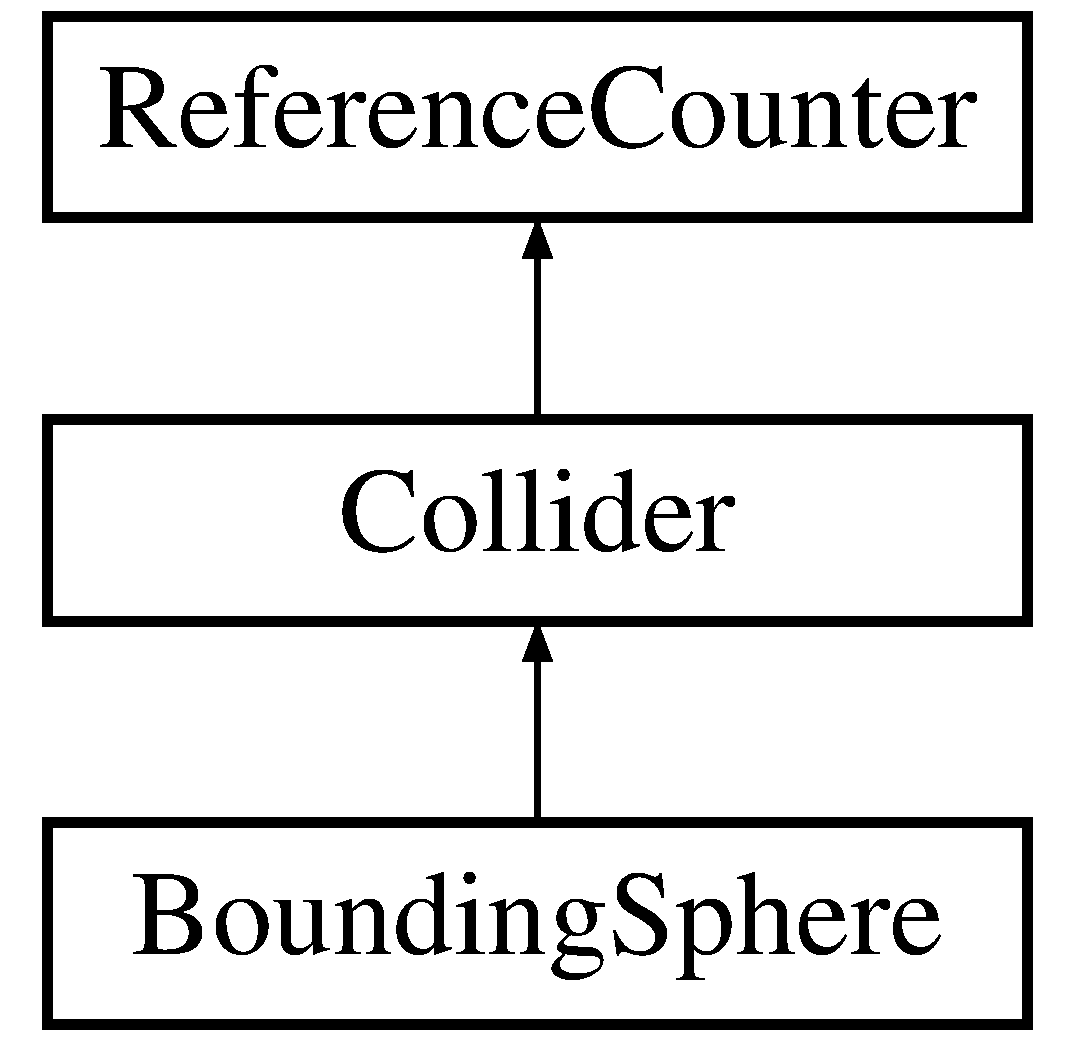
\includegraphics[height=3.000000cm]{class_bounding_sphere}
\end{center}
\end{figure}
\subsection*{Public Member Functions}
\begin{DoxyCompactItemize}
\item 
\hyperlink{class_bounding_sphere_a6139e246a2611b6479073746dbb35cbd}{Bounding\+Sphere} (const \hyperlink{class_vector3f}{Vector3f} \&center, float radius)
\item 
\hyperlink{class_intersect_data}{Intersect\+Data} \hyperlink{class_bounding_sphere_a9356041ca570b82ee9e99d70a60e57d1}{Intersect\+Bounding\+Sphere} (const \hyperlink{class_bounding_sphere}{Bounding\+Sphere} \&other) const 
\item 
virtual void \hyperlink{class_bounding_sphere_a272125f529f43fb07ef026afb115ce56}{Transform} (const \hyperlink{class_vector3f}{Vector3f} \&translation)
\item 
virtual \hyperlink{class_vector3f}{Vector3f} \hyperlink{class_bounding_sphere_aa060fdf09876145ec3cebe80c769eceb}{Get\+Center} () const 
\item 
float \hyperlink{class_bounding_sphere_a40d9116ac275d1528b9477620a17d0d0}{Get\+Radius} () const 
\end{DoxyCompactItemize}
\subsection*{Static Public Member Functions}
\begin{DoxyCompactItemize}
\item 
static void \hyperlink{class_bounding_sphere_a73e8a4e978f583ace1bebcab3e32d5c2}{Test} ()
\end{DoxyCompactItemize}
\subsection*{Additional Inherited Members}


\subsection{Detailed Description}
The \hyperlink{class_bounding_sphere}{Bounding\+Sphere} class represents an sphere that can be used as a collider in a physics engine. 

\subsection{Constructor \& Destructor Documentation}
\hypertarget{class_bounding_sphere_a6139e246a2611b6479073746dbb35cbd}{}\index{Bounding\+Sphere@{Bounding\+Sphere}!Bounding\+Sphere@{Bounding\+Sphere}}
\index{Bounding\+Sphere@{Bounding\+Sphere}!Bounding\+Sphere@{Bounding\+Sphere}}
\subsubsection[{Bounding\+Sphere(const Vector3f \&center, float radius)}]{\setlength{\rightskip}{0pt plus 5cm}Bounding\+Sphere\+::\+Bounding\+Sphere (
\begin{DoxyParamCaption}
\item[{const {\bf Vector3f} \&}]{center, }
\item[{float}]{radius}
\end{DoxyParamCaption}
)\hspace{0.3cm}{\ttfamily [inline]}}\label{class_bounding_sphere_a6139e246a2611b6479073746dbb35cbd}
Creates a \hyperlink{class_bounding_sphere}{Bounding\+Sphere} in a usable state.


\begin{DoxyParams}{Parameters}
{\em center} & The center point of the sphere. \\
\hline
{\em radius} & The distance from any point on the sphere to the center. \\
\hline
\end{DoxyParams}


\subsection{Member Function Documentation}
\hypertarget{class_bounding_sphere_aa060fdf09876145ec3cebe80c769eceb}{}\index{Bounding\+Sphere@{Bounding\+Sphere}!Get\+Center@{Get\+Center}}
\index{Get\+Center@{Get\+Center}!Bounding\+Sphere@{Bounding\+Sphere}}
\subsubsection[{Get\+Center() const }]{\setlength{\rightskip}{0pt plus 5cm}virtual {\bf Vector3f} Bounding\+Sphere\+::\+Get\+Center (
\begin{DoxyParamCaption}
{}
\end{DoxyParamCaption}
) const\hspace{0.3cm}{\ttfamily [inline]}, {\ttfamily [virtual]}}\label{class_bounding_sphere_aa060fdf09876145ec3cebe80c769eceb}
Returns the center position of the collider. Should be overriden by subclasses. 

Reimplemented from \hyperlink{class_collider_ae707f012a5f8263d5262897b4a3d9ee5}{Collider}.

\hypertarget{class_bounding_sphere_a40d9116ac275d1528b9477620a17d0d0}{}\index{Bounding\+Sphere@{Bounding\+Sphere}!Get\+Radius@{Get\+Radius}}
\index{Get\+Radius@{Get\+Radius}!Bounding\+Sphere@{Bounding\+Sphere}}
\subsubsection[{Get\+Radius() const }]{\setlength{\rightskip}{0pt plus 5cm}float Bounding\+Sphere\+::\+Get\+Radius (
\begin{DoxyParamCaption}
{}
\end{DoxyParamCaption}
) const\hspace{0.3cm}{\ttfamily [inline]}}\label{class_bounding_sphere_a40d9116ac275d1528b9477620a17d0d0}
Basic getter for the radius \hypertarget{class_bounding_sphere_a9356041ca570b82ee9e99d70a60e57d1}{}\index{Bounding\+Sphere@{Bounding\+Sphere}!Intersect\+Bounding\+Sphere@{Intersect\+Bounding\+Sphere}}
\index{Intersect\+Bounding\+Sphere@{Intersect\+Bounding\+Sphere}!Bounding\+Sphere@{Bounding\+Sphere}}
\subsubsection[{Intersect\+Bounding\+Sphere(const Bounding\+Sphere \&other) const }]{\setlength{\rightskip}{0pt plus 5cm}{\bf Intersect\+Data} Bounding\+Sphere\+::\+Intersect\+Bounding\+Sphere (
\begin{DoxyParamCaption}
\item[{const {\bf Bounding\+Sphere} \&}]{other}
\end{DoxyParamCaption}
) const}\label{class_bounding_sphere_a9356041ca570b82ee9e99d70a60e57d1}
Computes information about if this sphere intersects another aphere.


\begin{DoxyParams}{Parameters}
{\em other} & The sphere that\textquotesingle{}s being tested for intersection with this sphere. \\
\hline
\end{DoxyParams}
\hypertarget{class_bounding_sphere_a73e8a4e978f583ace1bebcab3e32d5c2}{}\index{Bounding\+Sphere@{Bounding\+Sphere}!Test@{Test}}
\index{Test@{Test}!Bounding\+Sphere@{Bounding\+Sphere}}
\subsubsection[{Test()}]{\setlength{\rightskip}{0pt plus 5cm}void Bounding\+Sphere\+::\+Test (
\begin{DoxyParamCaption}
{}
\end{DoxyParamCaption}
)\hspace{0.3cm}{\ttfamily [static]}}\label{class_bounding_sphere_a73e8a4e978f583ace1bebcab3e32d5c2}
Performs a Unit Test of this class \hypertarget{class_bounding_sphere_a272125f529f43fb07ef026afb115ce56}{}\index{Bounding\+Sphere@{Bounding\+Sphere}!Transform@{Transform}}
\index{Transform@{Transform}!Bounding\+Sphere@{Bounding\+Sphere}}
\subsubsection[{Transform(const Vector3f \&translation)}]{\setlength{\rightskip}{0pt plus 5cm}void Bounding\+Sphere\+::\+Transform (
\begin{DoxyParamCaption}
\item[{const {\bf Vector3f} \&}]{translation}
\end{DoxyParamCaption}
)\hspace{0.3cm}{\ttfamily [virtual]}}\label{class_bounding_sphere_a272125f529f43fb07ef026afb115ce56}
Moves the entire collider by translation distance. Should be overriden by subclasses.


\begin{DoxyParams}{Parameters}
{\em translation} & Distance to move the collider \\
\hline
\end{DoxyParams}


Reimplemented from \hyperlink{class_collider_af15ebbef03988c4c0dffdf1fa65eb72f}{Collider}.



The documentation for this class was generated from the following files\+:\begin{DoxyCompactItemize}
\item 
F\+:/\+Fusion3\+D\+\_\+work/src/physics/\hyperlink{bounding_sphere_8h}{bounding\+Sphere.\+h}\item 
F\+:/\+Fusion3\+D\+\_\+work/src/physics/\hyperlink{bounding_sphere_8cpp}{bounding\+Sphere.\+cpp}\end{DoxyCompactItemize}

\hypertarget{class_camera}{}\section{Camera Class Reference}
\label{class_camera}\index{Camera@{Camera}}


{\ttfamily \#include $<$camera.\+h$>$}

\subsection*{Public Member Functions}
\begin{DoxyCompactItemize}
\item 
\hyperlink{class_camera_a51b0d4b1a6552dd0d3d6c6a60e505d0e}{Camera} (const \hyperlink{math3d_8h_a5b7721ab7216c91a40538beaa9e6ee1f}{Matrix4f} \&projection, \hyperlink{class_transform}{Transform} $\ast$transform)
\item 
\hyperlink{class_transform}{Transform} $\ast$ \hyperlink{class_camera_ae1937794b5efed6cb11a73c5fc3c98ab}{Get\+Transform} ()
\item 
const \hyperlink{class_transform}{Transform} \& \hyperlink{class_camera_adafb81d278c3566dad4d6fa4da7efd5f}{Get\+Transform} () const 
\item 
\hyperlink{math3d_8h_a5b7721ab7216c91a40538beaa9e6ee1f}{Matrix4f} \hyperlink{class_camera_a88e084445b0096c581707cb656333b2a}{Get\+View\+Projection} () const 
\item 
void \hyperlink{class_camera_a82ee584dbca05d545d39cb49520e0ac5}{Set\+Projection} (const \hyperlink{math3d_8h_a5b7721ab7216c91a40538beaa9e6ee1f}{Matrix4f} \&projection)
\item 
void \hyperlink{class_camera_ac643febc45392fe1df869faf7162d365}{Set\+Transform} (\hyperlink{class_transform}{Transform} $\ast$transform)
\end{DoxyCompactItemize}


\subsection{Constructor \& Destructor Documentation}
\hypertarget{class_camera_a51b0d4b1a6552dd0d3d6c6a60e505d0e}{}\index{Camera@{Camera}!Camera@{Camera}}
\index{Camera@{Camera}!Camera@{Camera}}
\subsubsection[{Camera(const Matrix4f \&projection, Transform $\ast$transform)}]{\setlength{\rightskip}{0pt plus 5cm}Camera\+::\+Camera (
\begin{DoxyParamCaption}
\item[{const {\bf Matrix4f} \&}]{projection, }
\item[{{\bf Transform} $\ast$}]{transform}
\end{DoxyParamCaption}
)\hspace{0.3cm}{\ttfamily [inline]}}\label{class_camera_a51b0d4b1a6552dd0d3d6c6a60e505d0e}


\subsection{Member Function Documentation}
\hypertarget{class_camera_ae1937794b5efed6cb11a73c5fc3c98ab}{}\index{Camera@{Camera}!Get\+Transform@{Get\+Transform}}
\index{Get\+Transform@{Get\+Transform}!Camera@{Camera}}
\subsubsection[{Get\+Transform()}]{\setlength{\rightskip}{0pt plus 5cm}{\bf Transform}$\ast$ Camera\+::\+Get\+Transform (
\begin{DoxyParamCaption}
{}
\end{DoxyParamCaption}
)\hspace{0.3cm}{\ttfamily [inline]}}\label{class_camera_ae1937794b5efed6cb11a73c5fc3c98ab}
\hypertarget{class_camera_adafb81d278c3566dad4d6fa4da7efd5f}{}\index{Camera@{Camera}!Get\+Transform@{Get\+Transform}}
\index{Get\+Transform@{Get\+Transform}!Camera@{Camera}}
\subsubsection[{Get\+Transform() const }]{\setlength{\rightskip}{0pt plus 5cm}const {\bf Transform}\& Camera\+::\+Get\+Transform (
\begin{DoxyParamCaption}
{}
\end{DoxyParamCaption}
) const\hspace{0.3cm}{\ttfamily [inline]}}\label{class_camera_adafb81d278c3566dad4d6fa4da7efd5f}
\hypertarget{class_camera_a88e084445b0096c581707cb656333b2a}{}\index{Camera@{Camera}!Get\+View\+Projection@{Get\+View\+Projection}}
\index{Get\+View\+Projection@{Get\+View\+Projection}!Camera@{Camera}}
\subsubsection[{Get\+View\+Projection() const }]{\setlength{\rightskip}{0pt plus 5cm}{\bf Matrix4f} Camera\+::\+Get\+View\+Projection (
\begin{DoxyParamCaption}
{}
\end{DoxyParamCaption}
) const}\label{class_camera_a88e084445b0096c581707cb656333b2a}
\hypertarget{class_camera_a82ee584dbca05d545d39cb49520e0ac5}{}\index{Camera@{Camera}!Set\+Projection@{Set\+Projection}}
\index{Set\+Projection@{Set\+Projection}!Camera@{Camera}}
\subsubsection[{Set\+Projection(const Matrix4f \&projection)}]{\setlength{\rightskip}{0pt plus 5cm}void Camera\+::\+Set\+Projection (
\begin{DoxyParamCaption}
\item[{const {\bf Matrix4f} \&}]{projection}
\end{DoxyParamCaption}
)\hspace{0.3cm}{\ttfamily [inline]}}\label{class_camera_a82ee584dbca05d545d39cb49520e0ac5}
\hypertarget{class_camera_ac643febc45392fe1df869faf7162d365}{}\index{Camera@{Camera}!Set\+Transform@{Set\+Transform}}
\index{Set\+Transform@{Set\+Transform}!Camera@{Camera}}
\subsubsection[{Set\+Transform(\+Transform $\ast$transform)}]{\setlength{\rightskip}{0pt plus 5cm}void Camera\+::\+Set\+Transform (
\begin{DoxyParamCaption}
\item[{{\bf Transform} $\ast$}]{transform}
\end{DoxyParamCaption}
)\hspace{0.3cm}{\ttfamily [inline]}}\label{class_camera_ac643febc45392fe1df869faf7162d365}


The documentation for this class was generated from the following files\+:\begin{DoxyCompactItemize}
\item 
F\+:/\+Fusion3\+D\+\_\+work/src/rendering/\hyperlink{camera_8h}{camera.\+h}\item 
F\+:/\+Fusion3\+D\+\_\+work/src/rendering/\hyperlink{camera_8cpp}{camera.\+cpp}\end{DoxyCompactItemize}

\hypertarget{structchunk}{}\section{chunk Struct Reference}
\label{structchunk}\index{chunk@{chunk}}
\subsection*{Public Attributes}
\begin{DoxyCompactItemize}
\item 
\hyperlink{stb__image_8c_a1134b580f8da4de94ca6b1de4d37975e}{uint32} \hyperlink{structchunk_a0b5cc0c5a9b91945c42373db2a499fb1}{length}
\item 
\hyperlink{stb__image_8c_a1134b580f8da4de94ca6b1de4d37975e}{uint32} \hyperlink{structchunk_a05d5489f3807bc7ba149c1904241d087}{type}
\end{DoxyCompactItemize}


\subsection{Member Data Documentation}
\hypertarget{structchunk_a0b5cc0c5a9b91945c42373db2a499fb1}{}\index{chunk@{chunk}!length@{length}}
\index{length@{length}!chunk@{chunk}}
\subsubsection[{length}]{\setlength{\rightskip}{0pt plus 5cm}{\bf uint32} chunk\+::length}\label{structchunk_a0b5cc0c5a9b91945c42373db2a499fb1}
\hypertarget{structchunk_a05d5489f3807bc7ba149c1904241d087}{}\index{chunk@{chunk}!type@{type}}
\index{type@{type}!chunk@{chunk}}
\subsubsection[{type}]{\setlength{\rightskip}{0pt plus 5cm}{\bf uint32} chunk\+::type}\label{structchunk_a05d5489f3807bc7ba149c1904241d087}


The documentation for this struct was generated from the following file\+:\begin{DoxyCompactItemize}
\item 
F\+:/\+Fusion3\+D\+\_\+work/src/static\+Libs/\hyperlink{stb__image_8c}{stb\+\_\+image.\+c}\end{DoxyCompactItemize}

\hypertarget{class_collider}{}\section{Collider Class Reference}
\label{class_collider}\index{Collider@{Collider}}


{\ttfamily \#include $<$collider.\+h$>$}

Inheritance diagram for Collider\+:\begin{figure}[H]
\begin{center}
\leavevmode
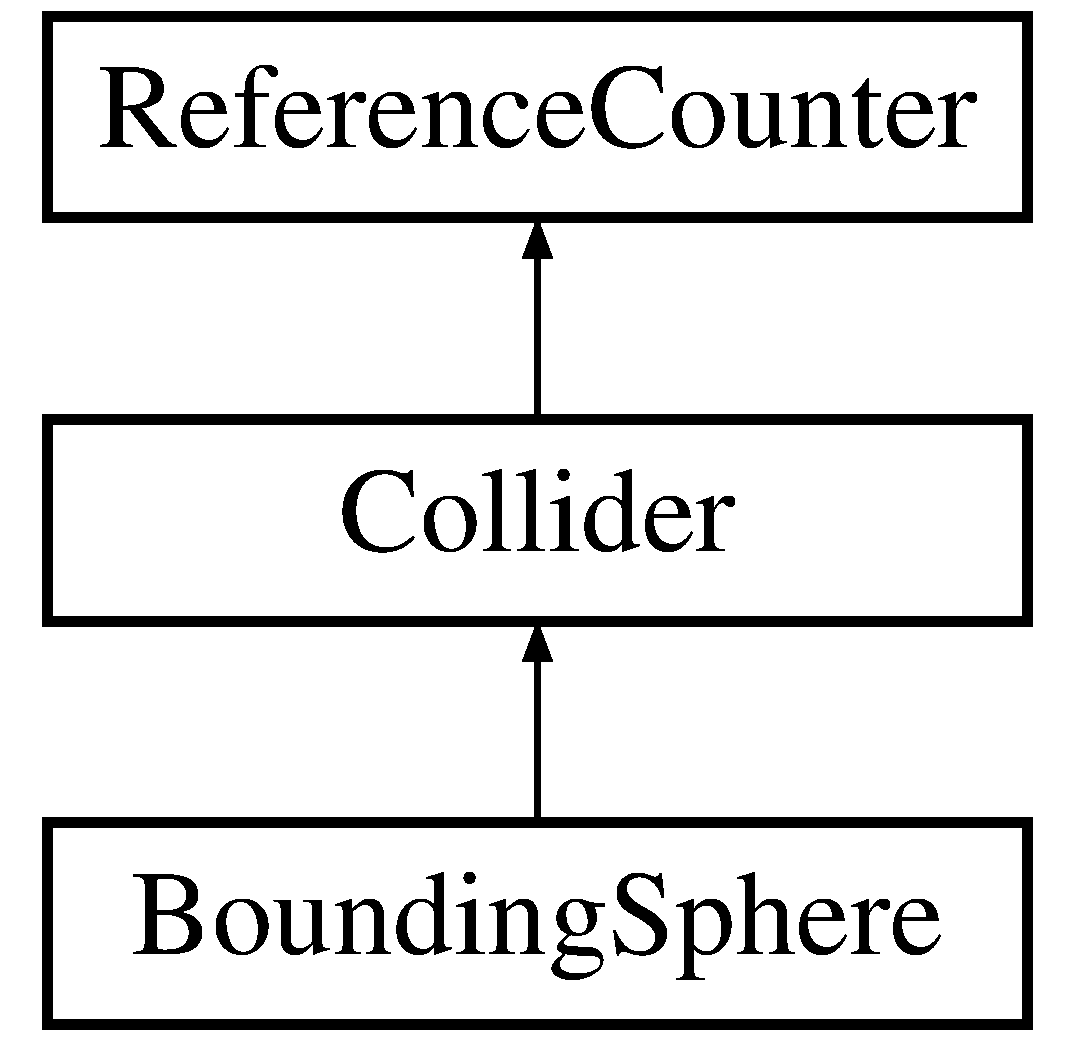
\includegraphics[height=3.000000cm]{class_collider}
\end{center}
\end{figure}
\subsection*{Public Types}
\begin{DoxyCompactItemize}
\item 
enum \{ \hyperlink{class_collider_a63b6ff66c4e92905d981551006239987aedae9a0a3179b58ac15c0616035042e2}{T\+Y\+P\+E\+\_\+\+S\+P\+H\+E\+R\+E}, 
\hyperlink{class_collider_a63b6ff66c4e92905d981551006239987a77aeb0be239c46a6adbf47df8eb3123c}{T\+Y\+P\+E\+\_\+\+A\+A\+B\+B}, 
\hyperlink{class_collider_a63b6ff66c4e92905d981551006239987ae839bd8ef09a93bd5b4bcb8c6cec9251}{T\+Y\+P\+E\+\_\+\+S\+I\+Z\+E}
 \}
\end{DoxyCompactItemize}
\subsection*{Public Member Functions}
\begin{DoxyCompactItemize}
\item 
\hyperlink{class_collider_a3fed523e82fb51e73bf97c7690163afe}{Collider} (int type)
\item 
\hyperlink{class_intersect_data}{Intersect\+Data} \hyperlink{class_collider_a3d2665cd1c5e8142c9c960cc68316e92}{Intersect} (const \hyperlink{class_collider}{Collider} \&other) const 
\item 
virtual void \hyperlink{class_collider_af15ebbef03988c4c0dffdf1fa65eb72f}{Transform} (const \hyperlink{class_vector3f}{Vector3f} \&translation)
\item 
virtual \hyperlink{class_vector3f}{Vector3f} \hyperlink{class_collider_ae707f012a5f8263d5262897b4a3d9ee5}{Get\+Center} () const 
\item 
int \hyperlink{class_collider_a3c68244a12cd4f973e5d4eeaad599a32}{Get\+Type} () const 
\end{DoxyCompactItemize}


\subsection{Detailed Description}
The \hyperlink{class_collider}{Collider} class is the base class for colliders that can be used in the physics engine. More specific colliders should inherit from this class 

\subsection{Member Enumeration Documentation}
\hypertarget{class_collider_a63b6ff66c4e92905d981551006239987}{}\subsubsection[{anonymous enum}]{\setlength{\rightskip}{0pt plus 5cm}anonymous enum}\label{class_collider_a63b6ff66c4e92905d981551006239987}
This enumeration stores all the types of colliders that can be used. \begin{Desc}
\item[Enumerator]\par
\begin{description}
\index{T\+Y\+P\+E\+\_\+\+S\+P\+H\+E\+R\+E@{T\+Y\+P\+E\+\_\+\+S\+P\+H\+E\+R\+E}!Collider@{Collider}}\index{Collider@{Collider}!T\+Y\+P\+E\+\_\+\+S\+P\+H\+E\+R\+E@{T\+Y\+P\+E\+\_\+\+S\+P\+H\+E\+R\+E}}\item[{\em 
\hypertarget{class_collider_a63b6ff66c4e92905d981551006239987aedae9a0a3179b58ac15c0616035042e2}{}T\+Y\+P\+E\+\_\+\+S\+P\+H\+E\+R\+E\label{class_collider_a63b6ff66c4e92905d981551006239987aedae9a0a3179b58ac15c0616035042e2}
}]\index{T\+Y\+P\+E\+\_\+\+A\+A\+B\+B@{T\+Y\+P\+E\+\_\+\+A\+A\+B\+B}!Collider@{Collider}}\index{Collider@{Collider}!T\+Y\+P\+E\+\_\+\+A\+A\+B\+B@{T\+Y\+P\+E\+\_\+\+A\+A\+B\+B}}\item[{\em 
\hypertarget{class_collider_a63b6ff66c4e92905d981551006239987a77aeb0be239c46a6adbf47df8eb3123c}{}T\+Y\+P\+E\+\_\+\+A\+A\+B\+B\label{class_collider_a63b6ff66c4e92905d981551006239987a77aeb0be239c46a6adbf47df8eb3123c}
}]\index{T\+Y\+P\+E\+\_\+\+S\+I\+Z\+E@{T\+Y\+P\+E\+\_\+\+S\+I\+Z\+E}!Collider@{Collider}}\index{Collider@{Collider}!T\+Y\+P\+E\+\_\+\+S\+I\+Z\+E@{T\+Y\+P\+E\+\_\+\+S\+I\+Z\+E}}\item[{\em 
\hypertarget{class_collider_a63b6ff66c4e92905d981551006239987ae839bd8ef09a93bd5b4bcb8c6cec9251}{}T\+Y\+P\+E\+\_\+\+S\+I\+Z\+E\label{class_collider_a63b6ff66c4e92905d981551006239987ae839bd8ef09a93bd5b4bcb8c6cec9251}
}]\end{description}
\end{Desc}


\subsection{Constructor \& Destructor Documentation}
\hypertarget{class_collider_a3fed523e82fb51e73bf97c7690163afe}{}\index{Collider@{Collider}!Collider@{Collider}}
\index{Collider@{Collider}!Collider@{Collider}}
\subsubsection[{Collider(int type)}]{\setlength{\rightskip}{0pt plus 5cm}Collider\+::\+Collider (
\begin{DoxyParamCaption}
\item[{int}]{type}
\end{DoxyParamCaption}
)\hspace{0.3cm}{\ttfamily [inline]}}\label{class_collider_a3fed523e82fb51e73bf97c7690163afe}
Creates a \hyperlink{class_collider}{Collider} in a usable state.


\begin{DoxyParams}{Parameters}
{\em type} & The type of collider this represents. \\
\hline
\end{DoxyParams}


\subsection{Member Function Documentation}
\hypertarget{class_collider_ae707f012a5f8263d5262897b4a3d9ee5}{}\index{Collider@{Collider}!Get\+Center@{Get\+Center}}
\index{Get\+Center@{Get\+Center}!Collider@{Collider}}
\subsubsection[{Get\+Center() const }]{\setlength{\rightskip}{0pt plus 5cm}virtual {\bf Vector3f} Collider\+::\+Get\+Center (
\begin{DoxyParamCaption}
{}
\end{DoxyParamCaption}
) const\hspace{0.3cm}{\ttfamily [inline]}, {\ttfamily [virtual]}}\label{class_collider_ae707f012a5f8263d5262897b4a3d9ee5}
Returns the center position of the collider. Should be overriden by subclasses. 

Reimplemented in \hyperlink{class_bounding_sphere_aa060fdf09876145ec3cebe80c769eceb}{Bounding\+Sphere}.

\hypertarget{class_collider_a3c68244a12cd4f973e5d4eeaad599a32}{}\index{Collider@{Collider}!Get\+Type@{Get\+Type}}
\index{Get\+Type@{Get\+Type}!Collider@{Collider}}
\subsubsection[{Get\+Type() const }]{\setlength{\rightskip}{0pt plus 5cm}int Collider\+::\+Get\+Type (
\begin{DoxyParamCaption}
{}
\end{DoxyParamCaption}
) const\hspace{0.3cm}{\ttfamily [inline]}}\label{class_collider_a3c68244a12cd4f973e5d4eeaad599a32}
Basic getter \hypertarget{class_collider_a3d2665cd1c5e8142c9c960cc68316e92}{}\index{Collider@{Collider}!Intersect@{Intersect}}
\index{Intersect@{Intersect}!Collider@{Collider}}
\subsubsection[{Intersect(const Collider \&other) const }]{\setlength{\rightskip}{0pt plus 5cm}{\bf Intersect\+Data} Collider\+::\+Intersect (
\begin{DoxyParamCaption}
\item[{const {\bf Collider} \&}]{other}
\end{DoxyParamCaption}
) const}\label{class_collider_a3d2665cd1c5e8142c9c960cc68316e92}
Calculates information about if this collider is intersecting with another collider.


\begin{DoxyParams}{Parameters}
{\em other} & The collider that is being checked for intersection. \\
\hline
\end{DoxyParams}
\hypertarget{class_collider_af15ebbef03988c4c0dffdf1fa65eb72f}{}\index{Collider@{Collider}!Transform@{Transform}}
\index{Transform@{Transform}!Collider@{Collider}}
\subsubsection[{Transform(const Vector3f \&translation)}]{\setlength{\rightskip}{0pt plus 5cm}virtual void Collider\+::\+Transform (
\begin{DoxyParamCaption}
\item[{const {\bf Vector3f} \&}]{translation}
\end{DoxyParamCaption}
)\hspace{0.3cm}{\ttfamily [inline]}, {\ttfamily [virtual]}}\label{class_collider_af15ebbef03988c4c0dffdf1fa65eb72f}
Moves the entire collider by translation distance. Should be overriden by subclasses.


\begin{DoxyParams}{Parameters}
{\em translation} & Distance to move the collider \\
\hline
\end{DoxyParams}


Reimplemented in \hyperlink{class_bounding_sphere_a272125f529f43fb07ef026afb115ce56}{Bounding\+Sphere}.



The documentation for this class was generated from the following files\+:\begin{DoxyCompactItemize}
\item 
F\+:/\+Fusion3\+D\+\_\+work/src/physics/\hyperlink{collider_8h}{collider.\+h}\item 
F\+:/\+Fusion3\+D\+\_\+work/src/physics/\hyperlink{collider_8cpp}{collider.\+cpp}\end{DoxyCompactItemize}

\hypertarget{class_core_engine}{}\section{Core\+Engine Class Reference}
\label{class_core_engine}\index{Core\+Engine@{Core\+Engine}}


{\ttfamily \#include $<$core\+Engine.\+h$>$}

\subsection*{Public Member Functions}
\begin{DoxyCompactItemize}
\item 
\hyperlink{class_core_engine_ad828ebdde32d2b749c2e6d5c6ea9460a}{Core\+Engine} (double frame\+Rate, \hyperlink{class_window}{Window} $\ast$window, \hyperlink{class_rendering_engine}{Rendering\+Engine} $\ast$rendering\+Engine, \hyperlink{class_physics_engine}{Physics\+Engine} $\ast$physics\+Engine, \hyperlink{class_game}{Game} $\ast$game)
\item 
void \hyperlink{class_core_engine_a846ab7b6441f17ceef54ceb7045e891b}{Start} ()
\item 
void \hyperlink{class_core_engine_a18b890c2dafcb841c8b45d0e324ab068}{Stop} ()
\item 
\hyperlink{class_rendering_engine}{Rendering\+Engine} $\ast$ \hyperlink{class_core_engine_a347a39ec08bde097dd93d50fc850e7a1}{Get\+Rendering\+Engine} ()
\item 
\hyperlink{class_physics_engine}{Physics\+Engine} $\ast$ \hyperlink{class_core_engine_acb446732d06178f55eda89ef32bab7b5}{Get\+Physics\+Engine} ()
\item 
void \hyperlink{class_core_engine_a49789f1b66c018e944e9e3929a896738}{Set\+Simulation} (bool state)
\item 
bool \hyperlink{class_core_engine_a9facc85782ab5112ba80aada6d2a1214}{Get\+Simulation} () const 
\end{DoxyCompactItemize}
\subsection*{Static Public Member Functions}
\begin{DoxyCompactItemize}
\item 
static \hyperlink{class_core_engine}{Core\+Engine} $\ast$ \hyperlink{class_core_engine_a66fa2bc850f4922acd44769ade1d42dd}{Get\+Core\+Engine} ()
\item 
static void \hyperlink{class_core_engine_a990a9435f091ec88762677f7830225ba}{Set\+Core\+Engine} (\hyperlink{class_core_engine}{Core\+Engine} $\ast$core\+Engine)
\end{DoxyCompactItemize}


\subsection{Constructor \& Destructor Documentation}
\hypertarget{class_core_engine_ad828ebdde32d2b749c2e6d5c6ea9460a}{}\index{Core\+Engine@{Core\+Engine}!Core\+Engine@{Core\+Engine}}
\index{Core\+Engine@{Core\+Engine}!Core\+Engine@{Core\+Engine}}
\subsubsection[{Core\+Engine(double frame\+Rate, Window $\ast$window, Rendering\+Engine $\ast$rendering\+Engine, Physics\+Engine $\ast$physics\+Engine, Game $\ast$game)}]{\setlength{\rightskip}{0pt plus 5cm}Core\+Engine\+::\+Core\+Engine (
\begin{DoxyParamCaption}
\item[{double}]{frame\+Rate, }
\item[{{\bf Window} $\ast$}]{window, }
\item[{{\bf Rendering\+Engine} $\ast$}]{rendering\+Engine, }
\item[{{\bf Physics\+Engine} $\ast$}]{physics\+Engine, }
\item[{{\bf Game} $\ast$}]{game}
\end{DoxyParamCaption}
)}\label{class_core_engine_ad828ebdde32d2b749c2e6d5c6ea9460a}


\subsection{Member Function Documentation}
\hypertarget{class_core_engine_a66fa2bc850f4922acd44769ade1d42dd}{}\index{Core\+Engine@{Core\+Engine}!Get\+Core\+Engine@{Get\+Core\+Engine}}
\index{Get\+Core\+Engine@{Get\+Core\+Engine}!Core\+Engine@{Core\+Engine}}
\subsubsection[{Get\+Core\+Engine()}]{\setlength{\rightskip}{0pt plus 5cm}static {\bf Core\+Engine}$\ast$ Core\+Engine\+::\+Get\+Core\+Engine (
\begin{DoxyParamCaption}
{}
\end{DoxyParamCaption}
)\hspace{0.3cm}{\ttfamily [inline]}, {\ttfamily [static]}}\label{class_core_engine_a66fa2bc850f4922acd44769ade1d42dd}
\hypertarget{class_core_engine_acb446732d06178f55eda89ef32bab7b5}{}\index{Core\+Engine@{Core\+Engine}!Get\+Physics\+Engine@{Get\+Physics\+Engine}}
\index{Get\+Physics\+Engine@{Get\+Physics\+Engine}!Core\+Engine@{Core\+Engine}}
\subsubsection[{Get\+Physics\+Engine()}]{\setlength{\rightskip}{0pt plus 5cm}{\bf Physics\+Engine}$\ast$ Core\+Engine\+::\+Get\+Physics\+Engine (
\begin{DoxyParamCaption}
{}
\end{DoxyParamCaption}
)\hspace{0.3cm}{\ttfamily [inline]}}\label{class_core_engine_acb446732d06178f55eda89ef32bab7b5}
\hypertarget{class_core_engine_a347a39ec08bde097dd93d50fc850e7a1}{}\index{Core\+Engine@{Core\+Engine}!Get\+Rendering\+Engine@{Get\+Rendering\+Engine}}
\index{Get\+Rendering\+Engine@{Get\+Rendering\+Engine}!Core\+Engine@{Core\+Engine}}
\subsubsection[{Get\+Rendering\+Engine()}]{\setlength{\rightskip}{0pt plus 5cm}{\bf Rendering\+Engine}$\ast$ Core\+Engine\+::\+Get\+Rendering\+Engine (
\begin{DoxyParamCaption}
{}
\end{DoxyParamCaption}
)\hspace{0.3cm}{\ttfamily [inline]}}\label{class_core_engine_a347a39ec08bde097dd93d50fc850e7a1}
\hypertarget{class_core_engine_a9facc85782ab5112ba80aada6d2a1214}{}\index{Core\+Engine@{Core\+Engine}!Get\+Simulation@{Get\+Simulation}}
\index{Get\+Simulation@{Get\+Simulation}!Core\+Engine@{Core\+Engine}}
\subsubsection[{Get\+Simulation() const }]{\setlength{\rightskip}{0pt plus 5cm}bool Core\+Engine\+::\+Get\+Simulation (
\begin{DoxyParamCaption}
{}
\end{DoxyParamCaption}
) const\hspace{0.3cm}{\ttfamily [inline]}}\label{class_core_engine_a9facc85782ab5112ba80aada6d2a1214}
\hypertarget{class_core_engine_a990a9435f091ec88762677f7830225ba}{}\index{Core\+Engine@{Core\+Engine}!Set\+Core\+Engine@{Set\+Core\+Engine}}
\index{Set\+Core\+Engine@{Set\+Core\+Engine}!Core\+Engine@{Core\+Engine}}
\subsubsection[{Set\+Core\+Engine(\+Core\+Engine $\ast$core\+Engine)}]{\setlength{\rightskip}{0pt plus 5cm}static void Core\+Engine\+::\+Set\+Core\+Engine (
\begin{DoxyParamCaption}
\item[{{\bf Core\+Engine} $\ast$}]{core\+Engine}
\end{DoxyParamCaption}
)\hspace{0.3cm}{\ttfamily [inline]}, {\ttfamily [static]}}\label{class_core_engine_a990a9435f091ec88762677f7830225ba}
\hypertarget{class_core_engine_a49789f1b66c018e944e9e3929a896738}{}\index{Core\+Engine@{Core\+Engine}!Set\+Simulation@{Set\+Simulation}}
\index{Set\+Simulation@{Set\+Simulation}!Core\+Engine@{Core\+Engine}}
\subsubsection[{Set\+Simulation(bool state)}]{\setlength{\rightskip}{0pt plus 5cm}void Core\+Engine\+::\+Set\+Simulation (
\begin{DoxyParamCaption}
\item[{bool}]{state}
\end{DoxyParamCaption}
)\hspace{0.3cm}{\ttfamily [inline]}}\label{class_core_engine_a49789f1b66c018e944e9e3929a896738}
\hypertarget{class_core_engine_a846ab7b6441f17ceef54ceb7045e891b}{}\index{Core\+Engine@{Core\+Engine}!Start@{Start}}
\index{Start@{Start}!Core\+Engine@{Core\+Engine}}
\subsubsection[{Start()}]{\setlength{\rightskip}{0pt plus 5cm}void Core\+Engine\+::\+Start (
\begin{DoxyParamCaption}
{}
\end{DoxyParamCaption}
)}\label{class_core_engine_a846ab7b6441f17ceef54ceb7045e891b}
\hypertarget{class_core_engine_a18b890c2dafcb841c8b45d0e324ab068}{}\index{Core\+Engine@{Core\+Engine}!Stop@{Stop}}
\index{Stop@{Stop}!Core\+Engine@{Core\+Engine}}
\subsubsection[{Stop()}]{\setlength{\rightskip}{0pt plus 5cm}void Core\+Engine\+::\+Stop (
\begin{DoxyParamCaption}
{}
\end{DoxyParamCaption}
)}\label{class_core_engine_a18b890c2dafcb841c8b45d0e324ab068}


The documentation for this class was generated from the following files\+:\begin{DoxyCompactItemize}
\item 
F\+:/\+Fusion3\+D\+\_\+work/src/core/\hyperlink{core_engine_8h}{core\+Engine.\+h}\item 
F\+:/\+Fusion3\+D\+\_\+work/src/core/\hyperlink{core_engine_8cpp}{core\+Engine.\+cpp}\end{DoxyCompactItemize}

\hypertarget{class_delay_timer}{}\section{Delay\+Timer Class Reference}
\label{class_delay_timer}\index{Delay\+Timer@{Delay\+Timer}}


{\ttfamily \#include $<$timing.\+h$>$}

\subsection*{Public Member Functions}
\begin{DoxyCompactItemize}
\item 
\hyperlink{class_delay_timer_ae59950e288b417f361d4c987e52fad6b}{Delay\+Timer} ()
\item 
\hyperlink{class_delay_timer_a1fdf91396e5375017999cd419125d5fe}{Delay\+Timer} (double delay)
\item 
double \hyperlink{class_delay_timer_ae659aa58558d8b87d98a69bdcc53ae56}{Get\+Delay} () const 
\item 
void \hyperlink{class_delay_timer_a03a384a4cf0ab7b496c6c94f3eeaf564}{Set\+Delay} (double delay)
\item 
int \hyperlink{class_delay_timer_a1432bc52887bab17358c7ae25a3f27c9}{Has\+Elapsed} ()
\end{DoxyCompactItemize}


\subsection{Constructor \& Destructor Documentation}
\hypertarget{class_delay_timer_ae59950e288b417f361d4c987e52fad6b}{}\index{Delay\+Timer@{Delay\+Timer}!Delay\+Timer@{Delay\+Timer}}
\index{Delay\+Timer@{Delay\+Timer}!Delay\+Timer@{Delay\+Timer}}
\subsubsection[{Delay\+Timer()}]{\setlength{\rightskip}{0pt plus 5cm}Delay\+Timer\+::\+Delay\+Timer (
\begin{DoxyParamCaption}
{}
\end{DoxyParamCaption}
)\hspace{0.3cm}{\ttfamily [inline]}}\label{class_delay_timer_ae59950e288b417f361d4c987e52fad6b}
\hypertarget{class_delay_timer_a1fdf91396e5375017999cd419125d5fe}{}\index{Delay\+Timer@{Delay\+Timer}!Delay\+Timer@{Delay\+Timer}}
\index{Delay\+Timer@{Delay\+Timer}!Delay\+Timer@{Delay\+Timer}}
\subsubsection[{Delay\+Timer(double delay)}]{\setlength{\rightskip}{0pt plus 5cm}Delay\+Timer\+::\+Delay\+Timer (
\begin{DoxyParamCaption}
\item[{double}]{delay}
\end{DoxyParamCaption}
)\hspace{0.3cm}{\ttfamily [inline]}}\label{class_delay_timer_a1fdf91396e5375017999cd419125d5fe}


\subsection{Member Function Documentation}
\hypertarget{class_delay_timer_ae659aa58558d8b87d98a69bdcc53ae56}{}\index{Delay\+Timer@{Delay\+Timer}!Get\+Delay@{Get\+Delay}}
\index{Get\+Delay@{Get\+Delay}!Delay\+Timer@{Delay\+Timer}}
\subsubsection[{Get\+Delay() const }]{\setlength{\rightskip}{0pt plus 5cm}double Delay\+Timer\+::\+Get\+Delay (
\begin{DoxyParamCaption}
{}
\end{DoxyParamCaption}
) const\hspace{0.3cm}{\ttfamily [inline]}}\label{class_delay_timer_ae659aa58558d8b87d98a69bdcc53ae56}
\hypertarget{class_delay_timer_a1432bc52887bab17358c7ae25a3f27c9}{}\index{Delay\+Timer@{Delay\+Timer}!Has\+Elapsed@{Has\+Elapsed}}
\index{Has\+Elapsed@{Has\+Elapsed}!Delay\+Timer@{Delay\+Timer}}
\subsubsection[{Has\+Elapsed()}]{\setlength{\rightskip}{0pt plus 5cm}int Delay\+Timer\+::\+Has\+Elapsed (
\begin{DoxyParamCaption}
{}
\end{DoxyParamCaption}
)\hspace{0.3cm}{\ttfamily [inline]}}\label{class_delay_timer_a1432bc52887bab17358c7ae25a3f27c9}
\hypertarget{class_delay_timer_a03a384a4cf0ab7b496c6c94f3eeaf564}{}\index{Delay\+Timer@{Delay\+Timer}!Set\+Delay@{Set\+Delay}}
\index{Set\+Delay@{Set\+Delay}!Delay\+Timer@{Delay\+Timer}}
\subsubsection[{Set\+Delay(double delay)}]{\setlength{\rightskip}{0pt plus 5cm}void Delay\+Timer\+::\+Set\+Delay (
\begin{DoxyParamCaption}
\item[{double}]{delay}
\end{DoxyParamCaption}
)\hspace{0.3cm}{\ttfamily [inline]}}\label{class_delay_timer_a03a384a4cf0ab7b496c6c94f3eeaf564}


The documentation for this class was generated from the following file\+:\begin{DoxyCompactItemize}
\item 
F\+:/\+Fusion3\+D\+\_\+work/src/core/\hyperlink{timing_8h}{timing.\+h}\end{DoxyCompactItemize}

\hypertarget{class_entity}{}\section{Entity Class Reference}
\label{class_entity}\index{Entity@{Entity}}


{\ttfamily \#include $<$entity.\+h$>$}

\subsection*{Public Member Functions}
\begin{DoxyCompactItemize}
\item 
\hyperlink{class_entity_a0ff4aa25e3f7d68cee620ee473d0801c}{Entity} (const \hyperlink{class_vector3f}{Vector3f} \&pos=\hyperlink{class_vector3f}{Vector3f}(0, 0, 0), const \hyperlink{class_quaternion}{Quaternion} \&rot=\hyperlink{class_quaternion}{Quaternion}(0, 0, 0, 1), float scale=1.\+0f)
\item 
virtual \hyperlink{class_entity_adf6d3f7cb1b2ba029b6b048a395cc8ae}{$\sim$\+Entity} ()
\item 
\hyperlink{class_entity}{Entity} $\ast$ \hyperlink{class_entity_a82adda07e5a8db0a7e5d0ff703a1541b}{Add\+Child} (\hyperlink{class_entity}{Entity} $\ast$child)
\item 
\hyperlink{class_entity}{Entity} $\ast$ \hyperlink{class_entity_af95f1fb0432827cf12d397bbe4c6480c}{Add\+Component} (\hyperlink{class_entity_component}{Entity\+Component} $\ast$component)
\item 
\hyperlink{class_entity}{Entity} $\ast$ \hyperlink{class_entity_a884f4b6c8de84250682f7dfaa97a34d4}{Add\+Components} (std\+::vector$<$ \hyperlink{class_entity_component}{Entity\+Component} $\ast$ $>$ components)
\item 
void \hyperlink{class_entity_a555b11eb18ebada6abb9219c316ec7c6}{Init\+All} ()
\item 
void \hyperlink{class_entity_a13845ee7d4ad92ba6bdfbe77f8da8c33}{Process\+Input\+All} (const \hyperlink{class_input}{Input} \&input, float delta)
\item 
void \hyperlink{class_entity_acfca1006fafab6577cee3c3d3af417a6}{Update\+All} (float delta)
\item 
void \hyperlink{class_entity_a6c13950fc02c20544f273b51f93f657b}{Render\+All} (const \hyperlink{class_shader}{Shader} \&shader, const \hyperlink{class_rendering_engine}{Rendering\+Engine} \&rendering\+Engine, const \hyperlink{class_camera}{Camera} \&camera) const 
\item 
void \hyperlink{class_entity_a01754307786d6d6891ccec895d7c26fa}{Post\+Render\+All} (const \hyperlink{class_shader}{Shader} \&shader, const \hyperlink{class_rendering_engine}{Rendering\+Engine} \&rendering\+Engine, const \hyperlink{class_camera}{Camera} \&camera) const 
\item 
std\+::vector$<$ \hyperlink{class_entity}{Entity} $\ast$ $>$ \hyperlink{class_entity_a77b7d12e1014fa2a128c8e3aa6d39ea3}{Get\+All\+Attached} ()
\item 
\hyperlink{class_transform}{Transform} $\ast$ \hyperlink{class_entity_a5ea21fddf63008658e00854465480034}{Get\+Transform} ()
\item 
\hyperlink{class_entity}{Entity} $\ast$ \hyperlink{class_entity_a5276811e6b06f2cdadcab05c2101ab00}{Get\+Parent} ()
\item 
void \hyperlink{class_entity_ae57c283bdba04e4d806115ff96931e94}{Set\+Engine} (\hyperlink{class_core_engine}{Core\+Engine} $\ast$engine)
\item 
void \hyperlink{class_entity_a9868d4eec27cce13c9c70d8682f82dcd}{Set\+Parent} (\hyperlink{class_entity}{Entity} $\ast$parent)
\item 
const std\+::string \& \hyperlink{class_entity_a332f7c70751b38fd8613b869769bfc9f}{Get\+Display\+Name} () const 
\item 
\hyperlink{class_entity}{Entity} $\ast$ \hyperlink{class_entity_a82d3a29a088de0e03ca7efec31616b44}{Set\+Display\+Name} (const std\+::string \&display\+Name)
\item 
void \hyperlink{class_entity_aa75151fc607686b42d27f8c3ba73143d}{Destroy} ()
\item 
\hyperlink{class_entity}{Entity} $\ast$ \hyperlink{class_entity_ab09ef7808570f70f07e18cbc1d231d39}{Get\+Scene} ()
\item 
\hyperlink{class_entity}{Entity} $\ast$ \hyperlink{class_entity_aa70bc19f38ec105785d27df0134284fb}{Get\+Child\+By\+Name} (const std\+::string \&name)
\item 
\hyperlink{class_entity_component}{Entity\+Component} $\ast$ \hyperlink{class_entity_a1e23b43bf0b76ba6ef427154eb8eea9e}{Get\+Component\+By\+Type} (const std\+::string \&name)
\end{DoxyCompactItemize}


\subsection{Constructor \& Destructor Documentation}
\hypertarget{class_entity_a0ff4aa25e3f7d68cee620ee473d0801c}{}\index{Entity@{Entity}!Entity@{Entity}}
\index{Entity@{Entity}!Entity@{Entity}}
\subsubsection[{Entity(const Vector3f \&pos=\+Vector3f(0, 0, 0), const Quaternion \&rot=\+Quaternion(0, 0, 0, 1), float scale=1.\+0f)}]{\setlength{\rightskip}{0pt plus 5cm}Entity\+::\+Entity (
\begin{DoxyParamCaption}
\item[{const {\bf Vector3f} \&}]{pos = {\ttfamily {\bf Vector3f}(0,~0,~0)}, }
\item[{const {\bf Quaternion} \&}]{rot = {\ttfamily {\bf Quaternion}(0,~0,~0,~1)}, }
\item[{float}]{scale = {\ttfamily 1.0f}}
\end{DoxyParamCaption}
)}\label{class_entity_a0ff4aa25e3f7d68cee620ee473d0801c}
\hypertarget{class_entity_adf6d3f7cb1b2ba029b6b048a395cc8ae}{}\index{Entity@{Entity}!````~Entity@{$\sim$\+Entity}}
\index{````~Entity@{$\sim$\+Entity}!Entity@{Entity}}
\subsubsection[{$\sim$\+Entity()}]{\setlength{\rightskip}{0pt plus 5cm}Entity\+::$\sim$\+Entity (
\begin{DoxyParamCaption}
{}
\end{DoxyParamCaption}
)\hspace{0.3cm}{\ttfamily [virtual]}}\label{class_entity_adf6d3f7cb1b2ba029b6b048a395cc8ae}


\subsection{Member Function Documentation}
\hypertarget{class_entity_a82adda07e5a8db0a7e5d0ff703a1541b}{}\index{Entity@{Entity}!Add\+Child@{Add\+Child}}
\index{Add\+Child@{Add\+Child}!Entity@{Entity}}
\subsubsection[{Add\+Child(\+Entity $\ast$child)}]{\setlength{\rightskip}{0pt plus 5cm}{\bf Entity} $\ast$ Entity\+::\+Add\+Child (
\begin{DoxyParamCaption}
\item[{{\bf Entity} $\ast$}]{child}
\end{DoxyParamCaption}
)}\label{class_entity_a82adda07e5a8db0a7e5d0ff703a1541b}
\hypertarget{class_entity_af95f1fb0432827cf12d397bbe4c6480c}{}\index{Entity@{Entity}!Add\+Component@{Add\+Component}}
\index{Add\+Component@{Add\+Component}!Entity@{Entity}}
\subsubsection[{Add\+Component(\+Entity\+Component $\ast$component)}]{\setlength{\rightskip}{0pt plus 5cm}{\bf Entity} $\ast$ Entity\+::\+Add\+Component (
\begin{DoxyParamCaption}
\item[{{\bf Entity\+Component} $\ast$}]{component}
\end{DoxyParamCaption}
)}\label{class_entity_af95f1fb0432827cf12d397bbe4c6480c}
\hypertarget{class_entity_a884f4b6c8de84250682f7dfaa97a34d4}{}\index{Entity@{Entity}!Add\+Components@{Add\+Components}}
\index{Add\+Components@{Add\+Components}!Entity@{Entity}}
\subsubsection[{Add\+Components(std\+::vector$<$ Entity\+Component $\ast$ $>$ components)}]{\setlength{\rightskip}{0pt plus 5cm}{\bf Entity} $\ast$ Entity\+::\+Add\+Components (
\begin{DoxyParamCaption}
\item[{std\+::vector$<$ {\bf Entity\+Component} $\ast$ $>$}]{components}
\end{DoxyParamCaption}
)}\label{class_entity_a884f4b6c8de84250682f7dfaa97a34d4}
\hypertarget{class_entity_aa75151fc607686b42d27f8c3ba73143d}{}\index{Entity@{Entity}!Destroy@{Destroy}}
\index{Destroy@{Destroy}!Entity@{Entity}}
\subsubsection[{Destroy()}]{\setlength{\rightskip}{0pt plus 5cm}void Entity\+::\+Destroy (
\begin{DoxyParamCaption}
{}
\end{DoxyParamCaption}
)\hspace{0.3cm}{\ttfamily [inline]}}\label{class_entity_aa75151fc607686b42d27f8c3ba73143d}
\hypertarget{class_entity_a77b7d12e1014fa2a128c8e3aa6d39ea3}{}\index{Entity@{Entity}!Get\+All\+Attached@{Get\+All\+Attached}}
\index{Get\+All\+Attached@{Get\+All\+Attached}!Entity@{Entity}}
\subsubsection[{Get\+All\+Attached()}]{\setlength{\rightskip}{0pt plus 5cm}std\+::vector$<$ {\bf Entity} $\ast$ $>$ Entity\+::\+Get\+All\+Attached (
\begin{DoxyParamCaption}
{}
\end{DoxyParamCaption}
)}\label{class_entity_a77b7d12e1014fa2a128c8e3aa6d39ea3}
\hypertarget{class_entity_aa70bc19f38ec105785d27df0134284fb}{}\index{Entity@{Entity}!Get\+Child\+By\+Name@{Get\+Child\+By\+Name}}
\index{Get\+Child\+By\+Name@{Get\+Child\+By\+Name}!Entity@{Entity}}
\subsubsection[{Get\+Child\+By\+Name(const std\+::string \&name)}]{\setlength{\rightskip}{0pt plus 5cm}{\bf Entity}$\ast$ Entity\+::\+Get\+Child\+By\+Name (
\begin{DoxyParamCaption}
\item[{const std\+::string \&}]{name}
\end{DoxyParamCaption}
)\hspace{0.3cm}{\ttfamily [inline]}}\label{class_entity_aa70bc19f38ec105785d27df0134284fb}
\hypertarget{class_entity_a1e23b43bf0b76ba6ef427154eb8eea9e}{}\index{Entity@{Entity}!Get\+Component\+By\+Type@{Get\+Component\+By\+Type}}
\index{Get\+Component\+By\+Type@{Get\+Component\+By\+Type}!Entity@{Entity}}
\subsubsection[{Get\+Component\+By\+Type(const std\+::string \&name)}]{\setlength{\rightskip}{0pt plus 5cm}{\bf Entity\+Component} $\ast$ Entity\+::\+Get\+Component\+By\+Type (
\begin{DoxyParamCaption}
\item[{const std\+::string \&}]{name}
\end{DoxyParamCaption}
)}\label{class_entity_a1e23b43bf0b76ba6ef427154eb8eea9e}
\hypertarget{class_entity_a332f7c70751b38fd8613b869769bfc9f}{}\index{Entity@{Entity}!Get\+Display\+Name@{Get\+Display\+Name}}
\index{Get\+Display\+Name@{Get\+Display\+Name}!Entity@{Entity}}
\subsubsection[{Get\+Display\+Name() const }]{\setlength{\rightskip}{0pt plus 5cm}const std\+::string\& Entity\+::\+Get\+Display\+Name (
\begin{DoxyParamCaption}
{}
\end{DoxyParamCaption}
) const\hspace{0.3cm}{\ttfamily [inline]}}\label{class_entity_a332f7c70751b38fd8613b869769bfc9f}
\hypertarget{class_entity_a5276811e6b06f2cdadcab05c2101ab00}{}\index{Entity@{Entity}!Get\+Parent@{Get\+Parent}}
\index{Get\+Parent@{Get\+Parent}!Entity@{Entity}}
\subsubsection[{Get\+Parent()}]{\setlength{\rightskip}{0pt plus 5cm}{\bf Entity}$\ast$ Entity\+::\+Get\+Parent (
\begin{DoxyParamCaption}
{}
\end{DoxyParamCaption}
)\hspace{0.3cm}{\ttfamily [inline]}}\label{class_entity_a5276811e6b06f2cdadcab05c2101ab00}
\hypertarget{class_entity_ab09ef7808570f70f07e18cbc1d231d39}{}\index{Entity@{Entity}!Get\+Scene@{Get\+Scene}}
\index{Get\+Scene@{Get\+Scene}!Entity@{Entity}}
\subsubsection[{Get\+Scene()}]{\setlength{\rightskip}{0pt plus 5cm}{\bf Entity}$\ast$ Entity\+::\+Get\+Scene (
\begin{DoxyParamCaption}
{}
\end{DoxyParamCaption}
)\hspace{0.3cm}{\ttfamily [inline]}}\label{class_entity_ab09ef7808570f70f07e18cbc1d231d39}
\hypertarget{class_entity_a5ea21fddf63008658e00854465480034}{}\index{Entity@{Entity}!Get\+Transform@{Get\+Transform}}
\index{Get\+Transform@{Get\+Transform}!Entity@{Entity}}
\subsubsection[{Get\+Transform()}]{\setlength{\rightskip}{0pt plus 5cm}{\bf Transform}$\ast$ Entity\+::\+Get\+Transform (
\begin{DoxyParamCaption}
{}
\end{DoxyParamCaption}
)\hspace{0.3cm}{\ttfamily [inline]}}\label{class_entity_a5ea21fddf63008658e00854465480034}
\hypertarget{class_entity_a555b11eb18ebada6abb9219c316ec7c6}{}\index{Entity@{Entity}!Init\+All@{Init\+All}}
\index{Init\+All@{Init\+All}!Entity@{Entity}}
\subsubsection[{Init\+All()}]{\setlength{\rightskip}{0pt plus 5cm}void Entity\+::\+Init\+All (
\begin{DoxyParamCaption}
{}
\end{DoxyParamCaption}
)}\label{class_entity_a555b11eb18ebada6abb9219c316ec7c6}
\hypertarget{class_entity_a01754307786d6d6891ccec895d7c26fa}{}\index{Entity@{Entity}!Post\+Render\+All@{Post\+Render\+All}}
\index{Post\+Render\+All@{Post\+Render\+All}!Entity@{Entity}}
\subsubsection[{Post\+Render\+All(const Shader \&shader, const Rendering\+Engine \&rendering\+Engine, const Camera \&camera) const }]{\setlength{\rightskip}{0pt plus 5cm}void Entity\+::\+Post\+Render\+All (
\begin{DoxyParamCaption}
\item[{const {\bf Shader} \&}]{shader, }
\item[{const {\bf Rendering\+Engine} \&}]{rendering\+Engine, }
\item[{const {\bf Camera} \&}]{camera}
\end{DoxyParamCaption}
) const}\label{class_entity_a01754307786d6d6891ccec895d7c26fa}
\hypertarget{class_entity_a13845ee7d4ad92ba6bdfbe77f8da8c33}{}\index{Entity@{Entity}!Process\+Input\+All@{Process\+Input\+All}}
\index{Process\+Input\+All@{Process\+Input\+All}!Entity@{Entity}}
\subsubsection[{Process\+Input\+All(const Input \&input, float delta)}]{\setlength{\rightskip}{0pt plus 5cm}void Entity\+::\+Process\+Input\+All (
\begin{DoxyParamCaption}
\item[{const {\bf Input} \&}]{input, }
\item[{float}]{delta}
\end{DoxyParamCaption}
)}\label{class_entity_a13845ee7d4ad92ba6bdfbe77f8da8c33}
\hypertarget{class_entity_a6c13950fc02c20544f273b51f93f657b}{}\index{Entity@{Entity}!Render\+All@{Render\+All}}
\index{Render\+All@{Render\+All}!Entity@{Entity}}
\subsubsection[{Render\+All(const Shader \&shader, const Rendering\+Engine \&rendering\+Engine, const Camera \&camera) const }]{\setlength{\rightskip}{0pt plus 5cm}void Entity\+::\+Render\+All (
\begin{DoxyParamCaption}
\item[{const {\bf Shader} \&}]{shader, }
\item[{const {\bf Rendering\+Engine} \&}]{rendering\+Engine, }
\item[{const {\bf Camera} \&}]{camera}
\end{DoxyParamCaption}
) const}\label{class_entity_a6c13950fc02c20544f273b51f93f657b}
\hypertarget{class_entity_a82d3a29a088de0e03ca7efec31616b44}{}\index{Entity@{Entity}!Set\+Display\+Name@{Set\+Display\+Name}}
\index{Set\+Display\+Name@{Set\+Display\+Name}!Entity@{Entity}}
\subsubsection[{Set\+Display\+Name(const std\+::string \&display\+Name)}]{\setlength{\rightskip}{0pt plus 5cm}{\bf Entity}$\ast$ Entity\+::\+Set\+Display\+Name (
\begin{DoxyParamCaption}
\item[{const std\+::string \&}]{display\+Name}
\end{DoxyParamCaption}
)\hspace{0.3cm}{\ttfamily [inline]}}\label{class_entity_a82d3a29a088de0e03ca7efec31616b44}
\hypertarget{class_entity_ae57c283bdba04e4d806115ff96931e94}{}\index{Entity@{Entity}!Set\+Engine@{Set\+Engine}}
\index{Set\+Engine@{Set\+Engine}!Entity@{Entity}}
\subsubsection[{Set\+Engine(\+Core\+Engine $\ast$engine)}]{\setlength{\rightskip}{0pt plus 5cm}void Entity\+::\+Set\+Engine (
\begin{DoxyParamCaption}
\item[{{\bf Core\+Engine} $\ast$}]{engine}
\end{DoxyParamCaption}
)}\label{class_entity_ae57c283bdba04e4d806115ff96931e94}
\hypertarget{class_entity_a9868d4eec27cce13c9c70d8682f82dcd}{}\index{Entity@{Entity}!Set\+Parent@{Set\+Parent}}
\index{Set\+Parent@{Set\+Parent}!Entity@{Entity}}
\subsubsection[{Set\+Parent(\+Entity $\ast$parent)}]{\setlength{\rightskip}{0pt plus 5cm}void Entity\+::\+Set\+Parent (
\begin{DoxyParamCaption}
\item[{{\bf Entity} $\ast$}]{parent}
\end{DoxyParamCaption}
)\hspace{0.3cm}{\ttfamily [inline]}}\label{class_entity_a9868d4eec27cce13c9c70d8682f82dcd}
\hypertarget{class_entity_acfca1006fafab6577cee3c3d3af417a6}{}\index{Entity@{Entity}!Update\+All@{Update\+All}}
\index{Update\+All@{Update\+All}!Entity@{Entity}}
\subsubsection[{Update\+All(float delta)}]{\setlength{\rightskip}{0pt plus 5cm}void Entity\+::\+Update\+All (
\begin{DoxyParamCaption}
\item[{float}]{delta}
\end{DoxyParamCaption}
)}\label{class_entity_acfca1006fafab6577cee3c3d3af417a6}


The documentation for this class was generated from the following files\+:\begin{DoxyCompactItemize}
\item 
F\+:/\+Fusion3\+D\+\_\+work/src/core/\hyperlink{entity_8h}{entity.\+h}\item 
F\+:/\+Fusion3\+D\+\_\+work/src/core/\hyperlink{entity_8cpp}{entity.\+cpp}\end{DoxyCompactItemize}

\hypertarget{class_entity_component}{}\section{Entity\+Component Class Reference}
\label{class_entity_component}\index{Entity\+Component@{Entity\+Component}}


{\ttfamily \#include $<$entity\+Component.\+h$>$}

Inheritance diagram for Entity\+Component\+:\begin{figure}[H]
\begin{center}
\leavevmode
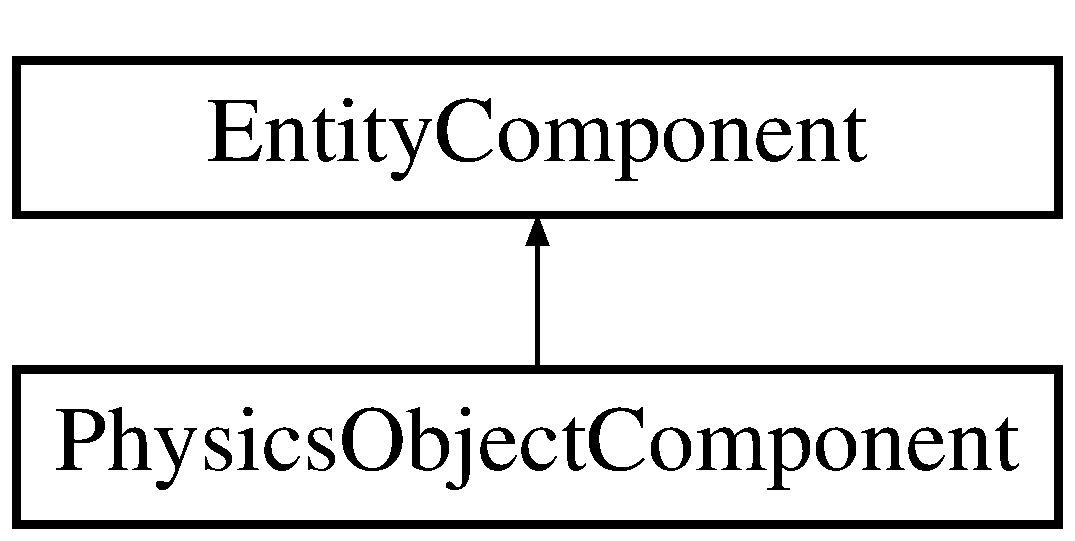
\includegraphics[height=2.000000cm]{class_entity_component}
\end{center}
\end{figure}
\subsection*{Public Member Functions}
\begin{DoxyCompactItemize}
\item 
\hyperlink{class_entity_component_a5b45c598f39fcc9237d1ab02dde89cd7}{Entity\+Component} ()
\item 
virtual \hyperlink{class_entity_component_a242864ddd9852130396e445386ae123f}{$\sim$\+Entity\+Component} ()
\item 
virtual std\+::string \hyperlink{class_entity_component_a145c9da56a1ed62e159514e14e4d8e16}{\+\_\+\+Get\+Class\+Name\+\_\+} ()
\item 
virtual void \hyperlink{class_entity_component_ae8878fb678135211d30c6ef23d8447e7}{Init} ()
\item 
virtual void \hyperlink{class_entity_component_a2145c244df8f84a1291e58bf1482a940}{Process\+Input} (const \hyperlink{class_input}{Input} \&input, float delta)
\item 
virtual void \hyperlink{class_entity_component_aa73f3be22173ada22f997825f29aa918}{Update} (float delta)
\item 
virtual void \hyperlink{class_entity_component_abb4682ad76a14bd2d3a7048eb82f3cda}{Render} (const \hyperlink{class_shader}{Shader} \&shader, const \hyperlink{class_rendering_engine}{Rendering\+Engine} \&rendering\+Engine, const \hyperlink{class_camera}{Camera} \&camera) const 
\item 
virtual void \hyperlink{class_entity_component_a43c059d7bf5a5bc1ef90c042c1bf7866}{Post\+Render} (const \hyperlink{class_shader}{Shader} \&shader, const \hyperlink{class_rendering_engine}{Rendering\+Engine} \&rendering\+Engine, const \hyperlink{class_camera}{Camera} \&camera) const 
\item 
virtual void \hyperlink{class_entity_component_a70083a6d43cc3330ee2914b446db1cf6}{Add\+To\+Engine} (\hyperlink{class_core_engine}{Core\+Engine} $\ast$engine)
\item 
\hyperlink{class_transform}{Transform} $\ast$ \hyperlink{class_entity_component_a59e8c59a5f0eda12e4702d8767757566}{Get\+Transform} ()
\item 
const \hyperlink{class_transform}{Transform} \& \hyperlink{class_entity_component_a53dffd62a15933b387a919fe4d56c9bc}{Get\+Transform} () const 
\item 
virtual void \hyperlink{class_entity_component_a99e0aca0d54b535a83f27b9a80845458}{Set\+Parent} (\hyperlink{class_entity}{Entity} $\ast$parent)
\item 
\hyperlink{class_entity}{Entity} $\ast$ \hyperlink{class_entity_component_a1f7f2527931a1ee880178e1587e997b5}{Get\+Parent} ()
\end{DoxyCompactItemize}


\subsection{Constructor \& Destructor Documentation}
\hypertarget{class_entity_component_a5b45c598f39fcc9237d1ab02dde89cd7}{}\index{Entity\+Component@{Entity\+Component}!Entity\+Component@{Entity\+Component}}
\index{Entity\+Component@{Entity\+Component}!Entity\+Component@{Entity\+Component}}
\subsubsection[{Entity\+Component()}]{\setlength{\rightskip}{0pt plus 5cm}Entity\+Component\+::\+Entity\+Component (
\begin{DoxyParamCaption}
{}
\end{DoxyParamCaption}
)\hspace{0.3cm}{\ttfamily [inline]}}\label{class_entity_component_a5b45c598f39fcc9237d1ab02dde89cd7}
\hypertarget{class_entity_component_a242864ddd9852130396e445386ae123f}{}\index{Entity\+Component@{Entity\+Component}!````~Entity\+Component@{$\sim$\+Entity\+Component}}
\index{````~Entity\+Component@{$\sim$\+Entity\+Component}!Entity\+Component@{Entity\+Component}}
\subsubsection[{$\sim$\+Entity\+Component()}]{\setlength{\rightskip}{0pt plus 5cm}virtual Entity\+Component\+::$\sim$\+Entity\+Component (
\begin{DoxyParamCaption}
{}
\end{DoxyParamCaption}
)\hspace{0.3cm}{\ttfamily [inline]}, {\ttfamily [virtual]}}\label{class_entity_component_a242864ddd9852130396e445386ae123f}


\subsection{Member Function Documentation}
\hypertarget{class_entity_component_a145c9da56a1ed62e159514e14e4d8e16}{}\index{Entity\+Component@{Entity\+Component}!\+\_\+\+Get\+Class\+Name\+\_\+@{\+\_\+\+Get\+Class\+Name\+\_\+}}
\index{\+\_\+\+Get\+Class\+Name\+\_\+@{\+\_\+\+Get\+Class\+Name\+\_\+}!Entity\+Component@{Entity\+Component}}
\subsubsection[{\+\_\+\+Get\+Class\+Name\+\_\+()}]{\setlength{\rightskip}{0pt plus 5cm}virtual std\+::string Entity\+Component\+::\+\_\+\+Get\+Class\+Name\+\_\+ (
\begin{DoxyParamCaption}
{}
\end{DoxyParamCaption}
)\hspace{0.3cm}{\ttfamily [inline]}, {\ttfamily [virtual]}}\label{class_entity_component_a145c9da56a1ed62e159514e14e4d8e16}
\hypertarget{class_entity_component_a70083a6d43cc3330ee2914b446db1cf6}{}\index{Entity\+Component@{Entity\+Component}!Add\+To\+Engine@{Add\+To\+Engine}}
\index{Add\+To\+Engine@{Add\+To\+Engine}!Entity\+Component@{Entity\+Component}}
\subsubsection[{Add\+To\+Engine(\+Core\+Engine $\ast$engine)}]{\setlength{\rightskip}{0pt plus 5cm}virtual void Entity\+Component\+::\+Add\+To\+Engine (
\begin{DoxyParamCaption}
\item[{{\bf Core\+Engine} $\ast$}]{engine}
\end{DoxyParamCaption}
)\hspace{0.3cm}{\ttfamily [inline]}, {\ttfamily [virtual]}}\label{class_entity_component_a70083a6d43cc3330ee2914b446db1cf6}
\hypertarget{class_entity_component_a1f7f2527931a1ee880178e1587e997b5}{}\index{Entity\+Component@{Entity\+Component}!Get\+Parent@{Get\+Parent}}
\index{Get\+Parent@{Get\+Parent}!Entity\+Component@{Entity\+Component}}
\subsubsection[{Get\+Parent()}]{\setlength{\rightskip}{0pt plus 5cm}{\bf Entity}$\ast$ Entity\+Component\+::\+Get\+Parent (
\begin{DoxyParamCaption}
{}
\end{DoxyParamCaption}
)\hspace{0.3cm}{\ttfamily [inline]}}\label{class_entity_component_a1f7f2527931a1ee880178e1587e997b5}
\hypertarget{class_entity_component_a59e8c59a5f0eda12e4702d8767757566}{}\index{Entity\+Component@{Entity\+Component}!Get\+Transform@{Get\+Transform}}
\index{Get\+Transform@{Get\+Transform}!Entity\+Component@{Entity\+Component}}
\subsubsection[{Get\+Transform()}]{\setlength{\rightskip}{0pt plus 5cm}{\bf Transform}$\ast$ Entity\+Component\+::\+Get\+Transform (
\begin{DoxyParamCaption}
{}
\end{DoxyParamCaption}
)\hspace{0.3cm}{\ttfamily [inline]}}\label{class_entity_component_a59e8c59a5f0eda12e4702d8767757566}
\hypertarget{class_entity_component_a53dffd62a15933b387a919fe4d56c9bc}{}\index{Entity\+Component@{Entity\+Component}!Get\+Transform@{Get\+Transform}}
\index{Get\+Transform@{Get\+Transform}!Entity\+Component@{Entity\+Component}}
\subsubsection[{Get\+Transform() const }]{\setlength{\rightskip}{0pt plus 5cm}const {\bf Transform}\& Entity\+Component\+::\+Get\+Transform (
\begin{DoxyParamCaption}
{}
\end{DoxyParamCaption}
) const\hspace{0.3cm}{\ttfamily [inline]}}\label{class_entity_component_a53dffd62a15933b387a919fe4d56c9bc}
\hypertarget{class_entity_component_ae8878fb678135211d30c6ef23d8447e7}{}\index{Entity\+Component@{Entity\+Component}!Init@{Init}}
\index{Init@{Init}!Entity\+Component@{Entity\+Component}}
\subsubsection[{Init()}]{\setlength{\rightskip}{0pt plus 5cm}virtual void Entity\+Component\+::\+Init (
\begin{DoxyParamCaption}
{}
\end{DoxyParamCaption}
)\hspace{0.3cm}{\ttfamily [inline]}, {\ttfamily [virtual]}}\label{class_entity_component_ae8878fb678135211d30c6ef23d8447e7}


Reimplemented in \hyperlink{class_physics_object_component_a9383128bd0b76d2289664053bca5c770}{Physics\+Object\+Component}.

\hypertarget{class_entity_component_a43c059d7bf5a5bc1ef90c042c1bf7866}{}\index{Entity\+Component@{Entity\+Component}!Post\+Render@{Post\+Render}}
\index{Post\+Render@{Post\+Render}!Entity\+Component@{Entity\+Component}}
\subsubsection[{Post\+Render(const Shader \&shader, const Rendering\+Engine \&rendering\+Engine, const Camera \&camera) const }]{\setlength{\rightskip}{0pt plus 5cm}virtual void Entity\+Component\+::\+Post\+Render (
\begin{DoxyParamCaption}
\item[{const {\bf Shader} \&}]{shader, }
\item[{const {\bf Rendering\+Engine} \&}]{rendering\+Engine, }
\item[{const {\bf Camera} \&}]{camera}
\end{DoxyParamCaption}
) const\hspace{0.3cm}{\ttfamily [inline]}, {\ttfamily [virtual]}}\label{class_entity_component_a43c059d7bf5a5bc1ef90c042c1bf7866}
\hypertarget{class_entity_component_a2145c244df8f84a1291e58bf1482a940}{}\index{Entity\+Component@{Entity\+Component}!Process\+Input@{Process\+Input}}
\index{Process\+Input@{Process\+Input}!Entity\+Component@{Entity\+Component}}
\subsubsection[{Process\+Input(const Input \&input, float delta)}]{\setlength{\rightskip}{0pt plus 5cm}virtual void Entity\+Component\+::\+Process\+Input (
\begin{DoxyParamCaption}
\item[{const {\bf Input} \&}]{input, }
\item[{float}]{delta}
\end{DoxyParamCaption}
)\hspace{0.3cm}{\ttfamily [inline]}, {\ttfamily [virtual]}}\label{class_entity_component_a2145c244df8f84a1291e58bf1482a940}
\hypertarget{class_entity_component_abb4682ad76a14bd2d3a7048eb82f3cda}{}\index{Entity\+Component@{Entity\+Component}!Render@{Render}}
\index{Render@{Render}!Entity\+Component@{Entity\+Component}}
\subsubsection[{Render(const Shader \&shader, const Rendering\+Engine \&rendering\+Engine, const Camera \&camera) const }]{\setlength{\rightskip}{0pt plus 5cm}virtual void Entity\+Component\+::\+Render (
\begin{DoxyParamCaption}
\item[{const {\bf Shader} \&}]{shader, }
\item[{const {\bf Rendering\+Engine} \&}]{rendering\+Engine, }
\item[{const {\bf Camera} \&}]{camera}
\end{DoxyParamCaption}
) const\hspace{0.3cm}{\ttfamily [inline]}, {\ttfamily [virtual]}}\label{class_entity_component_abb4682ad76a14bd2d3a7048eb82f3cda}
\hypertarget{class_entity_component_a99e0aca0d54b535a83f27b9a80845458}{}\index{Entity\+Component@{Entity\+Component}!Set\+Parent@{Set\+Parent}}
\index{Set\+Parent@{Set\+Parent}!Entity\+Component@{Entity\+Component}}
\subsubsection[{Set\+Parent(\+Entity $\ast$parent)}]{\setlength{\rightskip}{0pt plus 5cm}virtual void Entity\+Component\+::\+Set\+Parent (
\begin{DoxyParamCaption}
\item[{{\bf Entity} $\ast$}]{parent}
\end{DoxyParamCaption}
)\hspace{0.3cm}{\ttfamily [inline]}, {\ttfamily [virtual]}}\label{class_entity_component_a99e0aca0d54b535a83f27b9a80845458}
\hypertarget{class_entity_component_aa73f3be22173ada22f997825f29aa918}{}\index{Entity\+Component@{Entity\+Component}!Update@{Update}}
\index{Update@{Update}!Entity\+Component@{Entity\+Component}}
\subsubsection[{Update(float delta)}]{\setlength{\rightskip}{0pt plus 5cm}virtual void Entity\+Component\+::\+Update (
\begin{DoxyParamCaption}
\item[{float}]{delta}
\end{DoxyParamCaption}
)\hspace{0.3cm}{\ttfamily [inline]}, {\ttfamily [virtual]}}\label{class_entity_component_aa73f3be22173ada22f997825f29aa918}


Reimplemented in \hyperlink{class_physics_object_component_ab06a52c369ed9cef4852309a0e97fa1c}{Physics\+Object\+Component}.



The documentation for this class was generated from the following file\+:\begin{DoxyCompactItemize}
\item 
F\+:/\+Fusion3\+D\+\_\+work/src/core/\hyperlink{entity_component_8h}{entity\+Component.\+h}\end{DoxyCompactItemize}

\hypertarget{class_game}{}\section{Game Class Reference}
\label{class_game}\index{Game@{Game}}


{\ttfamily \#include $<$game.\+h$>$}

Inheritance diagram for Game\+:\begin{figure}[H]
\begin{center}
\leavevmode
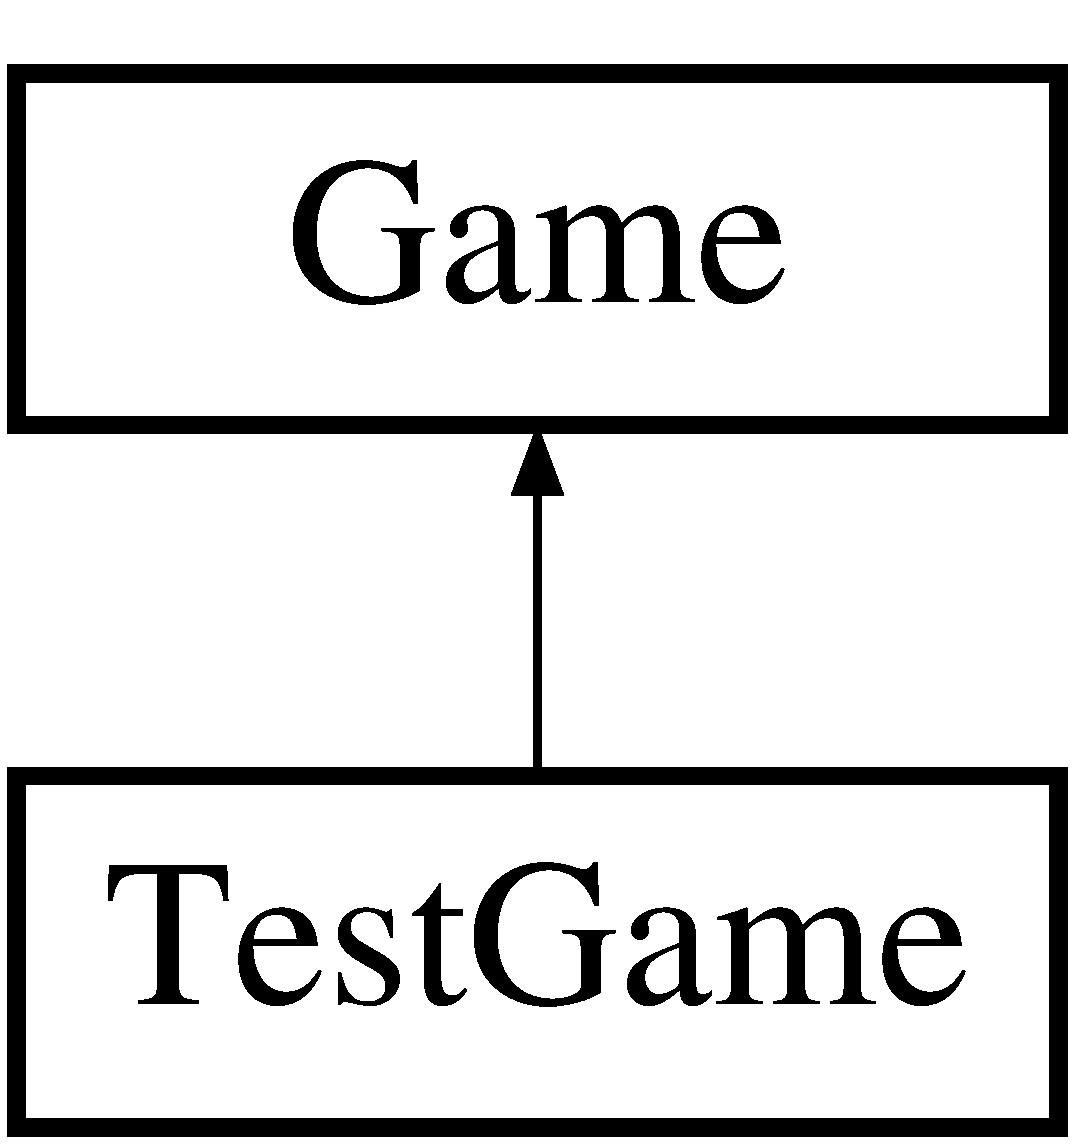
\includegraphics[height=2.000000cm]{class_game}
\end{center}
\end{figure}
\subsection*{Public Member Functions}
\begin{DoxyCompactItemize}
\item 
\hyperlink{class_game_ad59df6562a58a614fda24622d3715b65}{Game} ()
\item 
virtual \hyperlink{class_game_a72772b628443c3675976d6b5e6c9ec2a}{$\sim$\+Game} ()
\item 
virtual void \hyperlink{class_game_ad47d16f9908f7b9304bcd31db0717e0b}{Init} (const \hyperlink{class_window}{Window} \&window)
\item 
void \hyperlink{class_game_ab64891eae2c4eb4f3bf7d161c6d5e37a}{Process\+Input} (const \hyperlink{class_input}{Input} \&input, float delta)
\item 
void \hyperlink{class_game_a6ad207394e4ce91f909d49c87802da08}{Update} (float delta)
\item 
void \hyperlink{class_game_a5fae2de88740658b07d98972d4b4ed26}{Render} (\hyperlink{class_rendering_engine}{Rendering\+Engine} $\ast$rendering\+Engine)
\item 
double \hyperlink{class_game_a18483e75040298401c19befdce191aa5}{Display\+Input\+Time} (double dividend)
\item 
double \hyperlink{class_game_aec51184864470a1554fd22a47e25a0e2}{Display\+Update\+Time} (double dividend)
\item 
void \hyperlink{class_game_ab7ee30cf8ff9dd65e527b6fd1a2bd333}{Set\+Engine} (\hyperlink{class_core_engine}{Core\+Engine} $\ast$engine)
\end{DoxyCompactItemize}
\subsection*{Protected Member Functions}
\begin{DoxyCompactItemize}
\item 
\hyperlink{class_entity}{Entity} $\ast$ \hyperlink{class_game_a0b605ce1406e2afc17184221022d2075}{Add\+To\+Scene} (\hyperlink{class_entity}{Entity} $\ast$child)
\end{DoxyCompactItemize}


\subsection{Constructor \& Destructor Documentation}
\hypertarget{class_game_ad59df6562a58a614fda24622d3715b65}{}\index{Game@{Game}!Game@{Game}}
\index{Game@{Game}!Game@{Game}}
\subsubsection[{Game()}]{\setlength{\rightskip}{0pt plus 5cm}Game\+::\+Game (
\begin{DoxyParamCaption}
{}
\end{DoxyParamCaption}
)\hspace{0.3cm}{\ttfamily [inline]}}\label{class_game_ad59df6562a58a614fda24622d3715b65}
\hypertarget{class_game_a72772b628443c3675976d6b5e6c9ec2a}{}\index{Game@{Game}!````~Game@{$\sim$\+Game}}
\index{````~Game@{$\sim$\+Game}!Game@{Game}}
\subsubsection[{$\sim$\+Game()}]{\setlength{\rightskip}{0pt plus 5cm}virtual Game\+::$\sim$\+Game (
\begin{DoxyParamCaption}
{}
\end{DoxyParamCaption}
)\hspace{0.3cm}{\ttfamily [inline]}, {\ttfamily [virtual]}}\label{class_game_a72772b628443c3675976d6b5e6c9ec2a}


\subsection{Member Function Documentation}
\hypertarget{class_game_a0b605ce1406e2afc17184221022d2075}{}\index{Game@{Game}!Add\+To\+Scene@{Add\+To\+Scene}}
\index{Add\+To\+Scene@{Add\+To\+Scene}!Game@{Game}}
\subsubsection[{Add\+To\+Scene(\+Entity $\ast$child)}]{\setlength{\rightskip}{0pt plus 5cm}{\bf Entity}$\ast$ Game\+::\+Add\+To\+Scene (
\begin{DoxyParamCaption}
\item[{{\bf Entity} $\ast$}]{child}
\end{DoxyParamCaption}
)\hspace{0.3cm}{\ttfamily [inline]}, {\ttfamily [protected]}}\label{class_game_a0b605ce1406e2afc17184221022d2075}
\hypertarget{class_game_a18483e75040298401c19befdce191aa5}{}\index{Game@{Game}!Display\+Input\+Time@{Display\+Input\+Time}}
\index{Display\+Input\+Time@{Display\+Input\+Time}!Game@{Game}}
\subsubsection[{Display\+Input\+Time(double dividend)}]{\setlength{\rightskip}{0pt plus 5cm}double Game\+::\+Display\+Input\+Time (
\begin{DoxyParamCaption}
\item[{double}]{dividend}
\end{DoxyParamCaption}
)\hspace{0.3cm}{\ttfamily [inline]}}\label{class_game_a18483e75040298401c19befdce191aa5}
\hypertarget{class_game_aec51184864470a1554fd22a47e25a0e2}{}\index{Game@{Game}!Display\+Update\+Time@{Display\+Update\+Time}}
\index{Display\+Update\+Time@{Display\+Update\+Time}!Game@{Game}}
\subsubsection[{Display\+Update\+Time(double dividend)}]{\setlength{\rightskip}{0pt plus 5cm}double Game\+::\+Display\+Update\+Time (
\begin{DoxyParamCaption}
\item[{double}]{dividend}
\end{DoxyParamCaption}
)\hspace{0.3cm}{\ttfamily [inline]}}\label{class_game_aec51184864470a1554fd22a47e25a0e2}
\hypertarget{class_game_ad47d16f9908f7b9304bcd31db0717e0b}{}\index{Game@{Game}!Init@{Init}}
\index{Init@{Init}!Game@{Game}}
\subsubsection[{Init(const Window \&window)}]{\setlength{\rightskip}{0pt plus 5cm}virtual void Game\+::\+Init (
\begin{DoxyParamCaption}
\item[{const {\bf Window} \&}]{window}
\end{DoxyParamCaption}
)\hspace{0.3cm}{\ttfamily [inline]}, {\ttfamily [virtual]}}\label{class_game_ad47d16f9908f7b9304bcd31db0717e0b}


Reimplemented in \hyperlink{class_test_game_a989e3de46c3f2b0a6ff5a3fee2741489}{Test\+Game}.

\hypertarget{class_game_ab64891eae2c4eb4f3bf7d161c6d5e37a}{}\index{Game@{Game}!Process\+Input@{Process\+Input}}
\index{Process\+Input@{Process\+Input}!Game@{Game}}
\subsubsection[{Process\+Input(const Input \&input, float delta)}]{\setlength{\rightskip}{0pt plus 5cm}void Game\+::\+Process\+Input (
\begin{DoxyParamCaption}
\item[{const {\bf Input} \&}]{input, }
\item[{float}]{delta}
\end{DoxyParamCaption}
)}\label{class_game_ab64891eae2c4eb4f3bf7d161c6d5e37a}
\hypertarget{class_game_a5fae2de88740658b07d98972d4b4ed26}{}\index{Game@{Game}!Render@{Render}}
\index{Render@{Render}!Game@{Game}}
\subsubsection[{Render(\+Rendering\+Engine $\ast$rendering\+Engine)}]{\setlength{\rightskip}{0pt plus 5cm}void Game\+::\+Render (
\begin{DoxyParamCaption}
\item[{{\bf Rendering\+Engine} $\ast$}]{rendering\+Engine}
\end{DoxyParamCaption}
)}\label{class_game_a5fae2de88740658b07d98972d4b4ed26}
\hypertarget{class_game_ab7ee30cf8ff9dd65e527b6fd1a2bd333}{}\index{Game@{Game}!Set\+Engine@{Set\+Engine}}
\index{Set\+Engine@{Set\+Engine}!Game@{Game}}
\subsubsection[{Set\+Engine(\+Core\+Engine $\ast$engine)}]{\setlength{\rightskip}{0pt plus 5cm}void Game\+::\+Set\+Engine (
\begin{DoxyParamCaption}
\item[{{\bf Core\+Engine} $\ast$}]{engine}
\end{DoxyParamCaption}
)\hspace{0.3cm}{\ttfamily [inline]}}\label{class_game_ab7ee30cf8ff9dd65e527b6fd1a2bd333}
\hypertarget{class_game_a6ad207394e4ce91f909d49c87802da08}{}\index{Game@{Game}!Update@{Update}}
\index{Update@{Update}!Game@{Game}}
\subsubsection[{Update(float delta)}]{\setlength{\rightskip}{0pt plus 5cm}void Game\+::\+Update (
\begin{DoxyParamCaption}
\item[{float}]{delta}
\end{DoxyParamCaption}
)}\label{class_game_a6ad207394e4ce91f909d49c87802da08}


The documentation for this class was generated from the following files\+:\begin{DoxyCompactItemize}
\item 
F\+:/\+Fusion3\+D\+\_\+work/src/core/\hyperlink{game_8h}{game.\+h}\item 
F\+:/\+Fusion3\+D\+\_\+work/src/core/\hyperlink{game_8cpp}{game.\+cpp}\end{DoxyCompactItemize}

\hypertarget{class_g_l_debug_drawer}{}\section{G\+L\+Debug\+Drawer Class Reference}
\label{class_g_l_debug_drawer}\index{G\+L\+Debug\+Drawer@{G\+L\+Debug\+Drawer}}


{\ttfamily \#include $<$rendering\+Engine.\+h$>$}

Inheritance diagram for G\+L\+Debug\+Drawer\+:\begin{figure}[H]
\begin{center}
\leavevmode
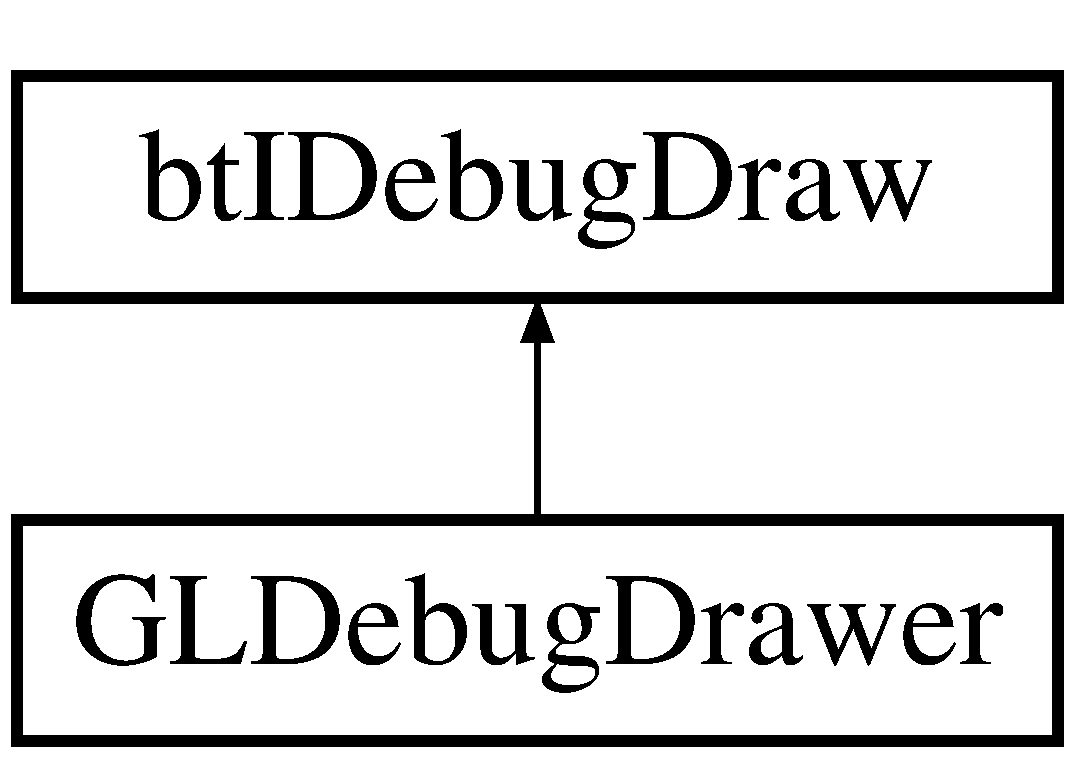
\includegraphics[height=2.000000cm]{class_g_l_debug_drawer}
\end{center}
\end{figure}
\subsection*{Public Member Functions}
\begin{DoxyCompactItemize}
\item 
\hyperlink{class_g_l_debug_drawer_abb8d86c1187b073736b72c45c748a552}{G\+L\+Debug\+Drawer} ()
\item 
virtual void \hyperlink{class_g_l_debug_drawer_a4f37715bd5fbec4eae17285bcd3024ad}{draw\+Line} (const bt\+Vector3 \&from, const bt\+Vector3 \&to, const bt\+Vector3 \&color)
\item 
virtual void \hyperlink{class_g_l_debug_drawer_aa2373d114bd57438ae3eb7319d6052f2}{draw\+Contact\+Point} (const bt\+Vector3 \&Point\+On\+B, const bt\+Vector3 \&normal\+On\+B, bt\+Scalar distance, int life\+Time, const bt\+Vector3 \&color)
\item 
virtual void \hyperlink{class_g_l_debug_drawer_a4bd03c9b18d0359dfd6d3e9450e327f8}{report\+Error\+Warning} (const char $\ast$warning\+String)
\item 
virtual void \hyperlink{class_g_l_debug_drawer_a6325861596594c1f8df946cef3d14194}{draw3d\+Text} (const bt\+Vector3 \&location, const char $\ast$text\+String)
\item 
virtual void \hyperlink{class_g_l_debug_drawer_a91f3d38a8253603e41f8a9148f37dd9a}{set\+Debug\+Mode} (int debug\+Mode)
\item 
virtual int \hyperlink{class_g_l_debug_drawer_a54af9866c8b723c08b961cf2e7905481}{get\+Debug\+Mode} () const 
\end{DoxyCompactItemize}


\subsection{Constructor \& Destructor Documentation}
\hypertarget{class_g_l_debug_drawer_abb8d86c1187b073736b72c45c748a552}{}\index{G\+L\+Debug\+Drawer@{G\+L\+Debug\+Drawer}!G\+L\+Debug\+Drawer@{G\+L\+Debug\+Drawer}}
\index{G\+L\+Debug\+Drawer@{G\+L\+Debug\+Drawer}!G\+L\+Debug\+Drawer@{G\+L\+Debug\+Drawer}}
\subsubsection[{G\+L\+Debug\+Drawer()}]{\setlength{\rightskip}{0pt plus 5cm}G\+L\+Debug\+Drawer\+::\+G\+L\+Debug\+Drawer (
\begin{DoxyParamCaption}
{}
\end{DoxyParamCaption}
)}\label{class_g_l_debug_drawer_abb8d86c1187b073736b72c45c748a552}


\subsection{Member Function Documentation}
\hypertarget{class_g_l_debug_drawer_a6325861596594c1f8df946cef3d14194}{}\index{G\+L\+Debug\+Drawer@{G\+L\+Debug\+Drawer}!draw3d\+Text@{draw3d\+Text}}
\index{draw3d\+Text@{draw3d\+Text}!G\+L\+Debug\+Drawer@{G\+L\+Debug\+Drawer}}
\subsubsection[{draw3d\+Text(const bt\+Vector3 \&location, const char $\ast$text\+String)}]{\setlength{\rightskip}{0pt plus 5cm}void G\+L\+Debug\+Drawer\+::draw3d\+Text (
\begin{DoxyParamCaption}
\item[{const bt\+Vector3 \&}]{location, }
\item[{const char $\ast$}]{text\+String}
\end{DoxyParamCaption}
)\hspace{0.3cm}{\ttfamily [virtual]}}\label{class_g_l_debug_drawer_a6325861596594c1f8df946cef3d14194}
\hypertarget{class_g_l_debug_drawer_aa2373d114bd57438ae3eb7319d6052f2}{}\index{G\+L\+Debug\+Drawer@{G\+L\+Debug\+Drawer}!draw\+Contact\+Point@{draw\+Contact\+Point}}
\index{draw\+Contact\+Point@{draw\+Contact\+Point}!G\+L\+Debug\+Drawer@{G\+L\+Debug\+Drawer}}
\subsubsection[{draw\+Contact\+Point(const bt\+Vector3 \&\+Point\+On\+B, const bt\+Vector3 \&normal\+On\+B, bt\+Scalar distance, int life\+Time, const bt\+Vector3 \&color)}]{\setlength{\rightskip}{0pt plus 5cm}void G\+L\+Debug\+Drawer\+::draw\+Contact\+Point (
\begin{DoxyParamCaption}
\item[{const bt\+Vector3 \&}]{Point\+On\+B, }
\item[{const bt\+Vector3 \&}]{normal\+On\+B, }
\item[{bt\+Scalar}]{distance, }
\item[{int}]{life\+Time, }
\item[{const bt\+Vector3 \&}]{color}
\end{DoxyParamCaption}
)\hspace{0.3cm}{\ttfamily [virtual]}}\label{class_g_l_debug_drawer_aa2373d114bd57438ae3eb7319d6052f2}
\hypertarget{class_g_l_debug_drawer_a4f37715bd5fbec4eae17285bcd3024ad}{}\index{G\+L\+Debug\+Drawer@{G\+L\+Debug\+Drawer}!draw\+Line@{draw\+Line}}
\index{draw\+Line@{draw\+Line}!G\+L\+Debug\+Drawer@{G\+L\+Debug\+Drawer}}
\subsubsection[{draw\+Line(const bt\+Vector3 \&from, const bt\+Vector3 \&to, const bt\+Vector3 \&color)}]{\setlength{\rightskip}{0pt plus 5cm}void G\+L\+Debug\+Drawer\+::draw\+Line (
\begin{DoxyParamCaption}
\item[{const bt\+Vector3 \&}]{from, }
\item[{const bt\+Vector3 \&}]{to, }
\item[{const bt\+Vector3 \&}]{color}
\end{DoxyParamCaption}
)\hspace{0.3cm}{\ttfamily [virtual]}}\label{class_g_l_debug_drawer_a4f37715bd5fbec4eae17285bcd3024ad}
\hypertarget{class_g_l_debug_drawer_a54af9866c8b723c08b961cf2e7905481}{}\index{G\+L\+Debug\+Drawer@{G\+L\+Debug\+Drawer}!get\+Debug\+Mode@{get\+Debug\+Mode}}
\index{get\+Debug\+Mode@{get\+Debug\+Mode}!G\+L\+Debug\+Drawer@{G\+L\+Debug\+Drawer}}
\subsubsection[{get\+Debug\+Mode() const }]{\setlength{\rightskip}{0pt plus 5cm}virtual int G\+L\+Debug\+Drawer\+::get\+Debug\+Mode (
\begin{DoxyParamCaption}
{}
\end{DoxyParamCaption}
) const\hspace{0.3cm}{\ttfamily [inline]}, {\ttfamily [virtual]}}\label{class_g_l_debug_drawer_a54af9866c8b723c08b961cf2e7905481}
\hypertarget{class_g_l_debug_drawer_a4bd03c9b18d0359dfd6d3e9450e327f8}{}\index{G\+L\+Debug\+Drawer@{G\+L\+Debug\+Drawer}!report\+Error\+Warning@{report\+Error\+Warning}}
\index{report\+Error\+Warning@{report\+Error\+Warning}!G\+L\+Debug\+Drawer@{G\+L\+Debug\+Drawer}}
\subsubsection[{report\+Error\+Warning(const char $\ast$warning\+String)}]{\setlength{\rightskip}{0pt plus 5cm}void G\+L\+Debug\+Drawer\+::report\+Error\+Warning (
\begin{DoxyParamCaption}
\item[{const char $\ast$}]{warning\+String}
\end{DoxyParamCaption}
)\hspace{0.3cm}{\ttfamily [virtual]}}\label{class_g_l_debug_drawer_a4bd03c9b18d0359dfd6d3e9450e327f8}
\hypertarget{class_g_l_debug_drawer_a91f3d38a8253603e41f8a9148f37dd9a}{}\index{G\+L\+Debug\+Drawer@{G\+L\+Debug\+Drawer}!set\+Debug\+Mode@{set\+Debug\+Mode}}
\index{set\+Debug\+Mode@{set\+Debug\+Mode}!G\+L\+Debug\+Drawer@{G\+L\+Debug\+Drawer}}
\subsubsection[{set\+Debug\+Mode(int debug\+Mode)}]{\setlength{\rightskip}{0pt plus 5cm}void G\+L\+Debug\+Drawer\+::set\+Debug\+Mode (
\begin{DoxyParamCaption}
\item[{int}]{debug\+Mode}
\end{DoxyParamCaption}
)\hspace{0.3cm}{\ttfamily [virtual]}}\label{class_g_l_debug_drawer_a91f3d38a8253603e41f8a9148f37dd9a}


The documentation for this class was generated from the following files\+:\begin{DoxyCompactItemize}
\item 
F\+:/\+Fusion3\+D\+\_\+work/src/rendering/\hyperlink{rendering_engine_8h}{rendering\+Engine.\+h}\item 
F\+:/\+Fusion3\+D\+\_\+work/src/rendering/\hyperlink{rendering_engine_8cpp}{rendering\+Engine.\+cpp}\end{DoxyCompactItemize}

\hypertarget{structhuffman}{}\section{huffman Struct Reference}
\label{structhuffman}\index{huffman@{huffman}}
\subsection*{Public Attributes}
\begin{DoxyCompactItemize}
\item 
\hyperlink{stb__image_8c_adde6aaee8457bee49c2a92621fe22b79}{uint8} \hyperlink{structhuffman_a9dbb29a8ed724a32f502d9595510ddc2}{fast} \mbox{[}1$<$$<$ \hyperlink{stb__image_8c_add78822c51f4692289f2ce174bdf82b0}{F\+A\+S\+T\+\_\+\+B\+I\+T\+S}\mbox{]}
\item 
\hyperlink{stb__image_8c_a05f6b0ae8f6a6e135b0e290c25fe0e4e}{uint16} \hyperlink{structhuffman_a9925018a95d5a2122cd732561fa0fa64}{code} \mbox{[}256\mbox{]}
\item 
\hyperlink{stb__image_8c_adde6aaee8457bee49c2a92621fe22b79}{uint8} \hyperlink{structhuffman_a313d78cf23f40b314c25681ff2a6224b}{values} \mbox{[}256\mbox{]}
\item 
\hyperlink{stb__image_8c_adde6aaee8457bee49c2a92621fe22b79}{uint8} \hyperlink{structhuffman_afdb0fbcf25aec42ba30b0d0e2453a057}{size} \mbox{[}257\mbox{]}
\item 
unsigned int \hyperlink{structhuffman_aeb78aca6c7377faaad8123566d54fc98}{maxcode} \mbox{[}18\mbox{]}
\item 
int \hyperlink{structhuffman_a04255e3e1c6de74d36a08a1aa4e9537d}{delta} \mbox{[}17\mbox{]}
\end{DoxyCompactItemize}


\subsection{Member Data Documentation}
\hypertarget{structhuffman_a9925018a95d5a2122cd732561fa0fa64}{}\index{huffman@{huffman}!code@{code}}
\index{code@{code}!huffman@{huffman}}
\subsubsection[{code}]{\setlength{\rightskip}{0pt plus 5cm}{\bf uint16} huffman\+::code\mbox{[}256\mbox{]}}\label{structhuffman_a9925018a95d5a2122cd732561fa0fa64}
\hypertarget{structhuffman_a04255e3e1c6de74d36a08a1aa4e9537d}{}\index{huffman@{huffman}!delta@{delta}}
\index{delta@{delta}!huffman@{huffman}}
\subsubsection[{delta}]{\setlength{\rightskip}{0pt plus 5cm}int huffman\+::delta\mbox{[}17\mbox{]}}\label{structhuffman_a04255e3e1c6de74d36a08a1aa4e9537d}
\hypertarget{structhuffman_a9dbb29a8ed724a32f502d9595510ddc2}{}\index{huffman@{huffman}!fast@{fast}}
\index{fast@{fast}!huffman@{huffman}}
\subsubsection[{fast}]{\setlength{\rightskip}{0pt plus 5cm}{\bf uint8} huffman\+::fast\mbox{[}1$<$$<$ {\bf F\+A\+S\+T\+\_\+\+B\+I\+T\+S}\mbox{]}}\label{structhuffman_a9dbb29a8ed724a32f502d9595510ddc2}
\hypertarget{structhuffman_aeb78aca6c7377faaad8123566d54fc98}{}\index{huffman@{huffman}!maxcode@{maxcode}}
\index{maxcode@{maxcode}!huffman@{huffman}}
\subsubsection[{maxcode}]{\setlength{\rightskip}{0pt plus 5cm}unsigned int huffman\+::maxcode\mbox{[}18\mbox{]}}\label{structhuffman_aeb78aca6c7377faaad8123566d54fc98}
\hypertarget{structhuffman_afdb0fbcf25aec42ba30b0d0e2453a057}{}\index{huffman@{huffman}!size@{size}}
\index{size@{size}!huffman@{huffman}}
\subsubsection[{size}]{\setlength{\rightskip}{0pt plus 5cm}{\bf uint8} huffman\+::size\mbox{[}257\mbox{]}}\label{structhuffman_afdb0fbcf25aec42ba30b0d0e2453a057}
\hypertarget{structhuffman_a313d78cf23f40b314c25681ff2a6224b}{}\index{huffman@{huffman}!values@{values}}
\index{values@{values}!huffman@{huffman}}
\subsubsection[{values}]{\setlength{\rightskip}{0pt plus 5cm}{\bf uint8} huffman\+::values\mbox{[}256\mbox{]}}\label{structhuffman_a313d78cf23f40b314c25681ff2a6224b}


The documentation for this struct was generated from the following file\+:\begin{DoxyCompactItemize}
\item 
F\+:/\+Fusion3\+D\+\_\+work/src/static\+Libs/\hyperlink{stb__image_8c}{stb\+\_\+image.\+c}\end{DoxyCompactItemize}

\hypertarget{class_indexed_model}{}\section{Indexed\+Model Class Reference}
\label{class_indexed_model}\index{Indexed\+Model@{Indexed\+Model}}


{\ttfamily \#include $<$mesh.\+h$>$}

\subsection*{Public Member Functions}
\begin{DoxyCompactItemize}
\item 
\hyperlink{class_indexed_model_a1e547725f750214d5d4478ae5dda27fd}{Indexed\+Model} ()
\item 
\hyperlink{class_indexed_model_ad3927c4cd998510c27b6d78d453eed8c}{Indexed\+Model} (const std\+::vector$<$ unsigned int $>$ indices, const std\+::vector$<$ \hyperlink{class_vector3f}{Vector3f} $>$ \&positions, const std\+::vector$<$ \hyperlink{math3d_8h_a9f3739462b0605dcb64299fa289b6afe}{Vector2f} $>$ \&tex\+Coords, const std\+::vector$<$ \hyperlink{class_vector3f}{Vector3f} $>$ \&normals=std\+::vector$<$ \hyperlink{class_vector3f}{Vector3f} $>$(), const std\+::vector$<$ \hyperlink{class_vector3f}{Vector3f} $>$ \&tangents=std\+::vector$<$ \hyperlink{class_vector3f}{Vector3f} $>$())
\item 
bool \hyperlink{class_indexed_model_adbca8c4691184cfaff137d228ddd885c}{Is\+Valid} () const 
\item 
void \hyperlink{class_indexed_model_ad7c6f8680a079108e64d463b34dca802}{Calc\+Normals} ()
\item 
void \hyperlink{class_indexed_model_a5d9194a38c4c18cf5159d7fe5dbd1e14}{Calc\+Tangents} ()
\item 
\hyperlink{class_indexed_model}{Indexed\+Model} \hyperlink{class_indexed_model_a8f39e2fa52afdcfc5637487a37625a36}{Finalize} ()
\item 
void \hyperlink{class_indexed_model_a12ffb5465a583451ae594741a7151503}{Add\+Vertex} (const \hyperlink{class_vector3f}{Vector3f} \&vert)
\item 
void \hyperlink{class_indexed_model_af9e4cf11a7382e12d0d190f68f2a0549}{Add\+Vertex} (float x, float y, float z)
\item 
void \hyperlink{class_indexed_model_a8e64a560d6421b5208426e82bca89bc2}{Add\+Tex\+Coord} (const \hyperlink{math3d_8h_a9f3739462b0605dcb64299fa289b6afe}{Vector2f} \&tex\+Coord)
\item 
void \hyperlink{class_indexed_model_a21da70d87dce12969ef9f4ececc1f457}{Add\+Tex\+Coord} (float x, float y)
\item 
void \hyperlink{class_indexed_model_a5234351972aff54068ccda7054005529}{Add\+Normal} (const \hyperlink{class_vector3f}{Vector3f} \&normal)
\item 
void \hyperlink{class_indexed_model_adffa79edb321e84b2c73cd85d65369a8}{Add\+Normal} (float x, float y, float z)
\item 
void \hyperlink{class_indexed_model_ac409f2c18136e1c5669de9782c50a452}{Add\+Tangent} (const \hyperlink{class_vector3f}{Vector3f} \&tangent)
\item 
void \hyperlink{class_indexed_model_a6a2c1ce5e751a824ba962189332bf79c}{Add\+Tangent} (float x, float y, float z)
\item 
void \hyperlink{class_indexed_model_a76422df31bb87d55fadbd5baff70c331}{Add\+Face} (unsigned int vert\+Index0, unsigned int vert\+Index1, unsigned int vert\+Index2)
\item 
const std\+::vector$<$ unsigned int $>$ \& \hyperlink{class_indexed_model_a95bc43f2719df501d635987a3ffbbbca}{Get\+Indices} () const 
\item 
const std\+::vector$<$ \hyperlink{class_vector3f}{Vector3f} $>$ \& \hyperlink{class_indexed_model_a82cdd0a943892e1dea0657c1c58f1ee2}{Get\+Positions} () const 
\item 
const std\+::vector$<$ \hyperlink{math3d_8h_a9f3739462b0605dcb64299fa289b6afe}{Vector2f} $>$ \& \hyperlink{class_indexed_model_abf332c063e230c66895129fe7b8f7d8a}{Get\+Tex\+Coords} () const 
\item 
const std\+::vector$<$ \hyperlink{class_vector3f}{Vector3f} $>$ \& \hyperlink{class_indexed_model_a01877af59d10674f69517745d9fc04bf}{Get\+Normals} () const 
\item 
const std\+::vector$<$ \hyperlink{class_vector3f}{Vector3f} $>$ \& \hyperlink{class_indexed_model_a03d5a41eec38962b9eb3a34cbe7732ab}{Get\+Tangents} () const 
\end{DoxyCompactItemize}


\subsection{Constructor \& Destructor Documentation}
\hypertarget{class_indexed_model_a1e547725f750214d5d4478ae5dda27fd}{}\index{Indexed\+Model@{Indexed\+Model}!Indexed\+Model@{Indexed\+Model}}
\index{Indexed\+Model@{Indexed\+Model}!Indexed\+Model@{Indexed\+Model}}
\subsubsection[{Indexed\+Model()}]{\setlength{\rightskip}{0pt plus 5cm}Indexed\+Model\+::\+Indexed\+Model (
\begin{DoxyParamCaption}
{}
\end{DoxyParamCaption}
)\hspace{0.3cm}{\ttfamily [inline]}}\label{class_indexed_model_a1e547725f750214d5d4478ae5dda27fd}
\hypertarget{class_indexed_model_ad3927c4cd998510c27b6d78d453eed8c}{}\index{Indexed\+Model@{Indexed\+Model}!Indexed\+Model@{Indexed\+Model}}
\index{Indexed\+Model@{Indexed\+Model}!Indexed\+Model@{Indexed\+Model}}
\subsubsection[{Indexed\+Model(const std\+::vector$<$ unsigned int $>$ indices, const std\+::vector$<$ Vector3f $>$ \&positions, const std\+::vector$<$ Vector2f $>$ \&tex\+Coords, const std\+::vector$<$ Vector3f $>$ \&normals=std\+::vector$<$ Vector3f $>$(), const std\+::vector$<$ Vector3f $>$ \&tangents=std\+::vector$<$ Vector3f $>$())}]{\setlength{\rightskip}{0pt plus 5cm}Indexed\+Model\+::\+Indexed\+Model (
\begin{DoxyParamCaption}
\item[{const std\+::vector$<$ unsigned int $>$}]{indices, }
\item[{const std\+::vector$<$ {\bf Vector3f} $>$ \&}]{positions, }
\item[{const std\+::vector$<$ {\bf Vector2f} $>$ \&}]{tex\+Coords, }
\item[{const std\+::vector$<$ {\bf Vector3f} $>$ \&}]{normals = {\ttfamily std\+:\+:vector$<${\bf Vector3f}$>$()}, }
\item[{const std\+::vector$<$ {\bf Vector3f} $>$ \&}]{tangents = {\ttfamily std\+:\+:vector$<${\bf Vector3f}$>$()}}
\end{DoxyParamCaption}
)\hspace{0.3cm}{\ttfamily [inline]}}\label{class_indexed_model_ad3927c4cd998510c27b6d78d453eed8c}


\subsection{Member Function Documentation}
\hypertarget{class_indexed_model_a76422df31bb87d55fadbd5baff70c331}{}\index{Indexed\+Model@{Indexed\+Model}!Add\+Face@{Add\+Face}}
\index{Add\+Face@{Add\+Face}!Indexed\+Model@{Indexed\+Model}}
\subsubsection[{Add\+Face(unsigned int vert\+Index0, unsigned int vert\+Index1, unsigned int vert\+Index2)}]{\setlength{\rightskip}{0pt plus 5cm}void Indexed\+Model\+::\+Add\+Face (
\begin{DoxyParamCaption}
\item[{unsigned int}]{vert\+Index0, }
\item[{unsigned int}]{vert\+Index1, }
\item[{unsigned int}]{vert\+Index2}
\end{DoxyParamCaption}
)}\label{class_indexed_model_a76422df31bb87d55fadbd5baff70c331}
\hypertarget{class_indexed_model_a5234351972aff54068ccda7054005529}{}\index{Indexed\+Model@{Indexed\+Model}!Add\+Normal@{Add\+Normal}}
\index{Add\+Normal@{Add\+Normal}!Indexed\+Model@{Indexed\+Model}}
\subsubsection[{Add\+Normal(const Vector3f \&normal)}]{\setlength{\rightskip}{0pt plus 5cm}void Indexed\+Model\+::\+Add\+Normal (
\begin{DoxyParamCaption}
\item[{const {\bf Vector3f} \&}]{normal}
\end{DoxyParamCaption}
)}\label{class_indexed_model_a5234351972aff54068ccda7054005529}
\hypertarget{class_indexed_model_adffa79edb321e84b2c73cd85d65369a8}{}\index{Indexed\+Model@{Indexed\+Model}!Add\+Normal@{Add\+Normal}}
\index{Add\+Normal@{Add\+Normal}!Indexed\+Model@{Indexed\+Model}}
\subsubsection[{Add\+Normal(float x, float y, float z)}]{\setlength{\rightskip}{0pt plus 5cm}void Indexed\+Model\+::\+Add\+Normal (
\begin{DoxyParamCaption}
\item[{float}]{x, }
\item[{float}]{y, }
\item[{float}]{z}
\end{DoxyParamCaption}
)\hspace{0.3cm}{\ttfamily [inline]}}\label{class_indexed_model_adffa79edb321e84b2c73cd85d65369a8}
\hypertarget{class_indexed_model_ac409f2c18136e1c5669de9782c50a452}{}\index{Indexed\+Model@{Indexed\+Model}!Add\+Tangent@{Add\+Tangent}}
\index{Add\+Tangent@{Add\+Tangent}!Indexed\+Model@{Indexed\+Model}}
\subsubsection[{Add\+Tangent(const Vector3f \&tangent)}]{\setlength{\rightskip}{0pt plus 5cm}void Indexed\+Model\+::\+Add\+Tangent (
\begin{DoxyParamCaption}
\item[{const {\bf Vector3f} \&}]{tangent}
\end{DoxyParamCaption}
)}\label{class_indexed_model_ac409f2c18136e1c5669de9782c50a452}
\hypertarget{class_indexed_model_a6a2c1ce5e751a824ba962189332bf79c}{}\index{Indexed\+Model@{Indexed\+Model}!Add\+Tangent@{Add\+Tangent}}
\index{Add\+Tangent@{Add\+Tangent}!Indexed\+Model@{Indexed\+Model}}
\subsubsection[{Add\+Tangent(float x, float y, float z)}]{\setlength{\rightskip}{0pt plus 5cm}void Indexed\+Model\+::\+Add\+Tangent (
\begin{DoxyParamCaption}
\item[{float}]{x, }
\item[{float}]{y, }
\item[{float}]{z}
\end{DoxyParamCaption}
)\hspace{0.3cm}{\ttfamily [inline]}}\label{class_indexed_model_a6a2c1ce5e751a824ba962189332bf79c}
\hypertarget{class_indexed_model_a8e64a560d6421b5208426e82bca89bc2}{}\index{Indexed\+Model@{Indexed\+Model}!Add\+Tex\+Coord@{Add\+Tex\+Coord}}
\index{Add\+Tex\+Coord@{Add\+Tex\+Coord}!Indexed\+Model@{Indexed\+Model}}
\subsubsection[{Add\+Tex\+Coord(const Vector2f \&tex\+Coord)}]{\setlength{\rightskip}{0pt plus 5cm}void Indexed\+Model\+::\+Add\+Tex\+Coord (
\begin{DoxyParamCaption}
\item[{const {\bf Vector2f} \&}]{tex\+Coord}
\end{DoxyParamCaption}
)}\label{class_indexed_model_a8e64a560d6421b5208426e82bca89bc2}
\hypertarget{class_indexed_model_a21da70d87dce12969ef9f4ececc1f457}{}\index{Indexed\+Model@{Indexed\+Model}!Add\+Tex\+Coord@{Add\+Tex\+Coord}}
\index{Add\+Tex\+Coord@{Add\+Tex\+Coord}!Indexed\+Model@{Indexed\+Model}}
\subsubsection[{Add\+Tex\+Coord(float x, float y)}]{\setlength{\rightskip}{0pt plus 5cm}void Indexed\+Model\+::\+Add\+Tex\+Coord (
\begin{DoxyParamCaption}
\item[{float}]{x, }
\item[{float}]{y}
\end{DoxyParamCaption}
)\hspace{0.3cm}{\ttfamily [inline]}}\label{class_indexed_model_a21da70d87dce12969ef9f4ececc1f457}
\hypertarget{class_indexed_model_a12ffb5465a583451ae594741a7151503}{}\index{Indexed\+Model@{Indexed\+Model}!Add\+Vertex@{Add\+Vertex}}
\index{Add\+Vertex@{Add\+Vertex}!Indexed\+Model@{Indexed\+Model}}
\subsubsection[{Add\+Vertex(const Vector3f \&vert)}]{\setlength{\rightskip}{0pt plus 5cm}void Indexed\+Model\+::\+Add\+Vertex (
\begin{DoxyParamCaption}
\item[{const {\bf Vector3f} \&}]{vert}
\end{DoxyParamCaption}
)}\label{class_indexed_model_a12ffb5465a583451ae594741a7151503}
\hypertarget{class_indexed_model_af9e4cf11a7382e12d0d190f68f2a0549}{}\index{Indexed\+Model@{Indexed\+Model}!Add\+Vertex@{Add\+Vertex}}
\index{Add\+Vertex@{Add\+Vertex}!Indexed\+Model@{Indexed\+Model}}
\subsubsection[{Add\+Vertex(float x, float y, float z)}]{\setlength{\rightskip}{0pt plus 5cm}void Indexed\+Model\+::\+Add\+Vertex (
\begin{DoxyParamCaption}
\item[{float}]{x, }
\item[{float}]{y, }
\item[{float}]{z}
\end{DoxyParamCaption}
)\hspace{0.3cm}{\ttfamily [inline]}}\label{class_indexed_model_af9e4cf11a7382e12d0d190f68f2a0549}
\hypertarget{class_indexed_model_ad7c6f8680a079108e64d463b34dca802}{}\index{Indexed\+Model@{Indexed\+Model}!Calc\+Normals@{Calc\+Normals}}
\index{Calc\+Normals@{Calc\+Normals}!Indexed\+Model@{Indexed\+Model}}
\subsubsection[{Calc\+Normals()}]{\setlength{\rightskip}{0pt plus 5cm}void Indexed\+Model\+::\+Calc\+Normals (
\begin{DoxyParamCaption}
{}
\end{DoxyParamCaption}
)}\label{class_indexed_model_ad7c6f8680a079108e64d463b34dca802}
\hypertarget{class_indexed_model_a5d9194a38c4c18cf5159d7fe5dbd1e14}{}\index{Indexed\+Model@{Indexed\+Model}!Calc\+Tangents@{Calc\+Tangents}}
\index{Calc\+Tangents@{Calc\+Tangents}!Indexed\+Model@{Indexed\+Model}}
\subsubsection[{Calc\+Tangents()}]{\setlength{\rightskip}{0pt plus 5cm}void Indexed\+Model\+::\+Calc\+Tangents (
\begin{DoxyParamCaption}
{}
\end{DoxyParamCaption}
)}\label{class_indexed_model_a5d9194a38c4c18cf5159d7fe5dbd1e14}
\hypertarget{class_indexed_model_a8f39e2fa52afdcfc5637487a37625a36}{}\index{Indexed\+Model@{Indexed\+Model}!Finalize@{Finalize}}
\index{Finalize@{Finalize}!Indexed\+Model@{Indexed\+Model}}
\subsubsection[{Finalize()}]{\setlength{\rightskip}{0pt plus 5cm}{\bf Indexed\+Model} Indexed\+Model\+::\+Finalize (
\begin{DoxyParamCaption}
{}
\end{DoxyParamCaption}
)}\label{class_indexed_model_a8f39e2fa52afdcfc5637487a37625a36}
\hypertarget{class_indexed_model_a95bc43f2719df501d635987a3ffbbbca}{}\index{Indexed\+Model@{Indexed\+Model}!Get\+Indices@{Get\+Indices}}
\index{Get\+Indices@{Get\+Indices}!Indexed\+Model@{Indexed\+Model}}
\subsubsection[{Get\+Indices() const }]{\setlength{\rightskip}{0pt plus 5cm}const std\+::vector$<$unsigned int$>$\& Indexed\+Model\+::\+Get\+Indices (
\begin{DoxyParamCaption}
{}
\end{DoxyParamCaption}
) const\hspace{0.3cm}{\ttfamily [inline]}}\label{class_indexed_model_a95bc43f2719df501d635987a3ffbbbca}
\hypertarget{class_indexed_model_a01877af59d10674f69517745d9fc04bf}{}\index{Indexed\+Model@{Indexed\+Model}!Get\+Normals@{Get\+Normals}}
\index{Get\+Normals@{Get\+Normals}!Indexed\+Model@{Indexed\+Model}}
\subsubsection[{Get\+Normals() const }]{\setlength{\rightskip}{0pt plus 5cm}const std\+::vector$<${\bf Vector3f}$>$\& Indexed\+Model\+::\+Get\+Normals (
\begin{DoxyParamCaption}
{}
\end{DoxyParamCaption}
) const\hspace{0.3cm}{\ttfamily [inline]}}\label{class_indexed_model_a01877af59d10674f69517745d9fc04bf}
\hypertarget{class_indexed_model_a82cdd0a943892e1dea0657c1c58f1ee2}{}\index{Indexed\+Model@{Indexed\+Model}!Get\+Positions@{Get\+Positions}}
\index{Get\+Positions@{Get\+Positions}!Indexed\+Model@{Indexed\+Model}}
\subsubsection[{Get\+Positions() const }]{\setlength{\rightskip}{0pt plus 5cm}const std\+::vector$<${\bf Vector3f}$>$\& Indexed\+Model\+::\+Get\+Positions (
\begin{DoxyParamCaption}
{}
\end{DoxyParamCaption}
) const\hspace{0.3cm}{\ttfamily [inline]}}\label{class_indexed_model_a82cdd0a943892e1dea0657c1c58f1ee2}
\hypertarget{class_indexed_model_a03d5a41eec38962b9eb3a34cbe7732ab}{}\index{Indexed\+Model@{Indexed\+Model}!Get\+Tangents@{Get\+Tangents}}
\index{Get\+Tangents@{Get\+Tangents}!Indexed\+Model@{Indexed\+Model}}
\subsubsection[{Get\+Tangents() const }]{\setlength{\rightskip}{0pt plus 5cm}const std\+::vector$<${\bf Vector3f}$>$\& Indexed\+Model\+::\+Get\+Tangents (
\begin{DoxyParamCaption}
{}
\end{DoxyParamCaption}
) const\hspace{0.3cm}{\ttfamily [inline]}}\label{class_indexed_model_a03d5a41eec38962b9eb3a34cbe7732ab}
\hypertarget{class_indexed_model_abf332c063e230c66895129fe7b8f7d8a}{}\index{Indexed\+Model@{Indexed\+Model}!Get\+Tex\+Coords@{Get\+Tex\+Coords}}
\index{Get\+Tex\+Coords@{Get\+Tex\+Coords}!Indexed\+Model@{Indexed\+Model}}
\subsubsection[{Get\+Tex\+Coords() const }]{\setlength{\rightskip}{0pt plus 5cm}const std\+::vector$<${\bf Vector2f}$>$\& Indexed\+Model\+::\+Get\+Tex\+Coords (
\begin{DoxyParamCaption}
{}
\end{DoxyParamCaption}
) const\hspace{0.3cm}{\ttfamily [inline]}}\label{class_indexed_model_abf332c063e230c66895129fe7b8f7d8a}
\hypertarget{class_indexed_model_adbca8c4691184cfaff137d228ddd885c}{}\index{Indexed\+Model@{Indexed\+Model}!Is\+Valid@{Is\+Valid}}
\index{Is\+Valid@{Is\+Valid}!Indexed\+Model@{Indexed\+Model}}
\subsubsection[{Is\+Valid() const }]{\setlength{\rightskip}{0pt plus 5cm}bool Indexed\+Model\+::\+Is\+Valid (
\begin{DoxyParamCaption}
{}
\end{DoxyParamCaption}
) const}\label{class_indexed_model_adbca8c4691184cfaff137d228ddd885c}


The documentation for this class was generated from the following files\+:\begin{DoxyCompactItemize}
\item 
F\+:/\+Fusion3\+D\+\_\+work/src/rendering/\hyperlink{mesh_8h}{mesh.\+h}\item 
F\+:/\+Fusion3\+D\+\_\+work/src/rendering/\hyperlink{mesh_8cpp}{mesh.\+cpp}\end{DoxyCompactItemize}

\hypertarget{class_input}{}\section{Input Class Reference}
\label{class_input}\index{Input@{Input}}


{\ttfamily \#include $<$input.\+h$>$}

\subsection*{Public Types}
\begin{DoxyCompactItemize}
\item 
enum \{ \\*
\hyperlink{class_input_aea68a84e0161c3529415c3b868c513dea96ef1596508d237f71489ad19d5eec5a}{M\+O\+U\+S\+E\+\_\+\+L\+E\+F\+T\+\_\+\+B\+U\+T\+T\+O\+N} = 1, 
\hyperlink{class_input_aea68a84e0161c3529415c3b868c513dea98e03b1d8ffff84d003c720a763aa4d1}{M\+O\+U\+S\+E\+\_\+\+M\+I\+D\+D\+L\+E\+\_\+\+B\+U\+T\+T\+O\+N} = 2, 
\hyperlink{class_input_aea68a84e0161c3529415c3b868c513dea5922e55184cda10f884d2033904b7556}{M\+O\+U\+S\+E\+\_\+\+R\+I\+G\+H\+T\+\_\+\+B\+U\+T\+T\+O\+N} = 3, 
\hyperlink{class_input_aea68a84e0161c3529415c3b868c513deaeb908985c36b0eeaab5772810b714391}{M\+O\+U\+S\+E\+\_\+\+W\+H\+E\+E\+L\+\_\+\+U\+P} = 4, 
\\*
\hyperlink{class_input_aea68a84e0161c3529415c3b868c513deafe1cb0a5d40b7fbb03ed5efa0497eae1}{M\+O\+U\+S\+E\+\_\+\+W\+H\+E\+E\+L\+\_\+\+D\+O\+W\+N} = 5
 \}
\item 
enum \{ \\*
\hyperlink{class_input_a4f2253b072b4ee76f282f670de5743ebac94427054d58a64942c42e8fd9f39c4a}{K\+E\+Y\+\_\+\+U\+N\+K\+N\+O\+W\+N} = 0, 
\hyperlink{class_input_a4f2253b072b4ee76f282f670de5743ebaf1e065a96eabf0f4d2ef4c7e0c12e341}{K\+E\+Y\+\_\+\+A} = 4, 
\hyperlink{class_input_a4f2253b072b4ee76f282f670de5743eba57b284b59c51944ef7aecd04329b7208}{K\+E\+Y\+\_\+\+B} = 5, 
\hyperlink{class_input_a4f2253b072b4ee76f282f670de5743eba592bcff7310b4d3deea580d71f2b4d9d}{K\+E\+Y\+\_\+\+C} = 6, 
\\*
\hyperlink{class_input_a4f2253b072b4ee76f282f670de5743eba7faaaac34ba3a674359507db90358947}{K\+E\+Y\+\_\+\+D} = 7, 
\hyperlink{class_input_a4f2253b072b4ee76f282f670de5743ebae58f1491f2b050638699626d923749c5}{K\+E\+Y\+\_\+\+E} = 8, 
\hyperlink{class_input_a4f2253b072b4ee76f282f670de5743ebaf100d85db46aca1bab70cf62fd338a19}{K\+E\+Y\+\_\+\+F} = 9, 
\hyperlink{class_input_a4f2253b072b4ee76f282f670de5743eba71605f48a9a1f07a7fe3cdee1a358e80}{K\+E\+Y\+\_\+\+G} = 10, 
\\*
\hyperlink{class_input_a4f2253b072b4ee76f282f670de5743eba561a2ab7654c6d2fbdce491bf86161f2}{K\+E\+Y\+\_\+\+H} = 11, 
\hyperlink{class_input_a4f2253b072b4ee76f282f670de5743ebac7fb8b97bd2479206d549515a3d1a525}{K\+E\+Y\+\_\+\+I} = 12, 
\hyperlink{class_input_a4f2253b072b4ee76f282f670de5743ebaf61c927083a85c610d7ecd6db9accc89}{K\+E\+Y\+\_\+\+J} = 13, 
\hyperlink{class_input_a4f2253b072b4ee76f282f670de5743eba6b8554d96545360ab62bca2b1c878d8c}{K\+E\+Y\+\_\+\+K} = 14, 
\\*
\hyperlink{class_input_a4f2253b072b4ee76f282f670de5743ebab67bdc1388b1932168d789613e30f85d}{K\+E\+Y\+\_\+\+L} = 15, 
\hyperlink{class_input_a4f2253b072b4ee76f282f670de5743ebace36256e5ea501620abac0e514f30938}{K\+E\+Y\+\_\+\+M} = 16, 
\hyperlink{class_input_a4f2253b072b4ee76f282f670de5743eba78a0f1e95b5976e44e52e174a38f6f3a}{K\+E\+Y\+\_\+\+N} = 17, 
\hyperlink{class_input_a4f2253b072b4ee76f282f670de5743eba7589b68441718e596310cf100ec07d90}{K\+E\+Y\+\_\+\+O} = 18, 
\\*
\hyperlink{class_input_a4f2253b072b4ee76f282f670de5743eba6ddfaded0a5a4c24a6f88fef0a07df23}{K\+E\+Y\+\_\+\+P} = 19, 
\hyperlink{class_input_a4f2253b072b4ee76f282f670de5743eba93c85c181e06d55b365bb14e3f396df1}{K\+E\+Y\+\_\+\+Q} = 20, 
\hyperlink{class_input_a4f2253b072b4ee76f282f670de5743eba38f9f9781f5d6390fbdb59762cf724b2}{K\+E\+Y\+\_\+\+R} = 21, 
\hyperlink{class_input_a4f2253b072b4ee76f282f670de5743eba9231f59e6e2356a67efbe3e9cf96de59}{K\+E\+Y\+\_\+\+S} = 22, 
\\*
\hyperlink{class_input_a4f2253b072b4ee76f282f670de5743eba49f0468cfb9d578fa70c6a02b2bb1c63}{K\+E\+Y\+\_\+\+T} = 23, 
\hyperlink{class_input_a4f2253b072b4ee76f282f670de5743eba801088a21bead7871459960edf8bdad0}{K\+E\+Y\+\_\+\+U} = 24, 
\hyperlink{class_input_a4f2253b072b4ee76f282f670de5743ebaacb0cae5a0b90612b5e1b60e8f8c489d}{K\+E\+Y\+\_\+\+V} = 25, 
\hyperlink{class_input_a4f2253b072b4ee76f282f670de5743eba3225844ad9c860d989565926288b1e3c}{K\+E\+Y\+\_\+\+W} = 26, 
\\*
\hyperlink{class_input_a4f2253b072b4ee76f282f670de5743ebad608ce2bcbcd09d0b6a0dc48443d7133}{K\+E\+Y\+\_\+\+X} = 27, 
\hyperlink{class_input_a4f2253b072b4ee76f282f670de5743eba0589db1bf9ba8ca5e915a6423966ecc2}{K\+E\+Y\+\_\+\+Y} = 28, 
\hyperlink{class_input_a4f2253b072b4ee76f282f670de5743ebac04470541e233413a397d636756b9f55}{K\+E\+Y\+\_\+\+Z} = 29, 
\hyperlink{class_input_a4f2253b072b4ee76f282f670de5743eba8fb678decfbcc7a7c1c0a3e2472aec05}{K\+E\+Y\+\_\+1} = 30, 
\\*
\hyperlink{class_input_a4f2253b072b4ee76f282f670de5743ebaee08359d2bea8fd0a8c42cc6a9bd0f40}{K\+E\+Y\+\_\+2} = 31, 
\hyperlink{class_input_a4f2253b072b4ee76f282f670de5743eba902ca2d1d92500798a8941d7d57ca317}{K\+E\+Y\+\_\+3} = 32, 
\hyperlink{class_input_a4f2253b072b4ee76f282f670de5743eba74e6010e05ee659851fa93d864ef77cc}{K\+E\+Y\+\_\+4} = 33, 
\hyperlink{class_input_a4f2253b072b4ee76f282f670de5743eba98191d8d8f5fe649f42bc94ce7cf8e11}{K\+E\+Y\+\_\+5} = 34, 
\\*
\hyperlink{class_input_a4f2253b072b4ee76f282f670de5743eba19582fed31f9b23ab4cd8958fc012dc3}{K\+E\+Y\+\_\+6} = 35, 
\hyperlink{class_input_a4f2253b072b4ee76f282f670de5743ebaaa99f527b01acce03d61cfe68bdecfad}{K\+E\+Y\+\_\+7} = 36, 
\hyperlink{class_input_a4f2253b072b4ee76f282f670de5743eba0ee5ac315fcb609a706be405b5e6ae5f}{K\+E\+Y\+\_\+8} = 37, 
\hyperlink{class_input_a4f2253b072b4ee76f282f670de5743eba21f8007c5fdbe7261a2c2ea596f2a7b2}{K\+E\+Y\+\_\+9} = 38, 
\\*
\hyperlink{class_input_a4f2253b072b4ee76f282f670de5743eba8c8987b5cac46bcff83dd71749f44863}{K\+E\+Y\+\_\+0} = 39, 
\hyperlink{class_input_a4f2253b072b4ee76f282f670de5743eba0806e1ebc3a3d8d34af468d8966e3aa0}{K\+E\+Y\+\_\+\+R\+E\+T\+U\+R\+N} = 40, 
\hyperlink{class_input_a4f2253b072b4ee76f282f670de5743eba729c1cf8cf4b6f5f300bedc704ae0935}{K\+E\+Y\+\_\+\+E\+S\+C\+A\+P\+E} = 41, 
\hyperlink{class_input_a4f2253b072b4ee76f282f670de5743eba4852ed13d34753547870e2763e877de0}{K\+E\+Y\+\_\+\+B\+A\+C\+K\+S\+P\+A\+C\+E} = 42, 
\\*
\hyperlink{class_input_a4f2253b072b4ee76f282f670de5743eba0afe11eb7dfc2790274d6f6f0ba99a5e}{K\+E\+Y\+\_\+\+T\+A\+B} = 43, 
\hyperlink{class_input_a4f2253b072b4ee76f282f670de5743ebaf31a067397f83be6d247e04fa30cb292}{K\+E\+Y\+\_\+\+S\+P\+A\+C\+E} = 44, 
\hyperlink{class_input_a4f2253b072b4ee76f282f670de5743eba5e81355f4580bcf6fcae7e6a2616bf12}{K\+E\+Y\+\_\+\+M\+I\+N\+U\+S} = 45, 
\hyperlink{class_input_a4f2253b072b4ee76f282f670de5743ebaa5d2c477404d3a91ffd54d97742654da}{K\+E\+Y\+\_\+\+E\+Q\+U\+A\+L\+S} = 46, 
\\*
\hyperlink{class_input_a4f2253b072b4ee76f282f670de5743ebaada876dde48f35598675889314767ff6}{K\+E\+Y\+\_\+\+L\+E\+F\+T\+B\+R\+A\+C\+K\+E\+T} = 47, 
\hyperlink{class_input_a4f2253b072b4ee76f282f670de5743ebaf7d6f44dced29859f1c8b0874e0409ac}{K\+E\+Y\+\_\+\+R\+I\+G\+H\+T\+B\+R\+A\+C\+K\+E\+T} = 48, 
\hyperlink{class_input_a4f2253b072b4ee76f282f670de5743eba9198fa79df3a94b0e105d35abe96a822}{K\+E\+Y\+\_\+\+B\+A\+C\+K\+S\+L\+A\+S\+H} = 49, 
\hyperlink{class_input_a4f2253b072b4ee76f282f670de5743ebabe9db7df9cc342f6a976bcad0b15fd5a}{K\+E\+Y\+\_\+\+N\+O\+N\+U\+S\+H\+A\+S\+H} = 50, 
\\*
\hyperlink{class_input_a4f2253b072b4ee76f282f670de5743ebaed98470973a5847e4834d3c3e8c47cb2}{K\+E\+Y\+\_\+\+S\+E\+M\+I\+C\+O\+L\+O\+N} = 51, 
\hyperlink{class_input_a4f2253b072b4ee76f282f670de5743eba861344e2d973fc3fc228389d5d9180bf}{K\+E\+Y\+\_\+\+A\+P\+O\+S\+T\+R\+O\+P\+H\+E} = 52, 
\hyperlink{class_input_a4f2253b072b4ee76f282f670de5743eba8f9e5ed604895458f5112df038da7e62}{K\+E\+Y\+\_\+\+G\+R\+A\+V\+E} = 53, 
\hyperlink{class_input_a4f2253b072b4ee76f282f670de5743ebae58249fcc0329595db38c09b5d3e2120}{K\+E\+Y\+\_\+\+C\+O\+M\+M\+A} = 54, 
\\*
\hyperlink{class_input_a4f2253b072b4ee76f282f670de5743eba6e89fad3107b91f8de28c836f65f0ce1}{K\+E\+Y\+\_\+\+P\+E\+R\+I\+O\+D} = 55, 
\hyperlink{class_input_a4f2253b072b4ee76f282f670de5743ebab2dd406d855b641bc7463b3789e23903}{K\+E\+Y\+\_\+\+S\+L\+A\+S\+H} = 56, 
\hyperlink{class_input_a4f2253b072b4ee76f282f670de5743eba4cb71c310ada339ee47922868e95af6e}{K\+E\+Y\+\_\+\+C\+A\+P\+S\+L\+O\+C\+K} = 57, 
\hyperlink{class_input_a4f2253b072b4ee76f282f670de5743ebac95c1a6a80468ca97b9a2e667e011160}{K\+E\+Y\+\_\+\+F1} = 58, 
\\*
\hyperlink{class_input_a4f2253b072b4ee76f282f670de5743eba4ef396f7789579d93fdf70cdaf57aa38}{K\+E\+Y\+\_\+\+F2} = 59, 
\hyperlink{class_input_a4f2253b072b4ee76f282f670de5743ebaa8d6ab5f598daba50f9f01ad8be0083b}{K\+E\+Y\+\_\+\+F3} = 60, 
\hyperlink{class_input_a4f2253b072b4ee76f282f670de5743eba82776a4984228707bc4ad3c1f58fa87c}{K\+E\+Y\+\_\+\+F4} = 61, 
\hyperlink{class_input_a4f2253b072b4ee76f282f670de5743eba6fbb1a564bb90cf60c01c664a3aa4013}{K\+E\+Y\+\_\+\+F5} = 62, 
\\*
\hyperlink{class_input_a4f2253b072b4ee76f282f670de5743ebacb61a27e75e96069beed664488b977c5}{K\+E\+Y\+\_\+\+F6} = 63, 
\hyperlink{class_input_a4f2253b072b4ee76f282f670de5743ebaef07de2f1e703179a1d0d3ee238ad86b}{K\+E\+Y\+\_\+\+F7} = 64, 
\hyperlink{class_input_a4f2253b072b4ee76f282f670de5743eba5abeeff10c4389afa28931f512b8392a}{K\+E\+Y\+\_\+\+F8} = 65, 
\hyperlink{class_input_a4f2253b072b4ee76f282f670de5743ebaea36dbc69ecd426e6f45289abb420db4}{K\+E\+Y\+\_\+\+F9} = 66, 
\\*
\hyperlink{class_input_a4f2253b072b4ee76f282f670de5743ebaa903e9d21904c6b7438b0cf475dffb5f}{K\+E\+Y\+\_\+\+F10} = 67, 
\hyperlink{class_input_a4f2253b072b4ee76f282f670de5743ebafe132661944550ed1a74319faef8448b}{K\+E\+Y\+\_\+\+F11} = 68, 
\hyperlink{class_input_a4f2253b072b4ee76f282f670de5743eba2034c9077a397e4fea3c623b22adcfa2}{K\+E\+Y\+\_\+\+F12} = 69, 
\hyperlink{class_input_a4f2253b072b4ee76f282f670de5743ebaebfee3a6b3018dd5c0d5d02b4dfbdc57}{K\+E\+Y\+\_\+\+P\+R\+I\+N\+T\+S\+C\+R\+E\+E\+N} = 70, 
\\*
\hyperlink{class_input_a4f2253b072b4ee76f282f670de5743eba203232d0bb9f726da7b5429a3d0f59c6}{K\+E\+Y\+\_\+\+S\+C\+R\+O\+L\+L\+L\+O\+C\+K} = 71, 
\hyperlink{class_input_a4f2253b072b4ee76f282f670de5743eba81f8e9674442ae4c7c62cbe57eedb49a}{K\+E\+Y\+\_\+\+P\+A\+U\+S\+E} = 72, 
\hyperlink{class_input_a4f2253b072b4ee76f282f670de5743ebac1d2ab1d163250dce5e72c7d8d36eecc}{K\+E\+Y\+\_\+\+I\+N\+S\+E\+R\+T} = 73, 
\hyperlink{class_input_a4f2253b072b4ee76f282f670de5743ebafe996c961bfc67169be5dbd6f2394c2d}{K\+E\+Y\+\_\+\+H\+O\+M\+E} = 74, 
\\*
\hyperlink{class_input_a4f2253b072b4ee76f282f670de5743eba12a97af10622f58810f33ca9532c4054}{K\+E\+Y\+\_\+\+P\+A\+G\+E\+U\+P} = 75, 
\hyperlink{class_input_a4f2253b072b4ee76f282f670de5743ebad62c3550e09e6643cbd0e645cd6cb080}{K\+E\+Y\+\_\+\+D\+E\+L\+E\+T\+E} = 76, 
\hyperlink{class_input_a4f2253b072b4ee76f282f670de5743ebaf89b2843df279ad1d7950982eb1f3771}{K\+E\+Y\+\_\+\+E\+N\+D} = 77, 
\hyperlink{class_input_a4f2253b072b4ee76f282f670de5743eba29413b651ea579d18403f4e431074c32}{K\+E\+Y\+\_\+\+P\+A\+G\+E\+D\+O\+W\+N} = 78, 
\\*
\hyperlink{class_input_a4f2253b072b4ee76f282f670de5743ebaa4266c218c6fbfed8ffcb0da5bdbc0af}{K\+E\+Y\+\_\+\+R\+I\+G\+H\+T} = 79, 
\hyperlink{class_input_a4f2253b072b4ee76f282f670de5743ebaef834c0342dd3fdcbbcaa5c3b81331f8}{K\+E\+Y\+\_\+\+L\+E\+F\+T} = 80, 
\hyperlink{class_input_a4f2253b072b4ee76f282f670de5743ebaa914065dc17723b22f0944b833d84c97}{K\+E\+Y\+\_\+\+D\+O\+W\+N} = 81, 
\hyperlink{class_input_a4f2253b072b4ee76f282f670de5743ebaa912aa0c417b3eb5319cfe63e309e5ee}{K\+E\+Y\+\_\+\+U\+P} = 82, 
\\*
\hyperlink{class_input_a4f2253b072b4ee76f282f670de5743eba01e9120c764bcb72b8f0f6bde5a6914d}{K\+E\+Y\+\_\+\+N\+U\+M\+L\+O\+C\+K\+C\+L\+E\+A\+R} = 83, 
\hyperlink{class_input_a4f2253b072b4ee76f282f670de5743ebaea4d6ae1ff4762a4b7c21d760526c18e}{K\+E\+Y\+\_\+\+K\+P\+\_\+\+D\+I\+V\+I\+D\+E} = 84, 
\hyperlink{class_input_a4f2253b072b4ee76f282f670de5743eba19af3ee8483cea6e58e3674c5532d8fa}{K\+E\+Y\+\_\+\+K\+P\+\_\+\+M\+U\+L\+T\+I\+P\+L\+Y} = 85, 
\hyperlink{class_input_a4f2253b072b4ee76f282f670de5743ebad78b28bcd74e9c8dcbedf11ef36bd7cd}{K\+E\+Y\+\_\+\+K\+P\+\_\+\+M\+I\+N\+U\+S} = 86, 
\\*
\hyperlink{class_input_a4f2253b072b4ee76f282f670de5743ebac4a5d8ace56a9a503d31f943d9838f0d}{K\+E\+Y\+\_\+\+K\+P\+\_\+\+P\+L\+U\+S} = 87, 
\hyperlink{class_input_a4f2253b072b4ee76f282f670de5743eba8d38af0a3f28d3b869f172345310d3d3}{K\+E\+Y\+\_\+\+K\+P\+\_\+\+E\+N\+T\+E\+R} = 88, 
\hyperlink{class_input_a4f2253b072b4ee76f282f670de5743ebaaab70a0bb841664822f7931ee3730860}{K\+E\+Y\+\_\+\+K\+P\+\_\+1} = 89, 
\hyperlink{class_input_a4f2253b072b4ee76f282f670de5743eba9fe3dadd5d7330c28876c7117283ee79}{K\+E\+Y\+\_\+\+K\+P\+\_\+2} = 90, 
\\*
\hyperlink{class_input_a4f2253b072b4ee76f282f670de5743ebad78db7412634263f07c66ca2a530760f}{K\+E\+Y\+\_\+\+K\+P\+\_\+3} = 91, 
\hyperlink{class_input_a4f2253b072b4ee76f282f670de5743eba98a77220f94ac9b991dca9af8ec638ef}{K\+E\+Y\+\_\+\+K\+P\+\_\+4} = 92, 
\hyperlink{class_input_a4f2253b072b4ee76f282f670de5743ebabe691e9be6d82d388bf0ca04fec7cb6d}{K\+E\+Y\+\_\+\+K\+P\+\_\+5} = 93, 
\hyperlink{class_input_a4f2253b072b4ee76f282f670de5743eba2ccf076e9d2d49bdd8725f25d986ef85}{K\+E\+Y\+\_\+\+K\+P\+\_\+6} = 94, 
\\*
\hyperlink{class_input_a4f2253b072b4ee76f282f670de5743ebac3a37ba90729d75d94684274bb74d093}{K\+E\+Y\+\_\+\+K\+P\+\_\+7} = 95, 
\hyperlink{class_input_a4f2253b072b4ee76f282f670de5743eba27d1ebe1d5b2742e8ec821d9b27452da}{K\+E\+Y\+\_\+\+K\+P\+\_\+8} = 96, 
\hyperlink{class_input_a4f2253b072b4ee76f282f670de5743ebacf32cc8fdf009e7bd30e1105c0910140}{K\+E\+Y\+\_\+\+K\+P\+\_\+9} = 97, 
\hyperlink{class_input_a4f2253b072b4ee76f282f670de5743eba5a70cfc952750f7e150ea1844f288160}{K\+E\+Y\+\_\+\+K\+P\+\_\+0} = 98, 
\\*
\hyperlink{class_input_a4f2253b072b4ee76f282f670de5743ebabb424539ee5af3e62ef26d03acba0e4f}{K\+E\+Y\+\_\+\+K\+P\+\_\+\+P\+E\+R\+I\+O\+D} = 99, 
\hyperlink{class_input_a4f2253b072b4ee76f282f670de5743eba7b625e05cd48fa3e3a310153a6f14617}{K\+E\+Y\+\_\+\+N\+O\+N\+U\+S\+B\+A\+C\+K\+S\+L\+A\+S\+H} = 100, 
\hyperlink{class_input_a4f2253b072b4ee76f282f670de5743eba138872c039435b9475905902485b9b42}{K\+E\+Y\+\_\+\+A\+P\+P\+L\+I\+C\+A\+T\+I\+O\+N} = 101, 
\hyperlink{class_input_a4f2253b072b4ee76f282f670de5743eba9fad4ec613fd1039d389a2dbab52528b}{K\+E\+Y\+\_\+\+P\+O\+W\+E\+R} = 102, 
\\*
\hyperlink{class_input_a4f2253b072b4ee76f282f670de5743ebac4c9ee3565dacc79df37919b9b22df1f}{K\+E\+Y\+\_\+\+K\+P\+\_\+\+E\+Q\+U\+A\+L\+S} = 103, 
\hyperlink{class_input_a4f2253b072b4ee76f282f670de5743ebaf06e2bfbd646c3936e8f1affe976bac5}{K\+E\+Y\+\_\+\+F13} = 104, 
\hyperlink{class_input_a4f2253b072b4ee76f282f670de5743eba01fed5ec954b87c77eaf261833ad24c9}{K\+E\+Y\+\_\+\+F14} = 105, 
\hyperlink{class_input_a4f2253b072b4ee76f282f670de5743eba09c6a1184c280720c8e4b9a6db24d2e3}{K\+E\+Y\+\_\+\+F15} = 106, 
\\*
\hyperlink{class_input_a4f2253b072b4ee76f282f670de5743ebac95286228b9b75684b2dead8c487528c}{K\+E\+Y\+\_\+\+F16} = 107, 
\hyperlink{class_input_a4f2253b072b4ee76f282f670de5743ebab2d65c9187fcd8bafe7017366ba127b0}{K\+E\+Y\+\_\+\+F17} = 108, 
\hyperlink{class_input_a4f2253b072b4ee76f282f670de5743eba03ad7c71e44319de7c030b2c89200965}{K\+E\+Y\+\_\+\+F18} = 109, 
\hyperlink{class_input_a4f2253b072b4ee76f282f670de5743eba7209b9ed5bc150b7579da33a2272efec}{K\+E\+Y\+\_\+\+F19} = 110, 
\\*
\hyperlink{class_input_a4f2253b072b4ee76f282f670de5743eba116c47ee0a3ac2f24d5e721f093a0ee3}{K\+E\+Y\+\_\+\+F20} = 111, 
\hyperlink{class_input_a4f2253b072b4ee76f282f670de5743eba427422c4309329b9b2d8ef77c489c4c0}{K\+E\+Y\+\_\+\+F21} = 112, 
\hyperlink{class_input_a4f2253b072b4ee76f282f670de5743eba88c64f042480bda192243473e11a6a62}{K\+E\+Y\+\_\+\+F22} = 113, 
\hyperlink{class_input_a4f2253b072b4ee76f282f670de5743eba1d9e2c0bd393e76e8a38d944e9b03e4e}{K\+E\+Y\+\_\+\+F23} = 114, 
\\*
\hyperlink{class_input_a4f2253b072b4ee76f282f670de5743eba43d0ca5bb039870ccd66483859ce4f1e}{K\+E\+Y\+\_\+\+F24} = 115, 
\hyperlink{class_input_a4f2253b072b4ee76f282f670de5743ebaa5fd907798fb35390260cf38c146fbfa}{K\+E\+Y\+\_\+\+E\+X\+E\+C\+U\+T\+E} = 116, 
\hyperlink{class_input_a4f2253b072b4ee76f282f670de5743eba749979d9bb93106f6468c1229a604d88}{K\+E\+Y\+\_\+\+H\+E\+L\+P} = 117, 
\hyperlink{class_input_a4f2253b072b4ee76f282f670de5743ebaeda11a80c5de7b8f836411e61a6dcda4}{K\+E\+Y\+\_\+\+M\+E\+N\+U} = 118, 
\\*
\hyperlink{class_input_a4f2253b072b4ee76f282f670de5743ebadebebbb904ec219b1001a11cb0f37670}{K\+E\+Y\+\_\+\+S\+E\+L\+E\+C\+T} = 119, 
\hyperlink{class_input_a4f2253b072b4ee76f282f670de5743eba065c3caf184df60ae85cea04f9d2741d}{K\+E\+Y\+\_\+\+S\+T\+O\+P} = 120, 
\hyperlink{class_input_a4f2253b072b4ee76f282f670de5743eba0b340166f594c5861795c487e3d57d7b}{K\+E\+Y\+\_\+\+A\+G\+A\+I\+N} = 121, 
\hyperlink{class_input_a4f2253b072b4ee76f282f670de5743eba78cb8260e562b7c2aec1ce590ac212a2}{K\+E\+Y\+\_\+\+U\+N\+D\+O} = 122, 
\\*
\hyperlink{class_input_a4f2253b072b4ee76f282f670de5743ebad60578641644a47241bdacb752ae807d}{K\+E\+Y\+\_\+\+C\+U\+T} = 123, 
\hyperlink{class_input_a4f2253b072b4ee76f282f670de5743eba28a7cc269b2264e8fdc7de749fa9f562}{K\+E\+Y\+\_\+\+C\+O\+P\+Y} = 124, 
\hyperlink{class_input_a4f2253b072b4ee76f282f670de5743eba00a9e191f3e10ce46d2379e7737b4e26}{K\+E\+Y\+\_\+\+P\+A\+S\+T\+E} = 125, 
\hyperlink{class_input_a4f2253b072b4ee76f282f670de5743ebaca165612fbf502faa0ab07c884142250}{K\+E\+Y\+\_\+\+F\+I\+N\+D} = 126, 
\\*
\hyperlink{class_input_a4f2253b072b4ee76f282f670de5743ebaf8977acc0a0aa844b8416ec532cc4355}{K\+E\+Y\+\_\+\+M\+U\+T\+E} = 127, 
\hyperlink{class_input_a4f2253b072b4ee76f282f670de5743eba14ecfa997903031ea3f9d1ec10c9b8be}{K\+E\+Y\+\_\+\+V\+O\+L\+U\+M\+E\+U\+P} = 128, 
\hyperlink{class_input_a4f2253b072b4ee76f282f670de5743eba7ebe497c64c4a32d31c92e1e67383fd9}{K\+E\+Y\+\_\+\+V\+O\+L\+U\+M\+E\+D\+O\+W\+N} = 129, 
\hyperlink{class_input_a4f2253b072b4ee76f282f670de5743eba6cfb9cd2ec86a4a2a1669044f7aa0b8c}{K\+E\+Y\+\_\+\+K\+P\+\_\+\+C\+O\+M\+M\+A} = 133, 
\\*
\hyperlink{class_input_a4f2253b072b4ee76f282f670de5743eba3bae3860d3ae4c10dc81053b48effbca}{K\+E\+Y\+\_\+\+K\+P\+\_\+\+E\+Q\+U\+A\+L\+S\+A\+S400} = 134, 
\hyperlink{class_input_a4f2253b072b4ee76f282f670de5743ebaa5238bc9f747598a8fce80773d82e51d}{K\+E\+Y\+\_\+\+I\+N\+T\+E\+R\+N\+A\+T\+I\+O\+N\+A\+L1} = 135, 
\hyperlink{class_input_a4f2253b072b4ee76f282f670de5743ebad94fd2c98defa13df5e7b48144664400}{K\+E\+Y\+\_\+\+I\+N\+T\+E\+R\+N\+A\+T\+I\+O\+N\+A\+L2} = 136, 
\hyperlink{class_input_a4f2253b072b4ee76f282f670de5743eba6ffc5cc120a7c8be535fc1c81333d747}{K\+E\+Y\+\_\+\+I\+N\+T\+E\+R\+N\+A\+T\+I\+O\+N\+A\+L3} = 137, 
\\*
\hyperlink{class_input_a4f2253b072b4ee76f282f670de5743eba135676ee1ca5e3b716dcdb97eee03848}{K\+E\+Y\+\_\+\+I\+N\+T\+E\+R\+N\+A\+T\+I\+O\+N\+A\+L4} = 138, 
\hyperlink{class_input_a4f2253b072b4ee76f282f670de5743eba5bb6a4eaa2196134a1bb800d9547368d}{K\+E\+Y\+\_\+\+I\+N\+T\+E\+R\+N\+A\+T\+I\+O\+N\+A\+L5} = 139, 
\hyperlink{class_input_a4f2253b072b4ee76f282f670de5743eba9fa6ee4c1cd77ea99092ca007b2eca39}{K\+E\+Y\+\_\+\+I\+N\+T\+E\+R\+N\+A\+T\+I\+O\+N\+A\+L6} = 140, 
\hyperlink{class_input_a4f2253b072b4ee76f282f670de5743eba22e8da3ff547b593c75508fcd927b5c3}{K\+E\+Y\+\_\+\+I\+N\+T\+E\+R\+N\+A\+T\+I\+O\+N\+A\+L7} = 141, 
\\*
\hyperlink{class_input_a4f2253b072b4ee76f282f670de5743eba33b8183a92c04220cb562567a6148b3a}{K\+E\+Y\+\_\+\+I\+N\+T\+E\+R\+N\+A\+T\+I\+O\+N\+A\+L8} = 142, 
\hyperlink{class_input_a4f2253b072b4ee76f282f670de5743eba68294918f1b108d0987d9f2747e3f6e8}{K\+E\+Y\+\_\+\+I\+N\+T\+E\+R\+N\+A\+T\+I\+O\+N\+A\+L9} = 143, 
\hyperlink{class_input_a4f2253b072b4ee76f282f670de5743eba2ce3afd2ad4ec1b6ad2f32e6594508af}{K\+E\+Y\+\_\+\+L\+A\+N\+G1} = 144, 
\hyperlink{class_input_a4f2253b072b4ee76f282f670de5743eba478d090cfff978dd97a9d4216aeeaa1a}{K\+E\+Y\+\_\+\+L\+A\+N\+G2} = 145, 
\\*
\hyperlink{class_input_a4f2253b072b4ee76f282f670de5743eba7ec7d469e494162c061968120f999924}{K\+E\+Y\+\_\+\+L\+A\+N\+G3} = 146, 
\hyperlink{class_input_a4f2253b072b4ee76f282f670de5743eba9232b39aaaddacd6c2b15e17735cccca}{K\+E\+Y\+\_\+\+L\+A\+N\+G4} = 147, 
\hyperlink{class_input_a4f2253b072b4ee76f282f670de5743ebaeeb2ffa95185aeab46321420da2eb24d}{K\+E\+Y\+\_\+\+L\+A\+N\+G5} = 148, 
\hyperlink{class_input_a4f2253b072b4ee76f282f670de5743eba2c9e6ffa4d19f57422f31d7f2021ca36}{K\+E\+Y\+\_\+\+L\+A\+N\+G6} = 149, 
\\*
\hyperlink{class_input_a4f2253b072b4ee76f282f670de5743eba935485d2e0713f5423fa265d312af249}{K\+E\+Y\+\_\+\+L\+A\+N\+G7} = 150, 
\hyperlink{class_input_a4f2253b072b4ee76f282f670de5743ebab6bf83e110fd137f126f5020a20477c1}{K\+E\+Y\+\_\+\+L\+A\+N\+G8} = 151, 
\hyperlink{class_input_a4f2253b072b4ee76f282f670de5743eba657acb982ab41e4b8e48cc0e8c65ab16}{K\+E\+Y\+\_\+\+L\+A\+N\+G9} = 152, 
\hyperlink{class_input_a4f2253b072b4ee76f282f670de5743ebaae243b3fbc59814840e0d13cbb0cdcf9}{K\+E\+Y\+\_\+\+A\+L\+T\+E\+R\+A\+S\+E} = 153, 
\\*
\hyperlink{class_input_a4f2253b072b4ee76f282f670de5743ebaa217648e63ac07ced5198ea78eb4d078}{K\+E\+Y\+\_\+\+S\+Y\+S\+R\+E\+Q} = 154, 
\hyperlink{class_input_a4f2253b072b4ee76f282f670de5743eba81a3c2d76fd9ac17714947fe7fc252d7}{K\+E\+Y\+\_\+\+C\+A\+N\+C\+E\+L} = 155, 
\hyperlink{class_input_a4f2253b072b4ee76f282f670de5743eba4283eafb83afbc6ec09ef3f1be0b7bd6}{K\+E\+Y\+\_\+\+C\+L\+E\+A\+R} = 156, 
\hyperlink{class_input_a4f2253b072b4ee76f282f670de5743eba38cd4afa7affc40d6a39b2d294ce5a5f}{K\+E\+Y\+\_\+\+P\+R\+I\+O\+R} = 157, 
\\*
\hyperlink{class_input_a4f2253b072b4ee76f282f670de5743ebaf5e6b8e3e363bba1bdbb0c76efddbd64}{K\+E\+Y\+\_\+\+R\+E\+T\+U\+R\+N2} = 158, 
\hyperlink{class_input_a4f2253b072b4ee76f282f670de5743ebab1da0e81f44d52970f899cf0fafcd268}{K\+E\+Y\+\_\+\+S\+E\+P\+A\+R\+A\+T\+O\+R} = 159, 
\hyperlink{class_input_a4f2253b072b4ee76f282f670de5743eba3efd9aa1b6d9524189eb8cee0c1bc0c0}{K\+E\+Y\+\_\+\+O\+U\+T} = 160, 
\hyperlink{class_input_a4f2253b072b4ee76f282f670de5743eba58ae43c9ce3700ccb55fa1f5dbf17b7e}{K\+E\+Y\+\_\+\+O\+P\+E\+R} = 161, 
\\*
\hyperlink{class_input_a4f2253b072b4ee76f282f670de5743eba8f9febc7501fc61fac6f275d8921c1de}{K\+E\+Y\+\_\+\+C\+L\+E\+A\+R\+A\+G\+A\+I\+N} = 162, 
\hyperlink{class_input_a4f2253b072b4ee76f282f670de5743eba174b8113a80c0e030bf0704e4aea7914}{K\+E\+Y\+\_\+\+C\+R\+S\+E\+L} = 163, 
\hyperlink{class_input_a4f2253b072b4ee76f282f670de5743eba70a66e4c53a05e95b7ede73b8b9306c2}{K\+E\+Y\+\_\+\+E\+X\+S\+E\+L} = 164, 
\hyperlink{class_input_a4f2253b072b4ee76f282f670de5743ebaf2d659d535fa6399b1efcd78a87f092f}{K\+E\+Y\+\_\+\+K\+P\+\_\+00} = 176, 
\\*
\hyperlink{class_input_a4f2253b072b4ee76f282f670de5743ebab4fcf505bb279976a746b5f853d1f5a4}{K\+E\+Y\+\_\+\+K\+P\+\_\+000} = 177, 
\hyperlink{class_input_a4f2253b072b4ee76f282f670de5743eba061eabb579930c5fdb1546cda81e187d}{K\+E\+Y\+\_\+\+T\+H\+O\+U\+S\+A\+N\+D\+S\+S\+E\+P\+A\+R\+A\+T\+O\+R} = 178, 
\hyperlink{class_input_a4f2253b072b4ee76f282f670de5743ebaed1118db06e8dece06e5e83503fbb4e8}{K\+E\+Y\+\_\+\+D\+E\+C\+I\+M\+A\+L\+S\+E\+P\+A\+R\+A\+T\+O\+R} = 179, 
\hyperlink{class_input_a4f2253b072b4ee76f282f670de5743eba58980a55a84fa340e37bc52e38a6764d}{K\+E\+Y\+\_\+\+C\+U\+R\+R\+E\+N\+C\+Y\+U\+N\+I\+T} = 180, 
\\*
\hyperlink{class_input_a4f2253b072b4ee76f282f670de5743eba064fbbbc6a976d0abc16d6e1ae586e2e}{K\+E\+Y\+\_\+\+C\+U\+R\+R\+E\+N\+C\+Y\+S\+U\+B\+U\+N\+I\+T} = 181, 
\hyperlink{class_input_a4f2253b072b4ee76f282f670de5743eba3787d68c3f6f4ff73eae7e8765311261}{K\+E\+Y\+\_\+\+K\+P\+\_\+\+L\+E\+F\+T\+P\+A\+R\+E\+N} = 182, 
\hyperlink{class_input_a4f2253b072b4ee76f282f670de5743ebaf963a3aa53d47e5738773b3c112edc54}{K\+E\+Y\+\_\+\+K\+P\+\_\+\+R\+I\+G\+H\+T\+P\+A\+R\+E\+N} = 183, 
\hyperlink{class_input_a4f2253b072b4ee76f282f670de5743eba2a4fd9fed9fcce467a7ad2cb48b9427c}{K\+E\+Y\+\_\+\+K\+P\+\_\+\+L\+E\+F\+T\+B\+R\+A\+C\+E} = 184, 
\\*
\hyperlink{class_input_a4f2253b072b4ee76f282f670de5743eba0b0851ee94791279ad45ea9167b648f4}{K\+E\+Y\+\_\+\+K\+P\+\_\+\+R\+I\+G\+H\+T\+B\+R\+A\+C\+E} = 185, 
\hyperlink{class_input_a4f2253b072b4ee76f282f670de5743ebae0d726ec270b6eae44f6383ff86bff52}{K\+E\+Y\+\_\+\+K\+P\+\_\+\+T\+A\+B} = 186, 
\hyperlink{class_input_a4f2253b072b4ee76f282f670de5743eba39a5e7be68fbd73f144f9c88e8d0fe24}{K\+E\+Y\+\_\+\+K\+P\+\_\+\+B\+A\+C\+K\+S\+P\+A\+C\+E} = 187, 
\hyperlink{class_input_a4f2253b072b4ee76f282f670de5743eba7e7dc2c656b662121f52a2b52c4afc1e}{K\+E\+Y\+\_\+\+K\+P\+\_\+\+A} = 188, 
\\*
\hyperlink{class_input_a4f2253b072b4ee76f282f670de5743ebaedcd8d8036b345f71f1772cdd83d2576}{K\+E\+Y\+\_\+\+K\+P\+\_\+\+B} = 189, 
\hyperlink{class_input_a4f2253b072b4ee76f282f670de5743ebabb2211d13f4f67429ae0204490f70510}{K\+E\+Y\+\_\+\+K\+P\+\_\+\+C} = 190, 
\hyperlink{class_input_a4f2253b072b4ee76f282f670de5743ebab74db66cd7a83c853f3a03c9b9bf03b3}{K\+E\+Y\+\_\+\+K\+P\+\_\+\+D} = 191, 
\hyperlink{class_input_a4f2253b072b4ee76f282f670de5743ebac10f02fcb985140b688f6a55b5df10af}{K\+E\+Y\+\_\+\+K\+P\+\_\+\+E} = 192, 
\\*
\hyperlink{class_input_a4f2253b072b4ee76f282f670de5743eba92f0c8422dcb0d82c3d74124c90e2164}{K\+E\+Y\+\_\+\+K\+P\+\_\+\+F} = 193, 
\hyperlink{class_input_a4f2253b072b4ee76f282f670de5743ebab2006242b80db7f5fb0f427b2f0bfd93}{K\+E\+Y\+\_\+\+K\+P\+\_\+\+X\+O\+R} = 194, 
\hyperlink{class_input_a4f2253b072b4ee76f282f670de5743eba0c93c6502c4869ee238cd638e7975296}{K\+E\+Y\+\_\+\+K\+P\+\_\+\+P\+O\+W\+E\+R} = 195, 
\hyperlink{class_input_a4f2253b072b4ee76f282f670de5743eba2e794f0a84d522fa4cdeaa4d7944aca3}{K\+E\+Y\+\_\+\+K\+P\+\_\+\+P\+E\+R\+C\+E\+N\+T} = 196, 
\\*
\hyperlink{class_input_a4f2253b072b4ee76f282f670de5743eba41b656d67c669d154b78779473dbae54}{K\+E\+Y\+\_\+\+K\+P\+\_\+\+L\+E\+S\+S} = 197, 
\hyperlink{class_input_a4f2253b072b4ee76f282f670de5743ebad89ac5aa26eb673c80c9cb4dcf7cf4a1}{K\+E\+Y\+\_\+\+K\+P\+\_\+\+G\+R\+E\+A\+T\+E\+R} = 198, 
\hyperlink{class_input_a4f2253b072b4ee76f282f670de5743eba1e37d1c651f6671151efa881bc651ca9}{K\+E\+Y\+\_\+\+K\+P\+\_\+\+A\+M\+P\+E\+R\+S\+A\+N\+D} = 199, 
\hyperlink{class_input_a4f2253b072b4ee76f282f670de5743eba093edb993145dad12426e2b67d3f7628}{K\+E\+Y\+\_\+\+K\+P\+\_\+\+D\+B\+L\+A\+M\+P\+E\+R\+S\+A\+N\+D} = 200, 
\\*
\hyperlink{class_input_a4f2253b072b4ee76f282f670de5743eba9923baf8dd85ce7a9cdedf30038bd2ab}{K\+E\+Y\+\_\+\+K\+P\+\_\+\+V\+E\+R\+T\+I\+C\+A\+L\+B\+A\+R} = 201, 
\hyperlink{class_input_a4f2253b072b4ee76f282f670de5743eba82857b0b1b61a4e4005c769aa2122a01}{K\+E\+Y\+\_\+\+K\+P\+\_\+\+D\+B\+L\+V\+E\+R\+T\+I\+C\+A\+L\+B\+A\+R} = 202, 
\hyperlink{class_input_a4f2253b072b4ee76f282f670de5743ebaecde2a3c332655cc7f286c199c24d9b3}{K\+E\+Y\+\_\+\+K\+P\+\_\+\+C\+O\+L\+O\+N} = 203, 
\hyperlink{class_input_a4f2253b072b4ee76f282f670de5743eba443f124156631e804acada20437b6aa0}{K\+E\+Y\+\_\+\+K\+P\+\_\+\+H\+A\+S\+H} = 204, 
\\*
\hyperlink{class_input_a4f2253b072b4ee76f282f670de5743ebab8370cbf59f86b474a3ea3cb9f6a4718}{K\+E\+Y\+\_\+\+K\+P\+\_\+\+S\+P\+A\+C\+E} = 205, 
\hyperlink{class_input_a4f2253b072b4ee76f282f670de5743ebae2ee722eb5bc14657ea6135c86375426}{K\+E\+Y\+\_\+\+K\+P\+\_\+\+A\+T} = 206, 
\hyperlink{class_input_a4f2253b072b4ee76f282f670de5743ebaa4214bb3fc4745c77b47c5e7190088c0}{K\+E\+Y\+\_\+\+K\+P\+\_\+\+E\+X\+C\+L\+A\+M} = 207, 
\hyperlink{class_input_a4f2253b072b4ee76f282f670de5743ebac3a6923e46d478d982ff10d5ccd30a64}{K\+E\+Y\+\_\+\+K\+P\+\_\+\+M\+E\+M\+S\+T\+O\+R\+E} = 208, 
\\*
\hyperlink{class_input_a4f2253b072b4ee76f282f670de5743eba54c436fc7b3c341d265b515e920caf58}{K\+E\+Y\+\_\+\+K\+P\+\_\+\+M\+E\+M\+R\+E\+C\+A\+L\+L} = 209, 
\hyperlink{class_input_a4f2253b072b4ee76f282f670de5743eba96e87f6215de255893f99c288abb9275}{K\+E\+Y\+\_\+\+K\+P\+\_\+\+M\+E\+M\+C\+L\+E\+A\+R} = 210, 
\hyperlink{class_input_a4f2253b072b4ee76f282f670de5743ebae162b9004a8a510988d779ff390affc0}{K\+E\+Y\+\_\+\+K\+P\+\_\+\+M\+E\+M\+A\+D\+D} = 211, 
\hyperlink{class_input_a4f2253b072b4ee76f282f670de5743ebaec1fd97bd5ee3c76685c1f565dd4bc1d}{K\+E\+Y\+\_\+\+K\+P\+\_\+\+M\+E\+M\+S\+U\+B\+T\+R\+A\+C\+T} = 212, 
\\*
\hyperlink{class_input_a4f2253b072b4ee76f282f670de5743eba21f8307791637b3ad1141b58a67f7068}{K\+E\+Y\+\_\+\+K\+P\+\_\+\+M\+E\+M\+M\+U\+L\+T\+I\+P\+L\+Y} = 213, 
\hyperlink{class_input_a4f2253b072b4ee76f282f670de5743eba05ac23738e8cc3314827029f3097511d}{K\+E\+Y\+\_\+\+K\+P\+\_\+\+M\+E\+M\+D\+I\+V\+I\+D\+E} = 214, 
\hyperlink{class_input_a4f2253b072b4ee76f282f670de5743ebab2349d5d7295c8f44c87882734badfdf}{K\+E\+Y\+\_\+\+K\+P\+\_\+\+P\+L\+U\+S\+M\+I\+N\+U\+S} = 215, 
\hyperlink{class_input_a4f2253b072b4ee76f282f670de5743ebabab1e43aeac51c064862b6321dab29fd}{K\+E\+Y\+\_\+\+K\+P\+\_\+\+C\+L\+E\+A\+R} = 216, 
\\*
\hyperlink{class_input_a4f2253b072b4ee76f282f670de5743eba69d5733099dbd170494ed149b7c51433}{K\+E\+Y\+\_\+\+K\+P\+\_\+\+C\+L\+E\+A\+R\+E\+N\+T\+R\+Y} = 217, 
\hyperlink{class_input_a4f2253b072b4ee76f282f670de5743eba73a3bfcb06f747d22b81abc95b51cf1a}{K\+E\+Y\+\_\+\+K\+P\+\_\+\+B\+I\+N\+A\+R\+Y} = 218, 
\hyperlink{class_input_a4f2253b072b4ee76f282f670de5743eba74d87629e5cf567fae0f33150ca3d31e}{K\+E\+Y\+\_\+\+K\+P\+\_\+\+O\+C\+T\+A\+L} = 219, 
\hyperlink{class_input_a4f2253b072b4ee76f282f670de5743eba290108f1f04064e9e7b21729e0209c60}{K\+E\+Y\+\_\+\+K\+P\+\_\+\+D\+E\+C\+I\+M\+A\+L} = 220, 
\\*
\hyperlink{class_input_a4f2253b072b4ee76f282f670de5743ebabba509db8f0b8f114d4b77de1cddc7fa}{K\+E\+Y\+\_\+\+K\+P\+\_\+\+H\+E\+X\+A\+D\+E\+C\+I\+M\+A\+L} = 221, 
\hyperlink{class_input_a4f2253b072b4ee76f282f670de5743eba695f1155530d38d4b8e73b29744e5557}{K\+E\+Y\+\_\+\+L\+C\+T\+R\+L} = 224, 
\hyperlink{class_input_a4f2253b072b4ee76f282f670de5743eba9edd258d1b0a9aa46171d7713826ea68}{K\+E\+Y\+\_\+\+L\+S\+H\+I\+F\+T} = 225, 
\hyperlink{class_input_a4f2253b072b4ee76f282f670de5743eba2ef65a2c86360c7f81e6bac6072e2a5d}{K\+E\+Y\+\_\+\+L\+A\+L\+T} = 226, 
\\*
\hyperlink{class_input_a4f2253b072b4ee76f282f670de5743eba309dc2501289723aeb4ae1c9913bcd34}{K\+E\+Y\+\_\+\+L\+G\+U\+I} = 227, 
\hyperlink{class_input_a4f2253b072b4ee76f282f670de5743ebab6e825e987407dcf26468da8c7d5fdb8}{K\+E\+Y\+\_\+\+R\+C\+T\+R\+L} = 228, 
\hyperlink{class_input_a4f2253b072b4ee76f282f670de5743eba52cfd3beda7f21d2d08cc45341ce3dff}{K\+E\+Y\+\_\+\+R\+S\+H\+I\+F\+T} = 229, 
\hyperlink{class_input_a4f2253b072b4ee76f282f670de5743eba7ca9dff5eab279c52081776cc6532c23}{K\+E\+Y\+\_\+\+R\+A\+L\+T} = 230, 
\\*
\hyperlink{class_input_a4f2253b072b4ee76f282f670de5743ebab8ad9a1200cdb800ea42bcb4a1980051}{K\+E\+Y\+\_\+\+R\+G\+U\+I} = 231, 
\hyperlink{class_input_a4f2253b072b4ee76f282f670de5743eba3b2e1e0c82293dfb70d2907400d7df45}{K\+E\+Y\+\_\+\+M\+O\+D\+E} = 257, 
\hyperlink{class_input_a4f2253b072b4ee76f282f670de5743ebaed065100a3179b10530cd98410485b36}{K\+E\+Y\+\_\+\+A\+U\+D\+I\+O\+N\+E\+X\+T} = 258, 
\hyperlink{class_input_a4f2253b072b4ee76f282f670de5743eba97dfe3901e09793546e438351d0c9743}{K\+E\+Y\+\_\+\+A\+U\+D\+I\+O\+P\+R\+E\+V} = 259, 
\\*
\hyperlink{class_input_a4f2253b072b4ee76f282f670de5743ebad8a58d3b46fab72353896bdb68bf882d}{K\+E\+Y\+\_\+\+A\+U\+D\+I\+O\+S\+T\+O\+P} = 260, 
\hyperlink{class_input_a4f2253b072b4ee76f282f670de5743ebac03faaa4d7a2ea0a36b57c2770dda0fb}{K\+E\+Y\+\_\+\+A\+U\+D\+I\+O\+P\+L\+A\+Y} = 261, 
\hyperlink{class_input_a4f2253b072b4ee76f282f670de5743eba7de1c9467a8474cfb938043cdc5ba148}{K\+E\+Y\+\_\+\+A\+U\+D\+I\+O\+M\+U\+T\+E} = 262, 
\hyperlink{class_input_a4f2253b072b4ee76f282f670de5743eba279d5e8c5f0fe004264b458ef6cef264}{K\+E\+Y\+\_\+\+M\+E\+D\+I\+A\+S\+E\+L\+E\+C\+T} = 263, 
\\*
\hyperlink{class_input_a4f2253b072b4ee76f282f670de5743eba2fbdc285591f956e0e1b5cc9cbc9c64d}{K\+E\+Y\+\_\+\+W\+W\+W} = 264, 
\hyperlink{class_input_a4f2253b072b4ee76f282f670de5743eba54d7b15cb6c8e8023c9399688545814f}{K\+E\+Y\+\_\+\+M\+A\+I\+L} = 265, 
\hyperlink{class_input_a4f2253b072b4ee76f282f670de5743ebaeeee5fddbfb52b6edd89afc9491d3ad5}{K\+E\+Y\+\_\+\+C\+A\+L\+C\+U\+L\+A\+T\+O\+R} = 266, 
\hyperlink{class_input_a4f2253b072b4ee76f282f670de5743ebac1387824ecc8ce94f51cce5916f71668}{K\+E\+Y\+\_\+\+C\+O\+M\+P\+U\+T\+E\+R} = 267, 
\\*
\hyperlink{class_input_a4f2253b072b4ee76f282f670de5743ebaa5863e86d236d63351ac17fcf46f1b13}{K\+E\+Y\+\_\+\+A\+C\+\_\+\+S\+E\+A\+R\+C\+H} = 268, 
\hyperlink{class_input_a4f2253b072b4ee76f282f670de5743eba09a41cd3721a250a53d5312ab5af6ad7}{K\+E\+Y\+\_\+\+A\+C\+\_\+\+H\+O\+M\+E} = 269, 
\hyperlink{class_input_a4f2253b072b4ee76f282f670de5743ebad9dc5fb7e2f2150dbb2739aaa562be8a}{K\+E\+Y\+\_\+\+A\+C\+\_\+\+B\+A\+C\+K} = 270, 
\hyperlink{class_input_a4f2253b072b4ee76f282f670de5743eba955f82692f2b29085dd0d0e978194bfb}{K\+E\+Y\+\_\+\+A\+C\+\_\+\+F\+O\+R\+W\+A\+R\+D} = 271, 
\\*
\hyperlink{class_input_a4f2253b072b4ee76f282f670de5743ebafdac5287b54ae3584477ea2a4afb0839}{K\+E\+Y\+\_\+\+A\+C\+\_\+\+S\+T\+O\+P} = 272, 
\hyperlink{class_input_a4f2253b072b4ee76f282f670de5743eba5cc2b9cb5ac40a4085012aa2aadf5b06}{K\+E\+Y\+\_\+\+A\+C\+\_\+\+R\+E\+F\+R\+E\+S\+H} = 273, 
\hyperlink{class_input_a4f2253b072b4ee76f282f670de5743eba43832993d6729f2bd1d66cc5927a3bdd}{K\+E\+Y\+\_\+\+A\+C\+\_\+\+B\+O\+O\+K\+M\+A\+R\+K\+S} = 274, 
\hyperlink{class_input_a4f2253b072b4ee76f282f670de5743ebaa3a3cbd776293b284183b7221bdec7bc}{K\+E\+Y\+\_\+\+B\+R\+I\+G\+H\+T\+N\+E\+S\+S\+D\+O\+W\+N} = 275, 
\\*
\hyperlink{class_input_a4f2253b072b4ee76f282f670de5743eba3c80b50377ae35851aecc4b06a8f2361}{K\+E\+Y\+\_\+\+B\+R\+I\+G\+H\+T\+N\+E\+S\+S\+U\+P} = 276, 
\hyperlink{class_input_a4f2253b072b4ee76f282f670de5743eba65587d4ed299790bd028231594590bfb}{K\+E\+Y\+\_\+\+D\+I\+S\+P\+L\+A\+Y\+S\+W\+I\+T\+C\+H} = 277, 
\hyperlink{class_input_a4f2253b072b4ee76f282f670de5743ebab6ce4ce1b0615718598e0cfb46aa8be9}{K\+E\+Y\+\_\+\+K\+B\+D\+I\+L\+L\+U\+M\+T\+O\+G\+G\+L\+E} = 278, 
\hyperlink{class_input_a4f2253b072b4ee76f282f670de5743eba3d689db206a5a8c1c537e12cabec8c85}{K\+E\+Y\+\_\+\+K\+B\+D\+I\+L\+L\+U\+M\+D\+O\+W\+N} = 279, 
\\*
\hyperlink{class_input_a4f2253b072b4ee76f282f670de5743ebadac9cf09072d4d068f994277639701e4}{K\+E\+Y\+\_\+\+K\+B\+D\+I\+L\+L\+U\+M\+U\+P} = 280, 
\hyperlink{class_input_a4f2253b072b4ee76f282f670de5743eba5f7edb588efce768373bcb680952b242}{K\+E\+Y\+\_\+\+E\+J\+E\+C\+T} = 281, 
\hyperlink{class_input_a4f2253b072b4ee76f282f670de5743eba631def9e96ac23109dd63dcb4ced9a85}{K\+E\+Y\+\_\+\+S\+L\+E\+E\+P} = 282, 
\hyperlink{class_input_a4f2253b072b4ee76f282f670de5743eba1e23f27b55a1f9743d5b41b8185cc4a7}{K\+E\+Y\+\_\+\+A\+P\+P1} = 283, 
\\*
\hyperlink{class_input_a4f2253b072b4ee76f282f670de5743ebaf00b61d7f7e4de675e80242d2fa1d02d}{K\+E\+Y\+\_\+\+A\+P\+P2} = 284
 \}
\end{DoxyCompactItemize}
\begin{Indent}{\bf Usage page 0x07}\par
{\em These values are from usage page 0x07 (U\+S\+B keyboard page). }\end{Indent}
\begin{Indent}{\bf Usage page 0x0\+C}\par
{\em These values are mapped from usage page 0x0\+C (U\+S\+B consumer page). }\end{Indent}
\begin{Indent}{\bf Walther keys}\par
{\em These are values that Christian Walther added (for mac keyboard?). }\end{Indent}
\subsection*{Miscellaneous function keys}
\begin{DoxyCompactItemize}
\item 
static const int \hyperlink{class_input_a593c9d5b6ca0df098a61b683b0b7bbce}{N\+U\+M\+\_\+\+K\+E\+Y\+S} = 512
\item 
static const int \hyperlink{class_input_aedaace4ea220bcd41963cf171c102288}{N\+U\+M\+\_\+\+M\+O\+U\+S\+E\+B\+U\+T\+T\+O\+N\+S} = 256
\item 
\hyperlink{class_input_a4f44bbd5cf0bea669dd96465cea32fd9}{Input} (\hyperlink{class_window}{Window} $\ast$window)
\item 
bool \hyperlink{class_input_a3115aad44cc2c783b6580e2e1b99e177}{Get\+Key} (int key\+Code) const 
\item 
bool \hyperlink{class_input_ae7c15e4925e775540acd3598f69c7784}{Get\+Key\+Down} (int key\+Code) const 
\item 
bool \hyperlink{class_input_a0c28431b0f0b7f7e322c1947f6e10b7b}{Get\+Key\+Up} (int key\+Code) const 
\item 
bool \hyperlink{class_input_a794df32c5c08c7c1e7b345e8ec1ce71a}{Get\+Mouse} (int key\+Code) const 
\item 
bool \hyperlink{class_input_ae8b2a58735d6e51b59373c2cab509bd3}{Get\+Mouse\+Down} (int key\+Code) const 
\item 
bool \hyperlink{class_input_af8f8625bda46222dbf147a59bc57c0e2}{Get\+Mouse\+Up} (int key\+Code) const 
\item 
int \hyperlink{class_input_a819ef218d61c49adb6ecd4ae80038894}{Get\+Last\+Key} () const 
\item 
\hyperlink{math3d_8h_a9f3739462b0605dcb64299fa289b6afe}{Vector2f} \hyperlink{class_input_a13d0d0ab7fdf79cc53da7cc7b996cdbe}{Get\+Mouse\+Position} () const 
\item 
void \hyperlink{class_input_aafef2f13da2c62be8bb7c647a5e4ffee}{Set\+Cursor} (bool value) const 
\item 
bool \hyperlink{class_input_a450bf444fb7fd6d7174b77e21d377f2c}{Get\+Cursor} () const 
\item 
void \hyperlink{class_input_a99e51c7d64f94650e9d0b551aa751662}{Set\+Mouse\+Position} (const \hyperlink{math3d_8h_a9f3739462b0605dcb64299fa289b6afe}{Vector2f} \&pos) const 
\item 
void \hyperlink{class_input_a0f6924f37ba551d6abb2529f5dfc964e}{Set\+Key} (int key\+Code, bool value)
\item 
void \hyperlink{class_input_ac83ed2996d6c4da56c61f09df8be9e29}{Set\+Key\+Down} (int key\+Code, bool value)
\item 
void \hyperlink{class_input_a151b6918fcd7a9df4d2c83f3ad2978d8}{Set\+Key\+Up} (int key\+Code, bool value)
\item 
void \hyperlink{class_input_ad6ceb534e21a386fe70f2f3c1043347f}{Set\+Mouse} (int key\+Code, bool value)
\item 
void \hyperlink{class_input_a695f2b0b5177dd26fa67c8bfc5938ff8}{Set\+Mouse\+Down} (int key\+Code, bool value)
\item 
void \hyperlink{class_input_a34d2f3c09790e9a4495c55b51ecf79c7}{Set\+Mouse\+Up} (int key\+Code, bool value)
\item 
void \hyperlink{class_input_a4f215316de54413676961fe13210a088}{Set\+Mouse\+X} (int value)
\item 
void \hyperlink{class_input_ac83aa554129b665f4f458c6811dc7eea}{Set\+Mouse\+Y} (int value)
\item 
void \hyperlink{class_input_ad6f85521d7e38ed652edf01f3d666c14}{Clear\+Key} ()
\end{DoxyCompactItemize}


\subsection{Member Enumeration Documentation}
\hypertarget{class_input_aea68a84e0161c3529415c3b868c513de}{}\subsubsection[{anonymous enum}]{\setlength{\rightskip}{0pt plus 5cm}anonymous enum}\label{class_input_aea68a84e0161c3529415c3b868c513de}
\begin{Desc}
\item[Enumerator]\par
\begin{description}
\index{M\+O\+U\+S\+E\+\_\+\+L\+E\+F\+T\+\_\+\+B\+U\+T\+T\+O\+N@{M\+O\+U\+S\+E\+\_\+\+L\+E\+F\+T\+\_\+\+B\+U\+T\+T\+O\+N}!Input@{Input}}\index{Input@{Input}!M\+O\+U\+S\+E\+\_\+\+L\+E\+F\+T\+\_\+\+B\+U\+T\+T\+O\+N@{M\+O\+U\+S\+E\+\_\+\+L\+E\+F\+T\+\_\+\+B\+U\+T\+T\+O\+N}}\item[{\em 
\hypertarget{class_input_aea68a84e0161c3529415c3b868c513dea96ef1596508d237f71489ad19d5eec5a}{}M\+O\+U\+S\+E\+\_\+\+L\+E\+F\+T\+\_\+\+B\+U\+T\+T\+O\+N\label{class_input_aea68a84e0161c3529415c3b868c513dea96ef1596508d237f71489ad19d5eec5a}
}]\index{M\+O\+U\+S\+E\+\_\+\+M\+I\+D\+D\+L\+E\+\_\+\+B\+U\+T\+T\+O\+N@{M\+O\+U\+S\+E\+\_\+\+M\+I\+D\+D\+L\+E\+\_\+\+B\+U\+T\+T\+O\+N}!Input@{Input}}\index{Input@{Input}!M\+O\+U\+S\+E\+\_\+\+M\+I\+D\+D\+L\+E\+\_\+\+B\+U\+T\+T\+O\+N@{M\+O\+U\+S\+E\+\_\+\+M\+I\+D\+D\+L\+E\+\_\+\+B\+U\+T\+T\+O\+N}}\item[{\em 
\hypertarget{class_input_aea68a84e0161c3529415c3b868c513dea98e03b1d8ffff84d003c720a763aa4d1}{}M\+O\+U\+S\+E\+\_\+\+M\+I\+D\+D\+L\+E\+\_\+\+B\+U\+T\+T\+O\+N\label{class_input_aea68a84e0161c3529415c3b868c513dea98e03b1d8ffff84d003c720a763aa4d1}
}]\index{M\+O\+U\+S\+E\+\_\+\+R\+I\+G\+H\+T\+\_\+\+B\+U\+T\+T\+O\+N@{M\+O\+U\+S\+E\+\_\+\+R\+I\+G\+H\+T\+\_\+\+B\+U\+T\+T\+O\+N}!Input@{Input}}\index{Input@{Input}!M\+O\+U\+S\+E\+\_\+\+R\+I\+G\+H\+T\+\_\+\+B\+U\+T\+T\+O\+N@{M\+O\+U\+S\+E\+\_\+\+R\+I\+G\+H\+T\+\_\+\+B\+U\+T\+T\+O\+N}}\item[{\em 
\hypertarget{class_input_aea68a84e0161c3529415c3b868c513dea5922e55184cda10f884d2033904b7556}{}M\+O\+U\+S\+E\+\_\+\+R\+I\+G\+H\+T\+\_\+\+B\+U\+T\+T\+O\+N\label{class_input_aea68a84e0161c3529415c3b868c513dea5922e55184cda10f884d2033904b7556}
}]\index{M\+O\+U\+S\+E\+\_\+\+W\+H\+E\+E\+L\+\_\+\+U\+P@{M\+O\+U\+S\+E\+\_\+\+W\+H\+E\+E\+L\+\_\+\+U\+P}!Input@{Input}}\index{Input@{Input}!M\+O\+U\+S\+E\+\_\+\+W\+H\+E\+E\+L\+\_\+\+U\+P@{M\+O\+U\+S\+E\+\_\+\+W\+H\+E\+E\+L\+\_\+\+U\+P}}\item[{\em 
\hypertarget{class_input_aea68a84e0161c3529415c3b868c513deaeb908985c36b0eeaab5772810b714391}{}M\+O\+U\+S\+E\+\_\+\+W\+H\+E\+E\+L\+\_\+\+U\+P\label{class_input_aea68a84e0161c3529415c3b868c513deaeb908985c36b0eeaab5772810b714391}
}]\index{M\+O\+U\+S\+E\+\_\+\+W\+H\+E\+E\+L\+\_\+\+D\+O\+W\+N@{M\+O\+U\+S\+E\+\_\+\+W\+H\+E\+E\+L\+\_\+\+D\+O\+W\+N}!Input@{Input}}\index{Input@{Input}!M\+O\+U\+S\+E\+\_\+\+W\+H\+E\+E\+L\+\_\+\+D\+O\+W\+N@{M\+O\+U\+S\+E\+\_\+\+W\+H\+E\+E\+L\+\_\+\+D\+O\+W\+N}}\item[{\em 
\hypertarget{class_input_aea68a84e0161c3529415c3b868c513deafe1cb0a5d40b7fbb03ed5efa0497eae1}{}M\+O\+U\+S\+E\+\_\+\+W\+H\+E\+E\+L\+\_\+\+D\+O\+W\+N\label{class_input_aea68a84e0161c3529415c3b868c513deafe1cb0a5d40b7fbb03ed5efa0497eae1}
}]\end{description}
\end{Desc}
\hypertarget{class_input_a4f2253b072b4ee76f282f670de5743eb}{}\subsubsection[{anonymous enum}]{\setlength{\rightskip}{0pt plus 5cm}anonymous enum}\label{class_input_a4f2253b072b4ee76f282f670de5743eb}
\begin{Desc}
\item[Enumerator]\par
\begin{description}
\index{K\+E\+Y\+\_\+\+U\+N\+K\+N\+O\+W\+N@{K\+E\+Y\+\_\+\+U\+N\+K\+N\+O\+W\+N}!Input@{Input}}\index{Input@{Input}!K\+E\+Y\+\_\+\+U\+N\+K\+N\+O\+W\+N@{K\+E\+Y\+\_\+\+U\+N\+K\+N\+O\+W\+N}}\item[{\em 
\hypertarget{class_input_a4f2253b072b4ee76f282f670de5743ebac94427054d58a64942c42e8fd9f39c4a}{}K\+E\+Y\+\_\+\+U\+N\+K\+N\+O\+W\+N\label{class_input_a4f2253b072b4ee76f282f670de5743ebac94427054d58a64942c42e8fd9f39c4a}
}]\index{K\+E\+Y\+\_\+\+A@{K\+E\+Y\+\_\+\+A}!Input@{Input}}\index{Input@{Input}!K\+E\+Y\+\_\+\+A@{K\+E\+Y\+\_\+\+A}}\item[{\em 
\hypertarget{class_input_a4f2253b072b4ee76f282f670de5743ebaf1e065a96eabf0f4d2ef4c7e0c12e341}{}K\+E\+Y\+\_\+\+A\label{class_input_a4f2253b072b4ee76f282f670de5743ebaf1e065a96eabf0f4d2ef4c7e0c12e341}
}]\index{K\+E\+Y\+\_\+\+B@{K\+E\+Y\+\_\+\+B}!Input@{Input}}\index{Input@{Input}!K\+E\+Y\+\_\+\+B@{K\+E\+Y\+\_\+\+B}}\item[{\em 
\hypertarget{class_input_a4f2253b072b4ee76f282f670de5743eba57b284b59c51944ef7aecd04329b7208}{}K\+E\+Y\+\_\+\+B\label{class_input_a4f2253b072b4ee76f282f670de5743eba57b284b59c51944ef7aecd04329b7208}
}]\index{K\+E\+Y\+\_\+\+C@{K\+E\+Y\+\_\+\+C}!Input@{Input}}\index{Input@{Input}!K\+E\+Y\+\_\+\+C@{K\+E\+Y\+\_\+\+C}}\item[{\em 
\hypertarget{class_input_a4f2253b072b4ee76f282f670de5743eba592bcff7310b4d3deea580d71f2b4d9d}{}K\+E\+Y\+\_\+\+C\label{class_input_a4f2253b072b4ee76f282f670de5743eba592bcff7310b4d3deea580d71f2b4d9d}
}]\index{K\+E\+Y\+\_\+\+D@{K\+E\+Y\+\_\+\+D}!Input@{Input}}\index{Input@{Input}!K\+E\+Y\+\_\+\+D@{K\+E\+Y\+\_\+\+D}}\item[{\em 
\hypertarget{class_input_a4f2253b072b4ee76f282f670de5743eba7faaaac34ba3a674359507db90358947}{}K\+E\+Y\+\_\+\+D\label{class_input_a4f2253b072b4ee76f282f670de5743eba7faaaac34ba3a674359507db90358947}
}]\index{K\+E\+Y\+\_\+\+E@{K\+E\+Y\+\_\+\+E}!Input@{Input}}\index{Input@{Input}!K\+E\+Y\+\_\+\+E@{K\+E\+Y\+\_\+\+E}}\item[{\em 
\hypertarget{class_input_a4f2253b072b4ee76f282f670de5743ebae58f1491f2b050638699626d923749c5}{}K\+E\+Y\+\_\+\+E\label{class_input_a4f2253b072b4ee76f282f670de5743ebae58f1491f2b050638699626d923749c5}
}]\index{K\+E\+Y\+\_\+\+F@{K\+E\+Y\+\_\+\+F}!Input@{Input}}\index{Input@{Input}!K\+E\+Y\+\_\+\+F@{K\+E\+Y\+\_\+\+F}}\item[{\em 
\hypertarget{class_input_a4f2253b072b4ee76f282f670de5743ebaf100d85db46aca1bab70cf62fd338a19}{}K\+E\+Y\+\_\+\+F\label{class_input_a4f2253b072b4ee76f282f670de5743ebaf100d85db46aca1bab70cf62fd338a19}
}]\index{K\+E\+Y\+\_\+\+G@{K\+E\+Y\+\_\+\+G}!Input@{Input}}\index{Input@{Input}!K\+E\+Y\+\_\+\+G@{K\+E\+Y\+\_\+\+G}}\item[{\em 
\hypertarget{class_input_a4f2253b072b4ee76f282f670de5743eba71605f48a9a1f07a7fe3cdee1a358e80}{}K\+E\+Y\+\_\+\+G\label{class_input_a4f2253b072b4ee76f282f670de5743eba71605f48a9a1f07a7fe3cdee1a358e80}
}]\index{K\+E\+Y\+\_\+\+H@{K\+E\+Y\+\_\+\+H}!Input@{Input}}\index{Input@{Input}!K\+E\+Y\+\_\+\+H@{K\+E\+Y\+\_\+\+H}}\item[{\em 
\hypertarget{class_input_a4f2253b072b4ee76f282f670de5743eba561a2ab7654c6d2fbdce491bf86161f2}{}K\+E\+Y\+\_\+\+H\label{class_input_a4f2253b072b4ee76f282f670de5743eba561a2ab7654c6d2fbdce491bf86161f2}
}]\index{K\+E\+Y\+\_\+\+I@{K\+E\+Y\+\_\+\+I}!Input@{Input}}\index{Input@{Input}!K\+E\+Y\+\_\+\+I@{K\+E\+Y\+\_\+\+I}}\item[{\em 
\hypertarget{class_input_a4f2253b072b4ee76f282f670de5743ebac7fb8b97bd2479206d549515a3d1a525}{}K\+E\+Y\+\_\+\+I\label{class_input_a4f2253b072b4ee76f282f670de5743ebac7fb8b97bd2479206d549515a3d1a525}
}]\index{K\+E\+Y\+\_\+\+J@{K\+E\+Y\+\_\+\+J}!Input@{Input}}\index{Input@{Input}!K\+E\+Y\+\_\+\+J@{K\+E\+Y\+\_\+\+J}}\item[{\em 
\hypertarget{class_input_a4f2253b072b4ee76f282f670de5743ebaf61c927083a85c610d7ecd6db9accc89}{}K\+E\+Y\+\_\+\+J\label{class_input_a4f2253b072b4ee76f282f670de5743ebaf61c927083a85c610d7ecd6db9accc89}
}]\index{K\+E\+Y\+\_\+\+K@{K\+E\+Y\+\_\+\+K}!Input@{Input}}\index{Input@{Input}!K\+E\+Y\+\_\+\+K@{K\+E\+Y\+\_\+\+K}}\item[{\em 
\hypertarget{class_input_a4f2253b072b4ee76f282f670de5743eba6b8554d96545360ab62bca2b1c878d8c}{}K\+E\+Y\+\_\+\+K\label{class_input_a4f2253b072b4ee76f282f670de5743eba6b8554d96545360ab62bca2b1c878d8c}
}]\index{K\+E\+Y\+\_\+\+L@{K\+E\+Y\+\_\+\+L}!Input@{Input}}\index{Input@{Input}!K\+E\+Y\+\_\+\+L@{K\+E\+Y\+\_\+\+L}}\item[{\em 
\hypertarget{class_input_a4f2253b072b4ee76f282f670de5743ebab67bdc1388b1932168d789613e30f85d}{}K\+E\+Y\+\_\+\+L\label{class_input_a4f2253b072b4ee76f282f670de5743ebab67bdc1388b1932168d789613e30f85d}
}]\index{K\+E\+Y\+\_\+\+M@{K\+E\+Y\+\_\+\+M}!Input@{Input}}\index{Input@{Input}!K\+E\+Y\+\_\+\+M@{K\+E\+Y\+\_\+\+M}}\item[{\em 
\hypertarget{class_input_a4f2253b072b4ee76f282f670de5743ebace36256e5ea501620abac0e514f30938}{}K\+E\+Y\+\_\+\+M\label{class_input_a4f2253b072b4ee76f282f670de5743ebace36256e5ea501620abac0e514f30938}
}]\index{K\+E\+Y\+\_\+\+N@{K\+E\+Y\+\_\+\+N}!Input@{Input}}\index{Input@{Input}!K\+E\+Y\+\_\+\+N@{K\+E\+Y\+\_\+\+N}}\item[{\em 
\hypertarget{class_input_a4f2253b072b4ee76f282f670de5743eba78a0f1e95b5976e44e52e174a38f6f3a}{}K\+E\+Y\+\_\+\+N\label{class_input_a4f2253b072b4ee76f282f670de5743eba78a0f1e95b5976e44e52e174a38f6f3a}
}]\index{K\+E\+Y\+\_\+\+O@{K\+E\+Y\+\_\+\+O}!Input@{Input}}\index{Input@{Input}!K\+E\+Y\+\_\+\+O@{K\+E\+Y\+\_\+\+O}}\item[{\em 
\hypertarget{class_input_a4f2253b072b4ee76f282f670de5743eba7589b68441718e596310cf100ec07d90}{}K\+E\+Y\+\_\+\+O\label{class_input_a4f2253b072b4ee76f282f670de5743eba7589b68441718e596310cf100ec07d90}
}]\index{K\+E\+Y\+\_\+\+P@{K\+E\+Y\+\_\+\+P}!Input@{Input}}\index{Input@{Input}!K\+E\+Y\+\_\+\+P@{K\+E\+Y\+\_\+\+P}}\item[{\em 
\hypertarget{class_input_a4f2253b072b4ee76f282f670de5743eba6ddfaded0a5a4c24a6f88fef0a07df23}{}K\+E\+Y\+\_\+\+P\label{class_input_a4f2253b072b4ee76f282f670de5743eba6ddfaded0a5a4c24a6f88fef0a07df23}
}]\index{K\+E\+Y\+\_\+\+Q@{K\+E\+Y\+\_\+\+Q}!Input@{Input}}\index{Input@{Input}!K\+E\+Y\+\_\+\+Q@{K\+E\+Y\+\_\+\+Q}}\item[{\em 
\hypertarget{class_input_a4f2253b072b4ee76f282f670de5743eba93c85c181e06d55b365bb14e3f396df1}{}K\+E\+Y\+\_\+\+Q\label{class_input_a4f2253b072b4ee76f282f670de5743eba93c85c181e06d55b365bb14e3f396df1}
}]\index{K\+E\+Y\+\_\+\+R@{K\+E\+Y\+\_\+\+R}!Input@{Input}}\index{Input@{Input}!K\+E\+Y\+\_\+\+R@{K\+E\+Y\+\_\+\+R}}\item[{\em 
\hypertarget{class_input_a4f2253b072b4ee76f282f670de5743eba38f9f9781f5d6390fbdb59762cf724b2}{}K\+E\+Y\+\_\+\+R\label{class_input_a4f2253b072b4ee76f282f670de5743eba38f9f9781f5d6390fbdb59762cf724b2}
}]\index{K\+E\+Y\+\_\+\+S@{K\+E\+Y\+\_\+\+S}!Input@{Input}}\index{Input@{Input}!K\+E\+Y\+\_\+\+S@{K\+E\+Y\+\_\+\+S}}\item[{\em 
\hypertarget{class_input_a4f2253b072b4ee76f282f670de5743eba9231f59e6e2356a67efbe3e9cf96de59}{}K\+E\+Y\+\_\+\+S\label{class_input_a4f2253b072b4ee76f282f670de5743eba9231f59e6e2356a67efbe3e9cf96de59}
}]\index{K\+E\+Y\+\_\+\+T@{K\+E\+Y\+\_\+\+T}!Input@{Input}}\index{Input@{Input}!K\+E\+Y\+\_\+\+T@{K\+E\+Y\+\_\+\+T}}\item[{\em 
\hypertarget{class_input_a4f2253b072b4ee76f282f670de5743eba49f0468cfb9d578fa70c6a02b2bb1c63}{}K\+E\+Y\+\_\+\+T\label{class_input_a4f2253b072b4ee76f282f670de5743eba49f0468cfb9d578fa70c6a02b2bb1c63}
}]\index{K\+E\+Y\+\_\+\+U@{K\+E\+Y\+\_\+\+U}!Input@{Input}}\index{Input@{Input}!K\+E\+Y\+\_\+\+U@{K\+E\+Y\+\_\+\+U}}\item[{\em 
\hypertarget{class_input_a4f2253b072b4ee76f282f670de5743eba801088a21bead7871459960edf8bdad0}{}K\+E\+Y\+\_\+\+U\label{class_input_a4f2253b072b4ee76f282f670de5743eba801088a21bead7871459960edf8bdad0}
}]\index{K\+E\+Y\+\_\+\+V@{K\+E\+Y\+\_\+\+V}!Input@{Input}}\index{Input@{Input}!K\+E\+Y\+\_\+\+V@{K\+E\+Y\+\_\+\+V}}\item[{\em 
\hypertarget{class_input_a4f2253b072b4ee76f282f670de5743ebaacb0cae5a0b90612b5e1b60e8f8c489d}{}K\+E\+Y\+\_\+\+V\label{class_input_a4f2253b072b4ee76f282f670de5743ebaacb0cae5a0b90612b5e1b60e8f8c489d}
}]\index{K\+E\+Y\+\_\+\+W@{K\+E\+Y\+\_\+\+W}!Input@{Input}}\index{Input@{Input}!K\+E\+Y\+\_\+\+W@{K\+E\+Y\+\_\+\+W}}\item[{\em 
\hypertarget{class_input_a4f2253b072b4ee76f282f670de5743eba3225844ad9c860d989565926288b1e3c}{}K\+E\+Y\+\_\+\+W\label{class_input_a4f2253b072b4ee76f282f670de5743eba3225844ad9c860d989565926288b1e3c}
}]\index{K\+E\+Y\+\_\+\+X@{K\+E\+Y\+\_\+\+X}!Input@{Input}}\index{Input@{Input}!K\+E\+Y\+\_\+\+X@{K\+E\+Y\+\_\+\+X}}\item[{\em 
\hypertarget{class_input_a4f2253b072b4ee76f282f670de5743ebad608ce2bcbcd09d0b6a0dc48443d7133}{}K\+E\+Y\+\_\+\+X\label{class_input_a4f2253b072b4ee76f282f670de5743ebad608ce2bcbcd09d0b6a0dc48443d7133}
}]\index{K\+E\+Y\+\_\+\+Y@{K\+E\+Y\+\_\+\+Y}!Input@{Input}}\index{Input@{Input}!K\+E\+Y\+\_\+\+Y@{K\+E\+Y\+\_\+\+Y}}\item[{\em 
\hypertarget{class_input_a4f2253b072b4ee76f282f670de5743eba0589db1bf9ba8ca5e915a6423966ecc2}{}K\+E\+Y\+\_\+\+Y\label{class_input_a4f2253b072b4ee76f282f670de5743eba0589db1bf9ba8ca5e915a6423966ecc2}
}]\index{K\+E\+Y\+\_\+\+Z@{K\+E\+Y\+\_\+\+Z}!Input@{Input}}\index{Input@{Input}!K\+E\+Y\+\_\+\+Z@{K\+E\+Y\+\_\+\+Z}}\item[{\em 
\hypertarget{class_input_a4f2253b072b4ee76f282f670de5743ebac04470541e233413a397d636756b9f55}{}K\+E\+Y\+\_\+\+Z\label{class_input_a4f2253b072b4ee76f282f670de5743ebac04470541e233413a397d636756b9f55}
}]\index{K\+E\+Y\+\_\+1@{K\+E\+Y\+\_\+1}!Input@{Input}}\index{Input@{Input}!K\+E\+Y\+\_\+1@{K\+E\+Y\+\_\+1}}\item[{\em 
\hypertarget{class_input_a4f2253b072b4ee76f282f670de5743eba8fb678decfbcc7a7c1c0a3e2472aec05}{}K\+E\+Y\+\_\+1\label{class_input_a4f2253b072b4ee76f282f670de5743eba8fb678decfbcc7a7c1c0a3e2472aec05}
}]\index{K\+E\+Y\+\_\+2@{K\+E\+Y\+\_\+2}!Input@{Input}}\index{Input@{Input}!K\+E\+Y\+\_\+2@{K\+E\+Y\+\_\+2}}\item[{\em 
\hypertarget{class_input_a4f2253b072b4ee76f282f670de5743ebaee08359d2bea8fd0a8c42cc6a9bd0f40}{}K\+E\+Y\+\_\+2\label{class_input_a4f2253b072b4ee76f282f670de5743ebaee08359d2bea8fd0a8c42cc6a9bd0f40}
}]\index{K\+E\+Y\+\_\+3@{K\+E\+Y\+\_\+3}!Input@{Input}}\index{Input@{Input}!K\+E\+Y\+\_\+3@{K\+E\+Y\+\_\+3}}\item[{\em 
\hypertarget{class_input_a4f2253b072b4ee76f282f670de5743eba902ca2d1d92500798a8941d7d57ca317}{}K\+E\+Y\+\_\+3\label{class_input_a4f2253b072b4ee76f282f670de5743eba902ca2d1d92500798a8941d7d57ca317}
}]\index{K\+E\+Y\+\_\+4@{K\+E\+Y\+\_\+4}!Input@{Input}}\index{Input@{Input}!K\+E\+Y\+\_\+4@{K\+E\+Y\+\_\+4}}\item[{\em 
\hypertarget{class_input_a4f2253b072b4ee76f282f670de5743eba74e6010e05ee659851fa93d864ef77cc}{}K\+E\+Y\+\_\+4\label{class_input_a4f2253b072b4ee76f282f670de5743eba74e6010e05ee659851fa93d864ef77cc}
}]\index{K\+E\+Y\+\_\+5@{K\+E\+Y\+\_\+5}!Input@{Input}}\index{Input@{Input}!K\+E\+Y\+\_\+5@{K\+E\+Y\+\_\+5}}\item[{\em 
\hypertarget{class_input_a4f2253b072b4ee76f282f670de5743eba98191d8d8f5fe649f42bc94ce7cf8e11}{}K\+E\+Y\+\_\+5\label{class_input_a4f2253b072b4ee76f282f670de5743eba98191d8d8f5fe649f42bc94ce7cf8e11}
}]\index{K\+E\+Y\+\_\+6@{K\+E\+Y\+\_\+6}!Input@{Input}}\index{Input@{Input}!K\+E\+Y\+\_\+6@{K\+E\+Y\+\_\+6}}\item[{\em 
\hypertarget{class_input_a4f2253b072b4ee76f282f670de5743eba19582fed31f9b23ab4cd8958fc012dc3}{}K\+E\+Y\+\_\+6\label{class_input_a4f2253b072b4ee76f282f670de5743eba19582fed31f9b23ab4cd8958fc012dc3}
}]\index{K\+E\+Y\+\_\+7@{K\+E\+Y\+\_\+7}!Input@{Input}}\index{Input@{Input}!K\+E\+Y\+\_\+7@{K\+E\+Y\+\_\+7}}\item[{\em 
\hypertarget{class_input_a4f2253b072b4ee76f282f670de5743ebaaa99f527b01acce03d61cfe68bdecfad}{}K\+E\+Y\+\_\+7\label{class_input_a4f2253b072b4ee76f282f670de5743ebaaa99f527b01acce03d61cfe68bdecfad}
}]\index{K\+E\+Y\+\_\+8@{K\+E\+Y\+\_\+8}!Input@{Input}}\index{Input@{Input}!K\+E\+Y\+\_\+8@{K\+E\+Y\+\_\+8}}\item[{\em 
\hypertarget{class_input_a4f2253b072b4ee76f282f670de5743eba0ee5ac315fcb609a706be405b5e6ae5f}{}K\+E\+Y\+\_\+8\label{class_input_a4f2253b072b4ee76f282f670de5743eba0ee5ac315fcb609a706be405b5e6ae5f}
}]\index{K\+E\+Y\+\_\+9@{K\+E\+Y\+\_\+9}!Input@{Input}}\index{Input@{Input}!K\+E\+Y\+\_\+9@{K\+E\+Y\+\_\+9}}\item[{\em 
\hypertarget{class_input_a4f2253b072b4ee76f282f670de5743eba21f8007c5fdbe7261a2c2ea596f2a7b2}{}K\+E\+Y\+\_\+9\label{class_input_a4f2253b072b4ee76f282f670de5743eba21f8007c5fdbe7261a2c2ea596f2a7b2}
}]\index{K\+E\+Y\+\_\+0@{K\+E\+Y\+\_\+0}!Input@{Input}}\index{Input@{Input}!K\+E\+Y\+\_\+0@{K\+E\+Y\+\_\+0}}\item[{\em 
\hypertarget{class_input_a4f2253b072b4ee76f282f670de5743eba8c8987b5cac46bcff83dd71749f44863}{}K\+E\+Y\+\_\+0\label{class_input_a4f2253b072b4ee76f282f670de5743eba8c8987b5cac46bcff83dd71749f44863}
}]\index{K\+E\+Y\+\_\+\+R\+E\+T\+U\+R\+N@{K\+E\+Y\+\_\+\+R\+E\+T\+U\+R\+N}!Input@{Input}}\index{Input@{Input}!K\+E\+Y\+\_\+\+R\+E\+T\+U\+R\+N@{K\+E\+Y\+\_\+\+R\+E\+T\+U\+R\+N}}\item[{\em 
\hypertarget{class_input_a4f2253b072b4ee76f282f670de5743eba0806e1ebc3a3d8d34af468d8966e3aa0}{}K\+E\+Y\+\_\+\+R\+E\+T\+U\+R\+N\label{class_input_a4f2253b072b4ee76f282f670de5743eba0806e1ebc3a3d8d34af468d8966e3aa0}
}]\index{K\+E\+Y\+\_\+\+E\+S\+C\+A\+P\+E@{K\+E\+Y\+\_\+\+E\+S\+C\+A\+P\+E}!Input@{Input}}\index{Input@{Input}!K\+E\+Y\+\_\+\+E\+S\+C\+A\+P\+E@{K\+E\+Y\+\_\+\+E\+S\+C\+A\+P\+E}}\item[{\em 
\hypertarget{class_input_a4f2253b072b4ee76f282f670de5743eba729c1cf8cf4b6f5f300bedc704ae0935}{}K\+E\+Y\+\_\+\+E\+S\+C\+A\+P\+E\label{class_input_a4f2253b072b4ee76f282f670de5743eba729c1cf8cf4b6f5f300bedc704ae0935}
}]\index{K\+E\+Y\+\_\+\+B\+A\+C\+K\+S\+P\+A\+C\+E@{K\+E\+Y\+\_\+\+B\+A\+C\+K\+S\+P\+A\+C\+E}!Input@{Input}}\index{Input@{Input}!K\+E\+Y\+\_\+\+B\+A\+C\+K\+S\+P\+A\+C\+E@{K\+E\+Y\+\_\+\+B\+A\+C\+K\+S\+P\+A\+C\+E}}\item[{\em 
\hypertarget{class_input_a4f2253b072b4ee76f282f670de5743eba4852ed13d34753547870e2763e877de0}{}K\+E\+Y\+\_\+\+B\+A\+C\+K\+S\+P\+A\+C\+E\label{class_input_a4f2253b072b4ee76f282f670de5743eba4852ed13d34753547870e2763e877de0}
}]\index{K\+E\+Y\+\_\+\+T\+A\+B@{K\+E\+Y\+\_\+\+T\+A\+B}!Input@{Input}}\index{Input@{Input}!K\+E\+Y\+\_\+\+T\+A\+B@{K\+E\+Y\+\_\+\+T\+A\+B}}\item[{\em 
\hypertarget{class_input_a4f2253b072b4ee76f282f670de5743eba0afe11eb7dfc2790274d6f6f0ba99a5e}{}K\+E\+Y\+\_\+\+T\+A\+B\label{class_input_a4f2253b072b4ee76f282f670de5743eba0afe11eb7dfc2790274d6f6f0ba99a5e}
}]\index{K\+E\+Y\+\_\+\+S\+P\+A\+C\+E@{K\+E\+Y\+\_\+\+S\+P\+A\+C\+E}!Input@{Input}}\index{Input@{Input}!K\+E\+Y\+\_\+\+S\+P\+A\+C\+E@{K\+E\+Y\+\_\+\+S\+P\+A\+C\+E}}\item[{\em 
\hypertarget{class_input_a4f2253b072b4ee76f282f670de5743ebaf31a067397f83be6d247e04fa30cb292}{}K\+E\+Y\+\_\+\+S\+P\+A\+C\+E\label{class_input_a4f2253b072b4ee76f282f670de5743ebaf31a067397f83be6d247e04fa30cb292}
}]\index{K\+E\+Y\+\_\+\+M\+I\+N\+U\+S@{K\+E\+Y\+\_\+\+M\+I\+N\+U\+S}!Input@{Input}}\index{Input@{Input}!K\+E\+Y\+\_\+\+M\+I\+N\+U\+S@{K\+E\+Y\+\_\+\+M\+I\+N\+U\+S}}\item[{\em 
\hypertarget{class_input_a4f2253b072b4ee76f282f670de5743eba5e81355f4580bcf6fcae7e6a2616bf12}{}K\+E\+Y\+\_\+\+M\+I\+N\+U\+S\label{class_input_a4f2253b072b4ee76f282f670de5743eba5e81355f4580bcf6fcae7e6a2616bf12}
}]\index{K\+E\+Y\+\_\+\+E\+Q\+U\+A\+L\+S@{K\+E\+Y\+\_\+\+E\+Q\+U\+A\+L\+S}!Input@{Input}}\index{Input@{Input}!K\+E\+Y\+\_\+\+E\+Q\+U\+A\+L\+S@{K\+E\+Y\+\_\+\+E\+Q\+U\+A\+L\+S}}\item[{\em 
\hypertarget{class_input_a4f2253b072b4ee76f282f670de5743ebaa5d2c477404d3a91ffd54d97742654da}{}K\+E\+Y\+\_\+\+E\+Q\+U\+A\+L\+S\label{class_input_a4f2253b072b4ee76f282f670de5743ebaa5d2c477404d3a91ffd54d97742654da}
}]\index{K\+E\+Y\+\_\+\+L\+E\+F\+T\+B\+R\+A\+C\+K\+E\+T@{K\+E\+Y\+\_\+\+L\+E\+F\+T\+B\+R\+A\+C\+K\+E\+T}!Input@{Input}}\index{Input@{Input}!K\+E\+Y\+\_\+\+L\+E\+F\+T\+B\+R\+A\+C\+K\+E\+T@{K\+E\+Y\+\_\+\+L\+E\+F\+T\+B\+R\+A\+C\+K\+E\+T}}\item[{\em 
\hypertarget{class_input_a4f2253b072b4ee76f282f670de5743ebaada876dde48f35598675889314767ff6}{}K\+E\+Y\+\_\+\+L\+E\+F\+T\+B\+R\+A\+C\+K\+E\+T\label{class_input_a4f2253b072b4ee76f282f670de5743ebaada876dde48f35598675889314767ff6}
}]\index{K\+E\+Y\+\_\+\+R\+I\+G\+H\+T\+B\+R\+A\+C\+K\+E\+T@{K\+E\+Y\+\_\+\+R\+I\+G\+H\+T\+B\+R\+A\+C\+K\+E\+T}!Input@{Input}}\index{Input@{Input}!K\+E\+Y\+\_\+\+R\+I\+G\+H\+T\+B\+R\+A\+C\+K\+E\+T@{K\+E\+Y\+\_\+\+R\+I\+G\+H\+T\+B\+R\+A\+C\+K\+E\+T}}\item[{\em 
\hypertarget{class_input_a4f2253b072b4ee76f282f670de5743ebaf7d6f44dced29859f1c8b0874e0409ac}{}K\+E\+Y\+\_\+\+R\+I\+G\+H\+T\+B\+R\+A\+C\+K\+E\+T\label{class_input_a4f2253b072b4ee76f282f670de5743ebaf7d6f44dced29859f1c8b0874e0409ac}
}]\index{K\+E\+Y\+\_\+\+B\+A\+C\+K\+S\+L\+A\+S\+H@{K\+E\+Y\+\_\+\+B\+A\+C\+K\+S\+L\+A\+S\+H}!Input@{Input}}\index{Input@{Input}!K\+E\+Y\+\_\+\+B\+A\+C\+K\+S\+L\+A\+S\+H@{K\+E\+Y\+\_\+\+B\+A\+C\+K\+S\+L\+A\+S\+H}}\item[{\em 
\hypertarget{class_input_a4f2253b072b4ee76f282f670de5743eba9198fa79df3a94b0e105d35abe96a822}{}K\+E\+Y\+\_\+\+B\+A\+C\+K\+S\+L\+A\+S\+H\label{class_input_a4f2253b072b4ee76f282f670de5743eba9198fa79df3a94b0e105d35abe96a822}
}]Located at the lower left of the return key on I\+S\+O keyboards and at the right end of the Q\+W\+E\+R\+T\+Y row on A\+N\+S\+I keyboards. Produces R\+E\+V\+E\+R\+S\+E S\+O\+L\+I\+D\+U\+S (backslash) and V\+E\+R\+T\+I\+C\+A\+L L\+I\+N\+E in a U\+S layout, R\+E\+V\+E\+R\+S\+E S\+O\+L\+I\+D\+U\+S and V\+E\+R\+T\+I\+C\+A\+L L\+I\+N\+E in a U\+K Mac layout, N\+U\+M\+B\+E\+R S\+I\+G\+N and T\+I\+L\+D\+E in a U\+K Windows layout, D\+O\+L\+L\+A\+R S\+I\+G\+N and P\+O\+U\+N\+D S\+I\+G\+N in a Swiss German layout, N\+U\+M\+B\+E\+R S\+I\+G\+N and A\+P\+O\+S\+T\+R\+O\+P\+H\+E in a German layout, G\+R\+A\+V\+E A\+C\+C\+E\+N\+T and P\+O\+U\+N\+D S\+I\+G\+N in a French Mac layout, and A\+S\+T\+E\+R\+I\+S\+K and M\+I\+C\+R\+O S\+I\+G\+N in a French Windows layout. \index{K\+E\+Y\+\_\+\+N\+O\+N\+U\+S\+H\+A\+S\+H@{K\+E\+Y\+\_\+\+N\+O\+N\+U\+S\+H\+A\+S\+H}!Input@{Input}}\index{Input@{Input}!K\+E\+Y\+\_\+\+N\+O\+N\+U\+S\+H\+A\+S\+H@{K\+E\+Y\+\_\+\+N\+O\+N\+U\+S\+H\+A\+S\+H}}\item[{\em 
\hypertarget{class_input_a4f2253b072b4ee76f282f670de5743ebabe9db7df9cc342f6a976bcad0b15fd5a}{}K\+E\+Y\+\_\+\+N\+O\+N\+U\+S\+H\+A\+S\+H\label{class_input_a4f2253b072b4ee76f282f670de5743ebabe9db7df9cc342f6a976bcad0b15fd5a}
}]I\+S\+O U\+S\+B keyboards actually use this code instead of 49 for the same key, but all O\+Ses I\textquotesingle{}ve seen treat the two codes identically. So, as an implementor, unless your keyboard generates both of those codes and your O\+S treats them differently, you should generate K\+E\+Y\+\_\+\+B\+A\+C\+K\+S\+L\+A\+S\+H instead of this code. As a user, you should not rely on this code because S\+D\+L will never generate it with most (all?) keyboards. \index{K\+E\+Y\+\_\+\+S\+E\+M\+I\+C\+O\+L\+O\+N@{K\+E\+Y\+\_\+\+S\+E\+M\+I\+C\+O\+L\+O\+N}!Input@{Input}}\index{Input@{Input}!K\+E\+Y\+\_\+\+S\+E\+M\+I\+C\+O\+L\+O\+N@{K\+E\+Y\+\_\+\+S\+E\+M\+I\+C\+O\+L\+O\+N}}\item[{\em 
\hypertarget{class_input_a4f2253b072b4ee76f282f670de5743ebaed98470973a5847e4834d3c3e8c47cb2}{}K\+E\+Y\+\_\+\+S\+E\+M\+I\+C\+O\+L\+O\+N\label{class_input_a4f2253b072b4ee76f282f670de5743ebaed98470973a5847e4834d3c3e8c47cb2}
}]\index{K\+E\+Y\+\_\+\+A\+P\+O\+S\+T\+R\+O\+P\+H\+E@{K\+E\+Y\+\_\+\+A\+P\+O\+S\+T\+R\+O\+P\+H\+E}!Input@{Input}}\index{Input@{Input}!K\+E\+Y\+\_\+\+A\+P\+O\+S\+T\+R\+O\+P\+H\+E@{K\+E\+Y\+\_\+\+A\+P\+O\+S\+T\+R\+O\+P\+H\+E}}\item[{\em 
\hypertarget{class_input_a4f2253b072b4ee76f282f670de5743eba861344e2d973fc3fc228389d5d9180bf}{}K\+E\+Y\+\_\+\+A\+P\+O\+S\+T\+R\+O\+P\+H\+E\label{class_input_a4f2253b072b4ee76f282f670de5743eba861344e2d973fc3fc228389d5d9180bf}
}]\index{K\+E\+Y\+\_\+\+G\+R\+A\+V\+E@{K\+E\+Y\+\_\+\+G\+R\+A\+V\+E}!Input@{Input}}\index{Input@{Input}!K\+E\+Y\+\_\+\+G\+R\+A\+V\+E@{K\+E\+Y\+\_\+\+G\+R\+A\+V\+E}}\item[{\em 
\hypertarget{class_input_a4f2253b072b4ee76f282f670de5743eba8f9e5ed604895458f5112df038da7e62}{}K\+E\+Y\+\_\+\+G\+R\+A\+V\+E\label{class_input_a4f2253b072b4ee76f282f670de5743eba8f9e5ed604895458f5112df038da7e62}
}]Located in the top left corner (on both A\+N\+S\+I and I\+S\+O keyboards). Produces G\+R\+A\+V\+E A\+C\+C\+E\+N\+T and T\+I\+L\+D\+E in a U\+S Windows layout and in U\+S and U\+K Mac layouts on A\+N\+S\+I keyboards, G\+R\+A\+V\+E A\+C\+C\+E\+N\+T and N\+O\+T S\+I\+G\+N in a U\+K Windows layout, S\+E\+C\+T\+I\+O\+N S\+I\+G\+N and P\+L\+U\+S-\/\+M\+I\+N\+U\+S S\+I\+G\+N in U\+S and U\+K Mac layouts on I\+S\+O keyboards, S\+E\+C\+T\+I\+O\+N S\+I\+G\+N and D\+E\+G\+R\+E\+E S\+I\+G\+N in a Swiss German layout (Mac\+: only on I\+S\+O keyboards), C\+I\+R\+C\+U\+M\+F\+L\+E\+X A\+C\+C\+E\+N\+T and D\+E\+G\+R\+E\+E S\+I\+G\+N in a German layout (Mac\+: only on I\+S\+O keyboards), S\+U\+P\+E\+R\+S\+C\+R\+I\+P\+T T\+W\+O and T\+I\+L\+D\+E in a French Windows layout, C\+O\+M\+M\+E\+R\+C\+I\+A\+L A\+T and N\+U\+M\+B\+E\+R S\+I\+G\+N in a French Mac layout on I\+S\+O keyboards, and L\+E\+S\+S-\/\+T\+H\+A\+N S\+I\+G\+N and G\+R\+E\+A\+T\+E\+R-\/\+T\+H\+A\+N S\+I\+G\+N in a Swiss German, German, or French Mac layout on A\+N\+S\+I keyboards. \index{K\+E\+Y\+\_\+\+C\+O\+M\+M\+A@{K\+E\+Y\+\_\+\+C\+O\+M\+M\+A}!Input@{Input}}\index{Input@{Input}!K\+E\+Y\+\_\+\+C\+O\+M\+M\+A@{K\+E\+Y\+\_\+\+C\+O\+M\+M\+A}}\item[{\em 
\hypertarget{class_input_a4f2253b072b4ee76f282f670de5743ebae58249fcc0329595db38c09b5d3e2120}{}K\+E\+Y\+\_\+\+C\+O\+M\+M\+A\label{class_input_a4f2253b072b4ee76f282f670de5743ebae58249fcc0329595db38c09b5d3e2120}
}]\index{K\+E\+Y\+\_\+\+P\+E\+R\+I\+O\+D@{K\+E\+Y\+\_\+\+P\+E\+R\+I\+O\+D}!Input@{Input}}\index{Input@{Input}!K\+E\+Y\+\_\+\+P\+E\+R\+I\+O\+D@{K\+E\+Y\+\_\+\+P\+E\+R\+I\+O\+D}}\item[{\em 
\hypertarget{class_input_a4f2253b072b4ee76f282f670de5743eba6e89fad3107b91f8de28c836f65f0ce1}{}K\+E\+Y\+\_\+\+P\+E\+R\+I\+O\+D\label{class_input_a4f2253b072b4ee76f282f670de5743eba6e89fad3107b91f8de28c836f65f0ce1}
}]\index{K\+E\+Y\+\_\+\+S\+L\+A\+S\+H@{K\+E\+Y\+\_\+\+S\+L\+A\+S\+H}!Input@{Input}}\index{Input@{Input}!K\+E\+Y\+\_\+\+S\+L\+A\+S\+H@{K\+E\+Y\+\_\+\+S\+L\+A\+S\+H}}\item[{\em 
\hypertarget{class_input_a4f2253b072b4ee76f282f670de5743ebab2dd406d855b641bc7463b3789e23903}{}K\+E\+Y\+\_\+\+S\+L\+A\+S\+H\label{class_input_a4f2253b072b4ee76f282f670de5743ebab2dd406d855b641bc7463b3789e23903}
}]\index{K\+E\+Y\+\_\+\+C\+A\+P\+S\+L\+O\+C\+K@{K\+E\+Y\+\_\+\+C\+A\+P\+S\+L\+O\+C\+K}!Input@{Input}}\index{Input@{Input}!K\+E\+Y\+\_\+\+C\+A\+P\+S\+L\+O\+C\+K@{K\+E\+Y\+\_\+\+C\+A\+P\+S\+L\+O\+C\+K}}\item[{\em 
\hypertarget{class_input_a4f2253b072b4ee76f282f670de5743eba4cb71c310ada339ee47922868e95af6e}{}K\+E\+Y\+\_\+\+C\+A\+P\+S\+L\+O\+C\+K\label{class_input_a4f2253b072b4ee76f282f670de5743eba4cb71c310ada339ee47922868e95af6e}
}]\index{K\+E\+Y\+\_\+\+F1@{K\+E\+Y\+\_\+\+F1}!Input@{Input}}\index{Input@{Input}!K\+E\+Y\+\_\+\+F1@{K\+E\+Y\+\_\+\+F1}}\item[{\em 
\hypertarget{class_input_a4f2253b072b4ee76f282f670de5743ebac95c1a6a80468ca97b9a2e667e011160}{}K\+E\+Y\+\_\+\+F1\label{class_input_a4f2253b072b4ee76f282f670de5743ebac95c1a6a80468ca97b9a2e667e011160}
}]\index{K\+E\+Y\+\_\+\+F2@{K\+E\+Y\+\_\+\+F2}!Input@{Input}}\index{Input@{Input}!K\+E\+Y\+\_\+\+F2@{K\+E\+Y\+\_\+\+F2}}\item[{\em 
\hypertarget{class_input_a4f2253b072b4ee76f282f670de5743eba4ef396f7789579d93fdf70cdaf57aa38}{}K\+E\+Y\+\_\+\+F2\label{class_input_a4f2253b072b4ee76f282f670de5743eba4ef396f7789579d93fdf70cdaf57aa38}
}]\index{K\+E\+Y\+\_\+\+F3@{K\+E\+Y\+\_\+\+F3}!Input@{Input}}\index{Input@{Input}!K\+E\+Y\+\_\+\+F3@{K\+E\+Y\+\_\+\+F3}}\item[{\em 
\hypertarget{class_input_a4f2253b072b4ee76f282f670de5743ebaa8d6ab5f598daba50f9f01ad8be0083b}{}K\+E\+Y\+\_\+\+F3\label{class_input_a4f2253b072b4ee76f282f670de5743ebaa8d6ab5f598daba50f9f01ad8be0083b}
}]\index{K\+E\+Y\+\_\+\+F4@{K\+E\+Y\+\_\+\+F4}!Input@{Input}}\index{Input@{Input}!K\+E\+Y\+\_\+\+F4@{K\+E\+Y\+\_\+\+F4}}\item[{\em 
\hypertarget{class_input_a4f2253b072b4ee76f282f670de5743eba82776a4984228707bc4ad3c1f58fa87c}{}K\+E\+Y\+\_\+\+F4\label{class_input_a4f2253b072b4ee76f282f670de5743eba82776a4984228707bc4ad3c1f58fa87c}
}]\index{K\+E\+Y\+\_\+\+F5@{K\+E\+Y\+\_\+\+F5}!Input@{Input}}\index{Input@{Input}!K\+E\+Y\+\_\+\+F5@{K\+E\+Y\+\_\+\+F5}}\item[{\em 
\hypertarget{class_input_a4f2253b072b4ee76f282f670de5743eba6fbb1a564bb90cf60c01c664a3aa4013}{}K\+E\+Y\+\_\+\+F5\label{class_input_a4f2253b072b4ee76f282f670de5743eba6fbb1a564bb90cf60c01c664a3aa4013}
}]\index{K\+E\+Y\+\_\+\+F6@{K\+E\+Y\+\_\+\+F6}!Input@{Input}}\index{Input@{Input}!K\+E\+Y\+\_\+\+F6@{K\+E\+Y\+\_\+\+F6}}\item[{\em 
\hypertarget{class_input_a4f2253b072b4ee76f282f670de5743ebacb61a27e75e96069beed664488b977c5}{}K\+E\+Y\+\_\+\+F6\label{class_input_a4f2253b072b4ee76f282f670de5743ebacb61a27e75e96069beed664488b977c5}
}]\index{K\+E\+Y\+\_\+\+F7@{K\+E\+Y\+\_\+\+F7}!Input@{Input}}\index{Input@{Input}!K\+E\+Y\+\_\+\+F7@{K\+E\+Y\+\_\+\+F7}}\item[{\em 
\hypertarget{class_input_a4f2253b072b4ee76f282f670de5743ebaef07de2f1e703179a1d0d3ee238ad86b}{}K\+E\+Y\+\_\+\+F7\label{class_input_a4f2253b072b4ee76f282f670de5743ebaef07de2f1e703179a1d0d3ee238ad86b}
}]\index{K\+E\+Y\+\_\+\+F8@{K\+E\+Y\+\_\+\+F8}!Input@{Input}}\index{Input@{Input}!K\+E\+Y\+\_\+\+F8@{K\+E\+Y\+\_\+\+F8}}\item[{\em 
\hypertarget{class_input_a4f2253b072b4ee76f282f670de5743eba5abeeff10c4389afa28931f512b8392a}{}K\+E\+Y\+\_\+\+F8\label{class_input_a4f2253b072b4ee76f282f670de5743eba5abeeff10c4389afa28931f512b8392a}
}]\index{K\+E\+Y\+\_\+\+F9@{K\+E\+Y\+\_\+\+F9}!Input@{Input}}\index{Input@{Input}!K\+E\+Y\+\_\+\+F9@{K\+E\+Y\+\_\+\+F9}}\item[{\em 
\hypertarget{class_input_a4f2253b072b4ee76f282f670de5743ebaea36dbc69ecd426e6f45289abb420db4}{}K\+E\+Y\+\_\+\+F9\label{class_input_a4f2253b072b4ee76f282f670de5743ebaea36dbc69ecd426e6f45289abb420db4}
}]\index{K\+E\+Y\+\_\+\+F10@{K\+E\+Y\+\_\+\+F10}!Input@{Input}}\index{Input@{Input}!K\+E\+Y\+\_\+\+F10@{K\+E\+Y\+\_\+\+F10}}\item[{\em 
\hypertarget{class_input_a4f2253b072b4ee76f282f670de5743ebaa903e9d21904c6b7438b0cf475dffb5f}{}K\+E\+Y\+\_\+\+F10\label{class_input_a4f2253b072b4ee76f282f670de5743ebaa903e9d21904c6b7438b0cf475dffb5f}
}]\index{K\+E\+Y\+\_\+\+F11@{K\+E\+Y\+\_\+\+F11}!Input@{Input}}\index{Input@{Input}!K\+E\+Y\+\_\+\+F11@{K\+E\+Y\+\_\+\+F11}}\item[{\em 
\hypertarget{class_input_a4f2253b072b4ee76f282f670de5743ebafe132661944550ed1a74319faef8448b}{}K\+E\+Y\+\_\+\+F11\label{class_input_a4f2253b072b4ee76f282f670de5743ebafe132661944550ed1a74319faef8448b}
}]\index{K\+E\+Y\+\_\+\+F12@{K\+E\+Y\+\_\+\+F12}!Input@{Input}}\index{Input@{Input}!K\+E\+Y\+\_\+\+F12@{K\+E\+Y\+\_\+\+F12}}\item[{\em 
\hypertarget{class_input_a4f2253b072b4ee76f282f670de5743eba2034c9077a397e4fea3c623b22adcfa2}{}K\+E\+Y\+\_\+\+F12\label{class_input_a4f2253b072b4ee76f282f670de5743eba2034c9077a397e4fea3c623b22adcfa2}
}]\index{K\+E\+Y\+\_\+\+P\+R\+I\+N\+T\+S\+C\+R\+E\+E\+N@{K\+E\+Y\+\_\+\+P\+R\+I\+N\+T\+S\+C\+R\+E\+E\+N}!Input@{Input}}\index{Input@{Input}!K\+E\+Y\+\_\+\+P\+R\+I\+N\+T\+S\+C\+R\+E\+E\+N@{K\+E\+Y\+\_\+\+P\+R\+I\+N\+T\+S\+C\+R\+E\+E\+N}}\item[{\em 
\hypertarget{class_input_a4f2253b072b4ee76f282f670de5743ebaebfee3a6b3018dd5c0d5d02b4dfbdc57}{}K\+E\+Y\+\_\+\+P\+R\+I\+N\+T\+S\+C\+R\+E\+E\+N\label{class_input_a4f2253b072b4ee76f282f670de5743ebaebfee3a6b3018dd5c0d5d02b4dfbdc57}
}]\index{K\+E\+Y\+\_\+\+S\+C\+R\+O\+L\+L\+L\+O\+C\+K@{K\+E\+Y\+\_\+\+S\+C\+R\+O\+L\+L\+L\+O\+C\+K}!Input@{Input}}\index{Input@{Input}!K\+E\+Y\+\_\+\+S\+C\+R\+O\+L\+L\+L\+O\+C\+K@{K\+E\+Y\+\_\+\+S\+C\+R\+O\+L\+L\+L\+O\+C\+K}}\item[{\em 
\hypertarget{class_input_a4f2253b072b4ee76f282f670de5743eba203232d0bb9f726da7b5429a3d0f59c6}{}K\+E\+Y\+\_\+\+S\+C\+R\+O\+L\+L\+L\+O\+C\+K\label{class_input_a4f2253b072b4ee76f282f670de5743eba203232d0bb9f726da7b5429a3d0f59c6}
}]\index{K\+E\+Y\+\_\+\+P\+A\+U\+S\+E@{K\+E\+Y\+\_\+\+P\+A\+U\+S\+E}!Input@{Input}}\index{Input@{Input}!K\+E\+Y\+\_\+\+P\+A\+U\+S\+E@{K\+E\+Y\+\_\+\+P\+A\+U\+S\+E}}\item[{\em 
\hypertarget{class_input_a4f2253b072b4ee76f282f670de5743eba81f8e9674442ae4c7c62cbe57eedb49a}{}K\+E\+Y\+\_\+\+P\+A\+U\+S\+E\label{class_input_a4f2253b072b4ee76f282f670de5743eba81f8e9674442ae4c7c62cbe57eedb49a}
}]\index{K\+E\+Y\+\_\+\+I\+N\+S\+E\+R\+T@{K\+E\+Y\+\_\+\+I\+N\+S\+E\+R\+T}!Input@{Input}}\index{Input@{Input}!K\+E\+Y\+\_\+\+I\+N\+S\+E\+R\+T@{K\+E\+Y\+\_\+\+I\+N\+S\+E\+R\+T}}\item[{\em 
\hypertarget{class_input_a4f2253b072b4ee76f282f670de5743ebac1d2ab1d163250dce5e72c7d8d36eecc}{}K\+E\+Y\+\_\+\+I\+N\+S\+E\+R\+T\label{class_input_a4f2253b072b4ee76f282f670de5743ebac1d2ab1d163250dce5e72c7d8d36eecc}
}]insert on P\+C, help on some Mac keyboards (but does send code 73, not 117) \index{K\+E\+Y\+\_\+\+H\+O\+M\+E@{K\+E\+Y\+\_\+\+H\+O\+M\+E}!Input@{Input}}\index{Input@{Input}!K\+E\+Y\+\_\+\+H\+O\+M\+E@{K\+E\+Y\+\_\+\+H\+O\+M\+E}}\item[{\em 
\hypertarget{class_input_a4f2253b072b4ee76f282f670de5743ebafe996c961bfc67169be5dbd6f2394c2d}{}K\+E\+Y\+\_\+\+H\+O\+M\+E\label{class_input_a4f2253b072b4ee76f282f670de5743ebafe996c961bfc67169be5dbd6f2394c2d}
}]\index{K\+E\+Y\+\_\+\+P\+A\+G\+E\+U\+P@{K\+E\+Y\+\_\+\+P\+A\+G\+E\+U\+P}!Input@{Input}}\index{Input@{Input}!K\+E\+Y\+\_\+\+P\+A\+G\+E\+U\+P@{K\+E\+Y\+\_\+\+P\+A\+G\+E\+U\+P}}\item[{\em 
\hypertarget{class_input_a4f2253b072b4ee76f282f670de5743eba12a97af10622f58810f33ca9532c4054}{}K\+E\+Y\+\_\+\+P\+A\+G\+E\+U\+P\label{class_input_a4f2253b072b4ee76f282f670de5743eba12a97af10622f58810f33ca9532c4054}
}]\index{K\+E\+Y\+\_\+\+D\+E\+L\+E\+T\+E@{K\+E\+Y\+\_\+\+D\+E\+L\+E\+T\+E}!Input@{Input}}\index{Input@{Input}!K\+E\+Y\+\_\+\+D\+E\+L\+E\+T\+E@{K\+E\+Y\+\_\+\+D\+E\+L\+E\+T\+E}}\item[{\em 
\hypertarget{class_input_a4f2253b072b4ee76f282f670de5743ebad62c3550e09e6643cbd0e645cd6cb080}{}K\+E\+Y\+\_\+\+D\+E\+L\+E\+T\+E\label{class_input_a4f2253b072b4ee76f282f670de5743ebad62c3550e09e6643cbd0e645cd6cb080}
}]\index{K\+E\+Y\+\_\+\+E\+N\+D@{K\+E\+Y\+\_\+\+E\+N\+D}!Input@{Input}}\index{Input@{Input}!K\+E\+Y\+\_\+\+E\+N\+D@{K\+E\+Y\+\_\+\+E\+N\+D}}\item[{\em 
\hypertarget{class_input_a4f2253b072b4ee76f282f670de5743ebaf89b2843df279ad1d7950982eb1f3771}{}K\+E\+Y\+\_\+\+E\+N\+D\label{class_input_a4f2253b072b4ee76f282f670de5743ebaf89b2843df279ad1d7950982eb1f3771}
}]\index{K\+E\+Y\+\_\+\+P\+A\+G\+E\+D\+O\+W\+N@{K\+E\+Y\+\_\+\+P\+A\+G\+E\+D\+O\+W\+N}!Input@{Input}}\index{Input@{Input}!K\+E\+Y\+\_\+\+P\+A\+G\+E\+D\+O\+W\+N@{K\+E\+Y\+\_\+\+P\+A\+G\+E\+D\+O\+W\+N}}\item[{\em 
\hypertarget{class_input_a4f2253b072b4ee76f282f670de5743eba29413b651ea579d18403f4e431074c32}{}K\+E\+Y\+\_\+\+P\+A\+G\+E\+D\+O\+W\+N\label{class_input_a4f2253b072b4ee76f282f670de5743eba29413b651ea579d18403f4e431074c32}
}]\index{K\+E\+Y\+\_\+\+R\+I\+G\+H\+T@{K\+E\+Y\+\_\+\+R\+I\+G\+H\+T}!Input@{Input}}\index{Input@{Input}!K\+E\+Y\+\_\+\+R\+I\+G\+H\+T@{K\+E\+Y\+\_\+\+R\+I\+G\+H\+T}}\item[{\em 
\hypertarget{class_input_a4f2253b072b4ee76f282f670de5743ebaa4266c218c6fbfed8ffcb0da5bdbc0af}{}K\+E\+Y\+\_\+\+R\+I\+G\+H\+T\label{class_input_a4f2253b072b4ee76f282f670de5743ebaa4266c218c6fbfed8ffcb0da5bdbc0af}
}]\index{K\+E\+Y\+\_\+\+L\+E\+F\+T@{K\+E\+Y\+\_\+\+L\+E\+F\+T}!Input@{Input}}\index{Input@{Input}!K\+E\+Y\+\_\+\+L\+E\+F\+T@{K\+E\+Y\+\_\+\+L\+E\+F\+T}}\item[{\em 
\hypertarget{class_input_a4f2253b072b4ee76f282f670de5743ebaef834c0342dd3fdcbbcaa5c3b81331f8}{}K\+E\+Y\+\_\+\+L\+E\+F\+T\label{class_input_a4f2253b072b4ee76f282f670de5743ebaef834c0342dd3fdcbbcaa5c3b81331f8}
}]\index{K\+E\+Y\+\_\+\+D\+O\+W\+N@{K\+E\+Y\+\_\+\+D\+O\+W\+N}!Input@{Input}}\index{Input@{Input}!K\+E\+Y\+\_\+\+D\+O\+W\+N@{K\+E\+Y\+\_\+\+D\+O\+W\+N}}\item[{\em 
\hypertarget{class_input_a4f2253b072b4ee76f282f670de5743ebaa914065dc17723b22f0944b833d84c97}{}K\+E\+Y\+\_\+\+D\+O\+W\+N\label{class_input_a4f2253b072b4ee76f282f670de5743ebaa914065dc17723b22f0944b833d84c97}
}]\index{K\+E\+Y\+\_\+\+U\+P@{K\+E\+Y\+\_\+\+U\+P}!Input@{Input}}\index{Input@{Input}!K\+E\+Y\+\_\+\+U\+P@{K\+E\+Y\+\_\+\+U\+P}}\item[{\em 
\hypertarget{class_input_a4f2253b072b4ee76f282f670de5743ebaa912aa0c417b3eb5319cfe63e309e5ee}{}K\+E\+Y\+\_\+\+U\+P\label{class_input_a4f2253b072b4ee76f282f670de5743ebaa912aa0c417b3eb5319cfe63e309e5ee}
}]\index{K\+E\+Y\+\_\+\+N\+U\+M\+L\+O\+C\+K\+C\+L\+E\+A\+R@{K\+E\+Y\+\_\+\+N\+U\+M\+L\+O\+C\+K\+C\+L\+E\+A\+R}!Input@{Input}}\index{Input@{Input}!K\+E\+Y\+\_\+\+N\+U\+M\+L\+O\+C\+K\+C\+L\+E\+A\+R@{K\+E\+Y\+\_\+\+N\+U\+M\+L\+O\+C\+K\+C\+L\+E\+A\+R}}\item[{\em 
\hypertarget{class_input_a4f2253b072b4ee76f282f670de5743eba01e9120c764bcb72b8f0f6bde5a6914d}{}K\+E\+Y\+\_\+\+N\+U\+M\+L\+O\+C\+K\+C\+L\+E\+A\+R\label{class_input_a4f2253b072b4ee76f282f670de5743eba01e9120c764bcb72b8f0f6bde5a6914d}
}]num lock on P\+C, clear on Mac keyboards \index{K\+E\+Y\+\_\+\+K\+P\+\_\+\+D\+I\+V\+I\+D\+E@{K\+E\+Y\+\_\+\+K\+P\+\_\+\+D\+I\+V\+I\+D\+E}!Input@{Input}}\index{Input@{Input}!K\+E\+Y\+\_\+\+K\+P\+\_\+\+D\+I\+V\+I\+D\+E@{K\+E\+Y\+\_\+\+K\+P\+\_\+\+D\+I\+V\+I\+D\+E}}\item[{\em 
\hypertarget{class_input_a4f2253b072b4ee76f282f670de5743ebaea4d6ae1ff4762a4b7c21d760526c18e}{}K\+E\+Y\+\_\+\+K\+P\+\_\+\+D\+I\+V\+I\+D\+E\label{class_input_a4f2253b072b4ee76f282f670de5743ebaea4d6ae1ff4762a4b7c21d760526c18e}
}]\index{K\+E\+Y\+\_\+\+K\+P\+\_\+\+M\+U\+L\+T\+I\+P\+L\+Y@{K\+E\+Y\+\_\+\+K\+P\+\_\+\+M\+U\+L\+T\+I\+P\+L\+Y}!Input@{Input}}\index{Input@{Input}!K\+E\+Y\+\_\+\+K\+P\+\_\+\+M\+U\+L\+T\+I\+P\+L\+Y@{K\+E\+Y\+\_\+\+K\+P\+\_\+\+M\+U\+L\+T\+I\+P\+L\+Y}}\item[{\em 
\hypertarget{class_input_a4f2253b072b4ee76f282f670de5743eba19af3ee8483cea6e58e3674c5532d8fa}{}K\+E\+Y\+\_\+\+K\+P\+\_\+\+M\+U\+L\+T\+I\+P\+L\+Y\label{class_input_a4f2253b072b4ee76f282f670de5743eba19af3ee8483cea6e58e3674c5532d8fa}
}]\index{K\+E\+Y\+\_\+\+K\+P\+\_\+\+M\+I\+N\+U\+S@{K\+E\+Y\+\_\+\+K\+P\+\_\+\+M\+I\+N\+U\+S}!Input@{Input}}\index{Input@{Input}!K\+E\+Y\+\_\+\+K\+P\+\_\+\+M\+I\+N\+U\+S@{K\+E\+Y\+\_\+\+K\+P\+\_\+\+M\+I\+N\+U\+S}}\item[{\em 
\hypertarget{class_input_a4f2253b072b4ee76f282f670de5743ebad78b28bcd74e9c8dcbedf11ef36bd7cd}{}K\+E\+Y\+\_\+\+K\+P\+\_\+\+M\+I\+N\+U\+S\label{class_input_a4f2253b072b4ee76f282f670de5743ebad78b28bcd74e9c8dcbedf11ef36bd7cd}
}]\index{K\+E\+Y\+\_\+\+K\+P\+\_\+\+P\+L\+U\+S@{K\+E\+Y\+\_\+\+K\+P\+\_\+\+P\+L\+U\+S}!Input@{Input}}\index{Input@{Input}!K\+E\+Y\+\_\+\+K\+P\+\_\+\+P\+L\+U\+S@{K\+E\+Y\+\_\+\+K\+P\+\_\+\+P\+L\+U\+S}}\item[{\em 
\hypertarget{class_input_a4f2253b072b4ee76f282f670de5743ebac4a5d8ace56a9a503d31f943d9838f0d}{}K\+E\+Y\+\_\+\+K\+P\+\_\+\+P\+L\+U\+S\label{class_input_a4f2253b072b4ee76f282f670de5743ebac4a5d8ace56a9a503d31f943d9838f0d}
}]\index{K\+E\+Y\+\_\+\+K\+P\+\_\+\+E\+N\+T\+E\+R@{K\+E\+Y\+\_\+\+K\+P\+\_\+\+E\+N\+T\+E\+R}!Input@{Input}}\index{Input@{Input}!K\+E\+Y\+\_\+\+K\+P\+\_\+\+E\+N\+T\+E\+R@{K\+E\+Y\+\_\+\+K\+P\+\_\+\+E\+N\+T\+E\+R}}\item[{\em 
\hypertarget{class_input_a4f2253b072b4ee76f282f670de5743eba8d38af0a3f28d3b869f172345310d3d3}{}K\+E\+Y\+\_\+\+K\+P\+\_\+\+E\+N\+T\+E\+R\label{class_input_a4f2253b072b4ee76f282f670de5743eba8d38af0a3f28d3b869f172345310d3d3}
}]\index{K\+E\+Y\+\_\+\+K\+P\+\_\+1@{K\+E\+Y\+\_\+\+K\+P\+\_\+1}!Input@{Input}}\index{Input@{Input}!K\+E\+Y\+\_\+\+K\+P\+\_\+1@{K\+E\+Y\+\_\+\+K\+P\+\_\+1}}\item[{\em 
\hypertarget{class_input_a4f2253b072b4ee76f282f670de5743ebaaab70a0bb841664822f7931ee3730860}{}K\+E\+Y\+\_\+\+K\+P\+\_\+1\label{class_input_a4f2253b072b4ee76f282f670de5743ebaaab70a0bb841664822f7931ee3730860}
}]\index{K\+E\+Y\+\_\+\+K\+P\+\_\+2@{K\+E\+Y\+\_\+\+K\+P\+\_\+2}!Input@{Input}}\index{Input@{Input}!K\+E\+Y\+\_\+\+K\+P\+\_\+2@{K\+E\+Y\+\_\+\+K\+P\+\_\+2}}\item[{\em 
\hypertarget{class_input_a4f2253b072b4ee76f282f670de5743eba9fe3dadd5d7330c28876c7117283ee79}{}K\+E\+Y\+\_\+\+K\+P\+\_\+2\label{class_input_a4f2253b072b4ee76f282f670de5743eba9fe3dadd5d7330c28876c7117283ee79}
}]\index{K\+E\+Y\+\_\+\+K\+P\+\_\+3@{K\+E\+Y\+\_\+\+K\+P\+\_\+3}!Input@{Input}}\index{Input@{Input}!K\+E\+Y\+\_\+\+K\+P\+\_\+3@{K\+E\+Y\+\_\+\+K\+P\+\_\+3}}\item[{\em 
\hypertarget{class_input_a4f2253b072b4ee76f282f670de5743ebad78db7412634263f07c66ca2a530760f}{}K\+E\+Y\+\_\+\+K\+P\+\_\+3\label{class_input_a4f2253b072b4ee76f282f670de5743ebad78db7412634263f07c66ca2a530760f}
}]\index{K\+E\+Y\+\_\+\+K\+P\+\_\+4@{K\+E\+Y\+\_\+\+K\+P\+\_\+4}!Input@{Input}}\index{Input@{Input}!K\+E\+Y\+\_\+\+K\+P\+\_\+4@{K\+E\+Y\+\_\+\+K\+P\+\_\+4}}\item[{\em 
\hypertarget{class_input_a4f2253b072b4ee76f282f670de5743eba98a77220f94ac9b991dca9af8ec638ef}{}K\+E\+Y\+\_\+\+K\+P\+\_\+4\label{class_input_a4f2253b072b4ee76f282f670de5743eba98a77220f94ac9b991dca9af8ec638ef}
}]\index{K\+E\+Y\+\_\+\+K\+P\+\_\+5@{K\+E\+Y\+\_\+\+K\+P\+\_\+5}!Input@{Input}}\index{Input@{Input}!K\+E\+Y\+\_\+\+K\+P\+\_\+5@{K\+E\+Y\+\_\+\+K\+P\+\_\+5}}\item[{\em 
\hypertarget{class_input_a4f2253b072b4ee76f282f670de5743ebabe691e9be6d82d388bf0ca04fec7cb6d}{}K\+E\+Y\+\_\+\+K\+P\+\_\+5\label{class_input_a4f2253b072b4ee76f282f670de5743ebabe691e9be6d82d388bf0ca04fec7cb6d}
}]\index{K\+E\+Y\+\_\+\+K\+P\+\_\+6@{K\+E\+Y\+\_\+\+K\+P\+\_\+6}!Input@{Input}}\index{Input@{Input}!K\+E\+Y\+\_\+\+K\+P\+\_\+6@{K\+E\+Y\+\_\+\+K\+P\+\_\+6}}\item[{\em 
\hypertarget{class_input_a4f2253b072b4ee76f282f670de5743eba2ccf076e9d2d49bdd8725f25d986ef85}{}K\+E\+Y\+\_\+\+K\+P\+\_\+6\label{class_input_a4f2253b072b4ee76f282f670de5743eba2ccf076e9d2d49bdd8725f25d986ef85}
}]\index{K\+E\+Y\+\_\+\+K\+P\+\_\+7@{K\+E\+Y\+\_\+\+K\+P\+\_\+7}!Input@{Input}}\index{Input@{Input}!K\+E\+Y\+\_\+\+K\+P\+\_\+7@{K\+E\+Y\+\_\+\+K\+P\+\_\+7}}\item[{\em 
\hypertarget{class_input_a4f2253b072b4ee76f282f670de5743ebac3a37ba90729d75d94684274bb74d093}{}K\+E\+Y\+\_\+\+K\+P\+\_\+7\label{class_input_a4f2253b072b4ee76f282f670de5743ebac3a37ba90729d75d94684274bb74d093}
}]\index{K\+E\+Y\+\_\+\+K\+P\+\_\+8@{K\+E\+Y\+\_\+\+K\+P\+\_\+8}!Input@{Input}}\index{Input@{Input}!K\+E\+Y\+\_\+\+K\+P\+\_\+8@{K\+E\+Y\+\_\+\+K\+P\+\_\+8}}\item[{\em 
\hypertarget{class_input_a4f2253b072b4ee76f282f670de5743eba27d1ebe1d5b2742e8ec821d9b27452da}{}K\+E\+Y\+\_\+\+K\+P\+\_\+8\label{class_input_a4f2253b072b4ee76f282f670de5743eba27d1ebe1d5b2742e8ec821d9b27452da}
}]\index{K\+E\+Y\+\_\+\+K\+P\+\_\+9@{K\+E\+Y\+\_\+\+K\+P\+\_\+9}!Input@{Input}}\index{Input@{Input}!K\+E\+Y\+\_\+\+K\+P\+\_\+9@{K\+E\+Y\+\_\+\+K\+P\+\_\+9}}\item[{\em 
\hypertarget{class_input_a4f2253b072b4ee76f282f670de5743ebacf32cc8fdf009e7bd30e1105c0910140}{}K\+E\+Y\+\_\+\+K\+P\+\_\+9\label{class_input_a4f2253b072b4ee76f282f670de5743ebacf32cc8fdf009e7bd30e1105c0910140}
}]\index{K\+E\+Y\+\_\+\+K\+P\+\_\+0@{K\+E\+Y\+\_\+\+K\+P\+\_\+0}!Input@{Input}}\index{Input@{Input}!K\+E\+Y\+\_\+\+K\+P\+\_\+0@{K\+E\+Y\+\_\+\+K\+P\+\_\+0}}\item[{\em 
\hypertarget{class_input_a4f2253b072b4ee76f282f670de5743eba5a70cfc952750f7e150ea1844f288160}{}K\+E\+Y\+\_\+\+K\+P\+\_\+0\label{class_input_a4f2253b072b4ee76f282f670de5743eba5a70cfc952750f7e150ea1844f288160}
}]\index{K\+E\+Y\+\_\+\+K\+P\+\_\+\+P\+E\+R\+I\+O\+D@{K\+E\+Y\+\_\+\+K\+P\+\_\+\+P\+E\+R\+I\+O\+D}!Input@{Input}}\index{Input@{Input}!K\+E\+Y\+\_\+\+K\+P\+\_\+\+P\+E\+R\+I\+O\+D@{K\+E\+Y\+\_\+\+K\+P\+\_\+\+P\+E\+R\+I\+O\+D}}\item[{\em 
\hypertarget{class_input_a4f2253b072b4ee76f282f670de5743ebabb424539ee5af3e62ef26d03acba0e4f}{}K\+E\+Y\+\_\+\+K\+P\+\_\+\+P\+E\+R\+I\+O\+D\label{class_input_a4f2253b072b4ee76f282f670de5743ebabb424539ee5af3e62ef26d03acba0e4f}
}]\index{K\+E\+Y\+\_\+\+N\+O\+N\+U\+S\+B\+A\+C\+K\+S\+L\+A\+S\+H@{K\+E\+Y\+\_\+\+N\+O\+N\+U\+S\+B\+A\+C\+K\+S\+L\+A\+S\+H}!Input@{Input}}\index{Input@{Input}!K\+E\+Y\+\_\+\+N\+O\+N\+U\+S\+B\+A\+C\+K\+S\+L\+A\+S\+H@{K\+E\+Y\+\_\+\+N\+O\+N\+U\+S\+B\+A\+C\+K\+S\+L\+A\+S\+H}}\item[{\em 
\hypertarget{class_input_a4f2253b072b4ee76f282f670de5743eba7b625e05cd48fa3e3a310153a6f14617}{}K\+E\+Y\+\_\+\+N\+O\+N\+U\+S\+B\+A\+C\+K\+S\+L\+A\+S\+H\label{class_input_a4f2253b072b4ee76f282f670de5743eba7b625e05cd48fa3e3a310153a6f14617}
}]This is the additional key that I\+S\+O keyboards have over A\+N\+S\+I ones, located between left shift and Y. Produces G\+R\+A\+V\+E A\+C\+C\+E\+N\+T and T\+I\+L\+D\+E in a U\+S or U\+K Mac layout, R\+E\+V\+E\+R\+S\+E S\+O\+L\+I\+D\+U\+S (backslash) and V\+E\+R\+T\+I\+C\+A\+L L\+I\+N\+E in a U\+S or U\+K Windows layout, and L\+E\+S\+S-\/\+T\+H\+A\+N S\+I\+G\+N and G\+R\+E\+A\+T\+E\+R-\/\+T\+H\+A\+N S\+I\+G\+N in a Swiss German, German, or French layout. \index{K\+E\+Y\+\_\+\+A\+P\+P\+L\+I\+C\+A\+T\+I\+O\+N@{K\+E\+Y\+\_\+\+A\+P\+P\+L\+I\+C\+A\+T\+I\+O\+N}!Input@{Input}}\index{Input@{Input}!K\+E\+Y\+\_\+\+A\+P\+P\+L\+I\+C\+A\+T\+I\+O\+N@{K\+E\+Y\+\_\+\+A\+P\+P\+L\+I\+C\+A\+T\+I\+O\+N}}\item[{\em 
\hypertarget{class_input_a4f2253b072b4ee76f282f670de5743eba138872c039435b9475905902485b9b42}{}K\+E\+Y\+\_\+\+A\+P\+P\+L\+I\+C\+A\+T\+I\+O\+N\label{class_input_a4f2253b072b4ee76f282f670de5743eba138872c039435b9475905902485b9b42}
}]windows contextual menu, compose \index{K\+E\+Y\+\_\+\+P\+O\+W\+E\+R@{K\+E\+Y\+\_\+\+P\+O\+W\+E\+R}!Input@{Input}}\index{Input@{Input}!K\+E\+Y\+\_\+\+P\+O\+W\+E\+R@{K\+E\+Y\+\_\+\+P\+O\+W\+E\+R}}\item[{\em 
\hypertarget{class_input_a4f2253b072b4ee76f282f670de5743eba9fad4ec613fd1039d389a2dbab52528b}{}K\+E\+Y\+\_\+\+P\+O\+W\+E\+R\label{class_input_a4f2253b072b4ee76f282f670de5743eba9fad4ec613fd1039d389a2dbab52528b}
}]The U\+S\+B document says this is a status flag, not a physical key -\/ but some Mac keyboards do have a power key. \index{K\+E\+Y\+\_\+\+K\+P\+\_\+\+E\+Q\+U\+A\+L\+S@{K\+E\+Y\+\_\+\+K\+P\+\_\+\+E\+Q\+U\+A\+L\+S}!Input@{Input}}\index{Input@{Input}!K\+E\+Y\+\_\+\+K\+P\+\_\+\+E\+Q\+U\+A\+L\+S@{K\+E\+Y\+\_\+\+K\+P\+\_\+\+E\+Q\+U\+A\+L\+S}}\item[{\em 
\hypertarget{class_input_a4f2253b072b4ee76f282f670de5743ebac4c9ee3565dacc79df37919b9b22df1f}{}K\+E\+Y\+\_\+\+K\+P\+\_\+\+E\+Q\+U\+A\+L\+S\label{class_input_a4f2253b072b4ee76f282f670de5743ebac4c9ee3565dacc79df37919b9b22df1f}
}]\index{K\+E\+Y\+\_\+\+F13@{K\+E\+Y\+\_\+\+F13}!Input@{Input}}\index{Input@{Input}!K\+E\+Y\+\_\+\+F13@{K\+E\+Y\+\_\+\+F13}}\item[{\em 
\hypertarget{class_input_a4f2253b072b4ee76f282f670de5743ebaf06e2bfbd646c3936e8f1affe976bac5}{}K\+E\+Y\+\_\+\+F13\label{class_input_a4f2253b072b4ee76f282f670de5743ebaf06e2bfbd646c3936e8f1affe976bac5}
}]\index{K\+E\+Y\+\_\+\+F14@{K\+E\+Y\+\_\+\+F14}!Input@{Input}}\index{Input@{Input}!K\+E\+Y\+\_\+\+F14@{K\+E\+Y\+\_\+\+F14}}\item[{\em 
\hypertarget{class_input_a4f2253b072b4ee76f282f670de5743eba01fed5ec954b87c77eaf261833ad24c9}{}K\+E\+Y\+\_\+\+F14\label{class_input_a4f2253b072b4ee76f282f670de5743eba01fed5ec954b87c77eaf261833ad24c9}
}]\index{K\+E\+Y\+\_\+\+F15@{K\+E\+Y\+\_\+\+F15}!Input@{Input}}\index{Input@{Input}!K\+E\+Y\+\_\+\+F15@{K\+E\+Y\+\_\+\+F15}}\item[{\em 
\hypertarget{class_input_a4f2253b072b4ee76f282f670de5743eba09c6a1184c280720c8e4b9a6db24d2e3}{}K\+E\+Y\+\_\+\+F15\label{class_input_a4f2253b072b4ee76f282f670de5743eba09c6a1184c280720c8e4b9a6db24d2e3}
}]\index{K\+E\+Y\+\_\+\+F16@{K\+E\+Y\+\_\+\+F16}!Input@{Input}}\index{Input@{Input}!K\+E\+Y\+\_\+\+F16@{K\+E\+Y\+\_\+\+F16}}\item[{\em 
\hypertarget{class_input_a4f2253b072b4ee76f282f670de5743ebac95286228b9b75684b2dead8c487528c}{}K\+E\+Y\+\_\+\+F16\label{class_input_a4f2253b072b4ee76f282f670de5743ebac95286228b9b75684b2dead8c487528c}
}]\index{K\+E\+Y\+\_\+\+F17@{K\+E\+Y\+\_\+\+F17}!Input@{Input}}\index{Input@{Input}!K\+E\+Y\+\_\+\+F17@{K\+E\+Y\+\_\+\+F17}}\item[{\em 
\hypertarget{class_input_a4f2253b072b4ee76f282f670de5743ebab2d65c9187fcd8bafe7017366ba127b0}{}K\+E\+Y\+\_\+\+F17\label{class_input_a4f2253b072b4ee76f282f670de5743ebab2d65c9187fcd8bafe7017366ba127b0}
}]\index{K\+E\+Y\+\_\+\+F18@{K\+E\+Y\+\_\+\+F18}!Input@{Input}}\index{Input@{Input}!K\+E\+Y\+\_\+\+F18@{K\+E\+Y\+\_\+\+F18}}\item[{\em 
\hypertarget{class_input_a4f2253b072b4ee76f282f670de5743eba03ad7c71e44319de7c030b2c89200965}{}K\+E\+Y\+\_\+\+F18\label{class_input_a4f2253b072b4ee76f282f670de5743eba03ad7c71e44319de7c030b2c89200965}
}]\index{K\+E\+Y\+\_\+\+F19@{K\+E\+Y\+\_\+\+F19}!Input@{Input}}\index{Input@{Input}!K\+E\+Y\+\_\+\+F19@{K\+E\+Y\+\_\+\+F19}}\item[{\em 
\hypertarget{class_input_a4f2253b072b4ee76f282f670de5743eba7209b9ed5bc150b7579da33a2272efec}{}K\+E\+Y\+\_\+\+F19\label{class_input_a4f2253b072b4ee76f282f670de5743eba7209b9ed5bc150b7579da33a2272efec}
}]\index{K\+E\+Y\+\_\+\+F20@{K\+E\+Y\+\_\+\+F20}!Input@{Input}}\index{Input@{Input}!K\+E\+Y\+\_\+\+F20@{K\+E\+Y\+\_\+\+F20}}\item[{\em 
\hypertarget{class_input_a4f2253b072b4ee76f282f670de5743eba116c47ee0a3ac2f24d5e721f093a0ee3}{}K\+E\+Y\+\_\+\+F20\label{class_input_a4f2253b072b4ee76f282f670de5743eba116c47ee0a3ac2f24d5e721f093a0ee3}
}]\index{K\+E\+Y\+\_\+\+F21@{K\+E\+Y\+\_\+\+F21}!Input@{Input}}\index{Input@{Input}!K\+E\+Y\+\_\+\+F21@{K\+E\+Y\+\_\+\+F21}}\item[{\em 
\hypertarget{class_input_a4f2253b072b4ee76f282f670de5743eba427422c4309329b9b2d8ef77c489c4c0}{}K\+E\+Y\+\_\+\+F21\label{class_input_a4f2253b072b4ee76f282f670de5743eba427422c4309329b9b2d8ef77c489c4c0}
}]\index{K\+E\+Y\+\_\+\+F22@{K\+E\+Y\+\_\+\+F22}!Input@{Input}}\index{Input@{Input}!K\+E\+Y\+\_\+\+F22@{K\+E\+Y\+\_\+\+F22}}\item[{\em 
\hypertarget{class_input_a4f2253b072b4ee76f282f670de5743eba88c64f042480bda192243473e11a6a62}{}K\+E\+Y\+\_\+\+F22\label{class_input_a4f2253b072b4ee76f282f670de5743eba88c64f042480bda192243473e11a6a62}
}]\index{K\+E\+Y\+\_\+\+F23@{K\+E\+Y\+\_\+\+F23}!Input@{Input}}\index{Input@{Input}!K\+E\+Y\+\_\+\+F23@{K\+E\+Y\+\_\+\+F23}}\item[{\em 
\hypertarget{class_input_a4f2253b072b4ee76f282f670de5743eba1d9e2c0bd393e76e8a38d944e9b03e4e}{}K\+E\+Y\+\_\+\+F23\label{class_input_a4f2253b072b4ee76f282f670de5743eba1d9e2c0bd393e76e8a38d944e9b03e4e}
}]\index{K\+E\+Y\+\_\+\+F24@{K\+E\+Y\+\_\+\+F24}!Input@{Input}}\index{Input@{Input}!K\+E\+Y\+\_\+\+F24@{K\+E\+Y\+\_\+\+F24}}\item[{\em 
\hypertarget{class_input_a4f2253b072b4ee76f282f670de5743eba43d0ca5bb039870ccd66483859ce4f1e}{}K\+E\+Y\+\_\+\+F24\label{class_input_a4f2253b072b4ee76f282f670de5743eba43d0ca5bb039870ccd66483859ce4f1e}
}]\index{K\+E\+Y\+\_\+\+E\+X\+E\+C\+U\+T\+E@{K\+E\+Y\+\_\+\+E\+X\+E\+C\+U\+T\+E}!Input@{Input}}\index{Input@{Input}!K\+E\+Y\+\_\+\+E\+X\+E\+C\+U\+T\+E@{K\+E\+Y\+\_\+\+E\+X\+E\+C\+U\+T\+E}}\item[{\em 
\hypertarget{class_input_a4f2253b072b4ee76f282f670de5743ebaa5fd907798fb35390260cf38c146fbfa}{}K\+E\+Y\+\_\+\+E\+X\+E\+C\+U\+T\+E\label{class_input_a4f2253b072b4ee76f282f670de5743ebaa5fd907798fb35390260cf38c146fbfa}
}]\index{K\+E\+Y\+\_\+\+H\+E\+L\+P@{K\+E\+Y\+\_\+\+H\+E\+L\+P}!Input@{Input}}\index{Input@{Input}!K\+E\+Y\+\_\+\+H\+E\+L\+P@{K\+E\+Y\+\_\+\+H\+E\+L\+P}}\item[{\em 
\hypertarget{class_input_a4f2253b072b4ee76f282f670de5743eba749979d9bb93106f6468c1229a604d88}{}K\+E\+Y\+\_\+\+H\+E\+L\+P\label{class_input_a4f2253b072b4ee76f282f670de5743eba749979d9bb93106f6468c1229a604d88}
}]\index{K\+E\+Y\+\_\+\+M\+E\+N\+U@{K\+E\+Y\+\_\+\+M\+E\+N\+U}!Input@{Input}}\index{Input@{Input}!K\+E\+Y\+\_\+\+M\+E\+N\+U@{K\+E\+Y\+\_\+\+M\+E\+N\+U}}\item[{\em 
\hypertarget{class_input_a4f2253b072b4ee76f282f670de5743ebaeda11a80c5de7b8f836411e61a6dcda4}{}K\+E\+Y\+\_\+\+M\+E\+N\+U\label{class_input_a4f2253b072b4ee76f282f670de5743ebaeda11a80c5de7b8f836411e61a6dcda4}
}]\index{K\+E\+Y\+\_\+\+S\+E\+L\+E\+C\+T@{K\+E\+Y\+\_\+\+S\+E\+L\+E\+C\+T}!Input@{Input}}\index{Input@{Input}!K\+E\+Y\+\_\+\+S\+E\+L\+E\+C\+T@{K\+E\+Y\+\_\+\+S\+E\+L\+E\+C\+T}}\item[{\em 
\hypertarget{class_input_a4f2253b072b4ee76f282f670de5743ebadebebbb904ec219b1001a11cb0f37670}{}K\+E\+Y\+\_\+\+S\+E\+L\+E\+C\+T\label{class_input_a4f2253b072b4ee76f282f670de5743ebadebebbb904ec219b1001a11cb0f37670}
}]\index{K\+E\+Y\+\_\+\+S\+T\+O\+P@{K\+E\+Y\+\_\+\+S\+T\+O\+P}!Input@{Input}}\index{Input@{Input}!K\+E\+Y\+\_\+\+S\+T\+O\+P@{K\+E\+Y\+\_\+\+S\+T\+O\+P}}\item[{\em 
\hypertarget{class_input_a4f2253b072b4ee76f282f670de5743eba065c3caf184df60ae85cea04f9d2741d}{}K\+E\+Y\+\_\+\+S\+T\+O\+P\label{class_input_a4f2253b072b4ee76f282f670de5743eba065c3caf184df60ae85cea04f9d2741d}
}]\index{K\+E\+Y\+\_\+\+A\+G\+A\+I\+N@{K\+E\+Y\+\_\+\+A\+G\+A\+I\+N}!Input@{Input}}\index{Input@{Input}!K\+E\+Y\+\_\+\+A\+G\+A\+I\+N@{K\+E\+Y\+\_\+\+A\+G\+A\+I\+N}}\item[{\em 
\hypertarget{class_input_a4f2253b072b4ee76f282f670de5743eba0b340166f594c5861795c487e3d57d7b}{}K\+E\+Y\+\_\+\+A\+G\+A\+I\+N\label{class_input_a4f2253b072b4ee76f282f670de5743eba0b340166f594c5861795c487e3d57d7b}
}]redo \index{K\+E\+Y\+\_\+\+U\+N\+D\+O@{K\+E\+Y\+\_\+\+U\+N\+D\+O}!Input@{Input}}\index{Input@{Input}!K\+E\+Y\+\_\+\+U\+N\+D\+O@{K\+E\+Y\+\_\+\+U\+N\+D\+O}}\item[{\em 
\hypertarget{class_input_a4f2253b072b4ee76f282f670de5743eba78cb8260e562b7c2aec1ce590ac212a2}{}K\+E\+Y\+\_\+\+U\+N\+D\+O\label{class_input_a4f2253b072b4ee76f282f670de5743eba78cb8260e562b7c2aec1ce590ac212a2}
}]\index{K\+E\+Y\+\_\+\+C\+U\+T@{K\+E\+Y\+\_\+\+C\+U\+T}!Input@{Input}}\index{Input@{Input}!K\+E\+Y\+\_\+\+C\+U\+T@{K\+E\+Y\+\_\+\+C\+U\+T}}\item[{\em 
\hypertarget{class_input_a4f2253b072b4ee76f282f670de5743ebad60578641644a47241bdacb752ae807d}{}K\+E\+Y\+\_\+\+C\+U\+T\label{class_input_a4f2253b072b4ee76f282f670de5743ebad60578641644a47241bdacb752ae807d}
}]\index{K\+E\+Y\+\_\+\+C\+O\+P\+Y@{K\+E\+Y\+\_\+\+C\+O\+P\+Y}!Input@{Input}}\index{Input@{Input}!K\+E\+Y\+\_\+\+C\+O\+P\+Y@{K\+E\+Y\+\_\+\+C\+O\+P\+Y}}\item[{\em 
\hypertarget{class_input_a4f2253b072b4ee76f282f670de5743eba28a7cc269b2264e8fdc7de749fa9f562}{}K\+E\+Y\+\_\+\+C\+O\+P\+Y\label{class_input_a4f2253b072b4ee76f282f670de5743eba28a7cc269b2264e8fdc7de749fa9f562}
}]\index{K\+E\+Y\+\_\+\+P\+A\+S\+T\+E@{K\+E\+Y\+\_\+\+P\+A\+S\+T\+E}!Input@{Input}}\index{Input@{Input}!K\+E\+Y\+\_\+\+P\+A\+S\+T\+E@{K\+E\+Y\+\_\+\+P\+A\+S\+T\+E}}\item[{\em 
\hypertarget{class_input_a4f2253b072b4ee76f282f670de5743eba00a9e191f3e10ce46d2379e7737b4e26}{}K\+E\+Y\+\_\+\+P\+A\+S\+T\+E\label{class_input_a4f2253b072b4ee76f282f670de5743eba00a9e191f3e10ce46d2379e7737b4e26}
}]\index{K\+E\+Y\+\_\+\+F\+I\+N\+D@{K\+E\+Y\+\_\+\+F\+I\+N\+D}!Input@{Input}}\index{Input@{Input}!K\+E\+Y\+\_\+\+F\+I\+N\+D@{K\+E\+Y\+\_\+\+F\+I\+N\+D}}\item[{\em 
\hypertarget{class_input_a4f2253b072b4ee76f282f670de5743ebaca165612fbf502faa0ab07c884142250}{}K\+E\+Y\+\_\+\+F\+I\+N\+D\label{class_input_a4f2253b072b4ee76f282f670de5743ebaca165612fbf502faa0ab07c884142250}
}]\index{K\+E\+Y\+\_\+\+M\+U\+T\+E@{K\+E\+Y\+\_\+\+M\+U\+T\+E}!Input@{Input}}\index{Input@{Input}!K\+E\+Y\+\_\+\+M\+U\+T\+E@{K\+E\+Y\+\_\+\+M\+U\+T\+E}}\item[{\em 
\hypertarget{class_input_a4f2253b072b4ee76f282f670de5743ebaf8977acc0a0aa844b8416ec532cc4355}{}K\+E\+Y\+\_\+\+M\+U\+T\+E\label{class_input_a4f2253b072b4ee76f282f670de5743ebaf8977acc0a0aa844b8416ec532cc4355}
}]\index{K\+E\+Y\+\_\+\+V\+O\+L\+U\+M\+E\+U\+P@{K\+E\+Y\+\_\+\+V\+O\+L\+U\+M\+E\+U\+P}!Input@{Input}}\index{Input@{Input}!K\+E\+Y\+\_\+\+V\+O\+L\+U\+M\+E\+U\+P@{K\+E\+Y\+\_\+\+V\+O\+L\+U\+M\+E\+U\+P}}\item[{\em 
\hypertarget{class_input_a4f2253b072b4ee76f282f670de5743eba14ecfa997903031ea3f9d1ec10c9b8be}{}K\+E\+Y\+\_\+\+V\+O\+L\+U\+M\+E\+U\+P\label{class_input_a4f2253b072b4ee76f282f670de5743eba14ecfa997903031ea3f9d1ec10c9b8be}
}]\index{K\+E\+Y\+\_\+\+V\+O\+L\+U\+M\+E\+D\+O\+W\+N@{K\+E\+Y\+\_\+\+V\+O\+L\+U\+M\+E\+D\+O\+W\+N}!Input@{Input}}\index{Input@{Input}!K\+E\+Y\+\_\+\+V\+O\+L\+U\+M\+E\+D\+O\+W\+N@{K\+E\+Y\+\_\+\+V\+O\+L\+U\+M\+E\+D\+O\+W\+N}}\item[{\em 
\hypertarget{class_input_a4f2253b072b4ee76f282f670de5743eba7ebe497c64c4a32d31c92e1e67383fd9}{}K\+E\+Y\+\_\+\+V\+O\+L\+U\+M\+E\+D\+O\+W\+N\label{class_input_a4f2253b072b4ee76f282f670de5743eba7ebe497c64c4a32d31c92e1e67383fd9}
}]\index{K\+E\+Y\+\_\+\+K\+P\+\_\+\+C\+O\+M\+M\+A@{K\+E\+Y\+\_\+\+K\+P\+\_\+\+C\+O\+M\+M\+A}!Input@{Input}}\index{Input@{Input}!K\+E\+Y\+\_\+\+K\+P\+\_\+\+C\+O\+M\+M\+A@{K\+E\+Y\+\_\+\+K\+P\+\_\+\+C\+O\+M\+M\+A}}\item[{\em 
\hypertarget{class_input_a4f2253b072b4ee76f282f670de5743eba6cfb9cd2ec86a4a2a1669044f7aa0b8c}{}K\+E\+Y\+\_\+\+K\+P\+\_\+\+C\+O\+M\+M\+A\label{class_input_a4f2253b072b4ee76f282f670de5743eba6cfb9cd2ec86a4a2a1669044f7aa0b8c}
}]\index{K\+E\+Y\+\_\+\+K\+P\+\_\+\+E\+Q\+U\+A\+L\+S\+A\+S400@{K\+E\+Y\+\_\+\+K\+P\+\_\+\+E\+Q\+U\+A\+L\+S\+A\+S400}!Input@{Input}}\index{Input@{Input}!K\+E\+Y\+\_\+\+K\+P\+\_\+\+E\+Q\+U\+A\+L\+S\+A\+S400@{K\+E\+Y\+\_\+\+K\+P\+\_\+\+E\+Q\+U\+A\+L\+S\+A\+S400}}\item[{\em 
\hypertarget{class_input_a4f2253b072b4ee76f282f670de5743eba3bae3860d3ae4c10dc81053b48effbca}{}K\+E\+Y\+\_\+\+K\+P\+\_\+\+E\+Q\+U\+A\+L\+S\+A\+S400\label{class_input_a4f2253b072b4ee76f282f670de5743eba3bae3860d3ae4c10dc81053b48effbca}
}]\index{K\+E\+Y\+\_\+\+I\+N\+T\+E\+R\+N\+A\+T\+I\+O\+N\+A\+L1@{K\+E\+Y\+\_\+\+I\+N\+T\+E\+R\+N\+A\+T\+I\+O\+N\+A\+L1}!Input@{Input}}\index{Input@{Input}!K\+E\+Y\+\_\+\+I\+N\+T\+E\+R\+N\+A\+T\+I\+O\+N\+A\+L1@{K\+E\+Y\+\_\+\+I\+N\+T\+E\+R\+N\+A\+T\+I\+O\+N\+A\+L1}}\item[{\em 
\hypertarget{class_input_a4f2253b072b4ee76f282f670de5743ebaa5238bc9f747598a8fce80773d82e51d}{}K\+E\+Y\+\_\+\+I\+N\+T\+E\+R\+N\+A\+T\+I\+O\+N\+A\+L1\label{class_input_a4f2253b072b4ee76f282f670de5743ebaa5238bc9f747598a8fce80773d82e51d}
}]used on Asian keyboards, see footnotes in U\+S\+B doc \index{K\+E\+Y\+\_\+\+I\+N\+T\+E\+R\+N\+A\+T\+I\+O\+N\+A\+L2@{K\+E\+Y\+\_\+\+I\+N\+T\+E\+R\+N\+A\+T\+I\+O\+N\+A\+L2}!Input@{Input}}\index{Input@{Input}!K\+E\+Y\+\_\+\+I\+N\+T\+E\+R\+N\+A\+T\+I\+O\+N\+A\+L2@{K\+E\+Y\+\_\+\+I\+N\+T\+E\+R\+N\+A\+T\+I\+O\+N\+A\+L2}}\item[{\em 
\hypertarget{class_input_a4f2253b072b4ee76f282f670de5743ebad94fd2c98defa13df5e7b48144664400}{}K\+E\+Y\+\_\+\+I\+N\+T\+E\+R\+N\+A\+T\+I\+O\+N\+A\+L2\label{class_input_a4f2253b072b4ee76f282f670de5743ebad94fd2c98defa13df5e7b48144664400}
}]\index{K\+E\+Y\+\_\+\+I\+N\+T\+E\+R\+N\+A\+T\+I\+O\+N\+A\+L3@{K\+E\+Y\+\_\+\+I\+N\+T\+E\+R\+N\+A\+T\+I\+O\+N\+A\+L3}!Input@{Input}}\index{Input@{Input}!K\+E\+Y\+\_\+\+I\+N\+T\+E\+R\+N\+A\+T\+I\+O\+N\+A\+L3@{K\+E\+Y\+\_\+\+I\+N\+T\+E\+R\+N\+A\+T\+I\+O\+N\+A\+L3}}\item[{\em 
\hypertarget{class_input_a4f2253b072b4ee76f282f670de5743eba6ffc5cc120a7c8be535fc1c81333d747}{}K\+E\+Y\+\_\+\+I\+N\+T\+E\+R\+N\+A\+T\+I\+O\+N\+A\+L3\label{class_input_a4f2253b072b4ee76f282f670de5743eba6ffc5cc120a7c8be535fc1c81333d747}
}]Yen \index{K\+E\+Y\+\_\+\+I\+N\+T\+E\+R\+N\+A\+T\+I\+O\+N\+A\+L4@{K\+E\+Y\+\_\+\+I\+N\+T\+E\+R\+N\+A\+T\+I\+O\+N\+A\+L4}!Input@{Input}}\index{Input@{Input}!K\+E\+Y\+\_\+\+I\+N\+T\+E\+R\+N\+A\+T\+I\+O\+N\+A\+L4@{K\+E\+Y\+\_\+\+I\+N\+T\+E\+R\+N\+A\+T\+I\+O\+N\+A\+L4}}\item[{\em 
\hypertarget{class_input_a4f2253b072b4ee76f282f670de5743eba135676ee1ca5e3b716dcdb97eee03848}{}K\+E\+Y\+\_\+\+I\+N\+T\+E\+R\+N\+A\+T\+I\+O\+N\+A\+L4\label{class_input_a4f2253b072b4ee76f282f670de5743eba135676ee1ca5e3b716dcdb97eee03848}
}]\index{K\+E\+Y\+\_\+\+I\+N\+T\+E\+R\+N\+A\+T\+I\+O\+N\+A\+L5@{K\+E\+Y\+\_\+\+I\+N\+T\+E\+R\+N\+A\+T\+I\+O\+N\+A\+L5}!Input@{Input}}\index{Input@{Input}!K\+E\+Y\+\_\+\+I\+N\+T\+E\+R\+N\+A\+T\+I\+O\+N\+A\+L5@{K\+E\+Y\+\_\+\+I\+N\+T\+E\+R\+N\+A\+T\+I\+O\+N\+A\+L5}}\item[{\em 
\hypertarget{class_input_a4f2253b072b4ee76f282f670de5743eba5bb6a4eaa2196134a1bb800d9547368d}{}K\+E\+Y\+\_\+\+I\+N\+T\+E\+R\+N\+A\+T\+I\+O\+N\+A\+L5\label{class_input_a4f2253b072b4ee76f282f670de5743eba5bb6a4eaa2196134a1bb800d9547368d}
}]\index{K\+E\+Y\+\_\+\+I\+N\+T\+E\+R\+N\+A\+T\+I\+O\+N\+A\+L6@{K\+E\+Y\+\_\+\+I\+N\+T\+E\+R\+N\+A\+T\+I\+O\+N\+A\+L6}!Input@{Input}}\index{Input@{Input}!K\+E\+Y\+\_\+\+I\+N\+T\+E\+R\+N\+A\+T\+I\+O\+N\+A\+L6@{K\+E\+Y\+\_\+\+I\+N\+T\+E\+R\+N\+A\+T\+I\+O\+N\+A\+L6}}\item[{\em 
\hypertarget{class_input_a4f2253b072b4ee76f282f670de5743eba9fa6ee4c1cd77ea99092ca007b2eca39}{}K\+E\+Y\+\_\+\+I\+N\+T\+E\+R\+N\+A\+T\+I\+O\+N\+A\+L6\label{class_input_a4f2253b072b4ee76f282f670de5743eba9fa6ee4c1cd77ea99092ca007b2eca39}
}]\index{K\+E\+Y\+\_\+\+I\+N\+T\+E\+R\+N\+A\+T\+I\+O\+N\+A\+L7@{K\+E\+Y\+\_\+\+I\+N\+T\+E\+R\+N\+A\+T\+I\+O\+N\+A\+L7}!Input@{Input}}\index{Input@{Input}!K\+E\+Y\+\_\+\+I\+N\+T\+E\+R\+N\+A\+T\+I\+O\+N\+A\+L7@{K\+E\+Y\+\_\+\+I\+N\+T\+E\+R\+N\+A\+T\+I\+O\+N\+A\+L7}}\item[{\em 
\hypertarget{class_input_a4f2253b072b4ee76f282f670de5743eba22e8da3ff547b593c75508fcd927b5c3}{}K\+E\+Y\+\_\+\+I\+N\+T\+E\+R\+N\+A\+T\+I\+O\+N\+A\+L7\label{class_input_a4f2253b072b4ee76f282f670de5743eba22e8da3ff547b593c75508fcd927b5c3}
}]\index{K\+E\+Y\+\_\+\+I\+N\+T\+E\+R\+N\+A\+T\+I\+O\+N\+A\+L8@{K\+E\+Y\+\_\+\+I\+N\+T\+E\+R\+N\+A\+T\+I\+O\+N\+A\+L8}!Input@{Input}}\index{Input@{Input}!K\+E\+Y\+\_\+\+I\+N\+T\+E\+R\+N\+A\+T\+I\+O\+N\+A\+L8@{K\+E\+Y\+\_\+\+I\+N\+T\+E\+R\+N\+A\+T\+I\+O\+N\+A\+L8}}\item[{\em 
\hypertarget{class_input_a4f2253b072b4ee76f282f670de5743eba33b8183a92c04220cb562567a6148b3a}{}K\+E\+Y\+\_\+\+I\+N\+T\+E\+R\+N\+A\+T\+I\+O\+N\+A\+L8\label{class_input_a4f2253b072b4ee76f282f670de5743eba33b8183a92c04220cb562567a6148b3a}
}]\index{K\+E\+Y\+\_\+\+I\+N\+T\+E\+R\+N\+A\+T\+I\+O\+N\+A\+L9@{K\+E\+Y\+\_\+\+I\+N\+T\+E\+R\+N\+A\+T\+I\+O\+N\+A\+L9}!Input@{Input}}\index{Input@{Input}!K\+E\+Y\+\_\+\+I\+N\+T\+E\+R\+N\+A\+T\+I\+O\+N\+A\+L9@{K\+E\+Y\+\_\+\+I\+N\+T\+E\+R\+N\+A\+T\+I\+O\+N\+A\+L9}}\item[{\em 
\hypertarget{class_input_a4f2253b072b4ee76f282f670de5743eba68294918f1b108d0987d9f2747e3f6e8}{}K\+E\+Y\+\_\+\+I\+N\+T\+E\+R\+N\+A\+T\+I\+O\+N\+A\+L9\label{class_input_a4f2253b072b4ee76f282f670de5743eba68294918f1b108d0987d9f2747e3f6e8}
}]\index{K\+E\+Y\+\_\+\+L\+A\+N\+G1@{K\+E\+Y\+\_\+\+L\+A\+N\+G1}!Input@{Input}}\index{Input@{Input}!K\+E\+Y\+\_\+\+L\+A\+N\+G1@{K\+E\+Y\+\_\+\+L\+A\+N\+G1}}\item[{\em 
\hypertarget{class_input_a4f2253b072b4ee76f282f670de5743eba2ce3afd2ad4ec1b6ad2f32e6594508af}{}K\+E\+Y\+\_\+\+L\+A\+N\+G1\label{class_input_a4f2253b072b4ee76f282f670de5743eba2ce3afd2ad4ec1b6ad2f32e6594508af}
}]Hangul/\+English toggle \index{K\+E\+Y\+\_\+\+L\+A\+N\+G2@{K\+E\+Y\+\_\+\+L\+A\+N\+G2}!Input@{Input}}\index{Input@{Input}!K\+E\+Y\+\_\+\+L\+A\+N\+G2@{K\+E\+Y\+\_\+\+L\+A\+N\+G2}}\item[{\em 
\hypertarget{class_input_a4f2253b072b4ee76f282f670de5743eba478d090cfff978dd97a9d4216aeeaa1a}{}K\+E\+Y\+\_\+\+L\+A\+N\+G2\label{class_input_a4f2253b072b4ee76f282f670de5743eba478d090cfff978dd97a9d4216aeeaa1a}
}]Hanja conversion \index{K\+E\+Y\+\_\+\+L\+A\+N\+G3@{K\+E\+Y\+\_\+\+L\+A\+N\+G3}!Input@{Input}}\index{Input@{Input}!K\+E\+Y\+\_\+\+L\+A\+N\+G3@{K\+E\+Y\+\_\+\+L\+A\+N\+G3}}\item[{\em 
\hypertarget{class_input_a4f2253b072b4ee76f282f670de5743eba7ec7d469e494162c061968120f999924}{}K\+E\+Y\+\_\+\+L\+A\+N\+G3\label{class_input_a4f2253b072b4ee76f282f670de5743eba7ec7d469e494162c061968120f999924}
}]Katakana \index{K\+E\+Y\+\_\+\+L\+A\+N\+G4@{K\+E\+Y\+\_\+\+L\+A\+N\+G4}!Input@{Input}}\index{Input@{Input}!K\+E\+Y\+\_\+\+L\+A\+N\+G4@{K\+E\+Y\+\_\+\+L\+A\+N\+G4}}\item[{\em 
\hypertarget{class_input_a4f2253b072b4ee76f282f670de5743eba9232b39aaaddacd6c2b15e17735cccca}{}K\+E\+Y\+\_\+\+L\+A\+N\+G4\label{class_input_a4f2253b072b4ee76f282f670de5743eba9232b39aaaddacd6c2b15e17735cccca}
}]Hiragana \index{K\+E\+Y\+\_\+\+L\+A\+N\+G5@{K\+E\+Y\+\_\+\+L\+A\+N\+G5}!Input@{Input}}\index{Input@{Input}!K\+E\+Y\+\_\+\+L\+A\+N\+G5@{K\+E\+Y\+\_\+\+L\+A\+N\+G5}}\item[{\em 
\hypertarget{class_input_a4f2253b072b4ee76f282f670de5743ebaeeb2ffa95185aeab46321420da2eb24d}{}K\+E\+Y\+\_\+\+L\+A\+N\+G5\label{class_input_a4f2253b072b4ee76f282f670de5743ebaeeb2ffa95185aeab46321420da2eb24d}
}]Zenkaku/\+Hankaku \index{K\+E\+Y\+\_\+\+L\+A\+N\+G6@{K\+E\+Y\+\_\+\+L\+A\+N\+G6}!Input@{Input}}\index{Input@{Input}!K\+E\+Y\+\_\+\+L\+A\+N\+G6@{K\+E\+Y\+\_\+\+L\+A\+N\+G6}}\item[{\em 
\hypertarget{class_input_a4f2253b072b4ee76f282f670de5743eba2c9e6ffa4d19f57422f31d7f2021ca36}{}K\+E\+Y\+\_\+\+L\+A\+N\+G6\label{class_input_a4f2253b072b4ee76f282f670de5743eba2c9e6ffa4d19f57422f31d7f2021ca36}
}]reserved \index{K\+E\+Y\+\_\+\+L\+A\+N\+G7@{K\+E\+Y\+\_\+\+L\+A\+N\+G7}!Input@{Input}}\index{Input@{Input}!K\+E\+Y\+\_\+\+L\+A\+N\+G7@{K\+E\+Y\+\_\+\+L\+A\+N\+G7}}\item[{\em 
\hypertarget{class_input_a4f2253b072b4ee76f282f670de5743eba935485d2e0713f5423fa265d312af249}{}K\+E\+Y\+\_\+\+L\+A\+N\+G7\label{class_input_a4f2253b072b4ee76f282f670de5743eba935485d2e0713f5423fa265d312af249}
}]reserved \index{K\+E\+Y\+\_\+\+L\+A\+N\+G8@{K\+E\+Y\+\_\+\+L\+A\+N\+G8}!Input@{Input}}\index{Input@{Input}!K\+E\+Y\+\_\+\+L\+A\+N\+G8@{K\+E\+Y\+\_\+\+L\+A\+N\+G8}}\item[{\em 
\hypertarget{class_input_a4f2253b072b4ee76f282f670de5743ebab6bf83e110fd137f126f5020a20477c1}{}K\+E\+Y\+\_\+\+L\+A\+N\+G8\label{class_input_a4f2253b072b4ee76f282f670de5743ebab6bf83e110fd137f126f5020a20477c1}
}]reserved \index{K\+E\+Y\+\_\+\+L\+A\+N\+G9@{K\+E\+Y\+\_\+\+L\+A\+N\+G9}!Input@{Input}}\index{Input@{Input}!K\+E\+Y\+\_\+\+L\+A\+N\+G9@{K\+E\+Y\+\_\+\+L\+A\+N\+G9}}\item[{\em 
\hypertarget{class_input_a4f2253b072b4ee76f282f670de5743eba657acb982ab41e4b8e48cc0e8c65ab16}{}K\+E\+Y\+\_\+\+L\+A\+N\+G9\label{class_input_a4f2253b072b4ee76f282f670de5743eba657acb982ab41e4b8e48cc0e8c65ab16}
}]reserved \index{K\+E\+Y\+\_\+\+A\+L\+T\+E\+R\+A\+S\+E@{K\+E\+Y\+\_\+\+A\+L\+T\+E\+R\+A\+S\+E}!Input@{Input}}\index{Input@{Input}!K\+E\+Y\+\_\+\+A\+L\+T\+E\+R\+A\+S\+E@{K\+E\+Y\+\_\+\+A\+L\+T\+E\+R\+A\+S\+E}}\item[{\em 
\hypertarget{class_input_a4f2253b072b4ee76f282f670de5743ebaae243b3fbc59814840e0d13cbb0cdcf9}{}K\+E\+Y\+\_\+\+A\+L\+T\+E\+R\+A\+S\+E\label{class_input_a4f2253b072b4ee76f282f670de5743ebaae243b3fbc59814840e0d13cbb0cdcf9}
}]Erase-\/\+Eaze \index{K\+E\+Y\+\_\+\+S\+Y\+S\+R\+E\+Q@{K\+E\+Y\+\_\+\+S\+Y\+S\+R\+E\+Q}!Input@{Input}}\index{Input@{Input}!K\+E\+Y\+\_\+\+S\+Y\+S\+R\+E\+Q@{K\+E\+Y\+\_\+\+S\+Y\+S\+R\+E\+Q}}\item[{\em 
\hypertarget{class_input_a4f2253b072b4ee76f282f670de5743ebaa217648e63ac07ced5198ea78eb4d078}{}K\+E\+Y\+\_\+\+S\+Y\+S\+R\+E\+Q\label{class_input_a4f2253b072b4ee76f282f670de5743ebaa217648e63ac07ced5198ea78eb4d078}
}]\index{K\+E\+Y\+\_\+\+C\+A\+N\+C\+E\+L@{K\+E\+Y\+\_\+\+C\+A\+N\+C\+E\+L}!Input@{Input}}\index{Input@{Input}!K\+E\+Y\+\_\+\+C\+A\+N\+C\+E\+L@{K\+E\+Y\+\_\+\+C\+A\+N\+C\+E\+L}}\item[{\em 
\hypertarget{class_input_a4f2253b072b4ee76f282f670de5743eba81a3c2d76fd9ac17714947fe7fc252d7}{}K\+E\+Y\+\_\+\+C\+A\+N\+C\+E\+L\label{class_input_a4f2253b072b4ee76f282f670de5743eba81a3c2d76fd9ac17714947fe7fc252d7}
}]\index{K\+E\+Y\+\_\+\+C\+L\+E\+A\+R@{K\+E\+Y\+\_\+\+C\+L\+E\+A\+R}!Input@{Input}}\index{Input@{Input}!K\+E\+Y\+\_\+\+C\+L\+E\+A\+R@{K\+E\+Y\+\_\+\+C\+L\+E\+A\+R}}\item[{\em 
\hypertarget{class_input_a4f2253b072b4ee76f282f670de5743eba4283eafb83afbc6ec09ef3f1be0b7bd6}{}K\+E\+Y\+\_\+\+C\+L\+E\+A\+R\label{class_input_a4f2253b072b4ee76f282f670de5743eba4283eafb83afbc6ec09ef3f1be0b7bd6}
}]\index{K\+E\+Y\+\_\+\+P\+R\+I\+O\+R@{K\+E\+Y\+\_\+\+P\+R\+I\+O\+R}!Input@{Input}}\index{Input@{Input}!K\+E\+Y\+\_\+\+P\+R\+I\+O\+R@{K\+E\+Y\+\_\+\+P\+R\+I\+O\+R}}\item[{\em 
\hypertarget{class_input_a4f2253b072b4ee76f282f670de5743eba38cd4afa7affc40d6a39b2d294ce5a5f}{}K\+E\+Y\+\_\+\+P\+R\+I\+O\+R\label{class_input_a4f2253b072b4ee76f282f670de5743eba38cd4afa7affc40d6a39b2d294ce5a5f}
}]\index{K\+E\+Y\+\_\+\+R\+E\+T\+U\+R\+N2@{K\+E\+Y\+\_\+\+R\+E\+T\+U\+R\+N2}!Input@{Input}}\index{Input@{Input}!K\+E\+Y\+\_\+\+R\+E\+T\+U\+R\+N2@{K\+E\+Y\+\_\+\+R\+E\+T\+U\+R\+N2}}\item[{\em 
\hypertarget{class_input_a4f2253b072b4ee76f282f670de5743ebaf5e6b8e3e363bba1bdbb0c76efddbd64}{}K\+E\+Y\+\_\+\+R\+E\+T\+U\+R\+N2\label{class_input_a4f2253b072b4ee76f282f670de5743ebaf5e6b8e3e363bba1bdbb0c76efddbd64}
}]\index{K\+E\+Y\+\_\+\+S\+E\+P\+A\+R\+A\+T\+O\+R@{K\+E\+Y\+\_\+\+S\+E\+P\+A\+R\+A\+T\+O\+R}!Input@{Input}}\index{Input@{Input}!K\+E\+Y\+\_\+\+S\+E\+P\+A\+R\+A\+T\+O\+R@{K\+E\+Y\+\_\+\+S\+E\+P\+A\+R\+A\+T\+O\+R}}\item[{\em 
\hypertarget{class_input_a4f2253b072b4ee76f282f670de5743ebab1da0e81f44d52970f899cf0fafcd268}{}K\+E\+Y\+\_\+\+S\+E\+P\+A\+R\+A\+T\+O\+R\label{class_input_a4f2253b072b4ee76f282f670de5743ebab1da0e81f44d52970f899cf0fafcd268}
}]\index{K\+E\+Y\+\_\+\+O\+U\+T@{K\+E\+Y\+\_\+\+O\+U\+T}!Input@{Input}}\index{Input@{Input}!K\+E\+Y\+\_\+\+O\+U\+T@{K\+E\+Y\+\_\+\+O\+U\+T}}\item[{\em 
\hypertarget{class_input_a4f2253b072b4ee76f282f670de5743eba3efd9aa1b6d9524189eb8cee0c1bc0c0}{}K\+E\+Y\+\_\+\+O\+U\+T\label{class_input_a4f2253b072b4ee76f282f670de5743eba3efd9aa1b6d9524189eb8cee0c1bc0c0}
}]\index{K\+E\+Y\+\_\+\+O\+P\+E\+R@{K\+E\+Y\+\_\+\+O\+P\+E\+R}!Input@{Input}}\index{Input@{Input}!K\+E\+Y\+\_\+\+O\+P\+E\+R@{K\+E\+Y\+\_\+\+O\+P\+E\+R}}\item[{\em 
\hypertarget{class_input_a4f2253b072b4ee76f282f670de5743eba58ae43c9ce3700ccb55fa1f5dbf17b7e}{}K\+E\+Y\+\_\+\+O\+P\+E\+R\label{class_input_a4f2253b072b4ee76f282f670de5743eba58ae43c9ce3700ccb55fa1f5dbf17b7e}
}]\index{K\+E\+Y\+\_\+\+C\+L\+E\+A\+R\+A\+G\+A\+I\+N@{K\+E\+Y\+\_\+\+C\+L\+E\+A\+R\+A\+G\+A\+I\+N}!Input@{Input}}\index{Input@{Input}!K\+E\+Y\+\_\+\+C\+L\+E\+A\+R\+A\+G\+A\+I\+N@{K\+E\+Y\+\_\+\+C\+L\+E\+A\+R\+A\+G\+A\+I\+N}}\item[{\em 
\hypertarget{class_input_a4f2253b072b4ee76f282f670de5743eba8f9febc7501fc61fac6f275d8921c1de}{}K\+E\+Y\+\_\+\+C\+L\+E\+A\+R\+A\+G\+A\+I\+N\label{class_input_a4f2253b072b4ee76f282f670de5743eba8f9febc7501fc61fac6f275d8921c1de}
}]\index{K\+E\+Y\+\_\+\+C\+R\+S\+E\+L@{K\+E\+Y\+\_\+\+C\+R\+S\+E\+L}!Input@{Input}}\index{Input@{Input}!K\+E\+Y\+\_\+\+C\+R\+S\+E\+L@{K\+E\+Y\+\_\+\+C\+R\+S\+E\+L}}\item[{\em 
\hypertarget{class_input_a4f2253b072b4ee76f282f670de5743eba174b8113a80c0e030bf0704e4aea7914}{}K\+E\+Y\+\_\+\+C\+R\+S\+E\+L\label{class_input_a4f2253b072b4ee76f282f670de5743eba174b8113a80c0e030bf0704e4aea7914}
}]\index{K\+E\+Y\+\_\+\+E\+X\+S\+E\+L@{K\+E\+Y\+\_\+\+E\+X\+S\+E\+L}!Input@{Input}}\index{Input@{Input}!K\+E\+Y\+\_\+\+E\+X\+S\+E\+L@{K\+E\+Y\+\_\+\+E\+X\+S\+E\+L}}\item[{\em 
\hypertarget{class_input_a4f2253b072b4ee76f282f670de5743eba70a66e4c53a05e95b7ede73b8b9306c2}{}K\+E\+Y\+\_\+\+E\+X\+S\+E\+L\label{class_input_a4f2253b072b4ee76f282f670de5743eba70a66e4c53a05e95b7ede73b8b9306c2}
}]\index{K\+E\+Y\+\_\+\+K\+P\+\_\+00@{K\+E\+Y\+\_\+\+K\+P\+\_\+00}!Input@{Input}}\index{Input@{Input}!K\+E\+Y\+\_\+\+K\+P\+\_\+00@{K\+E\+Y\+\_\+\+K\+P\+\_\+00}}\item[{\em 
\hypertarget{class_input_a4f2253b072b4ee76f282f670de5743ebaf2d659d535fa6399b1efcd78a87f092f}{}K\+E\+Y\+\_\+\+K\+P\+\_\+00\label{class_input_a4f2253b072b4ee76f282f670de5743ebaf2d659d535fa6399b1efcd78a87f092f}
}]\index{K\+E\+Y\+\_\+\+K\+P\+\_\+000@{K\+E\+Y\+\_\+\+K\+P\+\_\+000}!Input@{Input}}\index{Input@{Input}!K\+E\+Y\+\_\+\+K\+P\+\_\+000@{K\+E\+Y\+\_\+\+K\+P\+\_\+000}}\item[{\em 
\hypertarget{class_input_a4f2253b072b4ee76f282f670de5743ebab4fcf505bb279976a746b5f853d1f5a4}{}K\+E\+Y\+\_\+\+K\+P\+\_\+000\label{class_input_a4f2253b072b4ee76f282f670de5743ebab4fcf505bb279976a746b5f853d1f5a4}
}]\index{K\+E\+Y\+\_\+\+T\+H\+O\+U\+S\+A\+N\+D\+S\+S\+E\+P\+A\+R\+A\+T\+O\+R@{K\+E\+Y\+\_\+\+T\+H\+O\+U\+S\+A\+N\+D\+S\+S\+E\+P\+A\+R\+A\+T\+O\+R}!Input@{Input}}\index{Input@{Input}!K\+E\+Y\+\_\+\+T\+H\+O\+U\+S\+A\+N\+D\+S\+S\+E\+P\+A\+R\+A\+T\+O\+R@{K\+E\+Y\+\_\+\+T\+H\+O\+U\+S\+A\+N\+D\+S\+S\+E\+P\+A\+R\+A\+T\+O\+R}}\item[{\em 
\hypertarget{class_input_a4f2253b072b4ee76f282f670de5743eba061eabb579930c5fdb1546cda81e187d}{}K\+E\+Y\+\_\+\+T\+H\+O\+U\+S\+A\+N\+D\+S\+S\+E\+P\+A\+R\+A\+T\+O\+R\label{class_input_a4f2253b072b4ee76f282f670de5743eba061eabb579930c5fdb1546cda81e187d}
}]\index{K\+E\+Y\+\_\+\+D\+E\+C\+I\+M\+A\+L\+S\+E\+P\+A\+R\+A\+T\+O\+R@{K\+E\+Y\+\_\+\+D\+E\+C\+I\+M\+A\+L\+S\+E\+P\+A\+R\+A\+T\+O\+R}!Input@{Input}}\index{Input@{Input}!K\+E\+Y\+\_\+\+D\+E\+C\+I\+M\+A\+L\+S\+E\+P\+A\+R\+A\+T\+O\+R@{K\+E\+Y\+\_\+\+D\+E\+C\+I\+M\+A\+L\+S\+E\+P\+A\+R\+A\+T\+O\+R}}\item[{\em 
\hypertarget{class_input_a4f2253b072b4ee76f282f670de5743ebaed1118db06e8dece06e5e83503fbb4e8}{}K\+E\+Y\+\_\+\+D\+E\+C\+I\+M\+A\+L\+S\+E\+P\+A\+R\+A\+T\+O\+R\label{class_input_a4f2253b072b4ee76f282f670de5743ebaed1118db06e8dece06e5e83503fbb4e8}
}]\index{K\+E\+Y\+\_\+\+C\+U\+R\+R\+E\+N\+C\+Y\+U\+N\+I\+T@{K\+E\+Y\+\_\+\+C\+U\+R\+R\+E\+N\+C\+Y\+U\+N\+I\+T}!Input@{Input}}\index{Input@{Input}!K\+E\+Y\+\_\+\+C\+U\+R\+R\+E\+N\+C\+Y\+U\+N\+I\+T@{K\+E\+Y\+\_\+\+C\+U\+R\+R\+E\+N\+C\+Y\+U\+N\+I\+T}}\item[{\em 
\hypertarget{class_input_a4f2253b072b4ee76f282f670de5743eba58980a55a84fa340e37bc52e38a6764d}{}K\+E\+Y\+\_\+\+C\+U\+R\+R\+E\+N\+C\+Y\+U\+N\+I\+T\label{class_input_a4f2253b072b4ee76f282f670de5743eba58980a55a84fa340e37bc52e38a6764d}
}]\index{K\+E\+Y\+\_\+\+C\+U\+R\+R\+E\+N\+C\+Y\+S\+U\+B\+U\+N\+I\+T@{K\+E\+Y\+\_\+\+C\+U\+R\+R\+E\+N\+C\+Y\+S\+U\+B\+U\+N\+I\+T}!Input@{Input}}\index{Input@{Input}!K\+E\+Y\+\_\+\+C\+U\+R\+R\+E\+N\+C\+Y\+S\+U\+B\+U\+N\+I\+T@{K\+E\+Y\+\_\+\+C\+U\+R\+R\+E\+N\+C\+Y\+S\+U\+B\+U\+N\+I\+T}}\item[{\em 
\hypertarget{class_input_a4f2253b072b4ee76f282f670de5743eba064fbbbc6a976d0abc16d6e1ae586e2e}{}K\+E\+Y\+\_\+\+C\+U\+R\+R\+E\+N\+C\+Y\+S\+U\+B\+U\+N\+I\+T\label{class_input_a4f2253b072b4ee76f282f670de5743eba064fbbbc6a976d0abc16d6e1ae586e2e}
}]\index{K\+E\+Y\+\_\+\+K\+P\+\_\+\+L\+E\+F\+T\+P\+A\+R\+E\+N@{K\+E\+Y\+\_\+\+K\+P\+\_\+\+L\+E\+F\+T\+P\+A\+R\+E\+N}!Input@{Input}}\index{Input@{Input}!K\+E\+Y\+\_\+\+K\+P\+\_\+\+L\+E\+F\+T\+P\+A\+R\+E\+N@{K\+E\+Y\+\_\+\+K\+P\+\_\+\+L\+E\+F\+T\+P\+A\+R\+E\+N}}\item[{\em 
\hypertarget{class_input_a4f2253b072b4ee76f282f670de5743eba3787d68c3f6f4ff73eae7e8765311261}{}K\+E\+Y\+\_\+\+K\+P\+\_\+\+L\+E\+F\+T\+P\+A\+R\+E\+N\label{class_input_a4f2253b072b4ee76f282f670de5743eba3787d68c3f6f4ff73eae7e8765311261}
}]\index{K\+E\+Y\+\_\+\+K\+P\+\_\+\+R\+I\+G\+H\+T\+P\+A\+R\+E\+N@{K\+E\+Y\+\_\+\+K\+P\+\_\+\+R\+I\+G\+H\+T\+P\+A\+R\+E\+N}!Input@{Input}}\index{Input@{Input}!K\+E\+Y\+\_\+\+K\+P\+\_\+\+R\+I\+G\+H\+T\+P\+A\+R\+E\+N@{K\+E\+Y\+\_\+\+K\+P\+\_\+\+R\+I\+G\+H\+T\+P\+A\+R\+E\+N}}\item[{\em 
\hypertarget{class_input_a4f2253b072b4ee76f282f670de5743ebaf963a3aa53d47e5738773b3c112edc54}{}K\+E\+Y\+\_\+\+K\+P\+\_\+\+R\+I\+G\+H\+T\+P\+A\+R\+E\+N\label{class_input_a4f2253b072b4ee76f282f670de5743ebaf963a3aa53d47e5738773b3c112edc54}
}]\index{K\+E\+Y\+\_\+\+K\+P\+\_\+\+L\+E\+F\+T\+B\+R\+A\+C\+E@{K\+E\+Y\+\_\+\+K\+P\+\_\+\+L\+E\+F\+T\+B\+R\+A\+C\+E}!Input@{Input}}\index{Input@{Input}!K\+E\+Y\+\_\+\+K\+P\+\_\+\+L\+E\+F\+T\+B\+R\+A\+C\+E@{K\+E\+Y\+\_\+\+K\+P\+\_\+\+L\+E\+F\+T\+B\+R\+A\+C\+E}}\item[{\em 
\hypertarget{class_input_a4f2253b072b4ee76f282f670de5743eba2a4fd9fed9fcce467a7ad2cb48b9427c}{}K\+E\+Y\+\_\+\+K\+P\+\_\+\+L\+E\+F\+T\+B\+R\+A\+C\+E\label{class_input_a4f2253b072b4ee76f282f670de5743eba2a4fd9fed9fcce467a7ad2cb48b9427c}
}]\index{K\+E\+Y\+\_\+\+K\+P\+\_\+\+R\+I\+G\+H\+T\+B\+R\+A\+C\+E@{K\+E\+Y\+\_\+\+K\+P\+\_\+\+R\+I\+G\+H\+T\+B\+R\+A\+C\+E}!Input@{Input}}\index{Input@{Input}!K\+E\+Y\+\_\+\+K\+P\+\_\+\+R\+I\+G\+H\+T\+B\+R\+A\+C\+E@{K\+E\+Y\+\_\+\+K\+P\+\_\+\+R\+I\+G\+H\+T\+B\+R\+A\+C\+E}}\item[{\em 
\hypertarget{class_input_a4f2253b072b4ee76f282f670de5743eba0b0851ee94791279ad45ea9167b648f4}{}K\+E\+Y\+\_\+\+K\+P\+\_\+\+R\+I\+G\+H\+T\+B\+R\+A\+C\+E\label{class_input_a4f2253b072b4ee76f282f670de5743eba0b0851ee94791279ad45ea9167b648f4}
}]\index{K\+E\+Y\+\_\+\+K\+P\+\_\+\+T\+A\+B@{K\+E\+Y\+\_\+\+K\+P\+\_\+\+T\+A\+B}!Input@{Input}}\index{Input@{Input}!K\+E\+Y\+\_\+\+K\+P\+\_\+\+T\+A\+B@{K\+E\+Y\+\_\+\+K\+P\+\_\+\+T\+A\+B}}\item[{\em 
\hypertarget{class_input_a4f2253b072b4ee76f282f670de5743ebae0d726ec270b6eae44f6383ff86bff52}{}K\+E\+Y\+\_\+\+K\+P\+\_\+\+T\+A\+B\label{class_input_a4f2253b072b4ee76f282f670de5743ebae0d726ec270b6eae44f6383ff86bff52}
}]\index{K\+E\+Y\+\_\+\+K\+P\+\_\+\+B\+A\+C\+K\+S\+P\+A\+C\+E@{K\+E\+Y\+\_\+\+K\+P\+\_\+\+B\+A\+C\+K\+S\+P\+A\+C\+E}!Input@{Input}}\index{Input@{Input}!K\+E\+Y\+\_\+\+K\+P\+\_\+\+B\+A\+C\+K\+S\+P\+A\+C\+E@{K\+E\+Y\+\_\+\+K\+P\+\_\+\+B\+A\+C\+K\+S\+P\+A\+C\+E}}\item[{\em 
\hypertarget{class_input_a4f2253b072b4ee76f282f670de5743eba39a5e7be68fbd73f144f9c88e8d0fe24}{}K\+E\+Y\+\_\+\+K\+P\+\_\+\+B\+A\+C\+K\+S\+P\+A\+C\+E\label{class_input_a4f2253b072b4ee76f282f670de5743eba39a5e7be68fbd73f144f9c88e8d0fe24}
}]\index{K\+E\+Y\+\_\+\+K\+P\+\_\+\+A@{K\+E\+Y\+\_\+\+K\+P\+\_\+\+A}!Input@{Input}}\index{Input@{Input}!K\+E\+Y\+\_\+\+K\+P\+\_\+\+A@{K\+E\+Y\+\_\+\+K\+P\+\_\+\+A}}\item[{\em 
\hypertarget{class_input_a4f2253b072b4ee76f282f670de5743eba7e7dc2c656b662121f52a2b52c4afc1e}{}K\+E\+Y\+\_\+\+K\+P\+\_\+\+A\label{class_input_a4f2253b072b4ee76f282f670de5743eba7e7dc2c656b662121f52a2b52c4afc1e}
}]\index{K\+E\+Y\+\_\+\+K\+P\+\_\+\+B@{K\+E\+Y\+\_\+\+K\+P\+\_\+\+B}!Input@{Input}}\index{Input@{Input}!K\+E\+Y\+\_\+\+K\+P\+\_\+\+B@{K\+E\+Y\+\_\+\+K\+P\+\_\+\+B}}\item[{\em 
\hypertarget{class_input_a4f2253b072b4ee76f282f670de5743ebaedcd8d8036b345f71f1772cdd83d2576}{}K\+E\+Y\+\_\+\+K\+P\+\_\+\+B\label{class_input_a4f2253b072b4ee76f282f670de5743ebaedcd8d8036b345f71f1772cdd83d2576}
}]\index{K\+E\+Y\+\_\+\+K\+P\+\_\+\+C@{K\+E\+Y\+\_\+\+K\+P\+\_\+\+C}!Input@{Input}}\index{Input@{Input}!K\+E\+Y\+\_\+\+K\+P\+\_\+\+C@{K\+E\+Y\+\_\+\+K\+P\+\_\+\+C}}\item[{\em 
\hypertarget{class_input_a4f2253b072b4ee76f282f670de5743ebabb2211d13f4f67429ae0204490f70510}{}K\+E\+Y\+\_\+\+K\+P\+\_\+\+C\label{class_input_a4f2253b072b4ee76f282f670de5743ebabb2211d13f4f67429ae0204490f70510}
}]\index{K\+E\+Y\+\_\+\+K\+P\+\_\+\+D@{K\+E\+Y\+\_\+\+K\+P\+\_\+\+D}!Input@{Input}}\index{Input@{Input}!K\+E\+Y\+\_\+\+K\+P\+\_\+\+D@{K\+E\+Y\+\_\+\+K\+P\+\_\+\+D}}\item[{\em 
\hypertarget{class_input_a4f2253b072b4ee76f282f670de5743ebab74db66cd7a83c853f3a03c9b9bf03b3}{}K\+E\+Y\+\_\+\+K\+P\+\_\+\+D\label{class_input_a4f2253b072b4ee76f282f670de5743ebab74db66cd7a83c853f3a03c9b9bf03b3}
}]\index{K\+E\+Y\+\_\+\+K\+P\+\_\+\+E@{K\+E\+Y\+\_\+\+K\+P\+\_\+\+E}!Input@{Input}}\index{Input@{Input}!K\+E\+Y\+\_\+\+K\+P\+\_\+\+E@{K\+E\+Y\+\_\+\+K\+P\+\_\+\+E}}\item[{\em 
\hypertarget{class_input_a4f2253b072b4ee76f282f670de5743ebac10f02fcb985140b688f6a55b5df10af}{}K\+E\+Y\+\_\+\+K\+P\+\_\+\+E\label{class_input_a4f2253b072b4ee76f282f670de5743ebac10f02fcb985140b688f6a55b5df10af}
}]\index{K\+E\+Y\+\_\+\+K\+P\+\_\+\+F@{K\+E\+Y\+\_\+\+K\+P\+\_\+\+F}!Input@{Input}}\index{Input@{Input}!K\+E\+Y\+\_\+\+K\+P\+\_\+\+F@{K\+E\+Y\+\_\+\+K\+P\+\_\+\+F}}\item[{\em 
\hypertarget{class_input_a4f2253b072b4ee76f282f670de5743eba92f0c8422dcb0d82c3d74124c90e2164}{}K\+E\+Y\+\_\+\+K\+P\+\_\+\+F\label{class_input_a4f2253b072b4ee76f282f670de5743eba92f0c8422dcb0d82c3d74124c90e2164}
}]\index{K\+E\+Y\+\_\+\+K\+P\+\_\+\+X\+O\+R@{K\+E\+Y\+\_\+\+K\+P\+\_\+\+X\+O\+R}!Input@{Input}}\index{Input@{Input}!K\+E\+Y\+\_\+\+K\+P\+\_\+\+X\+O\+R@{K\+E\+Y\+\_\+\+K\+P\+\_\+\+X\+O\+R}}\item[{\em 
\hypertarget{class_input_a4f2253b072b4ee76f282f670de5743ebab2006242b80db7f5fb0f427b2f0bfd93}{}K\+E\+Y\+\_\+\+K\+P\+\_\+\+X\+O\+R\label{class_input_a4f2253b072b4ee76f282f670de5743ebab2006242b80db7f5fb0f427b2f0bfd93}
}]\index{K\+E\+Y\+\_\+\+K\+P\+\_\+\+P\+O\+W\+E\+R@{K\+E\+Y\+\_\+\+K\+P\+\_\+\+P\+O\+W\+E\+R}!Input@{Input}}\index{Input@{Input}!K\+E\+Y\+\_\+\+K\+P\+\_\+\+P\+O\+W\+E\+R@{K\+E\+Y\+\_\+\+K\+P\+\_\+\+P\+O\+W\+E\+R}}\item[{\em 
\hypertarget{class_input_a4f2253b072b4ee76f282f670de5743eba0c93c6502c4869ee238cd638e7975296}{}K\+E\+Y\+\_\+\+K\+P\+\_\+\+P\+O\+W\+E\+R\label{class_input_a4f2253b072b4ee76f282f670de5743eba0c93c6502c4869ee238cd638e7975296}
}]\index{K\+E\+Y\+\_\+\+K\+P\+\_\+\+P\+E\+R\+C\+E\+N\+T@{K\+E\+Y\+\_\+\+K\+P\+\_\+\+P\+E\+R\+C\+E\+N\+T}!Input@{Input}}\index{Input@{Input}!K\+E\+Y\+\_\+\+K\+P\+\_\+\+P\+E\+R\+C\+E\+N\+T@{K\+E\+Y\+\_\+\+K\+P\+\_\+\+P\+E\+R\+C\+E\+N\+T}}\item[{\em 
\hypertarget{class_input_a4f2253b072b4ee76f282f670de5743eba2e794f0a84d522fa4cdeaa4d7944aca3}{}K\+E\+Y\+\_\+\+K\+P\+\_\+\+P\+E\+R\+C\+E\+N\+T\label{class_input_a4f2253b072b4ee76f282f670de5743eba2e794f0a84d522fa4cdeaa4d7944aca3}
}]\index{K\+E\+Y\+\_\+\+K\+P\+\_\+\+L\+E\+S\+S@{K\+E\+Y\+\_\+\+K\+P\+\_\+\+L\+E\+S\+S}!Input@{Input}}\index{Input@{Input}!K\+E\+Y\+\_\+\+K\+P\+\_\+\+L\+E\+S\+S@{K\+E\+Y\+\_\+\+K\+P\+\_\+\+L\+E\+S\+S}}\item[{\em 
\hypertarget{class_input_a4f2253b072b4ee76f282f670de5743eba41b656d67c669d154b78779473dbae54}{}K\+E\+Y\+\_\+\+K\+P\+\_\+\+L\+E\+S\+S\label{class_input_a4f2253b072b4ee76f282f670de5743eba41b656d67c669d154b78779473dbae54}
}]\index{K\+E\+Y\+\_\+\+K\+P\+\_\+\+G\+R\+E\+A\+T\+E\+R@{K\+E\+Y\+\_\+\+K\+P\+\_\+\+G\+R\+E\+A\+T\+E\+R}!Input@{Input}}\index{Input@{Input}!K\+E\+Y\+\_\+\+K\+P\+\_\+\+G\+R\+E\+A\+T\+E\+R@{K\+E\+Y\+\_\+\+K\+P\+\_\+\+G\+R\+E\+A\+T\+E\+R}}\item[{\em 
\hypertarget{class_input_a4f2253b072b4ee76f282f670de5743ebad89ac5aa26eb673c80c9cb4dcf7cf4a1}{}K\+E\+Y\+\_\+\+K\+P\+\_\+\+G\+R\+E\+A\+T\+E\+R\label{class_input_a4f2253b072b4ee76f282f670de5743ebad89ac5aa26eb673c80c9cb4dcf7cf4a1}
}]\index{K\+E\+Y\+\_\+\+K\+P\+\_\+\+A\+M\+P\+E\+R\+S\+A\+N\+D@{K\+E\+Y\+\_\+\+K\+P\+\_\+\+A\+M\+P\+E\+R\+S\+A\+N\+D}!Input@{Input}}\index{Input@{Input}!K\+E\+Y\+\_\+\+K\+P\+\_\+\+A\+M\+P\+E\+R\+S\+A\+N\+D@{K\+E\+Y\+\_\+\+K\+P\+\_\+\+A\+M\+P\+E\+R\+S\+A\+N\+D}}\item[{\em 
\hypertarget{class_input_a4f2253b072b4ee76f282f670de5743eba1e37d1c651f6671151efa881bc651ca9}{}K\+E\+Y\+\_\+\+K\+P\+\_\+\+A\+M\+P\+E\+R\+S\+A\+N\+D\label{class_input_a4f2253b072b4ee76f282f670de5743eba1e37d1c651f6671151efa881bc651ca9}
}]\index{K\+E\+Y\+\_\+\+K\+P\+\_\+\+D\+B\+L\+A\+M\+P\+E\+R\+S\+A\+N\+D@{K\+E\+Y\+\_\+\+K\+P\+\_\+\+D\+B\+L\+A\+M\+P\+E\+R\+S\+A\+N\+D}!Input@{Input}}\index{Input@{Input}!K\+E\+Y\+\_\+\+K\+P\+\_\+\+D\+B\+L\+A\+M\+P\+E\+R\+S\+A\+N\+D@{K\+E\+Y\+\_\+\+K\+P\+\_\+\+D\+B\+L\+A\+M\+P\+E\+R\+S\+A\+N\+D}}\item[{\em 
\hypertarget{class_input_a4f2253b072b4ee76f282f670de5743eba093edb993145dad12426e2b67d3f7628}{}K\+E\+Y\+\_\+\+K\+P\+\_\+\+D\+B\+L\+A\+M\+P\+E\+R\+S\+A\+N\+D\label{class_input_a4f2253b072b4ee76f282f670de5743eba093edb993145dad12426e2b67d3f7628}
}]\index{K\+E\+Y\+\_\+\+K\+P\+\_\+\+V\+E\+R\+T\+I\+C\+A\+L\+B\+A\+R@{K\+E\+Y\+\_\+\+K\+P\+\_\+\+V\+E\+R\+T\+I\+C\+A\+L\+B\+A\+R}!Input@{Input}}\index{Input@{Input}!K\+E\+Y\+\_\+\+K\+P\+\_\+\+V\+E\+R\+T\+I\+C\+A\+L\+B\+A\+R@{K\+E\+Y\+\_\+\+K\+P\+\_\+\+V\+E\+R\+T\+I\+C\+A\+L\+B\+A\+R}}\item[{\em 
\hypertarget{class_input_a4f2253b072b4ee76f282f670de5743eba9923baf8dd85ce7a9cdedf30038bd2ab}{}K\+E\+Y\+\_\+\+K\+P\+\_\+\+V\+E\+R\+T\+I\+C\+A\+L\+B\+A\+R\label{class_input_a4f2253b072b4ee76f282f670de5743eba9923baf8dd85ce7a9cdedf30038bd2ab}
}]\index{K\+E\+Y\+\_\+\+K\+P\+\_\+\+D\+B\+L\+V\+E\+R\+T\+I\+C\+A\+L\+B\+A\+R@{K\+E\+Y\+\_\+\+K\+P\+\_\+\+D\+B\+L\+V\+E\+R\+T\+I\+C\+A\+L\+B\+A\+R}!Input@{Input}}\index{Input@{Input}!K\+E\+Y\+\_\+\+K\+P\+\_\+\+D\+B\+L\+V\+E\+R\+T\+I\+C\+A\+L\+B\+A\+R@{K\+E\+Y\+\_\+\+K\+P\+\_\+\+D\+B\+L\+V\+E\+R\+T\+I\+C\+A\+L\+B\+A\+R}}\item[{\em 
\hypertarget{class_input_a4f2253b072b4ee76f282f670de5743eba82857b0b1b61a4e4005c769aa2122a01}{}K\+E\+Y\+\_\+\+K\+P\+\_\+\+D\+B\+L\+V\+E\+R\+T\+I\+C\+A\+L\+B\+A\+R\label{class_input_a4f2253b072b4ee76f282f670de5743eba82857b0b1b61a4e4005c769aa2122a01}
}]\index{K\+E\+Y\+\_\+\+K\+P\+\_\+\+C\+O\+L\+O\+N@{K\+E\+Y\+\_\+\+K\+P\+\_\+\+C\+O\+L\+O\+N}!Input@{Input}}\index{Input@{Input}!K\+E\+Y\+\_\+\+K\+P\+\_\+\+C\+O\+L\+O\+N@{K\+E\+Y\+\_\+\+K\+P\+\_\+\+C\+O\+L\+O\+N}}\item[{\em 
\hypertarget{class_input_a4f2253b072b4ee76f282f670de5743ebaecde2a3c332655cc7f286c199c24d9b3}{}K\+E\+Y\+\_\+\+K\+P\+\_\+\+C\+O\+L\+O\+N\label{class_input_a4f2253b072b4ee76f282f670de5743ebaecde2a3c332655cc7f286c199c24d9b3}
}]\index{K\+E\+Y\+\_\+\+K\+P\+\_\+\+H\+A\+S\+H@{K\+E\+Y\+\_\+\+K\+P\+\_\+\+H\+A\+S\+H}!Input@{Input}}\index{Input@{Input}!K\+E\+Y\+\_\+\+K\+P\+\_\+\+H\+A\+S\+H@{K\+E\+Y\+\_\+\+K\+P\+\_\+\+H\+A\+S\+H}}\item[{\em 
\hypertarget{class_input_a4f2253b072b4ee76f282f670de5743eba443f124156631e804acada20437b6aa0}{}K\+E\+Y\+\_\+\+K\+P\+\_\+\+H\+A\+S\+H\label{class_input_a4f2253b072b4ee76f282f670de5743eba443f124156631e804acada20437b6aa0}
}]\index{K\+E\+Y\+\_\+\+K\+P\+\_\+\+S\+P\+A\+C\+E@{K\+E\+Y\+\_\+\+K\+P\+\_\+\+S\+P\+A\+C\+E}!Input@{Input}}\index{Input@{Input}!K\+E\+Y\+\_\+\+K\+P\+\_\+\+S\+P\+A\+C\+E@{K\+E\+Y\+\_\+\+K\+P\+\_\+\+S\+P\+A\+C\+E}}\item[{\em 
\hypertarget{class_input_a4f2253b072b4ee76f282f670de5743ebab8370cbf59f86b474a3ea3cb9f6a4718}{}K\+E\+Y\+\_\+\+K\+P\+\_\+\+S\+P\+A\+C\+E\label{class_input_a4f2253b072b4ee76f282f670de5743ebab8370cbf59f86b474a3ea3cb9f6a4718}
}]\index{K\+E\+Y\+\_\+\+K\+P\+\_\+\+A\+T@{K\+E\+Y\+\_\+\+K\+P\+\_\+\+A\+T}!Input@{Input}}\index{Input@{Input}!K\+E\+Y\+\_\+\+K\+P\+\_\+\+A\+T@{K\+E\+Y\+\_\+\+K\+P\+\_\+\+A\+T}}\item[{\em 
\hypertarget{class_input_a4f2253b072b4ee76f282f670de5743ebae2ee722eb5bc14657ea6135c86375426}{}K\+E\+Y\+\_\+\+K\+P\+\_\+\+A\+T\label{class_input_a4f2253b072b4ee76f282f670de5743ebae2ee722eb5bc14657ea6135c86375426}
}]\index{K\+E\+Y\+\_\+\+K\+P\+\_\+\+E\+X\+C\+L\+A\+M@{K\+E\+Y\+\_\+\+K\+P\+\_\+\+E\+X\+C\+L\+A\+M}!Input@{Input}}\index{Input@{Input}!K\+E\+Y\+\_\+\+K\+P\+\_\+\+E\+X\+C\+L\+A\+M@{K\+E\+Y\+\_\+\+K\+P\+\_\+\+E\+X\+C\+L\+A\+M}}\item[{\em 
\hypertarget{class_input_a4f2253b072b4ee76f282f670de5743ebaa4214bb3fc4745c77b47c5e7190088c0}{}K\+E\+Y\+\_\+\+K\+P\+\_\+\+E\+X\+C\+L\+A\+M\label{class_input_a4f2253b072b4ee76f282f670de5743ebaa4214bb3fc4745c77b47c5e7190088c0}
}]\index{K\+E\+Y\+\_\+\+K\+P\+\_\+\+M\+E\+M\+S\+T\+O\+R\+E@{K\+E\+Y\+\_\+\+K\+P\+\_\+\+M\+E\+M\+S\+T\+O\+R\+E}!Input@{Input}}\index{Input@{Input}!K\+E\+Y\+\_\+\+K\+P\+\_\+\+M\+E\+M\+S\+T\+O\+R\+E@{K\+E\+Y\+\_\+\+K\+P\+\_\+\+M\+E\+M\+S\+T\+O\+R\+E}}\item[{\em 
\hypertarget{class_input_a4f2253b072b4ee76f282f670de5743ebac3a6923e46d478d982ff10d5ccd30a64}{}K\+E\+Y\+\_\+\+K\+P\+\_\+\+M\+E\+M\+S\+T\+O\+R\+E\label{class_input_a4f2253b072b4ee76f282f670de5743ebac3a6923e46d478d982ff10d5ccd30a64}
}]\index{K\+E\+Y\+\_\+\+K\+P\+\_\+\+M\+E\+M\+R\+E\+C\+A\+L\+L@{K\+E\+Y\+\_\+\+K\+P\+\_\+\+M\+E\+M\+R\+E\+C\+A\+L\+L}!Input@{Input}}\index{Input@{Input}!K\+E\+Y\+\_\+\+K\+P\+\_\+\+M\+E\+M\+R\+E\+C\+A\+L\+L@{K\+E\+Y\+\_\+\+K\+P\+\_\+\+M\+E\+M\+R\+E\+C\+A\+L\+L}}\item[{\em 
\hypertarget{class_input_a4f2253b072b4ee76f282f670de5743eba54c436fc7b3c341d265b515e920caf58}{}K\+E\+Y\+\_\+\+K\+P\+\_\+\+M\+E\+M\+R\+E\+C\+A\+L\+L\label{class_input_a4f2253b072b4ee76f282f670de5743eba54c436fc7b3c341d265b515e920caf58}
}]\index{K\+E\+Y\+\_\+\+K\+P\+\_\+\+M\+E\+M\+C\+L\+E\+A\+R@{K\+E\+Y\+\_\+\+K\+P\+\_\+\+M\+E\+M\+C\+L\+E\+A\+R}!Input@{Input}}\index{Input@{Input}!K\+E\+Y\+\_\+\+K\+P\+\_\+\+M\+E\+M\+C\+L\+E\+A\+R@{K\+E\+Y\+\_\+\+K\+P\+\_\+\+M\+E\+M\+C\+L\+E\+A\+R}}\item[{\em 
\hypertarget{class_input_a4f2253b072b4ee76f282f670de5743eba96e87f6215de255893f99c288abb9275}{}K\+E\+Y\+\_\+\+K\+P\+\_\+\+M\+E\+M\+C\+L\+E\+A\+R\label{class_input_a4f2253b072b4ee76f282f670de5743eba96e87f6215de255893f99c288abb9275}
}]\index{K\+E\+Y\+\_\+\+K\+P\+\_\+\+M\+E\+M\+A\+D\+D@{K\+E\+Y\+\_\+\+K\+P\+\_\+\+M\+E\+M\+A\+D\+D}!Input@{Input}}\index{Input@{Input}!K\+E\+Y\+\_\+\+K\+P\+\_\+\+M\+E\+M\+A\+D\+D@{K\+E\+Y\+\_\+\+K\+P\+\_\+\+M\+E\+M\+A\+D\+D}}\item[{\em 
\hypertarget{class_input_a4f2253b072b4ee76f282f670de5743ebae162b9004a8a510988d779ff390affc0}{}K\+E\+Y\+\_\+\+K\+P\+\_\+\+M\+E\+M\+A\+D\+D\label{class_input_a4f2253b072b4ee76f282f670de5743ebae162b9004a8a510988d779ff390affc0}
}]\index{K\+E\+Y\+\_\+\+K\+P\+\_\+\+M\+E\+M\+S\+U\+B\+T\+R\+A\+C\+T@{K\+E\+Y\+\_\+\+K\+P\+\_\+\+M\+E\+M\+S\+U\+B\+T\+R\+A\+C\+T}!Input@{Input}}\index{Input@{Input}!K\+E\+Y\+\_\+\+K\+P\+\_\+\+M\+E\+M\+S\+U\+B\+T\+R\+A\+C\+T@{K\+E\+Y\+\_\+\+K\+P\+\_\+\+M\+E\+M\+S\+U\+B\+T\+R\+A\+C\+T}}\item[{\em 
\hypertarget{class_input_a4f2253b072b4ee76f282f670de5743ebaec1fd97bd5ee3c76685c1f565dd4bc1d}{}K\+E\+Y\+\_\+\+K\+P\+\_\+\+M\+E\+M\+S\+U\+B\+T\+R\+A\+C\+T\label{class_input_a4f2253b072b4ee76f282f670de5743ebaec1fd97bd5ee3c76685c1f565dd4bc1d}
}]\index{K\+E\+Y\+\_\+\+K\+P\+\_\+\+M\+E\+M\+M\+U\+L\+T\+I\+P\+L\+Y@{K\+E\+Y\+\_\+\+K\+P\+\_\+\+M\+E\+M\+M\+U\+L\+T\+I\+P\+L\+Y}!Input@{Input}}\index{Input@{Input}!K\+E\+Y\+\_\+\+K\+P\+\_\+\+M\+E\+M\+M\+U\+L\+T\+I\+P\+L\+Y@{K\+E\+Y\+\_\+\+K\+P\+\_\+\+M\+E\+M\+M\+U\+L\+T\+I\+P\+L\+Y}}\item[{\em 
\hypertarget{class_input_a4f2253b072b4ee76f282f670de5743eba21f8307791637b3ad1141b58a67f7068}{}K\+E\+Y\+\_\+\+K\+P\+\_\+\+M\+E\+M\+M\+U\+L\+T\+I\+P\+L\+Y\label{class_input_a4f2253b072b4ee76f282f670de5743eba21f8307791637b3ad1141b58a67f7068}
}]\index{K\+E\+Y\+\_\+\+K\+P\+\_\+\+M\+E\+M\+D\+I\+V\+I\+D\+E@{K\+E\+Y\+\_\+\+K\+P\+\_\+\+M\+E\+M\+D\+I\+V\+I\+D\+E}!Input@{Input}}\index{Input@{Input}!K\+E\+Y\+\_\+\+K\+P\+\_\+\+M\+E\+M\+D\+I\+V\+I\+D\+E@{K\+E\+Y\+\_\+\+K\+P\+\_\+\+M\+E\+M\+D\+I\+V\+I\+D\+E}}\item[{\em 
\hypertarget{class_input_a4f2253b072b4ee76f282f670de5743eba05ac23738e8cc3314827029f3097511d}{}K\+E\+Y\+\_\+\+K\+P\+\_\+\+M\+E\+M\+D\+I\+V\+I\+D\+E\label{class_input_a4f2253b072b4ee76f282f670de5743eba05ac23738e8cc3314827029f3097511d}
}]\index{K\+E\+Y\+\_\+\+K\+P\+\_\+\+P\+L\+U\+S\+M\+I\+N\+U\+S@{K\+E\+Y\+\_\+\+K\+P\+\_\+\+P\+L\+U\+S\+M\+I\+N\+U\+S}!Input@{Input}}\index{Input@{Input}!K\+E\+Y\+\_\+\+K\+P\+\_\+\+P\+L\+U\+S\+M\+I\+N\+U\+S@{K\+E\+Y\+\_\+\+K\+P\+\_\+\+P\+L\+U\+S\+M\+I\+N\+U\+S}}\item[{\em 
\hypertarget{class_input_a4f2253b072b4ee76f282f670de5743ebab2349d5d7295c8f44c87882734badfdf}{}K\+E\+Y\+\_\+\+K\+P\+\_\+\+P\+L\+U\+S\+M\+I\+N\+U\+S\label{class_input_a4f2253b072b4ee76f282f670de5743ebab2349d5d7295c8f44c87882734badfdf}
}]\index{K\+E\+Y\+\_\+\+K\+P\+\_\+\+C\+L\+E\+A\+R@{K\+E\+Y\+\_\+\+K\+P\+\_\+\+C\+L\+E\+A\+R}!Input@{Input}}\index{Input@{Input}!K\+E\+Y\+\_\+\+K\+P\+\_\+\+C\+L\+E\+A\+R@{K\+E\+Y\+\_\+\+K\+P\+\_\+\+C\+L\+E\+A\+R}}\item[{\em 
\hypertarget{class_input_a4f2253b072b4ee76f282f670de5743ebabab1e43aeac51c064862b6321dab29fd}{}K\+E\+Y\+\_\+\+K\+P\+\_\+\+C\+L\+E\+A\+R\label{class_input_a4f2253b072b4ee76f282f670de5743ebabab1e43aeac51c064862b6321dab29fd}
}]\index{K\+E\+Y\+\_\+\+K\+P\+\_\+\+C\+L\+E\+A\+R\+E\+N\+T\+R\+Y@{K\+E\+Y\+\_\+\+K\+P\+\_\+\+C\+L\+E\+A\+R\+E\+N\+T\+R\+Y}!Input@{Input}}\index{Input@{Input}!K\+E\+Y\+\_\+\+K\+P\+\_\+\+C\+L\+E\+A\+R\+E\+N\+T\+R\+Y@{K\+E\+Y\+\_\+\+K\+P\+\_\+\+C\+L\+E\+A\+R\+E\+N\+T\+R\+Y}}\item[{\em 
\hypertarget{class_input_a4f2253b072b4ee76f282f670de5743eba69d5733099dbd170494ed149b7c51433}{}K\+E\+Y\+\_\+\+K\+P\+\_\+\+C\+L\+E\+A\+R\+E\+N\+T\+R\+Y\label{class_input_a4f2253b072b4ee76f282f670de5743eba69d5733099dbd170494ed149b7c51433}
}]\index{K\+E\+Y\+\_\+\+K\+P\+\_\+\+B\+I\+N\+A\+R\+Y@{K\+E\+Y\+\_\+\+K\+P\+\_\+\+B\+I\+N\+A\+R\+Y}!Input@{Input}}\index{Input@{Input}!K\+E\+Y\+\_\+\+K\+P\+\_\+\+B\+I\+N\+A\+R\+Y@{K\+E\+Y\+\_\+\+K\+P\+\_\+\+B\+I\+N\+A\+R\+Y}}\item[{\em 
\hypertarget{class_input_a4f2253b072b4ee76f282f670de5743eba73a3bfcb06f747d22b81abc95b51cf1a}{}K\+E\+Y\+\_\+\+K\+P\+\_\+\+B\+I\+N\+A\+R\+Y\label{class_input_a4f2253b072b4ee76f282f670de5743eba73a3bfcb06f747d22b81abc95b51cf1a}
}]\index{K\+E\+Y\+\_\+\+K\+P\+\_\+\+O\+C\+T\+A\+L@{K\+E\+Y\+\_\+\+K\+P\+\_\+\+O\+C\+T\+A\+L}!Input@{Input}}\index{Input@{Input}!K\+E\+Y\+\_\+\+K\+P\+\_\+\+O\+C\+T\+A\+L@{K\+E\+Y\+\_\+\+K\+P\+\_\+\+O\+C\+T\+A\+L}}\item[{\em 
\hypertarget{class_input_a4f2253b072b4ee76f282f670de5743eba74d87629e5cf567fae0f33150ca3d31e}{}K\+E\+Y\+\_\+\+K\+P\+\_\+\+O\+C\+T\+A\+L\label{class_input_a4f2253b072b4ee76f282f670de5743eba74d87629e5cf567fae0f33150ca3d31e}
}]\index{K\+E\+Y\+\_\+\+K\+P\+\_\+\+D\+E\+C\+I\+M\+A\+L@{K\+E\+Y\+\_\+\+K\+P\+\_\+\+D\+E\+C\+I\+M\+A\+L}!Input@{Input}}\index{Input@{Input}!K\+E\+Y\+\_\+\+K\+P\+\_\+\+D\+E\+C\+I\+M\+A\+L@{K\+E\+Y\+\_\+\+K\+P\+\_\+\+D\+E\+C\+I\+M\+A\+L}}\item[{\em 
\hypertarget{class_input_a4f2253b072b4ee76f282f670de5743eba290108f1f04064e9e7b21729e0209c60}{}K\+E\+Y\+\_\+\+K\+P\+\_\+\+D\+E\+C\+I\+M\+A\+L\label{class_input_a4f2253b072b4ee76f282f670de5743eba290108f1f04064e9e7b21729e0209c60}
}]\index{K\+E\+Y\+\_\+\+K\+P\+\_\+\+H\+E\+X\+A\+D\+E\+C\+I\+M\+A\+L@{K\+E\+Y\+\_\+\+K\+P\+\_\+\+H\+E\+X\+A\+D\+E\+C\+I\+M\+A\+L}!Input@{Input}}\index{Input@{Input}!K\+E\+Y\+\_\+\+K\+P\+\_\+\+H\+E\+X\+A\+D\+E\+C\+I\+M\+A\+L@{K\+E\+Y\+\_\+\+K\+P\+\_\+\+H\+E\+X\+A\+D\+E\+C\+I\+M\+A\+L}}\item[{\em 
\hypertarget{class_input_a4f2253b072b4ee76f282f670de5743ebabba509db8f0b8f114d4b77de1cddc7fa}{}K\+E\+Y\+\_\+\+K\+P\+\_\+\+H\+E\+X\+A\+D\+E\+C\+I\+M\+A\+L\label{class_input_a4f2253b072b4ee76f282f670de5743ebabba509db8f0b8f114d4b77de1cddc7fa}
}]\index{K\+E\+Y\+\_\+\+L\+C\+T\+R\+L@{K\+E\+Y\+\_\+\+L\+C\+T\+R\+L}!Input@{Input}}\index{Input@{Input}!K\+E\+Y\+\_\+\+L\+C\+T\+R\+L@{K\+E\+Y\+\_\+\+L\+C\+T\+R\+L}}\item[{\em 
\hypertarget{class_input_a4f2253b072b4ee76f282f670de5743eba695f1155530d38d4b8e73b29744e5557}{}K\+E\+Y\+\_\+\+L\+C\+T\+R\+L\label{class_input_a4f2253b072b4ee76f282f670de5743eba695f1155530d38d4b8e73b29744e5557}
}]\index{K\+E\+Y\+\_\+\+L\+S\+H\+I\+F\+T@{K\+E\+Y\+\_\+\+L\+S\+H\+I\+F\+T}!Input@{Input}}\index{Input@{Input}!K\+E\+Y\+\_\+\+L\+S\+H\+I\+F\+T@{K\+E\+Y\+\_\+\+L\+S\+H\+I\+F\+T}}\item[{\em 
\hypertarget{class_input_a4f2253b072b4ee76f282f670de5743eba9edd258d1b0a9aa46171d7713826ea68}{}K\+E\+Y\+\_\+\+L\+S\+H\+I\+F\+T\label{class_input_a4f2253b072b4ee76f282f670de5743eba9edd258d1b0a9aa46171d7713826ea68}
}]\index{K\+E\+Y\+\_\+\+L\+A\+L\+T@{K\+E\+Y\+\_\+\+L\+A\+L\+T}!Input@{Input}}\index{Input@{Input}!K\+E\+Y\+\_\+\+L\+A\+L\+T@{K\+E\+Y\+\_\+\+L\+A\+L\+T}}\item[{\em 
\hypertarget{class_input_a4f2253b072b4ee76f282f670de5743eba2ef65a2c86360c7f81e6bac6072e2a5d}{}K\+E\+Y\+\_\+\+L\+A\+L\+T\label{class_input_a4f2253b072b4ee76f282f670de5743eba2ef65a2c86360c7f81e6bac6072e2a5d}
}]alt, option \index{K\+E\+Y\+\_\+\+L\+G\+U\+I@{K\+E\+Y\+\_\+\+L\+G\+U\+I}!Input@{Input}}\index{Input@{Input}!K\+E\+Y\+\_\+\+L\+G\+U\+I@{K\+E\+Y\+\_\+\+L\+G\+U\+I}}\item[{\em 
\hypertarget{class_input_a4f2253b072b4ee76f282f670de5743eba309dc2501289723aeb4ae1c9913bcd34}{}K\+E\+Y\+\_\+\+L\+G\+U\+I\label{class_input_a4f2253b072b4ee76f282f670de5743eba309dc2501289723aeb4ae1c9913bcd34}
}]windows, command (apple), meta \index{K\+E\+Y\+\_\+\+R\+C\+T\+R\+L@{K\+E\+Y\+\_\+\+R\+C\+T\+R\+L}!Input@{Input}}\index{Input@{Input}!K\+E\+Y\+\_\+\+R\+C\+T\+R\+L@{K\+E\+Y\+\_\+\+R\+C\+T\+R\+L}}\item[{\em 
\hypertarget{class_input_a4f2253b072b4ee76f282f670de5743ebab6e825e987407dcf26468da8c7d5fdb8}{}K\+E\+Y\+\_\+\+R\+C\+T\+R\+L\label{class_input_a4f2253b072b4ee76f282f670de5743ebab6e825e987407dcf26468da8c7d5fdb8}
}]\index{K\+E\+Y\+\_\+\+R\+S\+H\+I\+F\+T@{K\+E\+Y\+\_\+\+R\+S\+H\+I\+F\+T}!Input@{Input}}\index{Input@{Input}!K\+E\+Y\+\_\+\+R\+S\+H\+I\+F\+T@{K\+E\+Y\+\_\+\+R\+S\+H\+I\+F\+T}}\item[{\em 
\hypertarget{class_input_a4f2253b072b4ee76f282f670de5743eba52cfd3beda7f21d2d08cc45341ce3dff}{}K\+E\+Y\+\_\+\+R\+S\+H\+I\+F\+T\label{class_input_a4f2253b072b4ee76f282f670de5743eba52cfd3beda7f21d2d08cc45341ce3dff}
}]\index{K\+E\+Y\+\_\+\+R\+A\+L\+T@{K\+E\+Y\+\_\+\+R\+A\+L\+T}!Input@{Input}}\index{Input@{Input}!K\+E\+Y\+\_\+\+R\+A\+L\+T@{K\+E\+Y\+\_\+\+R\+A\+L\+T}}\item[{\em 
\hypertarget{class_input_a4f2253b072b4ee76f282f670de5743eba7ca9dff5eab279c52081776cc6532c23}{}K\+E\+Y\+\_\+\+R\+A\+L\+T\label{class_input_a4f2253b072b4ee76f282f670de5743eba7ca9dff5eab279c52081776cc6532c23}
}]alt gr, option \index{K\+E\+Y\+\_\+\+R\+G\+U\+I@{K\+E\+Y\+\_\+\+R\+G\+U\+I}!Input@{Input}}\index{Input@{Input}!K\+E\+Y\+\_\+\+R\+G\+U\+I@{K\+E\+Y\+\_\+\+R\+G\+U\+I}}\item[{\em 
\hypertarget{class_input_a4f2253b072b4ee76f282f670de5743ebab8ad9a1200cdb800ea42bcb4a1980051}{}K\+E\+Y\+\_\+\+R\+G\+U\+I\label{class_input_a4f2253b072b4ee76f282f670de5743ebab8ad9a1200cdb800ea42bcb4a1980051}
}]windows, command (apple), meta \index{K\+E\+Y\+\_\+\+M\+O\+D\+E@{K\+E\+Y\+\_\+\+M\+O\+D\+E}!Input@{Input}}\index{Input@{Input}!K\+E\+Y\+\_\+\+M\+O\+D\+E@{K\+E\+Y\+\_\+\+M\+O\+D\+E}}\item[{\em 
\hypertarget{class_input_a4f2253b072b4ee76f282f670de5743eba3b2e1e0c82293dfb70d2907400d7df45}{}K\+E\+Y\+\_\+\+M\+O\+D\+E\label{class_input_a4f2253b072b4ee76f282f670de5743eba3b2e1e0c82293dfb70d2907400d7df45}
}]I\textquotesingle{}m not sure if this is really not covered by any of the above, but since there\textquotesingle{}s a special K\+M\+O\+D\+\_\+\+M\+O\+D\+E for it I\textquotesingle{}m adding it here \index{K\+E\+Y\+\_\+\+A\+U\+D\+I\+O\+N\+E\+X\+T@{K\+E\+Y\+\_\+\+A\+U\+D\+I\+O\+N\+E\+X\+T}!Input@{Input}}\index{Input@{Input}!K\+E\+Y\+\_\+\+A\+U\+D\+I\+O\+N\+E\+X\+T@{K\+E\+Y\+\_\+\+A\+U\+D\+I\+O\+N\+E\+X\+T}}\item[{\em 
\hypertarget{class_input_a4f2253b072b4ee76f282f670de5743ebaed065100a3179b10530cd98410485b36}{}K\+E\+Y\+\_\+\+A\+U\+D\+I\+O\+N\+E\+X\+T\label{class_input_a4f2253b072b4ee76f282f670de5743ebaed065100a3179b10530cd98410485b36}
}]\index{K\+E\+Y\+\_\+\+A\+U\+D\+I\+O\+P\+R\+E\+V@{K\+E\+Y\+\_\+\+A\+U\+D\+I\+O\+P\+R\+E\+V}!Input@{Input}}\index{Input@{Input}!K\+E\+Y\+\_\+\+A\+U\+D\+I\+O\+P\+R\+E\+V@{K\+E\+Y\+\_\+\+A\+U\+D\+I\+O\+P\+R\+E\+V}}\item[{\em 
\hypertarget{class_input_a4f2253b072b4ee76f282f670de5743eba97dfe3901e09793546e438351d0c9743}{}K\+E\+Y\+\_\+\+A\+U\+D\+I\+O\+P\+R\+E\+V\label{class_input_a4f2253b072b4ee76f282f670de5743eba97dfe3901e09793546e438351d0c9743}
}]\index{K\+E\+Y\+\_\+\+A\+U\+D\+I\+O\+S\+T\+O\+P@{K\+E\+Y\+\_\+\+A\+U\+D\+I\+O\+S\+T\+O\+P}!Input@{Input}}\index{Input@{Input}!K\+E\+Y\+\_\+\+A\+U\+D\+I\+O\+S\+T\+O\+P@{K\+E\+Y\+\_\+\+A\+U\+D\+I\+O\+S\+T\+O\+P}}\item[{\em 
\hypertarget{class_input_a4f2253b072b4ee76f282f670de5743ebad8a58d3b46fab72353896bdb68bf882d}{}K\+E\+Y\+\_\+\+A\+U\+D\+I\+O\+S\+T\+O\+P\label{class_input_a4f2253b072b4ee76f282f670de5743ebad8a58d3b46fab72353896bdb68bf882d}
}]\index{K\+E\+Y\+\_\+\+A\+U\+D\+I\+O\+P\+L\+A\+Y@{K\+E\+Y\+\_\+\+A\+U\+D\+I\+O\+P\+L\+A\+Y}!Input@{Input}}\index{Input@{Input}!K\+E\+Y\+\_\+\+A\+U\+D\+I\+O\+P\+L\+A\+Y@{K\+E\+Y\+\_\+\+A\+U\+D\+I\+O\+P\+L\+A\+Y}}\item[{\em 
\hypertarget{class_input_a4f2253b072b4ee76f282f670de5743ebac03faaa4d7a2ea0a36b57c2770dda0fb}{}K\+E\+Y\+\_\+\+A\+U\+D\+I\+O\+P\+L\+A\+Y\label{class_input_a4f2253b072b4ee76f282f670de5743ebac03faaa4d7a2ea0a36b57c2770dda0fb}
}]\index{K\+E\+Y\+\_\+\+A\+U\+D\+I\+O\+M\+U\+T\+E@{K\+E\+Y\+\_\+\+A\+U\+D\+I\+O\+M\+U\+T\+E}!Input@{Input}}\index{Input@{Input}!K\+E\+Y\+\_\+\+A\+U\+D\+I\+O\+M\+U\+T\+E@{K\+E\+Y\+\_\+\+A\+U\+D\+I\+O\+M\+U\+T\+E}}\item[{\em 
\hypertarget{class_input_a4f2253b072b4ee76f282f670de5743eba7de1c9467a8474cfb938043cdc5ba148}{}K\+E\+Y\+\_\+\+A\+U\+D\+I\+O\+M\+U\+T\+E\label{class_input_a4f2253b072b4ee76f282f670de5743eba7de1c9467a8474cfb938043cdc5ba148}
}]\index{K\+E\+Y\+\_\+\+M\+E\+D\+I\+A\+S\+E\+L\+E\+C\+T@{K\+E\+Y\+\_\+\+M\+E\+D\+I\+A\+S\+E\+L\+E\+C\+T}!Input@{Input}}\index{Input@{Input}!K\+E\+Y\+\_\+\+M\+E\+D\+I\+A\+S\+E\+L\+E\+C\+T@{K\+E\+Y\+\_\+\+M\+E\+D\+I\+A\+S\+E\+L\+E\+C\+T}}\item[{\em 
\hypertarget{class_input_a4f2253b072b4ee76f282f670de5743eba279d5e8c5f0fe004264b458ef6cef264}{}K\+E\+Y\+\_\+\+M\+E\+D\+I\+A\+S\+E\+L\+E\+C\+T\label{class_input_a4f2253b072b4ee76f282f670de5743eba279d5e8c5f0fe004264b458ef6cef264}
}]\index{K\+E\+Y\+\_\+\+W\+W\+W@{K\+E\+Y\+\_\+\+W\+W\+W}!Input@{Input}}\index{Input@{Input}!K\+E\+Y\+\_\+\+W\+W\+W@{K\+E\+Y\+\_\+\+W\+W\+W}}\item[{\em 
\hypertarget{class_input_a4f2253b072b4ee76f282f670de5743eba2fbdc285591f956e0e1b5cc9cbc9c64d}{}K\+E\+Y\+\_\+\+W\+W\+W\label{class_input_a4f2253b072b4ee76f282f670de5743eba2fbdc285591f956e0e1b5cc9cbc9c64d}
}]\index{K\+E\+Y\+\_\+\+M\+A\+I\+L@{K\+E\+Y\+\_\+\+M\+A\+I\+L}!Input@{Input}}\index{Input@{Input}!K\+E\+Y\+\_\+\+M\+A\+I\+L@{K\+E\+Y\+\_\+\+M\+A\+I\+L}}\item[{\em 
\hypertarget{class_input_a4f2253b072b4ee76f282f670de5743eba54d7b15cb6c8e8023c9399688545814f}{}K\+E\+Y\+\_\+\+M\+A\+I\+L\label{class_input_a4f2253b072b4ee76f282f670de5743eba54d7b15cb6c8e8023c9399688545814f}
}]\index{K\+E\+Y\+\_\+\+C\+A\+L\+C\+U\+L\+A\+T\+O\+R@{K\+E\+Y\+\_\+\+C\+A\+L\+C\+U\+L\+A\+T\+O\+R}!Input@{Input}}\index{Input@{Input}!K\+E\+Y\+\_\+\+C\+A\+L\+C\+U\+L\+A\+T\+O\+R@{K\+E\+Y\+\_\+\+C\+A\+L\+C\+U\+L\+A\+T\+O\+R}}\item[{\em 
\hypertarget{class_input_a4f2253b072b4ee76f282f670de5743ebaeeee5fddbfb52b6edd89afc9491d3ad5}{}K\+E\+Y\+\_\+\+C\+A\+L\+C\+U\+L\+A\+T\+O\+R\label{class_input_a4f2253b072b4ee76f282f670de5743ebaeeee5fddbfb52b6edd89afc9491d3ad5}
}]\index{K\+E\+Y\+\_\+\+C\+O\+M\+P\+U\+T\+E\+R@{K\+E\+Y\+\_\+\+C\+O\+M\+P\+U\+T\+E\+R}!Input@{Input}}\index{Input@{Input}!K\+E\+Y\+\_\+\+C\+O\+M\+P\+U\+T\+E\+R@{K\+E\+Y\+\_\+\+C\+O\+M\+P\+U\+T\+E\+R}}\item[{\em 
\hypertarget{class_input_a4f2253b072b4ee76f282f670de5743ebac1387824ecc8ce94f51cce5916f71668}{}K\+E\+Y\+\_\+\+C\+O\+M\+P\+U\+T\+E\+R\label{class_input_a4f2253b072b4ee76f282f670de5743ebac1387824ecc8ce94f51cce5916f71668}
}]\index{K\+E\+Y\+\_\+\+A\+C\+\_\+\+S\+E\+A\+R\+C\+H@{K\+E\+Y\+\_\+\+A\+C\+\_\+\+S\+E\+A\+R\+C\+H}!Input@{Input}}\index{Input@{Input}!K\+E\+Y\+\_\+\+A\+C\+\_\+\+S\+E\+A\+R\+C\+H@{K\+E\+Y\+\_\+\+A\+C\+\_\+\+S\+E\+A\+R\+C\+H}}\item[{\em 
\hypertarget{class_input_a4f2253b072b4ee76f282f670de5743ebaa5863e86d236d63351ac17fcf46f1b13}{}K\+E\+Y\+\_\+\+A\+C\+\_\+\+S\+E\+A\+R\+C\+H\label{class_input_a4f2253b072b4ee76f282f670de5743ebaa5863e86d236d63351ac17fcf46f1b13}
}]\index{K\+E\+Y\+\_\+\+A\+C\+\_\+\+H\+O\+M\+E@{K\+E\+Y\+\_\+\+A\+C\+\_\+\+H\+O\+M\+E}!Input@{Input}}\index{Input@{Input}!K\+E\+Y\+\_\+\+A\+C\+\_\+\+H\+O\+M\+E@{K\+E\+Y\+\_\+\+A\+C\+\_\+\+H\+O\+M\+E}}\item[{\em 
\hypertarget{class_input_a4f2253b072b4ee76f282f670de5743eba09a41cd3721a250a53d5312ab5af6ad7}{}K\+E\+Y\+\_\+\+A\+C\+\_\+\+H\+O\+M\+E\label{class_input_a4f2253b072b4ee76f282f670de5743eba09a41cd3721a250a53d5312ab5af6ad7}
}]\index{K\+E\+Y\+\_\+\+A\+C\+\_\+\+B\+A\+C\+K@{K\+E\+Y\+\_\+\+A\+C\+\_\+\+B\+A\+C\+K}!Input@{Input}}\index{Input@{Input}!K\+E\+Y\+\_\+\+A\+C\+\_\+\+B\+A\+C\+K@{K\+E\+Y\+\_\+\+A\+C\+\_\+\+B\+A\+C\+K}}\item[{\em 
\hypertarget{class_input_a4f2253b072b4ee76f282f670de5743ebad9dc5fb7e2f2150dbb2739aaa562be8a}{}K\+E\+Y\+\_\+\+A\+C\+\_\+\+B\+A\+C\+K\label{class_input_a4f2253b072b4ee76f282f670de5743ebad9dc5fb7e2f2150dbb2739aaa562be8a}
}]\index{K\+E\+Y\+\_\+\+A\+C\+\_\+\+F\+O\+R\+W\+A\+R\+D@{K\+E\+Y\+\_\+\+A\+C\+\_\+\+F\+O\+R\+W\+A\+R\+D}!Input@{Input}}\index{Input@{Input}!K\+E\+Y\+\_\+\+A\+C\+\_\+\+F\+O\+R\+W\+A\+R\+D@{K\+E\+Y\+\_\+\+A\+C\+\_\+\+F\+O\+R\+W\+A\+R\+D}}\item[{\em 
\hypertarget{class_input_a4f2253b072b4ee76f282f670de5743eba955f82692f2b29085dd0d0e978194bfb}{}K\+E\+Y\+\_\+\+A\+C\+\_\+\+F\+O\+R\+W\+A\+R\+D\label{class_input_a4f2253b072b4ee76f282f670de5743eba955f82692f2b29085dd0d0e978194bfb}
}]\index{K\+E\+Y\+\_\+\+A\+C\+\_\+\+S\+T\+O\+P@{K\+E\+Y\+\_\+\+A\+C\+\_\+\+S\+T\+O\+P}!Input@{Input}}\index{Input@{Input}!K\+E\+Y\+\_\+\+A\+C\+\_\+\+S\+T\+O\+P@{K\+E\+Y\+\_\+\+A\+C\+\_\+\+S\+T\+O\+P}}\item[{\em 
\hypertarget{class_input_a4f2253b072b4ee76f282f670de5743ebafdac5287b54ae3584477ea2a4afb0839}{}K\+E\+Y\+\_\+\+A\+C\+\_\+\+S\+T\+O\+P\label{class_input_a4f2253b072b4ee76f282f670de5743ebafdac5287b54ae3584477ea2a4afb0839}
}]\index{K\+E\+Y\+\_\+\+A\+C\+\_\+\+R\+E\+F\+R\+E\+S\+H@{K\+E\+Y\+\_\+\+A\+C\+\_\+\+R\+E\+F\+R\+E\+S\+H}!Input@{Input}}\index{Input@{Input}!K\+E\+Y\+\_\+\+A\+C\+\_\+\+R\+E\+F\+R\+E\+S\+H@{K\+E\+Y\+\_\+\+A\+C\+\_\+\+R\+E\+F\+R\+E\+S\+H}}\item[{\em 
\hypertarget{class_input_a4f2253b072b4ee76f282f670de5743eba5cc2b9cb5ac40a4085012aa2aadf5b06}{}K\+E\+Y\+\_\+\+A\+C\+\_\+\+R\+E\+F\+R\+E\+S\+H\label{class_input_a4f2253b072b4ee76f282f670de5743eba5cc2b9cb5ac40a4085012aa2aadf5b06}
}]\index{K\+E\+Y\+\_\+\+A\+C\+\_\+\+B\+O\+O\+K\+M\+A\+R\+K\+S@{K\+E\+Y\+\_\+\+A\+C\+\_\+\+B\+O\+O\+K\+M\+A\+R\+K\+S}!Input@{Input}}\index{Input@{Input}!K\+E\+Y\+\_\+\+A\+C\+\_\+\+B\+O\+O\+K\+M\+A\+R\+K\+S@{K\+E\+Y\+\_\+\+A\+C\+\_\+\+B\+O\+O\+K\+M\+A\+R\+K\+S}}\item[{\em 
\hypertarget{class_input_a4f2253b072b4ee76f282f670de5743eba43832993d6729f2bd1d66cc5927a3bdd}{}K\+E\+Y\+\_\+\+A\+C\+\_\+\+B\+O\+O\+K\+M\+A\+R\+K\+S\label{class_input_a4f2253b072b4ee76f282f670de5743eba43832993d6729f2bd1d66cc5927a3bdd}
}]\index{K\+E\+Y\+\_\+\+B\+R\+I\+G\+H\+T\+N\+E\+S\+S\+D\+O\+W\+N@{K\+E\+Y\+\_\+\+B\+R\+I\+G\+H\+T\+N\+E\+S\+S\+D\+O\+W\+N}!Input@{Input}}\index{Input@{Input}!K\+E\+Y\+\_\+\+B\+R\+I\+G\+H\+T\+N\+E\+S\+S\+D\+O\+W\+N@{K\+E\+Y\+\_\+\+B\+R\+I\+G\+H\+T\+N\+E\+S\+S\+D\+O\+W\+N}}\item[{\em 
\hypertarget{class_input_a4f2253b072b4ee76f282f670de5743ebaa3a3cbd776293b284183b7221bdec7bc}{}K\+E\+Y\+\_\+\+B\+R\+I\+G\+H\+T\+N\+E\+S\+S\+D\+O\+W\+N\label{class_input_a4f2253b072b4ee76f282f670de5743ebaa3a3cbd776293b284183b7221bdec7bc}
}]\index{K\+E\+Y\+\_\+\+B\+R\+I\+G\+H\+T\+N\+E\+S\+S\+U\+P@{K\+E\+Y\+\_\+\+B\+R\+I\+G\+H\+T\+N\+E\+S\+S\+U\+P}!Input@{Input}}\index{Input@{Input}!K\+E\+Y\+\_\+\+B\+R\+I\+G\+H\+T\+N\+E\+S\+S\+U\+P@{K\+E\+Y\+\_\+\+B\+R\+I\+G\+H\+T\+N\+E\+S\+S\+U\+P}}\item[{\em 
\hypertarget{class_input_a4f2253b072b4ee76f282f670de5743eba3c80b50377ae35851aecc4b06a8f2361}{}K\+E\+Y\+\_\+\+B\+R\+I\+G\+H\+T\+N\+E\+S\+S\+U\+P\label{class_input_a4f2253b072b4ee76f282f670de5743eba3c80b50377ae35851aecc4b06a8f2361}
}]\index{K\+E\+Y\+\_\+\+D\+I\+S\+P\+L\+A\+Y\+S\+W\+I\+T\+C\+H@{K\+E\+Y\+\_\+\+D\+I\+S\+P\+L\+A\+Y\+S\+W\+I\+T\+C\+H}!Input@{Input}}\index{Input@{Input}!K\+E\+Y\+\_\+\+D\+I\+S\+P\+L\+A\+Y\+S\+W\+I\+T\+C\+H@{K\+E\+Y\+\_\+\+D\+I\+S\+P\+L\+A\+Y\+S\+W\+I\+T\+C\+H}}\item[{\em 
\hypertarget{class_input_a4f2253b072b4ee76f282f670de5743eba65587d4ed299790bd028231594590bfb}{}K\+E\+Y\+\_\+\+D\+I\+S\+P\+L\+A\+Y\+S\+W\+I\+T\+C\+H\label{class_input_a4f2253b072b4ee76f282f670de5743eba65587d4ed299790bd028231594590bfb}
}]display mirroring/dual display switch, video mode switch \index{K\+E\+Y\+\_\+\+K\+B\+D\+I\+L\+L\+U\+M\+T\+O\+G\+G\+L\+E@{K\+E\+Y\+\_\+\+K\+B\+D\+I\+L\+L\+U\+M\+T\+O\+G\+G\+L\+E}!Input@{Input}}\index{Input@{Input}!K\+E\+Y\+\_\+\+K\+B\+D\+I\+L\+L\+U\+M\+T\+O\+G\+G\+L\+E@{K\+E\+Y\+\_\+\+K\+B\+D\+I\+L\+L\+U\+M\+T\+O\+G\+G\+L\+E}}\item[{\em 
\hypertarget{class_input_a4f2253b072b4ee76f282f670de5743ebab6ce4ce1b0615718598e0cfb46aa8be9}{}K\+E\+Y\+\_\+\+K\+B\+D\+I\+L\+L\+U\+M\+T\+O\+G\+G\+L\+E\label{class_input_a4f2253b072b4ee76f282f670de5743ebab6ce4ce1b0615718598e0cfb46aa8be9}
}]\index{K\+E\+Y\+\_\+\+K\+B\+D\+I\+L\+L\+U\+M\+D\+O\+W\+N@{K\+E\+Y\+\_\+\+K\+B\+D\+I\+L\+L\+U\+M\+D\+O\+W\+N}!Input@{Input}}\index{Input@{Input}!K\+E\+Y\+\_\+\+K\+B\+D\+I\+L\+L\+U\+M\+D\+O\+W\+N@{K\+E\+Y\+\_\+\+K\+B\+D\+I\+L\+L\+U\+M\+D\+O\+W\+N}}\item[{\em 
\hypertarget{class_input_a4f2253b072b4ee76f282f670de5743eba3d689db206a5a8c1c537e12cabec8c85}{}K\+E\+Y\+\_\+\+K\+B\+D\+I\+L\+L\+U\+M\+D\+O\+W\+N\label{class_input_a4f2253b072b4ee76f282f670de5743eba3d689db206a5a8c1c537e12cabec8c85}
}]\index{K\+E\+Y\+\_\+\+K\+B\+D\+I\+L\+L\+U\+M\+U\+P@{K\+E\+Y\+\_\+\+K\+B\+D\+I\+L\+L\+U\+M\+U\+P}!Input@{Input}}\index{Input@{Input}!K\+E\+Y\+\_\+\+K\+B\+D\+I\+L\+L\+U\+M\+U\+P@{K\+E\+Y\+\_\+\+K\+B\+D\+I\+L\+L\+U\+M\+U\+P}}\item[{\em 
\hypertarget{class_input_a4f2253b072b4ee76f282f670de5743ebadac9cf09072d4d068f994277639701e4}{}K\+E\+Y\+\_\+\+K\+B\+D\+I\+L\+L\+U\+M\+U\+P\label{class_input_a4f2253b072b4ee76f282f670de5743ebadac9cf09072d4d068f994277639701e4}
}]\index{K\+E\+Y\+\_\+\+E\+J\+E\+C\+T@{K\+E\+Y\+\_\+\+E\+J\+E\+C\+T}!Input@{Input}}\index{Input@{Input}!K\+E\+Y\+\_\+\+E\+J\+E\+C\+T@{K\+E\+Y\+\_\+\+E\+J\+E\+C\+T}}\item[{\em 
\hypertarget{class_input_a4f2253b072b4ee76f282f670de5743eba5f7edb588efce768373bcb680952b242}{}K\+E\+Y\+\_\+\+E\+J\+E\+C\+T\label{class_input_a4f2253b072b4ee76f282f670de5743eba5f7edb588efce768373bcb680952b242}
}]\index{K\+E\+Y\+\_\+\+S\+L\+E\+E\+P@{K\+E\+Y\+\_\+\+S\+L\+E\+E\+P}!Input@{Input}}\index{Input@{Input}!K\+E\+Y\+\_\+\+S\+L\+E\+E\+P@{K\+E\+Y\+\_\+\+S\+L\+E\+E\+P}}\item[{\em 
\hypertarget{class_input_a4f2253b072b4ee76f282f670de5743eba631def9e96ac23109dd63dcb4ced9a85}{}K\+E\+Y\+\_\+\+S\+L\+E\+E\+P\label{class_input_a4f2253b072b4ee76f282f670de5743eba631def9e96ac23109dd63dcb4ced9a85}
}]\index{K\+E\+Y\+\_\+\+A\+P\+P1@{K\+E\+Y\+\_\+\+A\+P\+P1}!Input@{Input}}\index{Input@{Input}!K\+E\+Y\+\_\+\+A\+P\+P1@{K\+E\+Y\+\_\+\+A\+P\+P1}}\item[{\em 
\hypertarget{class_input_a4f2253b072b4ee76f282f670de5743eba1e23f27b55a1f9743d5b41b8185cc4a7}{}K\+E\+Y\+\_\+\+A\+P\+P1\label{class_input_a4f2253b072b4ee76f282f670de5743eba1e23f27b55a1f9743d5b41b8185cc4a7}
}]\index{K\+E\+Y\+\_\+\+A\+P\+P2@{K\+E\+Y\+\_\+\+A\+P\+P2}!Input@{Input}}\index{Input@{Input}!K\+E\+Y\+\_\+\+A\+P\+P2@{K\+E\+Y\+\_\+\+A\+P\+P2}}\item[{\em 
\hypertarget{class_input_a4f2253b072b4ee76f282f670de5743ebaf00b61d7f7e4de675e80242d2fa1d02d}{}K\+E\+Y\+\_\+\+A\+P\+P2\label{class_input_a4f2253b072b4ee76f282f670de5743ebaf00b61d7f7e4de675e80242d2fa1d02d}
}]\end{description}
\end{Desc}


\subsection{Constructor \& Destructor Documentation}
\hypertarget{class_input_a4f44bbd5cf0bea669dd96465cea32fd9}{}\index{Input@{Input}!Input@{Input}}
\index{Input@{Input}!Input@{Input}}
\subsubsection[{Input(\+Window $\ast$window)}]{\setlength{\rightskip}{0pt plus 5cm}Input\+::\+Input (
\begin{DoxyParamCaption}
\item[{{\bf Window} $\ast$}]{window}
\end{DoxyParamCaption}
)}\label{class_input_a4f44bbd5cf0bea669dd96465cea32fd9}


\subsection{Member Function Documentation}
\hypertarget{class_input_ad6f85521d7e38ed652edf01f3d666c14}{}\index{Input@{Input}!Clear\+Key@{Clear\+Key}}
\index{Clear\+Key@{Clear\+Key}!Input@{Input}}
\subsubsection[{Clear\+Key()}]{\setlength{\rightskip}{0pt plus 5cm}void Input\+::\+Clear\+Key (
\begin{DoxyParamCaption}
{}
\end{DoxyParamCaption}
)\hspace{0.3cm}{\ttfamily [inline]}}\label{class_input_ad6f85521d7e38ed652edf01f3d666c14}
\hypertarget{class_input_a450bf444fb7fd6d7174b77e21d377f2c}{}\index{Input@{Input}!Get\+Cursor@{Get\+Cursor}}
\index{Get\+Cursor@{Get\+Cursor}!Input@{Input}}
\subsubsection[{Get\+Cursor() const }]{\setlength{\rightskip}{0pt plus 5cm}bool Input\+::\+Get\+Cursor (
\begin{DoxyParamCaption}
{}
\end{DoxyParamCaption}
) const}\label{class_input_a450bf444fb7fd6d7174b77e21d377f2c}
\hypertarget{class_input_a3115aad44cc2c783b6580e2e1b99e177}{}\index{Input@{Input}!Get\+Key@{Get\+Key}}
\index{Get\+Key@{Get\+Key}!Input@{Input}}
\subsubsection[{Get\+Key(int key\+Code) const }]{\setlength{\rightskip}{0pt plus 5cm}bool Input\+::\+Get\+Key (
\begin{DoxyParamCaption}
\item[{int}]{key\+Code}
\end{DoxyParamCaption}
) const\hspace{0.3cm}{\ttfamily [inline]}}\label{class_input_a3115aad44cc2c783b6580e2e1b99e177}
\hypertarget{class_input_ae7c15e4925e775540acd3598f69c7784}{}\index{Input@{Input}!Get\+Key\+Down@{Get\+Key\+Down}}
\index{Get\+Key\+Down@{Get\+Key\+Down}!Input@{Input}}
\subsubsection[{Get\+Key\+Down(int key\+Code) const }]{\setlength{\rightskip}{0pt plus 5cm}bool Input\+::\+Get\+Key\+Down (
\begin{DoxyParamCaption}
\item[{int}]{key\+Code}
\end{DoxyParamCaption}
) const\hspace{0.3cm}{\ttfamily [inline]}}\label{class_input_ae7c15e4925e775540acd3598f69c7784}
\hypertarget{class_input_a0c28431b0f0b7f7e322c1947f6e10b7b}{}\index{Input@{Input}!Get\+Key\+Up@{Get\+Key\+Up}}
\index{Get\+Key\+Up@{Get\+Key\+Up}!Input@{Input}}
\subsubsection[{Get\+Key\+Up(int key\+Code) const }]{\setlength{\rightskip}{0pt plus 5cm}bool Input\+::\+Get\+Key\+Up (
\begin{DoxyParamCaption}
\item[{int}]{key\+Code}
\end{DoxyParamCaption}
) const\hspace{0.3cm}{\ttfamily [inline]}}\label{class_input_a0c28431b0f0b7f7e322c1947f6e10b7b}
\hypertarget{class_input_a819ef218d61c49adb6ecd4ae80038894}{}\index{Input@{Input}!Get\+Last\+Key@{Get\+Last\+Key}}
\index{Get\+Last\+Key@{Get\+Last\+Key}!Input@{Input}}
\subsubsection[{Get\+Last\+Key() const }]{\setlength{\rightskip}{0pt plus 5cm}int Input\+::\+Get\+Last\+Key (
\begin{DoxyParamCaption}
{}
\end{DoxyParamCaption}
) const\hspace{0.3cm}{\ttfamily [inline]}}\label{class_input_a819ef218d61c49adb6ecd4ae80038894}
\hypertarget{class_input_a794df32c5c08c7c1e7b345e8ec1ce71a}{}\index{Input@{Input}!Get\+Mouse@{Get\+Mouse}}
\index{Get\+Mouse@{Get\+Mouse}!Input@{Input}}
\subsubsection[{Get\+Mouse(int key\+Code) const }]{\setlength{\rightskip}{0pt plus 5cm}bool Input\+::\+Get\+Mouse (
\begin{DoxyParamCaption}
\item[{int}]{key\+Code}
\end{DoxyParamCaption}
) const\hspace{0.3cm}{\ttfamily [inline]}}\label{class_input_a794df32c5c08c7c1e7b345e8ec1ce71a}
\hypertarget{class_input_ae8b2a58735d6e51b59373c2cab509bd3}{}\index{Input@{Input}!Get\+Mouse\+Down@{Get\+Mouse\+Down}}
\index{Get\+Mouse\+Down@{Get\+Mouse\+Down}!Input@{Input}}
\subsubsection[{Get\+Mouse\+Down(int key\+Code) const }]{\setlength{\rightskip}{0pt plus 5cm}bool Input\+::\+Get\+Mouse\+Down (
\begin{DoxyParamCaption}
\item[{int}]{key\+Code}
\end{DoxyParamCaption}
) const\hspace{0.3cm}{\ttfamily [inline]}}\label{class_input_ae8b2a58735d6e51b59373c2cab509bd3}
\hypertarget{class_input_a13d0d0ab7fdf79cc53da7cc7b996cdbe}{}\index{Input@{Input}!Get\+Mouse\+Position@{Get\+Mouse\+Position}}
\index{Get\+Mouse\+Position@{Get\+Mouse\+Position}!Input@{Input}}
\subsubsection[{Get\+Mouse\+Position() const }]{\setlength{\rightskip}{0pt plus 5cm}{\bf Vector2f} Input\+::\+Get\+Mouse\+Position (
\begin{DoxyParamCaption}
{}
\end{DoxyParamCaption}
) const\hspace{0.3cm}{\ttfamily [inline]}}\label{class_input_a13d0d0ab7fdf79cc53da7cc7b996cdbe}
\hypertarget{class_input_af8f8625bda46222dbf147a59bc57c0e2}{}\index{Input@{Input}!Get\+Mouse\+Up@{Get\+Mouse\+Up}}
\index{Get\+Mouse\+Up@{Get\+Mouse\+Up}!Input@{Input}}
\subsubsection[{Get\+Mouse\+Up(int key\+Code) const }]{\setlength{\rightskip}{0pt plus 5cm}bool Input\+::\+Get\+Mouse\+Up (
\begin{DoxyParamCaption}
\item[{int}]{key\+Code}
\end{DoxyParamCaption}
) const\hspace{0.3cm}{\ttfamily [inline]}}\label{class_input_af8f8625bda46222dbf147a59bc57c0e2}
\hypertarget{class_input_aafef2f13da2c62be8bb7c647a5e4ffee}{}\index{Input@{Input}!Set\+Cursor@{Set\+Cursor}}
\index{Set\+Cursor@{Set\+Cursor}!Input@{Input}}
\subsubsection[{Set\+Cursor(bool value) const }]{\setlength{\rightskip}{0pt plus 5cm}void Input\+::\+Set\+Cursor (
\begin{DoxyParamCaption}
\item[{bool}]{value}
\end{DoxyParamCaption}
) const}\label{class_input_aafef2f13da2c62be8bb7c647a5e4ffee}
\hypertarget{class_input_a0f6924f37ba551d6abb2529f5dfc964e}{}\index{Input@{Input}!Set\+Key@{Set\+Key}}
\index{Set\+Key@{Set\+Key}!Input@{Input}}
\subsubsection[{Set\+Key(int key\+Code, bool value)}]{\setlength{\rightskip}{0pt plus 5cm}void Input\+::\+Set\+Key (
\begin{DoxyParamCaption}
\item[{int}]{key\+Code, }
\item[{bool}]{value}
\end{DoxyParamCaption}
)\hspace{0.3cm}{\ttfamily [inline]}}\label{class_input_a0f6924f37ba551d6abb2529f5dfc964e}
\hypertarget{class_input_ac83ed2996d6c4da56c61f09df8be9e29}{}\index{Input@{Input}!Set\+Key\+Down@{Set\+Key\+Down}}
\index{Set\+Key\+Down@{Set\+Key\+Down}!Input@{Input}}
\subsubsection[{Set\+Key\+Down(int key\+Code, bool value)}]{\setlength{\rightskip}{0pt plus 5cm}void Input\+::\+Set\+Key\+Down (
\begin{DoxyParamCaption}
\item[{int}]{key\+Code, }
\item[{bool}]{value}
\end{DoxyParamCaption}
)\hspace{0.3cm}{\ttfamily [inline]}}\label{class_input_ac83ed2996d6c4da56c61f09df8be9e29}
\hypertarget{class_input_a151b6918fcd7a9df4d2c83f3ad2978d8}{}\index{Input@{Input}!Set\+Key\+Up@{Set\+Key\+Up}}
\index{Set\+Key\+Up@{Set\+Key\+Up}!Input@{Input}}
\subsubsection[{Set\+Key\+Up(int key\+Code, bool value)}]{\setlength{\rightskip}{0pt plus 5cm}void Input\+::\+Set\+Key\+Up (
\begin{DoxyParamCaption}
\item[{int}]{key\+Code, }
\item[{bool}]{value}
\end{DoxyParamCaption}
)\hspace{0.3cm}{\ttfamily [inline]}}\label{class_input_a151b6918fcd7a9df4d2c83f3ad2978d8}
\hypertarget{class_input_ad6ceb534e21a386fe70f2f3c1043347f}{}\index{Input@{Input}!Set\+Mouse@{Set\+Mouse}}
\index{Set\+Mouse@{Set\+Mouse}!Input@{Input}}
\subsubsection[{Set\+Mouse(int key\+Code, bool value)}]{\setlength{\rightskip}{0pt plus 5cm}void Input\+::\+Set\+Mouse (
\begin{DoxyParamCaption}
\item[{int}]{key\+Code, }
\item[{bool}]{value}
\end{DoxyParamCaption}
)\hspace{0.3cm}{\ttfamily [inline]}}\label{class_input_ad6ceb534e21a386fe70f2f3c1043347f}
\hypertarget{class_input_a695f2b0b5177dd26fa67c8bfc5938ff8}{}\index{Input@{Input}!Set\+Mouse\+Down@{Set\+Mouse\+Down}}
\index{Set\+Mouse\+Down@{Set\+Mouse\+Down}!Input@{Input}}
\subsubsection[{Set\+Mouse\+Down(int key\+Code, bool value)}]{\setlength{\rightskip}{0pt plus 5cm}void Input\+::\+Set\+Mouse\+Down (
\begin{DoxyParamCaption}
\item[{int}]{key\+Code, }
\item[{bool}]{value}
\end{DoxyParamCaption}
)\hspace{0.3cm}{\ttfamily [inline]}}\label{class_input_a695f2b0b5177dd26fa67c8bfc5938ff8}
\hypertarget{class_input_a99e51c7d64f94650e9d0b551aa751662}{}\index{Input@{Input}!Set\+Mouse\+Position@{Set\+Mouse\+Position}}
\index{Set\+Mouse\+Position@{Set\+Mouse\+Position}!Input@{Input}}
\subsubsection[{Set\+Mouse\+Position(const Vector2f \&pos) const }]{\setlength{\rightskip}{0pt plus 5cm}void Input\+::\+Set\+Mouse\+Position (
\begin{DoxyParamCaption}
\item[{const {\bf Vector2f} \&}]{pos}
\end{DoxyParamCaption}
) const}\label{class_input_a99e51c7d64f94650e9d0b551aa751662}
\hypertarget{class_input_a34d2f3c09790e9a4495c55b51ecf79c7}{}\index{Input@{Input}!Set\+Mouse\+Up@{Set\+Mouse\+Up}}
\index{Set\+Mouse\+Up@{Set\+Mouse\+Up}!Input@{Input}}
\subsubsection[{Set\+Mouse\+Up(int key\+Code, bool value)}]{\setlength{\rightskip}{0pt plus 5cm}void Input\+::\+Set\+Mouse\+Up (
\begin{DoxyParamCaption}
\item[{int}]{key\+Code, }
\item[{bool}]{value}
\end{DoxyParamCaption}
)\hspace{0.3cm}{\ttfamily [inline]}}\label{class_input_a34d2f3c09790e9a4495c55b51ecf79c7}
\hypertarget{class_input_a4f215316de54413676961fe13210a088}{}\index{Input@{Input}!Set\+Mouse\+X@{Set\+Mouse\+X}}
\index{Set\+Mouse\+X@{Set\+Mouse\+X}!Input@{Input}}
\subsubsection[{Set\+Mouse\+X(int value)}]{\setlength{\rightskip}{0pt plus 5cm}void Input\+::\+Set\+Mouse\+X (
\begin{DoxyParamCaption}
\item[{int}]{value}
\end{DoxyParamCaption}
)\hspace{0.3cm}{\ttfamily [inline]}}\label{class_input_a4f215316de54413676961fe13210a088}
\hypertarget{class_input_ac83aa554129b665f4f458c6811dc7eea}{}\index{Input@{Input}!Set\+Mouse\+Y@{Set\+Mouse\+Y}}
\index{Set\+Mouse\+Y@{Set\+Mouse\+Y}!Input@{Input}}
\subsubsection[{Set\+Mouse\+Y(int value)}]{\setlength{\rightskip}{0pt plus 5cm}void Input\+::\+Set\+Mouse\+Y (
\begin{DoxyParamCaption}
\item[{int}]{value}
\end{DoxyParamCaption}
)\hspace{0.3cm}{\ttfamily [inline]}}\label{class_input_ac83aa554129b665f4f458c6811dc7eea}


\subsection{Member Data Documentation}
\hypertarget{class_input_a593c9d5b6ca0df098a61b683b0b7bbce}{}\index{Input@{Input}!N\+U\+M\+\_\+\+K\+E\+Y\+S@{N\+U\+M\+\_\+\+K\+E\+Y\+S}}
\index{N\+U\+M\+\_\+\+K\+E\+Y\+S@{N\+U\+M\+\_\+\+K\+E\+Y\+S}!Input@{Input}}
\subsubsection[{N\+U\+M\+\_\+\+K\+E\+Y\+S}]{\setlength{\rightskip}{0pt plus 5cm}const int Input\+::\+N\+U\+M\+\_\+\+K\+E\+Y\+S = 512\hspace{0.3cm}{\ttfamily [static]}}\label{class_input_a593c9d5b6ca0df098a61b683b0b7bbce}
\hypertarget{class_input_aedaace4ea220bcd41963cf171c102288}{}\index{Input@{Input}!N\+U\+M\+\_\+\+M\+O\+U\+S\+E\+B\+U\+T\+T\+O\+N\+S@{N\+U\+M\+\_\+\+M\+O\+U\+S\+E\+B\+U\+T\+T\+O\+N\+S}}
\index{N\+U\+M\+\_\+\+M\+O\+U\+S\+E\+B\+U\+T\+T\+O\+N\+S@{N\+U\+M\+\_\+\+M\+O\+U\+S\+E\+B\+U\+T\+T\+O\+N\+S}!Input@{Input}}
\subsubsection[{N\+U\+M\+\_\+\+M\+O\+U\+S\+E\+B\+U\+T\+T\+O\+N\+S}]{\setlength{\rightskip}{0pt plus 5cm}const int Input\+::\+N\+U\+M\+\_\+\+M\+O\+U\+S\+E\+B\+U\+T\+T\+O\+N\+S = 256\hspace{0.3cm}{\ttfamily [static]}}\label{class_input_aedaace4ea220bcd41963cf171c102288}


The documentation for this class was generated from the following files\+:\begin{DoxyCompactItemize}
\item 
F\+:/\+Fusion3\+D\+\_\+work/src/core/\hyperlink{input_8h}{input.\+h}\item 
F\+:/\+Fusion3\+D\+\_\+work/src/core/\hyperlink{input_8cpp}{input.\+cpp}\end{DoxyCompactItemize}

\hypertarget{class_intersect_data}{}\section{Intersect\+Data Class Reference}
\label{class_intersect_data}\index{Intersect\+Data@{Intersect\+Data}}


{\ttfamily \#include $<$intersect\+Data.\+h$>$}

\subsection*{Public Member Functions}
\begin{DoxyCompactItemize}
\item 
\hyperlink{class_intersect_data_a0f7d51db316e7976b9e7c1fa1ebf3f02}{Intersect\+Data} (const bool does\+Intersect, const \hyperlink{class_vector3f}{Vector3f} \&direction)
\item 
bool \hyperlink{class_intersect_data_af7c17e9609efa3d45b50d9e7b74a5ead}{Get\+Does\+Intersect} () const 
\item 
float \hyperlink{class_intersect_data_ae521b710f2db026e927dfea27d5332a3}{Get\+Distance} () const 
\item 
const \hyperlink{class_vector3f}{Vector3f} \& \hyperlink{class_intersect_data_a0b717c5a332bab6f6c63278f372973ed}{Get\+Direction} () const 
\end{DoxyCompactItemize}


\subsection{Detailed Description}
The \hyperlink{class_intersect_data}{Intersect\+Data} class stores information about two intersecting objects. 

\subsection{Constructor \& Destructor Documentation}
\hypertarget{class_intersect_data_a0f7d51db316e7976b9e7c1fa1ebf3f02}{}\index{Intersect\+Data@{Intersect\+Data}!Intersect\+Data@{Intersect\+Data}}
\index{Intersect\+Data@{Intersect\+Data}!Intersect\+Data@{Intersect\+Data}}
\subsubsection[{Intersect\+Data(const bool does\+Intersect, const Vector3f \&direction)}]{\setlength{\rightskip}{0pt plus 5cm}Intersect\+Data\+::\+Intersect\+Data (
\begin{DoxyParamCaption}
\item[{const bool}]{does\+Intersect, }
\item[{const {\bf Vector3f} \&}]{direction}
\end{DoxyParamCaption}
)\hspace{0.3cm}{\ttfamily [inline]}}\label{class_intersect_data_a0f7d51db316e7976b9e7c1fa1ebf3f02}
Creates Intersect Data in a usable state.


\begin{DoxyParams}{Parameters}
{\em does\+Intersect} & Whether or not the objects are intersecting. \\
\hline
{\em direction} & The collision normal, with length set to distance. \\
\hline
\end{DoxyParams}


\subsection{Member Function Documentation}
\hypertarget{class_intersect_data_a0b717c5a332bab6f6c63278f372973ed}{}\index{Intersect\+Data@{Intersect\+Data}!Get\+Direction@{Get\+Direction}}
\index{Get\+Direction@{Get\+Direction}!Intersect\+Data@{Intersect\+Data}}
\subsubsection[{Get\+Direction() const }]{\setlength{\rightskip}{0pt plus 5cm}const {\bf Vector3f}\& Intersect\+Data\+::\+Get\+Direction (
\begin{DoxyParamCaption}
{}
\end{DoxyParamCaption}
) const\hspace{0.3cm}{\ttfamily [inline]}}\label{class_intersect_data_a0b717c5a332bab6f6c63278f372973ed}
Basic getter \hypertarget{class_intersect_data_ae521b710f2db026e927dfea27d5332a3}{}\index{Intersect\+Data@{Intersect\+Data}!Get\+Distance@{Get\+Distance}}
\index{Get\+Distance@{Get\+Distance}!Intersect\+Data@{Intersect\+Data}}
\subsubsection[{Get\+Distance() const }]{\setlength{\rightskip}{0pt plus 5cm}float Intersect\+Data\+::\+Get\+Distance (
\begin{DoxyParamCaption}
{}
\end{DoxyParamCaption}
) const\hspace{0.3cm}{\ttfamily [inline]}}\label{class_intersect_data_ae521b710f2db026e927dfea27d5332a3}
Basic getter for m\+\_\+distance \hypertarget{class_intersect_data_af7c17e9609efa3d45b50d9e7b74a5ead}{}\index{Intersect\+Data@{Intersect\+Data}!Get\+Does\+Intersect@{Get\+Does\+Intersect}}
\index{Get\+Does\+Intersect@{Get\+Does\+Intersect}!Intersect\+Data@{Intersect\+Data}}
\subsubsection[{Get\+Does\+Intersect() const }]{\setlength{\rightskip}{0pt plus 5cm}bool Intersect\+Data\+::\+Get\+Does\+Intersect (
\begin{DoxyParamCaption}
{}
\end{DoxyParamCaption}
) const\hspace{0.3cm}{\ttfamily [inline]}}\label{class_intersect_data_af7c17e9609efa3d45b50d9e7b74a5ead}
Basic getter for m\+\_\+does\+Intersect 

The documentation for this class was generated from the following file\+:\begin{DoxyCompactItemize}
\item 
F\+:/\+Fusion3\+D\+\_\+work/src/physics/\hyperlink{intersect_data_8h}{intersect\+Data.\+h}\end{DoxyCompactItemize}

\hypertarget{structjpeg}{}\section{jpeg Struct Reference}
\label{structjpeg}\index{jpeg@{jpeg}}
\subsection*{Public Attributes}
\begin{DoxyCompactItemize}
\item 
\hyperlink{structstbi}{stbi} $\ast$ \hyperlink{structjpeg_aa1dac6b3ea069114abf0b4021aa3a67e}{s}
\item 
\hyperlink{structhuffman}{huffman} \hyperlink{structjpeg_aae44f91bafcc73fa70544573458abe33}{huff\+\_\+dc} \mbox{[}4\mbox{]}
\item 
\hyperlink{structhuffman}{huffman} \hyperlink{structjpeg_a6fab0b2d90425db5d609edbde8bddd92}{huff\+\_\+ac} \mbox{[}4\mbox{]}
\item 
\hyperlink{stb__image_8c_adde6aaee8457bee49c2a92621fe22b79}{uint8} \hyperlink{structjpeg_aae820981dde2c49bc05b6e1298143d21}{dequant} \mbox{[}4\mbox{]}\mbox{[}64\mbox{]}
\item 
int \hyperlink{structjpeg_af4ed1173241e83f1482a276a178ce9e5}{img\+\_\+h\+\_\+max}
\item 
int \hyperlink{structjpeg_a50690c7d415968f864f4f1c10b85082d}{img\+\_\+v\+\_\+max}
\item 
int \hyperlink{structjpeg_a8a7f2486617a69e9b88c9a161560c8a5}{img\+\_\+mcu\+\_\+x}
\item 
int \hyperlink{structjpeg_afa9d2c991eff0959c0c8b65ab186243b}{img\+\_\+mcu\+\_\+y}
\item 
int \hyperlink{structjpeg_a32f06fea63ec2c976092760b21abad72}{img\+\_\+mcu\+\_\+w}
\item 
int \hyperlink{structjpeg_a6e013436253bcf1e5808a1774b96cc38}{img\+\_\+mcu\+\_\+h}
\item 
\begin{tabbing}
xx\=xx\=xx\=xx\=xx\=xx\=xx\=xx\=xx\=\kill
struct \{\\
\>int \hyperlink{structjpeg_a58dd6e440ef7dc1e23087ec27a864ce6}{id}\\
\>int \hyperlink{structjpeg_a5234104744a9edef60b6080fadd90ebe}{h}\\
\>int \hyperlink{structjpeg_afd4d012a5d0ba3cd039a579e1c76b383}{v}\\
\>int \hyperlink{structjpeg_a881f166abcd414809677939c0b75e6cf}{tq}\\
\>int \hyperlink{structjpeg_a5a14ee72835b815846df7c3eec7bfd21}{hd}\\
\>int \hyperlink{structjpeg_a1b91deb74bf7b7730abaacc29d85016c}{ha}\\
\>int \hyperlink{structjpeg_ab09c873c011a6cf5f708973697a313a6}{dc\_pred}\\
\>int \hyperlink{structjpeg_aa32cf2da11f9b410615218fe5feed7ff}{x}\\
\>int \hyperlink{structjpeg_a4e525a4b804fd232c71653239e9ff4fc}{y}\\
\>int \hyperlink{structjpeg_a3e043cc6e1b7938284174e4847ccd851}{w2}\\
\>int \hyperlink{structjpeg_a0da0da6936f4b22681a3b6035b67bc50}{h2}\\
\>\hyperlink{stb__image_8c_adde6aaee8457bee49c2a92621fe22b79}{uint8} $\ast$ \hyperlink{structjpeg_a7aed10946c4fd8ad8c0a1e3ff0cd075a}{data}\\
\>void $\ast$ \hyperlink{structjpeg_a4f02a910ab51fb53fa8226fecf68d4f4}{raw\_data}\\
\>\hyperlink{stb__image_8c_adde6aaee8457bee49c2a92621fe22b79}{uint8} $\ast$ \hyperlink{structjpeg_a5387acb02e74f6a5ba55b2e3492a25ff}{linebuf}\\
\} \hyperlink{structjpeg_aa0847f94247c50d6b1f565632148c659}{img\_comp} \mbox{[}4\mbox{]}\\

\end{tabbing}\item 
\hyperlink{stb__image_8c_a1134b580f8da4de94ca6b1de4d37975e}{uint32} \hyperlink{structjpeg_abfc7f6a333ba3517e669e3e58113bbca}{code\+\_\+buffer}
\item 
int \hyperlink{structjpeg_a6d1b20b5d9d253006fde4e4dd8ab8c04}{code\+\_\+bits}
\item 
unsigned char \hyperlink{structjpeg_a9a5cd40790fd432795fb19477c921f8c}{marker}
\item 
int \hyperlink{structjpeg_a2d114f4d52f50d8d85f43b2a3f161cec}{nomore}
\item 
int \hyperlink{structjpeg_adca2f04da72e50086c77c7070731a679}{scan\+\_\+n}
\item 
int \hyperlink{structjpeg_ac0f5240fc472e75239328f51a50f45b6}{order} \mbox{[}4\mbox{]}
\item 
int \hyperlink{structjpeg_ab13af34259b1f1c6cf8f35411a77e39e}{restart\+\_\+interval}
\item 
int \hyperlink{structjpeg_a6b4a8a352872847d84ea5ef1a4bc245e}{todo}
\end{DoxyCompactItemize}


\subsection{Member Data Documentation}
\hypertarget{structjpeg_a6d1b20b5d9d253006fde4e4dd8ab8c04}{}\index{jpeg@{jpeg}!code\+\_\+bits@{code\+\_\+bits}}
\index{code\+\_\+bits@{code\+\_\+bits}!jpeg@{jpeg}}
\subsubsection[{code\+\_\+bits}]{\setlength{\rightskip}{0pt plus 5cm}int jpeg\+::code\+\_\+bits}\label{structjpeg_a6d1b20b5d9d253006fde4e4dd8ab8c04}
\hypertarget{structjpeg_abfc7f6a333ba3517e669e3e58113bbca}{}\index{jpeg@{jpeg}!code\+\_\+buffer@{code\+\_\+buffer}}
\index{code\+\_\+buffer@{code\+\_\+buffer}!jpeg@{jpeg}}
\subsubsection[{code\+\_\+buffer}]{\setlength{\rightskip}{0pt plus 5cm}{\bf uint32} jpeg\+::code\+\_\+buffer}\label{structjpeg_abfc7f6a333ba3517e669e3e58113bbca}
\hypertarget{structjpeg_a7aed10946c4fd8ad8c0a1e3ff0cd075a}{}\index{jpeg@{jpeg}!data@{data}}
\index{data@{data}!jpeg@{jpeg}}
\subsubsection[{data}]{\setlength{\rightskip}{0pt plus 5cm}{\bf uint8}$\ast$ jpeg\+::data}\label{structjpeg_a7aed10946c4fd8ad8c0a1e3ff0cd075a}
\hypertarget{structjpeg_ab09c873c011a6cf5f708973697a313a6}{}\index{jpeg@{jpeg}!dc\+\_\+pred@{dc\+\_\+pred}}
\index{dc\+\_\+pred@{dc\+\_\+pred}!jpeg@{jpeg}}
\subsubsection[{dc\+\_\+pred}]{\setlength{\rightskip}{0pt plus 5cm}int jpeg\+::dc\+\_\+pred}\label{structjpeg_ab09c873c011a6cf5f708973697a313a6}
\hypertarget{structjpeg_aae820981dde2c49bc05b6e1298143d21}{}\index{jpeg@{jpeg}!dequant@{dequant}}
\index{dequant@{dequant}!jpeg@{jpeg}}
\subsubsection[{dequant}]{\setlength{\rightskip}{0pt plus 5cm}{\bf uint8} jpeg\+::dequant\mbox{[}4\mbox{]}\mbox{[}64\mbox{]}}\label{structjpeg_aae820981dde2c49bc05b6e1298143d21}
\hypertarget{structjpeg_a5234104744a9edef60b6080fadd90ebe}{}\index{jpeg@{jpeg}!h@{h}}
\index{h@{h}!jpeg@{jpeg}}
\subsubsection[{h}]{\setlength{\rightskip}{0pt plus 5cm}int jpeg\+::h}\label{structjpeg_a5234104744a9edef60b6080fadd90ebe}
\hypertarget{structjpeg_a0da0da6936f4b22681a3b6035b67bc50}{}\index{jpeg@{jpeg}!h2@{h2}}
\index{h2@{h2}!jpeg@{jpeg}}
\subsubsection[{h2}]{\setlength{\rightskip}{0pt plus 5cm}int jpeg\+::h2}\label{structjpeg_a0da0da6936f4b22681a3b6035b67bc50}
\hypertarget{structjpeg_a1b91deb74bf7b7730abaacc29d85016c}{}\index{jpeg@{jpeg}!ha@{ha}}
\index{ha@{ha}!jpeg@{jpeg}}
\subsubsection[{ha}]{\setlength{\rightskip}{0pt plus 5cm}int jpeg\+::ha}\label{structjpeg_a1b91deb74bf7b7730abaacc29d85016c}
\hypertarget{structjpeg_a5a14ee72835b815846df7c3eec7bfd21}{}\index{jpeg@{jpeg}!hd@{hd}}
\index{hd@{hd}!jpeg@{jpeg}}
\subsubsection[{hd}]{\setlength{\rightskip}{0pt plus 5cm}int jpeg\+::hd}\label{structjpeg_a5a14ee72835b815846df7c3eec7bfd21}
\hypertarget{structjpeg_a6fab0b2d90425db5d609edbde8bddd92}{}\index{jpeg@{jpeg}!huff\+\_\+ac@{huff\+\_\+ac}}
\index{huff\+\_\+ac@{huff\+\_\+ac}!jpeg@{jpeg}}
\subsubsection[{huff\+\_\+ac}]{\setlength{\rightskip}{0pt plus 5cm}{\bf huffman} jpeg\+::huff\+\_\+ac\mbox{[}4\mbox{]}}\label{structjpeg_a6fab0b2d90425db5d609edbde8bddd92}
\hypertarget{structjpeg_aae44f91bafcc73fa70544573458abe33}{}\index{jpeg@{jpeg}!huff\+\_\+dc@{huff\+\_\+dc}}
\index{huff\+\_\+dc@{huff\+\_\+dc}!jpeg@{jpeg}}
\subsubsection[{huff\+\_\+dc}]{\setlength{\rightskip}{0pt plus 5cm}{\bf huffman} jpeg\+::huff\+\_\+dc\mbox{[}4\mbox{]}}\label{structjpeg_aae44f91bafcc73fa70544573458abe33}
\hypertarget{structjpeg_a58dd6e440ef7dc1e23087ec27a864ce6}{}\index{jpeg@{jpeg}!id@{id}}
\index{id@{id}!jpeg@{jpeg}}
\subsubsection[{id}]{\setlength{\rightskip}{0pt plus 5cm}int jpeg\+::id}\label{structjpeg_a58dd6e440ef7dc1e23087ec27a864ce6}
\hypertarget{structjpeg_aa0847f94247c50d6b1f565632148c659}{}\index{jpeg@{jpeg}!img\+\_\+comp@{img\+\_\+comp}}
\index{img\+\_\+comp@{img\+\_\+comp}!jpeg@{jpeg}}
\subsubsection[{img\+\_\+comp}]{\setlength{\rightskip}{0pt plus 5cm}struct \{ ... \}   jpeg\+::img\+\_\+comp\mbox{[}4\mbox{]}}\label{structjpeg_aa0847f94247c50d6b1f565632148c659}
\hypertarget{structjpeg_af4ed1173241e83f1482a276a178ce9e5}{}\index{jpeg@{jpeg}!img\+\_\+h\+\_\+max@{img\+\_\+h\+\_\+max}}
\index{img\+\_\+h\+\_\+max@{img\+\_\+h\+\_\+max}!jpeg@{jpeg}}
\subsubsection[{img\+\_\+h\+\_\+max}]{\setlength{\rightskip}{0pt plus 5cm}int jpeg\+::img\+\_\+h\+\_\+max}\label{structjpeg_af4ed1173241e83f1482a276a178ce9e5}
\hypertarget{structjpeg_a6e013436253bcf1e5808a1774b96cc38}{}\index{jpeg@{jpeg}!img\+\_\+mcu\+\_\+h@{img\+\_\+mcu\+\_\+h}}
\index{img\+\_\+mcu\+\_\+h@{img\+\_\+mcu\+\_\+h}!jpeg@{jpeg}}
\subsubsection[{img\+\_\+mcu\+\_\+h}]{\setlength{\rightskip}{0pt plus 5cm}int jpeg\+::img\+\_\+mcu\+\_\+h}\label{structjpeg_a6e013436253bcf1e5808a1774b96cc38}
\hypertarget{structjpeg_a32f06fea63ec2c976092760b21abad72}{}\index{jpeg@{jpeg}!img\+\_\+mcu\+\_\+w@{img\+\_\+mcu\+\_\+w}}
\index{img\+\_\+mcu\+\_\+w@{img\+\_\+mcu\+\_\+w}!jpeg@{jpeg}}
\subsubsection[{img\+\_\+mcu\+\_\+w}]{\setlength{\rightskip}{0pt plus 5cm}int jpeg\+::img\+\_\+mcu\+\_\+w}\label{structjpeg_a32f06fea63ec2c976092760b21abad72}
\hypertarget{structjpeg_a8a7f2486617a69e9b88c9a161560c8a5}{}\index{jpeg@{jpeg}!img\+\_\+mcu\+\_\+x@{img\+\_\+mcu\+\_\+x}}
\index{img\+\_\+mcu\+\_\+x@{img\+\_\+mcu\+\_\+x}!jpeg@{jpeg}}
\subsubsection[{img\+\_\+mcu\+\_\+x}]{\setlength{\rightskip}{0pt plus 5cm}int jpeg\+::img\+\_\+mcu\+\_\+x}\label{structjpeg_a8a7f2486617a69e9b88c9a161560c8a5}
\hypertarget{structjpeg_afa9d2c991eff0959c0c8b65ab186243b}{}\index{jpeg@{jpeg}!img\+\_\+mcu\+\_\+y@{img\+\_\+mcu\+\_\+y}}
\index{img\+\_\+mcu\+\_\+y@{img\+\_\+mcu\+\_\+y}!jpeg@{jpeg}}
\subsubsection[{img\+\_\+mcu\+\_\+y}]{\setlength{\rightskip}{0pt plus 5cm}int jpeg\+::img\+\_\+mcu\+\_\+y}\label{structjpeg_afa9d2c991eff0959c0c8b65ab186243b}
\hypertarget{structjpeg_a50690c7d415968f864f4f1c10b85082d}{}\index{jpeg@{jpeg}!img\+\_\+v\+\_\+max@{img\+\_\+v\+\_\+max}}
\index{img\+\_\+v\+\_\+max@{img\+\_\+v\+\_\+max}!jpeg@{jpeg}}
\subsubsection[{img\+\_\+v\+\_\+max}]{\setlength{\rightskip}{0pt plus 5cm}int jpeg\+::img\+\_\+v\+\_\+max}\label{structjpeg_a50690c7d415968f864f4f1c10b85082d}
\hypertarget{structjpeg_a5387acb02e74f6a5ba55b2e3492a25ff}{}\index{jpeg@{jpeg}!linebuf@{linebuf}}
\index{linebuf@{linebuf}!jpeg@{jpeg}}
\subsubsection[{linebuf}]{\setlength{\rightskip}{0pt plus 5cm}{\bf uint8}$\ast$ jpeg\+::linebuf}\label{structjpeg_a5387acb02e74f6a5ba55b2e3492a25ff}
\hypertarget{structjpeg_a9a5cd40790fd432795fb19477c921f8c}{}\index{jpeg@{jpeg}!marker@{marker}}
\index{marker@{marker}!jpeg@{jpeg}}
\subsubsection[{marker}]{\setlength{\rightskip}{0pt plus 5cm}unsigned char jpeg\+::marker}\label{structjpeg_a9a5cd40790fd432795fb19477c921f8c}
\hypertarget{structjpeg_a2d114f4d52f50d8d85f43b2a3f161cec}{}\index{jpeg@{jpeg}!nomore@{nomore}}
\index{nomore@{nomore}!jpeg@{jpeg}}
\subsubsection[{nomore}]{\setlength{\rightskip}{0pt plus 5cm}int jpeg\+::nomore}\label{structjpeg_a2d114f4d52f50d8d85f43b2a3f161cec}
\hypertarget{structjpeg_ac0f5240fc472e75239328f51a50f45b6}{}\index{jpeg@{jpeg}!order@{order}}
\index{order@{order}!jpeg@{jpeg}}
\subsubsection[{order}]{\setlength{\rightskip}{0pt plus 5cm}int jpeg\+::order\mbox{[}4\mbox{]}}\label{structjpeg_ac0f5240fc472e75239328f51a50f45b6}
\hypertarget{structjpeg_a4f02a910ab51fb53fa8226fecf68d4f4}{}\index{jpeg@{jpeg}!raw\+\_\+data@{raw\+\_\+data}}
\index{raw\+\_\+data@{raw\+\_\+data}!jpeg@{jpeg}}
\subsubsection[{raw\+\_\+data}]{\setlength{\rightskip}{0pt plus 5cm}void$\ast$ jpeg\+::raw\+\_\+data}\label{structjpeg_a4f02a910ab51fb53fa8226fecf68d4f4}
\hypertarget{structjpeg_ab13af34259b1f1c6cf8f35411a77e39e}{}\index{jpeg@{jpeg}!restart\+\_\+interval@{restart\+\_\+interval}}
\index{restart\+\_\+interval@{restart\+\_\+interval}!jpeg@{jpeg}}
\subsubsection[{restart\+\_\+interval}]{\setlength{\rightskip}{0pt plus 5cm}int jpeg\+::restart\+\_\+interval}\label{structjpeg_ab13af34259b1f1c6cf8f35411a77e39e}
\hypertarget{structjpeg_aa1dac6b3ea069114abf0b4021aa3a67e}{}\index{jpeg@{jpeg}!s@{s}}
\index{s@{s}!jpeg@{jpeg}}
\subsubsection[{s}]{\setlength{\rightskip}{0pt plus 5cm}{\bf stbi}$\ast$ jpeg\+::s}\label{structjpeg_aa1dac6b3ea069114abf0b4021aa3a67e}
\hypertarget{structjpeg_adca2f04da72e50086c77c7070731a679}{}\index{jpeg@{jpeg}!scan\+\_\+n@{scan\+\_\+n}}
\index{scan\+\_\+n@{scan\+\_\+n}!jpeg@{jpeg}}
\subsubsection[{scan\+\_\+n}]{\setlength{\rightskip}{0pt plus 5cm}int jpeg\+::scan\+\_\+n}\label{structjpeg_adca2f04da72e50086c77c7070731a679}
\hypertarget{structjpeg_a6b4a8a352872847d84ea5ef1a4bc245e}{}\index{jpeg@{jpeg}!todo@{todo}}
\index{todo@{todo}!jpeg@{jpeg}}
\subsubsection[{todo}]{\setlength{\rightskip}{0pt plus 5cm}int jpeg\+::todo}\label{structjpeg_a6b4a8a352872847d84ea5ef1a4bc245e}
\hypertarget{structjpeg_a881f166abcd414809677939c0b75e6cf}{}\index{jpeg@{jpeg}!tq@{tq}}
\index{tq@{tq}!jpeg@{jpeg}}
\subsubsection[{tq}]{\setlength{\rightskip}{0pt plus 5cm}int jpeg\+::tq}\label{structjpeg_a881f166abcd414809677939c0b75e6cf}
\hypertarget{structjpeg_afd4d012a5d0ba3cd039a579e1c76b383}{}\index{jpeg@{jpeg}!v@{v}}
\index{v@{v}!jpeg@{jpeg}}
\subsubsection[{v}]{\setlength{\rightskip}{0pt plus 5cm}int jpeg\+::v}\label{structjpeg_afd4d012a5d0ba3cd039a579e1c76b383}
\hypertarget{structjpeg_a3e043cc6e1b7938284174e4847ccd851}{}\index{jpeg@{jpeg}!w2@{w2}}
\index{w2@{w2}!jpeg@{jpeg}}
\subsubsection[{w2}]{\setlength{\rightskip}{0pt plus 5cm}int jpeg\+::w2}\label{structjpeg_a3e043cc6e1b7938284174e4847ccd851}
\hypertarget{structjpeg_aa32cf2da11f9b410615218fe5feed7ff}{}\index{jpeg@{jpeg}!x@{x}}
\index{x@{x}!jpeg@{jpeg}}
\subsubsection[{x}]{\setlength{\rightskip}{0pt plus 5cm}int jpeg\+::x}\label{structjpeg_aa32cf2da11f9b410615218fe5feed7ff}
\hypertarget{structjpeg_a4e525a4b804fd232c71653239e9ff4fc}{}\index{jpeg@{jpeg}!y@{y}}
\index{y@{y}!jpeg@{jpeg}}
\subsubsection[{y}]{\setlength{\rightskip}{0pt plus 5cm}int jpeg\+::y}\label{structjpeg_a4e525a4b804fd232c71653239e9ff4fc}


The documentation for this struct was generated from the following file\+:\begin{DoxyCompactItemize}
\item 
F\+:/\+Fusion3\+D\+\_\+work/src/static\+Libs/\hyperlink{stb__image_8c}{stb\+\_\+image.\+c}\end{DoxyCompactItemize}

\hypertarget{class_mapped_values}{}\section{Mapped\+Values Class Reference}
\label{class_mapped_values}\index{Mapped\+Values@{Mapped\+Values}}


{\ttfamily \#include $<$mapped\+Values.\+h$>$}

Inheritance diagram for Mapped\+Values\+:\begin{figure}[H]
\begin{center}
\leavevmode
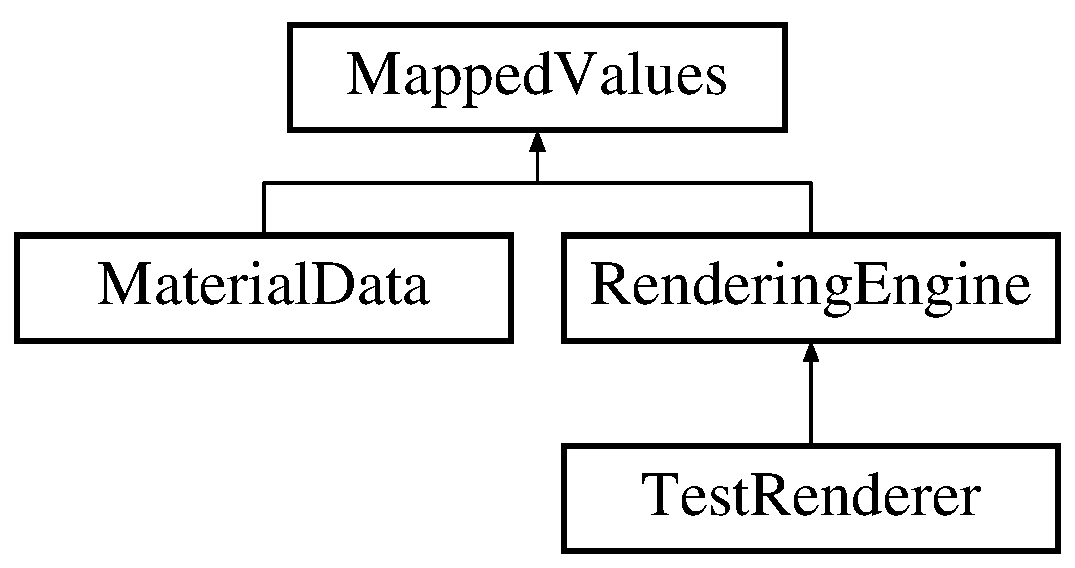
\includegraphics[height=3.000000cm]{class_mapped_values}
\end{center}
\end{figure}
\subsection*{Public Member Functions}
\begin{DoxyCompactItemize}
\item 
\hyperlink{class_mapped_values_a2f2b64544872889cf6403206f970bb7a}{Mapped\+Values} ()
\item 
void \hyperlink{class_mapped_values_aea6513980de91dc70e84a858cd470b51}{Set\+Vector3f} (const std\+::string \&name, const \hyperlink{class_vector3f}{Vector3f} \&value)
\item 
void \hyperlink{class_mapped_values_a44ae7ea73b6c2516fdd7fb0dce574300}{Set\+Float} (const std\+::string \&name, float value)
\item 
void \hyperlink{class_mapped_values_aa77284d7ea440391c052bde41996a2a3}{Set\+Texture} (const std\+::string \&name, const \hyperlink{class_texture}{Texture} \&value)
\item 
const \hyperlink{class_vector3f}{Vector3f} \& \hyperlink{class_mapped_values_a7e2399d8cb5ebd982aeffb59fe2c0854}{Get\+Vector3f} (const std\+::string \&name) const 
\item 
float \hyperlink{class_mapped_values_a8108f8905d63f905ba9a151c089c07b8}{Get\+Float} (const std\+::string \&name) const 
\item 
const \hyperlink{class_texture}{Texture} \& \hyperlink{class_mapped_values_ae63404d2d84b56f55bf6627d2f26bdc9}{Get\+Texture} (const std\+::string \&name) const 
\end{DoxyCompactItemize}


\subsection{Constructor \& Destructor Documentation}
\hypertarget{class_mapped_values_a2f2b64544872889cf6403206f970bb7a}{}\index{Mapped\+Values@{Mapped\+Values}!Mapped\+Values@{Mapped\+Values}}
\index{Mapped\+Values@{Mapped\+Values}!Mapped\+Values@{Mapped\+Values}}
\subsubsection[{Mapped\+Values()}]{\setlength{\rightskip}{0pt plus 5cm}Mapped\+Values\+::\+Mapped\+Values (
\begin{DoxyParamCaption}
{}
\end{DoxyParamCaption}
)\hspace{0.3cm}{\ttfamily [inline]}}\label{class_mapped_values_a2f2b64544872889cf6403206f970bb7a}


\subsection{Member Function Documentation}
\hypertarget{class_mapped_values_a8108f8905d63f905ba9a151c089c07b8}{}\index{Mapped\+Values@{Mapped\+Values}!Get\+Float@{Get\+Float}}
\index{Get\+Float@{Get\+Float}!Mapped\+Values@{Mapped\+Values}}
\subsubsection[{Get\+Float(const std\+::string \&name) const }]{\setlength{\rightskip}{0pt plus 5cm}float Mapped\+Values\+::\+Get\+Float (
\begin{DoxyParamCaption}
\item[{const std\+::string \&}]{name}
\end{DoxyParamCaption}
) const}\label{class_mapped_values_a8108f8905d63f905ba9a151c089c07b8}
\hypertarget{class_mapped_values_ae63404d2d84b56f55bf6627d2f26bdc9}{}\index{Mapped\+Values@{Mapped\+Values}!Get\+Texture@{Get\+Texture}}
\index{Get\+Texture@{Get\+Texture}!Mapped\+Values@{Mapped\+Values}}
\subsubsection[{Get\+Texture(const std\+::string \&name) const }]{\setlength{\rightskip}{0pt plus 5cm}const {\bf Texture} \& Mapped\+Values\+::\+Get\+Texture (
\begin{DoxyParamCaption}
\item[{const std\+::string \&}]{name}
\end{DoxyParamCaption}
) const}\label{class_mapped_values_ae63404d2d84b56f55bf6627d2f26bdc9}
\hypertarget{class_mapped_values_a7e2399d8cb5ebd982aeffb59fe2c0854}{}\index{Mapped\+Values@{Mapped\+Values}!Get\+Vector3f@{Get\+Vector3f}}
\index{Get\+Vector3f@{Get\+Vector3f}!Mapped\+Values@{Mapped\+Values}}
\subsubsection[{Get\+Vector3f(const std\+::string \&name) const }]{\setlength{\rightskip}{0pt plus 5cm}const {\bf Vector3f} \& Mapped\+Values\+::\+Get\+Vector3f (
\begin{DoxyParamCaption}
\item[{const std\+::string \&}]{name}
\end{DoxyParamCaption}
) const}\label{class_mapped_values_a7e2399d8cb5ebd982aeffb59fe2c0854}
\hypertarget{class_mapped_values_a44ae7ea73b6c2516fdd7fb0dce574300}{}\index{Mapped\+Values@{Mapped\+Values}!Set\+Float@{Set\+Float}}
\index{Set\+Float@{Set\+Float}!Mapped\+Values@{Mapped\+Values}}
\subsubsection[{Set\+Float(const std\+::string \&name, float value)}]{\setlength{\rightskip}{0pt plus 5cm}void Mapped\+Values\+::\+Set\+Float (
\begin{DoxyParamCaption}
\item[{const std\+::string \&}]{name, }
\item[{float}]{value}
\end{DoxyParamCaption}
)\hspace{0.3cm}{\ttfamily [inline]}}\label{class_mapped_values_a44ae7ea73b6c2516fdd7fb0dce574300}
\hypertarget{class_mapped_values_aa77284d7ea440391c052bde41996a2a3}{}\index{Mapped\+Values@{Mapped\+Values}!Set\+Texture@{Set\+Texture}}
\index{Set\+Texture@{Set\+Texture}!Mapped\+Values@{Mapped\+Values}}
\subsubsection[{Set\+Texture(const std\+::string \&name, const Texture \&value)}]{\setlength{\rightskip}{0pt plus 5cm}void Mapped\+Values\+::\+Set\+Texture (
\begin{DoxyParamCaption}
\item[{const std\+::string \&}]{name, }
\item[{const {\bf Texture} \&}]{value}
\end{DoxyParamCaption}
)\hspace{0.3cm}{\ttfamily [inline]}}\label{class_mapped_values_aa77284d7ea440391c052bde41996a2a3}
\hypertarget{class_mapped_values_aea6513980de91dc70e84a858cd470b51}{}\index{Mapped\+Values@{Mapped\+Values}!Set\+Vector3f@{Set\+Vector3f}}
\index{Set\+Vector3f@{Set\+Vector3f}!Mapped\+Values@{Mapped\+Values}}
\subsubsection[{Set\+Vector3f(const std\+::string \&name, const Vector3f \&value)}]{\setlength{\rightskip}{0pt plus 5cm}void Mapped\+Values\+::\+Set\+Vector3f (
\begin{DoxyParamCaption}
\item[{const std\+::string \&}]{name, }
\item[{const {\bf Vector3f} \&}]{value}
\end{DoxyParamCaption}
)\hspace{0.3cm}{\ttfamily [inline]}}\label{class_mapped_values_aea6513980de91dc70e84a858cd470b51}


The documentation for this class was generated from the following files\+:\begin{DoxyCompactItemize}
\item 
F\+:/\+Fusion3\+D\+\_\+work/src/core/\hyperlink{mapped_values_8h}{mapped\+Values.\+h}\item 
F\+:/\+Fusion3\+D\+\_\+work/src/core/\hyperlink{mapped_values_8cpp}{mapped\+Values.\+cpp}\end{DoxyCompactItemize}

\hypertarget{class_material}{}\section{Material Class Reference}
\label{class_material}\index{Material@{Material}}


{\ttfamily \#include $<$material.\+h$>$}

\subsection*{Public Member Functions}
\begin{DoxyCompactItemize}
\item 
\hyperlink{class_material_a9d10a10cc924f93d0ba35b9ada36760b}{Material} (const std\+::string \&material\+Name=\char`\"{}\char`\"{})
\item 
\hyperlink{class_material_ac9b027e9c501776e7d08589a52e9d795}{Material} (const \hyperlink{class_material}{Material} \&other)
\item 
virtual \hyperlink{class_material_a2c19452d71f54075df8f5405b03129f4}{$\sim$\+Material} ()
\item 
\hyperlink{class_material_a7ff625f38afbe0aeab9b9194848fd414}{Material} (const std\+::string \&material\+Name, const \hyperlink{class_texture}{Texture} \&diffuse, float specular\+Intensity, float specular\+Power, const \hyperlink{class_texture}{Texture} \&normal\+Map=\hyperlink{class_texture}{Texture}(\char`\"{}default\+\_\+normal.\+jpg\char`\"{}), const \hyperlink{class_texture}{Texture} \&disp\+Map=\hyperlink{class_texture}{Texture}(\char`\"{}default\+\_\+disp.\+png\char`\"{}), float disp\+Map\+Scale=0.\+0f, float disp\+Map\+Offset=0.\+0f)
\item 
void \hyperlink{class_material_a1d9130a097b656a99432d9374c887628}{Set\+Vector3f} (const std\+::string \&name, const \hyperlink{class_vector3f}{Vector3f} \&value)
\item 
void \hyperlink{class_material_a3384bed1fe3b09c204f152fb87fcd07f}{Set\+Float} (const std\+::string \&name, float value)
\item 
void \hyperlink{class_material_aa893cae3c708567d40b66af16a2b23d9}{Set\+Texture} (const std\+::string \&name, const \hyperlink{class_texture}{Texture} \&value)
\item 
const \hyperlink{class_vector3f}{Vector3f} \& \hyperlink{class_material_adbb92ca797733a8b462cda22e2483ea8}{Get\+Vector3f} (const std\+::string \&name) const 
\item 
float \hyperlink{class_material_a6460a48e7a6b759e8252d4a45e724496}{Get\+Float} (const std\+::string \&name) const 
\item 
const \hyperlink{class_texture}{Texture} \& \hyperlink{class_material_a9e100e2394f55299d8cb0556387deab3}{Get\+Texture} (const std\+::string \&name) const 
\end{DoxyCompactItemize}


\subsection{Constructor \& Destructor Documentation}
\hypertarget{class_material_a9d10a10cc924f93d0ba35b9ada36760b}{}\index{Material@{Material}!Material@{Material}}
\index{Material@{Material}!Material@{Material}}
\subsubsection[{Material(const std\+::string \&material\+Name="""")}]{\setlength{\rightskip}{0pt plus 5cm}Material\+::\+Material (
\begin{DoxyParamCaption}
\item[{const std\+::string \&}]{material\+Name = {\ttfamily \char`\"{}\char`\"{}}}
\end{DoxyParamCaption}
)}\label{class_material_a9d10a10cc924f93d0ba35b9ada36760b}
\hypertarget{class_material_ac9b027e9c501776e7d08589a52e9d795}{}\index{Material@{Material}!Material@{Material}}
\index{Material@{Material}!Material@{Material}}
\subsubsection[{Material(const Material \&other)}]{\setlength{\rightskip}{0pt plus 5cm}Material\+::\+Material (
\begin{DoxyParamCaption}
\item[{const {\bf Material} \&}]{other}
\end{DoxyParamCaption}
)}\label{class_material_ac9b027e9c501776e7d08589a52e9d795}
\hypertarget{class_material_a2c19452d71f54075df8f5405b03129f4}{}\index{Material@{Material}!````~Material@{$\sim$\+Material}}
\index{````~Material@{$\sim$\+Material}!Material@{Material}}
\subsubsection[{$\sim$\+Material()}]{\setlength{\rightskip}{0pt plus 5cm}Material\+::$\sim$\+Material (
\begin{DoxyParamCaption}
{}
\end{DoxyParamCaption}
)\hspace{0.3cm}{\ttfamily [virtual]}}\label{class_material_a2c19452d71f54075df8f5405b03129f4}
\hypertarget{class_material_a7ff625f38afbe0aeab9b9194848fd414}{}\index{Material@{Material}!Material@{Material}}
\index{Material@{Material}!Material@{Material}}
\subsubsection[{Material(const std\+::string \&material\+Name, const Texture \&diffuse, float specular\+Intensity, float specular\+Power, const Texture \&normal\+Map=\+Texture(""default\+\_\+normal.\+jpg""), const Texture \&disp\+Map=\+Texture(""default\+\_\+disp.\+png""), float disp\+Map\+Scale=0.\+0f, float disp\+Map\+Offset=0.\+0f)}]{\setlength{\rightskip}{0pt plus 5cm}Material\+::\+Material (
\begin{DoxyParamCaption}
\item[{const std\+::string \&}]{material\+Name, }
\item[{const {\bf Texture} \&}]{diffuse, }
\item[{float}]{specular\+Intensity, }
\item[{float}]{specular\+Power, }
\item[{const {\bf Texture} \&}]{normal\+Map = {\ttfamily {\bf Texture}(\char`\"{}default\+\_\+normal.jpg\char`\"{})}, }
\item[{const {\bf Texture} \&}]{disp\+Map = {\ttfamily {\bf Texture}(\char`\"{}default\+\_\+disp.png\char`\"{})}, }
\item[{float}]{disp\+Map\+Scale = {\ttfamily 0.0f}, }
\item[{float}]{disp\+Map\+Offset = {\ttfamily 0.0f}}
\end{DoxyParamCaption}
)}\label{class_material_a7ff625f38afbe0aeab9b9194848fd414}


\subsection{Member Function Documentation}
\hypertarget{class_material_a6460a48e7a6b759e8252d4a45e724496}{}\index{Material@{Material}!Get\+Float@{Get\+Float}}
\index{Get\+Float@{Get\+Float}!Material@{Material}}
\subsubsection[{Get\+Float(const std\+::string \&name) const }]{\setlength{\rightskip}{0pt plus 5cm}float Material\+::\+Get\+Float (
\begin{DoxyParamCaption}
\item[{const std\+::string \&}]{name}
\end{DoxyParamCaption}
) const\hspace{0.3cm}{\ttfamily [inline]}}\label{class_material_a6460a48e7a6b759e8252d4a45e724496}
\hypertarget{class_material_a9e100e2394f55299d8cb0556387deab3}{}\index{Material@{Material}!Get\+Texture@{Get\+Texture}}
\index{Get\+Texture@{Get\+Texture}!Material@{Material}}
\subsubsection[{Get\+Texture(const std\+::string \&name) const }]{\setlength{\rightskip}{0pt plus 5cm}const {\bf Texture}\& Material\+::\+Get\+Texture (
\begin{DoxyParamCaption}
\item[{const std\+::string \&}]{name}
\end{DoxyParamCaption}
) const\hspace{0.3cm}{\ttfamily [inline]}}\label{class_material_a9e100e2394f55299d8cb0556387deab3}
\hypertarget{class_material_adbb92ca797733a8b462cda22e2483ea8}{}\index{Material@{Material}!Get\+Vector3f@{Get\+Vector3f}}
\index{Get\+Vector3f@{Get\+Vector3f}!Material@{Material}}
\subsubsection[{Get\+Vector3f(const std\+::string \&name) const }]{\setlength{\rightskip}{0pt plus 5cm}const {\bf Vector3f}\& Material\+::\+Get\+Vector3f (
\begin{DoxyParamCaption}
\item[{const std\+::string \&}]{name}
\end{DoxyParamCaption}
) const\hspace{0.3cm}{\ttfamily [inline]}}\label{class_material_adbb92ca797733a8b462cda22e2483ea8}
\hypertarget{class_material_a3384bed1fe3b09c204f152fb87fcd07f}{}\index{Material@{Material}!Set\+Float@{Set\+Float}}
\index{Set\+Float@{Set\+Float}!Material@{Material}}
\subsubsection[{Set\+Float(const std\+::string \&name, float value)}]{\setlength{\rightskip}{0pt plus 5cm}void Material\+::\+Set\+Float (
\begin{DoxyParamCaption}
\item[{const std\+::string \&}]{name, }
\item[{float}]{value}
\end{DoxyParamCaption}
)\hspace{0.3cm}{\ttfamily [inline]}}\label{class_material_a3384bed1fe3b09c204f152fb87fcd07f}
\hypertarget{class_material_aa893cae3c708567d40b66af16a2b23d9}{}\index{Material@{Material}!Set\+Texture@{Set\+Texture}}
\index{Set\+Texture@{Set\+Texture}!Material@{Material}}
\subsubsection[{Set\+Texture(const std\+::string \&name, const Texture \&value)}]{\setlength{\rightskip}{0pt plus 5cm}void Material\+::\+Set\+Texture (
\begin{DoxyParamCaption}
\item[{const std\+::string \&}]{name, }
\item[{const {\bf Texture} \&}]{value}
\end{DoxyParamCaption}
)\hspace{0.3cm}{\ttfamily [inline]}}\label{class_material_aa893cae3c708567d40b66af16a2b23d9}
\hypertarget{class_material_a1d9130a097b656a99432d9374c887628}{}\index{Material@{Material}!Set\+Vector3f@{Set\+Vector3f}}
\index{Set\+Vector3f@{Set\+Vector3f}!Material@{Material}}
\subsubsection[{Set\+Vector3f(const std\+::string \&name, const Vector3f \&value)}]{\setlength{\rightskip}{0pt plus 5cm}void Material\+::\+Set\+Vector3f (
\begin{DoxyParamCaption}
\item[{const std\+::string \&}]{name, }
\item[{const {\bf Vector3f} \&}]{value}
\end{DoxyParamCaption}
)\hspace{0.3cm}{\ttfamily [inline]}}\label{class_material_a1d9130a097b656a99432d9374c887628}


The documentation for this class was generated from the following files\+:\begin{DoxyCompactItemize}
\item 
F\+:/\+Fusion3\+D\+\_\+work/src/rendering/\hyperlink{material_8h}{material.\+h}\item 
F\+:/\+Fusion3\+D\+\_\+work/src/rendering/\hyperlink{material_8cpp}{material.\+cpp}\end{DoxyCompactItemize}

\hypertarget{class_material_data}{}\section{Material\+Data Class Reference}
\label{class_material_data}\index{Material\+Data@{Material\+Data}}


{\ttfamily \#include $<$material.\+h$>$}

Inheritance diagram for Material\+Data\+:\begin{figure}[H]
\begin{center}
\leavevmode
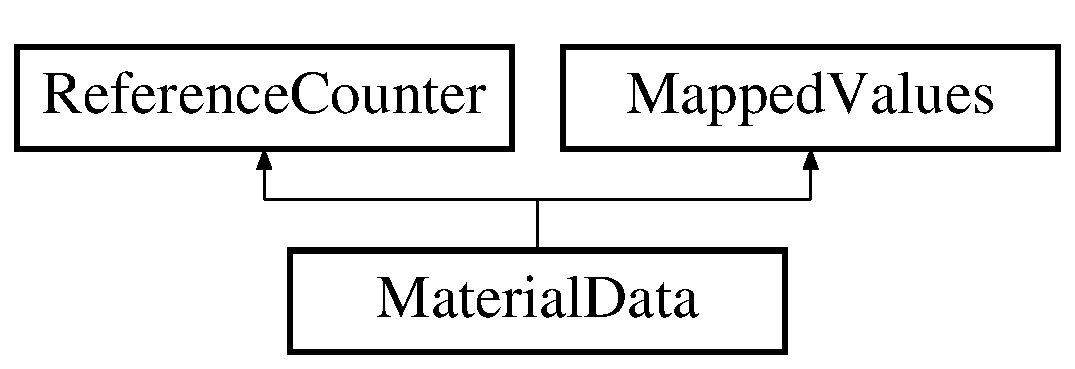
\includegraphics[height=2.000000cm]{class_material_data}
\end{center}
\end{figure}
\subsection*{Additional Inherited Members}


The documentation for this class was generated from the following file\+:\begin{DoxyCompactItemize}
\item 
F\+:/\+Fusion3\+D\+\_\+work/src/rendering/\hyperlink{material_8h}{material.\+h}\end{DoxyCompactItemize}

\hypertarget{class_matrix}{}\section{Matrix$<$ T, D $>$ Class Template Reference}
\label{class_matrix}\index{Matrix$<$ T, D $>$@{Matrix$<$ T, D $>$}}


{\ttfamily \#include $<$math3d.\+h$>$}

\subsection*{Public Member Functions}
\begin{DoxyCompactItemize}
\item 
\hyperlink{class_matrix}{Matrix}$<$ T, D $>$ \hyperlink{class_matrix_aa6653ba9d81668d11bfafae3df9d7e36}{Init\+Identity} ()
\item 
\hyperlink{class_matrix}{Matrix}$<$ T, D $>$ \hyperlink{class_matrix_a669ac3058ca94ee6bcb0bb6d65693942}{Init\+Scale} (const \hyperlink{class_vector}{Vector}$<$ T, D-\/1 $>$ \&r)
\item 
\hyperlink{class_matrix}{Matrix}$<$ T, D $>$ \hyperlink{class_matrix_a085e7210b168aaa55c2c9c5932d33fd7}{Init\+Translation} (const \hyperlink{class_vector}{Vector}$<$ T, D-\/1 $>$ \&r)
\item 
\hyperlink{class_matrix}{Matrix}$<$ T, D $>$ \hyperlink{class_matrix_ada41ba03c5fd295ce9fccfaee4fcc8c9}{Transpose} () const 
\item 
\hyperlink{class_matrix}{Matrix}$<$ T, D $>$ \hyperlink{class_matrix_a5f645b7f8f35938348ededc07e2f689c}{Inverse} () const 
\item 
\hyperlink{class_matrix}{Matrix}$<$ T, D $>$ \hyperlink{class_matrix_a4e4a905d09213282c802a90d44d693c6}{operator$\ast$} (const \hyperlink{class_matrix}{Matrix}$<$ T, D $>$ \&r) const 
\item 
\hyperlink{class_vector}{Vector}$<$ T, D $>$ \hyperlink{class_matrix_af57977803e2ec19bfbc9ab56b9afaed1}{Transform} (const \hyperlink{class_vector}{Vector}$<$ T, D $>$ \&r) const 
\item 
\hyperlink{class_vector}{Vector}$<$ T, D-\/1 $>$ \hyperlink{class_matrix_af9c8c3f95c7f4d5af195695c552d88da}{Transform} (const \hyperlink{class_vector}{Vector}$<$ T, D-\/1 $>$ \&r) const 
\item 
void \hyperlink{class_matrix_a24005a942d94e7dae6a6c6d076d9b6fa}{Set} (unsigned int x, unsigned int y, T val)
\item 
const T $\ast$ \hyperlink{class_matrix_af32d2322ab44e083492cfd91b80d5418}{operator\mbox{[}$\,$\mbox{]}} (int index) const 
\item 
T $\ast$ \hyperlink{class_matrix_ae5706ecdcc918c8b0c4e94d3360d629e}{operator\mbox{[}$\,$\mbox{]}} (int index)
\end{DoxyCompactItemize}


\subsection{Member Function Documentation}
\hypertarget{class_matrix_aa6653ba9d81668d11bfafae3df9d7e36}{}\index{Matrix@{Matrix}!Init\+Identity@{Init\+Identity}}
\index{Init\+Identity@{Init\+Identity}!Matrix@{Matrix}}
\subsubsection[{Init\+Identity()}]{\setlength{\rightskip}{0pt plus 5cm}template$<$typename T, unsigned int D$>$ {\bf Matrix}$<$T, D$>$ {\bf Matrix}$<$ T, D $>$\+::Init\+Identity (
\begin{DoxyParamCaption}
{}
\end{DoxyParamCaption}
)\hspace{0.3cm}{\ttfamily [inline]}}\label{class_matrix_aa6653ba9d81668d11bfafae3df9d7e36}
\hypertarget{class_matrix_a669ac3058ca94ee6bcb0bb6d65693942}{}\index{Matrix@{Matrix}!Init\+Scale@{Init\+Scale}}
\index{Init\+Scale@{Init\+Scale}!Matrix@{Matrix}}
\subsubsection[{Init\+Scale(const Vector$<$ T, D-\/1 $>$ \&r)}]{\setlength{\rightskip}{0pt plus 5cm}template$<$typename T, unsigned int D$>$ {\bf Matrix}$<$T, D$>$ {\bf Matrix}$<$ T, D $>$\+::Init\+Scale (
\begin{DoxyParamCaption}
\item[{const {\bf Vector}$<$ T, D-\/1 $>$ \&}]{r}
\end{DoxyParamCaption}
)\hspace{0.3cm}{\ttfamily [inline]}}\label{class_matrix_a669ac3058ca94ee6bcb0bb6d65693942}
\hypertarget{class_matrix_a085e7210b168aaa55c2c9c5932d33fd7}{}\index{Matrix@{Matrix}!Init\+Translation@{Init\+Translation}}
\index{Init\+Translation@{Init\+Translation}!Matrix@{Matrix}}
\subsubsection[{Init\+Translation(const Vector$<$ T, D-\/1 $>$ \&r)}]{\setlength{\rightskip}{0pt plus 5cm}template$<$typename T, unsigned int D$>$ {\bf Matrix}$<$T, D$>$ {\bf Matrix}$<$ T, D $>$\+::Init\+Translation (
\begin{DoxyParamCaption}
\item[{const {\bf Vector}$<$ T, D-\/1 $>$ \&}]{r}
\end{DoxyParamCaption}
)\hspace{0.3cm}{\ttfamily [inline]}}\label{class_matrix_a085e7210b168aaa55c2c9c5932d33fd7}
\hypertarget{class_matrix_a5f645b7f8f35938348ededc07e2f689c}{}\index{Matrix@{Matrix}!Inverse@{Inverse}}
\index{Inverse@{Inverse}!Matrix@{Matrix}}
\subsubsection[{Inverse() const }]{\setlength{\rightskip}{0pt plus 5cm}template$<$typename T, unsigned int D$>$ {\bf Matrix}$<$T, D$>$ {\bf Matrix}$<$ T, D $>$\+::Inverse (
\begin{DoxyParamCaption}
{}
\end{DoxyParamCaption}
) const\hspace{0.3cm}{\ttfamily [inline]}}\label{class_matrix_a5f645b7f8f35938348ededc07e2f689c}
\hypertarget{class_matrix_a4e4a905d09213282c802a90d44d693c6}{}\index{Matrix@{Matrix}!operator$\ast$@{operator$\ast$}}
\index{operator$\ast$@{operator$\ast$}!Matrix@{Matrix}}
\subsubsection[{operator$\ast$(const Matrix$<$ T, D $>$ \&r) const }]{\setlength{\rightskip}{0pt plus 5cm}template$<$typename T, unsigned int D$>$ {\bf Matrix}$<$T,D$>$ {\bf Matrix}$<$ T, D $>$\+::operator$\ast$ (
\begin{DoxyParamCaption}
\item[{const {\bf Matrix}$<$ T, D $>$ \&}]{r}
\end{DoxyParamCaption}
) const\hspace{0.3cm}{\ttfamily [inline]}}\label{class_matrix_a4e4a905d09213282c802a90d44d693c6}
\hypertarget{class_matrix_af32d2322ab44e083492cfd91b80d5418}{}\index{Matrix@{Matrix}!operator\mbox{[}$\,$\mbox{]}@{operator[]}}
\index{operator\mbox{[}$\,$\mbox{]}@{operator[]}!Matrix@{Matrix}}
\subsubsection[{operator[](int index) const }]{\setlength{\rightskip}{0pt plus 5cm}template$<$typename T, unsigned int D$>$ const T$\ast$ {\bf Matrix}$<$ T, D $>$\+::operator\mbox{[}$\,$\mbox{]} (
\begin{DoxyParamCaption}
\item[{int}]{index}
\end{DoxyParamCaption}
) const\hspace{0.3cm}{\ttfamily [inline]}}\label{class_matrix_af32d2322ab44e083492cfd91b80d5418}
\hypertarget{class_matrix_ae5706ecdcc918c8b0c4e94d3360d629e}{}\index{Matrix@{Matrix}!operator\mbox{[}$\,$\mbox{]}@{operator[]}}
\index{operator\mbox{[}$\,$\mbox{]}@{operator[]}!Matrix@{Matrix}}
\subsubsection[{operator[](int index)}]{\setlength{\rightskip}{0pt plus 5cm}template$<$typename T, unsigned int D$>$ T$\ast$ {\bf Matrix}$<$ T, D $>$\+::operator\mbox{[}$\,$\mbox{]} (
\begin{DoxyParamCaption}
\item[{int}]{index}
\end{DoxyParamCaption}
)\hspace{0.3cm}{\ttfamily [inline]}}\label{class_matrix_ae5706ecdcc918c8b0c4e94d3360d629e}
\hypertarget{class_matrix_a24005a942d94e7dae6a6c6d076d9b6fa}{}\index{Matrix@{Matrix}!Set@{Set}}
\index{Set@{Set}!Matrix@{Matrix}}
\subsubsection[{Set(unsigned int x, unsigned int y, T val)}]{\setlength{\rightskip}{0pt plus 5cm}template$<$typename T, unsigned int D$>$ void {\bf Matrix}$<$ T, D $>$\+::Set (
\begin{DoxyParamCaption}
\item[{unsigned int}]{x, }
\item[{unsigned int}]{y, }
\item[{T}]{val}
\end{DoxyParamCaption}
)\hspace{0.3cm}{\ttfamily [inline]}}\label{class_matrix_a24005a942d94e7dae6a6c6d076d9b6fa}
\hypertarget{class_matrix_af57977803e2ec19bfbc9ab56b9afaed1}{}\index{Matrix@{Matrix}!Transform@{Transform}}
\index{Transform@{Transform}!Matrix@{Matrix}}
\subsubsection[{Transform(const Vector$<$ T, D $>$ \&r) const }]{\setlength{\rightskip}{0pt plus 5cm}template$<$typename T, unsigned int D$>$ {\bf Vector}$<$T,D$>$ {\bf Matrix}$<$ T, D $>$\+::{\bf Transform} (
\begin{DoxyParamCaption}
\item[{const {\bf Vector}$<$ T, D $>$ \&}]{r}
\end{DoxyParamCaption}
) const\hspace{0.3cm}{\ttfamily [inline]}}\label{class_matrix_af57977803e2ec19bfbc9ab56b9afaed1}
\hypertarget{class_matrix_af9c8c3f95c7f4d5af195695c552d88da}{}\index{Matrix@{Matrix}!Transform@{Transform}}
\index{Transform@{Transform}!Matrix@{Matrix}}
\subsubsection[{Transform(const Vector$<$ T, D-\/1 $>$ \&r) const }]{\setlength{\rightskip}{0pt plus 5cm}template$<$typename T, unsigned int D$>$ {\bf Vector}$<$T,D-\/1$>$ {\bf Matrix}$<$ T, D $>$\+::{\bf Transform} (
\begin{DoxyParamCaption}
\item[{const {\bf Vector}$<$ T, D-\/1 $>$ \&}]{r}
\end{DoxyParamCaption}
) const\hspace{0.3cm}{\ttfamily [inline]}}\label{class_matrix_af9c8c3f95c7f4d5af195695c552d88da}
\hypertarget{class_matrix_ada41ba03c5fd295ce9fccfaee4fcc8c9}{}\index{Matrix@{Matrix}!Transpose@{Transpose}}
\index{Transpose@{Transpose}!Matrix@{Matrix}}
\subsubsection[{Transpose() const }]{\setlength{\rightskip}{0pt plus 5cm}template$<$typename T, unsigned int D$>$ {\bf Matrix}$<$T, D$>$ {\bf Matrix}$<$ T, D $>$\+::Transpose (
\begin{DoxyParamCaption}
{}
\end{DoxyParamCaption}
) const\hspace{0.3cm}{\ttfamily [inline]}}\label{class_matrix_ada41ba03c5fd295ce9fccfaee4fcc8c9}


The documentation for this class was generated from the following file\+:\begin{DoxyCompactItemize}
\item 
F\+:/\+Fusion3\+D\+\_\+work/src/core/\hyperlink{math3d_8h}{math3d.\+h}\end{DoxyCompactItemize}

\hypertarget{class_matrix3}{}\section{Matrix3$<$ T $>$ Class Template Reference}
\label{class_matrix3}\index{Matrix3$<$ T $>$@{Matrix3$<$ T $>$}}


{\ttfamily \#include $<$math3d.\+h$>$}

Inheritance diagram for Matrix3$<$ T $>$\+:\begin{figure}[H]
\begin{center}
\leavevmode
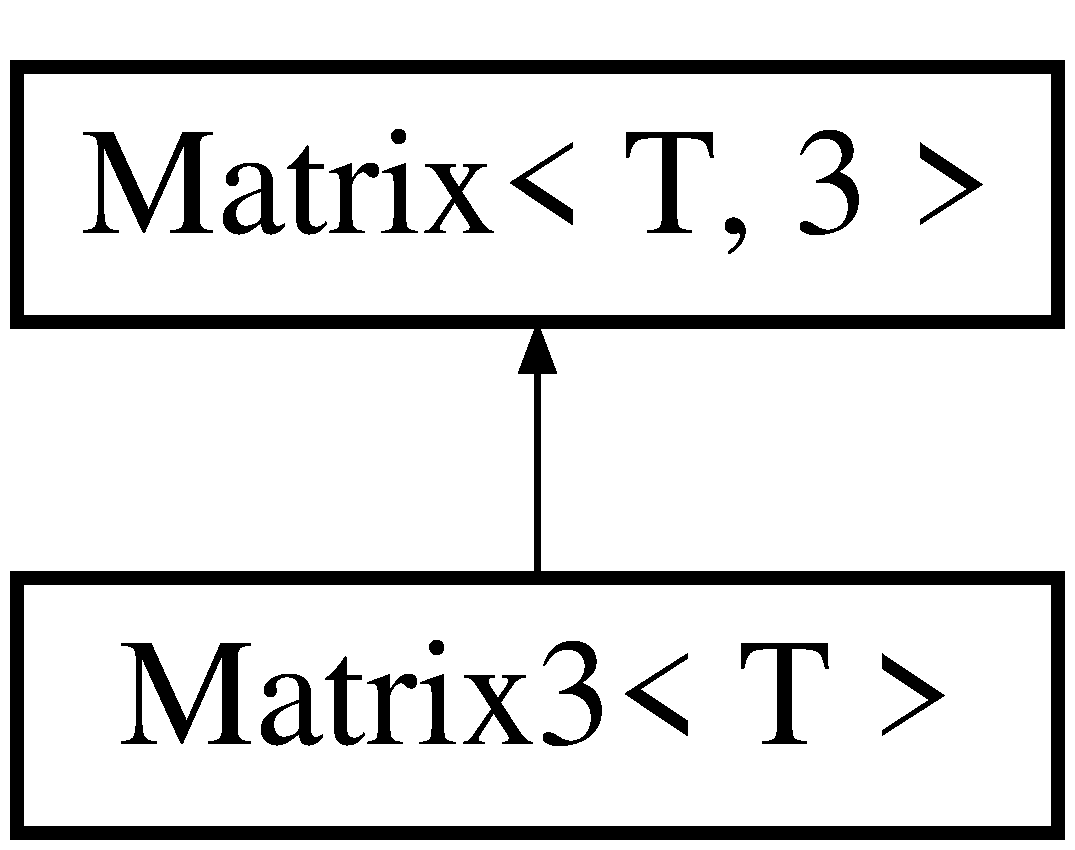
\includegraphics[height=2.000000cm]{class_matrix3}
\end{center}
\end{figure}
\subsection*{Public Member Functions}
\begin{DoxyCompactItemize}
\item 
\hyperlink{class_matrix3_afbc8b655540e4b5b04d8439b606303b0}{Matrix3} ()
\item 
{\footnotesize template$<$unsigned int D$>$ }\\\hyperlink{class_matrix3_ac47eddcab53aef5812f04cb5ee2f4f0a}{Matrix3} (const \hyperlink{class_matrix}{Matrix}$<$ T, D $>$ \&r)
\end{DoxyCompactItemize}


\subsection{Constructor \& Destructor Documentation}
\hypertarget{class_matrix3_afbc8b655540e4b5b04d8439b606303b0}{}\index{Matrix3@{Matrix3}!Matrix3@{Matrix3}}
\index{Matrix3@{Matrix3}!Matrix3@{Matrix3}}
\subsubsection[{Matrix3()}]{\setlength{\rightskip}{0pt plus 5cm}template$<$typename T $>$ {\bf Matrix3}$<$ T $>$\+::{\bf Matrix3} (
\begin{DoxyParamCaption}
{}
\end{DoxyParamCaption}
)\hspace{0.3cm}{\ttfamily [inline]}}\label{class_matrix3_afbc8b655540e4b5b04d8439b606303b0}
\hypertarget{class_matrix3_ac47eddcab53aef5812f04cb5ee2f4f0a}{}\index{Matrix3@{Matrix3}!Matrix3@{Matrix3}}
\index{Matrix3@{Matrix3}!Matrix3@{Matrix3}}
\subsubsection[{Matrix3(const Matrix$<$ T, D $>$ \&r)}]{\setlength{\rightskip}{0pt plus 5cm}template$<$typename T $>$ template$<$unsigned int D$>$ {\bf Matrix3}$<$ T $>$\+::{\bf Matrix3} (
\begin{DoxyParamCaption}
\item[{const {\bf Matrix}$<$ T, D $>$ \&}]{r}
\end{DoxyParamCaption}
)\hspace{0.3cm}{\ttfamily [inline]}}\label{class_matrix3_ac47eddcab53aef5812f04cb5ee2f4f0a}


The documentation for this class was generated from the following file\+:\begin{DoxyCompactItemize}
\item 
F\+:/\+Fusion3\+D\+\_\+work/src/core/\hyperlink{math3d_8h}{math3d.\+h}\end{DoxyCompactItemize}

\hypertarget{class_matrix4}{}\section{Matrix4$<$ T $>$ Class Template Reference}
\label{class_matrix4}\index{Matrix4$<$ T $>$@{Matrix4$<$ T $>$}}


{\ttfamily \#include $<$math3d.\+h$>$}

Inheritance diagram for Matrix4$<$ T $>$\+:\begin{figure}[H]
\begin{center}
\leavevmode
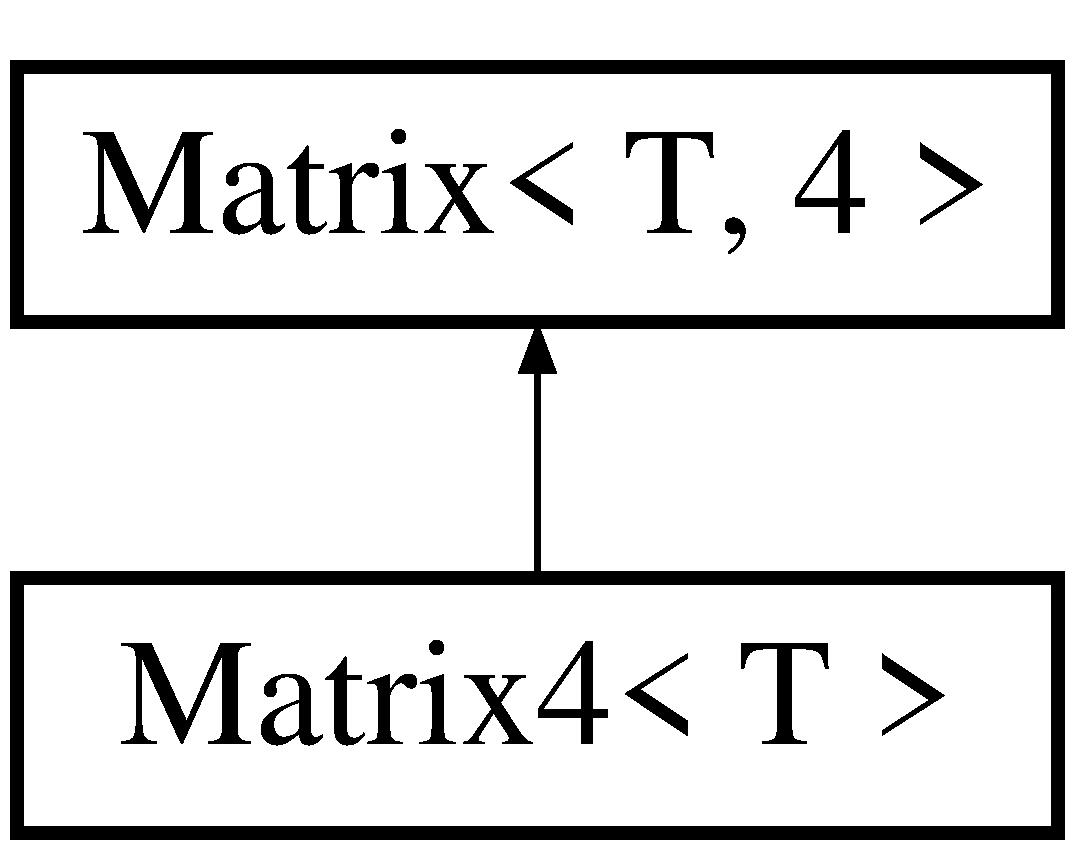
\includegraphics[height=2.000000cm]{class_matrix4}
\end{center}
\end{figure}
\subsection*{Public Member Functions}
\begin{DoxyCompactItemize}
\item 
\hyperlink{class_matrix4_ab24760b5fdf4cac34df976d6820394c2}{Matrix4} ()
\item 
{\footnotesize template$<$unsigned int D$>$ }\\\hyperlink{class_matrix4_a46d918dcaacec9b797070451aa96d284}{Matrix4} (const \hyperlink{class_matrix}{Matrix}$<$ T, D $>$ \&r)
\item 
\hyperlink{class_matrix4}{Matrix4}$<$ T $>$ \hyperlink{class_matrix4_a1401d365cfc879742cc07d7a29e4a4a8}{Init\+Rotation\+Euler} (T rotate\+X, T rotate\+Y, T rotate\+Z)
\item 
\hyperlink{class_matrix4}{Matrix4}$<$ T $>$ \hyperlink{class_matrix4_aea8381025c2551b6315197908fe11542}{Init\+Rotation\+From\+Vectors} (const \hyperlink{class_vector3}{Vector3}$<$ T $>$ \&n, const \hyperlink{class_vector3}{Vector3}$<$ T $>$ \&v, const \hyperlink{class_vector3}{Vector3}$<$ T $>$ \&u)
\item 
\hyperlink{class_matrix4}{Matrix4}$<$ T $>$ \hyperlink{class_matrix4_a4f34bc6810473b714a995fa462902e61}{Init\+Rotation\+From\+Direction} (const \hyperlink{class_vector3}{Vector3}$<$ T $>$ \&forward, const \hyperlink{class_vector3}{Vector3}$<$ T $>$ \&up)
\item 
\hyperlink{class_matrix4}{Matrix4}$<$ T $>$ \hyperlink{class_matrix4_a827b624535c1d251d91a2f2b187f7045}{Init\+Perspective} (T fov, T aspect\+Ratio, T z\+Near, T z\+Far)
\item 
\hyperlink{class_matrix4}{Matrix4}$<$ T $>$ \hyperlink{class_matrix4_a37a521c8175747731ff2003b2924375d}{Init\+Orthographic} (T left, T right, T bottom, T top, T near, T far)
\end{DoxyCompactItemize}


\subsection{Constructor \& Destructor Documentation}
\hypertarget{class_matrix4_ab24760b5fdf4cac34df976d6820394c2}{}\index{Matrix4@{Matrix4}!Matrix4@{Matrix4}}
\index{Matrix4@{Matrix4}!Matrix4@{Matrix4}}
\subsubsection[{Matrix4()}]{\setlength{\rightskip}{0pt plus 5cm}template$<$typename T$>$ {\bf Matrix4}$<$ T $>$\+::{\bf Matrix4} (
\begin{DoxyParamCaption}
{}
\end{DoxyParamCaption}
)\hspace{0.3cm}{\ttfamily [inline]}}\label{class_matrix4_ab24760b5fdf4cac34df976d6820394c2}
\hypertarget{class_matrix4_a46d918dcaacec9b797070451aa96d284}{}\index{Matrix4@{Matrix4}!Matrix4@{Matrix4}}
\index{Matrix4@{Matrix4}!Matrix4@{Matrix4}}
\subsubsection[{Matrix4(const Matrix$<$ T, D $>$ \&r)}]{\setlength{\rightskip}{0pt plus 5cm}template$<$typename T$>$ template$<$unsigned int D$>$ {\bf Matrix4}$<$ T $>$\+::{\bf Matrix4} (
\begin{DoxyParamCaption}
\item[{const {\bf Matrix}$<$ T, D $>$ \&}]{r}
\end{DoxyParamCaption}
)\hspace{0.3cm}{\ttfamily [inline]}}\label{class_matrix4_a46d918dcaacec9b797070451aa96d284}


\subsection{Member Function Documentation}
\hypertarget{class_matrix4_a37a521c8175747731ff2003b2924375d}{}\index{Matrix4@{Matrix4}!Init\+Orthographic@{Init\+Orthographic}}
\index{Init\+Orthographic@{Init\+Orthographic}!Matrix4@{Matrix4}}
\subsubsection[{Init\+Orthographic(\+T left, T right, T bottom, T top, T near, T far)}]{\setlength{\rightskip}{0pt plus 5cm}template$<$typename T$>$ {\bf Matrix4}$<$T$>$ {\bf Matrix4}$<$ T $>$\+::Init\+Orthographic (
\begin{DoxyParamCaption}
\item[{T}]{left, }
\item[{T}]{right, }
\item[{T}]{bottom, }
\item[{T}]{top, }
\item[{T}]{near, }
\item[{T}]{far}
\end{DoxyParamCaption}
)\hspace{0.3cm}{\ttfamily [inline]}}\label{class_matrix4_a37a521c8175747731ff2003b2924375d}
\hypertarget{class_matrix4_a827b624535c1d251d91a2f2b187f7045}{}\index{Matrix4@{Matrix4}!Init\+Perspective@{Init\+Perspective}}
\index{Init\+Perspective@{Init\+Perspective}!Matrix4@{Matrix4}}
\subsubsection[{Init\+Perspective(\+T fov, T aspect\+Ratio, T z\+Near, T z\+Far)}]{\setlength{\rightskip}{0pt plus 5cm}template$<$typename T$>$ {\bf Matrix4}$<$T$>$ {\bf Matrix4}$<$ T $>$\+::Init\+Perspective (
\begin{DoxyParamCaption}
\item[{T}]{fov, }
\item[{T}]{aspect\+Ratio, }
\item[{T}]{z\+Near, }
\item[{T}]{z\+Far}
\end{DoxyParamCaption}
)\hspace{0.3cm}{\ttfamily [inline]}}\label{class_matrix4_a827b624535c1d251d91a2f2b187f7045}
\hypertarget{class_matrix4_a1401d365cfc879742cc07d7a29e4a4a8}{}\index{Matrix4@{Matrix4}!Init\+Rotation\+Euler@{Init\+Rotation\+Euler}}
\index{Init\+Rotation\+Euler@{Init\+Rotation\+Euler}!Matrix4@{Matrix4}}
\subsubsection[{Init\+Rotation\+Euler(\+T rotate\+X, T rotate\+Y, T rotate\+Z)}]{\setlength{\rightskip}{0pt plus 5cm}template$<$typename T$>$ {\bf Matrix4}$<$T$>$ {\bf Matrix4}$<$ T $>$\+::Init\+Rotation\+Euler (
\begin{DoxyParamCaption}
\item[{T}]{rotate\+X, }
\item[{T}]{rotate\+Y, }
\item[{T}]{rotate\+Z}
\end{DoxyParamCaption}
)\hspace{0.3cm}{\ttfamily [inline]}}\label{class_matrix4_a1401d365cfc879742cc07d7a29e4a4a8}
\hypertarget{class_matrix4_a4f34bc6810473b714a995fa462902e61}{}\index{Matrix4@{Matrix4}!Init\+Rotation\+From\+Direction@{Init\+Rotation\+From\+Direction}}
\index{Init\+Rotation\+From\+Direction@{Init\+Rotation\+From\+Direction}!Matrix4@{Matrix4}}
\subsubsection[{Init\+Rotation\+From\+Direction(const Vector3$<$ T $>$ \&forward, const Vector3$<$ T $>$ \&up)}]{\setlength{\rightskip}{0pt plus 5cm}template$<$typename T$>$ {\bf Matrix4}$<$T$>$ {\bf Matrix4}$<$ T $>$\+::Init\+Rotation\+From\+Direction (
\begin{DoxyParamCaption}
\item[{const {\bf Vector3}$<$ T $>$ \&}]{forward, }
\item[{const {\bf Vector3}$<$ T $>$ \&}]{up}
\end{DoxyParamCaption}
)\hspace{0.3cm}{\ttfamily [inline]}}\label{class_matrix4_a4f34bc6810473b714a995fa462902e61}
\hypertarget{class_matrix4_aea8381025c2551b6315197908fe11542}{}\index{Matrix4@{Matrix4}!Init\+Rotation\+From\+Vectors@{Init\+Rotation\+From\+Vectors}}
\index{Init\+Rotation\+From\+Vectors@{Init\+Rotation\+From\+Vectors}!Matrix4@{Matrix4}}
\subsubsection[{Init\+Rotation\+From\+Vectors(const Vector3$<$ T $>$ \&n, const Vector3$<$ T $>$ \&v, const Vector3$<$ T $>$ \&u)}]{\setlength{\rightskip}{0pt plus 5cm}template$<$typename T$>$ {\bf Matrix4}$<$T$>$ {\bf Matrix4}$<$ T $>$\+::Init\+Rotation\+From\+Vectors (
\begin{DoxyParamCaption}
\item[{const {\bf Vector3}$<$ T $>$ \&}]{n, }
\item[{const {\bf Vector3}$<$ T $>$ \&}]{v, }
\item[{const {\bf Vector3}$<$ T $>$ \&}]{u}
\end{DoxyParamCaption}
)\hspace{0.3cm}{\ttfamily [inline]}}\label{class_matrix4_aea8381025c2551b6315197908fe11542}


The documentation for this class was generated from the following file\+:\begin{DoxyCompactItemize}
\item 
F\+:/\+Fusion3\+D\+\_\+work/src/core/\hyperlink{math3d_8h}{math3d.\+h}\end{DoxyCompactItemize}

\hypertarget{class_mesh}{}\section{Mesh Class Reference}
\label{class_mesh}\index{Mesh@{Mesh}}


{\ttfamily \#include $<$mesh.\+h$>$}

\subsection*{Public Member Functions}
\begin{DoxyCompactItemize}
\item 
\hyperlink{class_mesh_a167934b0e617950bf4df22ea01b8704b}{Mesh} (const std\+::string \&file\+Name=\char`\"{}cube.\+obj\char`\"{})
\item 
\hyperlink{class_mesh_af2822b45c3cb647736cda3db9886dce2}{Mesh} (const std\+::string \&file\+Name, \hyperlink{class_mesh_data}{Mesh\+Data} $\ast$data)
\item 
\hyperlink{class_mesh_a077a578c62a22809ac88e47412a0c8cc}{Mesh} (const std\+::string \&mesh\+Name, const \hyperlink{class_indexed_model}{Indexed\+Model} \&model)
\item 
\hyperlink{class_mesh_ad0260249329b621d4d91c66293baef8d}{Mesh} (const \hyperlink{class_mesh}{Mesh} \&mesh)
\item 
virtual \hyperlink{class_mesh_a5efe4da1a4c0971cfb037bd70304c303}{$\sim$\+Mesh} ()
\item 
void \hyperlink{class_mesh_a295f283d6a6a2ca8e8e46e2fc2fbe727}{Draw} () const 
\item 
\hyperlink{class_mesh_data}{Mesh\+Data} $\ast$ \hyperlink{class_mesh_a957ca65ff9f05a82e8c50f3ac72b8618}{Get\+Mesh\+Data} () const 
\end{DoxyCompactItemize}
\subsection*{Static Public Member Functions}
\begin{DoxyCompactItemize}
\item 
static std\+::vector$<$ \hyperlink{class_mesh_data}{Mesh\+Data} $\ast$ $>$ \hyperlink{class_mesh_a7d62297804518c08fe8429dea702d4af}{Import\+Mesh\+Data} (const std\+::string \&file\+Name, int mode=-\/1)
\item 
static bt\+Triangle\+Mesh $\ast$ \hyperlink{class_mesh_a9834cb2e2924821f36b0c3e2a4c326e7}{Import\+Col\+Data} (const std\+::string \&file\+Name)
\item 
static std\+::vector$<$ \hyperlink{class_material}{Material} $\ast$ $>$ \hyperlink{class_mesh_ad1a6c1004ac4e073852989a3d68538d1}{Import\+Mesh\+Material} (const std\+::string \&file\+Name)
\item 
static std\+::vector$<$ \hyperlink{class_mesh}{Mesh} $\ast$ $>$ \hyperlink{class_mesh_af11b125a96697494a80c864e3d7c1864}{Import\+Mesh} (const std\+::string \&file\+Name)
\item 
static bt\+Triangle\+Mesh $\ast$ \hyperlink{class_mesh_a8d11f99b8d05289bb368f65618a32212}{Import\+Collision} (const std\+::string \&file\+Name)
\end{DoxyCompactItemize}


\subsection{Constructor \& Destructor Documentation}
\hypertarget{class_mesh_a167934b0e617950bf4df22ea01b8704b}{}\index{Mesh@{Mesh}!Mesh@{Mesh}}
\index{Mesh@{Mesh}!Mesh@{Mesh}}
\subsubsection[{Mesh(const std\+::string \&file\+Name=""cube.\+obj"")}]{\setlength{\rightskip}{0pt plus 5cm}Mesh\+::\+Mesh (
\begin{DoxyParamCaption}
\item[{const std\+::string \&}]{file\+Name = {\ttfamily \char`\"{}cube.obj\char`\"{}}}
\end{DoxyParamCaption}
)}\label{class_mesh_a167934b0e617950bf4df22ea01b8704b}
\hypertarget{class_mesh_af2822b45c3cb647736cda3db9886dce2}{}\index{Mesh@{Mesh}!Mesh@{Mesh}}
\index{Mesh@{Mesh}!Mesh@{Mesh}}
\subsubsection[{Mesh(const std\+::string \&file\+Name, Mesh\+Data $\ast$data)}]{\setlength{\rightskip}{0pt plus 5cm}Mesh\+::\+Mesh (
\begin{DoxyParamCaption}
\item[{const std\+::string \&}]{file\+Name, }
\item[{{\bf Mesh\+Data} $\ast$}]{data}
\end{DoxyParamCaption}
)}\label{class_mesh_af2822b45c3cb647736cda3db9886dce2}
\hypertarget{class_mesh_a077a578c62a22809ac88e47412a0c8cc}{}\index{Mesh@{Mesh}!Mesh@{Mesh}}
\index{Mesh@{Mesh}!Mesh@{Mesh}}
\subsubsection[{Mesh(const std\+::string \&mesh\+Name, const Indexed\+Model \&model)}]{\setlength{\rightskip}{0pt plus 5cm}Mesh\+::\+Mesh (
\begin{DoxyParamCaption}
\item[{const std\+::string \&}]{mesh\+Name, }
\item[{const {\bf Indexed\+Model} \&}]{model}
\end{DoxyParamCaption}
)}\label{class_mesh_a077a578c62a22809ac88e47412a0c8cc}
\hypertarget{class_mesh_ad0260249329b621d4d91c66293baef8d}{}\index{Mesh@{Mesh}!Mesh@{Mesh}}
\index{Mesh@{Mesh}!Mesh@{Mesh}}
\subsubsection[{Mesh(const Mesh \&mesh)}]{\setlength{\rightskip}{0pt plus 5cm}Mesh\+::\+Mesh (
\begin{DoxyParamCaption}
\item[{const {\bf Mesh} \&}]{mesh}
\end{DoxyParamCaption}
)}\label{class_mesh_ad0260249329b621d4d91c66293baef8d}
\hypertarget{class_mesh_a5efe4da1a4c0971cfb037bd70304c303}{}\index{Mesh@{Mesh}!````~Mesh@{$\sim$\+Mesh}}
\index{````~Mesh@{$\sim$\+Mesh}!Mesh@{Mesh}}
\subsubsection[{$\sim$\+Mesh()}]{\setlength{\rightskip}{0pt plus 5cm}Mesh\+::$\sim$\+Mesh (
\begin{DoxyParamCaption}
{}
\end{DoxyParamCaption}
)\hspace{0.3cm}{\ttfamily [virtual]}}\label{class_mesh_a5efe4da1a4c0971cfb037bd70304c303}


\subsection{Member Function Documentation}
\hypertarget{class_mesh_a295f283d6a6a2ca8e8e46e2fc2fbe727}{}\index{Mesh@{Mesh}!Draw@{Draw}}
\index{Draw@{Draw}!Mesh@{Mesh}}
\subsubsection[{Draw() const }]{\setlength{\rightskip}{0pt plus 5cm}void Mesh\+::\+Draw (
\begin{DoxyParamCaption}
{}
\end{DoxyParamCaption}
) const}\label{class_mesh_a295f283d6a6a2ca8e8e46e2fc2fbe727}
\hypertarget{class_mesh_a957ca65ff9f05a82e8c50f3ac72b8618}{}\index{Mesh@{Mesh}!Get\+Mesh\+Data@{Get\+Mesh\+Data}}
\index{Get\+Mesh\+Data@{Get\+Mesh\+Data}!Mesh@{Mesh}}
\subsubsection[{Get\+Mesh\+Data() const }]{\setlength{\rightskip}{0pt plus 5cm}{\bf Mesh\+Data}$\ast$ Mesh\+::\+Get\+Mesh\+Data (
\begin{DoxyParamCaption}
{}
\end{DoxyParamCaption}
) const\hspace{0.3cm}{\ttfamily [inline]}}\label{class_mesh_a957ca65ff9f05a82e8c50f3ac72b8618}
\hypertarget{class_mesh_a9834cb2e2924821f36b0c3e2a4c326e7}{}\index{Mesh@{Mesh}!Import\+Col\+Data@{Import\+Col\+Data}}
\index{Import\+Col\+Data@{Import\+Col\+Data}!Mesh@{Mesh}}
\subsubsection[{Import\+Col\+Data(const std\+::string \&file\+Name)}]{\setlength{\rightskip}{0pt plus 5cm}bt\+Triangle\+Mesh $\ast$ Mesh\+::\+Import\+Col\+Data (
\begin{DoxyParamCaption}
\item[{const std\+::string \&}]{file\+Name}
\end{DoxyParamCaption}
)\hspace{0.3cm}{\ttfamily [static]}}\label{class_mesh_a9834cb2e2924821f36b0c3e2a4c326e7}
\hypertarget{class_mesh_a8d11f99b8d05289bb368f65618a32212}{}\index{Mesh@{Mesh}!Import\+Collision@{Import\+Collision}}
\index{Import\+Collision@{Import\+Collision}!Mesh@{Mesh}}
\subsubsection[{Import\+Collision(const std\+::string \&file\+Name)}]{\setlength{\rightskip}{0pt plus 5cm}bt\+Triangle\+Mesh $\ast$ Mesh\+::\+Import\+Collision (
\begin{DoxyParamCaption}
\item[{const std\+::string \&}]{file\+Name}
\end{DoxyParamCaption}
)\hspace{0.3cm}{\ttfamily [static]}}\label{class_mesh_a8d11f99b8d05289bb368f65618a32212}
\hypertarget{class_mesh_af11b125a96697494a80c864e3d7c1864}{}\index{Mesh@{Mesh}!Import\+Mesh@{Import\+Mesh}}
\index{Import\+Mesh@{Import\+Mesh}!Mesh@{Mesh}}
\subsubsection[{Import\+Mesh(const std\+::string \&file\+Name)}]{\setlength{\rightskip}{0pt plus 5cm}std\+::vector$<$ {\bf Mesh} $\ast$ $>$ Mesh\+::\+Import\+Mesh (
\begin{DoxyParamCaption}
\item[{const std\+::string \&}]{file\+Name}
\end{DoxyParamCaption}
)\hspace{0.3cm}{\ttfamily [static]}}\label{class_mesh_af11b125a96697494a80c864e3d7c1864}
\hypertarget{class_mesh_a7d62297804518c08fe8429dea702d4af}{}\index{Mesh@{Mesh}!Import\+Mesh\+Data@{Import\+Mesh\+Data}}
\index{Import\+Mesh\+Data@{Import\+Mesh\+Data}!Mesh@{Mesh}}
\subsubsection[{Import\+Mesh\+Data(const std\+::string \&file\+Name, int mode=-\/1)}]{\setlength{\rightskip}{0pt plus 5cm}std\+::vector$<$ {\bf Mesh\+Data} $\ast$ $>$ Mesh\+::\+Import\+Mesh\+Data (
\begin{DoxyParamCaption}
\item[{const std\+::string \&}]{file\+Name, }
\item[{int}]{mode = {\ttfamily -\/1}}
\end{DoxyParamCaption}
)\hspace{0.3cm}{\ttfamily [static]}}\label{class_mesh_a7d62297804518c08fe8429dea702d4af}
\hypertarget{class_mesh_ad1a6c1004ac4e073852989a3d68538d1}{}\index{Mesh@{Mesh}!Import\+Mesh\+Material@{Import\+Mesh\+Material}}
\index{Import\+Mesh\+Material@{Import\+Mesh\+Material}!Mesh@{Mesh}}
\subsubsection[{Import\+Mesh\+Material(const std\+::string \&file\+Name)}]{\setlength{\rightskip}{0pt plus 5cm}std\+::vector$<$ {\bf Material} $\ast$ $>$ Mesh\+::\+Import\+Mesh\+Material (
\begin{DoxyParamCaption}
\item[{const std\+::string \&}]{file\+Name}
\end{DoxyParamCaption}
)\hspace{0.3cm}{\ttfamily [static]}}\label{class_mesh_ad1a6c1004ac4e073852989a3d68538d1}


The documentation for this class was generated from the following files\+:\begin{DoxyCompactItemize}
\item 
F\+:/\+Fusion3\+D\+\_\+work/src/rendering/\hyperlink{mesh_8h}{mesh.\+h}\item 
F\+:/\+Fusion3\+D\+\_\+work/src/rendering/\hyperlink{mesh_8cpp}{mesh.\+cpp}\end{DoxyCompactItemize}

\hypertarget{class_mesh_data}{}\section{Mesh\+Data Class Reference}
\label{class_mesh_data}\index{Mesh\+Data@{Mesh\+Data}}


{\ttfamily \#include $<$mesh.\+h$>$}

Inheritance diagram for Mesh\+Data\+:\begin{figure}[H]
\begin{center}
\leavevmode
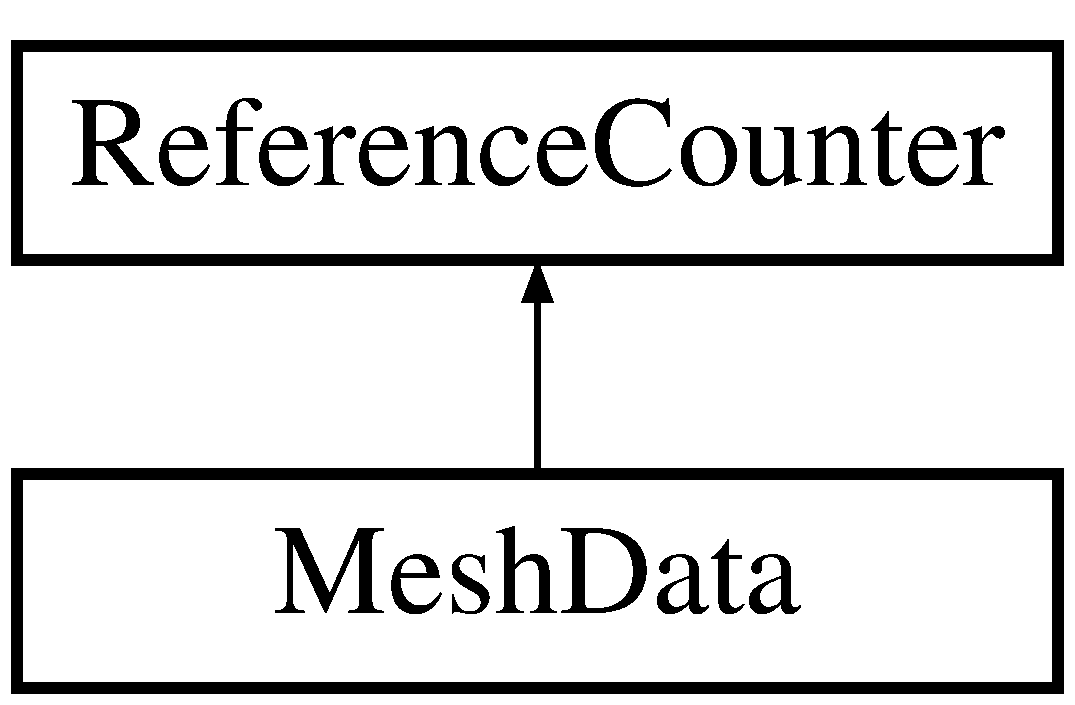
\includegraphics[height=2.000000cm]{class_mesh_data}
\end{center}
\end{figure}
\subsection*{Public Member Functions}
\begin{DoxyCompactItemize}
\item 
\hyperlink{class_mesh_data_ac9808a06ed24bd2478e6bcc69a5be394}{Mesh\+Data} (const \hyperlink{class_indexed_model}{Indexed\+Model} \&model, int material\+Index)
\item 
virtual \hyperlink{class_mesh_data_a6f206f96b3c7ce1d33611fed471729cf}{$\sim$\+Mesh\+Data} ()
\item 
void \hyperlink{class_mesh_data_ae25e7415585357672e370ab74e73dcff}{Draw} () const 
\item 
int \hyperlink{class_mesh_data_a1864908fbe13d34a4f41e749c37a2d63}{Get\+Material\+Index} ()
\end{DoxyCompactItemize}


\subsection{Constructor \& Destructor Documentation}
\hypertarget{class_mesh_data_ac9808a06ed24bd2478e6bcc69a5be394}{}\index{Mesh\+Data@{Mesh\+Data}!Mesh\+Data@{Mesh\+Data}}
\index{Mesh\+Data@{Mesh\+Data}!Mesh\+Data@{Mesh\+Data}}
\subsubsection[{Mesh\+Data(const Indexed\+Model \&model, int material\+Index)}]{\setlength{\rightskip}{0pt plus 5cm}Mesh\+Data\+::\+Mesh\+Data (
\begin{DoxyParamCaption}
\item[{const {\bf Indexed\+Model} \&}]{model, }
\item[{int}]{material\+Index}
\end{DoxyParamCaption}
)}\label{class_mesh_data_ac9808a06ed24bd2478e6bcc69a5be394}
\hypertarget{class_mesh_data_a6f206f96b3c7ce1d33611fed471729cf}{}\index{Mesh\+Data@{Mesh\+Data}!````~Mesh\+Data@{$\sim$\+Mesh\+Data}}
\index{````~Mesh\+Data@{$\sim$\+Mesh\+Data}!Mesh\+Data@{Mesh\+Data}}
\subsubsection[{$\sim$\+Mesh\+Data()}]{\setlength{\rightskip}{0pt plus 5cm}Mesh\+Data\+::$\sim$\+Mesh\+Data (
\begin{DoxyParamCaption}
{}
\end{DoxyParamCaption}
)\hspace{0.3cm}{\ttfamily [virtual]}}\label{class_mesh_data_a6f206f96b3c7ce1d33611fed471729cf}


\subsection{Member Function Documentation}
\hypertarget{class_mesh_data_ae25e7415585357672e370ab74e73dcff}{}\index{Mesh\+Data@{Mesh\+Data}!Draw@{Draw}}
\index{Draw@{Draw}!Mesh\+Data@{Mesh\+Data}}
\subsubsection[{Draw() const }]{\setlength{\rightskip}{0pt plus 5cm}void Mesh\+Data\+::\+Draw (
\begin{DoxyParamCaption}
{}
\end{DoxyParamCaption}
) const}\label{class_mesh_data_ae25e7415585357672e370ab74e73dcff}
\hypertarget{class_mesh_data_a1864908fbe13d34a4f41e749c37a2d63}{}\index{Mesh\+Data@{Mesh\+Data}!Get\+Material\+Index@{Get\+Material\+Index}}
\index{Get\+Material\+Index@{Get\+Material\+Index}!Mesh\+Data@{Mesh\+Data}}
\subsubsection[{Get\+Material\+Index()}]{\setlength{\rightskip}{0pt plus 5cm}int Mesh\+Data\+::\+Get\+Material\+Index (
\begin{DoxyParamCaption}
{}
\end{DoxyParamCaption}
)\hspace{0.3cm}{\ttfamily [inline]}}\label{class_mesh_data_a1864908fbe13d34a4f41e749c37a2d63}


The documentation for this class was generated from the following files\+:\begin{DoxyCompactItemize}
\item 
F\+:/\+Fusion3\+D\+\_\+work/src/rendering/\hyperlink{mesh_8h}{mesh.\+h}\item 
F\+:/\+Fusion3\+D\+\_\+work/src/rendering/\hyperlink{mesh_8cpp}{mesh.\+cpp}\end{DoxyCompactItemize}

\hypertarget{class_physics_engine}{}\section{Physics\+Engine Class Reference}
\label{class_physics_engine}\index{Physics\+Engine@{Physics\+Engine}}


{\ttfamily \#include $<$physics\+Engine.\+h$>$}

\subsection*{Public Member Functions}
\begin{DoxyCompactItemize}
\item 
\hyperlink{class_physics_engine_a7fc9180ea453680df0b863fa157c5b92}{Physics\+Engine} ()
\item 
virtual \hyperlink{class_physics_engine_ade5d084ae76413f23601afde9f38ed61}{$\sim$\+Physics\+Engine} ()
\item 
void \hyperlink{class_physics_engine_a0eef5ab7f12076bd0e065cdd352761bf}{Simulate} (float delta)
\item 
bt\+Discrete\+Dynamics\+World $\ast$ \hyperlink{class_physics_engine_a3055a9cec9a476cd463c6ef1ecd55ec1}{Get\+World} ()
\end{DoxyCompactItemize}


\subsection{Detailed Description}
The \hyperlink{class_physics_engine}{Physics\+Engine} encapsulates all the functions and information necessary to perform a physics simulation. 

\subsection{Constructor \& Destructor Documentation}
\hypertarget{class_physics_engine_a7fc9180ea453680df0b863fa157c5b92}{}\index{Physics\+Engine@{Physics\+Engine}!Physics\+Engine@{Physics\+Engine}}
\index{Physics\+Engine@{Physics\+Engine}!Physics\+Engine@{Physics\+Engine}}
\subsubsection[{Physics\+Engine()}]{\setlength{\rightskip}{0pt plus 5cm}Physics\+Engine\+::\+Physics\+Engine (
\begin{DoxyParamCaption}
{}
\end{DoxyParamCaption}
)\hspace{0.3cm}{\ttfamily [inline]}}\label{class_physics_engine_a7fc9180ea453680df0b863fa157c5b92}
Creates a \hyperlink{class_physics_engine}{Physics\+Engine} in a usable state. \hypertarget{class_physics_engine_ade5d084ae76413f23601afde9f38ed61}{}\index{Physics\+Engine@{Physics\+Engine}!````~Physics\+Engine@{$\sim$\+Physics\+Engine}}
\index{````~Physics\+Engine@{$\sim$\+Physics\+Engine}!Physics\+Engine@{Physics\+Engine}}
\subsubsection[{$\sim$\+Physics\+Engine()}]{\setlength{\rightskip}{0pt plus 5cm}virtual Physics\+Engine\+::$\sim$\+Physics\+Engine (
\begin{DoxyParamCaption}
{}
\end{DoxyParamCaption}
)\hspace{0.3cm}{\ttfamily [inline]}, {\ttfamily [virtual]}}\label{class_physics_engine_ade5d084ae76413f23601afde9f38ed61}


\subsection{Member Function Documentation}
\hypertarget{class_physics_engine_a3055a9cec9a476cd463c6ef1ecd55ec1}{}\index{Physics\+Engine@{Physics\+Engine}!Get\+World@{Get\+World}}
\index{Get\+World@{Get\+World}!Physics\+Engine@{Physics\+Engine}}
\subsubsection[{Get\+World()}]{\setlength{\rightskip}{0pt plus 5cm}bt\+Discrete\+Dynamics\+World$\ast$ Physics\+Engine\+::\+Get\+World (
\begin{DoxyParamCaption}
{}
\end{DoxyParamCaption}
)\hspace{0.3cm}{\ttfamily [inline]}}\label{class_physics_engine_a3055a9cec9a476cd463c6ef1ecd55ec1}
\hypertarget{class_physics_engine_a0eef5ab7f12076bd0e065cdd352761bf}{}\index{Physics\+Engine@{Physics\+Engine}!Simulate@{Simulate}}
\index{Simulate@{Simulate}!Physics\+Engine@{Physics\+Engine}}
\subsubsection[{Simulate(float delta)}]{\setlength{\rightskip}{0pt plus 5cm}void Physics\+Engine\+::\+Simulate (
\begin{DoxyParamCaption}
\item[{float}]{delta}
\end{DoxyParamCaption}
)}\label{class_physics_engine_a0eef5ab7f12076bd0e065cdd352761bf}


The documentation for this class was generated from the following files\+:\begin{DoxyCompactItemize}
\item 
F\+:/\+Fusion3\+D\+\_\+work/src/physics/\hyperlink{physics_engine_8h}{physics\+Engine.\+h}\item 
F\+:/\+Fusion3\+D\+\_\+work/src/physics/\hyperlink{physics_engine_8cpp}{physics\+Engine.\+cpp}\end{DoxyCompactItemize}

\hypertarget{class_physics_object}{}\section{Physics\+Object Class Reference}
\label{class_physics_object}\index{Physics\+Object@{Physics\+Object}}


{\ttfamily \#include $<$physics\+Object.\+h$>$}

\subsection*{Public Member Functions}
\begin{DoxyCompactItemize}
\item 
\hyperlink{class_physics_object_a8f3b1480fd01c6dbc0077e594c0fdb25}{Physics\+Object} (\hyperlink{class_collider}{Collider} $\ast$collider, const \hyperlink{class_vector3f}{Vector3f} \&velocity)
\item 
\hyperlink{class_physics_object_ab0616f80555332ac226ba19a5bc85d9d}{Physics\+Object} (const \hyperlink{class_physics_object}{Physics\+Object} \&other)
\item 
void \hyperlink{class_physics_object_a6bdada2302b80562103a7b5e5e61e700}{operator=} (\hyperlink{class_physics_object}{Physics\+Object} other)
\item 
virtual \hyperlink{class_physics_object_a2172e8b71176e3a54d6a8f5ff15d4178}{$\sim$\+Physics\+Object} ()
\item 
void \hyperlink{class_physics_object_ade8f6f54cfd72a3d6ff081f55121980c}{Integrate} (float delta)
\item 
const \hyperlink{class_vector3f}{Vector3f} \& \hyperlink{class_physics_object_ac76b0fb1e128cda164b7cbb0517e27fe}{Get\+Position} () const 
\item 
const \hyperlink{class_vector3f}{Vector3f} \& \hyperlink{class_physics_object_a3516ba15edaac9d10f5dd900fe7d9d7e}{Get\+Velocity} () const 
\item 
const \hyperlink{class_collider}{Collider} \& \hyperlink{class_physics_object_a05ad38aeee61daebf754530bb41500bb}{Get\+Collider} ()
\item 
void \hyperlink{class_physics_object_a19d90029d890abd4e4f5f69bd48cf0aa}{Set\+Velocity} (const \hyperlink{class_vector3f}{Vector3f} \&velocity)
\end{DoxyCompactItemize}
\subsection*{Static Public Member Functions}
\begin{DoxyCompactItemize}
\item 
static void \hyperlink{class_physics_object_adb7b77e74502546484c55341757cfe7d}{Test} ()
\end{DoxyCompactItemize}


\subsection{Detailed Description}
The \hyperlink{class_physics_object}{Physics\+Object} class represents an object that can be used in a physics engine. 

\subsection{Constructor \& Destructor Documentation}
\hypertarget{class_physics_object_a8f3b1480fd01c6dbc0077e594c0fdb25}{}\index{Physics\+Object@{Physics\+Object}!Physics\+Object@{Physics\+Object}}
\index{Physics\+Object@{Physics\+Object}!Physics\+Object@{Physics\+Object}}
\subsubsection[{Physics\+Object(\+Collider $\ast$collider, const Vector3f \&velocity)}]{\setlength{\rightskip}{0pt plus 5cm}Physics\+Object\+::\+Physics\+Object (
\begin{DoxyParamCaption}
\item[{{\bf Collider} $\ast$}]{collider, }
\item[{const {\bf Vector3f} \&}]{velocity}
\end{DoxyParamCaption}
)\hspace{0.3cm}{\ttfamily [inline]}}\label{class_physics_object_a8f3b1480fd01c6dbc0077e594c0fdb25}
Creates a \hyperlink{class_physics_object}{Physics\+Object} in a usable state.


\begin{DoxyParams}{Parameters}
{\em collider} & A collider representing the shape and position of the object. Should be in allocated memory. \\
\hline
{\em velocity} & How fast this object is moving and in what direction. \\
\hline
\end{DoxyParams}
\hypertarget{class_physics_object_ab0616f80555332ac226ba19a5bc85d9d}{}\index{Physics\+Object@{Physics\+Object}!Physics\+Object@{Physics\+Object}}
\index{Physics\+Object@{Physics\+Object}!Physics\+Object@{Physics\+Object}}
\subsubsection[{Physics\+Object(const Physics\+Object \&other)}]{\setlength{\rightskip}{0pt plus 5cm}Physics\+Object\+::\+Physics\+Object (
\begin{DoxyParamCaption}
\item[{const {\bf Physics\+Object} \&}]{other}
\end{DoxyParamCaption}
)}\label{class_physics_object_ab0616f80555332ac226ba19a5bc85d9d}
\hypertarget{class_physics_object_a2172e8b71176e3a54d6a8f5ff15d4178}{}\index{Physics\+Object@{Physics\+Object}!````~Physics\+Object@{$\sim$\+Physics\+Object}}
\index{````~Physics\+Object@{$\sim$\+Physics\+Object}!Physics\+Object@{Physics\+Object}}
\subsubsection[{$\sim$\+Physics\+Object()}]{\setlength{\rightskip}{0pt plus 5cm}Physics\+Object\+::$\sim$\+Physics\+Object (
\begin{DoxyParamCaption}
{}
\end{DoxyParamCaption}
)\hspace{0.3cm}{\ttfamily [virtual]}}\label{class_physics_object_a2172e8b71176e3a54d6a8f5ff15d4178}


\subsection{Member Function Documentation}
\hypertarget{class_physics_object_a05ad38aeee61daebf754530bb41500bb}{}\index{Physics\+Object@{Physics\+Object}!Get\+Collider@{Get\+Collider}}
\index{Get\+Collider@{Get\+Collider}!Physics\+Object@{Physics\+Object}}
\subsubsection[{Get\+Collider()}]{\setlength{\rightskip}{0pt plus 5cm}const {\bf Collider}\& Physics\+Object\+::\+Get\+Collider (
\begin{DoxyParamCaption}
{}
\end{DoxyParamCaption}
)\hspace{0.3cm}{\ttfamily [inline]}}\label{class_physics_object_a05ad38aeee61daebf754530bb41500bb}
Returns a collider in the position of this object, updating the collider\textquotesingle{}s position if necessary. \hypertarget{class_physics_object_ac76b0fb1e128cda164b7cbb0517e27fe}{}\index{Physics\+Object@{Physics\+Object}!Get\+Position@{Get\+Position}}
\index{Get\+Position@{Get\+Position}!Physics\+Object@{Physics\+Object}}
\subsubsection[{Get\+Position() const }]{\setlength{\rightskip}{0pt plus 5cm}const {\bf Vector3f}\& Physics\+Object\+::\+Get\+Position (
\begin{DoxyParamCaption}
{}
\end{DoxyParamCaption}
) const\hspace{0.3cm}{\ttfamily [inline]}}\label{class_physics_object_ac76b0fb1e128cda164b7cbb0517e27fe}
Basic getter \hypertarget{class_physics_object_a3516ba15edaac9d10f5dd900fe7d9d7e}{}\index{Physics\+Object@{Physics\+Object}!Get\+Velocity@{Get\+Velocity}}
\index{Get\+Velocity@{Get\+Velocity}!Physics\+Object@{Physics\+Object}}
\subsubsection[{Get\+Velocity() const }]{\setlength{\rightskip}{0pt plus 5cm}const {\bf Vector3f}\& Physics\+Object\+::\+Get\+Velocity (
\begin{DoxyParamCaption}
{}
\end{DoxyParamCaption}
) const\hspace{0.3cm}{\ttfamily [inline]}}\label{class_physics_object_a3516ba15edaac9d10f5dd900fe7d9d7e}
Basic getter \hypertarget{class_physics_object_ade8f6f54cfd72a3d6ff081f55121980c}{}\index{Physics\+Object@{Physics\+Object}!Integrate@{Integrate}}
\index{Integrate@{Integrate}!Physics\+Object@{Physics\+Object}}
\subsubsection[{Integrate(float delta)}]{\setlength{\rightskip}{0pt plus 5cm}void Physics\+Object\+::\+Integrate (
\begin{DoxyParamCaption}
\item[{float}]{delta}
\end{DoxyParamCaption}
)}\label{class_physics_object_ade8f6f54cfd72a3d6ff081f55121980c}
Calculate this object\textquotesingle{}s new location and properties after delta seconds


\begin{DoxyParams}{Parameters}
{\em delta} & How much time to simulate. \\
\hline
\end{DoxyParams}
\hypertarget{class_physics_object_a6bdada2302b80562103a7b5e5e61e700}{}\index{Physics\+Object@{Physics\+Object}!operator=@{operator=}}
\index{operator=@{operator=}!Physics\+Object@{Physics\+Object}}
\subsubsection[{operator=(\+Physics\+Object other)}]{\setlength{\rightskip}{0pt plus 5cm}void Physics\+Object\+::operator= (
\begin{DoxyParamCaption}
\item[{{\bf Physics\+Object}}]{other}
\end{DoxyParamCaption}
)}\label{class_physics_object_a6bdada2302b80562103a7b5e5e61e700}
\hypertarget{class_physics_object_a19d90029d890abd4e4f5f69bd48cf0aa}{}\index{Physics\+Object@{Physics\+Object}!Set\+Velocity@{Set\+Velocity}}
\index{Set\+Velocity@{Set\+Velocity}!Physics\+Object@{Physics\+Object}}
\subsubsection[{Set\+Velocity(const Vector3f \&velocity)}]{\setlength{\rightskip}{0pt plus 5cm}void Physics\+Object\+::\+Set\+Velocity (
\begin{DoxyParamCaption}
\item[{const {\bf Vector3f} \&}]{velocity}
\end{DoxyParamCaption}
)\hspace{0.3cm}{\ttfamily [inline]}}\label{class_physics_object_a19d90029d890abd4e4f5f69bd48cf0aa}
Basic setter \hypertarget{class_physics_object_adb7b77e74502546484c55341757cfe7d}{}\index{Physics\+Object@{Physics\+Object}!Test@{Test}}
\index{Test@{Test}!Physics\+Object@{Physics\+Object}}
\subsubsection[{Test()}]{\setlength{\rightskip}{0pt plus 5cm}void Physics\+Object\+::\+Test (
\begin{DoxyParamCaption}
{}
\end{DoxyParamCaption}
)\hspace{0.3cm}{\ttfamily [static]}}\label{class_physics_object_adb7b77e74502546484c55341757cfe7d}
Performs a Unit Test of this class 

The documentation for this class was generated from the following files\+:\begin{DoxyCompactItemize}
\item 
F\+:/\+Fusion3\+D\+\_\+work/src/physics/\hyperlink{physics_object_8h}{physics\+Object.\+h}\item 
F\+:/\+Fusion3\+D\+\_\+work/src/physics/\hyperlink{physics_object_8cpp}{physics\+Object.\+cpp}\end{DoxyCompactItemize}

\hypertarget{class_physics_object_component}{}\section{Physics\+Object\+Component Class Reference}
\label{class_physics_object_component}\index{Physics\+Object\+Component@{Physics\+Object\+Component}}


{\ttfamily \#include $<$physics\+Object\+Component.\+h$>$}

Inheritance diagram for Physics\+Object\+Component\+:\begin{figure}[H]
\begin{center}
\leavevmode
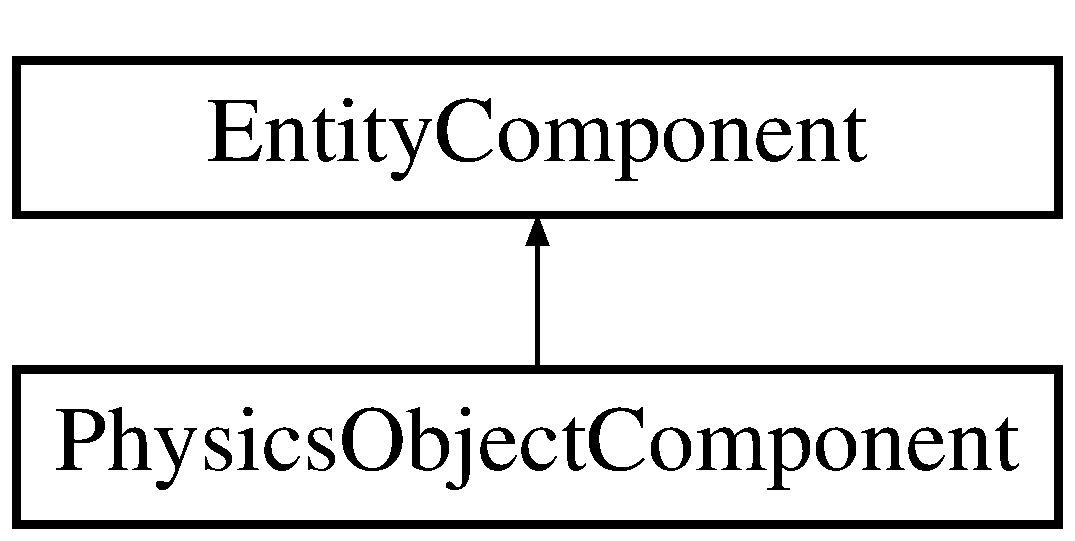
\includegraphics[height=2.000000cm]{class_physics_object_component}
\end{center}
\end{figure}
\subsection*{Public Member Functions}
\begin{DoxyCompactItemize}
\item 
\hyperlink{class_physics_object_component_a3411bc1cdf04a16461a046e4ca63ca9a}{Physics\+Object\+Component} (bt\+Collision\+Shape $\ast$shape, float mass=0.\+0f, bool calc\+Inertia=true, Vector3f inertia=\+Vector3f(0, 0, 0))
\item 
virtual \hyperlink{class_physics_object_component_ae850bb2f556a14a79e22bca7d2999dee}{$\sim$\+Physics\+Object\+Component} ()
\item 
virtual void \hyperlink{class_physics_object_component_a9383128bd0b76d2289664053bca5c770}{Init} ()
\item 
virtual void \hyperlink{class_physics_object_component_ab06a52c369ed9cef4852309a0e97fa1c}{Update} (float delta)
\item 
bt\+Rigid\+Body $\ast$ \hyperlink{class_physics_object_component_af9a3bf0a2ea6aaf4c69a6c5e7dca5a73}{Get\+Body} ()
\item 
void \hyperlink{class_physics_object_component_a7bde28d4e0e1c44cd95e2870d03d917a}{Update\+Transform} ()
\end{DoxyCompactItemize}


\subsection{Constructor \& Destructor Documentation}
\hypertarget{class_physics_object_component_a3411bc1cdf04a16461a046e4ca63ca9a}{}\index{Physics\+Object\+Component@{Physics\+Object\+Component}!Physics\+Object\+Component@{Physics\+Object\+Component}}
\index{Physics\+Object\+Component@{Physics\+Object\+Component}!Physics\+Object\+Component@{Physics\+Object\+Component}}
\subsubsection[{Physics\+Object\+Component(bt\+Collision\+Shape $\ast$shape, float mass=0.\+0f, bool calc\+Inertia=true, Vector3f inertia=\+Vector3f(0, 0, 0))}]{\setlength{\rightskip}{0pt plus 5cm}Physics\+Object\+Component\+::\+Physics\+Object\+Component (
\begin{DoxyParamCaption}
\item[{bt\+Collision\+Shape $\ast$}]{shape, }
\item[{float}]{mass = {\ttfamily 0.0f}, }
\item[{bool}]{calc\+Inertia = {\ttfamily true}, }
\item[{{\bf Vector3f}}]{inertia = {\ttfamily {\bf Vector3f}(0,0,0)}}
\end{DoxyParamCaption}
)\hspace{0.3cm}{\ttfamily [inline]}}\label{class_physics_object_component_a3411bc1cdf04a16461a046e4ca63ca9a}
\hypertarget{class_physics_object_component_ae850bb2f556a14a79e22bca7d2999dee}{}\index{Physics\+Object\+Component@{Physics\+Object\+Component}!````~Physics\+Object\+Component@{$\sim$\+Physics\+Object\+Component}}
\index{````~Physics\+Object\+Component@{$\sim$\+Physics\+Object\+Component}!Physics\+Object\+Component@{Physics\+Object\+Component}}
\subsubsection[{$\sim$\+Physics\+Object\+Component()}]{\setlength{\rightskip}{0pt plus 5cm}virtual Physics\+Object\+Component\+::$\sim$\+Physics\+Object\+Component (
\begin{DoxyParamCaption}
{}
\end{DoxyParamCaption}
)\hspace{0.3cm}{\ttfamily [inline]}, {\ttfamily [virtual]}}\label{class_physics_object_component_ae850bb2f556a14a79e22bca7d2999dee}


\subsection{Member Function Documentation}
\hypertarget{class_physics_object_component_af9a3bf0a2ea6aaf4c69a6c5e7dca5a73}{}\index{Physics\+Object\+Component@{Physics\+Object\+Component}!Get\+Body@{Get\+Body}}
\index{Get\+Body@{Get\+Body}!Physics\+Object\+Component@{Physics\+Object\+Component}}
\subsubsection[{Get\+Body()}]{\setlength{\rightskip}{0pt plus 5cm}bt\+Rigid\+Body$\ast$ Physics\+Object\+Component\+::\+Get\+Body (
\begin{DoxyParamCaption}
{}
\end{DoxyParamCaption}
)\hspace{0.3cm}{\ttfamily [inline]}}\label{class_physics_object_component_af9a3bf0a2ea6aaf4c69a6c5e7dca5a73}
\hypertarget{class_physics_object_component_a9383128bd0b76d2289664053bca5c770}{}\index{Physics\+Object\+Component@{Physics\+Object\+Component}!Init@{Init}}
\index{Init@{Init}!Physics\+Object\+Component@{Physics\+Object\+Component}}
\subsubsection[{Init()}]{\setlength{\rightskip}{0pt plus 5cm}virtual void Physics\+Object\+Component\+::\+Init (
\begin{DoxyParamCaption}
{}
\end{DoxyParamCaption}
)\hspace{0.3cm}{\ttfamily [inline]}, {\ttfamily [virtual]}}\label{class_physics_object_component_a9383128bd0b76d2289664053bca5c770}


Reimplemented from \hyperlink{class_entity_component_ae8878fb678135211d30c6ef23d8447e7}{Entity\+Component}.

\hypertarget{class_physics_object_component_ab06a52c369ed9cef4852309a0e97fa1c}{}\index{Physics\+Object\+Component@{Physics\+Object\+Component}!Update@{Update}}
\index{Update@{Update}!Physics\+Object\+Component@{Physics\+Object\+Component}}
\subsubsection[{Update(float delta)}]{\setlength{\rightskip}{0pt plus 5cm}virtual void Physics\+Object\+Component\+::\+Update (
\begin{DoxyParamCaption}
\item[{float}]{delta}
\end{DoxyParamCaption}
)\hspace{0.3cm}{\ttfamily [inline]}, {\ttfamily [virtual]}}\label{class_physics_object_component_ab06a52c369ed9cef4852309a0e97fa1c}


Reimplemented from \hyperlink{class_entity_component_aa73f3be22173ada22f997825f29aa918}{Entity\+Component}.

\hypertarget{class_physics_object_component_a7bde28d4e0e1c44cd95e2870d03d917a}{}\index{Physics\+Object\+Component@{Physics\+Object\+Component}!Update\+Transform@{Update\+Transform}}
\index{Update\+Transform@{Update\+Transform}!Physics\+Object\+Component@{Physics\+Object\+Component}}
\subsubsection[{Update\+Transform()}]{\setlength{\rightskip}{0pt plus 5cm}void Physics\+Object\+Component\+::\+Update\+Transform (
\begin{DoxyParamCaption}
{}
\end{DoxyParamCaption}
)\hspace{0.3cm}{\ttfamily [inline]}}\label{class_physics_object_component_a7bde28d4e0e1c44cd95e2870d03d917a}


The documentation for this class was generated from the following file\+:\begin{DoxyCompactItemize}
\item 
F\+:/\+Fusion3\+D\+\_\+work/src/components/\hyperlink{physics_object_component_8h}{physics\+Object\+Component.\+h}\end{DoxyCompactItemize}

\hypertarget{structpic__packet__t}{}\section{pic\+\_\+packet\+\_\+t Struct Reference}
\label{structpic__packet__t}\index{pic\+\_\+packet\+\_\+t@{pic\+\_\+packet\+\_\+t}}
\subsection*{Public Attributes}
\begin{DoxyCompactItemize}
\item 
\hyperlink{stb__image_8h_a28eb51a1512ce382ee50f20e1d04d50d}{stbi\+\_\+uc} \hyperlink{structpic__packet__t_ad33021e40c272a20d89bdcceabb20a71}{size}
\item 
\hyperlink{stb__image_8h_a28eb51a1512ce382ee50f20e1d04d50d}{stbi\+\_\+uc} \hyperlink{structpic__packet__t_abc346cfdcff43f051830335296f14aaa}{type}
\item 
\hyperlink{stb__image_8h_a28eb51a1512ce382ee50f20e1d04d50d}{stbi\+\_\+uc} \hyperlink{structpic__packet__t_af64f17c991495f3f3baf6782a253f7cc}{channel}
\end{DoxyCompactItemize}


\subsection{Member Data Documentation}
\hypertarget{structpic__packet__t_af64f17c991495f3f3baf6782a253f7cc}{}\index{pic\+\_\+packet\+\_\+t@{pic\+\_\+packet\+\_\+t}!channel@{channel}}
\index{channel@{channel}!pic\+\_\+packet\+\_\+t@{pic\+\_\+packet\+\_\+t}}
\subsubsection[{channel}]{\setlength{\rightskip}{0pt plus 5cm}{\bf stbi\+\_\+uc} pic\+\_\+packet\+\_\+t\+::channel}\label{structpic__packet__t_af64f17c991495f3f3baf6782a253f7cc}
\hypertarget{structpic__packet__t_ad33021e40c272a20d89bdcceabb20a71}{}\index{pic\+\_\+packet\+\_\+t@{pic\+\_\+packet\+\_\+t}!size@{size}}
\index{size@{size}!pic\+\_\+packet\+\_\+t@{pic\+\_\+packet\+\_\+t}}
\subsubsection[{size}]{\setlength{\rightskip}{0pt plus 5cm}{\bf stbi\+\_\+uc} pic\+\_\+packet\+\_\+t\+::size}\label{structpic__packet__t_ad33021e40c272a20d89bdcceabb20a71}
\hypertarget{structpic__packet__t_abc346cfdcff43f051830335296f14aaa}{}\index{pic\+\_\+packet\+\_\+t@{pic\+\_\+packet\+\_\+t}!type@{type}}
\index{type@{type}!pic\+\_\+packet\+\_\+t@{pic\+\_\+packet\+\_\+t}}
\subsubsection[{type}]{\setlength{\rightskip}{0pt plus 5cm}{\bf stbi\+\_\+uc} pic\+\_\+packet\+\_\+t\+::type}\label{structpic__packet__t_abc346cfdcff43f051830335296f14aaa}


The documentation for this struct was generated from the following file\+:\begin{DoxyCompactItemize}
\item 
F\+:/\+Fusion3\+D\+\_\+work/src/static\+Libs/\hyperlink{stb__image_8c}{stb\+\_\+image.\+c}\end{DoxyCompactItemize}

\hypertarget{class_plane}{}\section{Plane Class Reference}
\label{class_plane}\index{Plane@{Plane}}


{\ttfamily \#include $<$plane.\+h$>$}

\subsection*{Public Member Functions}
\begin{DoxyCompactItemize}
\item 
\hyperlink{class_plane_a51ccb4a1b7d2934a30fc50f96559d2fd}{Plane} (const \hyperlink{class_vector3f}{Vector3f} \&normal, float distance)
\item 
\hyperlink{class_plane}{Plane} \hyperlink{class_plane_a55f5df21e132b0abe1e0884142955404}{Normalized} () const 
\item 
\hyperlink{class_intersect_data}{Intersect\+Data} \hyperlink{class_plane_a39d79adca4637fe29b00fcb82571515d}{Intersect\+Sphere} (const \hyperlink{class_bounding_sphere}{Bounding\+Sphere} \&other) const 
\item 
const \hyperlink{class_vector3f}{Vector3f} \& \hyperlink{class_plane_aa3238680f7e7afa2d39270797d9398b4}{Get\+Normal} () const 
\item 
float \hyperlink{class_plane_a180076c8616efa9ea205ac17a6c5bebf}{Get\+Distance} () const 
\end{DoxyCompactItemize}
\subsection*{Static Public Member Functions}
\begin{DoxyCompactItemize}
\item 
static void \hyperlink{class_plane_a5ae751326c9dbeae32d783664801f640}{Test} ()
\end{DoxyCompactItemize}


\subsection{Detailed Description}
The \hyperlink{class_plane}{Plane} class represents an infinitely large plane that can be used as a collider in a physics engine. 

\subsection{Constructor \& Destructor Documentation}
\hypertarget{class_plane_a51ccb4a1b7d2934a30fc50f96559d2fd}{}\index{Plane@{Plane}!Plane@{Plane}}
\index{Plane@{Plane}!Plane@{Plane}}
\subsubsection[{Plane(const Vector3f \&normal, float distance)}]{\setlength{\rightskip}{0pt plus 5cm}Plane\+::\+Plane (
\begin{DoxyParamCaption}
\item[{const {\bf Vector3f} \&}]{normal, }
\item[{float}]{distance}
\end{DoxyParamCaption}
)\hspace{0.3cm}{\ttfamily [inline]}}\label{class_plane_a51ccb4a1b7d2934a30fc50f96559d2fd}
Creates a \hyperlink{class_plane}{Plane} in a usable state.


\begin{DoxyParams}{Parameters}
{\em normal} & The \char`\"{}up\char`\"{} direction from the plane\textquotesingle{}s surface. \\
\hline
{\em distance} & The distance to the plane from the world origin along the normal \\
\hline
\end{DoxyParams}


\subsection{Member Function Documentation}
\hypertarget{class_plane_a180076c8616efa9ea205ac17a6c5bebf}{}\index{Plane@{Plane}!Get\+Distance@{Get\+Distance}}
\index{Get\+Distance@{Get\+Distance}!Plane@{Plane}}
\subsubsection[{Get\+Distance() const }]{\setlength{\rightskip}{0pt plus 5cm}float Plane\+::\+Get\+Distance (
\begin{DoxyParamCaption}
{}
\end{DoxyParamCaption}
) const\hspace{0.3cm}{\ttfamily [inline]}}\label{class_plane_a180076c8616efa9ea205ac17a6c5bebf}
\hypertarget{class_plane_aa3238680f7e7afa2d39270797d9398b4}{}\index{Plane@{Plane}!Get\+Normal@{Get\+Normal}}
\index{Get\+Normal@{Get\+Normal}!Plane@{Plane}}
\subsubsection[{Get\+Normal() const }]{\setlength{\rightskip}{0pt plus 5cm}const {\bf Vector3f}\& Plane\+::\+Get\+Normal (
\begin{DoxyParamCaption}
{}
\end{DoxyParamCaption}
) const\hspace{0.3cm}{\ttfamily [inline]}}\label{class_plane_aa3238680f7e7afa2d39270797d9398b4}
\hypertarget{class_plane_a39d79adca4637fe29b00fcb82571515d}{}\index{Plane@{Plane}!Intersect\+Sphere@{Intersect\+Sphere}}
\index{Intersect\+Sphere@{Intersect\+Sphere}!Plane@{Plane}}
\subsubsection[{Intersect\+Sphere(const Bounding\+Sphere \&other) const }]{\setlength{\rightskip}{0pt plus 5cm}{\bf Intersect\+Data} Plane\+::\+Intersect\+Sphere (
\begin{DoxyParamCaption}
\item[{const {\bf Bounding\+Sphere} \&}]{other}
\end{DoxyParamCaption}
) const}\label{class_plane_a39d79adca4637fe29b00fcb82571515d}
Computes information about if this \hyperlink{class_plane}{Plane} intersects a Sphere.


\begin{DoxyParams}{Parameters}
{\em other} & The Sphere that\textquotesingle{}s being tested for intersection with this \hyperlink{class_plane}{Plane}. \\
\hline
\end{DoxyParams}
\hypertarget{class_plane_a55f5df21e132b0abe1e0884142955404}{}\index{Plane@{Plane}!Normalized@{Normalized}}
\index{Normalized@{Normalized}!Plane@{Plane}}
\subsubsection[{Normalized() const }]{\setlength{\rightskip}{0pt plus 5cm}{\bf Plane} Plane\+::\+Normalized (
\begin{DoxyParamCaption}
{}
\end{DoxyParamCaption}
) const}\label{class_plane_a55f5df21e132b0abe1e0884142955404}
Creates an equivalent plane with a normal at unit length and distance adjusted accordingly. \hypertarget{class_plane_a5ae751326c9dbeae32d783664801f640}{}\index{Plane@{Plane}!Test@{Test}}
\index{Test@{Test}!Plane@{Plane}}
\subsubsection[{Test()}]{\setlength{\rightskip}{0pt plus 5cm}void Plane\+::\+Test (
\begin{DoxyParamCaption}
{}
\end{DoxyParamCaption}
)\hspace{0.3cm}{\ttfamily [static]}}\label{class_plane_a5ae751326c9dbeae32d783664801f640}
Performs a Unit Test of this class 

The documentation for this class was generated from the following files\+:\begin{DoxyCompactItemize}
\item 
F\+:/\+Fusion3\+D\+\_\+work/src/physics/\hyperlink{plane_8h}{plane.\+h}\item 
F\+:/\+Fusion3\+D\+\_\+work/src/physics/\hyperlink{plane_8cpp}{plane.\+cpp}\end{DoxyCompactItemize}

\hypertarget{structpng}{}\section{png Struct Reference}
\label{structpng}\index{png@{png}}
\subsection*{Public Attributes}
\begin{DoxyCompactItemize}
\item 
\hyperlink{structstbi}{stbi} $\ast$ \hyperlink{structpng_a77d3bfd0ae8f598a475317ed39e78fd0}{s}
\item 
\hyperlink{stb__image_8c_adde6aaee8457bee49c2a92621fe22b79}{uint8} $\ast$ \hyperlink{structpng_a5cd944fdf0f0417a344bcc538ed98ed6}{idata}
\item 
\hyperlink{stb__image_8c_adde6aaee8457bee49c2a92621fe22b79}{uint8} $\ast$ \hyperlink{structpng_a474dd0da8ac0347924e68f5de7e68c55}{expanded}
\item 
\hyperlink{stb__image_8c_adde6aaee8457bee49c2a92621fe22b79}{uint8} $\ast$ \hyperlink{structpng_ada33c39620ad9a647c088c40d21887f6}{out}
\end{DoxyCompactItemize}


\subsection{Member Data Documentation}
\hypertarget{structpng_a474dd0da8ac0347924e68f5de7e68c55}{}\index{png@{png}!expanded@{expanded}}
\index{expanded@{expanded}!png@{png}}
\subsubsection[{expanded}]{\setlength{\rightskip}{0pt plus 5cm}{\bf uint8} $\ast$ png\+::expanded}\label{structpng_a474dd0da8ac0347924e68f5de7e68c55}
\hypertarget{structpng_a5cd944fdf0f0417a344bcc538ed98ed6}{}\index{png@{png}!idata@{idata}}
\index{idata@{idata}!png@{png}}
\subsubsection[{idata}]{\setlength{\rightskip}{0pt plus 5cm}{\bf uint8}$\ast$ png\+::idata}\label{structpng_a5cd944fdf0f0417a344bcc538ed98ed6}
\hypertarget{structpng_ada33c39620ad9a647c088c40d21887f6}{}\index{png@{png}!out@{out}}
\index{out@{out}!png@{png}}
\subsubsection[{out}]{\setlength{\rightskip}{0pt plus 5cm}{\bf uint8} $\ast$ png\+::out}\label{structpng_ada33c39620ad9a647c088c40d21887f6}
\hypertarget{structpng_a77d3bfd0ae8f598a475317ed39e78fd0}{}\index{png@{png}!s@{s}}
\index{s@{s}!png@{png}}
\subsubsection[{s}]{\setlength{\rightskip}{0pt plus 5cm}{\bf stbi}$\ast$ png\+::s}\label{structpng_a77d3bfd0ae8f598a475317ed39e78fd0}


The documentation for this struct was generated from the following file\+:\begin{DoxyCompactItemize}
\item 
F\+:/\+Fusion3\+D\+\_\+work/src/static\+Libs/\hyperlink{stb__image_8c}{stb\+\_\+image.\+c}\end{DoxyCompactItemize}

\hypertarget{class_profile_timer}{}\section{Profile\+Timer Class Reference}
\label{class_profile_timer}\index{Profile\+Timer@{Profile\+Timer}}


{\ttfamily \#include $<$profiling.\+h$>$}

\subsection*{Public Member Functions}
\begin{DoxyCompactItemize}
\item 
\hyperlink{class_profile_timer_ae48cfec1a2159924da8568b289d6e412}{Profile\+Timer} ()
\item 
void \hyperlink{class_profile_timer_a490107f6375f94483ec46db598f622ed}{Start\+Invocation} ()
\item 
void \hyperlink{class_profile_timer_af7037476ec46701a331459056537ce9c}{Stop\+Invocation} ()
\item 
double \hyperlink{class_profile_timer_ac88dc847d8231eccc7e8c0c5053d8750}{Display\+And\+Reset} (const std\+::string \&message, double divisor=0, int displayed\+Message\+Length=40)
\item 
double \hyperlink{class_profile_timer_a27fe1dd5edf793ce784f2382573fe030}{Get\+Time\+And\+Reset} (double divisor=0)
\end{DoxyCompactItemize}


\subsection{Constructor \& Destructor Documentation}
\hypertarget{class_profile_timer_ae48cfec1a2159924da8568b289d6e412}{}\index{Profile\+Timer@{Profile\+Timer}!Profile\+Timer@{Profile\+Timer}}
\index{Profile\+Timer@{Profile\+Timer}!Profile\+Timer@{Profile\+Timer}}
\subsubsection[{Profile\+Timer()}]{\setlength{\rightskip}{0pt plus 5cm}Profile\+Timer\+::\+Profile\+Timer (
\begin{DoxyParamCaption}
{}
\end{DoxyParamCaption}
)\hspace{0.3cm}{\ttfamily [inline]}}\label{class_profile_timer_ae48cfec1a2159924da8568b289d6e412}


\subsection{Member Function Documentation}
\hypertarget{class_profile_timer_ac88dc847d8231eccc7e8c0c5053d8750}{}\index{Profile\+Timer@{Profile\+Timer}!Display\+And\+Reset@{Display\+And\+Reset}}
\index{Display\+And\+Reset@{Display\+And\+Reset}!Profile\+Timer@{Profile\+Timer}}
\subsubsection[{Display\+And\+Reset(const std\+::string \&message, double divisor=0, int displayed\+Message\+Length=40)}]{\setlength{\rightskip}{0pt plus 5cm}double Profile\+Timer\+::\+Display\+And\+Reset (
\begin{DoxyParamCaption}
\item[{const std\+::string \&}]{message, }
\item[{double}]{divisor = {\ttfamily 0}, }
\item[{int}]{displayed\+Message\+Length = {\ttfamily 40}}
\end{DoxyParamCaption}
)}\label{class_profile_timer_ac88dc847d8231eccc7e8c0c5053d8750}
\hypertarget{class_profile_timer_a27fe1dd5edf793ce784f2382573fe030}{}\index{Profile\+Timer@{Profile\+Timer}!Get\+Time\+And\+Reset@{Get\+Time\+And\+Reset}}
\index{Get\+Time\+And\+Reset@{Get\+Time\+And\+Reset}!Profile\+Timer@{Profile\+Timer}}
\subsubsection[{Get\+Time\+And\+Reset(double divisor=0)}]{\setlength{\rightskip}{0pt plus 5cm}double Profile\+Timer\+::\+Get\+Time\+And\+Reset (
\begin{DoxyParamCaption}
\item[{double}]{divisor = {\ttfamily 0}}
\end{DoxyParamCaption}
)}\label{class_profile_timer_a27fe1dd5edf793ce784f2382573fe030}
\hypertarget{class_profile_timer_a490107f6375f94483ec46db598f622ed}{}\index{Profile\+Timer@{Profile\+Timer}!Start\+Invocation@{Start\+Invocation}}
\index{Start\+Invocation@{Start\+Invocation}!Profile\+Timer@{Profile\+Timer}}
\subsubsection[{Start\+Invocation()}]{\setlength{\rightskip}{0pt plus 5cm}void Profile\+Timer\+::\+Start\+Invocation (
\begin{DoxyParamCaption}
{}
\end{DoxyParamCaption}
)}\label{class_profile_timer_a490107f6375f94483ec46db598f622ed}
\hypertarget{class_profile_timer_af7037476ec46701a331459056537ce9c}{}\index{Profile\+Timer@{Profile\+Timer}!Stop\+Invocation@{Stop\+Invocation}}
\index{Stop\+Invocation@{Stop\+Invocation}!Profile\+Timer@{Profile\+Timer}}
\subsubsection[{Stop\+Invocation()}]{\setlength{\rightskip}{0pt plus 5cm}void Profile\+Timer\+::\+Stop\+Invocation (
\begin{DoxyParamCaption}
{}
\end{DoxyParamCaption}
)}\label{class_profile_timer_af7037476ec46701a331459056537ce9c}


The documentation for this class was generated from the following files\+:\begin{DoxyCompactItemize}
\item 
F\+:/\+Fusion3\+D\+\_\+work/src/core/\hyperlink{profiling_8h}{profiling.\+h}\item 
F\+:/\+Fusion3\+D\+\_\+work/src/core/\hyperlink{profiling_8cpp}{profiling.\+cpp}\end{DoxyCompactItemize}

\hypertarget{class_program}{}\section{Program Class Reference}
\label{class_program}\index{Program@{Program}}


{\ttfamily \#include $<$program\+Component.\+h$>$}

\subsection*{Public Member Functions}
\begin{DoxyCompactItemize}
\item 
\hyperlink{class_program_aaefaa0df08f3484476fc4d61e97acbdc}{Program} ()
\item 
virtual \hyperlink{class_program_a2df844d46504a414498c2140de94bfef}{$\sim$\+Program} ()
\item 
virtual int \hyperlink{class_program_adb84adf35f67b0b49e2647a378480e93}{Init} ()
\item 
virtual int \hyperlink{class_program_aca3103ac8fc4b4b982b5f7e70df30584}{Process\+Input} (const \hyperlink{class_input}{Input} \&input, float delta)
\item 
virtual int \hyperlink{class_program_a0398d9957f8da7fb37ea77acf8bac342}{Update} (float delta)
\item 
virtual int \hyperlink{class_program_a79eb729b98fa474234fdbe4404d2f2a9}{Render} (const \hyperlink{class_shader}{Shader} \&shader, const \hyperlink{class_rendering_engine}{Rendering\+Engine} \&rendering\+Engine, const \hyperlink{class_camera}{Camera} \&camera) const 
\item 
virtual int \hyperlink{class_program_a29cf518215935cac6db281732f876871}{Render} (const \hyperlink{class_shader}{Shader} \&shader, const \hyperlink{class_rendering_engine}{Rendering\+Engine} \&rendering\+Engine, const \hyperlink{class_camera}{Camera} \&camera)
\item 
virtual std\+::string \hyperlink{class_program_aacda59ac678fb196f9d5cf89e9a42885}{Get\+Program\+Name} ()
\item 
virtual std\+::string \hyperlink{class_program_a97d6284ddd0a4abec1041b9fca178829}{Get\+Latest\+Error} ()
\item 
void \hyperlink{class_program_ad57322336bab7b5ec5b68857ddfe74ee}{Set\+Parent} (\hyperlink{class_entity}{Entity} $\ast$parent)
\end{DoxyCompactItemize}
\subsection*{Protected Member Functions}
\begin{DoxyCompactItemize}
\item 
virtual void \hyperlink{class_program_aee307e293b04d3e47218d30d6871e6f7}{Push\+Error} (std\+::string err)
\item 
\hyperlink{class_entity}{Entity} $\ast$ \hyperlink{class_program_a58a5d26f7d63df786edacb2332c9e594}{Get\+Parent} ()
\end{DoxyCompactItemize}
\subsection*{Protected Attributes}
\begin{DoxyCompactItemize}
\item 
std\+::set$<$ std\+::string $>$ \hyperlink{class_program_acacd819e20737d226d82e73a733e8c27}{m\+\_\+error}
\end{DoxyCompactItemize}


\subsection{Constructor \& Destructor Documentation}
\hypertarget{class_program_aaefaa0df08f3484476fc4d61e97acbdc}{}\index{Program@{Program}!Program@{Program}}
\index{Program@{Program}!Program@{Program}}
\subsubsection[{Program()}]{\setlength{\rightskip}{0pt plus 5cm}Program\+::\+Program (
\begin{DoxyParamCaption}
{}
\end{DoxyParamCaption}
)\hspace{0.3cm}{\ttfamily [inline]}}\label{class_program_aaefaa0df08f3484476fc4d61e97acbdc}
\hypertarget{class_program_a2df844d46504a414498c2140de94bfef}{}\index{Program@{Program}!````~Program@{$\sim$\+Program}}
\index{````~Program@{$\sim$\+Program}!Program@{Program}}
\subsubsection[{$\sim$\+Program()}]{\setlength{\rightskip}{0pt plus 5cm}virtual Program\+::$\sim$\+Program (
\begin{DoxyParamCaption}
{}
\end{DoxyParamCaption}
)\hspace{0.3cm}{\ttfamily [inline]}, {\ttfamily [virtual]}}\label{class_program_a2df844d46504a414498c2140de94bfef}


\subsection{Member Function Documentation}
\hypertarget{class_program_a97d6284ddd0a4abec1041b9fca178829}{}\index{Program@{Program}!Get\+Latest\+Error@{Get\+Latest\+Error}}
\index{Get\+Latest\+Error@{Get\+Latest\+Error}!Program@{Program}}
\subsubsection[{Get\+Latest\+Error()}]{\setlength{\rightskip}{0pt plus 5cm}virtual std\+::string Program\+::\+Get\+Latest\+Error (
\begin{DoxyParamCaption}
{}
\end{DoxyParamCaption}
)\hspace{0.3cm}{\ttfamily [inline]}, {\ttfamily [virtual]}}\label{class_program_a97d6284ddd0a4abec1041b9fca178829}
\hypertarget{class_program_a58a5d26f7d63df786edacb2332c9e594}{}\index{Program@{Program}!Get\+Parent@{Get\+Parent}}
\index{Get\+Parent@{Get\+Parent}!Program@{Program}}
\subsubsection[{Get\+Parent()}]{\setlength{\rightskip}{0pt plus 5cm}{\bf Entity}$\ast$ Program\+::\+Get\+Parent (
\begin{DoxyParamCaption}
{}
\end{DoxyParamCaption}
)\hspace{0.3cm}{\ttfamily [inline]}, {\ttfamily [protected]}}\label{class_program_a58a5d26f7d63df786edacb2332c9e594}
\hypertarget{class_program_aacda59ac678fb196f9d5cf89e9a42885}{}\index{Program@{Program}!Get\+Program\+Name@{Get\+Program\+Name}}
\index{Get\+Program\+Name@{Get\+Program\+Name}!Program@{Program}}
\subsubsection[{Get\+Program\+Name()}]{\setlength{\rightskip}{0pt plus 5cm}virtual std\+::string Program\+::\+Get\+Program\+Name (
\begin{DoxyParamCaption}
{}
\end{DoxyParamCaption}
)\hspace{0.3cm}{\ttfamily [inline]}, {\ttfamily [virtual]}}\label{class_program_aacda59ac678fb196f9d5cf89e9a42885}
\hypertarget{class_program_adb84adf35f67b0b49e2647a378480e93}{}\index{Program@{Program}!Init@{Init}}
\index{Init@{Init}!Program@{Program}}
\subsubsection[{Init()}]{\setlength{\rightskip}{0pt plus 5cm}virtual int Program\+::\+Init (
\begin{DoxyParamCaption}
{}
\end{DoxyParamCaption}
)\hspace{0.3cm}{\ttfamily [inline]}, {\ttfamily [virtual]}}\label{class_program_adb84adf35f67b0b49e2647a378480e93}
\hypertarget{class_program_aca3103ac8fc4b4b982b5f7e70df30584}{}\index{Program@{Program}!Process\+Input@{Process\+Input}}
\index{Process\+Input@{Process\+Input}!Program@{Program}}
\subsubsection[{Process\+Input(const Input \&input, float delta)}]{\setlength{\rightskip}{0pt plus 5cm}virtual int Program\+::\+Process\+Input (
\begin{DoxyParamCaption}
\item[{const {\bf Input} \&}]{input, }
\item[{float}]{delta}
\end{DoxyParamCaption}
)\hspace{0.3cm}{\ttfamily [inline]}, {\ttfamily [virtual]}}\label{class_program_aca3103ac8fc4b4b982b5f7e70df30584}
\hypertarget{class_program_aee307e293b04d3e47218d30d6871e6f7}{}\index{Program@{Program}!Push\+Error@{Push\+Error}}
\index{Push\+Error@{Push\+Error}!Program@{Program}}
\subsubsection[{Push\+Error(std\+::string err)}]{\setlength{\rightskip}{0pt plus 5cm}virtual void Program\+::\+Push\+Error (
\begin{DoxyParamCaption}
\item[{std\+::string}]{err}
\end{DoxyParamCaption}
)\hspace{0.3cm}{\ttfamily [inline]}, {\ttfamily [protected]}, {\ttfamily [virtual]}}\label{class_program_aee307e293b04d3e47218d30d6871e6f7}
\hypertarget{class_program_a79eb729b98fa474234fdbe4404d2f2a9}{}\index{Program@{Program}!Render@{Render}}
\index{Render@{Render}!Program@{Program}}
\subsubsection[{Render(const Shader \&shader, const Rendering\+Engine \&rendering\+Engine, const Camera \&camera) const }]{\setlength{\rightskip}{0pt plus 5cm}virtual int Program\+::\+Render (
\begin{DoxyParamCaption}
\item[{const {\bf Shader} \&}]{shader, }
\item[{const {\bf Rendering\+Engine} \&}]{rendering\+Engine, }
\item[{const {\bf Camera} \&}]{camera}
\end{DoxyParamCaption}
) const\hspace{0.3cm}{\ttfamily [inline]}, {\ttfamily [virtual]}}\label{class_program_a79eb729b98fa474234fdbe4404d2f2a9}
\hypertarget{class_program_a29cf518215935cac6db281732f876871}{}\index{Program@{Program}!Render@{Render}}
\index{Render@{Render}!Program@{Program}}
\subsubsection[{Render(const Shader \&shader, const Rendering\+Engine \&rendering\+Engine, const Camera \&camera)}]{\setlength{\rightskip}{0pt plus 5cm}virtual int Program\+::\+Render (
\begin{DoxyParamCaption}
\item[{const {\bf Shader} \&}]{shader, }
\item[{const {\bf Rendering\+Engine} \&}]{rendering\+Engine, }
\item[{const {\bf Camera} \&}]{camera}
\end{DoxyParamCaption}
)\hspace{0.3cm}{\ttfamily [inline]}, {\ttfamily [virtual]}}\label{class_program_a29cf518215935cac6db281732f876871}
\hypertarget{class_program_ad57322336bab7b5ec5b68857ddfe74ee}{}\index{Program@{Program}!Set\+Parent@{Set\+Parent}}
\index{Set\+Parent@{Set\+Parent}!Program@{Program}}
\subsubsection[{Set\+Parent(\+Entity $\ast$parent)}]{\setlength{\rightskip}{0pt plus 5cm}void Program\+::\+Set\+Parent (
\begin{DoxyParamCaption}
\item[{{\bf Entity} $\ast$}]{parent}
\end{DoxyParamCaption}
)\hspace{0.3cm}{\ttfamily [inline]}}\label{class_program_ad57322336bab7b5ec5b68857ddfe74ee}
\hypertarget{class_program_a0398d9957f8da7fb37ea77acf8bac342}{}\index{Program@{Program}!Update@{Update}}
\index{Update@{Update}!Program@{Program}}
\subsubsection[{Update(float delta)}]{\setlength{\rightskip}{0pt plus 5cm}virtual int Program\+::\+Update (
\begin{DoxyParamCaption}
\item[{float}]{delta}
\end{DoxyParamCaption}
)\hspace{0.3cm}{\ttfamily [inline]}, {\ttfamily [virtual]}}\label{class_program_a0398d9957f8da7fb37ea77acf8bac342}


\subsection{Member Data Documentation}
\hypertarget{class_program_acacd819e20737d226d82e73a733e8c27}{}\index{Program@{Program}!m\+\_\+error@{m\+\_\+error}}
\index{m\+\_\+error@{m\+\_\+error}!Program@{Program}}
\subsubsection[{m\+\_\+error}]{\setlength{\rightskip}{0pt plus 5cm}std\+::set$<$std\+::string$>$ Program\+::m\+\_\+error\hspace{0.3cm}{\ttfamily [protected]}}\label{class_program_acacd819e20737d226d82e73a733e8c27}


The documentation for this class was generated from the following file\+:\begin{DoxyCompactItemize}
\item 
F\+:/\+Fusion3\+D\+\_\+work/src/components/\hyperlink{program_component_8h}{program\+Component.\+h}\end{DoxyCompactItemize}

\hypertarget{class_quaternion}{}\section{Quaternion Class Reference}
\label{class_quaternion}\index{Quaternion@{Quaternion}}


{\ttfamily \#include $<$math3d.\+h$>$}

Inheritance diagram for Quaternion\+:\begin{figure}[H]
\begin{center}
\leavevmode
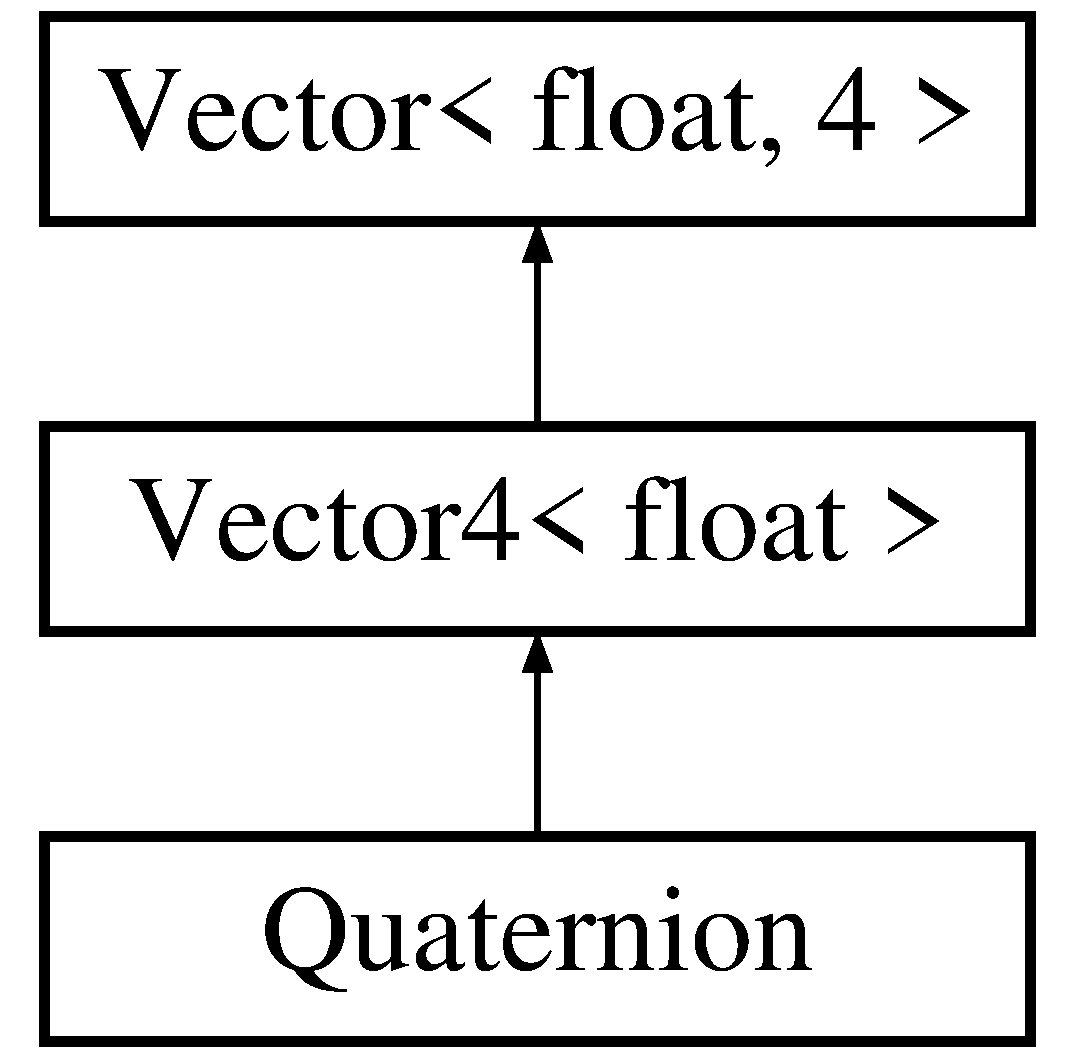
\includegraphics[height=3.000000cm]{class_quaternion}
\end{center}
\end{figure}
\subsection*{Public Member Functions}
\begin{DoxyCompactItemize}
\item 
\hyperlink{class_quaternion_a3206d7879f2446e1e7722d5d443f9a34}{Quaternion} (float x=0.\+0f, float y=0.\+0f, float z=0.\+0f, float w=1.\+0f)
\item 
\hyperlink{class_quaternion_afcc45f2a528b5b22dbd650566924c3a6}{Quaternion} (const \hyperlink{class_vector4}{Vector4}$<$ float $>$ \&r)
\item 
\hyperlink{class_quaternion_a45c7466afad2a6ab7b27d3199332bf26}{Quaternion} (const \hyperlink{class_vector3f}{Vector3f} \&axis, float angle)
\item 
\hyperlink{class_quaternion_abbc3809120e7f0d3ef7e4ac7f1ef45cd}{Quaternion} (const \hyperlink{math3d_8h_a5b7721ab7216c91a40538beaa9e6ee1f}{Matrix4f} \&m)
\item 
\hyperlink{class_quaternion}{Quaternion} \hyperlink{class_quaternion_ad01607c48ca84db58804369317ec2df4}{N\+Lerp} (const \hyperlink{class_quaternion}{Quaternion} \&r, float lerp\+Factor, bool shortest\+Path) const 
\item 
\hyperlink{class_quaternion}{Quaternion} \hyperlink{class_quaternion_a84b8812c677f8c3e6112977e3c763f32}{S\+Lerp} (const \hyperlink{class_quaternion}{Quaternion} \&r, float lerp\+Factor, bool shortest\+Path) const 
\item 
\hyperlink{math3d_8h_a5b7721ab7216c91a40538beaa9e6ee1f}{Matrix4f} \hyperlink{class_quaternion_aa5d6a6752bb54dffe8eba74d4828313e}{To\+Rotation\+Matrix} () const 
\item 
bt\+Quaternion \hyperlink{class_quaternion_a933a2ca26bf9794299bad74a4c6d6841}{Get\+B\+T} () const 
\item 
\hyperlink{class_vector3f}{Vector3f} \hyperlink{class_quaternion_affda2740ce48497e8774640fa7121a78}{Get\+Forward} () const 
\item 
\hyperlink{class_vector3f}{Vector3f} \hyperlink{class_quaternion_a3a3c05d15a7fe1247de0eaff29c6152a}{Get\+Back} () const 
\item 
\hyperlink{class_vector3f}{Vector3f} \hyperlink{class_quaternion_ad46bcac60f877d93dc988f4791d934eb}{Get\+Up} () const 
\item 
\hyperlink{class_vector3f}{Vector3f} \hyperlink{class_quaternion_a98620ca1d2b938e6dfd9277ef6b33af6}{Get\+Down} () const 
\item 
\hyperlink{class_vector3f}{Vector3f} \hyperlink{class_quaternion_a0c62c6ea03f73ac020eda6060533cfc8}{Get\+Right} () const 
\item 
\hyperlink{class_vector3f}{Vector3f} \hyperlink{class_quaternion_af7ba3193650c9c9637e7753b519c29a5}{Get\+Left} () const 
\item 
\hyperlink{class_quaternion}{Quaternion} \hyperlink{class_quaternion_a0ee64800ff331f0a7d2572c86f98b83b}{Conjugate} () const 
\item 
\hyperlink{class_quaternion}{Quaternion} \hyperlink{class_quaternion_ab71aea5a41302f8f82e2db04774da03a}{operator$\ast$} (const \hyperlink{class_quaternion}{Quaternion} \&r) const 
\item 
\hyperlink{class_quaternion}{Quaternion} \hyperlink{class_quaternion_a74472bb4c7261dfb15df158528752201}{operator$\ast$} (const \hyperlink{class_vector3}{Vector3}$<$ float $>$ \&v) const 
\end{DoxyCompactItemize}
\subsection*{Static Public Member Functions}
\begin{DoxyCompactItemize}
\item 
static \hyperlink{class_quaternion}{Quaternion} \hyperlink{class_quaternion_add054c81079e45517b3a275ed60cdc6d}{Get\+F\+T} (const bt\+Quaternion \&bt)
\end{DoxyCompactItemize}


\subsection{Constructor \& Destructor Documentation}
\hypertarget{class_quaternion_a3206d7879f2446e1e7722d5d443f9a34}{}\index{Quaternion@{Quaternion}!Quaternion@{Quaternion}}
\index{Quaternion@{Quaternion}!Quaternion@{Quaternion}}
\subsubsection[{Quaternion(float x=0.\+0f, float y=0.\+0f, float z=0.\+0f, float w=1.\+0f)}]{\setlength{\rightskip}{0pt plus 5cm}Quaternion\+::\+Quaternion (
\begin{DoxyParamCaption}
\item[{float}]{x = {\ttfamily 0.0f}, }
\item[{float}]{y = {\ttfamily 0.0f}, }
\item[{float}]{z = {\ttfamily 0.0f}, }
\item[{float}]{w = {\ttfamily 1.0f}}
\end{DoxyParamCaption}
)\hspace{0.3cm}{\ttfamily [inline]}}\label{class_quaternion_a3206d7879f2446e1e7722d5d443f9a34}
\hypertarget{class_quaternion_afcc45f2a528b5b22dbd650566924c3a6}{}\index{Quaternion@{Quaternion}!Quaternion@{Quaternion}}
\index{Quaternion@{Quaternion}!Quaternion@{Quaternion}}
\subsubsection[{Quaternion(const Vector4$<$ float $>$ \&r)}]{\setlength{\rightskip}{0pt plus 5cm}Quaternion\+::\+Quaternion (
\begin{DoxyParamCaption}
\item[{const {\bf Vector4}$<$ float $>$ \&}]{r}
\end{DoxyParamCaption}
)\hspace{0.3cm}{\ttfamily [inline]}}\label{class_quaternion_afcc45f2a528b5b22dbd650566924c3a6}
\hypertarget{class_quaternion_a45c7466afad2a6ab7b27d3199332bf26}{}\index{Quaternion@{Quaternion}!Quaternion@{Quaternion}}
\index{Quaternion@{Quaternion}!Quaternion@{Quaternion}}
\subsubsection[{Quaternion(const Vector3f \&axis, float angle)}]{\setlength{\rightskip}{0pt plus 5cm}Quaternion\+::\+Quaternion (
\begin{DoxyParamCaption}
\item[{const {\bf Vector3f} \&}]{axis, }
\item[{float}]{angle}
\end{DoxyParamCaption}
)\hspace{0.3cm}{\ttfamily [inline]}}\label{class_quaternion_a45c7466afad2a6ab7b27d3199332bf26}
\hypertarget{class_quaternion_abbc3809120e7f0d3ef7e4ac7f1ef45cd}{}\index{Quaternion@{Quaternion}!Quaternion@{Quaternion}}
\index{Quaternion@{Quaternion}!Quaternion@{Quaternion}}
\subsubsection[{Quaternion(const Matrix4f \&m)}]{\setlength{\rightskip}{0pt plus 5cm}Quaternion\+::\+Quaternion (
\begin{DoxyParamCaption}
\item[{const {\bf Matrix4f} \&}]{m}
\end{DoxyParamCaption}
)\hspace{0.3cm}{\ttfamily [inline]}}\label{class_quaternion_abbc3809120e7f0d3ef7e4ac7f1ef45cd}


\subsection{Member Function Documentation}
\hypertarget{class_quaternion_a0ee64800ff331f0a7d2572c86f98b83b}{}\index{Quaternion@{Quaternion}!Conjugate@{Conjugate}}
\index{Conjugate@{Conjugate}!Quaternion@{Quaternion}}
\subsubsection[{Conjugate() const }]{\setlength{\rightskip}{0pt plus 5cm}{\bf Quaternion} Quaternion\+::\+Conjugate (
\begin{DoxyParamCaption}
{}
\end{DoxyParamCaption}
) const\hspace{0.3cm}{\ttfamily [inline]}}\label{class_quaternion_a0ee64800ff331f0a7d2572c86f98b83b}
\hypertarget{class_quaternion_a3a3c05d15a7fe1247de0eaff29c6152a}{}\index{Quaternion@{Quaternion}!Get\+Back@{Get\+Back}}
\index{Get\+Back@{Get\+Back}!Quaternion@{Quaternion}}
\subsubsection[{Get\+Back() const }]{\setlength{\rightskip}{0pt plus 5cm}{\bf Vector3f} Quaternion\+::\+Get\+Back (
\begin{DoxyParamCaption}
{}
\end{DoxyParamCaption}
) const\hspace{0.3cm}{\ttfamily [inline]}}\label{class_quaternion_a3a3c05d15a7fe1247de0eaff29c6152a}
\hypertarget{class_quaternion_a933a2ca26bf9794299bad74a4c6d6841}{}\index{Quaternion@{Quaternion}!Get\+B\+T@{Get\+B\+T}}
\index{Get\+B\+T@{Get\+B\+T}!Quaternion@{Quaternion}}
\subsubsection[{Get\+B\+T() const }]{\setlength{\rightskip}{0pt plus 5cm}bt\+Quaternion Quaternion\+::\+Get\+B\+T (
\begin{DoxyParamCaption}
{}
\end{DoxyParamCaption}
) const\hspace{0.3cm}{\ttfamily [inline]}}\label{class_quaternion_a933a2ca26bf9794299bad74a4c6d6841}
\hypertarget{class_quaternion_a98620ca1d2b938e6dfd9277ef6b33af6}{}\index{Quaternion@{Quaternion}!Get\+Down@{Get\+Down}}
\index{Get\+Down@{Get\+Down}!Quaternion@{Quaternion}}
\subsubsection[{Get\+Down() const }]{\setlength{\rightskip}{0pt plus 5cm}{\bf Vector3f} Quaternion\+::\+Get\+Down (
\begin{DoxyParamCaption}
{}
\end{DoxyParamCaption}
) const\hspace{0.3cm}{\ttfamily [inline]}}\label{class_quaternion_a98620ca1d2b938e6dfd9277ef6b33af6}
\hypertarget{class_quaternion_affda2740ce48497e8774640fa7121a78}{}\index{Quaternion@{Quaternion}!Get\+Forward@{Get\+Forward}}
\index{Get\+Forward@{Get\+Forward}!Quaternion@{Quaternion}}
\subsubsection[{Get\+Forward() const }]{\setlength{\rightskip}{0pt plus 5cm}{\bf Vector3f} Quaternion\+::\+Get\+Forward (
\begin{DoxyParamCaption}
{}
\end{DoxyParamCaption}
) const\hspace{0.3cm}{\ttfamily [inline]}}\label{class_quaternion_affda2740ce48497e8774640fa7121a78}
\hypertarget{class_quaternion_add054c81079e45517b3a275ed60cdc6d}{}\index{Quaternion@{Quaternion}!Get\+F\+T@{Get\+F\+T}}
\index{Get\+F\+T@{Get\+F\+T}!Quaternion@{Quaternion}}
\subsubsection[{Get\+F\+T(const bt\+Quaternion \&bt)}]{\setlength{\rightskip}{0pt plus 5cm}static {\bf Quaternion} Quaternion\+::\+Get\+F\+T (
\begin{DoxyParamCaption}
\item[{const bt\+Quaternion \&}]{bt}
\end{DoxyParamCaption}
)\hspace{0.3cm}{\ttfamily [inline]}, {\ttfamily [static]}}\label{class_quaternion_add054c81079e45517b3a275ed60cdc6d}
\hypertarget{class_quaternion_af7ba3193650c9c9637e7753b519c29a5}{}\index{Quaternion@{Quaternion}!Get\+Left@{Get\+Left}}
\index{Get\+Left@{Get\+Left}!Quaternion@{Quaternion}}
\subsubsection[{Get\+Left() const }]{\setlength{\rightskip}{0pt plus 5cm}{\bf Vector3f} Quaternion\+::\+Get\+Left (
\begin{DoxyParamCaption}
{}
\end{DoxyParamCaption}
) const\hspace{0.3cm}{\ttfamily [inline]}}\label{class_quaternion_af7ba3193650c9c9637e7753b519c29a5}
\hypertarget{class_quaternion_a0c62c6ea03f73ac020eda6060533cfc8}{}\index{Quaternion@{Quaternion}!Get\+Right@{Get\+Right}}
\index{Get\+Right@{Get\+Right}!Quaternion@{Quaternion}}
\subsubsection[{Get\+Right() const }]{\setlength{\rightskip}{0pt plus 5cm}{\bf Vector3f} Quaternion\+::\+Get\+Right (
\begin{DoxyParamCaption}
{}
\end{DoxyParamCaption}
) const\hspace{0.3cm}{\ttfamily [inline]}}\label{class_quaternion_a0c62c6ea03f73ac020eda6060533cfc8}
\hypertarget{class_quaternion_ad46bcac60f877d93dc988f4791d934eb}{}\index{Quaternion@{Quaternion}!Get\+Up@{Get\+Up}}
\index{Get\+Up@{Get\+Up}!Quaternion@{Quaternion}}
\subsubsection[{Get\+Up() const }]{\setlength{\rightskip}{0pt plus 5cm}{\bf Vector3f} Quaternion\+::\+Get\+Up (
\begin{DoxyParamCaption}
{}
\end{DoxyParamCaption}
) const\hspace{0.3cm}{\ttfamily [inline]}}\label{class_quaternion_ad46bcac60f877d93dc988f4791d934eb}
\hypertarget{class_quaternion_ad01607c48ca84db58804369317ec2df4}{}\index{Quaternion@{Quaternion}!N\+Lerp@{N\+Lerp}}
\index{N\+Lerp@{N\+Lerp}!Quaternion@{Quaternion}}
\subsubsection[{N\+Lerp(const Quaternion \&r, float lerp\+Factor, bool shortest\+Path) const }]{\setlength{\rightskip}{0pt plus 5cm}{\bf Quaternion} Quaternion\+::\+N\+Lerp (
\begin{DoxyParamCaption}
\item[{const {\bf Quaternion} \&}]{r, }
\item[{float}]{lerp\+Factor, }
\item[{bool}]{shortest\+Path}
\end{DoxyParamCaption}
) const\hspace{0.3cm}{\ttfamily [inline]}}\label{class_quaternion_ad01607c48ca84db58804369317ec2df4}
\hypertarget{class_quaternion_ab71aea5a41302f8f82e2db04774da03a}{}\index{Quaternion@{Quaternion}!operator$\ast$@{operator$\ast$}}
\index{operator$\ast$@{operator$\ast$}!Quaternion@{Quaternion}}
\subsubsection[{operator$\ast$(const Quaternion \&r) const }]{\setlength{\rightskip}{0pt plus 5cm}{\bf Quaternion} Quaternion\+::operator$\ast$ (
\begin{DoxyParamCaption}
\item[{const {\bf Quaternion} \&}]{r}
\end{DoxyParamCaption}
) const\hspace{0.3cm}{\ttfamily [inline]}}\label{class_quaternion_ab71aea5a41302f8f82e2db04774da03a}
\hypertarget{class_quaternion_a74472bb4c7261dfb15df158528752201}{}\index{Quaternion@{Quaternion}!operator$\ast$@{operator$\ast$}}
\index{operator$\ast$@{operator$\ast$}!Quaternion@{Quaternion}}
\subsubsection[{operator$\ast$(const Vector3$<$ float $>$ \&v) const }]{\setlength{\rightskip}{0pt plus 5cm}{\bf Quaternion} Quaternion\+::operator$\ast$ (
\begin{DoxyParamCaption}
\item[{const {\bf Vector3}$<$ float $>$ \&}]{v}
\end{DoxyParamCaption}
) const\hspace{0.3cm}{\ttfamily [inline]}}\label{class_quaternion_a74472bb4c7261dfb15df158528752201}
\hypertarget{class_quaternion_a84b8812c677f8c3e6112977e3c763f32}{}\index{Quaternion@{Quaternion}!S\+Lerp@{S\+Lerp}}
\index{S\+Lerp@{S\+Lerp}!Quaternion@{Quaternion}}
\subsubsection[{S\+Lerp(const Quaternion \&r, float lerp\+Factor, bool shortest\+Path) const }]{\setlength{\rightskip}{0pt plus 5cm}{\bf Quaternion} Quaternion\+::\+S\+Lerp (
\begin{DoxyParamCaption}
\item[{const {\bf Quaternion} \&}]{r, }
\item[{float}]{lerp\+Factor, }
\item[{bool}]{shortest\+Path}
\end{DoxyParamCaption}
) const\hspace{0.3cm}{\ttfamily [inline]}}\label{class_quaternion_a84b8812c677f8c3e6112977e3c763f32}
\hypertarget{class_quaternion_aa5d6a6752bb54dffe8eba74d4828313e}{}\index{Quaternion@{Quaternion}!To\+Rotation\+Matrix@{To\+Rotation\+Matrix}}
\index{To\+Rotation\+Matrix@{To\+Rotation\+Matrix}!Quaternion@{Quaternion}}
\subsubsection[{To\+Rotation\+Matrix() const }]{\setlength{\rightskip}{0pt plus 5cm}{\bf Matrix4f} Quaternion\+::\+To\+Rotation\+Matrix (
\begin{DoxyParamCaption}
{}
\end{DoxyParamCaption}
) const\hspace{0.3cm}{\ttfamily [inline]}}\label{class_quaternion_aa5d6a6752bb54dffe8eba74d4828313e}


The documentation for this class was generated from the following file\+:\begin{DoxyCompactItemize}
\item 
F\+:/\+Fusion3\+D\+\_\+work/src/core/\hyperlink{math3d_8h}{math3d.\+h}\end{DoxyCompactItemize}

\hypertarget{class_reference_counter}{}\section{Reference\+Counter Class Reference}
\label{class_reference_counter}\index{Reference\+Counter@{Reference\+Counter}}


{\ttfamily \#include $<$reference\+Counter.\+h$>$}

Inheritance diagram for Reference\+Counter\+:\begin{figure}[H]
\begin{center}
\leavevmode
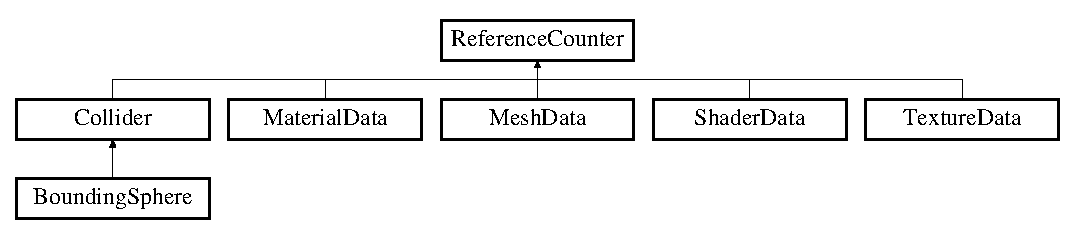
\includegraphics[height=2.709677cm]{class_reference_counter}
\end{center}
\end{figure}
\subsection*{Public Member Functions}
\begin{DoxyCompactItemize}
\item 
\hyperlink{class_reference_counter_a6389ca70c8a41c4d2f1a4e72d42e9780}{Reference\+Counter} ()
\item 
int \hyperlink{class_reference_counter_a806c028262198a7bc28cdad238680863}{Get\+Reference\+Count} ()
\item 
void \hyperlink{class_reference_counter_a2675ccf5f6400a629040da7b4ae4a701}{Add\+Reference} ()
\item 
bool \hyperlink{class_reference_counter_a6b0ff351858d3ff37dc8946a8c148885}{Remove\+Reference} ()
\end{DoxyCompactItemize}


\subsection{Constructor \& Destructor Documentation}
\hypertarget{class_reference_counter_a6389ca70c8a41c4d2f1a4e72d42e9780}{}\index{Reference\+Counter@{Reference\+Counter}!Reference\+Counter@{Reference\+Counter}}
\index{Reference\+Counter@{Reference\+Counter}!Reference\+Counter@{Reference\+Counter}}
\subsubsection[{Reference\+Counter()}]{\setlength{\rightskip}{0pt plus 5cm}Reference\+Counter\+::\+Reference\+Counter (
\begin{DoxyParamCaption}
{}
\end{DoxyParamCaption}
)\hspace{0.3cm}{\ttfamily [inline]}}\label{class_reference_counter_a6389ca70c8a41c4d2f1a4e72d42e9780}


\subsection{Member Function Documentation}
\hypertarget{class_reference_counter_a2675ccf5f6400a629040da7b4ae4a701}{}\index{Reference\+Counter@{Reference\+Counter}!Add\+Reference@{Add\+Reference}}
\index{Add\+Reference@{Add\+Reference}!Reference\+Counter@{Reference\+Counter}}
\subsubsection[{Add\+Reference()}]{\setlength{\rightskip}{0pt plus 5cm}void Reference\+Counter\+::\+Add\+Reference (
\begin{DoxyParamCaption}
{}
\end{DoxyParamCaption}
)\hspace{0.3cm}{\ttfamily [inline]}}\label{class_reference_counter_a2675ccf5f6400a629040da7b4ae4a701}
\hypertarget{class_reference_counter_a806c028262198a7bc28cdad238680863}{}\index{Reference\+Counter@{Reference\+Counter}!Get\+Reference\+Count@{Get\+Reference\+Count}}
\index{Get\+Reference\+Count@{Get\+Reference\+Count}!Reference\+Counter@{Reference\+Counter}}
\subsubsection[{Get\+Reference\+Count()}]{\setlength{\rightskip}{0pt plus 5cm}int Reference\+Counter\+::\+Get\+Reference\+Count (
\begin{DoxyParamCaption}
{}
\end{DoxyParamCaption}
)\hspace{0.3cm}{\ttfamily [inline]}}\label{class_reference_counter_a806c028262198a7bc28cdad238680863}
\hypertarget{class_reference_counter_a6b0ff351858d3ff37dc8946a8c148885}{}\index{Reference\+Counter@{Reference\+Counter}!Remove\+Reference@{Remove\+Reference}}
\index{Remove\+Reference@{Remove\+Reference}!Reference\+Counter@{Reference\+Counter}}
\subsubsection[{Remove\+Reference()}]{\setlength{\rightskip}{0pt plus 5cm}bool Reference\+Counter\+::\+Remove\+Reference (
\begin{DoxyParamCaption}
{}
\end{DoxyParamCaption}
)\hspace{0.3cm}{\ttfamily [inline]}}\label{class_reference_counter_a6b0ff351858d3ff37dc8946a8c148885}


The documentation for this class was generated from the following file\+:\begin{DoxyCompactItemize}
\item 
F\+:/\+Fusion3\+D\+\_\+work/src/core/\hyperlink{reference_counter_8h}{reference\+Counter.\+h}\end{DoxyCompactItemize}

\hypertarget{class_rendering_engine}{}\section{Rendering\+Engine Class Reference}
\label{class_rendering_engine}\index{Rendering\+Engine@{Rendering\+Engine}}


{\ttfamily \#include $<$rendering\+Engine.\+h$>$}

Inheritance diagram for Rendering\+Engine\+:\begin{figure}[H]
\begin{center}
\leavevmode
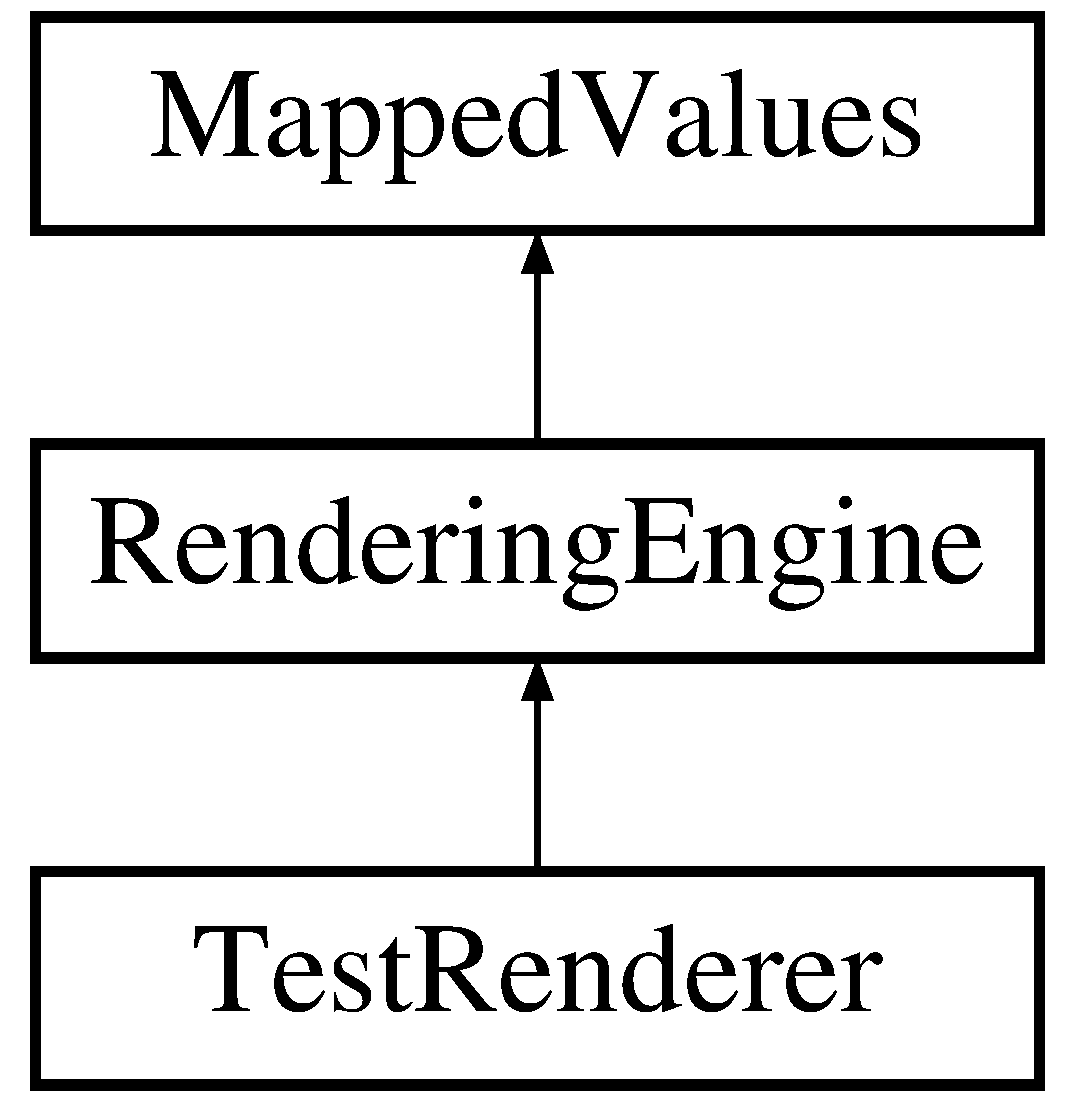
\includegraphics[height=3.000000cm]{class_rendering_engine}
\end{center}
\end{figure}
\subsection*{Public Member Functions}
\begin{DoxyCompactItemize}
\item 
\hyperlink{class_rendering_engine_a0e21c88e8062f84c4ac72eaeee7589b7}{Rendering\+Engine} (\hyperlink{class_window}{Window} $\ast$window)
\item 
virtual \hyperlink{class_rendering_engine_a88d03066dde2aff01969125ec4cad81d}{$\sim$\+Rendering\+Engine} ()
\item 
virtual void \hyperlink{class_rendering_engine_a38ac5d7f0ed4b4933c232ca00a3adde5}{Render} (const \hyperlink{class_entity}{Entity} \&object)
\item 
void \hyperlink{class_rendering_engine_abdb38492f5b6ce91faf67be45a4f8398}{Add\+Light} (\hyperlink{lighting_8h_a5796f1b946d6b585e607c4d0df3a0d8f}{Base\+Light} $\ast$light)
\item 
void \hyperlink{class_rendering_engine_ab4129c1f16613cf99a42af5e9a25a94d}{Set\+Main\+Camera} (const \hyperlink{class_camera}{Camera} \&camera)
\item 
const \hyperlink{class_camera}{Camera} $\ast$ \hyperlink{class_rendering_engine_a82df5730a81c8dcc7396db4faea0475b}{Get\+Main\+Camera} ()
\item 
virtual void \hyperlink{class_rendering_engine_ad585884dd7d40bc347b729985edd214e}{Update\+Uniform\+Struct} (const \hyperlink{class_transform}{Transform} \&transform, const \hyperlink{class_material}{Material} \&material, const \hyperlink{class_shader}{Shader} \&shader, const std\+::string \&uniform\+Name, const std\+::string \&uniform\+Type) const 
\item 
double \hyperlink{class_rendering_engine_a9207fd39818ffb3522e5450cd5303b15}{Display\+Render\+Time} (double dividend)
\item 
double \hyperlink{class_rendering_engine_a552848b25ff08e2c6961570504291eaa}{Display\+Window\+Sync\+Time} (double dividend)
\item 
void \hyperlink{class_rendering_engine_ac7087d3f4ace79e7c1671549959c3bcd}{Set\+Shader} (const std\+::string \&file\+Name)
\item 
void \hyperlink{class_rendering_engine_ab00fce20ca35e752481114e05ef1eab1}{Set\+Full\+Bright} (bool state)
\item 
const \hyperlink{lighting_8h_a5796f1b946d6b585e607c4d0df3a0d8f}{Base\+Light} \& \hyperlink{class_rendering_engine_a8fcd0abd0d6d85938daab3e2a53586c3}{Get\+Active\+Light} () const 
\item 
unsigned int \hyperlink{class_rendering_engine_a61b5cf1c219f9a2514e9c44818dd25a8}{Get\+Sampler\+Slot} (const std\+::string \&sampler\+Name) const 
\item 
const \hyperlink{math3d_8h_a5b7721ab7216c91a40538beaa9e6ee1f}{Matrix4f} \& \hyperlink{class_rendering_engine_a0765f39bf7970cb6cb9f2de446f86671}{Get\+Light\+Matrix} () const 
\end{DoxyCompactItemize}
\subsection*{Protected Member Functions}
\begin{DoxyCompactItemize}
\item 
void \hyperlink{class_rendering_engine_a5b6784d215f8ed44ac5fabaa9457811c}{Set\+Sampler\+Slot} (const std\+::string \&name, unsigned int value)
\end{DoxyCompactItemize}


\subsection{Constructor \& Destructor Documentation}
\hypertarget{class_rendering_engine_a0e21c88e8062f84c4ac72eaeee7589b7}{}\index{Rendering\+Engine@{Rendering\+Engine}!Rendering\+Engine@{Rendering\+Engine}}
\index{Rendering\+Engine@{Rendering\+Engine}!Rendering\+Engine@{Rendering\+Engine}}
\subsubsection[{Rendering\+Engine(\+Window $\ast$window)}]{\setlength{\rightskip}{0pt plus 5cm}Rendering\+Engine\+::\+Rendering\+Engine (
\begin{DoxyParamCaption}
\item[{{\bf Window} $\ast$}]{window}
\end{DoxyParamCaption}
)}\label{class_rendering_engine_a0e21c88e8062f84c4ac72eaeee7589b7}
\hypertarget{class_rendering_engine_a88d03066dde2aff01969125ec4cad81d}{}\index{Rendering\+Engine@{Rendering\+Engine}!````~Rendering\+Engine@{$\sim$\+Rendering\+Engine}}
\index{````~Rendering\+Engine@{$\sim$\+Rendering\+Engine}!Rendering\+Engine@{Rendering\+Engine}}
\subsubsection[{$\sim$\+Rendering\+Engine()}]{\setlength{\rightskip}{0pt plus 5cm}virtual Rendering\+Engine\+::$\sim$\+Rendering\+Engine (
\begin{DoxyParamCaption}
{}
\end{DoxyParamCaption}
)\hspace{0.3cm}{\ttfamily [inline]}, {\ttfamily [virtual]}}\label{class_rendering_engine_a88d03066dde2aff01969125ec4cad81d}


\subsection{Member Function Documentation}
\hypertarget{class_rendering_engine_abdb38492f5b6ce91faf67be45a4f8398}{}\index{Rendering\+Engine@{Rendering\+Engine}!Add\+Light@{Add\+Light}}
\index{Add\+Light@{Add\+Light}!Rendering\+Engine@{Rendering\+Engine}}
\subsubsection[{Add\+Light(\+Base\+Light $\ast$light)}]{\setlength{\rightskip}{0pt plus 5cm}void Rendering\+Engine\+::\+Add\+Light (
\begin{DoxyParamCaption}
\item[{{\bf Base\+Light} $\ast$}]{light}
\end{DoxyParamCaption}
)\hspace{0.3cm}{\ttfamily [inline]}}\label{class_rendering_engine_abdb38492f5b6ce91faf67be45a4f8398}
\hypertarget{class_rendering_engine_a9207fd39818ffb3522e5450cd5303b15}{}\index{Rendering\+Engine@{Rendering\+Engine}!Display\+Render\+Time@{Display\+Render\+Time}}
\index{Display\+Render\+Time@{Display\+Render\+Time}!Rendering\+Engine@{Rendering\+Engine}}
\subsubsection[{Display\+Render\+Time(double dividend)}]{\setlength{\rightskip}{0pt plus 5cm}double Rendering\+Engine\+::\+Display\+Render\+Time (
\begin{DoxyParamCaption}
\item[{double}]{dividend}
\end{DoxyParamCaption}
)\hspace{0.3cm}{\ttfamily [inline]}}\label{class_rendering_engine_a9207fd39818ffb3522e5450cd5303b15}
\hypertarget{class_rendering_engine_a552848b25ff08e2c6961570504291eaa}{}\index{Rendering\+Engine@{Rendering\+Engine}!Display\+Window\+Sync\+Time@{Display\+Window\+Sync\+Time}}
\index{Display\+Window\+Sync\+Time@{Display\+Window\+Sync\+Time}!Rendering\+Engine@{Rendering\+Engine}}
\subsubsection[{Display\+Window\+Sync\+Time(double dividend)}]{\setlength{\rightskip}{0pt plus 5cm}double Rendering\+Engine\+::\+Display\+Window\+Sync\+Time (
\begin{DoxyParamCaption}
\item[{double}]{dividend}
\end{DoxyParamCaption}
)\hspace{0.3cm}{\ttfamily [inline]}}\label{class_rendering_engine_a552848b25ff08e2c6961570504291eaa}
\hypertarget{class_rendering_engine_a8fcd0abd0d6d85938daab3e2a53586c3}{}\index{Rendering\+Engine@{Rendering\+Engine}!Get\+Active\+Light@{Get\+Active\+Light}}
\index{Get\+Active\+Light@{Get\+Active\+Light}!Rendering\+Engine@{Rendering\+Engine}}
\subsubsection[{Get\+Active\+Light() const }]{\setlength{\rightskip}{0pt plus 5cm}const {\bf Base\+Light}\& Rendering\+Engine\+::\+Get\+Active\+Light (
\begin{DoxyParamCaption}
{}
\end{DoxyParamCaption}
) const\hspace{0.3cm}{\ttfamily [inline]}}\label{class_rendering_engine_a8fcd0abd0d6d85938daab3e2a53586c3}
\hypertarget{class_rendering_engine_a0765f39bf7970cb6cb9f2de446f86671}{}\index{Rendering\+Engine@{Rendering\+Engine}!Get\+Light\+Matrix@{Get\+Light\+Matrix}}
\index{Get\+Light\+Matrix@{Get\+Light\+Matrix}!Rendering\+Engine@{Rendering\+Engine}}
\subsubsection[{Get\+Light\+Matrix() const }]{\setlength{\rightskip}{0pt plus 5cm}const {\bf Matrix4f}\& Rendering\+Engine\+::\+Get\+Light\+Matrix (
\begin{DoxyParamCaption}
{}
\end{DoxyParamCaption}
) const\hspace{0.3cm}{\ttfamily [inline]}}\label{class_rendering_engine_a0765f39bf7970cb6cb9f2de446f86671}
\hypertarget{class_rendering_engine_a82df5730a81c8dcc7396db4faea0475b}{}\index{Rendering\+Engine@{Rendering\+Engine}!Get\+Main\+Camera@{Get\+Main\+Camera}}
\index{Get\+Main\+Camera@{Get\+Main\+Camera}!Rendering\+Engine@{Rendering\+Engine}}
\subsubsection[{Get\+Main\+Camera()}]{\setlength{\rightskip}{0pt plus 5cm}const {\bf Camera}$\ast$ Rendering\+Engine\+::\+Get\+Main\+Camera (
\begin{DoxyParamCaption}
{}
\end{DoxyParamCaption}
)\hspace{0.3cm}{\ttfamily [inline]}}\label{class_rendering_engine_a82df5730a81c8dcc7396db4faea0475b}
\hypertarget{class_rendering_engine_a61b5cf1c219f9a2514e9c44818dd25a8}{}\index{Rendering\+Engine@{Rendering\+Engine}!Get\+Sampler\+Slot@{Get\+Sampler\+Slot}}
\index{Get\+Sampler\+Slot@{Get\+Sampler\+Slot}!Rendering\+Engine@{Rendering\+Engine}}
\subsubsection[{Get\+Sampler\+Slot(const std\+::string \&sampler\+Name) const }]{\setlength{\rightskip}{0pt plus 5cm}unsigned int Rendering\+Engine\+::\+Get\+Sampler\+Slot (
\begin{DoxyParamCaption}
\item[{const std\+::string \&}]{sampler\+Name}
\end{DoxyParamCaption}
) const\hspace{0.3cm}{\ttfamily [inline]}}\label{class_rendering_engine_a61b5cf1c219f9a2514e9c44818dd25a8}
\hypertarget{class_rendering_engine_a38ac5d7f0ed4b4933c232ca00a3adde5}{}\index{Rendering\+Engine@{Rendering\+Engine}!Render@{Render}}
\index{Render@{Render}!Rendering\+Engine@{Rendering\+Engine}}
\subsubsection[{Render(const Entity \&object)}]{\setlength{\rightskip}{0pt plus 5cm}void Rendering\+Engine\+::\+Render (
\begin{DoxyParamCaption}
\item[{const {\bf Entity} \&}]{object}
\end{DoxyParamCaption}
)\hspace{0.3cm}{\ttfamily [virtual]}}\label{class_rendering_engine_a38ac5d7f0ed4b4933c232ca00a3adde5}


Reimplemented in \hyperlink{class_test_renderer_abe86af4ad1aa4d3d68a08468ebab8f9e}{Test\+Renderer}.

\hypertarget{class_rendering_engine_ab00fce20ca35e752481114e05ef1eab1}{}\index{Rendering\+Engine@{Rendering\+Engine}!Set\+Full\+Bright@{Set\+Full\+Bright}}
\index{Set\+Full\+Bright@{Set\+Full\+Bright}!Rendering\+Engine@{Rendering\+Engine}}
\subsubsection[{Set\+Full\+Bright(bool state)}]{\setlength{\rightskip}{0pt plus 5cm}void Rendering\+Engine\+::\+Set\+Full\+Bright (
\begin{DoxyParamCaption}
\item[{bool}]{state}
\end{DoxyParamCaption}
)\hspace{0.3cm}{\ttfamily [inline]}}\label{class_rendering_engine_ab00fce20ca35e752481114e05ef1eab1}
\hypertarget{class_rendering_engine_ab4129c1f16613cf99a42af5e9a25a94d}{}\index{Rendering\+Engine@{Rendering\+Engine}!Set\+Main\+Camera@{Set\+Main\+Camera}}
\index{Set\+Main\+Camera@{Set\+Main\+Camera}!Rendering\+Engine@{Rendering\+Engine}}
\subsubsection[{Set\+Main\+Camera(const Camera \&camera)}]{\setlength{\rightskip}{0pt plus 5cm}void Rendering\+Engine\+::\+Set\+Main\+Camera (
\begin{DoxyParamCaption}
\item[{const {\bf Camera} \&}]{camera}
\end{DoxyParamCaption}
)\hspace{0.3cm}{\ttfamily [inline]}}\label{class_rendering_engine_ab4129c1f16613cf99a42af5e9a25a94d}
\hypertarget{class_rendering_engine_a5b6784d215f8ed44ac5fabaa9457811c}{}\index{Rendering\+Engine@{Rendering\+Engine}!Set\+Sampler\+Slot@{Set\+Sampler\+Slot}}
\index{Set\+Sampler\+Slot@{Set\+Sampler\+Slot}!Rendering\+Engine@{Rendering\+Engine}}
\subsubsection[{Set\+Sampler\+Slot(const std\+::string \&name, unsigned int value)}]{\setlength{\rightskip}{0pt plus 5cm}void Rendering\+Engine\+::\+Set\+Sampler\+Slot (
\begin{DoxyParamCaption}
\item[{const std\+::string \&}]{name, }
\item[{unsigned int}]{value}
\end{DoxyParamCaption}
)\hspace{0.3cm}{\ttfamily [inline]}, {\ttfamily [protected]}}\label{class_rendering_engine_a5b6784d215f8ed44ac5fabaa9457811c}
\hypertarget{class_rendering_engine_ac7087d3f4ace79e7c1671549959c3bcd}{}\index{Rendering\+Engine@{Rendering\+Engine}!Set\+Shader@{Set\+Shader}}
\index{Set\+Shader@{Set\+Shader}!Rendering\+Engine@{Rendering\+Engine}}
\subsubsection[{Set\+Shader(const std\+::string \&file\+Name)}]{\setlength{\rightskip}{0pt plus 5cm}void Rendering\+Engine\+::\+Set\+Shader (
\begin{DoxyParamCaption}
\item[{const std\+::string \&}]{file\+Name}
\end{DoxyParamCaption}
)\hspace{0.3cm}{\ttfamily [inline]}}\label{class_rendering_engine_ac7087d3f4ace79e7c1671549959c3bcd}
\hypertarget{class_rendering_engine_ad585884dd7d40bc347b729985edd214e}{}\index{Rendering\+Engine@{Rendering\+Engine}!Update\+Uniform\+Struct@{Update\+Uniform\+Struct}}
\index{Update\+Uniform\+Struct@{Update\+Uniform\+Struct}!Rendering\+Engine@{Rendering\+Engine}}
\subsubsection[{Update\+Uniform\+Struct(const Transform \&transform, const Material \&material, const Shader \&shader, const std\+::string \&uniform\+Name, const std\+::string \&uniform\+Type) const }]{\setlength{\rightskip}{0pt plus 5cm}virtual void Rendering\+Engine\+::\+Update\+Uniform\+Struct (
\begin{DoxyParamCaption}
\item[{const {\bf Transform} \&}]{transform, }
\item[{const {\bf Material} \&}]{material, }
\item[{const {\bf Shader} \&}]{shader, }
\item[{const std\+::string \&}]{uniform\+Name, }
\item[{const std\+::string \&}]{uniform\+Type}
\end{DoxyParamCaption}
) const\hspace{0.3cm}{\ttfamily [inline]}, {\ttfamily [virtual]}}\label{class_rendering_engine_ad585884dd7d40bc347b729985edd214e}


The documentation for this class was generated from the following files\+:\begin{DoxyCompactItemize}
\item 
F\+:/\+Fusion3\+D\+\_\+work/src/rendering/\hyperlink{rendering_engine_8h}{rendering\+Engine.\+h}\item 
F\+:/\+Fusion3\+D\+\_\+work/src/rendering/\hyperlink{rendering_engine_8cpp}{rendering\+Engine.\+cpp}\end{DoxyCompactItemize}

\hypertarget{class_shader}{}\section{Shader Class Reference}
\label{class_shader}\index{Shader@{Shader}}


{\ttfamily \#include $<$shader.\+h$>$}

\subsection*{Public Member Functions}
\begin{DoxyCompactItemize}
\item 
\hyperlink{class_shader_aa77ff87040a96fc59c281a4db18779ac}{Shader} (const std\+::string \&file\+Name=\char`\"{}basic\+Shader\char`\"{})
\item 
\hyperlink{class_shader_adab8e450ec1f4509c1bdf147e47a871c}{Shader} (const \hyperlink{class_shader}{Shader} \&other)
\item 
virtual \hyperlink{class_shader_aff01df87e8a102f270b5b135a295e59d}{$\sim$\+Shader} ()
\item 
void \hyperlink{class_shader_a80b52feb71b870447cd0f2a20ca68400}{Bind} () const 
\item 
virtual void \hyperlink{class_shader_a0a6b91d25a352e72624a26cb05f21962}{Update\+Uniforms} (const \hyperlink{class_transform}{Transform} \&transform, const \hyperlink{class_material}{Material} \&material, const \hyperlink{class_rendering_engine}{Rendering\+Engine} \&rendering\+Engine, const \hyperlink{class_camera}{Camera} \&camera) const 
\item 
void \hyperlink{class_shader_a1215713a36b12d48c1c94b56c889c269}{Set\+Uniformi} (const std\+::string \&uniform\+Name, int value) const 
\item 
void \hyperlink{class_shader_aad923978e650300bfe1f82e6ec132fc3}{Set\+Uniformf} (const std\+::string \&uniform\+Name, float value) const 
\item 
void \hyperlink{class_shader_a7633ff5ad50e12c6e8a86d4914d73335}{Set\+Uniform\+Matrix4f} (const std\+::string \&uniform\+Name, const \hyperlink{math3d_8h_a5b7721ab7216c91a40538beaa9e6ee1f}{Matrix4f} \&value) const 
\item 
void \hyperlink{class_shader_aab04027c10b4d5abe5a0095713471c37}{Set\+Uniform\+Vector3f} (const std\+::string \&uniform\+Name, const \hyperlink{class_vector3f}{Vector3f} \&value) const 
\item 
const std\+::string \& \hyperlink{class_shader_a809d60fe373e488a764dc80ac8158330}{Get\+Name} () const 
\end{DoxyCompactItemize}


\subsection{Constructor \& Destructor Documentation}
\hypertarget{class_shader_aa77ff87040a96fc59c281a4db18779ac}{}\index{Shader@{Shader}!Shader@{Shader}}
\index{Shader@{Shader}!Shader@{Shader}}
\subsubsection[{Shader(const std\+::string \&file\+Name=""basic\+Shader"")}]{\setlength{\rightskip}{0pt plus 5cm}Shader\+::\+Shader (
\begin{DoxyParamCaption}
\item[{const std\+::string \&}]{file\+Name = {\ttfamily \char`\"{}basicShader\char`\"{}}}
\end{DoxyParamCaption}
)}\label{class_shader_aa77ff87040a96fc59c281a4db18779ac}
\hypertarget{class_shader_adab8e450ec1f4509c1bdf147e47a871c}{}\index{Shader@{Shader}!Shader@{Shader}}
\index{Shader@{Shader}!Shader@{Shader}}
\subsubsection[{Shader(const Shader \&other)}]{\setlength{\rightskip}{0pt plus 5cm}Shader\+::\+Shader (
\begin{DoxyParamCaption}
\item[{const {\bf Shader} \&}]{other}
\end{DoxyParamCaption}
)}\label{class_shader_adab8e450ec1f4509c1bdf147e47a871c}
\hypertarget{class_shader_aff01df87e8a102f270b5b135a295e59d}{}\index{Shader@{Shader}!````~Shader@{$\sim$\+Shader}}
\index{````~Shader@{$\sim$\+Shader}!Shader@{Shader}}
\subsubsection[{$\sim$\+Shader()}]{\setlength{\rightskip}{0pt plus 5cm}Shader\+::$\sim$\+Shader (
\begin{DoxyParamCaption}
{}
\end{DoxyParamCaption}
)\hspace{0.3cm}{\ttfamily [virtual]}}\label{class_shader_aff01df87e8a102f270b5b135a295e59d}


\subsection{Member Function Documentation}
\hypertarget{class_shader_a80b52feb71b870447cd0f2a20ca68400}{}\index{Shader@{Shader}!Bind@{Bind}}
\index{Bind@{Bind}!Shader@{Shader}}
\subsubsection[{Bind() const }]{\setlength{\rightskip}{0pt plus 5cm}void Shader\+::\+Bind (
\begin{DoxyParamCaption}
{}
\end{DoxyParamCaption}
) const}\label{class_shader_a80b52feb71b870447cd0f2a20ca68400}
\hypertarget{class_shader_a809d60fe373e488a764dc80ac8158330}{}\index{Shader@{Shader}!Get\+Name@{Get\+Name}}
\index{Get\+Name@{Get\+Name}!Shader@{Shader}}
\subsubsection[{Get\+Name() const }]{\setlength{\rightskip}{0pt plus 5cm}const std\+::string\& Shader\+::\+Get\+Name (
\begin{DoxyParamCaption}
{}
\end{DoxyParamCaption}
) const\hspace{0.3cm}{\ttfamily [inline]}}\label{class_shader_a809d60fe373e488a764dc80ac8158330}
\hypertarget{class_shader_aad923978e650300bfe1f82e6ec132fc3}{}\index{Shader@{Shader}!Set\+Uniformf@{Set\+Uniformf}}
\index{Set\+Uniformf@{Set\+Uniformf}!Shader@{Shader}}
\subsubsection[{Set\+Uniformf(const std\+::string \&uniform\+Name, float value) const }]{\setlength{\rightskip}{0pt plus 5cm}void Shader\+::\+Set\+Uniformf (
\begin{DoxyParamCaption}
\item[{const std\+::string \&}]{uniform\+Name, }
\item[{float}]{value}
\end{DoxyParamCaption}
) const}\label{class_shader_aad923978e650300bfe1f82e6ec132fc3}
\hypertarget{class_shader_a1215713a36b12d48c1c94b56c889c269}{}\index{Shader@{Shader}!Set\+Uniformi@{Set\+Uniformi}}
\index{Set\+Uniformi@{Set\+Uniformi}!Shader@{Shader}}
\subsubsection[{Set\+Uniformi(const std\+::string \&uniform\+Name, int value) const }]{\setlength{\rightskip}{0pt plus 5cm}void Shader\+::\+Set\+Uniformi (
\begin{DoxyParamCaption}
\item[{const std\+::string \&}]{uniform\+Name, }
\item[{int}]{value}
\end{DoxyParamCaption}
) const}\label{class_shader_a1215713a36b12d48c1c94b56c889c269}
\hypertarget{class_shader_a7633ff5ad50e12c6e8a86d4914d73335}{}\index{Shader@{Shader}!Set\+Uniform\+Matrix4f@{Set\+Uniform\+Matrix4f}}
\index{Set\+Uniform\+Matrix4f@{Set\+Uniform\+Matrix4f}!Shader@{Shader}}
\subsubsection[{Set\+Uniform\+Matrix4f(const std\+::string \&uniform\+Name, const Matrix4f \&value) const }]{\setlength{\rightskip}{0pt plus 5cm}void Shader\+::\+Set\+Uniform\+Matrix4f (
\begin{DoxyParamCaption}
\item[{const std\+::string \&}]{uniform\+Name, }
\item[{const {\bf Matrix4f} \&}]{value}
\end{DoxyParamCaption}
) const}\label{class_shader_a7633ff5ad50e12c6e8a86d4914d73335}
\hypertarget{class_shader_aab04027c10b4d5abe5a0095713471c37}{}\index{Shader@{Shader}!Set\+Uniform\+Vector3f@{Set\+Uniform\+Vector3f}}
\index{Set\+Uniform\+Vector3f@{Set\+Uniform\+Vector3f}!Shader@{Shader}}
\subsubsection[{Set\+Uniform\+Vector3f(const std\+::string \&uniform\+Name, const Vector3f \&value) const }]{\setlength{\rightskip}{0pt plus 5cm}void Shader\+::\+Set\+Uniform\+Vector3f (
\begin{DoxyParamCaption}
\item[{const std\+::string \&}]{uniform\+Name, }
\item[{const {\bf Vector3f} \&}]{value}
\end{DoxyParamCaption}
) const}\label{class_shader_aab04027c10b4d5abe5a0095713471c37}
\hypertarget{class_shader_a0a6b91d25a352e72624a26cb05f21962}{}\index{Shader@{Shader}!Update\+Uniforms@{Update\+Uniforms}}
\index{Update\+Uniforms@{Update\+Uniforms}!Shader@{Shader}}
\subsubsection[{Update\+Uniforms(const Transform \&transform, const Material \&material, const Rendering\+Engine \&rendering\+Engine, const Camera \&camera) const }]{\setlength{\rightskip}{0pt plus 5cm}void Shader\+::\+Update\+Uniforms (
\begin{DoxyParamCaption}
\item[{const {\bf Transform} \&}]{transform, }
\item[{const {\bf Material} \&}]{material, }
\item[{const {\bf Rendering\+Engine} \&}]{rendering\+Engine, }
\item[{const {\bf Camera} \&}]{camera}
\end{DoxyParamCaption}
) const\hspace{0.3cm}{\ttfamily [virtual]}}\label{class_shader_a0a6b91d25a352e72624a26cb05f21962}


The documentation for this class was generated from the following files\+:\begin{DoxyCompactItemize}
\item 
F\+:/\+Fusion3\+D\+\_\+work/src/rendering/\hyperlink{shader_8h}{shader.\+h}\item 
F\+:/\+Fusion3\+D\+\_\+work/src/rendering/\hyperlink{shader_8cpp}{shader.\+cpp}\end{DoxyCompactItemize}

\hypertarget{class_shader_data}{}\section{Shader\+Data Class Reference}
\label{class_shader_data}\index{Shader\+Data@{Shader\+Data}}


{\ttfamily \#include $<$shader.\+h$>$}

Inheritance diagram for Shader\+Data\+:\begin{figure}[H]
\begin{center}
\leavevmode
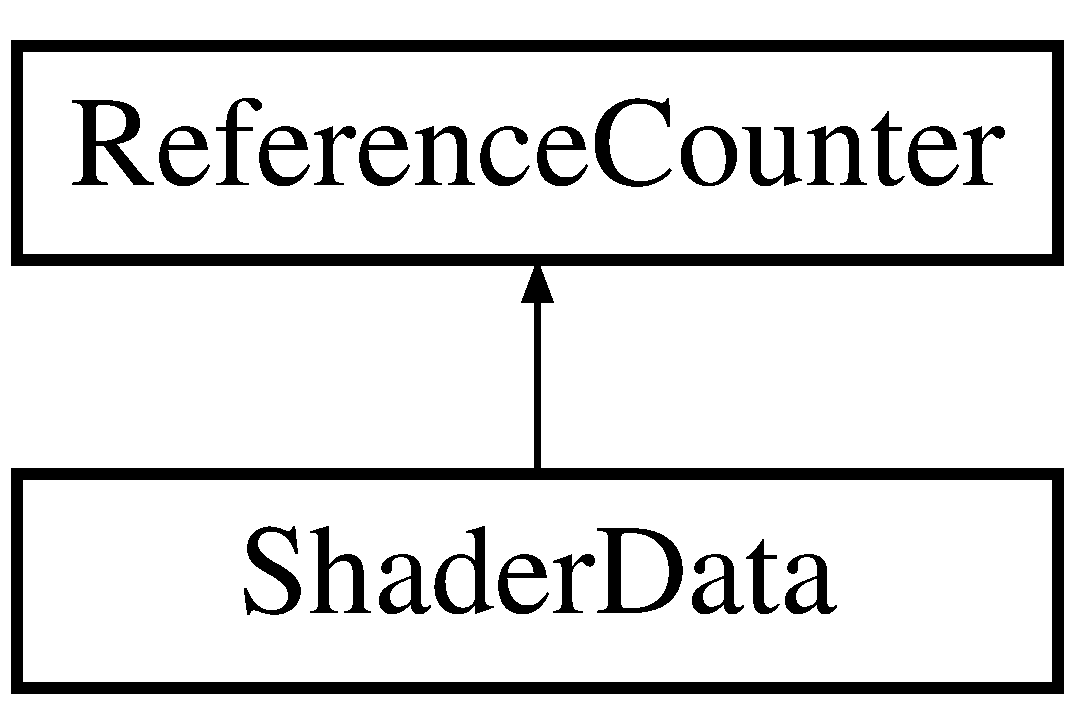
\includegraphics[height=2.000000cm]{class_shader_data}
\end{center}
\end{figure}
\subsection*{Public Member Functions}
\begin{DoxyCompactItemize}
\item 
\hyperlink{class_shader_data_a635def1584d9fbf143b1ee5941a72cf0}{Shader\+Data} (const std\+::string \&file\+Name)
\item 
virtual \hyperlink{class_shader_data_a592e57f2fd0606dbaafae02219d627e2}{$\sim$\+Shader\+Data} ()
\item 
int \hyperlink{class_shader_data_aadcda4012ddfa9278578b5dff9c7f319}{Get\+Program} () const 
\item 
const std\+::vector$<$ int $>$ \& \hyperlink{class_shader_data_addf621db43c86044b38cd2ec404f35dc}{Get\+Shaders} () const 
\item 
const std\+::vector$<$ std\+::string $>$ \& \hyperlink{class_shader_data_a85e13a7e25b6aa859f3e8bda3044422f}{Get\+Uniform\+Names} () const 
\item 
const std\+::vector$<$ std\+::string $>$ \& \hyperlink{class_shader_data_a9f61726bac2a582284fc5f3b9b676af1}{Get\+Uniform\+Types} () const 
\item 
const std\+::map$<$ std\+::string, unsigned int $>$ \& \hyperlink{class_shader_data_a6cde21590e0894121dc02bc50a01f467}{Get\+Uniform\+Map} () const 
\end{DoxyCompactItemize}


\subsection{Constructor \& Destructor Documentation}
\hypertarget{class_shader_data_a635def1584d9fbf143b1ee5941a72cf0}{}\index{Shader\+Data@{Shader\+Data}!Shader\+Data@{Shader\+Data}}
\index{Shader\+Data@{Shader\+Data}!Shader\+Data@{Shader\+Data}}
\subsubsection[{Shader\+Data(const std\+::string \&file\+Name)}]{\setlength{\rightskip}{0pt plus 5cm}Shader\+Data\+::\+Shader\+Data (
\begin{DoxyParamCaption}
\item[{const std\+::string \&}]{file\+Name}
\end{DoxyParamCaption}
)}\label{class_shader_data_a635def1584d9fbf143b1ee5941a72cf0}
\hypertarget{class_shader_data_a592e57f2fd0606dbaafae02219d627e2}{}\index{Shader\+Data@{Shader\+Data}!````~Shader\+Data@{$\sim$\+Shader\+Data}}
\index{````~Shader\+Data@{$\sim$\+Shader\+Data}!Shader\+Data@{Shader\+Data}}
\subsubsection[{$\sim$\+Shader\+Data()}]{\setlength{\rightskip}{0pt plus 5cm}Shader\+Data\+::$\sim$\+Shader\+Data (
\begin{DoxyParamCaption}
{}
\end{DoxyParamCaption}
)\hspace{0.3cm}{\ttfamily [virtual]}}\label{class_shader_data_a592e57f2fd0606dbaafae02219d627e2}


\subsection{Member Function Documentation}
\hypertarget{class_shader_data_aadcda4012ddfa9278578b5dff9c7f319}{}\index{Shader\+Data@{Shader\+Data}!Get\+Program@{Get\+Program}}
\index{Get\+Program@{Get\+Program}!Shader\+Data@{Shader\+Data}}
\subsubsection[{Get\+Program() const }]{\setlength{\rightskip}{0pt plus 5cm}int Shader\+Data\+::\+Get\+Program (
\begin{DoxyParamCaption}
{}
\end{DoxyParamCaption}
) const\hspace{0.3cm}{\ttfamily [inline]}}\label{class_shader_data_aadcda4012ddfa9278578b5dff9c7f319}
\hypertarget{class_shader_data_addf621db43c86044b38cd2ec404f35dc}{}\index{Shader\+Data@{Shader\+Data}!Get\+Shaders@{Get\+Shaders}}
\index{Get\+Shaders@{Get\+Shaders}!Shader\+Data@{Shader\+Data}}
\subsubsection[{Get\+Shaders() const }]{\setlength{\rightskip}{0pt plus 5cm}const std\+::vector$<$int$>$\& Shader\+Data\+::\+Get\+Shaders (
\begin{DoxyParamCaption}
{}
\end{DoxyParamCaption}
) const\hspace{0.3cm}{\ttfamily [inline]}}\label{class_shader_data_addf621db43c86044b38cd2ec404f35dc}
\hypertarget{class_shader_data_a6cde21590e0894121dc02bc50a01f467}{}\index{Shader\+Data@{Shader\+Data}!Get\+Uniform\+Map@{Get\+Uniform\+Map}}
\index{Get\+Uniform\+Map@{Get\+Uniform\+Map}!Shader\+Data@{Shader\+Data}}
\subsubsection[{Get\+Uniform\+Map() const }]{\setlength{\rightskip}{0pt plus 5cm}const std\+::map$<$std\+::string, unsigned int$>$\& Shader\+Data\+::\+Get\+Uniform\+Map (
\begin{DoxyParamCaption}
{}
\end{DoxyParamCaption}
) const\hspace{0.3cm}{\ttfamily [inline]}}\label{class_shader_data_a6cde21590e0894121dc02bc50a01f467}
\hypertarget{class_shader_data_a85e13a7e25b6aa859f3e8bda3044422f}{}\index{Shader\+Data@{Shader\+Data}!Get\+Uniform\+Names@{Get\+Uniform\+Names}}
\index{Get\+Uniform\+Names@{Get\+Uniform\+Names}!Shader\+Data@{Shader\+Data}}
\subsubsection[{Get\+Uniform\+Names() const }]{\setlength{\rightskip}{0pt plus 5cm}const std\+::vector$<$std\+::string$>$\& Shader\+Data\+::\+Get\+Uniform\+Names (
\begin{DoxyParamCaption}
{}
\end{DoxyParamCaption}
) const\hspace{0.3cm}{\ttfamily [inline]}}\label{class_shader_data_a85e13a7e25b6aa859f3e8bda3044422f}
\hypertarget{class_shader_data_a9f61726bac2a582284fc5f3b9b676af1}{}\index{Shader\+Data@{Shader\+Data}!Get\+Uniform\+Types@{Get\+Uniform\+Types}}
\index{Get\+Uniform\+Types@{Get\+Uniform\+Types}!Shader\+Data@{Shader\+Data}}
\subsubsection[{Get\+Uniform\+Types() const }]{\setlength{\rightskip}{0pt plus 5cm}const std\+::vector$<$std\+::string$>$\& Shader\+Data\+::\+Get\+Uniform\+Types (
\begin{DoxyParamCaption}
{}
\end{DoxyParamCaption}
) const\hspace{0.3cm}{\ttfamily [inline]}}\label{class_shader_data_a9f61726bac2a582284fc5f3b9b676af1}


The documentation for this class was generated from the following files\+:\begin{DoxyCompactItemize}
\item 
F\+:/\+Fusion3\+D\+\_\+work/src/rendering/\hyperlink{shader_8h}{shader.\+h}\item 
F\+:/\+Fusion3\+D\+\_\+work/src/rendering/\hyperlink{shader_8cpp}{shader.\+cpp}\end{DoxyCompactItemize}

\hypertarget{class_shadow_camera_transform}{}\section{Shadow\+Camera\+Transform Class Reference}
\label{class_shadow_camera_transform}\index{Shadow\+Camera\+Transform@{Shadow\+Camera\+Transform}}


{\ttfamily \#include $<$lighting.\+h$>$}

\subsection*{Public Member Functions}
\begin{DoxyCompactItemize}
\item 
\hyperlink{class_shadow_camera_transform_aaf1037ea90d5713160422e2ac58b964f}{Shadow\+Camera\+Transform} (const \hyperlink{class_vector3f}{Vector3f} \&pos, const \hyperlink{class_quaternion}{Quaternion} \&rot)
\item 
const \hyperlink{class_vector3f}{Vector3f} \& \hyperlink{class_shadow_camera_transform_afdbf1c1c3fcde59b5487c0ebde21e61d}{Get\+Pos} () const 
\item 
const \hyperlink{class_quaternion}{Quaternion} \& \hyperlink{class_shadow_camera_transform_ab91e6514ae379b5e78cd7905e1aa8f4f}{Get\+Rot} () const 
\end{DoxyCompactItemize}


\subsection{Constructor \& Destructor Documentation}
\hypertarget{class_shadow_camera_transform_aaf1037ea90d5713160422e2ac58b964f}{}\index{Shadow\+Camera\+Transform@{Shadow\+Camera\+Transform}!Shadow\+Camera\+Transform@{Shadow\+Camera\+Transform}}
\index{Shadow\+Camera\+Transform@{Shadow\+Camera\+Transform}!Shadow\+Camera\+Transform@{Shadow\+Camera\+Transform}}
\subsubsection[{Shadow\+Camera\+Transform(const Vector3f \&pos, const Quaternion \&rot)}]{\setlength{\rightskip}{0pt plus 5cm}Shadow\+Camera\+Transform\+::\+Shadow\+Camera\+Transform (
\begin{DoxyParamCaption}
\item[{const {\bf Vector3f} \&}]{pos, }
\item[{const {\bf Quaternion} \&}]{rot}
\end{DoxyParamCaption}
)\hspace{0.3cm}{\ttfamily [inline]}}\label{class_shadow_camera_transform_aaf1037ea90d5713160422e2ac58b964f}


\subsection{Member Function Documentation}
\hypertarget{class_shadow_camera_transform_afdbf1c1c3fcde59b5487c0ebde21e61d}{}\index{Shadow\+Camera\+Transform@{Shadow\+Camera\+Transform}!Get\+Pos@{Get\+Pos}}
\index{Get\+Pos@{Get\+Pos}!Shadow\+Camera\+Transform@{Shadow\+Camera\+Transform}}
\subsubsection[{Get\+Pos() const }]{\setlength{\rightskip}{0pt plus 5cm}const {\bf Vector3f}\& Shadow\+Camera\+Transform\+::\+Get\+Pos (
\begin{DoxyParamCaption}
{}
\end{DoxyParamCaption}
) const\hspace{0.3cm}{\ttfamily [inline]}}\label{class_shadow_camera_transform_afdbf1c1c3fcde59b5487c0ebde21e61d}
\hypertarget{class_shadow_camera_transform_ab91e6514ae379b5e78cd7905e1aa8f4f}{}\index{Shadow\+Camera\+Transform@{Shadow\+Camera\+Transform}!Get\+Rot@{Get\+Rot}}
\index{Get\+Rot@{Get\+Rot}!Shadow\+Camera\+Transform@{Shadow\+Camera\+Transform}}
\subsubsection[{Get\+Rot() const }]{\setlength{\rightskip}{0pt plus 5cm}const {\bf Quaternion}\& Shadow\+Camera\+Transform\+::\+Get\+Rot (
\begin{DoxyParamCaption}
{}
\end{DoxyParamCaption}
) const\hspace{0.3cm}{\ttfamily [inline]}}\label{class_shadow_camera_transform_ab91e6514ae379b5e78cd7905e1aa8f4f}


The documentation for this class was generated from the following file\+:\begin{DoxyCompactItemize}
\item 
F\+:/\+Fusion3\+D\+\_\+work/src/rendering/\hyperlink{lighting_8h}{lighting.\+h}\end{DoxyCompactItemize}

\hypertarget{class_shadow_info}{}\section{Shadow\+Info Class Reference}
\label{class_shadow_info}\index{Shadow\+Info@{Shadow\+Info}}


{\ttfamily \#include $<$lighting.\+h$>$}

\subsection*{Public Member Functions}
\begin{DoxyCompactItemize}
\item 
\hyperlink{class_shadow_info_a1a045ae8bb80275b8f3d1b6659d866ef}{Shadow\+Info} (const \hyperlink{math3d_8h_a5b7721ab7216c91a40538beaa9e6ee1f}{Matrix4f} \&projection=\hyperlink{math3d_8h_a5b7721ab7216c91a40538beaa9e6ee1f}{Matrix4f}().Init\+Identity(), bool flip\+Faces=false, int shadow\+Map\+Size\+As\+Power\+Of2=0, float shadow\+Softness=1.\+0f, float light\+Bleed\+Reduction\+Amount=0.\+2f, float min\+Variance=0.\+00002f)
\item 
const \hyperlink{math3d_8h_a5b7721ab7216c91a40538beaa9e6ee1f}{Matrix4f} \& \hyperlink{class_shadow_info_a49808d2702d996196437f9589ba9514a}{Get\+Projection} () const 
\item 
bool \hyperlink{class_shadow_info_aa80719228d235861516931f7d35f670b}{Get\+Flip\+Faces} () const 
\item 
int \hyperlink{class_shadow_info_abea1d0fde696f23f18545a381ed4e74b}{Get\+Shadow\+Map\+Size\+As\+Power\+Of2} () const 
\item 
float \hyperlink{class_shadow_info_a6d0d788b0bc08483ba4f0ad4e40fcea1}{Get\+Shadow\+Softness} () const 
\item 
float \hyperlink{class_shadow_info_a23944aadb4f86e76626cb1644f525b97}{Get\+Min\+Variance} () const 
\item 
float \hyperlink{class_shadow_info_a1f162e2a842c8ec301847ca25a4277b7}{Get\+Light\+Bleed\+Reduction\+Amount} () const 
\end{DoxyCompactItemize}


\subsection{Constructor \& Destructor Documentation}
\hypertarget{class_shadow_info_a1a045ae8bb80275b8f3d1b6659d866ef}{}\index{Shadow\+Info@{Shadow\+Info}!Shadow\+Info@{Shadow\+Info}}
\index{Shadow\+Info@{Shadow\+Info}!Shadow\+Info@{Shadow\+Info}}
\subsubsection[{Shadow\+Info(const Matrix4f \&projection=\+Matrix4f().\+Init\+Identity(), bool flip\+Faces=false, int shadow\+Map\+Size\+As\+Power\+Of2=0, float shadow\+Softness=1.\+0f, float light\+Bleed\+Reduction\+Amount=0.\+2f, float min\+Variance=0.\+00002f)}]{\setlength{\rightskip}{0pt plus 5cm}Shadow\+Info\+::\+Shadow\+Info (
\begin{DoxyParamCaption}
\item[{const {\bf Matrix4f} \&}]{projection = {\ttfamily {\bf Matrix4f}().InitIdentity()}, }
\item[{bool}]{flip\+Faces = {\ttfamily false}, }
\item[{int}]{shadow\+Map\+Size\+As\+Power\+Of2 = {\ttfamily 0}, }
\item[{float}]{shadow\+Softness = {\ttfamily 1.0f}, }
\item[{float}]{light\+Bleed\+Reduction\+Amount = {\ttfamily 0.2f}, }
\item[{float}]{min\+Variance = {\ttfamily 0.00002f}}
\end{DoxyParamCaption}
)\hspace{0.3cm}{\ttfamily [inline]}}\label{class_shadow_info_a1a045ae8bb80275b8f3d1b6659d866ef}


\subsection{Member Function Documentation}
\hypertarget{class_shadow_info_aa80719228d235861516931f7d35f670b}{}\index{Shadow\+Info@{Shadow\+Info}!Get\+Flip\+Faces@{Get\+Flip\+Faces}}
\index{Get\+Flip\+Faces@{Get\+Flip\+Faces}!Shadow\+Info@{Shadow\+Info}}
\subsubsection[{Get\+Flip\+Faces() const }]{\setlength{\rightskip}{0pt plus 5cm}bool Shadow\+Info\+::\+Get\+Flip\+Faces (
\begin{DoxyParamCaption}
{}
\end{DoxyParamCaption}
) const\hspace{0.3cm}{\ttfamily [inline]}}\label{class_shadow_info_aa80719228d235861516931f7d35f670b}
\hypertarget{class_shadow_info_a1f162e2a842c8ec301847ca25a4277b7}{}\index{Shadow\+Info@{Shadow\+Info}!Get\+Light\+Bleed\+Reduction\+Amount@{Get\+Light\+Bleed\+Reduction\+Amount}}
\index{Get\+Light\+Bleed\+Reduction\+Amount@{Get\+Light\+Bleed\+Reduction\+Amount}!Shadow\+Info@{Shadow\+Info}}
\subsubsection[{Get\+Light\+Bleed\+Reduction\+Amount() const }]{\setlength{\rightskip}{0pt plus 5cm}float Shadow\+Info\+::\+Get\+Light\+Bleed\+Reduction\+Amount (
\begin{DoxyParamCaption}
{}
\end{DoxyParamCaption}
) const\hspace{0.3cm}{\ttfamily [inline]}}\label{class_shadow_info_a1f162e2a842c8ec301847ca25a4277b7}
\hypertarget{class_shadow_info_a23944aadb4f86e76626cb1644f525b97}{}\index{Shadow\+Info@{Shadow\+Info}!Get\+Min\+Variance@{Get\+Min\+Variance}}
\index{Get\+Min\+Variance@{Get\+Min\+Variance}!Shadow\+Info@{Shadow\+Info}}
\subsubsection[{Get\+Min\+Variance() const }]{\setlength{\rightskip}{0pt plus 5cm}float Shadow\+Info\+::\+Get\+Min\+Variance (
\begin{DoxyParamCaption}
{}
\end{DoxyParamCaption}
) const\hspace{0.3cm}{\ttfamily [inline]}}\label{class_shadow_info_a23944aadb4f86e76626cb1644f525b97}
\hypertarget{class_shadow_info_a49808d2702d996196437f9589ba9514a}{}\index{Shadow\+Info@{Shadow\+Info}!Get\+Projection@{Get\+Projection}}
\index{Get\+Projection@{Get\+Projection}!Shadow\+Info@{Shadow\+Info}}
\subsubsection[{Get\+Projection() const }]{\setlength{\rightskip}{0pt plus 5cm}const {\bf Matrix4f}\& Shadow\+Info\+::\+Get\+Projection (
\begin{DoxyParamCaption}
{}
\end{DoxyParamCaption}
) const\hspace{0.3cm}{\ttfamily [inline]}}\label{class_shadow_info_a49808d2702d996196437f9589ba9514a}
\hypertarget{class_shadow_info_abea1d0fde696f23f18545a381ed4e74b}{}\index{Shadow\+Info@{Shadow\+Info}!Get\+Shadow\+Map\+Size\+As\+Power\+Of2@{Get\+Shadow\+Map\+Size\+As\+Power\+Of2}}
\index{Get\+Shadow\+Map\+Size\+As\+Power\+Of2@{Get\+Shadow\+Map\+Size\+As\+Power\+Of2}!Shadow\+Info@{Shadow\+Info}}
\subsubsection[{Get\+Shadow\+Map\+Size\+As\+Power\+Of2() const }]{\setlength{\rightskip}{0pt plus 5cm}int Shadow\+Info\+::\+Get\+Shadow\+Map\+Size\+As\+Power\+Of2 (
\begin{DoxyParamCaption}
{}
\end{DoxyParamCaption}
) const\hspace{0.3cm}{\ttfamily [inline]}}\label{class_shadow_info_abea1d0fde696f23f18545a381ed4e74b}
\hypertarget{class_shadow_info_a6d0d788b0bc08483ba4f0ad4e40fcea1}{}\index{Shadow\+Info@{Shadow\+Info}!Get\+Shadow\+Softness@{Get\+Shadow\+Softness}}
\index{Get\+Shadow\+Softness@{Get\+Shadow\+Softness}!Shadow\+Info@{Shadow\+Info}}
\subsubsection[{Get\+Shadow\+Softness() const }]{\setlength{\rightskip}{0pt plus 5cm}float Shadow\+Info\+::\+Get\+Shadow\+Softness (
\begin{DoxyParamCaption}
{}
\end{DoxyParamCaption}
) const\hspace{0.3cm}{\ttfamily [inline]}}\label{class_shadow_info_a6d0d788b0bc08483ba4f0ad4e40fcea1}


The documentation for this class was generated from the following file\+:\begin{DoxyCompactItemize}
\item 
F\+:/\+Fusion3\+D\+\_\+work/src/rendering/\hyperlink{lighting_8h}{lighting.\+h}\end{DoxyCompactItemize}

\hypertarget{class_s_i_m_d4f}{}\section{S\+I\+M\+D4f Class Reference}
\label{class_s_i_m_d4f}\index{S\+I\+M\+D4f@{S\+I\+M\+D4f}}


{\ttfamily \#include $<$simdemulator.\+h$>$}

\subsection*{Public Member Functions}
\begin{DoxyCompactItemize}
\item 
\hyperlink{class_s_i_m_d4f_abda4aa81a62d1573aba11dcd1e381864}{S\+I\+M\+D4f} ()
\item 
\hyperlink{class_s_i_m_d4f_a9997f26840dc7bfb7eeb818c9a87d367}{S\+I\+M\+D4f} (float a, float b, float c, float d)
\item 
\hyperlink{class_s_i_m_d4f_a10e3822b07aad4fb7988762107cd9234}{S\+I\+M\+D4f} (float a)
\item 
\hyperlink{class_s_i_m_d4f_a744835741d77ed146794c8d8d2b396f7}{S\+I\+M\+D4f} (const float $\ast$data)
\item 
void \hyperlink{class_s_i_m_d4f_a8cd99451df52ad40c4dfdd79a63364bd}{Get} (float $\ast$result) const 
\item 
void \hyperlink{class_s_i_m_d4f_aa023e7d4ac74e0f9a4aecd0795958583}{Set} (const float $\ast$data)
\item 
void \hyperlink{class_s_i_m_d4f_ab22b61011c8d8fa4007025018a97ef17}{Get\+Bytes} (\hyperlink{simddefines_8h_aef44329758059c91c76d334e8fc09700}{int8\+\_\+t} $\ast$result) const 
\item 
void \hyperlink{class_s_i_m_d4f_a4e6d88bddd43495f3c3fa94f4ae1f54c}{Set\+Bytes} (const \hyperlink{simddefines_8h_aef44329758059c91c76d334e8fc09700}{int8\+\_\+t} $\ast$data)
\item 
\hyperlink{class_s_i_m_d4f}{S\+I\+M\+D4f} \hyperlink{class_s_i_m_d4f_a08c9afbd07340f8f094c7337683fdc9f}{And\+Not} (const \hyperlink{class_s_i_m_d4f}{S\+I\+M\+D4f} \&other) const 
\item 
\hyperlink{class_s_i_m_d4f}{S\+I\+M\+D4f} \hyperlink{class_s_i_m_d4f_ac6e26ef1ca79d1e7c65e52899c2869cb}{Max} (const \hyperlink{class_s_i_m_d4f}{S\+I\+M\+D4f} \&other) const 
\item 
\hyperlink{class_s_i_m_d4f}{S\+I\+M\+D4f} \hyperlink{class_s_i_m_d4f_a939bad777bd0c1852d55dcb220b40f68}{Min} (const \hyperlink{class_s_i_m_d4f}{S\+I\+M\+D4f} \&other) const 
\item 
\hyperlink{class_s_i_m_d4f}{S\+I\+M\+D4f} \hyperlink{class_s_i_m_d4f_a2eb197707b1e028665b4ab5399b98e58}{Pick} (const \hyperlink{class_s_i_m_d4f}{S\+I\+M\+D4f} \&source\+If\+True, const \hyperlink{class_s_i_m_d4f}{S\+I\+M\+D4f} \&source\+If\+False)
\item 
\hyperlink{class_s_i_m_d4f}{S\+I\+M\+D4f} \hyperlink{class_s_i_m_d4f_a076452ebd64a5f9321250fca245cbfbc}{Conditional\+Add} (const \hyperlink{class_s_i_m_d4f}{S\+I\+M\+D4f} \&num1, const \hyperlink{class_s_i_m_d4f}{S\+I\+M\+D4f} \&num2)
\item 
\hyperlink{class_s_i_m_d4f}{S\+I\+M\+D4f} \hyperlink{class_s_i_m_d4f_ad295a893eafcfd63abb66cda02192ad0}{Shuffle} (\hyperlink{simddefines_8h_aef44329758059c91c76d334e8fc09700}{int8\+\_\+t} shuffle\+Byte)
\item 
float \hyperlink{class_s_i_m_d4f_a817d0e6bbe46b7dd609188ee73448218}{Horizontal\+Add} () const 
\item 
\hyperlink{class_s_i_m_d4i}{S\+I\+M\+D4i} \hyperlink{class_s_i_m_d4f_afdead05a92f34598d362975c7ec1661c}{Round\+To\+Int} () const 
\item 
\hyperlink{class_s_i_m_d4i}{S\+I\+M\+D4i} \hyperlink{class_s_i_m_d4f_af3630cd24a3be6ca8485d858a1306440}{Truncate\+To\+Int} () const 
\item 
\hyperlink{class_s_i_m_d4f}{S\+I\+M\+D4f} \hyperlink{class_s_i_m_d4f_a6aae2c276b8194b8d3c8ff4c9f6c619e}{Round} (int rounding\+Mode=0) const 
\item 
\hyperlink{class_s_i_m_d4f}{S\+I\+M\+D4f} \hyperlink{class_s_i_m_d4f_a6687bf362a488251b8c5c495cfb2a385}{Floor} () const 
\item 
\hyperlink{class_s_i_m_d4f}{S\+I\+M\+D4f} \hyperlink{class_s_i_m_d4f_a8eec4c908f66003bb8bf1067a6c59bba}{Ceil} () const 
\item 
\hyperlink{class_s_i_m_d4f}{S\+I\+M\+D4f} \hyperlink{class_s_i_m_d4f_a80d9698aefb6ddcefde55b077ee22e2e}{Truncate} () const 
\item 
\hyperlink{class_s_i_m_d4f}{S\+I\+M\+D4f} \hyperlink{class_s_i_m_d4f_a57b0c4d2e3dee7a7463040c76f9d34bd}{Abs} () const 
\item 
\hyperlink{class_s_i_m_d4f}{S\+I\+M\+D4f} \hyperlink{class_s_i_m_d4f_a510350c7a4ed579fd9c143bd059e6e05}{Sqrt} () const 
\item 
\hyperlink{class_s_i_m_d4f}{S\+I\+M\+D4f} \hyperlink{class_s_i_m_d4f_a40f4dbbc2538ba8bd8d92c18e617ee59}{Fast\+R\+Sqrt} () const 
\item 
\hyperlink{class_s_i_m_d4f}{S\+I\+M\+D4f} \hyperlink{class_s_i_m_d4f_aee80a83cd05cbfe0062b4d6935d2d7b8}{Fast\+Reciprocal} () const 
\item 
\hyperlink{class_s_i_m_d4f}{S\+I\+M\+D4f} \hyperlink{class_s_i_m_d4f_a37059580a943f034510927272fa06c38}{operator+} (const \hyperlink{class_s_i_m_d4f}{S\+I\+M\+D4f} \&other) const 
\item 
void \hyperlink{class_s_i_m_d4f_ab547cee5fcc6f68c1e5e74c9e14cd564}{operator+=} (const \hyperlink{class_s_i_m_d4f}{S\+I\+M\+D4f} \&other)
\item 
\hyperlink{class_s_i_m_d4f}{S\+I\+M\+D4f} \hyperlink{class_s_i_m_d4f_a35950395f46f9e1e07e949ade9664876}{operator-\/} (const \hyperlink{class_s_i_m_d4f}{S\+I\+M\+D4f} \&other) const 
\item 
void \hyperlink{class_s_i_m_d4f_a6b83a005afad9d0cbafd6aa91387fbc5}{operator-\/=} (const \hyperlink{class_s_i_m_d4f}{S\+I\+M\+D4f} \&other)
\item 
\hyperlink{class_s_i_m_d4f}{S\+I\+M\+D4f} \hyperlink{class_s_i_m_d4f_a7c3566f2b6ec0dba55e889dcbadd48f0}{operator$\ast$} (const \hyperlink{class_s_i_m_d4f}{S\+I\+M\+D4f} \&other) const 
\item 
void \hyperlink{class_s_i_m_d4f_a6a74b6d3b0681777b34e3de2b47110c6}{operator$\ast$=} (const \hyperlink{class_s_i_m_d4f}{S\+I\+M\+D4f} \&other)
\item 
\hyperlink{class_s_i_m_d4f}{S\+I\+M\+D4f} \hyperlink{class_s_i_m_d4f_a8eb9f3ee0c70ef4569a875aead8b4985}{operator/} (const \hyperlink{class_s_i_m_d4f}{S\+I\+M\+D4f} \&other) const 
\item 
void \hyperlink{class_s_i_m_d4f_a3b6b3c49cfd05e88a3cb69edeef75b6c}{operator/=} (const \hyperlink{class_s_i_m_d4f}{S\+I\+M\+D4f} \&other)
\item 
\hyperlink{class_s_i_m_d4f}{S\+I\+M\+D4f} \hyperlink{class_s_i_m_d4f_a1df8ad0c155adc333d43da786c7fcc69}{operator\&} (const \hyperlink{class_s_i_m_d4f}{S\+I\+M\+D4f} \&other) const 
\item 
void \hyperlink{class_s_i_m_d4f_a870101dc4dff1951f6aa74b01dbd875d}{operator\&=} (const \hyperlink{class_s_i_m_d4f}{S\+I\+M\+D4f} \&other)
\item 
\hyperlink{class_s_i_m_d4f}{S\+I\+M\+D4f} \hyperlink{class_s_i_m_d4f_ae2364977959dbd7e38cfad50b449dab5}{operator$\vert$} (const \hyperlink{class_s_i_m_d4f}{S\+I\+M\+D4f} \&other) const 
\item 
void \hyperlink{class_s_i_m_d4f_a8ff9a65196ceec407c9b3f4adf3a1911}{operator$\vert$=} (const \hyperlink{class_s_i_m_d4f}{S\+I\+M\+D4f} \&other)
\item 
\hyperlink{class_s_i_m_d4f}{S\+I\+M\+D4f} \hyperlink{class_s_i_m_d4f_a0aac563f1f7e9326b84a78d04995041a}{operator$^\wedge$} (const \hyperlink{class_s_i_m_d4f}{S\+I\+M\+D4f} \&other) const 
\item 
void \hyperlink{class_s_i_m_d4f_a27c17c6b57f44045fb33c0427e33210b}{operator$^\wedge$=} (const \hyperlink{class_s_i_m_d4f}{S\+I\+M\+D4f} \&other)
\item 
\hyperlink{class_s_i_m_d4f}{S\+I\+M\+D4f} \hyperlink{class_s_i_m_d4f_ade3596e82e7765959b1c4d88b6677d5e}{operator==} (const \hyperlink{class_s_i_m_d4f}{S\+I\+M\+D4f} \&other) const 
\item 
\hyperlink{class_s_i_m_d4f}{S\+I\+M\+D4f} \hyperlink{class_s_i_m_d4f_a57b8179ec1d84168c1652b5426fa3a23}{operator!=} (const \hyperlink{class_s_i_m_d4f}{S\+I\+M\+D4f} \&other) const 
\item 
\hyperlink{class_s_i_m_d4f}{S\+I\+M\+D4f} \hyperlink{class_s_i_m_d4f_aa82f83875606b53854dda2484561c435}{operator$>$} (const \hyperlink{class_s_i_m_d4f}{S\+I\+M\+D4f} \&other) const 
\item 
\hyperlink{class_s_i_m_d4f}{S\+I\+M\+D4f} \hyperlink{class_s_i_m_d4f_ad94926234ab8e74f007d137135ef6990}{operator$<$} (const \hyperlink{class_s_i_m_d4f}{S\+I\+M\+D4f} \&other) const 
\item 
\hyperlink{class_s_i_m_d4f}{S\+I\+M\+D4f} \hyperlink{class_s_i_m_d4f_ab335c298dcef73b1e1e67500bfc5cbea}{operator$>$=} (const \hyperlink{class_s_i_m_d4f}{S\+I\+M\+D4f} \&other) const 
\item 
\hyperlink{class_s_i_m_d4f}{S\+I\+M\+D4f} \hyperlink{class_s_i_m_d4f_a58edb1a5141a88422c789201633c22fc}{operator$<$=} (const \hyperlink{class_s_i_m_d4f}{S\+I\+M\+D4f} \&other) const 
\item 
\hyperlink{class_s_i_m_d4f}{S\+I\+M\+D4f} \hyperlink{class_s_i_m_d4f_af9f8304a6372911aae73c04bae766dc8}{operator!} () const 
\item 
\hyperlink{class_s_i_m_d4f_abda4aa81a62d1573aba11dcd1e381864}{S\+I\+M\+D4f} ()
\item 
\hyperlink{class_s_i_m_d4f_a9997f26840dc7bfb7eeb818c9a87d367}{S\+I\+M\+D4f} (float a, float b, float c, float d)
\item 
\hyperlink{class_s_i_m_d4f_a10e3822b07aad4fb7988762107cd9234}{S\+I\+M\+D4f} (float a)
\item 
\hyperlink{class_s_i_m_d4f_ac549a6be599e9f749ad55cb02c3eb6d4}{S\+I\+M\+D4f} (const \+\_\+\+\_\+m128 \&data)
\item 
void \hyperlink{class_s_i_m_d4f_a8cd99451df52ad40c4dfdd79a63364bd}{Get} (float $\ast$result) const 
\item 
void \hyperlink{class_s_i_m_d4f_aa023e7d4ac74e0f9a4aecd0795958583}{Set} (const float $\ast$data)
\item 
void \hyperlink{class_s_i_m_d4f_ab22b61011c8d8fa4007025018a97ef17}{Get\+Bytes} (\hyperlink{simddefines_8h_aef44329758059c91c76d334e8fc09700}{int8\+\_\+t} $\ast$result) const 
\item 
void \hyperlink{class_s_i_m_d4f_a4e6d88bddd43495f3c3fa94f4ae1f54c}{Set\+Bytes} (const \hyperlink{simddefines_8h_aef44329758059c91c76d334e8fc09700}{int8\+\_\+t} $\ast$data)
\item 
\hyperlink{class_s_i_m_d4f}{S\+I\+M\+D4f} \hyperlink{class_s_i_m_d4f_a08c9afbd07340f8f094c7337683fdc9f}{And\+Not} (const \hyperlink{class_s_i_m_d4f}{S\+I\+M\+D4f} \&other) const 
\item 
\hyperlink{class_s_i_m_d4f}{S\+I\+M\+D4f} \hyperlink{class_s_i_m_d4f_ac6e26ef1ca79d1e7c65e52899c2869cb}{Max} (const \hyperlink{class_s_i_m_d4f}{S\+I\+M\+D4f} \&other) const 
\item 
\hyperlink{class_s_i_m_d4f}{S\+I\+M\+D4f} \hyperlink{class_s_i_m_d4f_a939bad777bd0c1852d55dcb220b40f68}{Min} (const \hyperlink{class_s_i_m_d4f}{S\+I\+M\+D4f} \&other) const 
\item 
\hyperlink{class_s_i_m_d4f}{S\+I\+M\+D4f} \hyperlink{class_s_i_m_d4f_a2eb197707b1e028665b4ab5399b98e58}{Pick} (const \hyperlink{class_s_i_m_d4f}{S\+I\+M\+D4f} \&source\+If\+True, const \hyperlink{class_s_i_m_d4f}{S\+I\+M\+D4f} \&source\+If\+False)
\item 
\hyperlink{class_s_i_m_d4f}{S\+I\+M\+D4f} \hyperlink{class_s_i_m_d4f_a076452ebd64a5f9321250fca245cbfbc}{Conditional\+Add} (const \hyperlink{class_s_i_m_d4f}{S\+I\+M\+D4f} \&num1, const \hyperlink{class_s_i_m_d4f}{S\+I\+M\+D4f} \&num2)
\item 
\hyperlink{class_s_i_m_d4f}{S\+I\+M\+D4f} \hyperlink{class_s_i_m_d4f_ad295a893eafcfd63abb66cda02192ad0}{Shuffle} (\hyperlink{simddefines_8h_aef44329758059c91c76d334e8fc09700}{int8\+\_\+t} shuffle\+Byte)
\item 
float \hyperlink{class_s_i_m_d4f_a817d0e6bbe46b7dd609188ee73448218}{Horizontal\+Add} () const 
\item 
\hyperlink{class_s_i_m_d4i}{S\+I\+M\+D4i} \hyperlink{class_s_i_m_d4f_afdead05a92f34598d362975c7ec1661c}{Round\+To\+Int} () const 
\item 
\hyperlink{class_s_i_m_d4i}{S\+I\+M\+D4i} \hyperlink{class_s_i_m_d4f_af3630cd24a3be6ca8485d858a1306440}{Truncate\+To\+Int} () const 
\item 
\hyperlink{class_s_i_m_d4f}{S\+I\+M\+D4f} \hyperlink{class_s_i_m_d4f_a6aae2c276b8194b8d3c8ff4c9f6c619e}{Round} (int rounding\+Mode=0) const 
\item 
\hyperlink{class_s_i_m_d4f}{S\+I\+M\+D4f} \hyperlink{class_s_i_m_d4f_a6687bf362a488251b8c5c495cfb2a385}{Floor} () const 
\item 
\hyperlink{class_s_i_m_d4f}{S\+I\+M\+D4f} \hyperlink{class_s_i_m_d4f_a8eec4c908f66003bb8bf1067a6c59bba}{Ceil} () const 
\item 
\hyperlink{class_s_i_m_d4f}{S\+I\+M\+D4f} \hyperlink{class_s_i_m_d4f_a80d9698aefb6ddcefde55b077ee22e2e}{Truncate} () const 
\item 
\hyperlink{class_s_i_m_d4f}{S\+I\+M\+D4f} \hyperlink{class_s_i_m_d4f_a57b0c4d2e3dee7a7463040c76f9d34bd}{Abs} () const 
\item 
\hyperlink{class_s_i_m_d4f}{S\+I\+M\+D4f} \hyperlink{class_s_i_m_d4f_a510350c7a4ed579fd9c143bd059e6e05}{Sqrt} () const 
\item 
\hyperlink{class_s_i_m_d4f}{S\+I\+M\+D4f} \hyperlink{class_s_i_m_d4f_a40f4dbbc2538ba8bd8d92c18e617ee59}{Fast\+R\+Sqrt} () const 
\item 
\hyperlink{class_s_i_m_d4f}{S\+I\+M\+D4f} \hyperlink{class_s_i_m_d4f_aee80a83cd05cbfe0062b4d6935d2d7b8}{Fast\+Reciprocal} () const 
\item 
\hyperlink{class_s_i_m_d4f}{S\+I\+M\+D4f} \hyperlink{class_s_i_m_d4f_a37059580a943f034510927272fa06c38}{operator+} (const \hyperlink{class_s_i_m_d4f}{S\+I\+M\+D4f} \&other) const 
\item 
void \hyperlink{class_s_i_m_d4f_ab547cee5fcc6f68c1e5e74c9e14cd564}{operator+=} (const \hyperlink{class_s_i_m_d4f}{S\+I\+M\+D4f} \&other)
\item 
\hyperlink{class_s_i_m_d4f}{S\+I\+M\+D4f} \hyperlink{class_s_i_m_d4f_a35950395f46f9e1e07e949ade9664876}{operator-\/} (const \hyperlink{class_s_i_m_d4f}{S\+I\+M\+D4f} \&other) const 
\item 
void \hyperlink{class_s_i_m_d4f_a6b83a005afad9d0cbafd6aa91387fbc5}{operator-\/=} (const \hyperlink{class_s_i_m_d4f}{S\+I\+M\+D4f} \&other)
\item 
\hyperlink{class_s_i_m_d4f}{S\+I\+M\+D4f} \hyperlink{class_s_i_m_d4f_a7c3566f2b6ec0dba55e889dcbadd48f0}{operator$\ast$} (const \hyperlink{class_s_i_m_d4f}{S\+I\+M\+D4f} \&other) const 
\item 
void \hyperlink{class_s_i_m_d4f_a6a74b6d3b0681777b34e3de2b47110c6}{operator$\ast$=} (const \hyperlink{class_s_i_m_d4f}{S\+I\+M\+D4f} \&other)
\item 
\hyperlink{class_s_i_m_d4f}{S\+I\+M\+D4f} \hyperlink{class_s_i_m_d4f_a8eb9f3ee0c70ef4569a875aead8b4985}{operator/} (const \hyperlink{class_s_i_m_d4f}{S\+I\+M\+D4f} \&other) const 
\item 
void \hyperlink{class_s_i_m_d4f_a3b6b3c49cfd05e88a3cb69edeef75b6c}{operator/=} (const \hyperlink{class_s_i_m_d4f}{S\+I\+M\+D4f} \&other)
\item 
\hyperlink{class_s_i_m_d4f}{S\+I\+M\+D4f} \hyperlink{class_s_i_m_d4f_a1df8ad0c155adc333d43da786c7fcc69}{operator\&} (const \hyperlink{class_s_i_m_d4f}{S\+I\+M\+D4f} \&other) const 
\item 
void \hyperlink{class_s_i_m_d4f_a870101dc4dff1951f6aa74b01dbd875d}{operator\&=} (const \hyperlink{class_s_i_m_d4f}{S\+I\+M\+D4f} \&other)
\item 
\hyperlink{class_s_i_m_d4f}{S\+I\+M\+D4f} \hyperlink{class_s_i_m_d4f_ae2364977959dbd7e38cfad50b449dab5}{operator$\vert$} (const \hyperlink{class_s_i_m_d4f}{S\+I\+M\+D4f} \&other) const 
\item 
void \hyperlink{class_s_i_m_d4f_a8ff9a65196ceec407c9b3f4adf3a1911}{operator$\vert$=} (const \hyperlink{class_s_i_m_d4f}{S\+I\+M\+D4f} \&other)
\item 
\hyperlink{class_s_i_m_d4f}{S\+I\+M\+D4f} \hyperlink{class_s_i_m_d4f_a0aac563f1f7e9326b84a78d04995041a}{operator$^\wedge$} (const \hyperlink{class_s_i_m_d4f}{S\+I\+M\+D4f} \&other) const 
\item 
void \hyperlink{class_s_i_m_d4f_a27c17c6b57f44045fb33c0427e33210b}{operator$^\wedge$=} (const \hyperlink{class_s_i_m_d4f}{S\+I\+M\+D4f} \&other)
\item 
\hyperlink{class_s_i_m_d4f}{S\+I\+M\+D4f} \hyperlink{class_s_i_m_d4f_ade3596e82e7765959b1c4d88b6677d5e}{operator==} (const \hyperlink{class_s_i_m_d4f}{S\+I\+M\+D4f} \&other) const 
\item 
\hyperlink{class_s_i_m_d4f}{S\+I\+M\+D4f} \hyperlink{class_s_i_m_d4f_a57b8179ec1d84168c1652b5426fa3a23}{operator!=} (const \hyperlink{class_s_i_m_d4f}{S\+I\+M\+D4f} \&other) const 
\item 
\hyperlink{class_s_i_m_d4f}{S\+I\+M\+D4f} \hyperlink{class_s_i_m_d4f_aa82f83875606b53854dda2484561c435}{operator$>$} (const \hyperlink{class_s_i_m_d4f}{S\+I\+M\+D4f} \&other) const 
\item 
\hyperlink{class_s_i_m_d4f}{S\+I\+M\+D4f} \hyperlink{class_s_i_m_d4f_ad94926234ab8e74f007d137135ef6990}{operator$<$} (const \hyperlink{class_s_i_m_d4f}{S\+I\+M\+D4f} \&other) const 
\item 
\hyperlink{class_s_i_m_d4f}{S\+I\+M\+D4f} \hyperlink{class_s_i_m_d4f_ab335c298dcef73b1e1e67500bfc5cbea}{operator$>$=} (const \hyperlink{class_s_i_m_d4f}{S\+I\+M\+D4f} \&other) const 
\item 
\hyperlink{class_s_i_m_d4f}{S\+I\+M\+D4f} \hyperlink{class_s_i_m_d4f_a58edb1a5141a88422c789201633c22fc}{operator$<$=} (const \hyperlink{class_s_i_m_d4f}{S\+I\+M\+D4f} \&other) const 
\item 
\hyperlink{class_s_i_m_d4f}{S\+I\+M\+D4f} \hyperlink{class_s_i_m_d4f_af9f8304a6372911aae73c04bae766dc8}{operator!} () const 
\item 
\hyperlink{class_s_i_m_d4f_aff52214289656c2e89262fe874b5869c}{operator \+\_\+\+\_\+m128} () const 
\end{DoxyCompactItemize}


\subsection{Constructor \& Destructor Documentation}
\hypertarget{class_s_i_m_d4f_abda4aa81a62d1573aba11dcd1e381864}{}\index{S\+I\+M\+D4f@{S\+I\+M\+D4f}!S\+I\+M\+D4f@{S\+I\+M\+D4f}}
\index{S\+I\+M\+D4f@{S\+I\+M\+D4f}!S\+I\+M\+D4f@{S\+I\+M\+D4f}}
\subsubsection[{S\+I\+M\+D4f()}]{\setlength{\rightskip}{0pt plus 5cm}S\+I\+M\+D4f\+::\+S\+I\+M\+D4f (
\begin{DoxyParamCaption}
{}
\end{DoxyParamCaption}
)\hspace{0.3cm}{\ttfamily [inline]}}\label{class_s_i_m_d4f_abda4aa81a62d1573aba11dcd1e381864}
\hypertarget{class_s_i_m_d4f_a9997f26840dc7bfb7eeb818c9a87d367}{}\index{S\+I\+M\+D4f@{S\+I\+M\+D4f}!S\+I\+M\+D4f@{S\+I\+M\+D4f}}
\index{S\+I\+M\+D4f@{S\+I\+M\+D4f}!S\+I\+M\+D4f@{S\+I\+M\+D4f}}
\subsubsection[{S\+I\+M\+D4f(float a, float b, float c, float d)}]{\setlength{\rightskip}{0pt plus 5cm}S\+I\+M\+D4f\+::\+S\+I\+M\+D4f (
\begin{DoxyParamCaption}
\item[{float}]{a, }
\item[{float}]{b, }
\item[{float}]{c, }
\item[{float}]{d}
\end{DoxyParamCaption}
)\hspace{0.3cm}{\ttfamily [inline]}}\label{class_s_i_m_d4f_a9997f26840dc7bfb7eeb818c9a87d367}
\hypertarget{class_s_i_m_d4f_a10e3822b07aad4fb7988762107cd9234}{}\index{S\+I\+M\+D4f@{S\+I\+M\+D4f}!S\+I\+M\+D4f@{S\+I\+M\+D4f}}
\index{S\+I\+M\+D4f@{S\+I\+M\+D4f}!S\+I\+M\+D4f@{S\+I\+M\+D4f}}
\subsubsection[{S\+I\+M\+D4f(float a)}]{\setlength{\rightskip}{0pt plus 5cm}S\+I\+M\+D4f\+::\+S\+I\+M\+D4f (
\begin{DoxyParamCaption}
\item[{float}]{a}
\end{DoxyParamCaption}
)\hspace{0.3cm}{\ttfamily [inline]}}\label{class_s_i_m_d4f_a10e3822b07aad4fb7988762107cd9234}
\hypertarget{class_s_i_m_d4f_a744835741d77ed146794c8d8d2b396f7}{}\index{S\+I\+M\+D4f@{S\+I\+M\+D4f}!S\+I\+M\+D4f@{S\+I\+M\+D4f}}
\index{S\+I\+M\+D4f@{S\+I\+M\+D4f}!S\+I\+M\+D4f@{S\+I\+M\+D4f}}
\subsubsection[{S\+I\+M\+D4f(const float $\ast$data)}]{\setlength{\rightskip}{0pt plus 5cm}S\+I\+M\+D4f\+::\+S\+I\+M\+D4f (
\begin{DoxyParamCaption}
\item[{const float $\ast$}]{data}
\end{DoxyParamCaption}
)\hspace{0.3cm}{\ttfamily [inline]}}\label{class_s_i_m_d4f_a744835741d77ed146794c8d8d2b396f7}
\hypertarget{class_s_i_m_d4f_abda4aa81a62d1573aba11dcd1e381864}{}\index{S\+I\+M\+D4f@{S\+I\+M\+D4f}!S\+I\+M\+D4f@{S\+I\+M\+D4f}}
\index{S\+I\+M\+D4f@{S\+I\+M\+D4f}!S\+I\+M\+D4f@{S\+I\+M\+D4f}}
\subsubsection[{S\+I\+M\+D4f()}]{\setlength{\rightskip}{0pt plus 5cm}S\+I\+M\+D4f\+::\+S\+I\+M\+D4f (
\begin{DoxyParamCaption}
{}
\end{DoxyParamCaption}
)\hspace{0.3cm}{\ttfamily [inline]}}\label{class_s_i_m_d4f_abda4aa81a62d1573aba11dcd1e381864}
\hypertarget{class_s_i_m_d4f_a9997f26840dc7bfb7eeb818c9a87d367}{}\index{S\+I\+M\+D4f@{S\+I\+M\+D4f}!S\+I\+M\+D4f@{S\+I\+M\+D4f}}
\index{S\+I\+M\+D4f@{S\+I\+M\+D4f}!S\+I\+M\+D4f@{S\+I\+M\+D4f}}
\subsubsection[{S\+I\+M\+D4f(float a, float b, float c, float d)}]{\setlength{\rightskip}{0pt plus 5cm}S\+I\+M\+D4f\+::\+S\+I\+M\+D4f (
\begin{DoxyParamCaption}
\item[{float}]{a, }
\item[{float}]{b, }
\item[{float}]{c, }
\item[{float}]{d}
\end{DoxyParamCaption}
)\hspace{0.3cm}{\ttfamily [inline]}}\label{class_s_i_m_d4f_a9997f26840dc7bfb7eeb818c9a87d367}
\hypertarget{class_s_i_m_d4f_a10e3822b07aad4fb7988762107cd9234}{}\index{S\+I\+M\+D4f@{S\+I\+M\+D4f}!S\+I\+M\+D4f@{S\+I\+M\+D4f}}
\index{S\+I\+M\+D4f@{S\+I\+M\+D4f}!S\+I\+M\+D4f@{S\+I\+M\+D4f}}
\subsubsection[{S\+I\+M\+D4f(float a)}]{\setlength{\rightskip}{0pt plus 5cm}S\+I\+M\+D4f\+::\+S\+I\+M\+D4f (
\begin{DoxyParamCaption}
\item[{float}]{a}
\end{DoxyParamCaption}
)\hspace{0.3cm}{\ttfamily [inline]}}\label{class_s_i_m_d4f_a10e3822b07aad4fb7988762107cd9234}
\hypertarget{class_s_i_m_d4f_ac549a6be599e9f749ad55cb02c3eb6d4}{}\index{S\+I\+M\+D4f@{S\+I\+M\+D4f}!S\+I\+M\+D4f@{S\+I\+M\+D4f}}
\index{S\+I\+M\+D4f@{S\+I\+M\+D4f}!S\+I\+M\+D4f@{S\+I\+M\+D4f}}
\subsubsection[{S\+I\+M\+D4f(const \+\_\+\+\_\+m128 \&data)}]{\setlength{\rightskip}{0pt plus 5cm}S\+I\+M\+D4f\+::\+S\+I\+M\+D4f (
\begin{DoxyParamCaption}
\item[{const \+\_\+\+\_\+m128 \&}]{data}
\end{DoxyParamCaption}
)\hspace{0.3cm}{\ttfamily [inline]}}\label{class_s_i_m_d4f_ac549a6be599e9f749ad55cb02c3eb6d4}


\subsection{Member Function Documentation}
\hypertarget{class_s_i_m_d4f_a57b0c4d2e3dee7a7463040c76f9d34bd}{}\index{S\+I\+M\+D4f@{S\+I\+M\+D4f}!Abs@{Abs}}
\index{Abs@{Abs}!S\+I\+M\+D4f@{S\+I\+M\+D4f}}
\subsubsection[{Abs() const }]{\setlength{\rightskip}{0pt plus 5cm}{\bf S\+I\+M\+D4f} S\+I\+M\+D4f\+::\+Abs (
\begin{DoxyParamCaption}
{}
\end{DoxyParamCaption}
) const\hspace{0.3cm}{\ttfamily [inline]}}\label{class_s_i_m_d4f_a57b0c4d2e3dee7a7463040c76f9d34bd}
\hypertarget{class_s_i_m_d4f_a57b0c4d2e3dee7a7463040c76f9d34bd}{}\index{S\+I\+M\+D4f@{S\+I\+M\+D4f}!Abs@{Abs}}
\index{Abs@{Abs}!S\+I\+M\+D4f@{S\+I\+M\+D4f}}
\subsubsection[{Abs() const }]{\setlength{\rightskip}{0pt plus 5cm}{\bf S\+I\+M\+D4f} S\+I\+M\+D4f\+::\+Abs (
\begin{DoxyParamCaption}
{}
\end{DoxyParamCaption}
) const\hspace{0.3cm}{\ttfamily [inline]}}\label{class_s_i_m_d4f_a57b0c4d2e3dee7a7463040c76f9d34bd}
\hypertarget{class_s_i_m_d4f_a08c9afbd07340f8f094c7337683fdc9f}{}\index{S\+I\+M\+D4f@{S\+I\+M\+D4f}!And\+Not@{And\+Not}}
\index{And\+Not@{And\+Not}!S\+I\+M\+D4f@{S\+I\+M\+D4f}}
\subsubsection[{And\+Not(const S\+I\+M\+D4f \&other) const }]{\setlength{\rightskip}{0pt plus 5cm}{\bf S\+I\+M\+D4f} S\+I\+M\+D4f\+::\+And\+Not (
\begin{DoxyParamCaption}
\item[{const {\bf S\+I\+M\+D4f} \&}]{other}
\end{DoxyParamCaption}
) const\hspace{0.3cm}{\ttfamily [inline]}}\label{class_s_i_m_d4f_a08c9afbd07340f8f094c7337683fdc9f}
\hypertarget{class_s_i_m_d4f_a08c9afbd07340f8f094c7337683fdc9f}{}\index{S\+I\+M\+D4f@{S\+I\+M\+D4f}!And\+Not@{And\+Not}}
\index{And\+Not@{And\+Not}!S\+I\+M\+D4f@{S\+I\+M\+D4f}}
\subsubsection[{And\+Not(const S\+I\+M\+D4f \&other) const }]{\setlength{\rightskip}{0pt plus 5cm}{\bf S\+I\+M\+D4f} S\+I\+M\+D4f\+::\+And\+Not (
\begin{DoxyParamCaption}
\item[{const {\bf S\+I\+M\+D4f} \&}]{other}
\end{DoxyParamCaption}
) const\hspace{0.3cm}{\ttfamily [inline]}}\label{class_s_i_m_d4f_a08c9afbd07340f8f094c7337683fdc9f}
\hypertarget{class_s_i_m_d4f_a8eec4c908f66003bb8bf1067a6c59bba}{}\index{S\+I\+M\+D4f@{S\+I\+M\+D4f}!Ceil@{Ceil}}
\index{Ceil@{Ceil}!S\+I\+M\+D4f@{S\+I\+M\+D4f}}
\subsubsection[{Ceil() const }]{\setlength{\rightskip}{0pt plus 5cm}{\bf S\+I\+M\+D4f} S\+I\+M\+D4f\+::\+Ceil (
\begin{DoxyParamCaption}
{}
\end{DoxyParamCaption}
) const\hspace{0.3cm}{\ttfamily [inline]}}\label{class_s_i_m_d4f_a8eec4c908f66003bb8bf1067a6c59bba}
\hypertarget{class_s_i_m_d4f_a8eec4c908f66003bb8bf1067a6c59bba}{}\index{S\+I\+M\+D4f@{S\+I\+M\+D4f}!Ceil@{Ceil}}
\index{Ceil@{Ceil}!S\+I\+M\+D4f@{S\+I\+M\+D4f}}
\subsubsection[{Ceil() const }]{\setlength{\rightskip}{0pt plus 5cm}{\bf S\+I\+M\+D4f} S\+I\+M\+D4f\+::\+Ceil (
\begin{DoxyParamCaption}
{}
\end{DoxyParamCaption}
) const\hspace{0.3cm}{\ttfamily [inline]}}\label{class_s_i_m_d4f_a8eec4c908f66003bb8bf1067a6c59bba}
\hypertarget{class_s_i_m_d4f_a076452ebd64a5f9321250fca245cbfbc}{}\index{S\+I\+M\+D4f@{S\+I\+M\+D4f}!Conditional\+Add@{Conditional\+Add}}
\index{Conditional\+Add@{Conditional\+Add}!S\+I\+M\+D4f@{S\+I\+M\+D4f}}
\subsubsection[{Conditional\+Add(const S\+I\+M\+D4f \&num1, const S\+I\+M\+D4f \&num2)}]{\setlength{\rightskip}{0pt plus 5cm}{\bf S\+I\+M\+D4f} S\+I\+M\+D4f\+::\+Conditional\+Add (
\begin{DoxyParamCaption}
\item[{const {\bf S\+I\+M\+D4f} \&}]{num1, }
\item[{const {\bf S\+I\+M\+D4f} \&}]{num2}
\end{DoxyParamCaption}
)\hspace{0.3cm}{\ttfamily [inline]}}\label{class_s_i_m_d4f_a076452ebd64a5f9321250fca245cbfbc}
\hypertarget{class_s_i_m_d4f_a076452ebd64a5f9321250fca245cbfbc}{}\index{S\+I\+M\+D4f@{S\+I\+M\+D4f}!Conditional\+Add@{Conditional\+Add}}
\index{Conditional\+Add@{Conditional\+Add}!S\+I\+M\+D4f@{S\+I\+M\+D4f}}
\subsubsection[{Conditional\+Add(const S\+I\+M\+D4f \&num1, const S\+I\+M\+D4f \&num2)}]{\setlength{\rightskip}{0pt plus 5cm}{\bf S\+I\+M\+D4f} S\+I\+M\+D4f\+::\+Conditional\+Add (
\begin{DoxyParamCaption}
\item[{const {\bf S\+I\+M\+D4f} \&}]{num1, }
\item[{const {\bf S\+I\+M\+D4f} \&}]{num2}
\end{DoxyParamCaption}
)\hspace{0.3cm}{\ttfamily [inline]}}\label{class_s_i_m_d4f_a076452ebd64a5f9321250fca245cbfbc}
\hypertarget{class_s_i_m_d4f_aee80a83cd05cbfe0062b4d6935d2d7b8}{}\index{S\+I\+M\+D4f@{S\+I\+M\+D4f}!Fast\+Reciprocal@{Fast\+Reciprocal}}
\index{Fast\+Reciprocal@{Fast\+Reciprocal}!S\+I\+M\+D4f@{S\+I\+M\+D4f}}
\subsubsection[{Fast\+Reciprocal() const }]{\setlength{\rightskip}{0pt plus 5cm}{\bf S\+I\+M\+D4f} S\+I\+M\+D4f\+::\+Fast\+Reciprocal (
\begin{DoxyParamCaption}
{}
\end{DoxyParamCaption}
) const\hspace{0.3cm}{\ttfamily [inline]}}\label{class_s_i_m_d4f_aee80a83cd05cbfe0062b4d6935d2d7b8}
\hypertarget{class_s_i_m_d4f_aee80a83cd05cbfe0062b4d6935d2d7b8}{}\index{S\+I\+M\+D4f@{S\+I\+M\+D4f}!Fast\+Reciprocal@{Fast\+Reciprocal}}
\index{Fast\+Reciprocal@{Fast\+Reciprocal}!S\+I\+M\+D4f@{S\+I\+M\+D4f}}
\subsubsection[{Fast\+Reciprocal() const }]{\setlength{\rightskip}{0pt plus 5cm}{\bf S\+I\+M\+D4f} S\+I\+M\+D4f\+::\+Fast\+Reciprocal (
\begin{DoxyParamCaption}
{}
\end{DoxyParamCaption}
) const\hspace{0.3cm}{\ttfamily [inline]}}\label{class_s_i_m_d4f_aee80a83cd05cbfe0062b4d6935d2d7b8}
\hypertarget{class_s_i_m_d4f_a40f4dbbc2538ba8bd8d92c18e617ee59}{}\index{S\+I\+M\+D4f@{S\+I\+M\+D4f}!Fast\+R\+Sqrt@{Fast\+R\+Sqrt}}
\index{Fast\+R\+Sqrt@{Fast\+R\+Sqrt}!S\+I\+M\+D4f@{S\+I\+M\+D4f}}
\subsubsection[{Fast\+R\+Sqrt() const }]{\setlength{\rightskip}{0pt plus 5cm}{\bf S\+I\+M\+D4f} S\+I\+M\+D4f\+::\+Fast\+R\+Sqrt (
\begin{DoxyParamCaption}
{}
\end{DoxyParamCaption}
) const\hspace{0.3cm}{\ttfamily [inline]}}\label{class_s_i_m_d4f_a40f4dbbc2538ba8bd8d92c18e617ee59}
\hypertarget{class_s_i_m_d4f_a40f4dbbc2538ba8bd8d92c18e617ee59}{}\index{S\+I\+M\+D4f@{S\+I\+M\+D4f}!Fast\+R\+Sqrt@{Fast\+R\+Sqrt}}
\index{Fast\+R\+Sqrt@{Fast\+R\+Sqrt}!S\+I\+M\+D4f@{S\+I\+M\+D4f}}
\subsubsection[{Fast\+R\+Sqrt() const }]{\setlength{\rightskip}{0pt plus 5cm}{\bf S\+I\+M\+D4f} S\+I\+M\+D4f\+::\+Fast\+R\+Sqrt (
\begin{DoxyParamCaption}
{}
\end{DoxyParamCaption}
) const\hspace{0.3cm}{\ttfamily [inline]}}\label{class_s_i_m_d4f_a40f4dbbc2538ba8bd8d92c18e617ee59}
\hypertarget{class_s_i_m_d4f_a6687bf362a488251b8c5c495cfb2a385}{}\index{S\+I\+M\+D4f@{S\+I\+M\+D4f}!Floor@{Floor}}
\index{Floor@{Floor}!S\+I\+M\+D4f@{S\+I\+M\+D4f}}
\subsubsection[{Floor() const }]{\setlength{\rightskip}{0pt plus 5cm}{\bf S\+I\+M\+D4f} S\+I\+M\+D4f\+::\+Floor (
\begin{DoxyParamCaption}
{}
\end{DoxyParamCaption}
) const\hspace{0.3cm}{\ttfamily [inline]}}\label{class_s_i_m_d4f_a6687bf362a488251b8c5c495cfb2a385}
\hypertarget{class_s_i_m_d4f_a6687bf362a488251b8c5c495cfb2a385}{}\index{S\+I\+M\+D4f@{S\+I\+M\+D4f}!Floor@{Floor}}
\index{Floor@{Floor}!S\+I\+M\+D4f@{S\+I\+M\+D4f}}
\subsubsection[{Floor() const }]{\setlength{\rightskip}{0pt plus 5cm}{\bf S\+I\+M\+D4f} S\+I\+M\+D4f\+::\+Floor (
\begin{DoxyParamCaption}
{}
\end{DoxyParamCaption}
) const\hspace{0.3cm}{\ttfamily [inline]}}\label{class_s_i_m_d4f_a6687bf362a488251b8c5c495cfb2a385}
\hypertarget{class_s_i_m_d4f_a8cd99451df52ad40c4dfdd79a63364bd}{}\index{S\+I\+M\+D4f@{S\+I\+M\+D4f}!Get@{Get}}
\index{Get@{Get}!S\+I\+M\+D4f@{S\+I\+M\+D4f}}
\subsubsection[{Get(float $\ast$result) const }]{\setlength{\rightskip}{0pt plus 5cm}void S\+I\+M\+D4f\+::\+Get (
\begin{DoxyParamCaption}
\item[{float $\ast$}]{result}
\end{DoxyParamCaption}
) const\hspace{0.3cm}{\ttfamily [inline]}}\label{class_s_i_m_d4f_a8cd99451df52ad40c4dfdd79a63364bd}
\hypertarget{class_s_i_m_d4f_a8cd99451df52ad40c4dfdd79a63364bd}{}\index{S\+I\+M\+D4f@{S\+I\+M\+D4f}!Get@{Get}}
\index{Get@{Get}!S\+I\+M\+D4f@{S\+I\+M\+D4f}}
\subsubsection[{Get(float $\ast$result) const }]{\setlength{\rightskip}{0pt plus 5cm}void S\+I\+M\+D4f\+::\+Get (
\begin{DoxyParamCaption}
\item[{float $\ast$}]{result}
\end{DoxyParamCaption}
) const\hspace{0.3cm}{\ttfamily [inline]}}\label{class_s_i_m_d4f_a8cd99451df52ad40c4dfdd79a63364bd}
\hypertarget{class_s_i_m_d4f_ab22b61011c8d8fa4007025018a97ef17}{}\index{S\+I\+M\+D4f@{S\+I\+M\+D4f}!Get\+Bytes@{Get\+Bytes}}
\index{Get\+Bytes@{Get\+Bytes}!S\+I\+M\+D4f@{S\+I\+M\+D4f}}
\subsubsection[{Get\+Bytes(int8\+\_\+t $\ast$result) const }]{\setlength{\rightskip}{0pt plus 5cm}void S\+I\+M\+D4f\+::\+Get\+Bytes (
\begin{DoxyParamCaption}
\item[{{\bf int8\+\_\+t} $\ast$}]{result}
\end{DoxyParamCaption}
) const\hspace{0.3cm}{\ttfamily [inline]}}\label{class_s_i_m_d4f_ab22b61011c8d8fa4007025018a97ef17}
\hypertarget{class_s_i_m_d4f_ab22b61011c8d8fa4007025018a97ef17}{}\index{S\+I\+M\+D4f@{S\+I\+M\+D4f}!Get\+Bytes@{Get\+Bytes}}
\index{Get\+Bytes@{Get\+Bytes}!S\+I\+M\+D4f@{S\+I\+M\+D4f}}
\subsubsection[{Get\+Bytes(int8\+\_\+t $\ast$result) const }]{\setlength{\rightskip}{0pt plus 5cm}void S\+I\+M\+D4f\+::\+Get\+Bytes (
\begin{DoxyParamCaption}
\item[{{\bf int8\+\_\+t} $\ast$}]{result}
\end{DoxyParamCaption}
) const\hspace{0.3cm}{\ttfamily [inline]}}\label{class_s_i_m_d4f_ab22b61011c8d8fa4007025018a97ef17}
\hypertarget{class_s_i_m_d4f_a817d0e6bbe46b7dd609188ee73448218}{}\index{S\+I\+M\+D4f@{S\+I\+M\+D4f}!Horizontal\+Add@{Horizontal\+Add}}
\index{Horizontal\+Add@{Horizontal\+Add}!S\+I\+M\+D4f@{S\+I\+M\+D4f}}
\subsubsection[{Horizontal\+Add() const }]{\setlength{\rightskip}{0pt plus 5cm}float S\+I\+M\+D4f\+::\+Horizontal\+Add (
\begin{DoxyParamCaption}
{}
\end{DoxyParamCaption}
) const\hspace{0.3cm}{\ttfamily [inline]}}\label{class_s_i_m_d4f_a817d0e6bbe46b7dd609188ee73448218}
\hypertarget{class_s_i_m_d4f_a817d0e6bbe46b7dd609188ee73448218}{}\index{S\+I\+M\+D4f@{S\+I\+M\+D4f}!Horizontal\+Add@{Horizontal\+Add}}
\index{Horizontal\+Add@{Horizontal\+Add}!S\+I\+M\+D4f@{S\+I\+M\+D4f}}
\subsubsection[{Horizontal\+Add() const }]{\setlength{\rightskip}{0pt plus 5cm}float S\+I\+M\+D4f\+::\+Horizontal\+Add (
\begin{DoxyParamCaption}
{}
\end{DoxyParamCaption}
) const\hspace{0.3cm}{\ttfamily [inline]}}\label{class_s_i_m_d4f_a817d0e6bbe46b7dd609188ee73448218}
\hypertarget{class_s_i_m_d4f_ac6e26ef1ca79d1e7c65e52899c2869cb}{}\index{S\+I\+M\+D4f@{S\+I\+M\+D4f}!Max@{Max}}
\index{Max@{Max}!S\+I\+M\+D4f@{S\+I\+M\+D4f}}
\subsubsection[{Max(const S\+I\+M\+D4f \&other) const }]{\setlength{\rightskip}{0pt plus 5cm}{\bf S\+I\+M\+D4f} S\+I\+M\+D4f\+::\+Max (
\begin{DoxyParamCaption}
\item[{const {\bf S\+I\+M\+D4f} \&}]{other}
\end{DoxyParamCaption}
) const\hspace{0.3cm}{\ttfamily [inline]}}\label{class_s_i_m_d4f_ac6e26ef1ca79d1e7c65e52899c2869cb}
\hypertarget{class_s_i_m_d4f_ac6e26ef1ca79d1e7c65e52899c2869cb}{}\index{S\+I\+M\+D4f@{S\+I\+M\+D4f}!Max@{Max}}
\index{Max@{Max}!S\+I\+M\+D4f@{S\+I\+M\+D4f}}
\subsubsection[{Max(const S\+I\+M\+D4f \&other) const }]{\setlength{\rightskip}{0pt plus 5cm}{\bf S\+I\+M\+D4f} S\+I\+M\+D4f\+::\+Max (
\begin{DoxyParamCaption}
\item[{const {\bf S\+I\+M\+D4f} \&}]{other}
\end{DoxyParamCaption}
) const\hspace{0.3cm}{\ttfamily [inline]}}\label{class_s_i_m_d4f_ac6e26ef1ca79d1e7c65e52899c2869cb}
\hypertarget{class_s_i_m_d4f_a939bad777bd0c1852d55dcb220b40f68}{}\index{S\+I\+M\+D4f@{S\+I\+M\+D4f}!Min@{Min}}
\index{Min@{Min}!S\+I\+M\+D4f@{S\+I\+M\+D4f}}
\subsubsection[{Min(const S\+I\+M\+D4f \&other) const }]{\setlength{\rightskip}{0pt plus 5cm}{\bf S\+I\+M\+D4f} S\+I\+M\+D4f\+::\+Min (
\begin{DoxyParamCaption}
\item[{const {\bf S\+I\+M\+D4f} \&}]{other}
\end{DoxyParamCaption}
) const\hspace{0.3cm}{\ttfamily [inline]}}\label{class_s_i_m_d4f_a939bad777bd0c1852d55dcb220b40f68}
\hypertarget{class_s_i_m_d4f_a939bad777bd0c1852d55dcb220b40f68}{}\index{S\+I\+M\+D4f@{S\+I\+M\+D4f}!Min@{Min}}
\index{Min@{Min}!S\+I\+M\+D4f@{S\+I\+M\+D4f}}
\subsubsection[{Min(const S\+I\+M\+D4f \&other) const }]{\setlength{\rightskip}{0pt plus 5cm}{\bf S\+I\+M\+D4f} S\+I\+M\+D4f\+::\+Min (
\begin{DoxyParamCaption}
\item[{const {\bf S\+I\+M\+D4f} \&}]{other}
\end{DoxyParamCaption}
) const\hspace{0.3cm}{\ttfamily [inline]}}\label{class_s_i_m_d4f_a939bad777bd0c1852d55dcb220b40f68}
\hypertarget{class_s_i_m_d4f_aff52214289656c2e89262fe874b5869c}{}\index{S\+I\+M\+D4f@{S\+I\+M\+D4f}!operator \+\_\+\+\_\+m128@{operator \+\_\+\+\_\+m128}}
\index{operator \+\_\+\+\_\+m128@{operator \+\_\+\+\_\+m128}!S\+I\+M\+D4f@{S\+I\+M\+D4f}}
\subsubsection[{operator \+\_\+\+\_\+m128() const }]{\setlength{\rightskip}{0pt plus 5cm}S\+I\+M\+D4f\+::operator \+\_\+\+\_\+m128 (
\begin{DoxyParamCaption}
{}
\end{DoxyParamCaption}
) const\hspace{0.3cm}{\ttfamily [inline]}}\label{class_s_i_m_d4f_aff52214289656c2e89262fe874b5869c}
\hypertarget{class_s_i_m_d4f_af9f8304a6372911aae73c04bae766dc8}{}\index{S\+I\+M\+D4f@{S\+I\+M\+D4f}!operator"!@{operator"!}}
\index{operator"!@{operator"!}!S\+I\+M\+D4f@{S\+I\+M\+D4f}}
\subsubsection[{operator"!() const }]{\setlength{\rightskip}{0pt plus 5cm}{\bf S\+I\+M\+D4f} S\+I\+M\+D4f\+::operator! (
\begin{DoxyParamCaption}
{}
\end{DoxyParamCaption}
) const\hspace{0.3cm}{\ttfamily [inline]}}\label{class_s_i_m_d4f_af9f8304a6372911aae73c04bae766dc8}
\hypertarget{class_s_i_m_d4f_af9f8304a6372911aae73c04bae766dc8}{}\index{S\+I\+M\+D4f@{S\+I\+M\+D4f}!operator"!@{operator"!}}
\index{operator"!@{operator"!}!S\+I\+M\+D4f@{S\+I\+M\+D4f}}
\subsubsection[{operator"!() const }]{\setlength{\rightskip}{0pt plus 5cm}{\bf S\+I\+M\+D4f} S\+I\+M\+D4f\+::operator! (
\begin{DoxyParamCaption}
{}
\end{DoxyParamCaption}
) const\hspace{0.3cm}{\ttfamily [inline]}}\label{class_s_i_m_d4f_af9f8304a6372911aae73c04bae766dc8}
\hypertarget{class_s_i_m_d4f_a57b8179ec1d84168c1652b5426fa3a23}{}\index{S\+I\+M\+D4f@{S\+I\+M\+D4f}!operator"!=@{operator"!=}}
\index{operator"!=@{operator"!=}!S\+I\+M\+D4f@{S\+I\+M\+D4f}}
\subsubsection[{operator"!=(const S\+I\+M\+D4f \&other) const }]{\setlength{\rightskip}{0pt plus 5cm}{\bf S\+I\+M\+D4f} {\bf S\+I\+M\+D4f\+::operator!}= (
\begin{DoxyParamCaption}
\item[{const {\bf S\+I\+M\+D4f} \&}]{other}
\end{DoxyParamCaption}
) const\hspace{0.3cm}{\ttfamily [inline]}}\label{class_s_i_m_d4f_a57b8179ec1d84168c1652b5426fa3a23}
\hypertarget{class_s_i_m_d4f_a57b8179ec1d84168c1652b5426fa3a23}{}\index{S\+I\+M\+D4f@{S\+I\+M\+D4f}!operator"!=@{operator"!=}}
\index{operator"!=@{operator"!=}!S\+I\+M\+D4f@{S\+I\+M\+D4f}}
\subsubsection[{operator"!=(const S\+I\+M\+D4f \&other) const }]{\setlength{\rightskip}{0pt plus 5cm}{\bf S\+I\+M\+D4f} {\bf S\+I\+M\+D4f\+::operator!}= (
\begin{DoxyParamCaption}
\item[{const {\bf S\+I\+M\+D4f} \&}]{other}
\end{DoxyParamCaption}
) const\hspace{0.3cm}{\ttfamily [inline]}}\label{class_s_i_m_d4f_a57b8179ec1d84168c1652b5426fa3a23}
\hypertarget{class_s_i_m_d4f_a1df8ad0c155adc333d43da786c7fcc69}{}\index{S\+I\+M\+D4f@{S\+I\+M\+D4f}!operator\&@{operator\&}}
\index{operator\&@{operator\&}!S\+I\+M\+D4f@{S\+I\+M\+D4f}}
\subsubsection[{operator\&(const S\+I\+M\+D4f \&other) const }]{\setlength{\rightskip}{0pt plus 5cm}{\bf S\+I\+M\+D4f} S\+I\+M\+D4f\+::operator\& (
\begin{DoxyParamCaption}
\item[{const {\bf S\+I\+M\+D4f} \&}]{other}
\end{DoxyParamCaption}
) const\hspace{0.3cm}{\ttfamily [inline]}}\label{class_s_i_m_d4f_a1df8ad0c155adc333d43da786c7fcc69}
\hypertarget{class_s_i_m_d4f_a1df8ad0c155adc333d43da786c7fcc69}{}\index{S\+I\+M\+D4f@{S\+I\+M\+D4f}!operator\&@{operator\&}}
\index{operator\&@{operator\&}!S\+I\+M\+D4f@{S\+I\+M\+D4f}}
\subsubsection[{operator\&(const S\+I\+M\+D4f \&other) const }]{\setlength{\rightskip}{0pt plus 5cm}{\bf S\+I\+M\+D4f} S\+I\+M\+D4f\+::operator\& (
\begin{DoxyParamCaption}
\item[{const {\bf S\+I\+M\+D4f} \&}]{other}
\end{DoxyParamCaption}
) const\hspace{0.3cm}{\ttfamily [inline]}}\label{class_s_i_m_d4f_a1df8ad0c155adc333d43da786c7fcc69}
\hypertarget{class_s_i_m_d4f_a870101dc4dff1951f6aa74b01dbd875d}{}\index{S\+I\+M\+D4f@{S\+I\+M\+D4f}!operator\&=@{operator\&=}}
\index{operator\&=@{operator\&=}!S\+I\+M\+D4f@{S\+I\+M\+D4f}}
\subsubsection[{operator\&=(const S\+I\+M\+D4f \&other)}]{\setlength{\rightskip}{0pt plus 5cm}void S\+I\+M\+D4f\+::operator\&= (
\begin{DoxyParamCaption}
\item[{const {\bf S\+I\+M\+D4f} \&}]{other}
\end{DoxyParamCaption}
)\hspace{0.3cm}{\ttfamily [inline]}}\label{class_s_i_m_d4f_a870101dc4dff1951f6aa74b01dbd875d}
\hypertarget{class_s_i_m_d4f_a870101dc4dff1951f6aa74b01dbd875d}{}\index{S\+I\+M\+D4f@{S\+I\+M\+D4f}!operator\&=@{operator\&=}}
\index{operator\&=@{operator\&=}!S\+I\+M\+D4f@{S\+I\+M\+D4f}}
\subsubsection[{operator\&=(const S\+I\+M\+D4f \&other)}]{\setlength{\rightskip}{0pt plus 5cm}void S\+I\+M\+D4f\+::operator\&= (
\begin{DoxyParamCaption}
\item[{const {\bf S\+I\+M\+D4f} \&}]{other}
\end{DoxyParamCaption}
)\hspace{0.3cm}{\ttfamily [inline]}}\label{class_s_i_m_d4f_a870101dc4dff1951f6aa74b01dbd875d}
\hypertarget{class_s_i_m_d4f_a7c3566f2b6ec0dba55e889dcbadd48f0}{}\index{S\+I\+M\+D4f@{S\+I\+M\+D4f}!operator$\ast$@{operator$\ast$}}
\index{operator$\ast$@{operator$\ast$}!S\+I\+M\+D4f@{S\+I\+M\+D4f}}
\subsubsection[{operator$\ast$(const S\+I\+M\+D4f \&other) const }]{\setlength{\rightskip}{0pt plus 5cm}{\bf S\+I\+M\+D4f} S\+I\+M\+D4f\+::operator$\ast$ (
\begin{DoxyParamCaption}
\item[{const {\bf S\+I\+M\+D4f} \&}]{other}
\end{DoxyParamCaption}
) const\hspace{0.3cm}{\ttfamily [inline]}}\label{class_s_i_m_d4f_a7c3566f2b6ec0dba55e889dcbadd48f0}
\hypertarget{class_s_i_m_d4f_a7c3566f2b6ec0dba55e889dcbadd48f0}{}\index{S\+I\+M\+D4f@{S\+I\+M\+D4f}!operator$\ast$@{operator$\ast$}}
\index{operator$\ast$@{operator$\ast$}!S\+I\+M\+D4f@{S\+I\+M\+D4f}}
\subsubsection[{operator$\ast$(const S\+I\+M\+D4f \&other) const }]{\setlength{\rightskip}{0pt plus 5cm}{\bf S\+I\+M\+D4f} S\+I\+M\+D4f\+::operator$\ast$ (
\begin{DoxyParamCaption}
\item[{const {\bf S\+I\+M\+D4f} \&}]{other}
\end{DoxyParamCaption}
) const\hspace{0.3cm}{\ttfamily [inline]}}\label{class_s_i_m_d4f_a7c3566f2b6ec0dba55e889dcbadd48f0}
\hypertarget{class_s_i_m_d4f_a6a74b6d3b0681777b34e3de2b47110c6}{}\index{S\+I\+M\+D4f@{S\+I\+M\+D4f}!operator$\ast$=@{operator$\ast$=}}
\index{operator$\ast$=@{operator$\ast$=}!S\+I\+M\+D4f@{S\+I\+M\+D4f}}
\subsubsection[{operator$\ast$=(const S\+I\+M\+D4f \&other)}]{\setlength{\rightskip}{0pt plus 5cm}void S\+I\+M\+D4f\+::operator$\ast$= (
\begin{DoxyParamCaption}
\item[{const {\bf S\+I\+M\+D4f} \&}]{other}
\end{DoxyParamCaption}
)\hspace{0.3cm}{\ttfamily [inline]}}\label{class_s_i_m_d4f_a6a74b6d3b0681777b34e3de2b47110c6}
\hypertarget{class_s_i_m_d4f_a6a74b6d3b0681777b34e3de2b47110c6}{}\index{S\+I\+M\+D4f@{S\+I\+M\+D4f}!operator$\ast$=@{operator$\ast$=}}
\index{operator$\ast$=@{operator$\ast$=}!S\+I\+M\+D4f@{S\+I\+M\+D4f}}
\subsubsection[{operator$\ast$=(const S\+I\+M\+D4f \&other)}]{\setlength{\rightskip}{0pt plus 5cm}void S\+I\+M\+D4f\+::operator$\ast$= (
\begin{DoxyParamCaption}
\item[{const {\bf S\+I\+M\+D4f} \&}]{other}
\end{DoxyParamCaption}
)\hspace{0.3cm}{\ttfamily [inline]}}\label{class_s_i_m_d4f_a6a74b6d3b0681777b34e3de2b47110c6}
\hypertarget{class_s_i_m_d4f_a37059580a943f034510927272fa06c38}{}\index{S\+I\+M\+D4f@{S\+I\+M\+D4f}!operator+@{operator+}}
\index{operator+@{operator+}!S\+I\+M\+D4f@{S\+I\+M\+D4f}}
\subsubsection[{operator+(const S\+I\+M\+D4f \&other) const }]{\setlength{\rightskip}{0pt plus 5cm}{\bf S\+I\+M\+D4f} S\+I\+M\+D4f\+::operator+ (
\begin{DoxyParamCaption}
\item[{const {\bf S\+I\+M\+D4f} \&}]{other}
\end{DoxyParamCaption}
) const\hspace{0.3cm}{\ttfamily [inline]}}\label{class_s_i_m_d4f_a37059580a943f034510927272fa06c38}
\hypertarget{class_s_i_m_d4f_a37059580a943f034510927272fa06c38}{}\index{S\+I\+M\+D4f@{S\+I\+M\+D4f}!operator+@{operator+}}
\index{operator+@{operator+}!S\+I\+M\+D4f@{S\+I\+M\+D4f}}
\subsubsection[{operator+(const S\+I\+M\+D4f \&other) const }]{\setlength{\rightskip}{0pt plus 5cm}{\bf S\+I\+M\+D4f} S\+I\+M\+D4f\+::operator+ (
\begin{DoxyParamCaption}
\item[{const {\bf S\+I\+M\+D4f} \&}]{other}
\end{DoxyParamCaption}
) const\hspace{0.3cm}{\ttfamily [inline]}}\label{class_s_i_m_d4f_a37059580a943f034510927272fa06c38}
\hypertarget{class_s_i_m_d4f_ab547cee5fcc6f68c1e5e74c9e14cd564}{}\index{S\+I\+M\+D4f@{S\+I\+M\+D4f}!operator+=@{operator+=}}
\index{operator+=@{operator+=}!S\+I\+M\+D4f@{S\+I\+M\+D4f}}
\subsubsection[{operator+=(const S\+I\+M\+D4f \&other)}]{\setlength{\rightskip}{0pt plus 5cm}void S\+I\+M\+D4f\+::operator+= (
\begin{DoxyParamCaption}
\item[{const {\bf S\+I\+M\+D4f} \&}]{other}
\end{DoxyParamCaption}
)\hspace{0.3cm}{\ttfamily [inline]}}\label{class_s_i_m_d4f_ab547cee5fcc6f68c1e5e74c9e14cd564}
\hypertarget{class_s_i_m_d4f_ab547cee5fcc6f68c1e5e74c9e14cd564}{}\index{S\+I\+M\+D4f@{S\+I\+M\+D4f}!operator+=@{operator+=}}
\index{operator+=@{operator+=}!S\+I\+M\+D4f@{S\+I\+M\+D4f}}
\subsubsection[{operator+=(const S\+I\+M\+D4f \&other)}]{\setlength{\rightskip}{0pt plus 5cm}void S\+I\+M\+D4f\+::operator+= (
\begin{DoxyParamCaption}
\item[{const {\bf S\+I\+M\+D4f} \&}]{other}
\end{DoxyParamCaption}
)\hspace{0.3cm}{\ttfamily [inline]}}\label{class_s_i_m_d4f_ab547cee5fcc6f68c1e5e74c9e14cd564}
\hypertarget{class_s_i_m_d4f_a35950395f46f9e1e07e949ade9664876}{}\index{S\+I\+M\+D4f@{S\+I\+M\+D4f}!operator-\/@{operator-\/}}
\index{operator-\/@{operator-\/}!S\+I\+M\+D4f@{S\+I\+M\+D4f}}
\subsubsection[{operator-\/(const S\+I\+M\+D4f \&other) const }]{\setlength{\rightskip}{0pt plus 5cm}{\bf S\+I\+M\+D4f} S\+I\+M\+D4f\+::operator-\/ (
\begin{DoxyParamCaption}
\item[{const {\bf S\+I\+M\+D4f} \&}]{other}
\end{DoxyParamCaption}
) const\hspace{0.3cm}{\ttfamily [inline]}}\label{class_s_i_m_d4f_a35950395f46f9e1e07e949ade9664876}
\hypertarget{class_s_i_m_d4f_a35950395f46f9e1e07e949ade9664876}{}\index{S\+I\+M\+D4f@{S\+I\+M\+D4f}!operator-\/@{operator-\/}}
\index{operator-\/@{operator-\/}!S\+I\+M\+D4f@{S\+I\+M\+D4f}}
\subsubsection[{operator-\/(const S\+I\+M\+D4f \&other) const }]{\setlength{\rightskip}{0pt plus 5cm}{\bf S\+I\+M\+D4f} S\+I\+M\+D4f\+::operator-\/ (
\begin{DoxyParamCaption}
\item[{const {\bf S\+I\+M\+D4f} \&}]{other}
\end{DoxyParamCaption}
) const\hspace{0.3cm}{\ttfamily [inline]}}\label{class_s_i_m_d4f_a35950395f46f9e1e07e949ade9664876}
\hypertarget{class_s_i_m_d4f_a6b83a005afad9d0cbafd6aa91387fbc5}{}\index{S\+I\+M\+D4f@{S\+I\+M\+D4f}!operator-\/=@{operator-\/=}}
\index{operator-\/=@{operator-\/=}!S\+I\+M\+D4f@{S\+I\+M\+D4f}}
\subsubsection[{operator-\/=(const S\+I\+M\+D4f \&other)}]{\setlength{\rightskip}{0pt plus 5cm}void S\+I\+M\+D4f\+::operator-\/= (
\begin{DoxyParamCaption}
\item[{const {\bf S\+I\+M\+D4f} \&}]{other}
\end{DoxyParamCaption}
)\hspace{0.3cm}{\ttfamily [inline]}}\label{class_s_i_m_d4f_a6b83a005afad9d0cbafd6aa91387fbc5}
\hypertarget{class_s_i_m_d4f_a6b83a005afad9d0cbafd6aa91387fbc5}{}\index{S\+I\+M\+D4f@{S\+I\+M\+D4f}!operator-\/=@{operator-\/=}}
\index{operator-\/=@{operator-\/=}!S\+I\+M\+D4f@{S\+I\+M\+D4f}}
\subsubsection[{operator-\/=(const S\+I\+M\+D4f \&other)}]{\setlength{\rightskip}{0pt plus 5cm}void S\+I\+M\+D4f\+::operator-\/= (
\begin{DoxyParamCaption}
\item[{const {\bf S\+I\+M\+D4f} \&}]{other}
\end{DoxyParamCaption}
)\hspace{0.3cm}{\ttfamily [inline]}}\label{class_s_i_m_d4f_a6b83a005afad9d0cbafd6aa91387fbc5}
\hypertarget{class_s_i_m_d4f_a8eb9f3ee0c70ef4569a875aead8b4985}{}\index{S\+I\+M\+D4f@{S\+I\+M\+D4f}!operator/@{operator/}}
\index{operator/@{operator/}!S\+I\+M\+D4f@{S\+I\+M\+D4f}}
\subsubsection[{operator/(const S\+I\+M\+D4f \&other) const }]{\setlength{\rightskip}{0pt plus 5cm}{\bf S\+I\+M\+D4f} S\+I\+M\+D4f\+::operator/ (
\begin{DoxyParamCaption}
\item[{const {\bf S\+I\+M\+D4f} \&}]{other}
\end{DoxyParamCaption}
) const\hspace{0.3cm}{\ttfamily [inline]}}\label{class_s_i_m_d4f_a8eb9f3ee0c70ef4569a875aead8b4985}
\hypertarget{class_s_i_m_d4f_a8eb9f3ee0c70ef4569a875aead8b4985}{}\index{S\+I\+M\+D4f@{S\+I\+M\+D4f}!operator/@{operator/}}
\index{operator/@{operator/}!S\+I\+M\+D4f@{S\+I\+M\+D4f}}
\subsubsection[{operator/(const S\+I\+M\+D4f \&other) const }]{\setlength{\rightskip}{0pt plus 5cm}{\bf S\+I\+M\+D4f} S\+I\+M\+D4f\+::operator/ (
\begin{DoxyParamCaption}
\item[{const {\bf S\+I\+M\+D4f} \&}]{other}
\end{DoxyParamCaption}
) const\hspace{0.3cm}{\ttfamily [inline]}}\label{class_s_i_m_d4f_a8eb9f3ee0c70ef4569a875aead8b4985}
\hypertarget{class_s_i_m_d4f_a3b6b3c49cfd05e88a3cb69edeef75b6c}{}\index{S\+I\+M\+D4f@{S\+I\+M\+D4f}!operator/=@{operator/=}}
\index{operator/=@{operator/=}!S\+I\+M\+D4f@{S\+I\+M\+D4f}}
\subsubsection[{operator/=(const S\+I\+M\+D4f \&other)}]{\setlength{\rightskip}{0pt plus 5cm}void S\+I\+M\+D4f\+::operator/= (
\begin{DoxyParamCaption}
\item[{const {\bf S\+I\+M\+D4f} \&}]{other}
\end{DoxyParamCaption}
)\hspace{0.3cm}{\ttfamily [inline]}}\label{class_s_i_m_d4f_a3b6b3c49cfd05e88a3cb69edeef75b6c}
\hypertarget{class_s_i_m_d4f_a3b6b3c49cfd05e88a3cb69edeef75b6c}{}\index{S\+I\+M\+D4f@{S\+I\+M\+D4f}!operator/=@{operator/=}}
\index{operator/=@{operator/=}!S\+I\+M\+D4f@{S\+I\+M\+D4f}}
\subsubsection[{operator/=(const S\+I\+M\+D4f \&other)}]{\setlength{\rightskip}{0pt plus 5cm}void S\+I\+M\+D4f\+::operator/= (
\begin{DoxyParamCaption}
\item[{const {\bf S\+I\+M\+D4f} \&}]{other}
\end{DoxyParamCaption}
)\hspace{0.3cm}{\ttfamily [inline]}}\label{class_s_i_m_d4f_a3b6b3c49cfd05e88a3cb69edeef75b6c}
\hypertarget{class_s_i_m_d4f_ad94926234ab8e74f007d137135ef6990}{}\index{S\+I\+M\+D4f@{S\+I\+M\+D4f}!operator$<$@{operator$<$}}
\index{operator$<$@{operator$<$}!S\+I\+M\+D4f@{S\+I\+M\+D4f}}
\subsubsection[{operator$<$(const S\+I\+M\+D4f \&other) const }]{\setlength{\rightskip}{0pt plus 5cm}{\bf S\+I\+M\+D4f} S\+I\+M\+D4f\+::operator$<$ (
\begin{DoxyParamCaption}
\item[{const {\bf S\+I\+M\+D4f} \&}]{other}
\end{DoxyParamCaption}
) const\hspace{0.3cm}{\ttfamily [inline]}}\label{class_s_i_m_d4f_ad94926234ab8e74f007d137135ef6990}
\hypertarget{class_s_i_m_d4f_ad94926234ab8e74f007d137135ef6990}{}\index{S\+I\+M\+D4f@{S\+I\+M\+D4f}!operator$<$@{operator$<$}}
\index{operator$<$@{operator$<$}!S\+I\+M\+D4f@{S\+I\+M\+D4f}}
\subsubsection[{operator$<$(const S\+I\+M\+D4f \&other) const }]{\setlength{\rightskip}{0pt plus 5cm}{\bf S\+I\+M\+D4f} S\+I\+M\+D4f\+::operator$<$ (
\begin{DoxyParamCaption}
\item[{const {\bf S\+I\+M\+D4f} \&}]{other}
\end{DoxyParamCaption}
) const\hspace{0.3cm}{\ttfamily [inline]}}\label{class_s_i_m_d4f_ad94926234ab8e74f007d137135ef6990}
\hypertarget{class_s_i_m_d4f_a58edb1a5141a88422c789201633c22fc}{}\index{S\+I\+M\+D4f@{S\+I\+M\+D4f}!operator$<$=@{operator$<$=}}
\index{operator$<$=@{operator$<$=}!S\+I\+M\+D4f@{S\+I\+M\+D4f}}
\subsubsection[{operator$<$=(const S\+I\+M\+D4f \&other) const }]{\setlength{\rightskip}{0pt plus 5cm}{\bf S\+I\+M\+D4f} S\+I\+M\+D4f\+::operator$<$= (
\begin{DoxyParamCaption}
\item[{const {\bf S\+I\+M\+D4f} \&}]{other}
\end{DoxyParamCaption}
) const\hspace{0.3cm}{\ttfamily [inline]}}\label{class_s_i_m_d4f_a58edb1a5141a88422c789201633c22fc}
\hypertarget{class_s_i_m_d4f_a58edb1a5141a88422c789201633c22fc}{}\index{S\+I\+M\+D4f@{S\+I\+M\+D4f}!operator$<$=@{operator$<$=}}
\index{operator$<$=@{operator$<$=}!S\+I\+M\+D4f@{S\+I\+M\+D4f}}
\subsubsection[{operator$<$=(const S\+I\+M\+D4f \&other) const }]{\setlength{\rightskip}{0pt plus 5cm}{\bf S\+I\+M\+D4f} S\+I\+M\+D4f\+::operator$<$= (
\begin{DoxyParamCaption}
\item[{const {\bf S\+I\+M\+D4f} \&}]{other}
\end{DoxyParamCaption}
) const\hspace{0.3cm}{\ttfamily [inline]}}\label{class_s_i_m_d4f_a58edb1a5141a88422c789201633c22fc}
\hypertarget{class_s_i_m_d4f_ade3596e82e7765959b1c4d88b6677d5e}{}\index{S\+I\+M\+D4f@{S\+I\+M\+D4f}!operator==@{operator==}}
\index{operator==@{operator==}!S\+I\+M\+D4f@{S\+I\+M\+D4f}}
\subsubsection[{operator==(const S\+I\+M\+D4f \&other) const }]{\setlength{\rightskip}{0pt plus 5cm}{\bf S\+I\+M\+D4f} S\+I\+M\+D4f\+::operator== (
\begin{DoxyParamCaption}
\item[{const {\bf S\+I\+M\+D4f} \&}]{other}
\end{DoxyParamCaption}
) const\hspace{0.3cm}{\ttfamily [inline]}}\label{class_s_i_m_d4f_ade3596e82e7765959b1c4d88b6677d5e}
\hypertarget{class_s_i_m_d4f_ade3596e82e7765959b1c4d88b6677d5e}{}\index{S\+I\+M\+D4f@{S\+I\+M\+D4f}!operator==@{operator==}}
\index{operator==@{operator==}!S\+I\+M\+D4f@{S\+I\+M\+D4f}}
\subsubsection[{operator==(const S\+I\+M\+D4f \&other) const }]{\setlength{\rightskip}{0pt plus 5cm}{\bf S\+I\+M\+D4f} S\+I\+M\+D4f\+::operator== (
\begin{DoxyParamCaption}
\item[{const {\bf S\+I\+M\+D4f} \&}]{other}
\end{DoxyParamCaption}
) const\hspace{0.3cm}{\ttfamily [inline]}}\label{class_s_i_m_d4f_ade3596e82e7765959b1c4d88b6677d5e}
\hypertarget{class_s_i_m_d4f_aa82f83875606b53854dda2484561c435}{}\index{S\+I\+M\+D4f@{S\+I\+M\+D4f}!operator$>$@{operator$>$}}
\index{operator$>$@{operator$>$}!S\+I\+M\+D4f@{S\+I\+M\+D4f}}
\subsubsection[{operator$>$(const S\+I\+M\+D4f \&other) const }]{\setlength{\rightskip}{0pt plus 5cm}{\bf S\+I\+M\+D4f} S\+I\+M\+D4f\+::operator$>$ (
\begin{DoxyParamCaption}
\item[{const {\bf S\+I\+M\+D4f} \&}]{other}
\end{DoxyParamCaption}
) const\hspace{0.3cm}{\ttfamily [inline]}}\label{class_s_i_m_d4f_aa82f83875606b53854dda2484561c435}
\hypertarget{class_s_i_m_d4f_aa82f83875606b53854dda2484561c435}{}\index{S\+I\+M\+D4f@{S\+I\+M\+D4f}!operator$>$@{operator$>$}}
\index{operator$>$@{operator$>$}!S\+I\+M\+D4f@{S\+I\+M\+D4f}}
\subsubsection[{operator$>$(const S\+I\+M\+D4f \&other) const }]{\setlength{\rightskip}{0pt plus 5cm}{\bf S\+I\+M\+D4f} S\+I\+M\+D4f\+::operator$>$ (
\begin{DoxyParamCaption}
\item[{const {\bf S\+I\+M\+D4f} \&}]{other}
\end{DoxyParamCaption}
) const\hspace{0.3cm}{\ttfamily [inline]}}\label{class_s_i_m_d4f_aa82f83875606b53854dda2484561c435}
\hypertarget{class_s_i_m_d4f_ab335c298dcef73b1e1e67500bfc5cbea}{}\index{S\+I\+M\+D4f@{S\+I\+M\+D4f}!operator$>$=@{operator$>$=}}
\index{operator$>$=@{operator$>$=}!S\+I\+M\+D4f@{S\+I\+M\+D4f}}
\subsubsection[{operator$>$=(const S\+I\+M\+D4f \&other) const }]{\setlength{\rightskip}{0pt plus 5cm}{\bf S\+I\+M\+D4f} S\+I\+M\+D4f\+::operator$>$= (
\begin{DoxyParamCaption}
\item[{const {\bf S\+I\+M\+D4f} \&}]{other}
\end{DoxyParamCaption}
) const\hspace{0.3cm}{\ttfamily [inline]}}\label{class_s_i_m_d4f_ab335c298dcef73b1e1e67500bfc5cbea}
\hypertarget{class_s_i_m_d4f_ab335c298dcef73b1e1e67500bfc5cbea}{}\index{S\+I\+M\+D4f@{S\+I\+M\+D4f}!operator$>$=@{operator$>$=}}
\index{operator$>$=@{operator$>$=}!S\+I\+M\+D4f@{S\+I\+M\+D4f}}
\subsubsection[{operator$>$=(const S\+I\+M\+D4f \&other) const }]{\setlength{\rightskip}{0pt plus 5cm}{\bf S\+I\+M\+D4f} S\+I\+M\+D4f\+::operator$>$= (
\begin{DoxyParamCaption}
\item[{const {\bf S\+I\+M\+D4f} \&}]{other}
\end{DoxyParamCaption}
) const\hspace{0.3cm}{\ttfamily [inline]}}\label{class_s_i_m_d4f_ab335c298dcef73b1e1e67500bfc5cbea}
\hypertarget{class_s_i_m_d4f_a0aac563f1f7e9326b84a78d04995041a}{}\index{S\+I\+M\+D4f@{S\+I\+M\+D4f}!operator$^\wedge$@{operator$^\wedge$}}
\index{operator$^\wedge$@{operator$^\wedge$}!S\+I\+M\+D4f@{S\+I\+M\+D4f}}
\subsubsection[{operator$^\wedge$(const S\+I\+M\+D4f \&other) const }]{\setlength{\rightskip}{0pt plus 5cm}{\bf S\+I\+M\+D4f} S\+I\+M\+D4f\+::operator$^\wedge$ (
\begin{DoxyParamCaption}
\item[{const {\bf S\+I\+M\+D4f} \&}]{other}
\end{DoxyParamCaption}
) const\hspace{0.3cm}{\ttfamily [inline]}}\label{class_s_i_m_d4f_a0aac563f1f7e9326b84a78d04995041a}
\hypertarget{class_s_i_m_d4f_a0aac563f1f7e9326b84a78d04995041a}{}\index{S\+I\+M\+D4f@{S\+I\+M\+D4f}!operator$^\wedge$@{operator$^\wedge$}}
\index{operator$^\wedge$@{operator$^\wedge$}!S\+I\+M\+D4f@{S\+I\+M\+D4f}}
\subsubsection[{operator$^\wedge$(const S\+I\+M\+D4f \&other) const }]{\setlength{\rightskip}{0pt plus 5cm}{\bf S\+I\+M\+D4f} S\+I\+M\+D4f\+::operator$^\wedge$ (
\begin{DoxyParamCaption}
\item[{const {\bf S\+I\+M\+D4f} \&}]{other}
\end{DoxyParamCaption}
) const\hspace{0.3cm}{\ttfamily [inline]}}\label{class_s_i_m_d4f_a0aac563f1f7e9326b84a78d04995041a}
\hypertarget{class_s_i_m_d4f_a27c17c6b57f44045fb33c0427e33210b}{}\index{S\+I\+M\+D4f@{S\+I\+M\+D4f}!operator$^\wedge$=@{operator$^\wedge$=}}
\index{operator$^\wedge$=@{operator$^\wedge$=}!S\+I\+M\+D4f@{S\+I\+M\+D4f}}
\subsubsection[{operator$^\wedge$=(const S\+I\+M\+D4f \&other)}]{\setlength{\rightskip}{0pt plus 5cm}void S\+I\+M\+D4f\+::operator$^\wedge$= (
\begin{DoxyParamCaption}
\item[{const {\bf S\+I\+M\+D4f} \&}]{other}
\end{DoxyParamCaption}
)\hspace{0.3cm}{\ttfamily [inline]}}\label{class_s_i_m_d4f_a27c17c6b57f44045fb33c0427e33210b}
\hypertarget{class_s_i_m_d4f_a27c17c6b57f44045fb33c0427e33210b}{}\index{S\+I\+M\+D4f@{S\+I\+M\+D4f}!operator$^\wedge$=@{operator$^\wedge$=}}
\index{operator$^\wedge$=@{operator$^\wedge$=}!S\+I\+M\+D4f@{S\+I\+M\+D4f}}
\subsubsection[{operator$^\wedge$=(const S\+I\+M\+D4f \&other)}]{\setlength{\rightskip}{0pt plus 5cm}void S\+I\+M\+D4f\+::operator$^\wedge$= (
\begin{DoxyParamCaption}
\item[{const {\bf S\+I\+M\+D4f} \&}]{other}
\end{DoxyParamCaption}
)\hspace{0.3cm}{\ttfamily [inline]}}\label{class_s_i_m_d4f_a27c17c6b57f44045fb33c0427e33210b}
\hypertarget{class_s_i_m_d4f_ae2364977959dbd7e38cfad50b449dab5}{}\index{S\+I\+M\+D4f@{S\+I\+M\+D4f}!operator\texttt{"|}@{operator\texttt{"|}}}
\index{operator\texttt{"|}@{operator\texttt{"|}}!S\+I\+M\+D4f@{S\+I\+M\+D4f}}
\subsubsection[{operator\texttt{"|}(const S\+I\+M\+D4f \&other) const }]{\setlength{\rightskip}{0pt plus 5cm}{\bf S\+I\+M\+D4f} S\+I\+M\+D4f\+::operator$\vert$ (
\begin{DoxyParamCaption}
\item[{const {\bf S\+I\+M\+D4f} \&}]{other}
\end{DoxyParamCaption}
) const\hspace{0.3cm}{\ttfamily [inline]}}\label{class_s_i_m_d4f_ae2364977959dbd7e38cfad50b449dab5}
\hypertarget{class_s_i_m_d4f_ae2364977959dbd7e38cfad50b449dab5}{}\index{S\+I\+M\+D4f@{S\+I\+M\+D4f}!operator\texttt{"|}@{operator\texttt{"|}}}
\index{operator\texttt{"|}@{operator\texttt{"|}}!S\+I\+M\+D4f@{S\+I\+M\+D4f}}
\subsubsection[{operator\texttt{"|}(const S\+I\+M\+D4f \&other) const }]{\setlength{\rightskip}{0pt plus 5cm}{\bf S\+I\+M\+D4f} S\+I\+M\+D4f\+::operator$\vert$ (
\begin{DoxyParamCaption}
\item[{const {\bf S\+I\+M\+D4f} \&}]{other}
\end{DoxyParamCaption}
) const\hspace{0.3cm}{\ttfamily [inline]}}\label{class_s_i_m_d4f_ae2364977959dbd7e38cfad50b449dab5}
\hypertarget{class_s_i_m_d4f_a8ff9a65196ceec407c9b3f4adf3a1911}{}\index{S\+I\+M\+D4f@{S\+I\+M\+D4f}!operator\texttt{"|}=@{operator\texttt{"|}=}}
\index{operator\texttt{"|}=@{operator\texttt{"|}=}!S\+I\+M\+D4f@{S\+I\+M\+D4f}}
\subsubsection[{operator\texttt{"|}=(const S\+I\+M\+D4f \&other)}]{\setlength{\rightskip}{0pt plus 5cm}void S\+I\+M\+D4f\+::operator$\vert$= (
\begin{DoxyParamCaption}
\item[{const {\bf S\+I\+M\+D4f} \&}]{other}
\end{DoxyParamCaption}
)\hspace{0.3cm}{\ttfamily [inline]}}\label{class_s_i_m_d4f_a8ff9a65196ceec407c9b3f4adf3a1911}
\hypertarget{class_s_i_m_d4f_a8ff9a65196ceec407c9b3f4adf3a1911}{}\index{S\+I\+M\+D4f@{S\+I\+M\+D4f}!operator\texttt{"|}=@{operator\texttt{"|}=}}
\index{operator\texttt{"|}=@{operator\texttt{"|}=}!S\+I\+M\+D4f@{S\+I\+M\+D4f}}
\subsubsection[{operator\texttt{"|}=(const S\+I\+M\+D4f \&other)}]{\setlength{\rightskip}{0pt plus 5cm}void S\+I\+M\+D4f\+::operator$\vert$= (
\begin{DoxyParamCaption}
\item[{const {\bf S\+I\+M\+D4f} \&}]{other}
\end{DoxyParamCaption}
)\hspace{0.3cm}{\ttfamily [inline]}}\label{class_s_i_m_d4f_a8ff9a65196ceec407c9b3f4adf3a1911}
\hypertarget{class_s_i_m_d4f_a2eb197707b1e028665b4ab5399b98e58}{}\index{S\+I\+M\+D4f@{S\+I\+M\+D4f}!Pick@{Pick}}
\index{Pick@{Pick}!S\+I\+M\+D4f@{S\+I\+M\+D4f}}
\subsubsection[{Pick(const S\+I\+M\+D4f \&source\+If\+True, const S\+I\+M\+D4f \&source\+If\+False)}]{\setlength{\rightskip}{0pt plus 5cm}{\bf S\+I\+M\+D4f} S\+I\+M\+D4f\+::\+Pick (
\begin{DoxyParamCaption}
\item[{const {\bf S\+I\+M\+D4f} \&}]{source\+If\+True, }
\item[{const {\bf S\+I\+M\+D4f} \&}]{source\+If\+False}
\end{DoxyParamCaption}
)\hspace{0.3cm}{\ttfamily [inline]}}\label{class_s_i_m_d4f_a2eb197707b1e028665b4ab5399b98e58}
\hypertarget{class_s_i_m_d4f_a2eb197707b1e028665b4ab5399b98e58}{}\index{S\+I\+M\+D4f@{S\+I\+M\+D4f}!Pick@{Pick}}
\index{Pick@{Pick}!S\+I\+M\+D4f@{S\+I\+M\+D4f}}
\subsubsection[{Pick(const S\+I\+M\+D4f \&source\+If\+True, const S\+I\+M\+D4f \&source\+If\+False)}]{\setlength{\rightskip}{0pt plus 5cm}{\bf S\+I\+M\+D4f} S\+I\+M\+D4f\+::\+Pick (
\begin{DoxyParamCaption}
\item[{const {\bf S\+I\+M\+D4f} \&}]{source\+If\+True, }
\item[{const {\bf S\+I\+M\+D4f} \&}]{source\+If\+False}
\end{DoxyParamCaption}
)\hspace{0.3cm}{\ttfamily [inline]}}\label{class_s_i_m_d4f_a2eb197707b1e028665b4ab5399b98e58}
\hypertarget{class_s_i_m_d4f_a6aae2c276b8194b8d3c8ff4c9f6c619e}{}\index{S\+I\+M\+D4f@{S\+I\+M\+D4f}!Round@{Round}}
\index{Round@{Round}!S\+I\+M\+D4f@{S\+I\+M\+D4f}}
\subsubsection[{Round(int rounding\+Mode=0) const }]{\setlength{\rightskip}{0pt plus 5cm}{\bf S\+I\+M\+D4f} S\+I\+M\+D4f\+::\+Round (
\begin{DoxyParamCaption}
\item[{int}]{rounding\+Mode = {\ttfamily 0}}
\end{DoxyParamCaption}
) const\hspace{0.3cm}{\ttfamily [inline]}}\label{class_s_i_m_d4f_a6aae2c276b8194b8d3c8ff4c9f6c619e}
\hypertarget{class_s_i_m_d4f_a6aae2c276b8194b8d3c8ff4c9f6c619e}{}\index{S\+I\+M\+D4f@{S\+I\+M\+D4f}!Round@{Round}}
\index{Round@{Round}!S\+I\+M\+D4f@{S\+I\+M\+D4f}}
\subsubsection[{Round(int rounding\+Mode=0) const }]{\setlength{\rightskip}{0pt plus 5cm}{\bf S\+I\+M\+D4f} S\+I\+M\+D4f\+::\+Round (
\begin{DoxyParamCaption}
\item[{int}]{rounding\+Mode = {\ttfamily 0}}
\end{DoxyParamCaption}
) const\hspace{0.3cm}{\ttfamily [inline]}}\label{class_s_i_m_d4f_a6aae2c276b8194b8d3c8ff4c9f6c619e}
\hypertarget{class_s_i_m_d4f_afdead05a92f34598d362975c7ec1661c}{}\index{S\+I\+M\+D4f@{S\+I\+M\+D4f}!Round\+To\+Int@{Round\+To\+Int}}
\index{Round\+To\+Int@{Round\+To\+Int}!S\+I\+M\+D4f@{S\+I\+M\+D4f}}
\subsubsection[{Round\+To\+Int() const }]{\setlength{\rightskip}{0pt plus 5cm}{\bf S\+I\+M\+D4i} S\+I\+M\+D4f\+::\+Round\+To\+Int (
\begin{DoxyParamCaption}
{}
\end{DoxyParamCaption}
) const\hspace{0.3cm}{\ttfamily [inline]}}\label{class_s_i_m_d4f_afdead05a92f34598d362975c7ec1661c}
\hypertarget{class_s_i_m_d4f_afdead05a92f34598d362975c7ec1661c}{}\index{S\+I\+M\+D4f@{S\+I\+M\+D4f}!Round\+To\+Int@{Round\+To\+Int}}
\index{Round\+To\+Int@{Round\+To\+Int}!S\+I\+M\+D4f@{S\+I\+M\+D4f}}
\subsubsection[{Round\+To\+Int() const }]{\setlength{\rightskip}{0pt plus 5cm}{\bf S\+I\+M\+D4i} S\+I\+M\+D4f\+::\+Round\+To\+Int (
\begin{DoxyParamCaption}
{}
\end{DoxyParamCaption}
) const\hspace{0.3cm}{\ttfamily [inline]}}\label{class_s_i_m_d4f_afdead05a92f34598d362975c7ec1661c}
\hypertarget{class_s_i_m_d4f_aa023e7d4ac74e0f9a4aecd0795958583}{}\index{S\+I\+M\+D4f@{S\+I\+M\+D4f}!Set@{Set}}
\index{Set@{Set}!S\+I\+M\+D4f@{S\+I\+M\+D4f}}
\subsubsection[{Set(const float $\ast$data)}]{\setlength{\rightskip}{0pt plus 5cm}void S\+I\+M\+D4f\+::\+Set (
\begin{DoxyParamCaption}
\item[{const float $\ast$}]{data}
\end{DoxyParamCaption}
)\hspace{0.3cm}{\ttfamily [inline]}}\label{class_s_i_m_d4f_aa023e7d4ac74e0f9a4aecd0795958583}
\hypertarget{class_s_i_m_d4f_aa023e7d4ac74e0f9a4aecd0795958583}{}\index{S\+I\+M\+D4f@{S\+I\+M\+D4f}!Set@{Set}}
\index{Set@{Set}!S\+I\+M\+D4f@{S\+I\+M\+D4f}}
\subsubsection[{Set(const float $\ast$data)}]{\setlength{\rightskip}{0pt plus 5cm}void S\+I\+M\+D4f\+::\+Set (
\begin{DoxyParamCaption}
\item[{const float $\ast$}]{data}
\end{DoxyParamCaption}
)\hspace{0.3cm}{\ttfamily [inline]}}\label{class_s_i_m_d4f_aa023e7d4ac74e0f9a4aecd0795958583}
\hypertarget{class_s_i_m_d4f_a4e6d88bddd43495f3c3fa94f4ae1f54c}{}\index{S\+I\+M\+D4f@{S\+I\+M\+D4f}!Set\+Bytes@{Set\+Bytes}}
\index{Set\+Bytes@{Set\+Bytes}!S\+I\+M\+D4f@{S\+I\+M\+D4f}}
\subsubsection[{Set\+Bytes(const int8\+\_\+t $\ast$data)}]{\setlength{\rightskip}{0pt plus 5cm}void S\+I\+M\+D4f\+::\+Set\+Bytes (
\begin{DoxyParamCaption}
\item[{const {\bf int8\+\_\+t} $\ast$}]{data}
\end{DoxyParamCaption}
)\hspace{0.3cm}{\ttfamily [inline]}}\label{class_s_i_m_d4f_a4e6d88bddd43495f3c3fa94f4ae1f54c}
\hypertarget{class_s_i_m_d4f_a4e6d88bddd43495f3c3fa94f4ae1f54c}{}\index{S\+I\+M\+D4f@{S\+I\+M\+D4f}!Set\+Bytes@{Set\+Bytes}}
\index{Set\+Bytes@{Set\+Bytes}!S\+I\+M\+D4f@{S\+I\+M\+D4f}}
\subsubsection[{Set\+Bytes(const int8\+\_\+t $\ast$data)}]{\setlength{\rightskip}{0pt plus 5cm}void S\+I\+M\+D4f\+::\+Set\+Bytes (
\begin{DoxyParamCaption}
\item[{const {\bf int8\+\_\+t} $\ast$}]{data}
\end{DoxyParamCaption}
)\hspace{0.3cm}{\ttfamily [inline]}}\label{class_s_i_m_d4f_a4e6d88bddd43495f3c3fa94f4ae1f54c}
\hypertarget{class_s_i_m_d4f_ad295a893eafcfd63abb66cda02192ad0}{}\index{S\+I\+M\+D4f@{S\+I\+M\+D4f}!Shuffle@{Shuffle}}
\index{Shuffle@{Shuffle}!S\+I\+M\+D4f@{S\+I\+M\+D4f}}
\subsubsection[{Shuffle(int8\+\_\+t shuffle\+Byte)}]{\setlength{\rightskip}{0pt plus 5cm}{\bf S\+I\+M\+D4f} S\+I\+M\+D4f\+::\+Shuffle (
\begin{DoxyParamCaption}
\item[{{\bf int8\+\_\+t}}]{shuffle\+Byte}
\end{DoxyParamCaption}
)\hspace{0.3cm}{\ttfamily [inline]}}\label{class_s_i_m_d4f_ad295a893eafcfd63abb66cda02192ad0}
\hypertarget{class_s_i_m_d4f_ad295a893eafcfd63abb66cda02192ad0}{}\index{S\+I\+M\+D4f@{S\+I\+M\+D4f}!Shuffle@{Shuffle}}
\index{Shuffle@{Shuffle}!S\+I\+M\+D4f@{S\+I\+M\+D4f}}
\subsubsection[{Shuffle(int8\+\_\+t shuffle\+Byte)}]{\setlength{\rightskip}{0pt plus 5cm}{\bf S\+I\+M\+D4f} S\+I\+M\+D4f\+::\+Shuffle (
\begin{DoxyParamCaption}
\item[{{\bf int8\+\_\+t}}]{shuffle\+Byte}
\end{DoxyParamCaption}
)\hspace{0.3cm}{\ttfamily [inline]}}\label{class_s_i_m_d4f_ad295a893eafcfd63abb66cda02192ad0}
\hypertarget{class_s_i_m_d4f_a510350c7a4ed579fd9c143bd059e6e05}{}\index{S\+I\+M\+D4f@{S\+I\+M\+D4f}!Sqrt@{Sqrt}}
\index{Sqrt@{Sqrt}!S\+I\+M\+D4f@{S\+I\+M\+D4f}}
\subsubsection[{Sqrt() const }]{\setlength{\rightskip}{0pt plus 5cm}{\bf S\+I\+M\+D4f} S\+I\+M\+D4f\+::\+Sqrt (
\begin{DoxyParamCaption}
{}
\end{DoxyParamCaption}
) const\hspace{0.3cm}{\ttfamily [inline]}}\label{class_s_i_m_d4f_a510350c7a4ed579fd9c143bd059e6e05}
\hypertarget{class_s_i_m_d4f_a510350c7a4ed579fd9c143bd059e6e05}{}\index{S\+I\+M\+D4f@{S\+I\+M\+D4f}!Sqrt@{Sqrt}}
\index{Sqrt@{Sqrt}!S\+I\+M\+D4f@{S\+I\+M\+D4f}}
\subsubsection[{Sqrt() const }]{\setlength{\rightskip}{0pt plus 5cm}{\bf S\+I\+M\+D4f} S\+I\+M\+D4f\+::\+Sqrt (
\begin{DoxyParamCaption}
{}
\end{DoxyParamCaption}
) const\hspace{0.3cm}{\ttfamily [inline]}}\label{class_s_i_m_d4f_a510350c7a4ed579fd9c143bd059e6e05}
\hypertarget{class_s_i_m_d4f_a80d9698aefb6ddcefde55b077ee22e2e}{}\index{S\+I\+M\+D4f@{S\+I\+M\+D4f}!Truncate@{Truncate}}
\index{Truncate@{Truncate}!S\+I\+M\+D4f@{S\+I\+M\+D4f}}
\subsubsection[{Truncate() const }]{\setlength{\rightskip}{0pt plus 5cm}{\bf S\+I\+M\+D4f} S\+I\+M\+D4f\+::\+Truncate (
\begin{DoxyParamCaption}
{}
\end{DoxyParamCaption}
) const\hspace{0.3cm}{\ttfamily [inline]}}\label{class_s_i_m_d4f_a80d9698aefb6ddcefde55b077ee22e2e}
\hypertarget{class_s_i_m_d4f_a80d9698aefb6ddcefde55b077ee22e2e}{}\index{S\+I\+M\+D4f@{S\+I\+M\+D4f}!Truncate@{Truncate}}
\index{Truncate@{Truncate}!S\+I\+M\+D4f@{S\+I\+M\+D4f}}
\subsubsection[{Truncate() const }]{\setlength{\rightskip}{0pt plus 5cm}{\bf S\+I\+M\+D4f} S\+I\+M\+D4f\+::\+Truncate (
\begin{DoxyParamCaption}
{}
\end{DoxyParamCaption}
) const\hspace{0.3cm}{\ttfamily [inline]}}\label{class_s_i_m_d4f_a80d9698aefb6ddcefde55b077ee22e2e}
\hypertarget{class_s_i_m_d4f_af3630cd24a3be6ca8485d858a1306440}{}\index{S\+I\+M\+D4f@{S\+I\+M\+D4f}!Truncate\+To\+Int@{Truncate\+To\+Int}}
\index{Truncate\+To\+Int@{Truncate\+To\+Int}!S\+I\+M\+D4f@{S\+I\+M\+D4f}}
\subsubsection[{Truncate\+To\+Int() const }]{\setlength{\rightskip}{0pt plus 5cm}{\bf S\+I\+M\+D4i} S\+I\+M\+D4f\+::\+Truncate\+To\+Int (
\begin{DoxyParamCaption}
{}
\end{DoxyParamCaption}
) const\hspace{0.3cm}{\ttfamily [inline]}}\label{class_s_i_m_d4f_af3630cd24a3be6ca8485d858a1306440}
\hypertarget{class_s_i_m_d4f_af3630cd24a3be6ca8485d858a1306440}{}\index{S\+I\+M\+D4f@{S\+I\+M\+D4f}!Truncate\+To\+Int@{Truncate\+To\+Int}}
\index{Truncate\+To\+Int@{Truncate\+To\+Int}!S\+I\+M\+D4f@{S\+I\+M\+D4f}}
\subsubsection[{Truncate\+To\+Int() const }]{\setlength{\rightskip}{0pt plus 5cm}{\bf S\+I\+M\+D4i} S\+I\+M\+D4f\+::\+Truncate\+To\+Int (
\begin{DoxyParamCaption}
{}
\end{DoxyParamCaption}
) const\hspace{0.3cm}{\ttfamily [inline]}}\label{class_s_i_m_d4f_af3630cd24a3be6ca8485d858a1306440}


The documentation for this class was generated from the following files\+:\begin{DoxyCompactItemize}
\item 
F\+:/\+Fusion3\+D\+\_\+work/src/static\+Libs/\hyperlink{simdemulator_8h}{simdemulator.\+h}\item 
F\+:/\+Fusion3\+D\+\_\+work/src/static\+Libs/\hyperlink{x86simdaccel_8h}{x86simdaccel.\+h}\end{DoxyCompactItemize}

\hypertarget{class_s_i_m_d4i}{}\section{S\+I\+M\+D4i Class Reference}
\label{class_s_i_m_d4i}\index{S\+I\+M\+D4i@{S\+I\+M\+D4i}}


{\ttfamily \#include $<$simdemulator.\+h$>$}

\subsection*{Public Member Functions}
\begin{DoxyCompactItemize}
\item 
\hyperlink{class_s_i_m_d4i_aed962cf2d7cb1f3239fbaae17c54dfb3}{S\+I\+M\+D4i} ()
\item 
\hyperlink{class_s_i_m_d4i_a645ea294b27b8555ad83b9c03ece4044}{S\+I\+M\+D4i} (\hyperlink{simddefines_8h_ab1967d8591af1a4e48c37fd2b0f184d0}{int32\+\_\+t} $\ast$data)
\item 
\hyperlink{class_s_i_m_d4i_a0811d87d5b92aa2c8b545ff4eed23667}{S\+I\+M\+D4i} (\hyperlink{simddefines_8h_ab1967d8591af1a4e48c37fd2b0f184d0}{int32\+\_\+t} a)
\item 
\hyperlink{class_s_i_m_d4i_a9ccdff6cad45fd026d7815a82fdbd3c0}{S\+I\+M\+D4i} (\hyperlink{simddefines_8h_ab1967d8591af1a4e48c37fd2b0f184d0}{int32\+\_\+t} a, \hyperlink{simddefines_8h_ab1967d8591af1a4e48c37fd2b0f184d0}{int32\+\_\+t} b, \hyperlink{simddefines_8h_ab1967d8591af1a4e48c37fd2b0f184d0}{int32\+\_\+t} c, \hyperlink{simddefines_8h_ab1967d8591af1a4e48c37fd2b0f184d0}{int32\+\_\+t} d)
\item 
void \hyperlink{class_s_i_m_d4i_a7f212da9b94db04c3f146af7a139d9ba}{Get} (\hyperlink{simddefines_8h_ab1967d8591af1a4e48c37fd2b0f184d0}{int32\+\_\+t} $\ast$result) const 
\item 
void \hyperlink{class_s_i_m_d4i_a5fa89cf5be6321da68dd0410d2c78877}{Set} (const \hyperlink{simddefines_8h_ab1967d8591af1a4e48c37fd2b0f184d0}{int32\+\_\+t} $\ast$data)
\item 
void \hyperlink{class_s_i_m_d4i_a5ae9dad273cdb5a7a63ba7c83880c314}{Get\+Bytes} (\hyperlink{simddefines_8h_aef44329758059c91c76d334e8fc09700}{int8\+\_\+t} $\ast$result) const 
\item 
void \hyperlink{class_s_i_m_d4i_a9d606d120af4f52ba32407e970000060}{Set\+Bytes} (const \hyperlink{simddefines_8h_aef44329758059c91c76d334e8fc09700}{int8\+\_\+t} $\ast$data)
\item 
\hyperlink{class_s_i_m_d4i}{S\+I\+M\+D4i} \hyperlink{class_s_i_m_d4i_ad78f06818f79a43994e4f4cb7339f5ea}{Pick} (const \hyperlink{class_s_i_m_d4i}{S\+I\+M\+D4i} \&source\+If\+True, const \hyperlink{class_s_i_m_d4i}{S\+I\+M\+D4i} \&source\+If\+False)
\item 
\hyperlink{class_s_i_m_d4i}{S\+I\+M\+D4i} \hyperlink{class_s_i_m_d4i_a62d3294324d4a18391edc89237dba7e8}{Conditional\+Add} (const \hyperlink{class_s_i_m_d4i}{S\+I\+M\+D4i} \&num1, const \hyperlink{class_s_i_m_d4i}{S\+I\+M\+D4i} \&num2)
\item 
\hyperlink{class_s_i_m_d4i}{S\+I\+M\+D4i} \hyperlink{class_s_i_m_d4i_abffef0eeb3a187e0ce3c0758f50ed34b}{Shuffle} (\hyperlink{simddefines_8h_aef44329758059c91c76d334e8fc09700}{int8\+\_\+t} shuffle\+Byte)
\item 
\hyperlink{simddefines_8h_ab1967d8591af1a4e48c37fd2b0f184d0}{int32\+\_\+t} \hyperlink{class_s_i_m_d4i_a91c7784a2928c70413ea2138d3cc2e60}{Horizontal\+Add} ()
\item 
\hyperlink{class_s_i_m_d4i}{S\+I\+M\+D4i} \hyperlink{class_s_i_m_d4i_a5dead3fb2787d20ed2ede5fcb87546d2}{Max} (const \hyperlink{class_s_i_m_d4i}{S\+I\+M\+D4i} \&other)
\item 
\hyperlink{class_s_i_m_d4i}{S\+I\+M\+D4i} \hyperlink{class_s_i_m_d4i_aaa3c6d22f98c3f2fcb9f22a562a70f8e}{Min} (const \hyperlink{class_s_i_m_d4i}{S\+I\+M\+D4i} \&other)
\item 
\hyperlink{class_s_i_m_d4i}{S\+I\+M\+D4i} \hyperlink{class_s_i_m_d4i_a1a0afd69d518d97eb5b4e4dd111e9de1}{Abs} ()
\item 
\hyperlink{class_s_i_m_d4i}{S\+I\+M\+D4i} \hyperlink{class_s_i_m_d4i_a0f1acd42f98dec47823cd81745bfc19d}{And\+Not} (const \hyperlink{class_s_i_m_d4i}{S\+I\+M\+D4i} \&other) const 
\item 
\hyperlink{class_s_i_m_d4i}{S\+I\+M\+D4i} \hyperlink{class_s_i_m_d4i_a3aef1f1536aa90880c303ea416289fb2}{operator+} (const \hyperlink{class_s_i_m_d4i}{S\+I\+M\+D4i} \&other) const 
\item 
void \hyperlink{class_s_i_m_d4i_a3321916006dbe9e44e59ddad40d3dd6c}{operator+=} (const \hyperlink{class_s_i_m_d4i}{S\+I\+M\+D4i} \&other)
\item 
\hyperlink{class_s_i_m_d4i}{S\+I\+M\+D4i} \hyperlink{class_s_i_m_d4i_a1c9112942d58194cd619ba474187b2d5}{operator-\/} (const \hyperlink{class_s_i_m_d4i}{S\+I\+M\+D4i} \&other) const 
\item 
void \hyperlink{class_s_i_m_d4i_a65a7fa9a69b0c918a73246c0d70acad5}{operator-\/=} (const \hyperlink{class_s_i_m_d4i}{S\+I\+M\+D4i} \&other)
\item 
\hyperlink{class_s_i_m_d4i}{S\+I\+M\+D4i} \hyperlink{class_s_i_m_d4i_adb18fff517c987f0d33aa7f0de198dc0}{operator$\ast$} (const \hyperlink{class_s_i_m_d4i}{S\+I\+M\+D4i} \&other) const 
\item 
void \hyperlink{class_s_i_m_d4i_a079177538e241a59bcacc67882ae17c1}{operator$\ast$=} (const \hyperlink{class_s_i_m_d4i}{S\+I\+M\+D4i} \&other)
\item 
\hyperlink{class_s_i_m_d4i}{S\+I\+M\+D4i} \hyperlink{class_s_i_m_d4i_a67394911ef17f4d16d53faef4e4ceec6}{operator$<$$<$} (\hyperlink{simddefines_8h_ab1967d8591af1a4e48c37fd2b0f184d0}{int32\+\_\+t} amt) const 
\item 
void \hyperlink{class_s_i_m_d4i_ab8f6b7585d6bf92ec33a539c79b7b7bc}{operator$<$$<$=} (\hyperlink{simddefines_8h_ab1967d8591af1a4e48c37fd2b0f184d0}{int32\+\_\+t} amt)
\item 
\hyperlink{class_s_i_m_d4i}{S\+I\+M\+D4i} \hyperlink{class_s_i_m_d4i_a0baf15484c035758227e81e6a374e6b8}{operator$>$$>$} (\hyperlink{simddefines_8h_ab1967d8591af1a4e48c37fd2b0f184d0}{int32\+\_\+t} amt) const 
\item 
void \hyperlink{class_s_i_m_d4i_a4fd5921769d1b8aa6190ad6a7bb9711c}{operator$>$$>$=} (\hyperlink{simddefines_8h_ab1967d8591af1a4e48c37fd2b0f184d0}{int32\+\_\+t} amt)
\item 
\hyperlink{class_s_i_m_d4i}{S\+I\+M\+D4i} \hyperlink{class_s_i_m_d4i_ae11927964ee93f1d7fdc70200f6c44af}{operator\&} (const \hyperlink{class_s_i_m_d4i}{S\+I\+M\+D4i} \&other) const 
\item 
void \hyperlink{class_s_i_m_d4i_ab043f1df60c0c27b01cbad213451d2f4}{operator\&=} (const \hyperlink{class_s_i_m_d4i}{S\+I\+M\+D4i} \&other)
\item 
\hyperlink{class_s_i_m_d4i}{S\+I\+M\+D4i} \hyperlink{class_s_i_m_d4i_a722f24539d12e24b2d7605777f0ef604}{operator\&\&} (const \hyperlink{class_s_i_m_d4i}{S\+I\+M\+D4i} \&other) const 
\item 
\hyperlink{class_s_i_m_d4i}{S\+I\+M\+D4i} \hyperlink{class_s_i_m_d4i_a103763b8ffc5eaf4ef9fb2a19fd3adab}{operator$\vert$} (const \hyperlink{class_s_i_m_d4i}{S\+I\+M\+D4i} \&other) const 
\item 
void \hyperlink{class_s_i_m_d4i_a9cd94e5583c62d123e7299d18f7a2f48}{operator$\vert$=} (const \hyperlink{class_s_i_m_d4i}{S\+I\+M\+D4i} \&other)
\item 
\hyperlink{class_s_i_m_d4i}{S\+I\+M\+D4i} \hyperlink{class_s_i_m_d4i_a9ac0052b953c317a29b736b4f3d4249d}{operator$\vert$$\vert$} (const \hyperlink{class_s_i_m_d4i}{S\+I\+M\+D4i} \&other) const 
\item 
\hyperlink{class_s_i_m_d4i}{S\+I\+M\+D4i} \hyperlink{class_s_i_m_d4i_a4abddc6f10ebb614d6ab0735671acbd8}{operator$^\wedge$} (const \hyperlink{class_s_i_m_d4i}{S\+I\+M\+D4i} \&other) const 
\item 
void \hyperlink{class_s_i_m_d4i_a2115221d09eb9d6eb2d236ee17698e33}{operator$^\wedge$=} (const \hyperlink{class_s_i_m_d4i}{S\+I\+M\+D4i} \&other)
\item 
\hyperlink{class_s_i_m_d4i}{S\+I\+M\+D4i} \hyperlink{class_s_i_m_d4i_abcca6c92e88cad94e0496d57c66be46e}{operator$\sim$} () const 
\item 
\hyperlink{class_s_i_m_d4i}{S\+I\+M\+D4i} \hyperlink{class_s_i_m_d4i_aee9e483d69aa3a38dc893a2091895275}{operator==} (const \hyperlink{class_s_i_m_d4i}{S\+I\+M\+D4i} \&other) const 
\item 
\hyperlink{class_s_i_m_d4i}{S\+I\+M\+D4i} \hyperlink{class_s_i_m_d4i_ac96b9b64b3a615c7e12a96646608df05}{operator!=} (const \hyperlink{class_s_i_m_d4i}{S\+I\+M\+D4i} \&other) const 
\item 
\hyperlink{class_s_i_m_d4i}{S\+I\+M\+D4i} \hyperlink{class_s_i_m_d4i_aa11b40006a0b0fd3d2334df5288eb32e}{operator$>$} (const \hyperlink{class_s_i_m_d4i}{S\+I\+M\+D4i} \&other) const 
\item 
\hyperlink{class_s_i_m_d4i}{S\+I\+M\+D4i} \hyperlink{class_s_i_m_d4i_a03726659925ef53c4af036039788a8c3}{operator$<$} (const \hyperlink{class_s_i_m_d4i}{S\+I\+M\+D4i} \&other) const 
\item 
\hyperlink{class_s_i_m_d4i}{S\+I\+M\+D4i} \hyperlink{class_s_i_m_d4i_a7a4b9c0e001ac0f2b026332307e74cba}{operator$>$=} (const \hyperlink{class_s_i_m_d4i}{S\+I\+M\+D4i} \&other) const 
\item 
\hyperlink{class_s_i_m_d4i}{S\+I\+M\+D4i} \hyperlink{class_s_i_m_d4i_a47588286cec771000e1963da80eaca60}{operator$<$=} (const \hyperlink{class_s_i_m_d4i}{S\+I\+M\+D4i} \&other) const 
\item 
\hyperlink{class_s_i_m_d4i}{S\+I\+M\+D4i} \hyperlink{class_s_i_m_d4i_a86525b74b8a6a5f0423c516ae5febd64}{operator!} () const 
\item 
\hyperlink{class_s_i_m_d4i_aed962cf2d7cb1f3239fbaae17c54dfb3}{S\+I\+M\+D4i} ()
\item 
\hyperlink{class_s_i_m_d4i_a0811d87d5b92aa2c8b545ff4eed23667}{S\+I\+M\+D4i} (\hyperlink{simddefines_8h_ab1967d8591af1a4e48c37fd2b0f184d0}{int32\+\_\+t} a)
\item 
\hyperlink{class_s_i_m_d4i_a9ccdff6cad45fd026d7815a82fdbd3c0}{S\+I\+M\+D4i} (\hyperlink{simddefines_8h_ab1967d8591af1a4e48c37fd2b0f184d0}{int32\+\_\+t} a, \hyperlink{simddefines_8h_ab1967d8591af1a4e48c37fd2b0f184d0}{int32\+\_\+t} b, \hyperlink{simddefines_8h_ab1967d8591af1a4e48c37fd2b0f184d0}{int32\+\_\+t} c, \hyperlink{simddefines_8h_ab1967d8591af1a4e48c37fd2b0f184d0}{int32\+\_\+t} d)
\item 
\hyperlink{class_s_i_m_d4i_a9d5c452e93657a04168de24436145454}{S\+I\+M\+D4i} (const \+\_\+\+\_\+m128i \&data)
\item 
void \hyperlink{class_s_i_m_d4i_a7f212da9b94db04c3f146af7a139d9ba}{Get} (\hyperlink{simddefines_8h_ab1967d8591af1a4e48c37fd2b0f184d0}{int32\+\_\+t} $\ast$result) const 
\item 
void \hyperlink{class_s_i_m_d4i_a5fa89cf5be6321da68dd0410d2c78877}{Set} (const \hyperlink{simddefines_8h_ab1967d8591af1a4e48c37fd2b0f184d0}{int32\+\_\+t} $\ast$data)
\item 
void \hyperlink{class_s_i_m_d4i_a5ae9dad273cdb5a7a63ba7c83880c314}{Get\+Bytes} (\hyperlink{simddefines_8h_aef44329758059c91c76d334e8fc09700}{int8\+\_\+t} $\ast$result) const 
\item 
void \hyperlink{class_s_i_m_d4i_a9d606d120af4f52ba32407e970000060}{Set\+Bytes} (const \hyperlink{simddefines_8h_aef44329758059c91c76d334e8fc09700}{int8\+\_\+t} $\ast$data)
\item 
\hyperlink{class_s_i_m_d4i}{S\+I\+M\+D4i} \hyperlink{class_s_i_m_d4i_ad78f06818f79a43994e4f4cb7339f5ea}{Pick} (const \hyperlink{class_s_i_m_d4i}{S\+I\+M\+D4i} \&source\+If\+True, const \hyperlink{class_s_i_m_d4i}{S\+I\+M\+D4i} \&source\+If\+False)
\item 
\hyperlink{class_s_i_m_d4i}{S\+I\+M\+D4i} \hyperlink{class_s_i_m_d4i_a62d3294324d4a18391edc89237dba7e8}{Conditional\+Add} (const \hyperlink{class_s_i_m_d4i}{S\+I\+M\+D4i} \&num1, const \hyperlink{class_s_i_m_d4i}{S\+I\+M\+D4i} \&num2)
\item 
\hyperlink{class_s_i_m_d4i}{S\+I\+M\+D4i} \hyperlink{class_s_i_m_d4i_abffef0eeb3a187e0ce3c0758f50ed34b}{Shuffle} (\hyperlink{simddefines_8h_aef44329758059c91c76d334e8fc09700}{int8\+\_\+t} shuffle\+Byte)
\item 
\hyperlink{simddefines_8h_ab1967d8591af1a4e48c37fd2b0f184d0}{int32\+\_\+t} \hyperlink{class_s_i_m_d4i_a91c7784a2928c70413ea2138d3cc2e60}{Horizontal\+Add} ()
\item 
\hyperlink{class_s_i_m_d4i}{S\+I\+M\+D4i} \hyperlink{class_s_i_m_d4i_a5dead3fb2787d20ed2ede5fcb87546d2}{Max} (const \hyperlink{class_s_i_m_d4i}{S\+I\+M\+D4i} \&other)
\item 
\hyperlink{class_s_i_m_d4i}{S\+I\+M\+D4i} \hyperlink{class_s_i_m_d4i_aaa3c6d22f98c3f2fcb9f22a562a70f8e}{Min} (const \hyperlink{class_s_i_m_d4i}{S\+I\+M\+D4i} \&other)
\item 
\hyperlink{class_s_i_m_d4i}{S\+I\+M\+D4i} \hyperlink{class_s_i_m_d4i_a1a0afd69d518d97eb5b4e4dd111e9de1}{Abs} ()
\item 
\hyperlink{class_s_i_m_d4i}{S\+I\+M\+D4i} \hyperlink{class_s_i_m_d4i_a0f1acd42f98dec47823cd81745bfc19d}{And\+Not} (const \hyperlink{class_s_i_m_d4i}{S\+I\+M\+D4i} \&other) const 
\item 
\hyperlink{class_s_i_m_d4i}{S\+I\+M\+D4i} \hyperlink{class_s_i_m_d4i_a3aef1f1536aa90880c303ea416289fb2}{operator+} (const \hyperlink{class_s_i_m_d4i}{S\+I\+M\+D4i} \&other) const 
\item 
void \hyperlink{class_s_i_m_d4i_a3321916006dbe9e44e59ddad40d3dd6c}{operator+=} (const \hyperlink{class_s_i_m_d4i}{S\+I\+M\+D4i} \&other)
\item 
\hyperlink{class_s_i_m_d4i}{S\+I\+M\+D4i} \hyperlink{class_s_i_m_d4i_a1c9112942d58194cd619ba474187b2d5}{operator-\/} (const \hyperlink{class_s_i_m_d4i}{S\+I\+M\+D4i} \&other) const 
\item 
void \hyperlink{class_s_i_m_d4i_a65a7fa9a69b0c918a73246c0d70acad5}{operator-\/=} (const \hyperlink{class_s_i_m_d4i}{S\+I\+M\+D4i} \&other)
\item 
\hyperlink{class_s_i_m_d4i}{S\+I\+M\+D4i} \hyperlink{class_s_i_m_d4i_adb18fff517c987f0d33aa7f0de198dc0}{operator$\ast$} (const \hyperlink{class_s_i_m_d4i}{S\+I\+M\+D4i} \&other) const 
\item 
void \hyperlink{class_s_i_m_d4i_a079177538e241a59bcacc67882ae17c1}{operator$\ast$=} (const \hyperlink{class_s_i_m_d4i}{S\+I\+M\+D4i} \&other)
\item 
\hyperlink{class_s_i_m_d4i}{S\+I\+M\+D4i} \hyperlink{class_s_i_m_d4i_a67394911ef17f4d16d53faef4e4ceec6}{operator$<$$<$} (\hyperlink{simddefines_8h_ab1967d8591af1a4e48c37fd2b0f184d0}{int32\+\_\+t} amt) const 
\item 
void \hyperlink{class_s_i_m_d4i_ab8f6b7585d6bf92ec33a539c79b7b7bc}{operator$<$$<$=} (\hyperlink{simddefines_8h_ab1967d8591af1a4e48c37fd2b0f184d0}{int32\+\_\+t} amt)
\item 
\hyperlink{class_s_i_m_d4i}{S\+I\+M\+D4i} \hyperlink{class_s_i_m_d4i_a0baf15484c035758227e81e6a374e6b8}{operator$>$$>$} (\hyperlink{simddefines_8h_ab1967d8591af1a4e48c37fd2b0f184d0}{int32\+\_\+t} amt) const 
\item 
void \hyperlink{class_s_i_m_d4i_a4fd5921769d1b8aa6190ad6a7bb9711c}{operator$>$$>$=} (\hyperlink{simddefines_8h_ab1967d8591af1a4e48c37fd2b0f184d0}{int32\+\_\+t} amt)
\item 
\hyperlink{class_s_i_m_d4i}{S\+I\+M\+D4i} \hyperlink{class_s_i_m_d4i_ae11927964ee93f1d7fdc70200f6c44af}{operator\&} (const \hyperlink{class_s_i_m_d4i}{S\+I\+M\+D4i} \&other) const 
\item 
void \hyperlink{class_s_i_m_d4i_ab043f1df60c0c27b01cbad213451d2f4}{operator\&=} (const \hyperlink{class_s_i_m_d4i}{S\+I\+M\+D4i} \&other)
\item 
\hyperlink{class_s_i_m_d4i}{S\+I\+M\+D4i} \hyperlink{class_s_i_m_d4i_a722f24539d12e24b2d7605777f0ef604}{operator\&\&} (const \hyperlink{class_s_i_m_d4i}{S\+I\+M\+D4i} \&other) const 
\item 
\hyperlink{class_s_i_m_d4i}{S\+I\+M\+D4i} \hyperlink{class_s_i_m_d4i_a103763b8ffc5eaf4ef9fb2a19fd3adab}{operator$\vert$} (const \hyperlink{class_s_i_m_d4i}{S\+I\+M\+D4i} \&other) const 
\item 
void \hyperlink{class_s_i_m_d4i_a9cd94e5583c62d123e7299d18f7a2f48}{operator$\vert$=} (const \hyperlink{class_s_i_m_d4i}{S\+I\+M\+D4i} \&other)
\item 
\hyperlink{class_s_i_m_d4i}{S\+I\+M\+D4i} \hyperlink{class_s_i_m_d4i_a9ac0052b953c317a29b736b4f3d4249d}{operator$\vert$$\vert$} (const \hyperlink{class_s_i_m_d4i}{S\+I\+M\+D4i} \&other) const 
\item 
\hyperlink{class_s_i_m_d4i}{S\+I\+M\+D4i} \hyperlink{class_s_i_m_d4i_a4abddc6f10ebb614d6ab0735671acbd8}{operator$^\wedge$} (const \hyperlink{class_s_i_m_d4i}{S\+I\+M\+D4i} \&other) const 
\item 
void \hyperlink{class_s_i_m_d4i_a2115221d09eb9d6eb2d236ee17698e33}{operator$^\wedge$=} (const \hyperlink{class_s_i_m_d4i}{S\+I\+M\+D4i} \&other)
\item 
\hyperlink{class_s_i_m_d4i}{S\+I\+M\+D4i} \hyperlink{class_s_i_m_d4i_abcca6c92e88cad94e0496d57c66be46e}{operator$\sim$} () const 
\item 
\hyperlink{class_s_i_m_d4i}{S\+I\+M\+D4i} \hyperlink{class_s_i_m_d4i_aee9e483d69aa3a38dc893a2091895275}{operator==} (const \hyperlink{class_s_i_m_d4i}{S\+I\+M\+D4i} \&other) const 
\item 
\hyperlink{class_s_i_m_d4i}{S\+I\+M\+D4i} \hyperlink{class_s_i_m_d4i_ac96b9b64b3a615c7e12a96646608df05}{operator!=} (const \hyperlink{class_s_i_m_d4i}{S\+I\+M\+D4i} \&other) const 
\item 
\hyperlink{class_s_i_m_d4i}{S\+I\+M\+D4i} \hyperlink{class_s_i_m_d4i_aa11b40006a0b0fd3d2334df5288eb32e}{operator$>$} (const \hyperlink{class_s_i_m_d4i}{S\+I\+M\+D4i} \&other) const 
\item 
\hyperlink{class_s_i_m_d4i}{S\+I\+M\+D4i} \hyperlink{class_s_i_m_d4i_a03726659925ef53c4af036039788a8c3}{operator$<$} (const \hyperlink{class_s_i_m_d4i}{S\+I\+M\+D4i} \&other) const 
\item 
\hyperlink{class_s_i_m_d4i}{S\+I\+M\+D4i} \hyperlink{class_s_i_m_d4i_a7a4b9c0e001ac0f2b026332307e74cba}{operator$>$=} (const \hyperlink{class_s_i_m_d4i}{S\+I\+M\+D4i} \&other) const 
\item 
\hyperlink{class_s_i_m_d4i}{S\+I\+M\+D4i} \hyperlink{class_s_i_m_d4i_a47588286cec771000e1963da80eaca60}{operator$<$=} (const \hyperlink{class_s_i_m_d4i}{S\+I\+M\+D4i} \&other) const 
\item 
\hyperlink{class_s_i_m_d4i}{S\+I\+M\+D4i} \hyperlink{class_s_i_m_d4i_a86525b74b8a6a5f0423c516ae5febd64}{operator!} () const 
\item 
\hyperlink{class_s_i_m_d4i_ab90caa7632a4956ab6c8d4c7ddda849c}{operator \+\_\+\+\_\+m128i} () const 
\end{DoxyCompactItemize}


\subsection{Constructor \& Destructor Documentation}
\hypertarget{class_s_i_m_d4i_aed962cf2d7cb1f3239fbaae17c54dfb3}{}\index{S\+I\+M\+D4i@{S\+I\+M\+D4i}!S\+I\+M\+D4i@{S\+I\+M\+D4i}}
\index{S\+I\+M\+D4i@{S\+I\+M\+D4i}!S\+I\+M\+D4i@{S\+I\+M\+D4i}}
\subsubsection[{S\+I\+M\+D4i()}]{\setlength{\rightskip}{0pt plus 5cm}S\+I\+M\+D4i\+::\+S\+I\+M\+D4i (
\begin{DoxyParamCaption}
{}
\end{DoxyParamCaption}
)\hspace{0.3cm}{\ttfamily [inline]}}\label{class_s_i_m_d4i_aed962cf2d7cb1f3239fbaae17c54dfb3}
\hypertarget{class_s_i_m_d4i_a645ea294b27b8555ad83b9c03ece4044}{}\index{S\+I\+M\+D4i@{S\+I\+M\+D4i}!S\+I\+M\+D4i@{S\+I\+M\+D4i}}
\index{S\+I\+M\+D4i@{S\+I\+M\+D4i}!S\+I\+M\+D4i@{S\+I\+M\+D4i}}
\subsubsection[{S\+I\+M\+D4i(int32\+\_\+t $\ast$data)}]{\setlength{\rightskip}{0pt plus 5cm}S\+I\+M\+D4i\+::\+S\+I\+M\+D4i (
\begin{DoxyParamCaption}
\item[{{\bf int32\+\_\+t} $\ast$}]{data}
\end{DoxyParamCaption}
)\hspace{0.3cm}{\ttfamily [inline]}}\label{class_s_i_m_d4i_a645ea294b27b8555ad83b9c03ece4044}
\hypertarget{class_s_i_m_d4i_a0811d87d5b92aa2c8b545ff4eed23667}{}\index{S\+I\+M\+D4i@{S\+I\+M\+D4i}!S\+I\+M\+D4i@{S\+I\+M\+D4i}}
\index{S\+I\+M\+D4i@{S\+I\+M\+D4i}!S\+I\+M\+D4i@{S\+I\+M\+D4i}}
\subsubsection[{S\+I\+M\+D4i(int32\+\_\+t a)}]{\setlength{\rightskip}{0pt plus 5cm}S\+I\+M\+D4i\+::\+S\+I\+M\+D4i (
\begin{DoxyParamCaption}
\item[{{\bf int32\+\_\+t}}]{a}
\end{DoxyParamCaption}
)\hspace{0.3cm}{\ttfamily [inline]}}\label{class_s_i_m_d4i_a0811d87d5b92aa2c8b545ff4eed23667}
\hypertarget{class_s_i_m_d4i_a9ccdff6cad45fd026d7815a82fdbd3c0}{}\index{S\+I\+M\+D4i@{S\+I\+M\+D4i}!S\+I\+M\+D4i@{S\+I\+M\+D4i}}
\index{S\+I\+M\+D4i@{S\+I\+M\+D4i}!S\+I\+M\+D4i@{S\+I\+M\+D4i}}
\subsubsection[{S\+I\+M\+D4i(int32\+\_\+t a, int32\+\_\+t b, int32\+\_\+t c, int32\+\_\+t d)}]{\setlength{\rightskip}{0pt plus 5cm}S\+I\+M\+D4i\+::\+S\+I\+M\+D4i (
\begin{DoxyParamCaption}
\item[{{\bf int32\+\_\+t}}]{a, }
\item[{{\bf int32\+\_\+t}}]{b, }
\item[{{\bf int32\+\_\+t}}]{c, }
\item[{{\bf int32\+\_\+t}}]{d}
\end{DoxyParamCaption}
)\hspace{0.3cm}{\ttfamily [inline]}}\label{class_s_i_m_d4i_a9ccdff6cad45fd026d7815a82fdbd3c0}
\hypertarget{class_s_i_m_d4i_aed962cf2d7cb1f3239fbaae17c54dfb3}{}\index{S\+I\+M\+D4i@{S\+I\+M\+D4i}!S\+I\+M\+D4i@{S\+I\+M\+D4i}}
\index{S\+I\+M\+D4i@{S\+I\+M\+D4i}!S\+I\+M\+D4i@{S\+I\+M\+D4i}}
\subsubsection[{S\+I\+M\+D4i()}]{\setlength{\rightskip}{0pt plus 5cm}S\+I\+M\+D4i\+::\+S\+I\+M\+D4i (
\begin{DoxyParamCaption}
{}
\end{DoxyParamCaption}
)\hspace{0.3cm}{\ttfamily [inline]}}\label{class_s_i_m_d4i_aed962cf2d7cb1f3239fbaae17c54dfb3}
\hypertarget{class_s_i_m_d4i_a0811d87d5b92aa2c8b545ff4eed23667}{}\index{S\+I\+M\+D4i@{S\+I\+M\+D4i}!S\+I\+M\+D4i@{S\+I\+M\+D4i}}
\index{S\+I\+M\+D4i@{S\+I\+M\+D4i}!S\+I\+M\+D4i@{S\+I\+M\+D4i}}
\subsubsection[{S\+I\+M\+D4i(int32\+\_\+t a)}]{\setlength{\rightskip}{0pt plus 5cm}S\+I\+M\+D4i\+::\+S\+I\+M\+D4i (
\begin{DoxyParamCaption}
\item[{{\bf int32\+\_\+t}}]{a}
\end{DoxyParamCaption}
)\hspace{0.3cm}{\ttfamily [inline]}}\label{class_s_i_m_d4i_a0811d87d5b92aa2c8b545ff4eed23667}
\hypertarget{class_s_i_m_d4i_a9ccdff6cad45fd026d7815a82fdbd3c0}{}\index{S\+I\+M\+D4i@{S\+I\+M\+D4i}!S\+I\+M\+D4i@{S\+I\+M\+D4i}}
\index{S\+I\+M\+D4i@{S\+I\+M\+D4i}!S\+I\+M\+D4i@{S\+I\+M\+D4i}}
\subsubsection[{S\+I\+M\+D4i(int32\+\_\+t a, int32\+\_\+t b, int32\+\_\+t c, int32\+\_\+t d)}]{\setlength{\rightskip}{0pt plus 5cm}S\+I\+M\+D4i\+::\+S\+I\+M\+D4i (
\begin{DoxyParamCaption}
\item[{{\bf int32\+\_\+t}}]{a, }
\item[{{\bf int32\+\_\+t}}]{b, }
\item[{{\bf int32\+\_\+t}}]{c, }
\item[{{\bf int32\+\_\+t}}]{d}
\end{DoxyParamCaption}
)\hspace{0.3cm}{\ttfamily [inline]}}\label{class_s_i_m_d4i_a9ccdff6cad45fd026d7815a82fdbd3c0}
\hypertarget{class_s_i_m_d4i_a9d5c452e93657a04168de24436145454}{}\index{S\+I\+M\+D4i@{S\+I\+M\+D4i}!S\+I\+M\+D4i@{S\+I\+M\+D4i}}
\index{S\+I\+M\+D4i@{S\+I\+M\+D4i}!S\+I\+M\+D4i@{S\+I\+M\+D4i}}
\subsubsection[{S\+I\+M\+D4i(const \+\_\+\+\_\+m128i \&data)}]{\setlength{\rightskip}{0pt plus 5cm}S\+I\+M\+D4i\+::\+S\+I\+M\+D4i (
\begin{DoxyParamCaption}
\item[{const \+\_\+\+\_\+m128i \&}]{data}
\end{DoxyParamCaption}
)\hspace{0.3cm}{\ttfamily [inline]}}\label{class_s_i_m_d4i_a9d5c452e93657a04168de24436145454}


\subsection{Member Function Documentation}
\hypertarget{class_s_i_m_d4i_a1a0afd69d518d97eb5b4e4dd111e9de1}{}\index{S\+I\+M\+D4i@{S\+I\+M\+D4i}!Abs@{Abs}}
\index{Abs@{Abs}!S\+I\+M\+D4i@{S\+I\+M\+D4i}}
\subsubsection[{Abs()}]{\setlength{\rightskip}{0pt plus 5cm}{\bf S\+I\+M\+D4i} S\+I\+M\+D4i\+::\+Abs (
\begin{DoxyParamCaption}
{}
\end{DoxyParamCaption}
)\hspace{0.3cm}{\ttfamily [inline]}}\label{class_s_i_m_d4i_a1a0afd69d518d97eb5b4e4dd111e9de1}
\hypertarget{class_s_i_m_d4i_a1a0afd69d518d97eb5b4e4dd111e9de1}{}\index{S\+I\+M\+D4i@{S\+I\+M\+D4i}!Abs@{Abs}}
\index{Abs@{Abs}!S\+I\+M\+D4i@{S\+I\+M\+D4i}}
\subsubsection[{Abs()}]{\setlength{\rightskip}{0pt plus 5cm}{\bf S\+I\+M\+D4i} S\+I\+M\+D4i\+::\+Abs (
\begin{DoxyParamCaption}
{}
\end{DoxyParamCaption}
)\hspace{0.3cm}{\ttfamily [inline]}}\label{class_s_i_m_d4i_a1a0afd69d518d97eb5b4e4dd111e9de1}
\hypertarget{class_s_i_m_d4i_a0f1acd42f98dec47823cd81745bfc19d}{}\index{S\+I\+M\+D4i@{S\+I\+M\+D4i}!And\+Not@{And\+Not}}
\index{And\+Not@{And\+Not}!S\+I\+M\+D4i@{S\+I\+M\+D4i}}
\subsubsection[{And\+Not(const S\+I\+M\+D4i \&other) const }]{\setlength{\rightskip}{0pt plus 5cm}{\bf S\+I\+M\+D4i} S\+I\+M\+D4i\+::\+And\+Not (
\begin{DoxyParamCaption}
\item[{const {\bf S\+I\+M\+D4i} \&}]{other}
\end{DoxyParamCaption}
) const\hspace{0.3cm}{\ttfamily [inline]}}\label{class_s_i_m_d4i_a0f1acd42f98dec47823cd81745bfc19d}
\hypertarget{class_s_i_m_d4i_a0f1acd42f98dec47823cd81745bfc19d}{}\index{S\+I\+M\+D4i@{S\+I\+M\+D4i}!And\+Not@{And\+Not}}
\index{And\+Not@{And\+Not}!S\+I\+M\+D4i@{S\+I\+M\+D4i}}
\subsubsection[{And\+Not(const S\+I\+M\+D4i \&other) const }]{\setlength{\rightskip}{0pt plus 5cm}{\bf S\+I\+M\+D4i} S\+I\+M\+D4i\+::\+And\+Not (
\begin{DoxyParamCaption}
\item[{const {\bf S\+I\+M\+D4i} \&}]{other}
\end{DoxyParamCaption}
) const\hspace{0.3cm}{\ttfamily [inline]}}\label{class_s_i_m_d4i_a0f1acd42f98dec47823cd81745bfc19d}
\hypertarget{class_s_i_m_d4i_a62d3294324d4a18391edc89237dba7e8}{}\index{S\+I\+M\+D4i@{S\+I\+M\+D4i}!Conditional\+Add@{Conditional\+Add}}
\index{Conditional\+Add@{Conditional\+Add}!S\+I\+M\+D4i@{S\+I\+M\+D4i}}
\subsubsection[{Conditional\+Add(const S\+I\+M\+D4i \&num1, const S\+I\+M\+D4i \&num2)}]{\setlength{\rightskip}{0pt plus 5cm}{\bf S\+I\+M\+D4i} S\+I\+M\+D4i\+::\+Conditional\+Add (
\begin{DoxyParamCaption}
\item[{const {\bf S\+I\+M\+D4i} \&}]{num1, }
\item[{const {\bf S\+I\+M\+D4i} \&}]{num2}
\end{DoxyParamCaption}
)\hspace{0.3cm}{\ttfamily [inline]}}\label{class_s_i_m_d4i_a62d3294324d4a18391edc89237dba7e8}
\hypertarget{class_s_i_m_d4i_a62d3294324d4a18391edc89237dba7e8}{}\index{S\+I\+M\+D4i@{S\+I\+M\+D4i}!Conditional\+Add@{Conditional\+Add}}
\index{Conditional\+Add@{Conditional\+Add}!S\+I\+M\+D4i@{S\+I\+M\+D4i}}
\subsubsection[{Conditional\+Add(const S\+I\+M\+D4i \&num1, const S\+I\+M\+D4i \&num2)}]{\setlength{\rightskip}{0pt plus 5cm}{\bf S\+I\+M\+D4i} S\+I\+M\+D4i\+::\+Conditional\+Add (
\begin{DoxyParamCaption}
\item[{const {\bf S\+I\+M\+D4i} \&}]{num1, }
\item[{const {\bf S\+I\+M\+D4i} \&}]{num2}
\end{DoxyParamCaption}
)\hspace{0.3cm}{\ttfamily [inline]}}\label{class_s_i_m_d4i_a62d3294324d4a18391edc89237dba7e8}
\hypertarget{class_s_i_m_d4i_a7f212da9b94db04c3f146af7a139d9ba}{}\index{S\+I\+M\+D4i@{S\+I\+M\+D4i}!Get@{Get}}
\index{Get@{Get}!S\+I\+M\+D4i@{S\+I\+M\+D4i}}
\subsubsection[{Get(int32\+\_\+t $\ast$result) const }]{\setlength{\rightskip}{0pt plus 5cm}void S\+I\+M\+D4i\+::\+Get (
\begin{DoxyParamCaption}
\item[{{\bf int32\+\_\+t} $\ast$}]{result}
\end{DoxyParamCaption}
) const\hspace{0.3cm}{\ttfamily [inline]}}\label{class_s_i_m_d4i_a7f212da9b94db04c3f146af7a139d9ba}
\hypertarget{class_s_i_m_d4i_a7f212da9b94db04c3f146af7a139d9ba}{}\index{S\+I\+M\+D4i@{S\+I\+M\+D4i}!Get@{Get}}
\index{Get@{Get}!S\+I\+M\+D4i@{S\+I\+M\+D4i}}
\subsubsection[{Get(int32\+\_\+t $\ast$result) const }]{\setlength{\rightskip}{0pt plus 5cm}void S\+I\+M\+D4i\+::\+Get (
\begin{DoxyParamCaption}
\item[{{\bf int32\+\_\+t} $\ast$}]{result}
\end{DoxyParamCaption}
) const\hspace{0.3cm}{\ttfamily [inline]}}\label{class_s_i_m_d4i_a7f212da9b94db04c3f146af7a139d9ba}
\hypertarget{class_s_i_m_d4i_a5ae9dad273cdb5a7a63ba7c83880c314}{}\index{S\+I\+M\+D4i@{S\+I\+M\+D4i}!Get\+Bytes@{Get\+Bytes}}
\index{Get\+Bytes@{Get\+Bytes}!S\+I\+M\+D4i@{S\+I\+M\+D4i}}
\subsubsection[{Get\+Bytes(int8\+\_\+t $\ast$result) const }]{\setlength{\rightskip}{0pt plus 5cm}void S\+I\+M\+D4i\+::\+Get\+Bytes (
\begin{DoxyParamCaption}
\item[{{\bf int8\+\_\+t} $\ast$}]{result}
\end{DoxyParamCaption}
) const\hspace{0.3cm}{\ttfamily [inline]}}\label{class_s_i_m_d4i_a5ae9dad273cdb5a7a63ba7c83880c314}
\hypertarget{class_s_i_m_d4i_a5ae9dad273cdb5a7a63ba7c83880c314}{}\index{S\+I\+M\+D4i@{S\+I\+M\+D4i}!Get\+Bytes@{Get\+Bytes}}
\index{Get\+Bytes@{Get\+Bytes}!S\+I\+M\+D4i@{S\+I\+M\+D4i}}
\subsubsection[{Get\+Bytes(int8\+\_\+t $\ast$result) const }]{\setlength{\rightskip}{0pt plus 5cm}void S\+I\+M\+D4i\+::\+Get\+Bytes (
\begin{DoxyParamCaption}
\item[{{\bf int8\+\_\+t} $\ast$}]{result}
\end{DoxyParamCaption}
) const\hspace{0.3cm}{\ttfamily [inline]}}\label{class_s_i_m_d4i_a5ae9dad273cdb5a7a63ba7c83880c314}
\hypertarget{class_s_i_m_d4i_a91c7784a2928c70413ea2138d3cc2e60}{}\index{S\+I\+M\+D4i@{S\+I\+M\+D4i}!Horizontal\+Add@{Horizontal\+Add}}
\index{Horizontal\+Add@{Horizontal\+Add}!S\+I\+M\+D4i@{S\+I\+M\+D4i}}
\subsubsection[{Horizontal\+Add()}]{\setlength{\rightskip}{0pt plus 5cm}{\bf int32\+\_\+t} S\+I\+M\+D4i\+::\+Horizontal\+Add (
\begin{DoxyParamCaption}
{}
\end{DoxyParamCaption}
)\hspace{0.3cm}{\ttfamily [inline]}}\label{class_s_i_m_d4i_a91c7784a2928c70413ea2138d3cc2e60}
\hypertarget{class_s_i_m_d4i_a91c7784a2928c70413ea2138d3cc2e60}{}\index{S\+I\+M\+D4i@{S\+I\+M\+D4i}!Horizontal\+Add@{Horizontal\+Add}}
\index{Horizontal\+Add@{Horizontal\+Add}!S\+I\+M\+D4i@{S\+I\+M\+D4i}}
\subsubsection[{Horizontal\+Add()}]{\setlength{\rightskip}{0pt plus 5cm}{\bf int32\+\_\+t} S\+I\+M\+D4i\+::\+Horizontal\+Add (
\begin{DoxyParamCaption}
{}
\end{DoxyParamCaption}
)\hspace{0.3cm}{\ttfamily [inline]}}\label{class_s_i_m_d4i_a91c7784a2928c70413ea2138d3cc2e60}
\hypertarget{class_s_i_m_d4i_a5dead3fb2787d20ed2ede5fcb87546d2}{}\index{S\+I\+M\+D4i@{S\+I\+M\+D4i}!Max@{Max}}
\index{Max@{Max}!S\+I\+M\+D4i@{S\+I\+M\+D4i}}
\subsubsection[{Max(const S\+I\+M\+D4i \&other)}]{\setlength{\rightskip}{0pt plus 5cm}{\bf S\+I\+M\+D4i} S\+I\+M\+D4i\+::\+Max (
\begin{DoxyParamCaption}
\item[{const {\bf S\+I\+M\+D4i} \&}]{other}
\end{DoxyParamCaption}
)\hspace{0.3cm}{\ttfamily [inline]}}\label{class_s_i_m_d4i_a5dead3fb2787d20ed2ede5fcb87546d2}
\hypertarget{class_s_i_m_d4i_a5dead3fb2787d20ed2ede5fcb87546d2}{}\index{S\+I\+M\+D4i@{S\+I\+M\+D4i}!Max@{Max}}
\index{Max@{Max}!S\+I\+M\+D4i@{S\+I\+M\+D4i}}
\subsubsection[{Max(const S\+I\+M\+D4i \&other)}]{\setlength{\rightskip}{0pt plus 5cm}{\bf S\+I\+M\+D4i} S\+I\+M\+D4i\+::\+Max (
\begin{DoxyParamCaption}
\item[{const {\bf S\+I\+M\+D4i} \&}]{other}
\end{DoxyParamCaption}
)\hspace{0.3cm}{\ttfamily [inline]}}\label{class_s_i_m_d4i_a5dead3fb2787d20ed2ede5fcb87546d2}
\hypertarget{class_s_i_m_d4i_aaa3c6d22f98c3f2fcb9f22a562a70f8e}{}\index{S\+I\+M\+D4i@{S\+I\+M\+D4i}!Min@{Min}}
\index{Min@{Min}!S\+I\+M\+D4i@{S\+I\+M\+D4i}}
\subsubsection[{Min(const S\+I\+M\+D4i \&other)}]{\setlength{\rightskip}{0pt plus 5cm}{\bf S\+I\+M\+D4i} S\+I\+M\+D4i\+::\+Min (
\begin{DoxyParamCaption}
\item[{const {\bf S\+I\+M\+D4i} \&}]{other}
\end{DoxyParamCaption}
)\hspace{0.3cm}{\ttfamily [inline]}}\label{class_s_i_m_d4i_aaa3c6d22f98c3f2fcb9f22a562a70f8e}
\hypertarget{class_s_i_m_d4i_aaa3c6d22f98c3f2fcb9f22a562a70f8e}{}\index{S\+I\+M\+D4i@{S\+I\+M\+D4i}!Min@{Min}}
\index{Min@{Min}!S\+I\+M\+D4i@{S\+I\+M\+D4i}}
\subsubsection[{Min(const S\+I\+M\+D4i \&other)}]{\setlength{\rightskip}{0pt plus 5cm}{\bf S\+I\+M\+D4i} S\+I\+M\+D4i\+::\+Min (
\begin{DoxyParamCaption}
\item[{const {\bf S\+I\+M\+D4i} \&}]{other}
\end{DoxyParamCaption}
)\hspace{0.3cm}{\ttfamily [inline]}}\label{class_s_i_m_d4i_aaa3c6d22f98c3f2fcb9f22a562a70f8e}
\hypertarget{class_s_i_m_d4i_ab90caa7632a4956ab6c8d4c7ddda849c}{}\index{S\+I\+M\+D4i@{S\+I\+M\+D4i}!operator \+\_\+\+\_\+m128i@{operator \+\_\+\+\_\+m128i}}
\index{operator \+\_\+\+\_\+m128i@{operator \+\_\+\+\_\+m128i}!S\+I\+M\+D4i@{S\+I\+M\+D4i}}
\subsubsection[{operator \+\_\+\+\_\+m128i() const }]{\setlength{\rightskip}{0pt plus 5cm}S\+I\+M\+D4i\+::operator \+\_\+\+\_\+m128i (
\begin{DoxyParamCaption}
{}
\end{DoxyParamCaption}
) const\hspace{0.3cm}{\ttfamily [inline]}}\label{class_s_i_m_d4i_ab90caa7632a4956ab6c8d4c7ddda849c}
\hypertarget{class_s_i_m_d4i_a86525b74b8a6a5f0423c516ae5febd64}{}\index{S\+I\+M\+D4i@{S\+I\+M\+D4i}!operator"!@{operator"!}}
\index{operator"!@{operator"!}!S\+I\+M\+D4i@{S\+I\+M\+D4i}}
\subsubsection[{operator"!() const }]{\setlength{\rightskip}{0pt plus 5cm}{\bf S\+I\+M\+D4i} S\+I\+M\+D4i\+::operator! (
\begin{DoxyParamCaption}
{}
\end{DoxyParamCaption}
) const\hspace{0.3cm}{\ttfamily [inline]}}\label{class_s_i_m_d4i_a86525b74b8a6a5f0423c516ae5febd64}
\hypertarget{class_s_i_m_d4i_a86525b74b8a6a5f0423c516ae5febd64}{}\index{S\+I\+M\+D4i@{S\+I\+M\+D4i}!operator"!@{operator"!}}
\index{operator"!@{operator"!}!S\+I\+M\+D4i@{S\+I\+M\+D4i}}
\subsubsection[{operator"!() const }]{\setlength{\rightskip}{0pt plus 5cm}{\bf S\+I\+M\+D4i} S\+I\+M\+D4i\+::operator! (
\begin{DoxyParamCaption}
{}
\end{DoxyParamCaption}
) const\hspace{0.3cm}{\ttfamily [inline]}}\label{class_s_i_m_d4i_a86525b74b8a6a5f0423c516ae5febd64}
\hypertarget{class_s_i_m_d4i_ac96b9b64b3a615c7e12a96646608df05}{}\index{S\+I\+M\+D4i@{S\+I\+M\+D4i}!operator"!=@{operator"!=}}
\index{operator"!=@{operator"!=}!S\+I\+M\+D4i@{S\+I\+M\+D4i}}
\subsubsection[{operator"!=(const S\+I\+M\+D4i \&other) const }]{\setlength{\rightskip}{0pt plus 5cm}{\bf S\+I\+M\+D4i} {\bf S\+I\+M\+D4i\+::operator!}= (
\begin{DoxyParamCaption}
\item[{const {\bf S\+I\+M\+D4i} \&}]{other}
\end{DoxyParamCaption}
) const\hspace{0.3cm}{\ttfamily [inline]}}\label{class_s_i_m_d4i_ac96b9b64b3a615c7e12a96646608df05}
\hypertarget{class_s_i_m_d4i_ac96b9b64b3a615c7e12a96646608df05}{}\index{S\+I\+M\+D4i@{S\+I\+M\+D4i}!operator"!=@{operator"!=}}
\index{operator"!=@{operator"!=}!S\+I\+M\+D4i@{S\+I\+M\+D4i}}
\subsubsection[{operator"!=(const S\+I\+M\+D4i \&other) const }]{\setlength{\rightskip}{0pt plus 5cm}{\bf S\+I\+M\+D4i} {\bf S\+I\+M\+D4i\+::operator!}= (
\begin{DoxyParamCaption}
\item[{const {\bf S\+I\+M\+D4i} \&}]{other}
\end{DoxyParamCaption}
) const\hspace{0.3cm}{\ttfamily [inline]}}\label{class_s_i_m_d4i_ac96b9b64b3a615c7e12a96646608df05}
\hypertarget{class_s_i_m_d4i_ae11927964ee93f1d7fdc70200f6c44af}{}\index{S\+I\+M\+D4i@{S\+I\+M\+D4i}!operator\&@{operator\&}}
\index{operator\&@{operator\&}!S\+I\+M\+D4i@{S\+I\+M\+D4i}}
\subsubsection[{operator\&(const S\+I\+M\+D4i \&other) const }]{\setlength{\rightskip}{0pt plus 5cm}{\bf S\+I\+M\+D4i} S\+I\+M\+D4i\+::operator\& (
\begin{DoxyParamCaption}
\item[{const {\bf S\+I\+M\+D4i} \&}]{other}
\end{DoxyParamCaption}
) const\hspace{0.3cm}{\ttfamily [inline]}}\label{class_s_i_m_d4i_ae11927964ee93f1d7fdc70200f6c44af}
\hypertarget{class_s_i_m_d4i_ae11927964ee93f1d7fdc70200f6c44af}{}\index{S\+I\+M\+D4i@{S\+I\+M\+D4i}!operator\&@{operator\&}}
\index{operator\&@{operator\&}!S\+I\+M\+D4i@{S\+I\+M\+D4i}}
\subsubsection[{operator\&(const S\+I\+M\+D4i \&other) const }]{\setlength{\rightskip}{0pt plus 5cm}{\bf S\+I\+M\+D4i} S\+I\+M\+D4i\+::operator\& (
\begin{DoxyParamCaption}
\item[{const {\bf S\+I\+M\+D4i} \&}]{other}
\end{DoxyParamCaption}
) const\hspace{0.3cm}{\ttfamily [inline]}}\label{class_s_i_m_d4i_ae11927964ee93f1d7fdc70200f6c44af}
\hypertarget{class_s_i_m_d4i_a722f24539d12e24b2d7605777f0ef604}{}\index{S\+I\+M\+D4i@{S\+I\+M\+D4i}!operator\&\&@{operator\&\&}}
\index{operator\&\&@{operator\&\&}!S\+I\+M\+D4i@{S\+I\+M\+D4i}}
\subsubsection[{operator\&\&(const S\+I\+M\+D4i \&other) const }]{\setlength{\rightskip}{0pt plus 5cm}{\bf S\+I\+M\+D4i} S\+I\+M\+D4i\+::operator\&\& (
\begin{DoxyParamCaption}
\item[{const {\bf S\+I\+M\+D4i} \&}]{other}
\end{DoxyParamCaption}
) const\hspace{0.3cm}{\ttfamily [inline]}}\label{class_s_i_m_d4i_a722f24539d12e24b2d7605777f0ef604}
\hypertarget{class_s_i_m_d4i_a722f24539d12e24b2d7605777f0ef604}{}\index{S\+I\+M\+D4i@{S\+I\+M\+D4i}!operator\&\&@{operator\&\&}}
\index{operator\&\&@{operator\&\&}!S\+I\+M\+D4i@{S\+I\+M\+D4i}}
\subsubsection[{operator\&\&(const S\+I\+M\+D4i \&other) const }]{\setlength{\rightskip}{0pt plus 5cm}{\bf S\+I\+M\+D4i} S\+I\+M\+D4i\+::operator\&\& (
\begin{DoxyParamCaption}
\item[{const {\bf S\+I\+M\+D4i} \&}]{other}
\end{DoxyParamCaption}
) const\hspace{0.3cm}{\ttfamily [inline]}}\label{class_s_i_m_d4i_a722f24539d12e24b2d7605777f0ef604}
\hypertarget{class_s_i_m_d4i_ab043f1df60c0c27b01cbad213451d2f4}{}\index{S\+I\+M\+D4i@{S\+I\+M\+D4i}!operator\&=@{operator\&=}}
\index{operator\&=@{operator\&=}!S\+I\+M\+D4i@{S\+I\+M\+D4i}}
\subsubsection[{operator\&=(const S\+I\+M\+D4i \&other)}]{\setlength{\rightskip}{0pt plus 5cm}void S\+I\+M\+D4i\+::operator\&= (
\begin{DoxyParamCaption}
\item[{const {\bf S\+I\+M\+D4i} \&}]{other}
\end{DoxyParamCaption}
)\hspace{0.3cm}{\ttfamily [inline]}}\label{class_s_i_m_d4i_ab043f1df60c0c27b01cbad213451d2f4}
\hypertarget{class_s_i_m_d4i_ab043f1df60c0c27b01cbad213451d2f4}{}\index{S\+I\+M\+D4i@{S\+I\+M\+D4i}!operator\&=@{operator\&=}}
\index{operator\&=@{operator\&=}!S\+I\+M\+D4i@{S\+I\+M\+D4i}}
\subsubsection[{operator\&=(const S\+I\+M\+D4i \&other)}]{\setlength{\rightskip}{0pt plus 5cm}void S\+I\+M\+D4i\+::operator\&= (
\begin{DoxyParamCaption}
\item[{const {\bf S\+I\+M\+D4i} \&}]{other}
\end{DoxyParamCaption}
)\hspace{0.3cm}{\ttfamily [inline]}}\label{class_s_i_m_d4i_ab043f1df60c0c27b01cbad213451d2f4}
\hypertarget{class_s_i_m_d4i_adb18fff517c987f0d33aa7f0de198dc0}{}\index{S\+I\+M\+D4i@{S\+I\+M\+D4i}!operator$\ast$@{operator$\ast$}}
\index{operator$\ast$@{operator$\ast$}!S\+I\+M\+D4i@{S\+I\+M\+D4i}}
\subsubsection[{operator$\ast$(const S\+I\+M\+D4i \&other) const }]{\setlength{\rightskip}{0pt plus 5cm}{\bf S\+I\+M\+D4i} S\+I\+M\+D4i\+::operator$\ast$ (
\begin{DoxyParamCaption}
\item[{const {\bf S\+I\+M\+D4i} \&}]{other}
\end{DoxyParamCaption}
) const\hspace{0.3cm}{\ttfamily [inline]}}\label{class_s_i_m_d4i_adb18fff517c987f0d33aa7f0de198dc0}
\hypertarget{class_s_i_m_d4i_adb18fff517c987f0d33aa7f0de198dc0}{}\index{S\+I\+M\+D4i@{S\+I\+M\+D4i}!operator$\ast$@{operator$\ast$}}
\index{operator$\ast$@{operator$\ast$}!S\+I\+M\+D4i@{S\+I\+M\+D4i}}
\subsubsection[{operator$\ast$(const S\+I\+M\+D4i \&other) const }]{\setlength{\rightskip}{0pt plus 5cm}{\bf S\+I\+M\+D4i} S\+I\+M\+D4i\+::operator$\ast$ (
\begin{DoxyParamCaption}
\item[{const {\bf S\+I\+M\+D4i} \&}]{other}
\end{DoxyParamCaption}
) const\hspace{0.3cm}{\ttfamily [inline]}}\label{class_s_i_m_d4i_adb18fff517c987f0d33aa7f0de198dc0}
\hypertarget{class_s_i_m_d4i_a079177538e241a59bcacc67882ae17c1}{}\index{S\+I\+M\+D4i@{S\+I\+M\+D4i}!operator$\ast$=@{operator$\ast$=}}
\index{operator$\ast$=@{operator$\ast$=}!S\+I\+M\+D4i@{S\+I\+M\+D4i}}
\subsubsection[{operator$\ast$=(const S\+I\+M\+D4i \&other)}]{\setlength{\rightskip}{0pt plus 5cm}void S\+I\+M\+D4i\+::operator$\ast$= (
\begin{DoxyParamCaption}
\item[{const {\bf S\+I\+M\+D4i} \&}]{other}
\end{DoxyParamCaption}
)\hspace{0.3cm}{\ttfamily [inline]}}\label{class_s_i_m_d4i_a079177538e241a59bcacc67882ae17c1}
\hypertarget{class_s_i_m_d4i_a079177538e241a59bcacc67882ae17c1}{}\index{S\+I\+M\+D4i@{S\+I\+M\+D4i}!operator$\ast$=@{operator$\ast$=}}
\index{operator$\ast$=@{operator$\ast$=}!S\+I\+M\+D4i@{S\+I\+M\+D4i}}
\subsubsection[{operator$\ast$=(const S\+I\+M\+D4i \&other)}]{\setlength{\rightskip}{0pt plus 5cm}void S\+I\+M\+D4i\+::operator$\ast$= (
\begin{DoxyParamCaption}
\item[{const {\bf S\+I\+M\+D4i} \&}]{other}
\end{DoxyParamCaption}
)\hspace{0.3cm}{\ttfamily [inline]}}\label{class_s_i_m_d4i_a079177538e241a59bcacc67882ae17c1}
\hypertarget{class_s_i_m_d4i_a3aef1f1536aa90880c303ea416289fb2}{}\index{S\+I\+M\+D4i@{S\+I\+M\+D4i}!operator+@{operator+}}
\index{operator+@{operator+}!S\+I\+M\+D4i@{S\+I\+M\+D4i}}
\subsubsection[{operator+(const S\+I\+M\+D4i \&other) const }]{\setlength{\rightskip}{0pt plus 5cm}{\bf S\+I\+M\+D4i} S\+I\+M\+D4i\+::operator+ (
\begin{DoxyParamCaption}
\item[{const {\bf S\+I\+M\+D4i} \&}]{other}
\end{DoxyParamCaption}
) const\hspace{0.3cm}{\ttfamily [inline]}}\label{class_s_i_m_d4i_a3aef1f1536aa90880c303ea416289fb2}
\hypertarget{class_s_i_m_d4i_a3aef1f1536aa90880c303ea416289fb2}{}\index{S\+I\+M\+D4i@{S\+I\+M\+D4i}!operator+@{operator+}}
\index{operator+@{operator+}!S\+I\+M\+D4i@{S\+I\+M\+D4i}}
\subsubsection[{operator+(const S\+I\+M\+D4i \&other) const }]{\setlength{\rightskip}{0pt plus 5cm}{\bf S\+I\+M\+D4i} S\+I\+M\+D4i\+::operator+ (
\begin{DoxyParamCaption}
\item[{const {\bf S\+I\+M\+D4i} \&}]{other}
\end{DoxyParamCaption}
) const\hspace{0.3cm}{\ttfamily [inline]}}\label{class_s_i_m_d4i_a3aef1f1536aa90880c303ea416289fb2}
\hypertarget{class_s_i_m_d4i_a3321916006dbe9e44e59ddad40d3dd6c}{}\index{S\+I\+M\+D4i@{S\+I\+M\+D4i}!operator+=@{operator+=}}
\index{operator+=@{operator+=}!S\+I\+M\+D4i@{S\+I\+M\+D4i}}
\subsubsection[{operator+=(const S\+I\+M\+D4i \&other)}]{\setlength{\rightskip}{0pt plus 5cm}void S\+I\+M\+D4i\+::operator+= (
\begin{DoxyParamCaption}
\item[{const {\bf S\+I\+M\+D4i} \&}]{other}
\end{DoxyParamCaption}
)\hspace{0.3cm}{\ttfamily [inline]}}\label{class_s_i_m_d4i_a3321916006dbe9e44e59ddad40d3dd6c}
\hypertarget{class_s_i_m_d4i_a3321916006dbe9e44e59ddad40d3dd6c}{}\index{S\+I\+M\+D4i@{S\+I\+M\+D4i}!operator+=@{operator+=}}
\index{operator+=@{operator+=}!S\+I\+M\+D4i@{S\+I\+M\+D4i}}
\subsubsection[{operator+=(const S\+I\+M\+D4i \&other)}]{\setlength{\rightskip}{0pt plus 5cm}void S\+I\+M\+D4i\+::operator+= (
\begin{DoxyParamCaption}
\item[{const {\bf S\+I\+M\+D4i} \&}]{other}
\end{DoxyParamCaption}
)\hspace{0.3cm}{\ttfamily [inline]}}\label{class_s_i_m_d4i_a3321916006dbe9e44e59ddad40d3dd6c}
\hypertarget{class_s_i_m_d4i_a1c9112942d58194cd619ba474187b2d5}{}\index{S\+I\+M\+D4i@{S\+I\+M\+D4i}!operator-\/@{operator-\/}}
\index{operator-\/@{operator-\/}!S\+I\+M\+D4i@{S\+I\+M\+D4i}}
\subsubsection[{operator-\/(const S\+I\+M\+D4i \&other) const }]{\setlength{\rightskip}{0pt plus 5cm}{\bf S\+I\+M\+D4i} S\+I\+M\+D4i\+::operator-\/ (
\begin{DoxyParamCaption}
\item[{const {\bf S\+I\+M\+D4i} \&}]{other}
\end{DoxyParamCaption}
) const\hspace{0.3cm}{\ttfamily [inline]}}\label{class_s_i_m_d4i_a1c9112942d58194cd619ba474187b2d5}
\hypertarget{class_s_i_m_d4i_a1c9112942d58194cd619ba474187b2d5}{}\index{S\+I\+M\+D4i@{S\+I\+M\+D4i}!operator-\/@{operator-\/}}
\index{operator-\/@{operator-\/}!S\+I\+M\+D4i@{S\+I\+M\+D4i}}
\subsubsection[{operator-\/(const S\+I\+M\+D4i \&other) const }]{\setlength{\rightskip}{0pt plus 5cm}{\bf S\+I\+M\+D4i} S\+I\+M\+D4i\+::operator-\/ (
\begin{DoxyParamCaption}
\item[{const {\bf S\+I\+M\+D4i} \&}]{other}
\end{DoxyParamCaption}
) const\hspace{0.3cm}{\ttfamily [inline]}}\label{class_s_i_m_d4i_a1c9112942d58194cd619ba474187b2d5}
\hypertarget{class_s_i_m_d4i_a65a7fa9a69b0c918a73246c0d70acad5}{}\index{S\+I\+M\+D4i@{S\+I\+M\+D4i}!operator-\/=@{operator-\/=}}
\index{operator-\/=@{operator-\/=}!S\+I\+M\+D4i@{S\+I\+M\+D4i}}
\subsubsection[{operator-\/=(const S\+I\+M\+D4i \&other)}]{\setlength{\rightskip}{0pt plus 5cm}void S\+I\+M\+D4i\+::operator-\/= (
\begin{DoxyParamCaption}
\item[{const {\bf S\+I\+M\+D4i} \&}]{other}
\end{DoxyParamCaption}
)\hspace{0.3cm}{\ttfamily [inline]}}\label{class_s_i_m_d4i_a65a7fa9a69b0c918a73246c0d70acad5}
\hypertarget{class_s_i_m_d4i_a65a7fa9a69b0c918a73246c0d70acad5}{}\index{S\+I\+M\+D4i@{S\+I\+M\+D4i}!operator-\/=@{operator-\/=}}
\index{operator-\/=@{operator-\/=}!S\+I\+M\+D4i@{S\+I\+M\+D4i}}
\subsubsection[{operator-\/=(const S\+I\+M\+D4i \&other)}]{\setlength{\rightskip}{0pt plus 5cm}void S\+I\+M\+D4i\+::operator-\/= (
\begin{DoxyParamCaption}
\item[{const {\bf S\+I\+M\+D4i} \&}]{other}
\end{DoxyParamCaption}
)\hspace{0.3cm}{\ttfamily [inline]}}\label{class_s_i_m_d4i_a65a7fa9a69b0c918a73246c0d70acad5}
\hypertarget{class_s_i_m_d4i_a03726659925ef53c4af036039788a8c3}{}\index{S\+I\+M\+D4i@{S\+I\+M\+D4i}!operator$<$@{operator$<$}}
\index{operator$<$@{operator$<$}!S\+I\+M\+D4i@{S\+I\+M\+D4i}}
\subsubsection[{operator$<$(const S\+I\+M\+D4i \&other) const }]{\setlength{\rightskip}{0pt plus 5cm}{\bf S\+I\+M\+D4i} S\+I\+M\+D4i\+::operator$<$ (
\begin{DoxyParamCaption}
\item[{const {\bf S\+I\+M\+D4i} \&}]{other}
\end{DoxyParamCaption}
) const\hspace{0.3cm}{\ttfamily [inline]}}\label{class_s_i_m_d4i_a03726659925ef53c4af036039788a8c3}
\hypertarget{class_s_i_m_d4i_a03726659925ef53c4af036039788a8c3}{}\index{S\+I\+M\+D4i@{S\+I\+M\+D4i}!operator$<$@{operator$<$}}
\index{operator$<$@{operator$<$}!S\+I\+M\+D4i@{S\+I\+M\+D4i}}
\subsubsection[{operator$<$(const S\+I\+M\+D4i \&other) const }]{\setlength{\rightskip}{0pt plus 5cm}{\bf S\+I\+M\+D4i} S\+I\+M\+D4i\+::operator$<$ (
\begin{DoxyParamCaption}
\item[{const {\bf S\+I\+M\+D4i} \&}]{other}
\end{DoxyParamCaption}
) const\hspace{0.3cm}{\ttfamily [inline]}}\label{class_s_i_m_d4i_a03726659925ef53c4af036039788a8c3}
\hypertarget{class_s_i_m_d4i_a67394911ef17f4d16d53faef4e4ceec6}{}\index{S\+I\+M\+D4i@{S\+I\+M\+D4i}!operator$<$$<$@{operator$<$$<$}}
\index{operator$<$$<$@{operator$<$$<$}!S\+I\+M\+D4i@{S\+I\+M\+D4i}}
\subsubsection[{operator$<$$<$(int32\+\_\+t amt) const }]{\setlength{\rightskip}{0pt plus 5cm}{\bf S\+I\+M\+D4i} S\+I\+M\+D4i\+::operator$<$$<$ (
\begin{DoxyParamCaption}
\item[{{\bf int32\+\_\+t}}]{amt}
\end{DoxyParamCaption}
) const\hspace{0.3cm}{\ttfamily [inline]}}\label{class_s_i_m_d4i_a67394911ef17f4d16d53faef4e4ceec6}
\hypertarget{class_s_i_m_d4i_a67394911ef17f4d16d53faef4e4ceec6}{}\index{S\+I\+M\+D4i@{S\+I\+M\+D4i}!operator$<$$<$@{operator$<$$<$}}
\index{operator$<$$<$@{operator$<$$<$}!S\+I\+M\+D4i@{S\+I\+M\+D4i}}
\subsubsection[{operator$<$$<$(int32\+\_\+t amt) const }]{\setlength{\rightskip}{0pt plus 5cm}{\bf S\+I\+M\+D4i} S\+I\+M\+D4i\+::operator$<$$<$ (
\begin{DoxyParamCaption}
\item[{{\bf int32\+\_\+t}}]{amt}
\end{DoxyParamCaption}
) const\hspace{0.3cm}{\ttfamily [inline]}}\label{class_s_i_m_d4i_a67394911ef17f4d16d53faef4e4ceec6}
\hypertarget{class_s_i_m_d4i_ab8f6b7585d6bf92ec33a539c79b7b7bc}{}\index{S\+I\+M\+D4i@{S\+I\+M\+D4i}!operator$<$$<$=@{operator$<$$<$=}}
\index{operator$<$$<$=@{operator$<$$<$=}!S\+I\+M\+D4i@{S\+I\+M\+D4i}}
\subsubsection[{operator$<$$<$=(int32\+\_\+t amt)}]{\setlength{\rightskip}{0pt plus 5cm}void S\+I\+M\+D4i\+::operator$<$$<$= (
\begin{DoxyParamCaption}
\item[{{\bf int32\+\_\+t}}]{amt}
\end{DoxyParamCaption}
)\hspace{0.3cm}{\ttfamily [inline]}}\label{class_s_i_m_d4i_ab8f6b7585d6bf92ec33a539c79b7b7bc}
\hypertarget{class_s_i_m_d4i_ab8f6b7585d6bf92ec33a539c79b7b7bc}{}\index{S\+I\+M\+D4i@{S\+I\+M\+D4i}!operator$<$$<$=@{operator$<$$<$=}}
\index{operator$<$$<$=@{operator$<$$<$=}!S\+I\+M\+D4i@{S\+I\+M\+D4i}}
\subsubsection[{operator$<$$<$=(int32\+\_\+t amt)}]{\setlength{\rightskip}{0pt plus 5cm}void S\+I\+M\+D4i\+::operator$<$$<$= (
\begin{DoxyParamCaption}
\item[{{\bf int32\+\_\+t}}]{amt}
\end{DoxyParamCaption}
)\hspace{0.3cm}{\ttfamily [inline]}}\label{class_s_i_m_d4i_ab8f6b7585d6bf92ec33a539c79b7b7bc}
\hypertarget{class_s_i_m_d4i_a47588286cec771000e1963da80eaca60}{}\index{S\+I\+M\+D4i@{S\+I\+M\+D4i}!operator$<$=@{operator$<$=}}
\index{operator$<$=@{operator$<$=}!S\+I\+M\+D4i@{S\+I\+M\+D4i}}
\subsubsection[{operator$<$=(const S\+I\+M\+D4i \&other) const }]{\setlength{\rightskip}{0pt plus 5cm}{\bf S\+I\+M\+D4i} S\+I\+M\+D4i\+::operator$<$= (
\begin{DoxyParamCaption}
\item[{const {\bf S\+I\+M\+D4i} \&}]{other}
\end{DoxyParamCaption}
) const\hspace{0.3cm}{\ttfamily [inline]}}\label{class_s_i_m_d4i_a47588286cec771000e1963da80eaca60}
\hypertarget{class_s_i_m_d4i_a47588286cec771000e1963da80eaca60}{}\index{S\+I\+M\+D4i@{S\+I\+M\+D4i}!operator$<$=@{operator$<$=}}
\index{operator$<$=@{operator$<$=}!S\+I\+M\+D4i@{S\+I\+M\+D4i}}
\subsubsection[{operator$<$=(const S\+I\+M\+D4i \&other) const }]{\setlength{\rightskip}{0pt plus 5cm}{\bf S\+I\+M\+D4i} S\+I\+M\+D4i\+::operator$<$= (
\begin{DoxyParamCaption}
\item[{const {\bf S\+I\+M\+D4i} \&}]{other}
\end{DoxyParamCaption}
) const\hspace{0.3cm}{\ttfamily [inline]}}\label{class_s_i_m_d4i_a47588286cec771000e1963da80eaca60}
\hypertarget{class_s_i_m_d4i_aee9e483d69aa3a38dc893a2091895275}{}\index{S\+I\+M\+D4i@{S\+I\+M\+D4i}!operator==@{operator==}}
\index{operator==@{operator==}!S\+I\+M\+D4i@{S\+I\+M\+D4i}}
\subsubsection[{operator==(const S\+I\+M\+D4i \&other) const }]{\setlength{\rightskip}{0pt plus 5cm}{\bf S\+I\+M\+D4i} S\+I\+M\+D4i\+::operator== (
\begin{DoxyParamCaption}
\item[{const {\bf S\+I\+M\+D4i} \&}]{other}
\end{DoxyParamCaption}
) const\hspace{0.3cm}{\ttfamily [inline]}}\label{class_s_i_m_d4i_aee9e483d69aa3a38dc893a2091895275}
\hypertarget{class_s_i_m_d4i_aee9e483d69aa3a38dc893a2091895275}{}\index{S\+I\+M\+D4i@{S\+I\+M\+D4i}!operator==@{operator==}}
\index{operator==@{operator==}!S\+I\+M\+D4i@{S\+I\+M\+D4i}}
\subsubsection[{operator==(const S\+I\+M\+D4i \&other) const }]{\setlength{\rightskip}{0pt plus 5cm}{\bf S\+I\+M\+D4i} S\+I\+M\+D4i\+::operator== (
\begin{DoxyParamCaption}
\item[{const {\bf S\+I\+M\+D4i} \&}]{other}
\end{DoxyParamCaption}
) const\hspace{0.3cm}{\ttfamily [inline]}}\label{class_s_i_m_d4i_aee9e483d69aa3a38dc893a2091895275}
\hypertarget{class_s_i_m_d4i_aa11b40006a0b0fd3d2334df5288eb32e}{}\index{S\+I\+M\+D4i@{S\+I\+M\+D4i}!operator$>$@{operator$>$}}
\index{operator$>$@{operator$>$}!S\+I\+M\+D4i@{S\+I\+M\+D4i}}
\subsubsection[{operator$>$(const S\+I\+M\+D4i \&other) const }]{\setlength{\rightskip}{0pt plus 5cm}{\bf S\+I\+M\+D4i} S\+I\+M\+D4i\+::operator$>$ (
\begin{DoxyParamCaption}
\item[{const {\bf S\+I\+M\+D4i} \&}]{other}
\end{DoxyParamCaption}
) const\hspace{0.3cm}{\ttfamily [inline]}}\label{class_s_i_m_d4i_aa11b40006a0b0fd3d2334df5288eb32e}
\hypertarget{class_s_i_m_d4i_aa11b40006a0b0fd3d2334df5288eb32e}{}\index{S\+I\+M\+D4i@{S\+I\+M\+D4i}!operator$>$@{operator$>$}}
\index{operator$>$@{operator$>$}!S\+I\+M\+D4i@{S\+I\+M\+D4i}}
\subsubsection[{operator$>$(const S\+I\+M\+D4i \&other) const }]{\setlength{\rightskip}{0pt plus 5cm}{\bf S\+I\+M\+D4i} S\+I\+M\+D4i\+::operator$>$ (
\begin{DoxyParamCaption}
\item[{const {\bf S\+I\+M\+D4i} \&}]{other}
\end{DoxyParamCaption}
) const\hspace{0.3cm}{\ttfamily [inline]}}\label{class_s_i_m_d4i_aa11b40006a0b0fd3d2334df5288eb32e}
\hypertarget{class_s_i_m_d4i_a7a4b9c0e001ac0f2b026332307e74cba}{}\index{S\+I\+M\+D4i@{S\+I\+M\+D4i}!operator$>$=@{operator$>$=}}
\index{operator$>$=@{operator$>$=}!S\+I\+M\+D4i@{S\+I\+M\+D4i}}
\subsubsection[{operator$>$=(const S\+I\+M\+D4i \&other) const }]{\setlength{\rightskip}{0pt plus 5cm}{\bf S\+I\+M\+D4i} S\+I\+M\+D4i\+::operator$>$= (
\begin{DoxyParamCaption}
\item[{const {\bf S\+I\+M\+D4i} \&}]{other}
\end{DoxyParamCaption}
) const\hspace{0.3cm}{\ttfamily [inline]}}\label{class_s_i_m_d4i_a7a4b9c0e001ac0f2b026332307e74cba}
\hypertarget{class_s_i_m_d4i_a7a4b9c0e001ac0f2b026332307e74cba}{}\index{S\+I\+M\+D4i@{S\+I\+M\+D4i}!operator$>$=@{operator$>$=}}
\index{operator$>$=@{operator$>$=}!S\+I\+M\+D4i@{S\+I\+M\+D4i}}
\subsubsection[{operator$>$=(const S\+I\+M\+D4i \&other) const }]{\setlength{\rightskip}{0pt plus 5cm}{\bf S\+I\+M\+D4i} S\+I\+M\+D4i\+::operator$>$= (
\begin{DoxyParamCaption}
\item[{const {\bf S\+I\+M\+D4i} \&}]{other}
\end{DoxyParamCaption}
) const\hspace{0.3cm}{\ttfamily [inline]}}\label{class_s_i_m_d4i_a7a4b9c0e001ac0f2b026332307e74cba}
\hypertarget{class_s_i_m_d4i_a0baf15484c035758227e81e6a374e6b8}{}\index{S\+I\+M\+D4i@{S\+I\+M\+D4i}!operator$>$$>$@{operator$>$$>$}}
\index{operator$>$$>$@{operator$>$$>$}!S\+I\+M\+D4i@{S\+I\+M\+D4i}}
\subsubsection[{operator$>$$>$(int32\+\_\+t amt) const }]{\setlength{\rightskip}{0pt plus 5cm}{\bf S\+I\+M\+D4i} S\+I\+M\+D4i\+::operator$>$$>$ (
\begin{DoxyParamCaption}
\item[{{\bf int32\+\_\+t}}]{amt}
\end{DoxyParamCaption}
) const\hspace{0.3cm}{\ttfamily [inline]}}\label{class_s_i_m_d4i_a0baf15484c035758227e81e6a374e6b8}
\hypertarget{class_s_i_m_d4i_a0baf15484c035758227e81e6a374e6b8}{}\index{S\+I\+M\+D4i@{S\+I\+M\+D4i}!operator$>$$>$@{operator$>$$>$}}
\index{operator$>$$>$@{operator$>$$>$}!S\+I\+M\+D4i@{S\+I\+M\+D4i}}
\subsubsection[{operator$>$$>$(int32\+\_\+t amt) const }]{\setlength{\rightskip}{0pt plus 5cm}{\bf S\+I\+M\+D4i} S\+I\+M\+D4i\+::operator$>$$>$ (
\begin{DoxyParamCaption}
\item[{{\bf int32\+\_\+t}}]{amt}
\end{DoxyParamCaption}
) const\hspace{0.3cm}{\ttfamily [inline]}}\label{class_s_i_m_d4i_a0baf15484c035758227e81e6a374e6b8}
\hypertarget{class_s_i_m_d4i_a4fd5921769d1b8aa6190ad6a7bb9711c}{}\index{S\+I\+M\+D4i@{S\+I\+M\+D4i}!operator$>$$>$=@{operator$>$$>$=}}
\index{operator$>$$>$=@{operator$>$$>$=}!S\+I\+M\+D4i@{S\+I\+M\+D4i}}
\subsubsection[{operator$>$$>$=(int32\+\_\+t amt)}]{\setlength{\rightskip}{0pt plus 5cm}void S\+I\+M\+D4i\+::operator$>$$>$= (
\begin{DoxyParamCaption}
\item[{{\bf int32\+\_\+t}}]{amt}
\end{DoxyParamCaption}
)\hspace{0.3cm}{\ttfamily [inline]}}\label{class_s_i_m_d4i_a4fd5921769d1b8aa6190ad6a7bb9711c}
\hypertarget{class_s_i_m_d4i_a4fd5921769d1b8aa6190ad6a7bb9711c}{}\index{S\+I\+M\+D4i@{S\+I\+M\+D4i}!operator$>$$>$=@{operator$>$$>$=}}
\index{operator$>$$>$=@{operator$>$$>$=}!S\+I\+M\+D4i@{S\+I\+M\+D4i}}
\subsubsection[{operator$>$$>$=(int32\+\_\+t amt)}]{\setlength{\rightskip}{0pt plus 5cm}void S\+I\+M\+D4i\+::operator$>$$>$= (
\begin{DoxyParamCaption}
\item[{{\bf int32\+\_\+t}}]{amt}
\end{DoxyParamCaption}
)\hspace{0.3cm}{\ttfamily [inline]}}\label{class_s_i_m_d4i_a4fd5921769d1b8aa6190ad6a7bb9711c}
\hypertarget{class_s_i_m_d4i_a4abddc6f10ebb614d6ab0735671acbd8}{}\index{S\+I\+M\+D4i@{S\+I\+M\+D4i}!operator$^\wedge$@{operator$^\wedge$}}
\index{operator$^\wedge$@{operator$^\wedge$}!S\+I\+M\+D4i@{S\+I\+M\+D4i}}
\subsubsection[{operator$^\wedge$(const S\+I\+M\+D4i \&other) const }]{\setlength{\rightskip}{0pt plus 5cm}{\bf S\+I\+M\+D4i} S\+I\+M\+D4i\+::operator$^\wedge$ (
\begin{DoxyParamCaption}
\item[{const {\bf S\+I\+M\+D4i} \&}]{other}
\end{DoxyParamCaption}
) const\hspace{0.3cm}{\ttfamily [inline]}}\label{class_s_i_m_d4i_a4abddc6f10ebb614d6ab0735671acbd8}
\hypertarget{class_s_i_m_d4i_a4abddc6f10ebb614d6ab0735671acbd8}{}\index{S\+I\+M\+D4i@{S\+I\+M\+D4i}!operator$^\wedge$@{operator$^\wedge$}}
\index{operator$^\wedge$@{operator$^\wedge$}!S\+I\+M\+D4i@{S\+I\+M\+D4i}}
\subsubsection[{operator$^\wedge$(const S\+I\+M\+D4i \&other) const }]{\setlength{\rightskip}{0pt plus 5cm}{\bf S\+I\+M\+D4i} S\+I\+M\+D4i\+::operator$^\wedge$ (
\begin{DoxyParamCaption}
\item[{const {\bf S\+I\+M\+D4i} \&}]{other}
\end{DoxyParamCaption}
) const\hspace{0.3cm}{\ttfamily [inline]}}\label{class_s_i_m_d4i_a4abddc6f10ebb614d6ab0735671acbd8}
\hypertarget{class_s_i_m_d4i_a2115221d09eb9d6eb2d236ee17698e33}{}\index{S\+I\+M\+D4i@{S\+I\+M\+D4i}!operator$^\wedge$=@{operator$^\wedge$=}}
\index{operator$^\wedge$=@{operator$^\wedge$=}!S\+I\+M\+D4i@{S\+I\+M\+D4i}}
\subsubsection[{operator$^\wedge$=(const S\+I\+M\+D4i \&other)}]{\setlength{\rightskip}{0pt plus 5cm}void S\+I\+M\+D4i\+::operator$^\wedge$= (
\begin{DoxyParamCaption}
\item[{const {\bf S\+I\+M\+D4i} \&}]{other}
\end{DoxyParamCaption}
)\hspace{0.3cm}{\ttfamily [inline]}}\label{class_s_i_m_d4i_a2115221d09eb9d6eb2d236ee17698e33}
\hypertarget{class_s_i_m_d4i_a2115221d09eb9d6eb2d236ee17698e33}{}\index{S\+I\+M\+D4i@{S\+I\+M\+D4i}!operator$^\wedge$=@{operator$^\wedge$=}}
\index{operator$^\wedge$=@{operator$^\wedge$=}!S\+I\+M\+D4i@{S\+I\+M\+D4i}}
\subsubsection[{operator$^\wedge$=(const S\+I\+M\+D4i \&other)}]{\setlength{\rightskip}{0pt plus 5cm}void S\+I\+M\+D4i\+::operator$^\wedge$= (
\begin{DoxyParamCaption}
\item[{const {\bf S\+I\+M\+D4i} \&}]{other}
\end{DoxyParamCaption}
)\hspace{0.3cm}{\ttfamily [inline]}}\label{class_s_i_m_d4i_a2115221d09eb9d6eb2d236ee17698e33}
\hypertarget{class_s_i_m_d4i_a103763b8ffc5eaf4ef9fb2a19fd3adab}{}\index{S\+I\+M\+D4i@{S\+I\+M\+D4i}!operator\texttt{"|}@{operator\texttt{"|}}}
\index{operator\texttt{"|}@{operator\texttt{"|}}!S\+I\+M\+D4i@{S\+I\+M\+D4i}}
\subsubsection[{operator\texttt{"|}(const S\+I\+M\+D4i \&other) const }]{\setlength{\rightskip}{0pt plus 5cm}{\bf S\+I\+M\+D4i} S\+I\+M\+D4i\+::operator$\vert$ (
\begin{DoxyParamCaption}
\item[{const {\bf S\+I\+M\+D4i} \&}]{other}
\end{DoxyParamCaption}
) const\hspace{0.3cm}{\ttfamily [inline]}}\label{class_s_i_m_d4i_a103763b8ffc5eaf4ef9fb2a19fd3adab}
\hypertarget{class_s_i_m_d4i_a103763b8ffc5eaf4ef9fb2a19fd3adab}{}\index{S\+I\+M\+D4i@{S\+I\+M\+D4i}!operator\texttt{"|}@{operator\texttt{"|}}}
\index{operator\texttt{"|}@{operator\texttt{"|}}!S\+I\+M\+D4i@{S\+I\+M\+D4i}}
\subsubsection[{operator\texttt{"|}(const S\+I\+M\+D4i \&other) const }]{\setlength{\rightskip}{0pt plus 5cm}{\bf S\+I\+M\+D4i} S\+I\+M\+D4i\+::operator$\vert$ (
\begin{DoxyParamCaption}
\item[{const {\bf S\+I\+M\+D4i} \&}]{other}
\end{DoxyParamCaption}
) const\hspace{0.3cm}{\ttfamily [inline]}}\label{class_s_i_m_d4i_a103763b8ffc5eaf4ef9fb2a19fd3adab}
\hypertarget{class_s_i_m_d4i_a9cd94e5583c62d123e7299d18f7a2f48}{}\index{S\+I\+M\+D4i@{S\+I\+M\+D4i}!operator\texttt{"|}=@{operator\texttt{"|}=}}
\index{operator\texttt{"|}=@{operator\texttt{"|}=}!S\+I\+M\+D4i@{S\+I\+M\+D4i}}
\subsubsection[{operator\texttt{"|}=(const S\+I\+M\+D4i \&other)}]{\setlength{\rightskip}{0pt plus 5cm}void S\+I\+M\+D4i\+::operator$\vert$= (
\begin{DoxyParamCaption}
\item[{const {\bf S\+I\+M\+D4i} \&}]{other}
\end{DoxyParamCaption}
)\hspace{0.3cm}{\ttfamily [inline]}}\label{class_s_i_m_d4i_a9cd94e5583c62d123e7299d18f7a2f48}
\hypertarget{class_s_i_m_d4i_a9cd94e5583c62d123e7299d18f7a2f48}{}\index{S\+I\+M\+D4i@{S\+I\+M\+D4i}!operator\texttt{"|}=@{operator\texttt{"|}=}}
\index{operator\texttt{"|}=@{operator\texttt{"|}=}!S\+I\+M\+D4i@{S\+I\+M\+D4i}}
\subsubsection[{operator\texttt{"|}=(const S\+I\+M\+D4i \&other)}]{\setlength{\rightskip}{0pt plus 5cm}void S\+I\+M\+D4i\+::operator$\vert$= (
\begin{DoxyParamCaption}
\item[{const {\bf S\+I\+M\+D4i} \&}]{other}
\end{DoxyParamCaption}
)\hspace{0.3cm}{\ttfamily [inline]}}\label{class_s_i_m_d4i_a9cd94e5583c62d123e7299d18f7a2f48}
\hypertarget{class_s_i_m_d4i_a9ac0052b953c317a29b736b4f3d4249d}{}\index{S\+I\+M\+D4i@{S\+I\+M\+D4i}!operator\texttt{"|}\texttt{"|}@{operator\texttt{"|}\texttt{"|}}}
\index{operator\texttt{"|}\texttt{"|}@{operator\texttt{"|}\texttt{"|}}!S\+I\+M\+D4i@{S\+I\+M\+D4i}}
\subsubsection[{operator\texttt{"|}\texttt{"|}(const S\+I\+M\+D4i \&other) const }]{\setlength{\rightskip}{0pt plus 5cm}{\bf S\+I\+M\+D4i} S\+I\+M\+D4i\+::operator$\vert$$\vert$ (
\begin{DoxyParamCaption}
\item[{const {\bf S\+I\+M\+D4i} \&}]{other}
\end{DoxyParamCaption}
) const\hspace{0.3cm}{\ttfamily [inline]}}\label{class_s_i_m_d4i_a9ac0052b953c317a29b736b4f3d4249d}
\hypertarget{class_s_i_m_d4i_a9ac0052b953c317a29b736b4f3d4249d}{}\index{S\+I\+M\+D4i@{S\+I\+M\+D4i}!operator\texttt{"|}\texttt{"|}@{operator\texttt{"|}\texttt{"|}}}
\index{operator\texttt{"|}\texttt{"|}@{operator\texttt{"|}\texttt{"|}}!S\+I\+M\+D4i@{S\+I\+M\+D4i}}
\subsubsection[{operator\texttt{"|}\texttt{"|}(const S\+I\+M\+D4i \&other) const }]{\setlength{\rightskip}{0pt plus 5cm}{\bf S\+I\+M\+D4i} S\+I\+M\+D4i\+::operator$\vert$$\vert$ (
\begin{DoxyParamCaption}
\item[{const {\bf S\+I\+M\+D4i} \&}]{other}
\end{DoxyParamCaption}
) const\hspace{0.3cm}{\ttfamily [inline]}}\label{class_s_i_m_d4i_a9ac0052b953c317a29b736b4f3d4249d}
\hypertarget{class_s_i_m_d4i_abcca6c92e88cad94e0496d57c66be46e}{}\index{S\+I\+M\+D4i@{S\+I\+M\+D4i}!operator````~@{operator$\sim$}}
\index{operator````~@{operator$\sim$}!S\+I\+M\+D4i@{S\+I\+M\+D4i}}
\subsubsection[{operator$\sim$() const }]{\setlength{\rightskip}{0pt plus 5cm}{\bf S\+I\+M\+D4i} S\+I\+M\+D4i\+::operator$\sim$ (
\begin{DoxyParamCaption}
{}
\end{DoxyParamCaption}
) const\hspace{0.3cm}{\ttfamily [inline]}}\label{class_s_i_m_d4i_abcca6c92e88cad94e0496d57c66be46e}
\hypertarget{class_s_i_m_d4i_abcca6c92e88cad94e0496d57c66be46e}{}\index{S\+I\+M\+D4i@{S\+I\+M\+D4i}!operator````~@{operator$\sim$}}
\index{operator````~@{operator$\sim$}!S\+I\+M\+D4i@{S\+I\+M\+D4i}}
\subsubsection[{operator$\sim$() const }]{\setlength{\rightskip}{0pt plus 5cm}{\bf S\+I\+M\+D4i} S\+I\+M\+D4i\+::operator$\sim$ (
\begin{DoxyParamCaption}
{}
\end{DoxyParamCaption}
) const\hspace{0.3cm}{\ttfamily [inline]}}\label{class_s_i_m_d4i_abcca6c92e88cad94e0496d57c66be46e}
\hypertarget{class_s_i_m_d4i_ad78f06818f79a43994e4f4cb7339f5ea}{}\index{S\+I\+M\+D4i@{S\+I\+M\+D4i}!Pick@{Pick}}
\index{Pick@{Pick}!S\+I\+M\+D4i@{S\+I\+M\+D4i}}
\subsubsection[{Pick(const S\+I\+M\+D4i \&source\+If\+True, const S\+I\+M\+D4i \&source\+If\+False)}]{\setlength{\rightskip}{0pt plus 5cm}{\bf S\+I\+M\+D4i} S\+I\+M\+D4i\+::\+Pick (
\begin{DoxyParamCaption}
\item[{const {\bf S\+I\+M\+D4i} \&}]{source\+If\+True, }
\item[{const {\bf S\+I\+M\+D4i} \&}]{source\+If\+False}
\end{DoxyParamCaption}
)\hspace{0.3cm}{\ttfamily [inline]}}\label{class_s_i_m_d4i_ad78f06818f79a43994e4f4cb7339f5ea}
\hypertarget{class_s_i_m_d4i_ad78f06818f79a43994e4f4cb7339f5ea}{}\index{S\+I\+M\+D4i@{S\+I\+M\+D4i}!Pick@{Pick}}
\index{Pick@{Pick}!S\+I\+M\+D4i@{S\+I\+M\+D4i}}
\subsubsection[{Pick(const S\+I\+M\+D4i \&source\+If\+True, const S\+I\+M\+D4i \&source\+If\+False)}]{\setlength{\rightskip}{0pt plus 5cm}{\bf S\+I\+M\+D4i} S\+I\+M\+D4i\+::\+Pick (
\begin{DoxyParamCaption}
\item[{const {\bf S\+I\+M\+D4i} \&}]{source\+If\+True, }
\item[{const {\bf S\+I\+M\+D4i} \&}]{source\+If\+False}
\end{DoxyParamCaption}
)\hspace{0.3cm}{\ttfamily [inline]}}\label{class_s_i_m_d4i_ad78f06818f79a43994e4f4cb7339f5ea}
\hypertarget{class_s_i_m_d4i_a5fa89cf5be6321da68dd0410d2c78877}{}\index{S\+I\+M\+D4i@{S\+I\+M\+D4i}!Set@{Set}}
\index{Set@{Set}!S\+I\+M\+D4i@{S\+I\+M\+D4i}}
\subsubsection[{Set(const int32\+\_\+t $\ast$data)}]{\setlength{\rightskip}{0pt plus 5cm}void S\+I\+M\+D4i\+::\+Set (
\begin{DoxyParamCaption}
\item[{const {\bf int32\+\_\+t} $\ast$}]{data}
\end{DoxyParamCaption}
)\hspace{0.3cm}{\ttfamily [inline]}}\label{class_s_i_m_d4i_a5fa89cf5be6321da68dd0410d2c78877}
\hypertarget{class_s_i_m_d4i_a5fa89cf5be6321da68dd0410d2c78877}{}\index{S\+I\+M\+D4i@{S\+I\+M\+D4i}!Set@{Set}}
\index{Set@{Set}!S\+I\+M\+D4i@{S\+I\+M\+D4i}}
\subsubsection[{Set(const int32\+\_\+t $\ast$data)}]{\setlength{\rightskip}{0pt plus 5cm}void S\+I\+M\+D4i\+::\+Set (
\begin{DoxyParamCaption}
\item[{const {\bf int32\+\_\+t} $\ast$}]{data}
\end{DoxyParamCaption}
)\hspace{0.3cm}{\ttfamily [inline]}}\label{class_s_i_m_d4i_a5fa89cf5be6321da68dd0410d2c78877}
\hypertarget{class_s_i_m_d4i_a9d606d120af4f52ba32407e970000060}{}\index{S\+I\+M\+D4i@{S\+I\+M\+D4i}!Set\+Bytes@{Set\+Bytes}}
\index{Set\+Bytes@{Set\+Bytes}!S\+I\+M\+D4i@{S\+I\+M\+D4i}}
\subsubsection[{Set\+Bytes(const int8\+\_\+t $\ast$data)}]{\setlength{\rightskip}{0pt plus 5cm}void S\+I\+M\+D4i\+::\+Set\+Bytes (
\begin{DoxyParamCaption}
\item[{const {\bf int8\+\_\+t} $\ast$}]{data}
\end{DoxyParamCaption}
)\hspace{0.3cm}{\ttfamily [inline]}}\label{class_s_i_m_d4i_a9d606d120af4f52ba32407e970000060}
\hypertarget{class_s_i_m_d4i_a9d606d120af4f52ba32407e970000060}{}\index{S\+I\+M\+D4i@{S\+I\+M\+D4i}!Set\+Bytes@{Set\+Bytes}}
\index{Set\+Bytes@{Set\+Bytes}!S\+I\+M\+D4i@{S\+I\+M\+D4i}}
\subsubsection[{Set\+Bytes(const int8\+\_\+t $\ast$data)}]{\setlength{\rightskip}{0pt plus 5cm}void S\+I\+M\+D4i\+::\+Set\+Bytes (
\begin{DoxyParamCaption}
\item[{const {\bf int8\+\_\+t} $\ast$}]{data}
\end{DoxyParamCaption}
)\hspace{0.3cm}{\ttfamily [inline]}}\label{class_s_i_m_d4i_a9d606d120af4f52ba32407e970000060}
\hypertarget{class_s_i_m_d4i_abffef0eeb3a187e0ce3c0758f50ed34b}{}\index{S\+I\+M\+D4i@{S\+I\+M\+D4i}!Shuffle@{Shuffle}}
\index{Shuffle@{Shuffle}!S\+I\+M\+D4i@{S\+I\+M\+D4i}}
\subsubsection[{Shuffle(int8\+\_\+t shuffle\+Byte)}]{\setlength{\rightskip}{0pt plus 5cm}{\bf S\+I\+M\+D4i} S\+I\+M\+D4i\+::\+Shuffle (
\begin{DoxyParamCaption}
\item[{{\bf int8\+\_\+t}}]{shuffle\+Byte}
\end{DoxyParamCaption}
)\hspace{0.3cm}{\ttfamily [inline]}}\label{class_s_i_m_d4i_abffef0eeb3a187e0ce3c0758f50ed34b}
\hypertarget{class_s_i_m_d4i_abffef0eeb3a187e0ce3c0758f50ed34b}{}\index{S\+I\+M\+D4i@{S\+I\+M\+D4i}!Shuffle@{Shuffle}}
\index{Shuffle@{Shuffle}!S\+I\+M\+D4i@{S\+I\+M\+D4i}}
\subsubsection[{Shuffle(int8\+\_\+t shuffle\+Byte)}]{\setlength{\rightskip}{0pt plus 5cm}{\bf S\+I\+M\+D4i} S\+I\+M\+D4i\+::\+Shuffle (
\begin{DoxyParamCaption}
\item[{{\bf int8\+\_\+t}}]{shuffle\+Byte}
\end{DoxyParamCaption}
)\hspace{0.3cm}{\ttfamily [inline]}}\label{class_s_i_m_d4i_abffef0eeb3a187e0ce3c0758f50ed34b}


The documentation for this class was generated from the following files\+:\begin{DoxyCompactItemize}
\item 
F\+:/\+Fusion3\+D\+\_\+work/src/static\+Libs/\hyperlink{simdemulator_8h}{simdemulator.\+h}\item 
F\+:/\+Fusion3\+D\+\_\+work/src/static\+Libs/\hyperlink{x86simdaccel_8h}{x86simdaccel.\+h}\end{DoxyCompactItemize}

\hypertarget{structstbi}{}\section{stbi Struct Reference}
\label{structstbi}\index{stbi@{stbi}}
\subsection*{Public Attributes}
\begin{DoxyCompactItemize}
\item 
\hyperlink{stb__image_8c_a1134b580f8da4de94ca6b1de4d37975e}{uint32} \hyperlink{structstbi_af3b42c257fb0d8896f29ca3921540a42}{img\+\_\+x}
\item 
\hyperlink{stb__image_8c_a1134b580f8da4de94ca6b1de4d37975e}{uint32} \hyperlink{structstbi_a60cb5a630e268b2d12306c6eca246dd1}{img\+\_\+y}
\item 
int \hyperlink{structstbi_ae22cfcc23f5ab67bede22942333ecbd7}{img\+\_\+n}
\item 
int \hyperlink{structstbi_a33f6519d8f99b84afbde795dc7a931f2}{img\+\_\+out\+\_\+n}
\item 
\hyperlink{structstbi__io__callbacks}{stbi\+\_\+io\+\_\+callbacks} \hyperlink{structstbi_a86596e1eb2b0f57a60a18777bd37ff53}{io}
\item 
void $\ast$ \hyperlink{structstbi_a9838a0c89630f283c25a16f4e30f40aa}{io\+\_\+user\+\_\+data}
\item 
int \hyperlink{structstbi_acb201cc1b3eb134f342cee89f5d11e70}{read\+\_\+from\+\_\+callbacks}
\item 
int \hyperlink{structstbi_a76d6f761529ecff7f02469b19371af0e}{buflen}
\item 
\hyperlink{stb__image_8c_adde6aaee8457bee49c2a92621fe22b79}{uint8} \hyperlink{structstbi_af99edda496281a6ca1b58271cabdbc69}{buffer\+\_\+start} \mbox{[}128\mbox{]}
\item 
\hyperlink{stb__image_8c_adde6aaee8457bee49c2a92621fe22b79}{uint8} $\ast$ \hyperlink{structstbi_aace36d5487a596bea5faa0aef0398ac8}{img\+\_\+buffer}
\item 
\hyperlink{stb__image_8c_adde6aaee8457bee49c2a92621fe22b79}{uint8} $\ast$ \hyperlink{structstbi_a55f78565e605f1784d47fc9acea475f3}{img\+\_\+buffer\+\_\+end}
\item 
\hyperlink{stb__image_8c_adde6aaee8457bee49c2a92621fe22b79}{uint8} $\ast$ \hyperlink{structstbi_a261be6edda817862e623972b21b4f965}{img\+\_\+buffer\+\_\+original}
\end{DoxyCompactItemize}


\subsection{Member Data Documentation}
\hypertarget{structstbi_af99edda496281a6ca1b58271cabdbc69}{}\index{stbi@{stbi}!buffer\+\_\+start@{buffer\+\_\+start}}
\index{buffer\+\_\+start@{buffer\+\_\+start}!stbi@{stbi}}
\subsubsection[{buffer\+\_\+start}]{\setlength{\rightskip}{0pt plus 5cm}{\bf uint8} stbi\+::buffer\+\_\+start\mbox{[}128\mbox{]}}\label{structstbi_af99edda496281a6ca1b58271cabdbc69}
\hypertarget{structstbi_a76d6f761529ecff7f02469b19371af0e}{}\index{stbi@{stbi}!buflen@{buflen}}
\index{buflen@{buflen}!stbi@{stbi}}
\subsubsection[{buflen}]{\setlength{\rightskip}{0pt plus 5cm}int stbi\+::buflen}\label{structstbi_a76d6f761529ecff7f02469b19371af0e}
\hypertarget{structstbi_aace36d5487a596bea5faa0aef0398ac8}{}\index{stbi@{stbi}!img\+\_\+buffer@{img\+\_\+buffer}}
\index{img\+\_\+buffer@{img\+\_\+buffer}!stbi@{stbi}}
\subsubsection[{img\+\_\+buffer}]{\setlength{\rightskip}{0pt plus 5cm}{\bf uint8}$\ast$ stbi\+::img\+\_\+buffer}\label{structstbi_aace36d5487a596bea5faa0aef0398ac8}
\hypertarget{structstbi_a55f78565e605f1784d47fc9acea475f3}{}\index{stbi@{stbi}!img\+\_\+buffer\+\_\+end@{img\+\_\+buffer\+\_\+end}}
\index{img\+\_\+buffer\+\_\+end@{img\+\_\+buffer\+\_\+end}!stbi@{stbi}}
\subsubsection[{img\+\_\+buffer\+\_\+end}]{\setlength{\rightskip}{0pt plus 5cm}{\bf uint8} $\ast$ stbi\+::img\+\_\+buffer\+\_\+end}\label{structstbi_a55f78565e605f1784d47fc9acea475f3}
\hypertarget{structstbi_a261be6edda817862e623972b21b4f965}{}\index{stbi@{stbi}!img\+\_\+buffer\+\_\+original@{img\+\_\+buffer\+\_\+original}}
\index{img\+\_\+buffer\+\_\+original@{img\+\_\+buffer\+\_\+original}!stbi@{stbi}}
\subsubsection[{img\+\_\+buffer\+\_\+original}]{\setlength{\rightskip}{0pt plus 5cm}{\bf uint8}$\ast$ stbi\+::img\+\_\+buffer\+\_\+original}\label{structstbi_a261be6edda817862e623972b21b4f965}
\hypertarget{structstbi_ae22cfcc23f5ab67bede22942333ecbd7}{}\index{stbi@{stbi}!img\+\_\+n@{img\+\_\+n}}
\index{img\+\_\+n@{img\+\_\+n}!stbi@{stbi}}
\subsubsection[{img\+\_\+n}]{\setlength{\rightskip}{0pt plus 5cm}int stbi\+::img\+\_\+n}\label{structstbi_ae22cfcc23f5ab67bede22942333ecbd7}
\hypertarget{structstbi_a33f6519d8f99b84afbde795dc7a931f2}{}\index{stbi@{stbi}!img\+\_\+out\+\_\+n@{img\+\_\+out\+\_\+n}}
\index{img\+\_\+out\+\_\+n@{img\+\_\+out\+\_\+n}!stbi@{stbi}}
\subsubsection[{img\+\_\+out\+\_\+n}]{\setlength{\rightskip}{0pt plus 5cm}int stbi\+::img\+\_\+out\+\_\+n}\label{structstbi_a33f6519d8f99b84afbde795dc7a931f2}
\hypertarget{structstbi_af3b42c257fb0d8896f29ca3921540a42}{}\index{stbi@{stbi}!img\+\_\+x@{img\+\_\+x}}
\index{img\+\_\+x@{img\+\_\+x}!stbi@{stbi}}
\subsubsection[{img\+\_\+x}]{\setlength{\rightskip}{0pt plus 5cm}{\bf uint32} stbi\+::img\+\_\+x}\label{structstbi_af3b42c257fb0d8896f29ca3921540a42}
\hypertarget{structstbi_a60cb5a630e268b2d12306c6eca246dd1}{}\index{stbi@{stbi}!img\+\_\+y@{img\+\_\+y}}
\index{img\+\_\+y@{img\+\_\+y}!stbi@{stbi}}
\subsubsection[{img\+\_\+y}]{\setlength{\rightskip}{0pt plus 5cm}{\bf uint32} stbi\+::img\+\_\+y}\label{structstbi_a60cb5a630e268b2d12306c6eca246dd1}
\hypertarget{structstbi_a86596e1eb2b0f57a60a18777bd37ff53}{}\index{stbi@{stbi}!io@{io}}
\index{io@{io}!stbi@{stbi}}
\subsubsection[{io}]{\setlength{\rightskip}{0pt plus 5cm}{\bf stbi\+\_\+io\+\_\+callbacks} stbi\+::io}\label{structstbi_a86596e1eb2b0f57a60a18777bd37ff53}
\hypertarget{structstbi_a9838a0c89630f283c25a16f4e30f40aa}{}\index{stbi@{stbi}!io\+\_\+user\+\_\+data@{io\+\_\+user\+\_\+data}}
\index{io\+\_\+user\+\_\+data@{io\+\_\+user\+\_\+data}!stbi@{stbi}}
\subsubsection[{io\+\_\+user\+\_\+data}]{\setlength{\rightskip}{0pt plus 5cm}void$\ast$ stbi\+::io\+\_\+user\+\_\+data}\label{structstbi_a9838a0c89630f283c25a16f4e30f40aa}
\hypertarget{structstbi_acb201cc1b3eb134f342cee89f5d11e70}{}\index{stbi@{stbi}!read\+\_\+from\+\_\+callbacks@{read\+\_\+from\+\_\+callbacks}}
\index{read\+\_\+from\+\_\+callbacks@{read\+\_\+from\+\_\+callbacks}!stbi@{stbi}}
\subsubsection[{read\+\_\+from\+\_\+callbacks}]{\setlength{\rightskip}{0pt plus 5cm}int stbi\+::read\+\_\+from\+\_\+callbacks}\label{structstbi_acb201cc1b3eb134f342cee89f5d11e70}


The documentation for this struct was generated from the following file\+:\begin{DoxyCompactItemize}
\item 
F\+:/\+Fusion3\+D\+\_\+work/src/static\+Libs/\hyperlink{stb__image_8c}{stb\+\_\+image.\+c}\end{DoxyCompactItemize}

\hypertarget{structstbi__gif__lzw__struct}{}\section{stbi\+\_\+gif\+\_\+lzw\+\_\+struct Struct Reference}
\label{structstbi__gif__lzw__struct}\index{stbi\+\_\+gif\+\_\+lzw\+\_\+struct@{stbi\+\_\+gif\+\_\+lzw\+\_\+struct}}
\subsection*{Public Attributes}
\begin{DoxyCompactItemize}
\item 
\hyperlink{stb__image_8c_a259fa4834387bd68627ddf37bb3ebdb9}{int16} \hyperlink{structstbi__gif__lzw__struct_a0e5142cb4117b905eb9efd73c436525c}{prefix}
\item 
\hyperlink{stb__image_8c_adde6aaee8457bee49c2a92621fe22b79}{uint8} \hyperlink{structstbi__gif__lzw__struct_a08129c445d56c0983285d6e0e71b83bd}{first}
\item 
\hyperlink{stb__image_8c_adde6aaee8457bee49c2a92621fe22b79}{uint8} \hyperlink{structstbi__gif__lzw__struct_a3ec7f462268018489345b79b2f123764}{suffix}
\end{DoxyCompactItemize}


\subsection{Member Data Documentation}
\hypertarget{structstbi__gif__lzw__struct_a08129c445d56c0983285d6e0e71b83bd}{}\index{stbi\+\_\+gif\+\_\+lzw\+\_\+struct@{stbi\+\_\+gif\+\_\+lzw\+\_\+struct}!first@{first}}
\index{first@{first}!stbi\+\_\+gif\+\_\+lzw\+\_\+struct@{stbi\+\_\+gif\+\_\+lzw\+\_\+struct}}
\subsubsection[{first}]{\setlength{\rightskip}{0pt plus 5cm}{\bf uint8} stbi\+\_\+gif\+\_\+lzw\+\_\+struct\+::first}\label{structstbi__gif__lzw__struct_a08129c445d56c0983285d6e0e71b83bd}
\hypertarget{structstbi__gif__lzw__struct_a0e5142cb4117b905eb9efd73c436525c}{}\index{stbi\+\_\+gif\+\_\+lzw\+\_\+struct@{stbi\+\_\+gif\+\_\+lzw\+\_\+struct}!prefix@{prefix}}
\index{prefix@{prefix}!stbi\+\_\+gif\+\_\+lzw\+\_\+struct@{stbi\+\_\+gif\+\_\+lzw\+\_\+struct}}
\subsubsection[{prefix}]{\setlength{\rightskip}{0pt plus 5cm}{\bf int16} stbi\+\_\+gif\+\_\+lzw\+\_\+struct\+::prefix}\label{structstbi__gif__lzw__struct_a0e5142cb4117b905eb9efd73c436525c}
\hypertarget{structstbi__gif__lzw__struct_a3ec7f462268018489345b79b2f123764}{}\index{stbi\+\_\+gif\+\_\+lzw\+\_\+struct@{stbi\+\_\+gif\+\_\+lzw\+\_\+struct}!suffix@{suffix}}
\index{suffix@{suffix}!stbi\+\_\+gif\+\_\+lzw\+\_\+struct@{stbi\+\_\+gif\+\_\+lzw\+\_\+struct}}
\subsubsection[{suffix}]{\setlength{\rightskip}{0pt plus 5cm}{\bf uint8} stbi\+\_\+gif\+\_\+lzw\+\_\+struct\+::suffix}\label{structstbi__gif__lzw__struct_a3ec7f462268018489345b79b2f123764}


The documentation for this struct was generated from the following file\+:\begin{DoxyCompactItemize}
\item 
F\+:/\+Fusion3\+D\+\_\+work/src/static\+Libs/\hyperlink{stb__image_8c}{stb\+\_\+image.\+c}\end{DoxyCompactItemize}

\hypertarget{structstbi__gif__struct}{}\section{stbi\+\_\+gif\+\_\+struct Struct Reference}
\label{structstbi__gif__struct}\index{stbi\+\_\+gif\+\_\+struct@{stbi\+\_\+gif\+\_\+struct}}
\subsection*{Public Attributes}
\begin{DoxyCompactItemize}
\item 
int \hyperlink{structstbi__gif__struct_a28e5c2fb704a64d23a7e8f9013ecda34}{w}
\item 
int \hyperlink{structstbi__gif__struct_a6ce6b990464cdbbe9a408fe26581b296}{h}
\item 
\hyperlink{stb__image_8h_a28eb51a1512ce382ee50f20e1d04d50d}{stbi\+\_\+uc} $\ast$ \hyperlink{structstbi__gif__struct_a1c2d18ea92a86a416e7458cdaa9f4cc3}{out}
\item 
int \hyperlink{structstbi__gif__struct_a3d22eaa3fe69a1d35ff914add9bb6df5}{flags}
\item 
int \hyperlink{structstbi__gif__struct_a0d3690bdbbf0b772d5369c0a29b77cc1}{bgindex}
\item 
int \hyperlink{structstbi__gif__struct_ac082648ce87130679bcde2dd4651c530}{ratio}
\item 
int \hyperlink{structstbi__gif__struct_ab46e0fb6ad50c3caeac8800ef07b78a8}{transparent}
\item 
int \hyperlink{structstbi__gif__struct_aad9790350cb2d775722dc5d55fdfde42}{eflags}
\item 
\hyperlink{stb__image_8c_adde6aaee8457bee49c2a92621fe22b79}{uint8} \hyperlink{structstbi__gif__struct_a3d96c452c7935b3a1ca49cc1ce410686}{pal} \mbox{[}256\mbox{]}\mbox{[}4\mbox{]}
\item 
\hyperlink{stb__image_8c_adde6aaee8457bee49c2a92621fe22b79}{uint8} \hyperlink{structstbi__gif__struct_af2bf4a7890065ce54b8b59c6fd008e5f}{lpal} \mbox{[}256\mbox{]}\mbox{[}4\mbox{]}
\item 
\hyperlink{stb__image_8c_adc667f82a013164649c5ae2de7fcd418}{stbi\+\_\+gif\+\_\+lzw} \hyperlink{structstbi__gif__struct_a4644d2fe2c84e410ab235ea415e9a740}{codes} \mbox{[}4096\mbox{]}
\item 
\hyperlink{stb__image_8c_adde6aaee8457bee49c2a92621fe22b79}{uint8} $\ast$ \hyperlink{structstbi__gif__struct_aa10fee29a36ac4b9cae98300f839d091}{color\+\_\+table}
\item 
int \hyperlink{structstbi__gif__struct_a7a57ec19955875d52af26851ef332db8}{parse}
\item 
int \hyperlink{structstbi__gif__struct_a61556e0a3ff8f19fa80401de5da1f079}{step}
\item 
int \hyperlink{structstbi__gif__struct_a01e6981357bbd283177f70f87050a49d}{lflags}
\item 
int \hyperlink{structstbi__gif__struct_ad3899ad3323686e963a7322e9a80bb05}{start\+\_\+x}
\item 
int \hyperlink{structstbi__gif__struct_a7f4974b80d6e6f4f56b5fd02a9c1c121}{start\+\_\+y}
\item 
int \hyperlink{structstbi__gif__struct_a02391438194b161d16bdf95878be6a66}{max\+\_\+x}
\item 
int \hyperlink{structstbi__gif__struct_aff3410e0fff097d4719e54096f6da69b}{max\+\_\+y}
\item 
int \hyperlink{structstbi__gif__struct_adbc7ae7e9ff2e2abdf66eb0e1a4b3ffb}{cur\+\_\+x}
\item 
int \hyperlink{structstbi__gif__struct_ac61865216c4b578c235f5b8170c2036c}{cur\+\_\+y}
\item 
int \hyperlink{structstbi__gif__struct_a5b7d7625c253025ff5ee4169afbf06b7}{line\+\_\+size}
\end{DoxyCompactItemize}


\subsection{Member Data Documentation}
\hypertarget{structstbi__gif__struct_a0d3690bdbbf0b772d5369c0a29b77cc1}{}\index{stbi\+\_\+gif\+\_\+struct@{stbi\+\_\+gif\+\_\+struct}!bgindex@{bgindex}}
\index{bgindex@{bgindex}!stbi\+\_\+gif\+\_\+struct@{stbi\+\_\+gif\+\_\+struct}}
\subsubsection[{bgindex}]{\setlength{\rightskip}{0pt plus 5cm}int stbi\+\_\+gif\+\_\+struct\+::bgindex}\label{structstbi__gif__struct_a0d3690bdbbf0b772d5369c0a29b77cc1}
\hypertarget{structstbi__gif__struct_a4644d2fe2c84e410ab235ea415e9a740}{}\index{stbi\+\_\+gif\+\_\+struct@{stbi\+\_\+gif\+\_\+struct}!codes@{codes}}
\index{codes@{codes}!stbi\+\_\+gif\+\_\+struct@{stbi\+\_\+gif\+\_\+struct}}
\subsubsection[{codes}]{\setlength{\rightskip}{0pt plus 5cm}{\bf stbi\+\_\+gif\+\_\+lzw} stbi\+\_\+gif\+\_\+struct\+::codes\mbox{[}4096\mbox{]}}\label{structstbi__gif__struct_a4644d2fe2c84e410ab235ea415e9a740}
\hypertarget{structstbi__gif__struct_aa10fee29a36ac4b9cae98300f839d091}{}\index{stbi\+\_\+gif\+\_\+struct@{stbi\+\_\+gif\+\_\+struct}!color\+\_\+table@{color\+\_\+table}}
\index{color\+\_\+table@{color\+\_\+table}!stbi\+\_\+gif\+\_\+struct@{stbi\+\_\+gif\+\_\+struct}}
\subsubsection[{color\+\_\+table}]{\setlength{\rightskip}{0pt plus 5cm}{\bf uint8}$\ast$ stbi\+\_\+gif\+\_\+struct\+::color\+\_\+table}\label{structstbi__gif__struct_aa10fee29a36ac4b9cae98300f839d091}
\hypertarget{structstbi__gif__struct_adbc7ae7e9ff2e2abdf66eb0e1a4b3ffb}{}\index{stbi\+\_\+gif\+\_\+struct@{stbi\+\_\+gif\+\_\+struct}!cur\+\_\+x@{cur\+\_\+x}}
\index{cur\+\_\+x@{cur\+\_\+x}!stbi\+\_\+gif\+\_\+struct@{stbi\+\_\+gif\+\_\+struct}}
\subsubsection[{cur\+\_\+x}]{\setlength{\rightskip}{0pt plus 5cm}int stbi\+\_\+gif\+\_\+struct\+::cur\+\_\+x}\label{structstbi__gif__struct_adbc7ae7e9ff2e2abdf66eb0e1a4b3ffb}
\hypertarget{structstbi__gif__struct_ac61865216c4b578c235f5b8170c2036c}{}\index{stbi\+\_\+gif\+\_\+struct@{stbi\+\_\+gif\+\_\+struct}!cur\+\_\+y@{cur\+\_\+y}}
\index{cur\+\_\+y@{cur\+\_\+y}!stbi\+\_\+gif\+\_\+struct@{stbi\+\_\+gif\+\_\+struct}}
\subsubsection[{cur\+\_\+y}]{\setlength{\rightskip}{0pt plus 5cm}int stbi\+\_\+gif\+\_\+struct\+::cur\+\_\+y}\label{structstbi__gif__struct_ac61865216c4b578c235f5b8170c2036c}
\hypertarget{structstbi__gif__struct_aad9790350cb2d775722dc5d55fdfde42}{}\index{stbi\+\_\+gif\+\_\+struct@{stbi\+\_\+gif\+\_\+struct}!eflags@{eflags}}
\index{eflags@{eflags}!stbi\+\_\+gif\+\_\+struct@{stbi\+\_\+gif\+\_\+struct}}
\subsubsection[{eflags}]{\setlength{\rightskip}{0pt plus 5cm}int stbi\+\_\+gif\+\_\+struct\+::eflags}\label{structstbi__gif__struct_aad9790350cb2d775722dc5d55fdfde42}
\hypertarget{structstbi__gif__struct_a3d22eaa3fe69a1d35ff914add9bb6df5}{}\index{stbi\+\_\+gif\+\_\+struct@{stbi\+\_\+gif\+\_\+struct}!flags@{flags}}
\index{flags@{flags}!stbi\+\_\+gif\+\_\+struct@{stbi\+\_\+gif\+\_\+struct}}
\subsubsection[{flags}]{\setlength{\rightskip}{0pt plus 5cm}int stbi\+\_\+gif\+\_\+struct\+::flags}\label{structstbi__gif__struct_a3d22eaa3fe69a1d35ff914add9bb6df5}
\hypertarget{structstbi__gif__struct_a6ce6b990464cdbbe9a408fe26581b296}{}\index{stbi\+\_\+gif\+\_\+struct@{stbi\+\_\+gif\+\_\+struct}!h@{h}}
\index{h@{h}!stbi\+\_\+gif\+\_\+struct@{stbi\+\_\+gif\+\_\+struct}}
\subsubsection[{h}]{\setlength{\rightskip}{0pt plus 5cm}int stbi\+\_\+gif\+\_\+struct\+::h}\label{structstbi__gif__struct_a6ce6b990464cdbbe9a408fe26581b296}
\hypertarget{structstbi__gif__struct_a01e6981357bbd283177f70f87050a49d}{}\index{stbi\+\_\+gif\+\_\+struct@{stbi\+\_\+gif\+\_\+struct}!lflags@{lflags}}
\index{lflags@{lflags}!stbi\+\_\+gif\+\_\+struct@{stbi\+\_\+gif\+\_\+struct}}
\subsubsection[{lflags}]{\setlength{\rightskip}{0pt plus 5cm}int stbi\+\_\+gif\+\_\+struct\+::lflags}\label{structstbi__gif__struct_a01e6981357bbd283177f70f87050a49d}
\hypertarget{structstbi__gif__struct_a5b7d7625c253025ff5ee4169afbf06b7}{}\index{stbi\+\_\+gif\+\_\+struct@{stbi\+\_\+gif\+\_\+struct}!line\+\_\+size@{line\+\_\+size}}
\index{line\+\_\+size@{line\+\_\+size}!stbi\+\_\+gif\+\_\+struct@{stbi\+\_\+gif\+\_\+struct}}
\subsubsection[{line\+\_\+size}]{\setlength{\rightskip}{0pt plus 5cm}int stbi\+\_\+gif\+\_\+struct\+::line\+\_\+size}\label{structstbi__gif__struct_a5b7d7625c253025ff5ee4169afbf06b7}
\hypertarget{structstbi__gif__struct_af2bf4a7890065ce54b8b59c6fd008e5f}{}\index{stbi\+\_\+gif\+\_\+struct@{stbi\+\_\+gif\+\_\+struct}!lpal@{lpal}}
\index{lpal@{lpal}!stbi\+\_\+gif\+\_\+struct@{stbi\+\_\+gif\+\_\+struct}}
\subsubsection[{lpal}]{\setlength{\rightskip}{0pt plus 5cm}{\bf uint8} stbi\+\_\+gif\+\_\+struct\+::lpal\mbox{[}256\mbox{]}\mbox{[}4\mbox{]}}\label{structstbi__gif__struct_af2bf4a7890065ce54b8b59c6fd008e5f}
\hypertarget{structstbi__gif__struct_a02391438194b161d16bdf95878be6a66}{}\index{stbi\+\_\+gif\+\_\+struct@{stbi\+\_\+gif\+\_\+struct}!max\+\_\+x@{max\+\_\+x}}
\index{max\+\_\+x@{max\+\_\+x}!stbi\+\_\+gif\+\_\+struct@{stbi\+\_\+gif\+\_\+struct}}
\subsubsection[{max\+\_\+x}]{\setlength{\rightskip}{0pt plus 5cm}int stbi\+\_\+gif\+\_\+struct\+::max\+\_\+x}\label{structstbi__gif__struct_a02391438194b161d16bdf95878be6a66}
\hypertarget{structstbi__gif__struct_aff3410e0fff097d4719e54096f6da69b}{}\index{stbi\+\_\+gif\+\_\+struct@{stbi\+\_\+gif\+\_\+struct}!max\+\_\+y@{max\+\_\+y}}
\index{max\+\_\+y@{max\+\_\+y}!stbi\+\_\+gif\+\_\+struct@{stbi\+\_\+gif\+\_\+struct}}
\subsubsection[{max\+\_\+y}]{\setlength{\rightskip}{0pt plus 5cm}int stbi\+\_\+gif\+\_\+struct\+::max\+\_\+y}\label{structstbi__gif__struct_aff3410e0fff097d4719e54096f6da69b}
\hypertarget{structstbi__gif__struct_a1c2d18ea92a86a416e7458cdaa9f4cc3}{}\index{stbi\+\_\+gif\+\_\+struct@{stbi\+\_\+gif\+\_\+struct}!out@{out}}
\index{out@{out}!stbi\+\_\+gif\+\_\+struct@{stbi\+\_\+gif\+\_\+struct}}
\subsubsection[{out}]{\setlength{\rightskip}{0pt plus 5cm}{\bf stbi\+\_\+uc}$\ast$ stbi\+\_\+gif\+\_\+struct\+::out}\label{structstbi__gif__struct_a1c2d18ea92a86a416e7458cdaa9f4cc3}
\hypertarget{structstbi__gif__struct_a3d96c452c7935b3a1ca49cc1ce410686}{}\index{stbi\+\_\+gif\+\_\+struct@{stbi\+\_\+gif\+\_\+struct}!pal@{pal}}
\index{pal@{pal}!stbi\+\_\+gif\+\_\+struct@{stbi\+\_\+gif\+\_\+struct}}
\subsubsection[{pal}]{\setlength{\rightskip}{0pt plus 5cm}{\bf uint8} stbi\+\_\+gif\+\_\+struct\+::pal\mbox{[}256\mbox{]}\mbox{[}4\mbox{]}}\label{structstbi__gif__struct_a3d96c452c7935b3a1ca49cc1ce410686}
\hypertarget{structstbi__gif__struct_a7a57ec19955875d52af26851ef332db8}{}\index{stbi\+\_\+gif\+\_\+struct@{stbi\+\_\+gif\+\_\+struct}!parse@{parse}}
\index{parse@{parse}!stbi\+\_\+gif\+\_\+struct@{stbi\+\_\+gif\+\_\+struct}}
\subsubsection[{parse}]{\setlength{\rightskip}{0pt plus 5cm}int stbi\+\_\+gif\+\_\+struct\+::parse}\label{structstbi__gif__struct_a7a57ec19955875d52af26851ef332db8}
\hypertarget{structstbi__gif__struct_ac082648ce87130679bcde2dd4651c530}{}\index{stbi\+\_\+gif\+\_\+struct@{stbi\+\_\+gif\+\_\+struct}!ratio@{ratio}}
\index{ratio@{ratio}!stbi\+\_\+gif\+\_\+struct@{stbi\+\_\+gif\+\_\+struct}}
\subsubsection[{ratio}]{\setlength{\rightskip}{0pt plus 5cm}int stbi\+\_\+gif\+\_\+struct\+::ratio}\label{structstbi__gif__struct_ac082648ce87130679bcde2dd4651c530}
\hypertarget{structstbi__gif__struct_ad3899ad3323686e963a7322e9a80bb05}{}\index{stbi\+\_\+gif\+\_\+struct@{stbi\+\_\+gif\+\_\+struct}!start\+\_\+x@{start\+\_\+x}}
\index{start\+\_\+x@{start\+\_\+x}!stbi\+\_\+gif\+\_\+struct@{stbi\+\_\+gif\+\_\+struct}}
\subsubsection[{start\+\_\+x}]{\setlength{\rightskip}{0pt plus 5cm}int stbi\+\_\+gif\+\_\+struct\+::start\+\_\+x}\label{structstbi__gif__struct_ad3899ad3323686e963a7322e9a80bb05}
\hypertarget{structstbi__gif__struct_a7f4974b80d6e6f4f56b5fd02a9c1c121}{}\index{stbi\+\_\+gif\+\_\+struct@{stbi\+\_\+gif\+\_\+struct}!start\+\_\+y@{start\+\_\+y}}
\index{start\+\_\+y@{start\+\_\+y}!stbi\+\_\+gif\+\_\+struct@{stbi\+\_\+gif\+\_\+struct}}
\subsubsection[{start\+\_\+y}]{\setlength{\rightskip}{0pt plus 5cm}int stbi\+\_\+gif\+\_\+struct\+::start\+\_\+y}\label{structstbi__gif__struct_a7f4974b80d6e6f4f56b5fd02a9c1c121}
\hypertarget{structstbi__gif__struct_a61556e0a3ff8f19fa80401de5da1f079}{}\index{stbi\+\_\+gif\+\_\+struct@{stbi\+\_\+gif\+\_\+struct}!step@{step}}
\index{step@{step}!stbi\+\_\+gif\+\_\+struct@{stbi\+\_\+gif\+\_\+struct}}
\subsubsection[{step}]{\setlength{\rightskip}{0pt plus 5cm}int stbi\+\_\+gif\+\_\+struct\+::step}\label{structstbi__gif__struct_a61556e0a3ff8f19fa80401de5da1f079}
\hypertarget{structstbi__gif__struct_ab46e0fb6ad50c3caeac8800ef07b78a8}{}\index{stbi\+\_\+gif\+\_\+struct@{stbi\+\_\+gif\+\_\+struct}!transparent@{transparent}}
\index{transparent@{transparent}!stbi\+\_\+gif\+\_\+struct@{stbi\+\_\+gif\+\_\+struct}}
\subsubsection[{transparent}]{\setlength{\rightskip}{0pt plus 5cm}int stbi\+\_\+gif\+\_\+struct\+::transparent}\label{structstbi__gif__struct_ab46e0fb6ad50c3caeac8800ef07b78a8}
\hypertarget{structstbi__gif__struct_a28e5c2fb704a64d23a7e8f9013ecda34}{}\index{stbi\+\_\+gif\+\_\+struct@{stbi\+\_\+gif\+\_\+struct}!w@{w}}
\index{w@{w}!stbi\+\_\+gif\+\_\+struct@{stbi\+\_\+gif\+\_\+struct}}
\subsubsection[{w}]{\setlength{\rightskip}{0pt plus 5cm}int stbi\+\_\+gif\+\_\+struct\+::w}\label{structstbi__gif__struct_a28e5c2fb704a64d23a7e8f9013ecda34}


The documentation for this struct was generated from the following file\+:\begin{DoxyCompactItemize}
\item 
F\+:/\+Fusion3\+D\+\_\+work/src/static\+Libs/\hyperlink{stb__image_8c}{stb\+\_\+image.\+c}\end{DoxyCompactItemize}

\hypertarget{structstbi__io__callbacks}{}\section{stbi\+\_\+io\+\_\+callbacks Struct Reference}
\label{structstbi__io__callbacks}\index{stbi\+\_\+io\+\_\+callbacks@{stbi\+\_\+io\+\_\+callbacks}}


{\ttfamily \#include $<$stb\+\_\+image.\+h$>$}

\subsection*{Public Attributes}
\begin{DoxyCompactItemize}
\item 
int($\ast$ \hyperlink{structstbi__io__callbacks_a623e46b3a2a019611601409926283a88}{read} )(void $\ast$user, char $\ast$data, int size)
\item 
void($\ast$ \hyperlink{structstbi__io__callbacks_aedb03a587afc3bffe28979c4e1b981bd}{skip} )(void $\ast$user, unsigned n)
\item 
int($\ast$ \hyperlink{structstbi__io__callbacks_a319639db2f76e715eed7a7a974136832}{eof} )(void $\ast$user)
\end{DoxyCompactItemize}


\subsection{Member Data Documentation}
\hypertarget{structstbi__io__callbacks_a319639db2f76e715eed7a7a974136832}{}\index{stbi\+\_\+io\+\_\+callbacks@{stbi\+\_\+io\+\_\+callbacks}!eof@{eof}}
\index{eof@{eof}!stbi\+\_\+io\+\_\+callbacks@{stbi\+\_\+io\+\_\+callbacks}}
\subsubsection[{eof}]{\setlength{\rightskip}{0pt plus 5cm}int($\ast$ stbi\+\_\+io\+\_\+callbacks\+::eof) (void $\ast$user)}\label{structstbi__io__callbacks_a319639db2f76e715eed7a7a974136832}
\hypertarget{structstbi__io__callbacks_a623e46b3a2a019611601409926283a88}{}\index{stbi\+\_\+io\+\_\+callbacks@{stbi\+\_\+io\+\_\+callbacks}!read@{read}}
\index{read@{read}!stbi\+\_\+io\+\_\+callbacks@{stbi\+\_\+io\+\_\+callbacks}}
\subsubsection[{read}]{\setlength{\rightskip}{0pt plus 5cm}int($\ast$ stbi\+\_\+io\+\_\+callbacks\+::read) (void $\ast$user, char $\ast$data, int size)}\label{structstbi__io__callbacks_a623e46b3a2a019611601409926283a88}
\hypertarget{structstbi__io__callbacks_aedb03a587afc3bffe28979c4e1b981bd}{}\index{stbi\+\_\+io\+\_\+callbacks@{stbi\+\_\+io\+\_\+callbacks}!skip@{skip}}
\index{skip@{skip}!stbi\+\_\+io\+\_\+callbacks@{stbi\+\_\+io\+\_\+callbacks}}
\subsubsection[{skip}]{\setlength{\rightskip}{0pt plus 5cm}void($\ast$ stbi\+\_\+io\+\_\+callbacks\+::skip) (void $\ast$user, unsigned n)}\label{structstbi__io__callbacks_aedb03a587afc3bffe28979c4e1b981bd}


The documentation for this struct was generated from the following file\+:\begin{DoxyCompactItemize}
\item 
F\+:/\+Fusion3\+D\+\_\+work/src/static\+Libs/\hyperlink{stb__image_8h}{stb\+\_\+image.\+h}\end{DoxyCompactItemize}

\hypertarget{structstbi__resample}{}\section{stbi\+\_\+resample Struct Reference}
\label{structstbi__resample}\index{stbi\+\_\+resample@{stbi\+\_\+resample}}
\subsection*{Public Attributes}
\begin{DoxyCompactItemize}
\item 
\hyperlink{stb__image_8c_aefc5d0257e3be0663f561bfc699e0d93}{resample\+\_\+row\+\_\+func} \hyperlink{structstbi__resample_a94091463ebc5933cdaf7a813025b6e19}{resample}
\item 
\hyperlink{stb__image_8c_adde6aaee8457bee49c2a92621fe22b79}{uint8} $\ast$ \hyperlink{structstbi__resample_a30c51395efffb663b183d7c64def6db3}{line0}
\item 
\hyperlink{stb__image_8c_adde6aaee8457bee49c2a92621fe22b79}{uint8} $\ast$ \hyperlink{structstbi__resample_ac1165a6da3cf652b951056667f89b1f2}{line1}
\item 
int \hyperlink{structstbi__resample_a1513390ba0102364169a52ff26d5e0f2}{hs}
\item 
int \hyperlink{structstbi__resample_a331c717f53239339c0c678f92a7bf4d5}{vs}
\item 
int \hyperlink{structstbi__resample_a41d43c7b0d6caafbf0dfa8ef064bd2a2}{w\+\_\+lores}
\item 
int \hyperlink{structstbi__resample_a0c479143447d103e73348c89f8b4ef1c}{ystep}
\item 
int \hyperlink{structstbi__resample_aa1f1ad33e739f7a38fbad8752f64f983}{ypos}
\end{DoxyCompactItemize}


\subsection{Member Data Documentation}
\hypertarget{structstbi__resample_a1513390ba0102364169a52ff26d5e0f2}{}\index{stbi\+\_\+resample@{stbi\+\_\+resample}!hs@{hs}}
\index{hs@{hs}!stbi\+\_\+resample@{stbi\+\_\+resample}}
\subsubsection[{hs}]{\setlength{\rightskip}{0pt plus 5cm}int stbi\+\_\+resample\+::hs}\label{structstbi__resample_a1513390ba0102364169a52ff26d5e0f2}
\hypertarget{structstbi__resample_a30c51395efffb663b183d7c64def6db3}{}\index{stbi\+\_\+resample@{stbi\+\_\+resample}!line0@{line0}}
\index{line0@{line0}!stbi\+\_\+resample@{stbi\+\_\+resample}}
\subsubsection[{line0}]{\setlength{\rightskip}{0pt plus 5cm}{\bf uint8}$\ast$ stbi\+\_\+resample\+::line0}\label{structstbi__resample_a30c51395efffb663b183d7c64def6db3}
\hypertarget{structstbi__resample_ac1165a6da3cf652b951056667f89b1f2}{}\index{stbi\+\_\+resample@{stbi\+\_\+resample}!line1@{line1}}
\index{line1@{line1}!stbi\+\_\+resample@{stbi\+\_\+resample}}
\subsubsection[{line1}]{\setlength{\rightskip}{0pt plus 5cm}{\bf uint8} $\ast$ stbi\+\_\+resample\+::line1}\label{structstbi__resample_ac1165a6da3cf652b951056667f89b1f2}
\hypertarget{structstbi__resample_a94091463ebc5933cdaf7a813025b6e19}{}\index{stbi\+\_\+resample@{stbi\+\_\+resample}!resample@{resample}}
\index{resample@{resample}!stbi\+\_\+resample@{stbi\+\_\+resample}}
\subsubsection[{resample}]{\setlength{\rightskip}{0pt plus 5cm}{\bf resample\+\_\+row\+\_\+func} stbi\+\_\+resample\+::resample}\label{structstbi__resample_a94091463ebc5933cdaf7a813025b6e19}
\hypertarget{structstbi__resample_a331c717f53239339c0c678f92a7bf4d5}{}\index{stbi\+\_\+resample@{stbi\+\_\+resample}!vs@{vs}}
\index{vs@{vs}!stbi\+\_\+resample@{stbi\+\_\+resample}}
\subsubsection[{vs}]{\setlength{\rightskip}{0pt plus 5cm}int stbi\+\_\+resample\+::vs}\label{structstbi__resample_a331c717f53239339c0c678f92a7bf4d5}
\hypertarget{structstbi__resample_a41d43c7b0d6caafbf0dfa8ef064bd2a2}{}\index{stbi\+\_\+resample@{stbi\+\_\+resample}!w\+\_\+lores@{w\+\_\+lores}}
\index{w\+\_\+lores@{w\+\_\+lores}!stbi\+\_\+resample@{stbi\+\_\+resample}}
\subsubsection[{w\+\_\+lores}]{\setlength{\rightskip}{0pt plus 5cm}int stbi\+\_\+resample\+::w\+\_\+lores}\label{structstbi__resample_a41d43c7b0d6caafbf0dfa8ef064bd2a2}
\hypertarget{structstbi__resample_aa1f1ad33e739f7a38fbad8752f64f983}{}\index{stbi\+\_\+resample@{stbi\+\_\+resample}!ypos@{ypos}}
\index{ypos@{ypos}!stbi\+\_\+resample@{stbi\+\_\+resample}}
\subsubsection[{ypos}]{\setlength{\rightskip}{0pt plus 5cm}int stbi\+\_\+resample\+::ypos}\label{structstbi__resample_aa1f1ad33e739f7a38fbad8752f64f983}
\hypertarget{structstbi__resample_a0c479143447d103e73348c89f8b4ef1c}{}\index{stbi\+\_\+resample@{stbi\+\_\+resample}!ystep@{ystep}}
\index{ystep@{ystep}!stbi\+\_\+resample@{stbi\+\_\+resample}}
\subsubsection[{ystep}]{\setlength{\rightskip}{0pt plus 5cm}int stbi\+\_\+resample\+::ystep}\label{structstbi__resample_a0c479143447d103e73348c89f8b4ef1c}


The documentation for this struct was generated from the following file\+:\begin{DoxyCompactItemize}
\item 
F\+:/\+Fusion3\+D\+\_\+work/src/static\+Libs/\hyperlink{stb__image_8c}{stb\+\_\+image.\+c}\end{DoxyCompactItemize}

\hypertarget{class_test_game}{}\section{Test\+Game Class Reference}
\label{class_test_game}\index{Test\+Game@{Test\+Game}}
Inheritance diagram for Test\+Game\+:\begin{figure}[H]
\begin{center}
\leavevmode
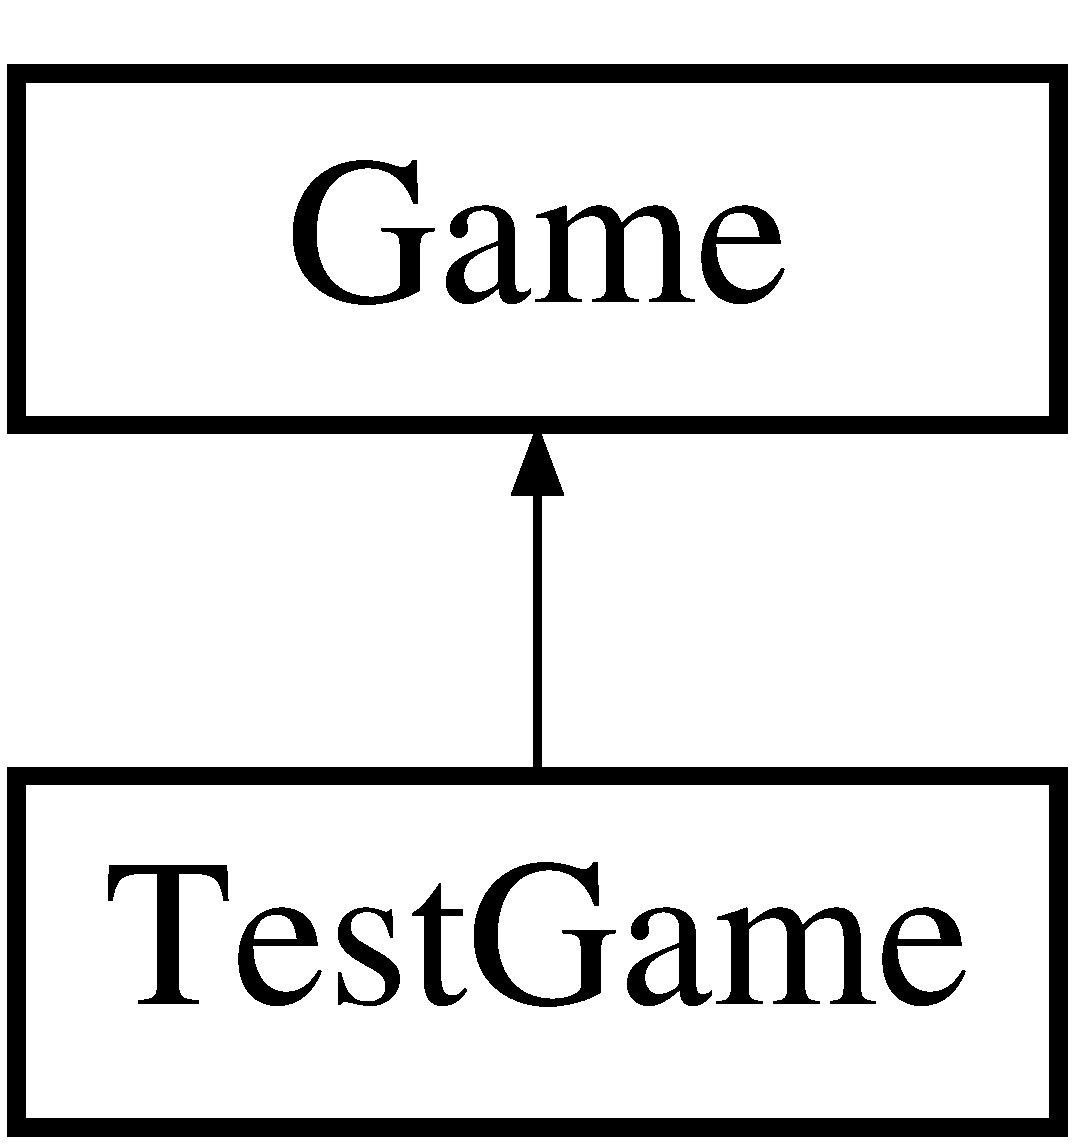
\includegraphics[height=2.000000cm]{class_test_game}
\end{center}
\end{figure}
\subsection*{Public Member Functions}
\begin{DoxyCompactItemize}
\item 
\hyperlink{class_test_game_a59adf28e5c02386f31f444e1f85aa80d}{Test\+Game} ()
\item 
virtual \hyperlink{class_test_game_ace8e119797ce64e77fc6fe317b31b35b}{$\sim$\+Test\+Game} ()
\item 
virtual void \hyperlink{class_test_game_a989e3de46c3f2b0a6ff5a3fee2741489}{Init} (const \hyperlink{class_window}{Window} \&window)
\end{DoxyCompactItemize}
\subsection*{Additional Inherited Members}


\subsection{Constructor \& Destructor Documentation}
\hypertarget{class_test_game_a59adf28e5c02386f31f444e1f85aa80d}{}\index{Test\+Game@{Test\+Game}!Test\+Game@{Test\+Game}}
\index{Test\+Game@{Test\+Game}!Test\+Game@{Test\+Game}}
\subsubsection[{Test\+Game()}]{\setlength{\rightskip}{0pt plus 5cm}Test\+Game\+::\+Test\+Game (
\begin{DoxyParamCaption}
{}
\end{DoxyParamCaption}
)\hspace{0.3cm}{\ttfamily [inline]}}\label{class_test_game_a59adf28e5c02386f31f444e1f85aa80d}
\hypertarget{class_test_game_ace8e119797ce64e77fc6fe317b31b35b}{}\index{Test\+Game@{Test\+Game}!````~Test\+Game@{$\sim$\+Test\+Game}}
\index{````~Test\+Game@{$\sim$\+Test\+Game}!Test\+Game@{Test\+Game}}
\subsubsection[{$\sim$\+Test\+Game()}]{\setlength{\rightskip}{0pt plus 5cm}virtual Test\+Game\+::$\sim$\+Test\+Game (
\begin{DoxyParamCaption}
{}
\end{DoxyParamCaption}
)\hspace{0.3cm}{\ttfamily [inline]}, {\ttfamily [virtual]}}\label{class_test_game_ace8e119797ce64e77fc6fe317b31b35b}


\subsection{Member Function Documentation}
\hypertarget{class_test_game_a989e3de46c3f2b0a6ff5a3fee2741489}{}\index{Test\+Game@{Test\+Game}!Init@{Init}}
\index{Init@{Init}!Test\+Game@{Test\+Game}}
\subsubsection[{Init(const Window \&window)}]{\setlength{\rightskip}{0pt plus 5cm}void Test\+Game\+::\+Init (
\begin{DoxyParamCaption}
\item[{const {\bf Window} \&}]{window}
\end{DoxyParamCaption}
)\hspace{0.3cm}{\ttfamily [virtual]}}\label{class_test_game_a989e3de46c3f2b0a6ff5a3fee2741489}


Reimplemented from \hyperlink{class_game_ad47d16f9908f7b9304bcd31db0717e0b}{Game}.



The documentation for this class was generated from the following file\+:\begin{DoxyCompactItemize}
\item 
F\+:/\+Fusion3\+D\+\_\+work/src/\hyperlink{main_8cpp}{main.\+cpp}\end{DoxyCompactItemize}

\hypertarget{class_test_renderer}{}\section{Test\+Renderer Class Reference}
\label{class_test_renderer}\index{Test\+Renderer@{Test\+Renderer}}
Inheritance diagram for Test\+Renderer\+:\begin{figure}[H]
\begin{center}
\leavevmode
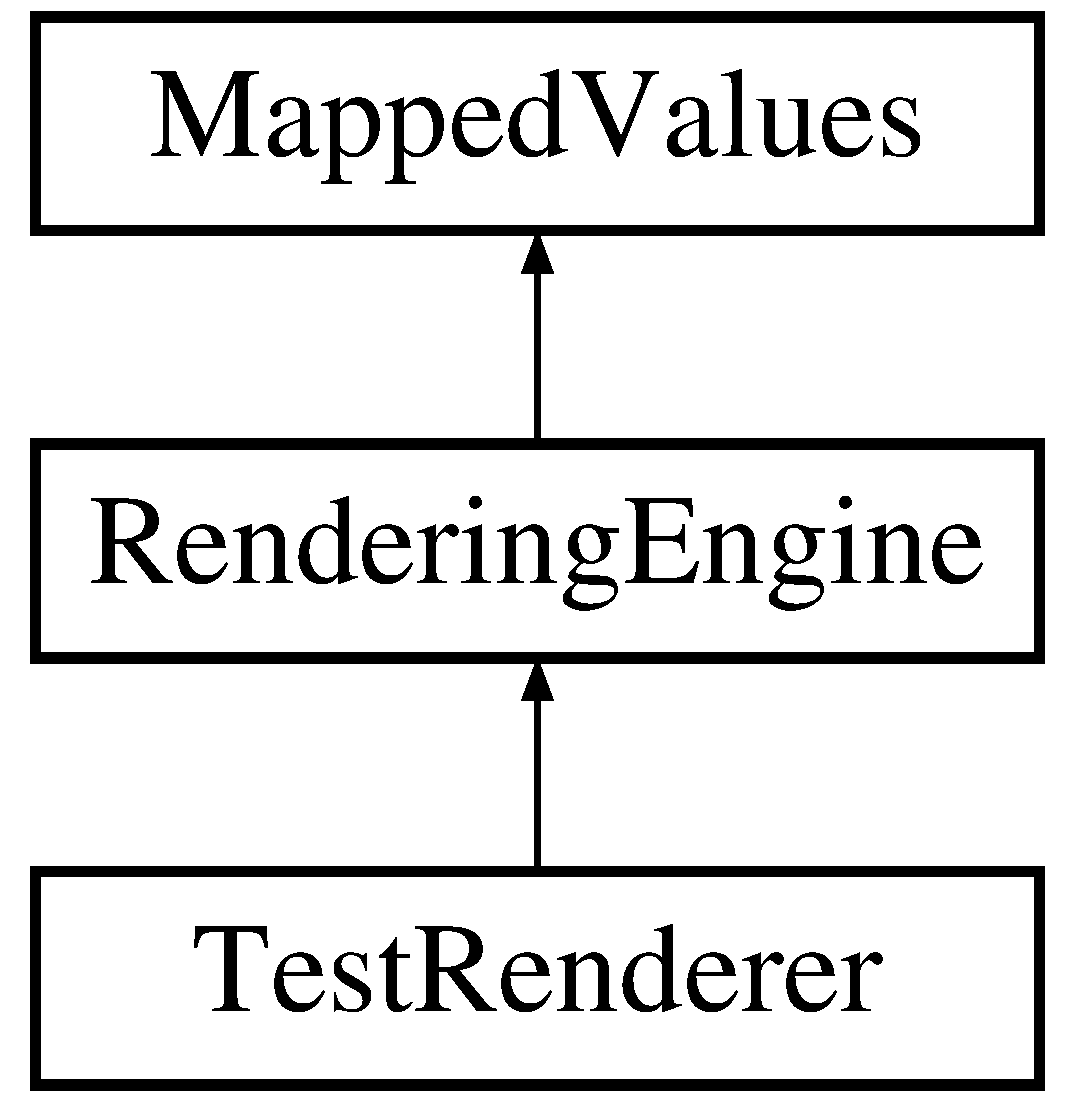
\includegraphics[height=3.000000cm]{class_test_renderer}
\end{center}
\end{figure}
\subsection*{Public Member Functions}
\begin{DoxyCompactItemize}
\item 
\hyperlink{class_test_renderer_ac5926bf8fd116f648bc945a95aac6673}{Test\+Renderer} (\hyperlink{class_window}{Window} $\ast$window)
\item 
void \hyperlink{class_test_renderer_abe86af4ad1aa4d3d68a08468ebab8f9e}{Render} (const \hyperlink{class_entity}{Entity} \&object) override
\end{DoxyCompactItemize}
\subsection*{Additional Inherited Members}


\subsection{Constructor \& Destructor Documentation}
\hypertarget{class_test_renderer_ac5926bf8fd116f648bc945a95aac6673}{}\index{Test\+Renderer@{Test\+Renderer}!Test\+Renderer@{Test\+Renderer}}
\index{Test\+Renderer@{Test\+Renderer}!Test\+Renderer@{Test\+Renderer}}
\subsubsection[{Test\+Renderer(\+Window $\ast$window)}]{\setlength{\rightskip}{0pt plus 5cm}Test\+Renderer\+::\+Test\+Renderer (
\begin{DoxyParamCaption}
\item[{{\bf Window} $\ast$}]{window}
\end{DoxyParamCaption}
)\hspace{0.3cm}{\ttfamily [inline]}}\label{class_test_renderer_ac5926bf8fd116f648bc945a95aac6673}


\subsection{Member Function Documentation}
\hypertarget{class_test_renderer_abe86af4ad1aa4d3d68a08468ebab8f9e}{}\index{Test\+Renderer@{Test\+Renderer}!Render@{Render}}
\index{Render@{Render}!Test\+Renderer@{Test\+Renderer}}
\subsubsection[{Render(const Entity \&object) override}]{\setlength{\rightskip}{0pt plus 5cm}void Test\+Renderer\+::\+Render (
\begin{DoxyParamCaption}
\item[{const {\bf Entity} \&}]{object}
\end{DoxyParamCaption}
)\hspace{0.3cm}{\ttfamily [inline]}, {\ttfamily [override]}, {\ttfamily [virtual]}}\label{class_test_renderer_abe86af4ad1aa4d3d68a08468ebab8f9e}


Reimplemented from \hyperlink{class_rendering_engine_a38ac5d7f0ed4b4933c232ca00a3adde5}{Rendering\+Engine}.



The documentation for this class was generated from the following file\+:\begin{DoxyCompactItemize}
\item 
F\+:/\+Fusion3\+D\+\_\+work/src/\hyperlink{main_8cpp}{main.\+cpp}\end{DoxyCompactItemize}

\hypertarget{class_texture}{}\section{Texture Class Reference}
\label{class_texture}\index{Texture@{Texture}}


{\ttfamily \#include $<$texture.\+h$>$}

\subsection*{Public Member Functions}
\begin{DoxyCompactItemize}
\item 
\hyperlink{class_texture_a211502d1cdd7812326479b1e72b09480}{Texture} (const std\+::string \&file\+Name, G\+Lenum texture\+Target=G\+L\+\_\+\+T\+E\+X\+T\+U\+R\+E\+\_\+2\+D, G\+Lfloat filter=G\+L\+\_\+\+L\+I\+N\+E\+A\+R\+\_\+\+M\+I\+P\+M\+A\+P\+\_\+\+L\+I\+N\+E\+A\+R, G\+Lenum internal\+Format=G\+L\+\_\+\+R\+G\+B\+A, G\+Lenum format=G\+L\+\_\+\+R\+G\+B\+A, bool clamp=false, G\+Lenum attachment=G\+L\+\_\+\+N\+O\+N\+E)
\item 
\hyperlink{class_texture_a05bec6390054493eb8780da55cc98ffb}{Texture} (int width=0, int height=0, unsigned char $\ast$data=0, G\+Lenum texture\+Target=G\+L\+\_\+\+T\+E\+X\+T\+U\+R\+E\+\_\+2\+D, G\+Lfloat filter=G\+L\+\_\+\+L\+I\+N\+E\+A\+R\+\_\+\+M\+I\+P\+M\+A\+P\+\_\+\+L\+I\+N\+E\+A\+R, G\+Lenum internal\+Format=G\+L\+\_\+\+R\+G\+B\+A, G\+Lenum format=G\+L\+\_\+\+R\+G\+B\+A, bool clamp=false, G\+Lenum attachment=G\+L\+\_\+\+N\+O\+N\+E)
\item 
\hyperlink{class_texture_a21822d3a487c6a803f706869fe46faa2}{Texture} (const \hyperlink{class_texture}{Texture} \&texture)
\item 
void \hyperlink{class_texture_ac8d4a47a87bb660ecd37b7ec7a70705b}{operator=} (\hyperlink{class_texture}{Texture} texture)
\item 
virtual \hyperlink{class_texture_a09c4bcb7462f64c1d20fa69dba3cee8a}{$\sim$\+Texture} ()
\item 
void \hyperlink{class_texture_a6f54dde94704d5f2b90c63f33c67793c}{Bind} (unsigned int unit=0) const 
\item 
void \hyperlink{class_texture_a4e8799fb199b39f37e6f2cd33891ecfd}{Bind\+As\+Render\+Target} () const 
\item 
int \hyperlink{class_texture_a1add92fc879f766aed5d39a3ef41c7cb}{Get\+Width} () const 
\item 
int \hyperlink{class_texture_adea6f153fb9fa3ac1558f4d96641e47d}{Get\+Height} () const 
\item 
bool \hyperlink{class_texture_aca3540da8292ba7dd02e6f1dbda781cc}{operator==} (const \hyperlink{class_texture}{Texture} \&texture) const 
\item 
bool \hyperlink{class_texture_abdd611487e4502e4cda4a41551bbb6f8}{operator!=} (const \hyperlink{class_texture}{Texture} \&texture) const 
\end{DoxyCompactItemize}


\subsection{Constructor \& Destructor Documentation}
\hypertarget{class_texture_a211502d1cdd7812326479b1e72b09480}{}\index{Texture@{Texture}!Texture@{Texture}}
\index{Texture@{Texture}!Texture@{Texture}}
\subsubsection[{Texture(const std\+::string \&file\+Name, G\+Lenum texture\+Target=\+G\+L\+\_\+\+T\+E\+X\+T\+U\+R\+E\+\_\+2\+D, G\+Lfloat filter=\+G\+L\+\_\+\+L\+I\+N\+E\+A\+R\+\_\+\+M\+I\+P\+M\+A\+P\+\_\+\+L\+I\+N\+E\+A\+R, G\+Lenum internal\+Format=\+G\+L\+\_\+\+R\+G\+B\+A, G\+Lenum format=\+G\+L\+\_\+\+R\+G\+B\+A, bool clamp=false, G\+Lenum attachment=\+G\+L\+\_\+\+N\+O\+N\+E)}]{\setlength{\rightskip}{0pt plus 5cm}Texture\+::\+Texture (
\begin{DoxyParamCaption}
\item[{const std\+::string \&}]{file\+Name, }
\item[{G\+Lenum}]{texture\+Target = {\ttfamily GL\+\_\+TEXTURE\+\_\+2D}, }
\item[{G\+Lfloat}]{filter = {\ttfamily GL\+\_\+LINEAR\+\_\+MIPMAP\+\_\+LINEAR}, }
\item[{G\+Lenum}]{internal\+Format = {\ttfamily GL\+\_\+RGBA}, }
\item[{G\+Lenum}]{format = {\ttfamily GL\+\_\+RGBA}, }
\item[{bool}]{clamp = {\ttfamily false}, }
\item[{G\+Lenum}]{attachment = {\ttfamily GL\+\_\+NONE}}
\end{DoxyParamCaption}
)}\label{class_texture_a211502d1cdd7812326479b1e72b09480}
\hypertarget{class_texture_a05bec6390054493eb8780da55cc98ffb}{}\index{Texture@{Texture}!Texture@{Texture}}
\index{Texture@{Texture}!Texture@{Texture}}
\subsubsection[{Texture(int width=0, int height=0, unsigned char $\ast$data=0, G\+Lenum texture\+Target=\+G\+L\+\_\+\+T\+E\+X\+T\+U\+R\+E\+\_\+2\+D, G\+Lfloat filter=\+G\+L\+\_\+\+L\+I\+N\+E\+A\+R\+\_\+\+M\+I\+P\+M\+A\+P\+\_\+\+L\+I\+N\+E\+A\+R, G\+Lenum internal\+Format=\+G\+L\+\_\+\+R\+G\+B\+A, G\+Lenum format=\+G\+L\+\_\+\+R\+G\+B\+A, bool clamp=false, G\+Lenum attachment=\+G\+L\+\_\+\+N\+O\+N\+E)}]{\setlength{\rightskip}{0pt plus 5cm}Texture\+::\+Texture (
\begin{DoxyParamCaption}
\item[{int}]{width = {\ttfamily 0}, }
\item[{int}]{height = {\ttfamily 0}, }
\item[{unsigned char $\ast$}]{data = {\ttfamily 0}, }
\item[{G\+Lenum}]{texture\+Target = {\ttfamily GL\+\_\+TEXTURE\+\_\+2D}, }
\item[{G\+Lfloat}]{filter = {\ttfamily GL\+\_\+LINEAR\+\_\+MIPMAP\+\_\+LINEAR}, }
\item[{G\+Lenum}]{internal\+Format = {\ttfamily GL\+\_\+RGBA}, }
\item[{G\+Lenum}]{format = {\ttfamily GL\+\_\+RGBA}, }
\item[{bool}]{clamp = {\ttfamily false}, }
\item[{G\+Lenum}]{attachment = {\ttfamily GL\+\_\+NONE}}
\end{DoxyParamCaption}
)}\label{class_texture_a05bec6390054493eb8780da55cc98ffb}
\hypertarget{class_texture_a21822d3a487c6a803f706869fe46faa2}{}\index{Texture@{Texture}!Texture@{Texture}}
\index{Texture@{Texture}!Texture@{Texture}}
\subsubsection[{Texture(const Texture \&texture)}]{\setlength{\rightskip}{0pt plus 5cm}Texture\+::\+Texture (
\begin{DoxyParamCaption}
\item[{const {\bf Texture} \&}]{texture}
\end{DoxyParamCaption}
)}\label{class_texture_a21822d3a487c6a803f706869fe46faa2}
\hypertarget{class_texture_a09c4bcb7462f64c1d20fa69dba3cee8a}{}\index{Texture@{Texture}!````~Texture@{$\sim$\+Texture}}
\index{````~Texture@{$\sim$\+Texture}!Texture@{Texture}}
\subsubsection[{$\sim$\+Texture()}]{\setlength{\rightskip}{0pt plus 5cm}Texture\+::$\sim$\+Texture (
\begin{DoxyParamCaption}
{}
\end{DoxyParamCaption}
)\hspace{0.3cm}{\ttfamily [virtual]}}\label{class_texture_a09c4bcb7462f64c1d20fa69dba3cee8a}


\subsection{Member Function Documentation}
\hypertarget{class_texture_a6f54dde94704d5f2b90c63f33c67793c}{}\index{Texture@{Texture}!Bind@{Bind}}
\index{Bind@{Bind}!Texture@{Texture}}
\subsubsection[{Bind(unsigned int unit=0) const }]{\setlength{\rightskip}{0pt plus 5cm}void Texture\+::\+Bind (
\begin{DoxyParamCaption}
\item[{unsigned int}]{unit = {\ttfamily 0}}
\end{DoxyParamCaption}
) const}\label{class_texture_a6f54dde94704d5f2b90c63f33c67793c}
\hypertarget{class_texture_a4e8799fb199b39f37e6f2cd33891ecfd}{}\index{Texture@{Texture}!Bind\+As\+Render\+Target@{Bind\+As\+Render\+Target}}
\index{Bind\+As\+Render\+Target@{Bind\+As\+Render\+Target}!Texture@{Texture}}
\subsubsection[{Bind\+As\+Render\+Target() const }]{\setlength{\rightskip}{0pt plus 5cm}void Texture\+::\+Bind\+As\+Render\+Target (
\begin{DoxyParamCaption}
{}
\end{DoxyParamCaption}
) const}\label{class_texture_a4e8799fb199b39f37e6f2cd33891ecfd}
\hypertarget{class_texture_adea6f153fb9fa3ac1558f4d96641e47d}{}\index{Texture@{Texture}!Get\+Height@{Get\+Height}}
\index{Get\+Height@{Get\+Height}!Texture@{Texture}}
\subsubsection[{Get\+Height() const }]{\setlength{\rightskip}{0pt plus 5cm}int Texture\+::\+Get\+Height (
\begin{DoxyParamCaption}
{}
\end{DoxyParamCaption}
) const\hspace{0.3cm}{\ttfamily [inline]}}\label{class_texture_adea6f153fb9fa3ac1558f4d96641e47d}
\hypertarget{class_texture_a1add92fc879f766aed5d39a3ef41c7cb}{}\index{Texture@{Texture}!Get\+Width@{Get\+Width}}
\index{Get\+Width@{Get\+Width}!Texture@{Texture}}
\subsubsection[{Get\+Width() const }]{\setlength{\rightskip}{0pt plus 5cm}int Texture\+::\+Get\+Width (
\begin{DoxyParamCaption}
{}
\end{DoxyParamCaption}
) const\hspace{0.3cm}{\ttfamily [inline]}}\label{class_texture_a1add92fc879f766aed5d39a3ef41c7cb}
\hypertarget{class_texture_abdd611487e4502e4cda4a41551bbb6f8}{}\index{Texture@{Texture}!operator"!=@{operator"!=}}
\index{operator"!=@{operator"!=}!Texture@{Texture}}
\subsubsection[{operator"!=(const Texture \&texture) const }]{\setlength{\rightskip}{0pt plus 5cm}bool Texture\+::operator!= (
\begin{DoxyParamCaption}
\item[{const {\bf Texture} \&}]{texture}
\end{DoxyParamCaption}
) const\hspace{0.3cm}{\ttfamily [inline]}}\label{class_texture_abdd611487e4502e4cda4a41551bbb6f8}
\hypertarget{class_texture_ac8d4a47a87bb660ecd37b7ec7a70705b}{}\index{Texture@{Texture}!operator=@{operator=}}
\index{operator=@{operator=}!Texture@{Texture}}
\subsubsection[{operator=(\+Texture texture)}]{\setlength{\rightskip}{0pt plus 5cm}void Texture\+::operator= (
\begin{DoxyParamCaption}
\item[{{\bf Texture}}]{texture}
\end{DoxyParamCaption}
)}\label{class_texture_ac8d4a47a87bb660ecd37b7ec7a70705b}
\hypertarget{class_texture_aca3540da8292ba7dd02e6f1dbda781cc}{}\index{Texture@{Texture}!operator==@{operator==}}
\index{operator==@{operator==}!Texture@{Texture}}
\subsubsection[{operator==(const Texture \&texture) const }]{\setlength{\rightskip}{0pt plus 5cm}bool Texture\+::operator== (
\begin{DoxyParamCaption}
\item[{const {\bf Texture} \&}]{texture}
\end{DoxyParamCaption}
) const\hspace{0.3cm}{\ttfamily [inline]}}\label{class_texture_aca3540da8292ba7dd02e6f1dbda781cc}


The documentation for this class was generated from the following files\+:\begin{DoxyCompactItemize}
\item 
F\+:/\+Fusion3\+D\+\_\+work/src/rendering/\hyperlink{texture_8h}{texture.\+h}\item 
F\+:/\+Fusion3\+D\+\_\+work/src/rendering/\hyperlink{texture_8cpp}{texture.\+cpp}\end{DoxyCompactItemize}

\hypertarget{class_texture_data}{}\section{Texture\+Data Class Reference}
\label{class_texture_data}\index{Texture\+Data@{Texture\+Data}}


{\ttfamily \#include $<$texture.\+h$>$}

Inheritance diagram for Texture\+Data\+:\begin{figure}[H]
\begin{center}
\leavevmode
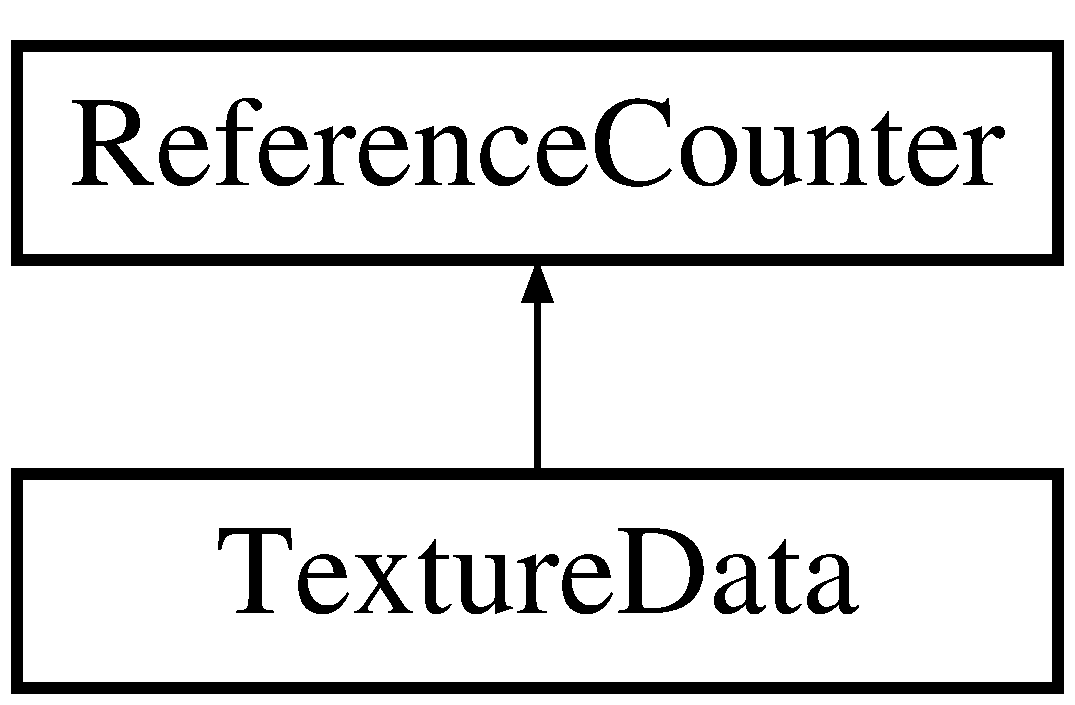
\includegraphics[height=2.000000cm]{class_texture_data}
\end{center}
\end{figure}
\subsection*{Public Member Functions}
\begin{DoxyCompactItemize}
\item 
\hyperlink{class_texture_data_ab46f64eb53b9f4dd34c936620c0f6ddb}{Texture\+Data} (G\+Lenum texture\+Target, int width, int height, int num\+Textures, unsigned char $\ast$$\ast$data, G\+Lfloat $\ast$filters, G\+Lenum $\ast$internal\+Format, G\+Lenum $\ast$format, bool clamp, G\+Lenum $\ast$attachments)
\item 
void \hyperlink{class_texture_data_aded7e6ed8e417bf39f815a671a0d84f8}{Bind} (int texture\+Num) const 
\item 
void \hyperlink{class_texture_data_a8d9a3f90f7656e1740e7ed3462f6458f}{Bind\+As\+Render\+Target} () const 
\item 
int \hyperlink{class_texture_data_ae8ddcff5940d8c244f25cf572b38d210}{Get\+Width} () const 
\item 
int \hyperlink{class_texture_data_ac812a9adc3ebb6f24a367c57aaf53f15}{Get\+Height} () const 
\item 
virtual \hyperlink{class_texture_data_ab5ba8c4b65adf5f919450fbd8374001e}{$\sim$\+Texture\+Data} ()
\end{DoxyCompactItemize}


\subsection{Constructor \& Destructor Documentation}
\hypertarget{class_texture_data_ab46f64eb53b9f4dd34c936620c0f6ddb}{}\index{Texture\+Data@{Texture\+Data}!Texture\+Data@{Texture\+Data}}
\index{Texture\+Data@{Texture\+Data}!Texture\+Data@{Texture\+Data}}
\subsubsection[{Texture\+Data(\+G\+Lenum texture\+Target, int width, int height, int num\+Textures, unsigned char $\ast$$\ast$data, G\+Lfloat $\ast$filters, G\+Lenum $\ast$internal\+Format, G\+Lenum $\ast$format, bool clamp, G\+Lenum $\ast$attachments)}]{\setlength{\rightskip}{0pt plus 5cm}Texture\+Data\+::\+Texture\+Data (
\begin{DoxyParamCaption}
\item[{G\+Lenum}]{texture\+Target, }
\item[{int}]{width, }
\item[{int}]{height, }
\item[{int}]{num\+Textures, }
\item[{unsigned char $\ast$$\ast$}]{data, }
\item[{G\+Lfloat $\ast$}]{filters, }
\item[{G\+Lenum $\ast$}]{internal\+Format, }
\item[{G\+Lenum $\ast$}]{format, }
\item[{bool}]{clamp, }
\item[{G\+Lenum $\ast$}]{attachments}
\end{DoxyParamCaption}
)}\label{class_texture_data_ab46f64eb53b9f4dd34c936620c0f6ddb}
\hypertarget{class_texture_data_ab5ba8c4b65adf5f919450fbd8374001e}{}\index{Texture\+Data@{Texture\+Data}!````~Texture\+Data@{$\sim$\+Texture\+Data}}
\index{````~Texture\+Data@{$\sim$\+Texture\+Data}!Texture\+Data@{Texture\+Data}}
\subsubsection[{$\sim$\+Texture\+Data()}]{\setlength{\rightskip}{0pt plus 5cm}Texture\+Data\+::$\sim$\+Texture\+Data (
\begin{DoxyParamCaption}
{}
\end{DoxyParamCaption}
)\hspace{0.3cm}{\ttfamily [virtual]}}\label{class_texture_data_ab5ba8c4b65adf5f919450fbd8374001e}


\subsection{Member Function Documentation}
\hypertarget{class_texture_data_aded7e6ed8e417bf39f815a671a0d84f8}{}\index{Texture\+Data@{Texture\+Data}!Bind@{Bind}}
\index{Bind@{Bind}!Texture\+Data@{Texture\+Data}}
\subsubsection[{Bind(int texture\+Num) const }]{\setlength{\rightskip}{0pt plus 5cm}void Texture\+Data\+::\+Bind (
\begin{DoxyParamCaption}
\item[{int}]{texture\+Num}
\end{DoxyParamCaption}
) const}\label{class_texture_data_aded7e6ed8e417bf39f815a671a0d84f8}
\hypertarget{class_texture_data_a8d9a3f90f7656e1740e7ed3462f6458f}{}\index{Texture\+Data@{Texture\+Data}!Bind\+As\+Render\+Target@{Bind\+As\+Render\+Target}}
\index{Bind\+As\+Render\+Target@{Bind\+As\+Render\+Target}!Texture\+Data@{Texture\+Data}}
\subsubsection[{Bind\+As\+Render\+Target() const }]{\setlength{\rightskip}{0pt plus 5cm}void Texture\+Data\+::\+Bind\+As\+Render\+Target (
\begin{DoxyParamCaption}
{}
\end{DoxyParamCaption}
) const}\label{class_texture_data_a8d9a3f90f7656e1740e7ed3462f6458f}
\hypertarget{class_texture_data_ac812a9adc3ebb6f24a367c57aaf53f15}{}\index{Texture\+Data@{Texture\+Data}!Get\+Height@{Get\+Height}}
\index{Get\+Height@{Get\+Height}!Texture\+Data@{Texture\+Data}}
\subsubsection[{Get\+Height() const }]{\setlength{\rightskip}{0pt plus 5cm}int Texture\+Data\+::\+Get\+Height (
\begin{DoxyParamCaption}
{}
\end{DoxyParamCaption}
) const\hspace{0.3cm}{\ttfamily [inline]}}\label{class_texture_data_ac812a9adc3ebb6f24a367c57aaf53f15}
\hypertarget{class_texture_data_ae8ddcff5940d8c244f25cf572b38d210}{}\index{Texture\+Data@{Texture\+Data}!Get\+Width@{Get\+Width}}
\index{Get\+Width@{Get\+Width}!Texture\+Data@{Texture\+Data}}
\subsubsection[{Get\+Width() const }]{\setlength{\rightskip}{0pt plus 5cm}int Texture\+Data\+::\+Get\+Width (
\begin{DoxyParamCaption}
{}
\end{DoxyParamCaption}
) const\hspace{0.3cm}{\ttfamily [inline]}}\label{class_texture_data_ae8ddcff5940d8c244f25cf572b38d210}


The documentation for this class was generated from the following files\+:\begin{DoxyCompactItemize}
\item 
F\+:/\+Fusion3\+D\+\_\+work/src/rendering/\hyperlink{texture_8h}{texture.\+h}\item 
F\+:/\+Fusion3\+D\+\_\+work/src/rendering/\hyperlink{texture_8cpp}{texture.\+cpp}\end{DoxyCompactItemize}

\hypertarget{class_transform}{}\section{Transform Class Reference}
\label{class_transform}\index{Transform@{Transform}}


{\ttfamily \#include $<$transform.\+h$>$}

\subsection*{Public Member Functions}
\begin{DoxyCompactItemize}
\item 
\hyperlink{class_transform_a5a7c897577867bcc5be0b0f5da5a325a}{Transform} (const \hyperlink{class_vector3f}{Vector3f} \&pos=\hyperlink{class_vector3f}{Vector3f}(0, 0, 0), const \hyperlink{class_quaternion}{Quaternion} \&rot=\hyperlink{class_quaternion}{Quaternion}(0, 0, 0, 1), float scale=1.\+0f)
\item 
\hyperlink{math3d_8h_a5b7721ab7216c91a40538beaa9e6ee1f}{Matrix4f} \hyperlink{class_transform_a11dec5b652271a3c4aebdcbc40d318c3}{Get\+Transformation} () const 
\item 
bool \hyperlink{class_transform_a2be4a2c35324d180640d3943b1aecbdd}{Has\+Changed} ()
\item 
void \hyperlink{class_transform_a3256c0fb53d0b341ad8d80fe61e5fb2d}{Update} ()
\item 
void \hyperlink{class_transform_a98a622bae4565181d7648600d9a074fc}{Rotate} (const \hyperlink{class_vector3f}{Vector3f} \&axis, float angle)
\item 
void \hyperlink{class_transform_aa44afbfad3eb5ad0506cea367ea94979}{Rotate} (const \hyperlink{class_quaternion}{Quaternion} \&rotation)
\item 
void \hyperlink{class_transform_a70a53ea2fa7600c37ab1e4929a43a193}{Look\+At} (const \hyperlink{class_vector3f}{Vector3f} \&point, const \hyperlink{class_vector3f}{Vector3f} \&up)
\item 
\hyperlink{class_quaternion}{Quaternion} \hyperlink{class_transform_a84966de18bf8e531ad377b4442f87911}{Get\+Look\+At\+Rotation} (const \hyperlink{class_vector3f}{Vector3f} \&point, const \hyperlink{class_vector3f}{Vector3f} \&up)
\item 
\hyperlink{class_vector3f}{Vector3f} $\ast$ \hyperlink{class_transform_aa4f0b5bba58b14b7357fdb975234ebaa}{Get\+Pos} ()
\item 
const \hyperlink{class_vector3f}{Vector3f} \& \hyperlink{class_transform_a6bced070570282ee5143ac7faa8c694b}{Get\+Pos} () const 
\item 
\hyperlink{class_quaternion}{Quaternion} $\ast$ \hyperlink{class_transform_a03dca2b481f971cfbf5f7b64dbe5459a}{Get\+Rot} ()
\item 
const \hyperlink{class_quaternion}{Quaternion} \& \hyperlink{class_transform_a830cca54760ecf980ebfc1ee5ac19200}{Get\+Rot} () const 
\item 
float \hyperlink{class_transform_a70d9b20871d36066d4144173044dfa5f}{Get\+Scale} () const 
\item 
\hyperlink{class_vector3f}{Vector3f} \hyperlink{class_transform_aaa07e1fe04771f89f839b325e8bfcc4c}{Get\+Transformed\+Pos} () const 
\item 
\hyperlink{class_quaternion}{Quaternion} \hyperlink{class_transform_a8bbae69612f3cd53c001d8dd00275e35}{Get\+Transformed\+Rot} () const 
\item 
bt\+Transform \hyperlink{class_transform_a91e991cd5e0e3bf4429dff1a582e2d81}{Get\+B\+T} ()
\item 
void \hyperlink{class_transform_a3a3ba4be9b592a26090dcc6d27e7bc01}{Set\+Pos} (const \hyperlink{class_vector3f}{Vector3f} \&pos)
\item 
void \hyperlink{class_transform_a859f20339cd42da87165d3146a5a922c}{Set\+Rot} (const \hyperlink{class_quaternion}{Quaternion} \&rot)
\item 
void \hyperlink{class_transform_a73296cf3be4bf21b5ac395fecd51f90c}{Set\+Scale} (float scale)
\item 
void \hyperlink{class_transform_a330267363f9085f10d1e3029b72097e7}{Set\+Parent} (\hyperlink{class_transform}{Transform} $\ast$parent)
\end{DoxyCompactItemize}
\subsection*{Static Public Member Functions}
\begin{DoxyCompactItemize}
\item 
static \hyperlink{class_transform}{Transform} \hyperlink{class_transform_a5b5ec93b4e99289c6d1a14afe7667bb7}{Get\+F\+T} (const bt\+Transform \&bt)
\end{DoxyCompactItemize}


\subsection{Constructor \& Destructor Documentation}
\hypertarget{class_transform_a5a7c897577867bcc5be0b0f5da5a325a}{}\index{Transform@{Transform}!Transform@{Transform}}
\index{Transform@{Transform}!Transform@{Transform}}
\subsubsection[{Transform(const Vector3f \&pos=\+Vector3f(0, 0, 0), const Quaternion \&rot=\+Quaternion(0, 0, 0, 1), float scale=1.\+0f)}]{\setlength{\rightskip}{0pt plus 5cm}Transform\+::\+Transform (
\begin{DoxyParamCaption}
\item[{const {\bf Vector3f} \&}]{pos = {\ttfamily {\bf Vector3f}(0,0,0)}, }
\item[{const {\bf Quaternion} \&}]{rot = {\ttfamily {\bf Quaternion}(0,0,0,1)}, }
\item[{float}]{scale = {\ttfamily 1.0f}}
\end{DoxyParamCaption}
)\hspace{0.3cm}{\ttfamily [inline]}}\label{class_transform_a5a7c897577867bcc5be0b0f5da5a325a}


\subsection{Member Function Documentation}
\hypertarget{class_transform_a91e991cd5e0e3bf4429dff1a582e2d81}{}\index{Transform@{Transform}!Get\+B\+T@{Get\+B\+T}}
\index{Get\+B\+T@{Get\+B\+T}!Transform@{Transform}}
\subsubsection[{Get\+B\+T()}]{\setlength{\rightskip}{0pt plus 5cm}bt\+Transform Transform\+::\+Get\+B\+T (
\begin{DoxyParamCaption}
{}
\end{DoxyParamCaption}
)\hspace{0.3cm}{\ttfamily [inline]}}\label{class_transform_a91e991cd5e0e3bf4429dff1a582e2d81}
\hypertarget{class_transform_a5b5ec93b4e99289c6d1a14afe7667bb7}{}\index{Transform@{Transform}!Get\+F\+T@{Get\+F\+T}}
\index{Get\+F\+T@{Get\+F\+T}!Transform@{Transform}}
\subsubsection[{Get\+F\+T(const bt\+Transform \&bt)}]{\setlength{\rightskip}{0pt plus 5cm}static {\bf Transform} Transform\+::\+Get\+F\+T (
\begin{DoxyParamCaption}
\item[{const bt\+Transform \&}]{bt}
\end{DoxyParamCaption}
)\hspace{0.3cm}{\ttfamily [inline]}, {\ttfamily [static]}}\label{class_transform_a5b5ec93b4e99289c6d1a14afe7667bb7}
\hypertarget{class_transform_a84966de18bf8e531ad377b4442f87911}{}\index{Transform@{Transform}!Get\+Look\+At\+Rotation@{Get\+Look\+At\+Rotation}}
\index{Get\+Look\+At\+Rotation@{Get\+Look\+At\+Rotation}!Transform@{Transform}}
\subsubsection[{Get\+Look\+At\+Rotation(const Vector3f \&point, const Vector3f \&up)}]{\setlength{\rightskip}{0pt plus 5cm}{\bf Quaternion} Transform\+::\+Get\+Look\+At\+Rotation (
\begin{DoxyParamCaption}
\item[{const {\bf Vector3f} \&}]{point, }
\item[{const {\bf Vector3f} \&}]{up}
\end{DoxyParamCaption}
)\hspace{0.3cm}{\ttfamily [inline]}}\label{class_transform_a84966de18bf8e531ad377b4442f87911}
\hypertarget{class_transform_aa4f0b5bba58b14b7357fdb975234ebaa}{}\index{Transform@{Transform}!Get\+Pos@{Get\+Pos}}
\index{Get\+Pos@{Get\+Pos}!Transform@{Transform}}
\subsubsection[{Get\+Pos()}]{\setlength{\rightskip}{0pt plus 5cm}{\bf Vector3f}$\ast$ Transform\+::\+Get\+Pos (
\begin{DoxyParamCaption}
{}
\end{DoxyParamCaption}
)\hspace{0.3cm}{\ttfamily [inline]}}\label{class_transform_aa4f0b5bba58b14b7357fdb975234ebaa}
\hypertarget{class_transform_a6bced070570282ee5143ac7faa8c694b}{}\index{Transform@{Transform}!Get\+Pos@{Get\+Pos}}
\index{Get\+Pos@{Get\+Pos}!Transform@{Transform}}
\subsubsection[{Get\+Pos() const }]{\setlength{\rightskip}{0pt plus 5cm}const {\bf Vector3f}\& Transform\+::\+Get\+Pos (
\begin{DoxyParamCaption}
{}
\end{DoxyParamCaption}
) const\hspace{0.3cm}{\ttfamily [inline]}}\label{class_transform_a6bced070570282ee5143ac7faa8c694b}
\hypertarget{class_transform_a03dca2b481f971cfbf5f7b64dbe5459a}{}\index{Transform@{Transform}!Get\+Rot@{Get\+Rot}}
\index{Get\+Rot@{Get\+Rot}!Transform@{Transform}}
\subsubsection[{Get\+Rot()}]{\setlength{\rightskip}{0pt plus 5cm}{\bf Quaternion}$\ast$ Transform\+::\+Get\+Rot (
\begin{DoxyParamCaption}
{}
\end{DoxyParamCaption}
)\hspace{0.3cm}{\ttfamily [inline]}}\label{class_transform_a03dca2b481f971cfbf5f7b64dbe5459a}
\hypertarget{class_transform_a830cca54760ecf980ebfc1ee5ac19200}{}\index{Transform@{Transform}!Get\+Rot@{Get\+Rot}}
\index{Get\+Rot@{Get\+Rot}!Transform@{Transform}}
\subsubsection[{Get\+Rot() const }]{\setlength{\rightskip}{0pt plus 5cm}const {\bf Quaternion}\& Transform\+::\+Get\+Rot (
\begin{DoxyParamCaption}
{}
\end{DoxyParamCaption}
) const\hspace{0.3cm}{\ttfamily [inline]}}\label{class_transform_a830cca54760ecf980ebfc1ee5ac19200}
\hypertarget{class_transform_a70d9b20871d36066d4144173044dfa5f}{}\index{Transform@{Transform}!Get\+Scale@{Get\+Scale}}
\index{Get\+Scale@{Get\+Scale}!Transform@{Transform}}
\subsubsection[{Get\+Scale() const }]{\setlength{\rightskip}{0pt plus 5cm}float Transform\+::\+Get\+Scale (
\begin{DoxyParamCaption}
{}
\end{DoxyParamCaption}
) const\hspace{0.3cm}{\ttfamily [inline]}}\label{class_transform_a70d9b20871d36066d4144173044dfa5f}
\hypertarget{class_transform_a11dec5b652271a3c4aebdcbc40d318c3}{}\index{Transform@{Transform}!Get\+Transformation@{Get\+Transformation}}
\index{Get\+Transformation@{Get\+Transformation}!Transform@{Transform}}
\subsubsection[{Get\+Transformation() const }]{\setlength{\rightskip}{0pt plus 5cm}{\bf Matrix4f} Transform\+::\+Get\+Transformation (
\begin{DoxyParamCaption}
{}
\end{DoxyParamCaption}
) const}\label{class_transform_a11dec5b652271a3c4aebdcbc40d318c3}
\hypertarget{class_transform_aaa07e1fe04771f89f839b325e8bfcc4c}{}\index{Transform@{Transform}!Get\+Transformed\+Pos@{Get\+Transformed\+Pos}}
\index{Get\+Transformed\+Pos@{Get\+Transformed\+Pos}!Transform@{Transform}}
\subsubsection[{Get\+Transformed\+Pos() const }]{\setlength{\rightskip}{0pt plus 5cm}{\bf Vector3f} Transform\+::\+Get\+Transformed\+Pos (
\begin{DoxyParamCaption}
{}
\end{DoxyParamCaption}
) const\hspace{0.3cm}{\ttfamily [inline]}}\label{class_transform_aaa07e1fe04771f89f839b325e8bfcc4c}
\hypertarget{class_transform_a8bbae69612f3cd53c001d8dd00275e35}{}\index{Transform@{Transform}!Get\+Transformed\+Rot@{Get\+Transformed\+Rot}}
\index{Get\+Transformed\+Rot@{Get\+Transformed\+Rot}!Transform@{Transform}}
\subsubsection[{Get\+Transformed\+Rot() const }]{\setlength{\rightskip}{0pt plus 5cm}{\bf Quaternion} Transform\+::\+Get\+Transformed\+Rot (
\begin{DoxyParamCaption}
{}
\end{DoxyParamCaption}
) const}\label{class_transform_a8bbae69612f3cd53c001d8dd00275e35}
\hypertarget{class_transform_a2be4a2c35324d180640d3943b1aecbdd}{}\index{Transform@{Transform}!Has\+Changed@{Has\+Changed}}
\index{Has\+Changed@{Has\+Changed}!Transform@{Transform}}
\subsubsection[{Has\+Changed()}]{\setlength{\rightskip}{0pt plus 5cm}bool Transform\+::\+Has\+Changed (
\begin{DoxyParamCaption}
{}
\end{DoxyParamCaption}
)}\label{class_transform_a2be4a2c35324d180640d3943b1aecbdd}
\hypertarget{class_transform_a70a53ea2fa7600c37ab1e4929a43a193}{}\index{Transform@{Transform}!Look\+At@{Look\+At}}
\index{Look\+At@{Look\+At}!Transform@{Transform}}
\subsubsection[{Look\+At(const Vector3f \&point, const Vector3f \&up)}]{\setlength{\rightskip}{0pt plus 5cm}void Transform\+::\+Look\+At (
\begin{DoxyParamCaption}
\item[{const {\bf Vector3f} \&}]{point, }
\item[{const {\bf Vector3f} \&}]{up}
\end{DoxyParamCaption}
)}\label{class_transform_a70a53ea2fa7600c37ab1e4929a43a193}
\hypertarget{class_transform_a98a622bae4565181d7648600d9a074fc}{}\index{Transform@{Transform}!Rotate@{Rotate}}
\index{Rotate@{Rotate}!Transform@{Transform}}
\subsubsection[{Rotate(const Vector3f \&axis, float angle)}]{\setlength{\rightskip}{0pt plus 5cm}void Transform\+::\+Rotate (
\begin{DoxyParamCaption}
\item[{const {\bf Vector3f} \&}]{axis, }
\item[{float}]{angle}
\end{DoxyParamCaption}
)}\label{class_transform_a98a622bae4565181d7648600d9a074fc}
\hypertarget{class_transform_aa44afbfad3eb5ad0506cea367ea94979}{}\index{Transform@{Transform}!Rotate@{Rotate}}
\index{Rotate@{Rotate}!Transform@{Transform}}
\subsubsection[{Rotate(const Quaternion \&rotation)}]{\setlength{\rightskip}{0pt plus 5cm}void Transform\+::\+Rotate (
\begin{DoxyParamCaption}
\item[{const {\bf Quaternion} \&}]{rotation}
\end{DoxyParamCaption}
)}\label{class_transform_aa44afbfad3eb5ad0506cea367ea94979}
\hypertarget{class_transform_a330267363f9085f10d1e3029b72097e7}{}\index{Transform@{Transform}!Set\+Parent@{Set\+Parent}}
\index{Set\+Parent@{Set\+Parent}!Transform@{Transform}}
\subsubsection[{Set\+Parent(\+Transform $\ast$parent)}]{\setlength{\rightskip}{0pt plus 5cm}void Transform\+::\+Set\+Parent (
\begin{DoxyParamCaption}
\item[{{\bf Transform} $\ast$}]{parent}
\end{DoxyParamCaption}
)\hspace{0.3cm}{\ttfamily [inline]}}\label{class_transform_a330267363f9085f10d1e3029b72097e7}
\hypertarget{class_transform_a3a3ba4be9b592a26090dcc6d27e7bc01}{}\index{Transform@{Transform}!Set\+Pos@{Set\+Pos}}
\index{Set\+Pos@{Set\+Pos}!Transform@{Transform}}
\subsubsection[{Set\+Pos(const Vector3f \&pos)}]{\setlength{\rightskip}{0pt plus 5cm}void Transform\+::\+Set\+Pos (
\begin{DoxyParamCaption}
\item[{const {\bf Vector3f} \&}]{pos}
\end{DoxyParamCaption}
)\hspace{0.3cm}{\ttfamily [inline]}}\label{class_transform_a3a3ba4be9b592a26090dcc6d27e7bc01}
\hypertarget{class_transform_a859f20339cd42da87165d3146a5a922c}{}\index{Transform@{Transform}!Set\+Rot@{Set\+Rot}}
\index{Set\+Rot@{Set\+Rot}!Transform@{Transform}}
\subsubsection[{Set\+Rot(const Quaternion \&rot)}]{\setlength{\rightskip}{0pt plus 5cm}void Transform\+::\+Set\+Rot (
\begin{DoxyParamCaption}
\item[{const {\bf Quaternion} \&}]{rot}
\end{DoxyParamCaption}
)\hspace{0.3cm}{\ttfamily [inline]}}\label{class_transform_a859f20339cd42da87165d3146a5a922c}
\hypertarget{class_transform_a73296cf3be4bf21b5ac395fecd51f90c}{}\index{Transform@{Transform}!Set\+Scale@{Set\+Scale}}
\index{Set\+Scale@{Set\+Scale}!Transform@{Transform}}
\subsubsection[{Set\+Scale(float scale)}]{\setlength{\rightskip}{0pt plus 5cm}void Transform\+::\+Set\+Scale (
\begin{DoxyParamCaption}
\item[{float}]{scale}
\end{DoxyParamCaption}
)\hspace{0.3cm}{\ttfamily [inline]}}\label{class_transform_a73296cf3be4bf21b5ac395fecd51f90c}
\hypertarget{class_transform_a3256c0fb53d0b341ad8d80fe61e5fb2d}{}\index{Transform@{Transform}!Update@{Update}}
\index{Update@{Update}!Transform@{Transform}}
\subsubsection[{Update()}]{\setlength{\rightskip}{0pt plus 5cm}void Transform\+::\+Update (
\begin{DoxyParamCaption}
{}
\end{DoxyParamCaption}
)}\label{class_transform_a3256c0fb53d0b341ad8d80fe61e5fb2d}


The documentation for this class was generated from the following files\+:\begin{DoxyCompactItemize}
\item 
F\+:/\+Fusion3\+D\+\_\+work/src/core/\hyperlink{transform_8h}{transform.\+h}\item 
F\+:/\+Fusion3\+D\+\_\+work/src/core/\hyperlink{transform_8cpp}{transform.\+cpp}\end{DoxyCompactItemize}

\hypertarget{class_typed_data}{}\section{Typed\+Data Class Reference}
\label{class_typed_data}\index{Typed\+Data@{Typed\+Data}}


{\ttfamily \#include $<$shader.\+h$>$}

\subsection*{Public Member Functions}
\begin{DoxyCompactItemize}
\item 
\hyperlink{class_typed_data_a75648dfe5f728a060c644b42510734e1}{Typed\+Data} (const std\+::string \&name, const std\+::string \&type)
\item 
const std\+::string \& \hyperlink{class_typed_data_a6493a7e9b4ca01b2a3ce5e6dc13dfc49}{Get\+Name} () const 
\item 
const std\+::string \& \hyperlink{class_typed_data_af856e7cf10bec8a5bc608b41f2a4c0b6}{Get\+Type} () const 
\end{DoxyCompactItemize}


\subsection{Constructor \& Destructor Documentation}
\hypertarget{class_typed_data_a75648dfe5f728a060c644b42510734e1}{}\index{Typed\+Data@{Typed\+Data}!Typed\+Data@{Typed\+Data}}
\index{Typed\+Data@{Typed\+Data}!Typed\+Data@{Typed\+Data}}
\subsubsection[{Typed\+Data(const std\+::string \&name, const std\+::string \&type)}]{\setlength{\rightskip}{0pt plus 5cm}Typed\+Data\+::\+Typed\+Data (
\begin{DoxyParamCaption}
\item[{const std\+::string \&}]{name, }
\item[{const std\+::string \&}]{type}
\end{DoxyParamCaption}
)\hspace{0.3cm}{\ttfamily [inline]}}\label{class_typed_data_a75648dfe5f728a060c644b42510734e1}


\subsection{Member Function Documentation}
\hypertarget{class_typed_data_a6493a7e9b4ca01b2a3ce5e6dc13dfc49}{}\index{Typed\+Data@{Typed\+Data}!Get\+Name@{Get\+Name}}
\index{Get\+Name@{Get\+Name}!Typed\+Data@{Typed\+Data}}
\subsubsection[{Get\+Name() const }]{\setlength{\rightskip}{0pt plus 5cm}const std\+::string\& Typed\+Data\+::\+Get\+Name (
\begin{DoxyParamCaption}
{}
\end{DoxyParamCaption}
) const\hspace{0.3cm}{\ttfamily [inline]}}\label{class_typed_data_a6493a7e9b4ca01b2a3ce5e6dc13dfc49}
\hypertarget{class_typed_data_af856e7cf10bec8a5bc608b41f2a4c0b6}{}\index{Typed\+Data@{Typed\+Data}!Get\+Type@{Get\+Type}}
\index{Get\+Type@{Get\+Type}!Typed\+Data@{Typed\+Data}}
\subsubsection[{Get\+Type() const }]{\setlength{\rightskip}{0pt plus 5cm}const std\+::string\& Typed\+Data\+::\+Get\+Type (
\begin{DoxyParamCaption}
{}
\end{DoxyParamCaption}
) const\hspace{0.3cm}{\ttfamily [inline]}}\label{class_typed_data_af856e7cf10bec8a5bc608b41f2a4c0b6}


The documentation for this class was generated from the following file\+:\begin{DoxyCompactItemize}
\item 
F\+:/\+Fusion3\+D\+\_\+work/src/rendering/\hyperlink{shader_8h}{shader.\+h}\end{DoxyCompactItemize}

\hypertarget{class_uniform_struct}{}\section{Uniform\+Struct Class Reference}
\label{class_uniform_struct}\index{Uniform\+Struct@{Uniform\+Struct}}


{\ttfamily \#include $<$shader.\+h$>$}

\subsection*{Public Member Functions}
\begin{DoxyCompactItemize}
\item 
\hyperlink{class_uniform_struct_adf5073a80c5be9bcdb3a32642fb033d3}{Uniform\+Struct} (const std\+::string \&name, const std\+::vector$<$ \hyperlink{class_typed_data}{Typed\+Data} $>$ \&member\+Names)
\item 
const std\+::string \& \hyperlink{class_uniform_struct_aba4c840bffbd67897443906baa91e113}{Get\+Name} () const 
\item 
const std\+::vector$<$ \hyperlink{class_typed_data}{Typed\+Data} $>$ \& \hyperlink{class_uniform_struct_a3cfea35a3fdc46fa4616a47be677fdd3}{Get\+Member\+Names} () const 
\end{DoxyCompactItemize}


\subsection{Constructor \& Destructor Documentation}
\hypertarget{class_uniform_struct_adf5073a80c5be9bcdb3a32642fb033d3}{}\index{Uniform\+Struct@{Uniform\+Struct}!Uniform\+Struct@{Uniform\+Struct}}
\index{Uniform\+Struct@{Uniform\+Struct}!Uniform\+Struct@{Uniform\+Struct}}
\subsubsection[{Uniform\+Struct(const std\+::string \&name, const std\+::vector$<$ Typed\+Data $>$ \&member\+Names)}]{\setlength{\rightskip}{0pt plus 5cm}Uniform\+Struct\+::\+Uniform\+Struct (
\begin{DoxyParamCaption}
\item[{const std\+::string \&}]{name, }
\item[{const std\+::vector$<$ {\bf Typed\+Data} $>$ \&}]{member\+Names}
\end{DoxyParamCaption}
)\hspace{0.3cm}{\ttfamily [inline]}}\label{class_uniform_struct_adf5073a80c5be9bcdb3a32642fb033d3}


\subsection{Member Function Documentation}
\hypertarget{class_uniform_struct_a3cfea35a3fdc46fa4616a47be677fdd3}{}\index{Uniform\+Struct@{Uniform\+Struct}!Get\+Member\+Names@{Get\+Member\+Names}}
\index{Get\+Member\+Names@{Get\+Member\+Names}!Uniform\+Struct@{Uniform\+Struct}}
\subsubsection[{Get\+Member\+Names() const }]{\setlength{\rightskip}{0pt plus 5cm}const std\+::vector$<${\bf Typed\+Data}$>$\& Uniform\+Struct\+::\+Get\+Member\+Names (
\begin{DoxyParamCaption}
{}
\end{DoxyParamCaption}
) const\hspace{0.3cm}{\ttfamily [inline]}}\label{class_uniform_struct_a3cfea35a3fdc46fa4616a47be677fdd3}
\hypertarget{class_uniform_struct_aba4c840bffbd67897443906baa91e113}{}\index{Uniform\+Struct@{Uniform\+Struct}!Get\+Name@{Get\+Name}}
\index{Get\+Name@{Get\+Name}!Uniform\+Struct@{Uniform\+Struct}}
\subsubsection[{Get\+Name() const }]{\setlength{\rightskip}{0pt plus 5cm}const std\+::string\& Uniform\+Struct\+::\+Get\+Name (
\begin{DoxyParamCaption}
{}
\end{DoxyParamCaption}
) const\hspace{0.3cm}{\ttfamily [inline]}}\label{class_uniform_struct_aba4c840bffbd67897443906baa91e113}


The documentation for this class was generated from the following file\+:\begin{DoxyCompactItemize}
\item 
F\+:/\+Fusion3\+D\+\_\+work/src/rendering/\hyperlink{shader_8h}{shader.\+h}\end{DoxyCompactItemize}

\hypertarget{class_vector}{}\section{Vector$<$ T, D $>$ Class Template Reference}
\label{class_vector}\index{Vector$<$ T, D $>$@{Vector$<$ T, D $>$}}


{\ttfamily \#include $<$math3d.\+h$>$}

\subsection*{Public Member Functions}
\begin{DoxyCompactItemize}
\item 
\hyperlink{class_vector_a3c785a9866bb20fc79b19196fe9b3a5b}{Vector} ()
\item 
T \hyperlink{class_vector_a70c3348b3fcab9e06f120b8e7a9b0a40}{Dot} (const \hyperlink{class_vector}{Vector}$<$ T, D $>$ \&r) const 
\item 
\hyperlink{class_vector}{Vector}$<$ T, D $>$ \hyperlink{class_vector_adb18e41faad27d9cef7a4629b6fe53b9}{Max} (const \hyperlink{class_vector}{Vector}$<$ T, D $>$ \&r) const 
\item 
T \hyperlink{class_vector_a428af4a05c03660f55cddb78696c2d38}{Max} () const 
\item 
T \hyperlink{class_vector_a197762230f85ba8e0ce7460dfa0000df}{Length\+Sq} () const 
\item 
T \hyperlink{class_vector_a68702092267c728db02f67c518c9583f}{Length} () const 
\item 
\hyperlink{class_vector}{Vector}$<$ T, D $>$ \hyperlink{class_vector_a42dc6fba30ea0f61e3dbf1031876d539}{Normalized} () const 
\item 
\hyperlink{class_vector}{Vector}$<$ T, D $>$ \hyperlink{class_vector_aa78265179b17460e314b8931f498974c}{Lerp} (const \hyperlink{class_vector}{Vector}$<$ T, D $>$ \&r, T lerp\+Factor) const 
\item 
\hyperlink{class_vector}{Vector}$<$ T, D $>$ \hyperlink{class_vector_a4a4933d141bf4bf006f12738538fa0c9}{Reflect} (const \hyperlink{class_vector}{Vector}$<$ T, D $>$ \&normal) const 
\item 
\hyperlink{class_vector}{Vector}$<$ T, D $>$ \hyperlink{class_vector_a26e7de8248521c9c943901ab197e0382}{operator+} (const \hyperlink{class_vector}{Vector}$<$ T, D $>$ \&r) const 
\item 
\hyperlink{class_vector}{Vector}$<$ T, D $>$ \hyperlink{class_vector_af24d7aceedbf168d05e692d88d46fae1}{operator-\/} (const \hyperlink{class_vector}{Vector}$<$ T, D $>$ \&r) const 
\item 
\hyperlink{class_vector}{Vector}$<$ T, D $>$ \hyperlink{class_vector_a954ad102eae0acb0eeca7b9cc1e5a4fe}{operator$\ast$} (const T \&r) const 
\item 
\hyperlink{class_vector}{Vector}$<$ T, D $>$ \hyperlink{class_vector_aaee4aa213a1cc7d8994654dd97f19b18}{operator/} (const T \&r) const 
\item 
\hyperlink{class_vector}{Vector}$<$ T, D $>$ \& \hyperlink{class_vector_ae1fa7e41ff5a0203a2cca31a490c3938}{operator+=} (const \hyperlink{class_vector}{Vector}$<$ T, D $>$ \&r)
\item 
\hyperlink{class_vector}{Vector}$<$ T, D $>$ \& \hyperlink{class_vector_a4b8dacc089cf007bd03df1d0c7850a45}{operator-\/=} (const \hyperlink{class_vector}{Vector}$<$ T, D $>$ \&r)
\item 
\hyperlink{class_vector}{Vector}$<$ T, D $>$ \& \hyperlink{class_vector_a707fb8da27e69f86c8f159b2bedd77f2}{operator$\ast$=} (const T \&r)
\item 
\hyperlink{class_vector}{Vector}$<$ T, D $>$ \& \hyperlink{class_vector_a0903cfeaa393ae932f42db553e41565d}{operator/=} (const T \&r)
\item 
T \& \hyperlink{class_vector_a8f0c8fbf73a5863e3cb73908876490c1}{operator\mbox{[}$\,$\mbox{]}} (unsigned int i)
\item 
T \hyperlink{class_vector_a31a62f16c97ea15a32944549b61027ef}{operator\mbox{[}$\,$\mbox{]}} (unsigned int i) const 
\item 
bool \hyperlink{class_vector_a62b7ae1dc75c2f8cb365e1927a6d2ed0}{operator==} (const \hyperlink{class_vector}{Vector}$<$ T, D $>$ \&r) const 
\item 
bool \hyperlink{class_vector_a5cf05408812e111be67d7625aee50834}{operator!=} (const \hyperlink{class_vector}{Vector}$<$ T, D $>$ \&r) const 
\end{DoxyCompactItemize}


\subsection{Constructor \& Destructor Documentation}
\hypertarget{class_vector_a3c785a9866bb20fc79b19196fe9b3a5b}{}\index{Vector@{Vector}!Vector@{Vector}}
\index{Vector@{Vector}!Vector@{Vector}}
\subsubsection[{Vector()}]{\setlength{\rightskip}{0pt plus 5cm}template$<$typename T, unsigned int D$>$ {\bf Vector}$<$ T, D $>$\+::{\bf Vector} (
\begin{DoxyParamCaption}
{}
\end{DoxyParamCaption}
)\hspace{0.3cm}{\ttfamily [inline]}}\label{class_vector_a3c785a9866bb20fc79b19196fe9b3a5b}


\subsection{Member Function Documentation}
\hypertarget{class_vector_a70c3348b3fcab9e06f120b8e7a9b0a40}{}\index{Vector@{Vector}!Dot@{Dot}}
\index{Dot@{Dot}!Vector@{Vector}}
\subsubsection[{Dot(const Vector$<$ T, D $>$ \&r) const }]{\setlength{\rightskip}{0pt plus 5cm}template$<$typename T, unsigned int D$>$ T {\bf Vector}$<$ T, D $>$\+::Dot (
\begin{DoxyParamCaption}
\item[{const {\bf Vector}$<$ T, D $>$ \&}]{r}
\end{DoxyParamCaption}
) const\hspace{0.3cm}{\ttfamily [inline]}}\label{class_vector_a70c3348b3fcab9e06f120b8e7a9b0a40}
\hypertarget{class_vector_a68702092267c728db02f67c518c9583f}{}\index{Vector@{Vector}!Length@{Length}}
\index{Length@{Length}!Vector@{Vector}}
\subsubsection[{Length() const }]{\setlength{\rightskip}{0pt plus 5cm}template$<$typename T, unsigned int D$>$ T {\bf Vector}$<$ T, D $>$\+::Length (
\begin{DoxyParamCaption}
{}
\end{DoxyParamCaption}
) const\hspace{0.3cm}{\ttfamily [inline]}}\label{class_vector_a68702092267c728db02f67c518c9583f}
\hypertarget{class_vector_a197762230f85ba8e0ce7460dfa0000df}{}\index{Vector@{Vector}!Length\+Sq@{Length\+Sq}}
\index{Length\+Sq@{Length\+Sq}!Vector@{Vector}}
\subsubsection[{Length\+Sq() const }]{\setlength{\rightskip}{0pt plus 5cm}template$<$typename T, unsigned int D$>$ T {\bf Vector}$<$ T, D $>$\+::Length\+Sq (
\begin{DoxyParamCaption}
{}
\end{DoxyParamCaption}
) const\hspace{0.3cm}{\ttfamily [inline]}}\label{class_vector_a197762230f85ba8e0ce7460dfa0000df}
\hypertarget{class_vector_aa78265179b17460e314b8931f498974c}{}\index{Vector@{Vector}!Lerp@{Lerp}}
\index{Lerp@{Lerp}!Vector@{Vector}}
\subsubsection[{Lerp(const Vector$<$ T, D $>$ \&r, T lerp\+Factor) const }]{\setlength{\rightskip}{0pt plus 5cm}template$<$typename T, unsigned int D$>$ {\bf Vector}$<$T,D$>$ {\bf Vector}$<$ T, D $>$\+::Lerp (
\begin{DoxyParamCaption}
\item[{const {\bf Vector}$<$ T, D $>$ \&}]{r, }
\item[{T}]{lerp\+Factor}
\end{DoxyParamCaption}
) const\hspace{0.3cm}{\ttfamily [inline]}}\label{class_vector_aa78265179b17460e314b8931f498974c}
\hypertarget{class_vector_adb18e41faad27d9cef7a4629b6fe53b9}{}\index{Vector@{Vector}!Max@{Max}}
\index{Max@{Max}!Vector@{Vector}}
\subsubsection[{Max(const Vector$<$ T, D $>$ \&r) const }]{\setlength{\rightskip}{0pt plus 5cm}template$<$typename T, unsigned int D$>$ {\bf Vector}$<$T,D$>$ {\bf Vector}$<$ T, D $>$\+::Max (
\begin{DoxyParamCaption}
\item[{const {\bf Vector}$<$ T, D $>$ \&}]{r}
\end{DoxyParamCaption}
) const\hspace{0.3cm}{\ttfamily [inline]}}\label{class_vector_adb18e41faad27d9cef7a4629b6fe53b9}
\hypertarget{class_vector_a428af4a05c03660f55cddb78696c2d38}{}\index{Vector@{Vector}!Max@{Max}}
\index{Max@{Max}!Vector@{Vector}}
\subsubsection[{Max() const }]{\setlength{\rightskip}{0pt plus 5cm}template$<$typename T, unsigned int D$>$ T {\bf Vector}$<$ T, D $>$\+::Max (
\begin{DoxyParamCaption}
{}
\end{DoxyParamCaption}
) const\hspace{0.3cm}{\ttfamily [inline]}}\label{class_vector_a428af4a05c03660f55cddb78696c2d38}
\hypertarget{class_vector_a42dc6fba30ea0f61e3dbf1031876d539}{}\index{Vector@{Vector}!Normalized@{Normalized}}
\index{Normalized@{Normalized}!Vector@{Vector}}
\subsubsection[{Normalized() const }]{\setlength{\rightskip}{0pt plus 5cm}template$<$typename T, unsigned int D$>$ {\bf Vector}$<$T,D$>$ {\bf Vector}$<$ T, D $>$\+::Normalized (
\begin{DoxyParamCaption}
{}
\end{DoxyParamCaption}
) const\hspace{0.3cm}{\ttfamily [inline]}}\label{class_vector_a42dc6fba30ea0f61e3dbf1031876d539}
\hypertarget{class_vector_a5cf05408812e111be67d7625aee50834}{}\index{Vector@{Vector}!operator"!=@{operator"!=}}
\index{operator"!=@{operator"!=}!Vector@{Vector}}
\subsubsection[{operator"!=(const Vector$<$ T, D $>$ \&r) const }]{\setlength{\rightskip}{0pt plus 5cm}template$<$typename T, unsigned int D$>$ bool {\bf Vector}$<$ T, D $>$\+::operator!= (
\begin{DoxyParamCaption}
\item[{const {\bf Vector}$<$ T, D $>$ \&}]{r}
\end{DoxyParamCaption}
) const\hspace{0.3cm}{\ttfamily [inline]}}\label{class_vector_a5cf05408812e111be67d7625aee50834}
\hypertarget{class_vector_a954ad102eae0acb0eeca7b9cc1e5a4fe}{}\index{Vector@{Vector}!operator$\ast$@{operator$\ast$}}
\index{operator$\ast$@{operator$\ast$}!Vector@{Vector}}
\subsubsection[{operator$\ast$(const T \&r) const }]{\setlength{\rightskip}{0pt plus 5cm}template$<$typename T, unsigned int D$>$ {\bf Vector}$<$T, D$>$ {\bf Vector}$<$ T, D $>$\+::operator$\ast$ (
\begin{DoxyParamCaption}
\item[{const T \&}]{r}
\end{DoxyParamCaption}
) const\hspace{0.3cm}{\ttfamily [inline]}}\label{class_vector_a954ad102eae0acb0eeca7b9cc1e5a4fe}
\hypertarget{class_vector_a707fb8da27e69f86c8f159b2bedd77f2}{}\index{Vector@{Vector}!operator$\ast$=@{operator$\ast$=}}
\index{operator$\ast$=@{operator$\ast$=}!Vector@{Vector}}
\subsubsection[{operator$\ast$=(const T \&r)}]{\setlength{\rightskip}{0pt plus 5cm}template$<$typename T, unsigned int D$>$ {\bf Vector}$<$T, D$>$\& {\bf Vector}$<$ T, D $>$\+::operator$\ast$= (
\begin{DoxyParamCaption}
\item[{const T \&}]{r}
\end{DoxyParamCaption}
)\hspace{0.3cm}{\ttfamily [inline]}}\label{class_vector_a707fb8da27e69f86c8f159b2bedd77f2}
\hypertarget{class_vector_a26e7de8248521c9c943901ab197e0382}{}\index{Vector@{Vector}!operator+@{operator+}}
\index{operator+@{operator+}!Vector@{Vector}}
\subsubsection[{operator+(const Vector$<$ T, D $>$ \&r) const }]{\setlength{\rightskip}{0pt plus 5cm}template$<$typename T, unsigned int D$>$ {\bf Vector}$<$T, D$>$ {\bf Vector}$<$ T, D $>$\+::operator+ (
\begin{DoxyParamCaption}
\item[{const {\bf Vector}$<$ T, D $>$ \&}]{r}
\end{DoxyParamCaption}
) const\hspace{0.3cm}{\ttfamily [inline]}}\label{class_vector_a26e7de8248521c9c943901ab197e0382}
\hypertarget{class_vector_ae1fa7e41ff5a0203a2cca31a490c3938}{}\index{Vector@{Vector}!operator+=@{operator+=}}
\index{operator+=@{operator+=}!Vector@{Vector}}
\subsubsection[{operator+=(const Vector$<$ T, D $>$ \&r)}]{\setlength{\rightskip}{0pt plus 5cm}template$<$typename T, unsigned int D$>$ {\bf Vector}$<$T, D$>$\& {\bf Vector}$<$ T, D $>$\+::operator+= (
\begin{DoxyParamCaption}
\item[{const {\bf Vector}$<$ T, D $>$ \&}]{r}
\end{DoxyParamCaption}
)\hspace{0.3cm}{\ttfamily [inline]}}\label{class_vector_ae1fa7e41ff5a0203a2cca31a490c3938}
\hypertarget{class_vector_af24d7aceedbf168d05e692d88d46fae1}{}\index{Vector@{Vector}!operator-\/@{operator-\/}}
\index{operator-\/@{operator-\/}!Vector@{Vector}}
\subsubsection[{operator-\/(const Vector$<$ T, D $>$ \&r) const }]{\setlength{\rightskip}{0pt plus 5cm}template$<$typename T, unsigned int D$>$ {\bf Vector}$<$T, D$>$ {\bf Vector}$<$ T, D $>$\+::operator-\/ (
\begin{DoxyParamCaption}
\item[{const {\bf Vector}$<$ T, D $>$ \&}]{r}
\end{DoxyParamCaption}
) const\hspace{0.3cm}{\ttfamily [inline]}}\label{class_vector_af24d7aceedbf168d05e692d88d46fae1}
\hypertarget{class_vector_a4b8dacc089cf007bd03df1d0c7850a45}{}\index{Vector@{Vector}!operator-\/=@{operator-\/=}}
\index{operator-\/=@{operator-\/=}!Vector@{Vector}}
\subsubsection[{operator-\/=(const Vector$<$ T, D $>$ \&r)}]{\setlength{\rightskip}{0pt plus 5cm}template$<$typename T, unsigned int D$>$ {\bf Vector}$<$T, D$>$\& {\bf Vector}$<$ T, D $>$\+::operator-\/= (
\begin{DoxyParamCaption}
\item[{const {\bf Vector}$<$ T, D $>$ \&}]{r}
\end{DoxyParamCaption}
)\hspace{0.3cm}{\ttfamily [inline]}}\label{class_vector_a4b8dacc089cf007bd03df1d0c7850a45}
\hypertarget{class_vector_aaee4aa213a1cc7d8994654dd97f19b18}{}\index{Vector@{Vector}!operator/@{operator/}}
\index{operator/@{operator/}!Vector@{Vector}}
\subsubsection[{operator/(const T \&r) const }]{\setlength{\rightskip}{0pt plus 5cm}template$<$typename T, unsigned int D$>$ {\bf Vector}$<$T, D$>$ {\bf Vector}$<$ T, D $>$\+::operator/ (
\begin{DoxyParamCaption}
\item[{const T \&}]{r}
\end{DoxyParamCaption}
) const\hspace{0.3cm}{\ttfamily [inline]}}\label{class_vector_aaee4aa213a1cc7d8994654dd97f19b18}
\hypertarget{class_vector_a0903cfeaa393ae932f42db553e41565d}{}\index{Vector@{Vector}!operator/=@{operator/=}}
\index{operator/=@{operator/=}!Vector@{Vector}}
\subsubsection[{operator/=(const T \&r)}]{\setlength{\rightskip}{0pt plus 5cm}template$<$typename T, unsigned int D$>$ {\bf Vector}$<$T, D$>$\& {\bf Vector}$<$ T, D $>$\+::operator/= (
\begin{DoxyParamCaption}
\item[{const T \&}]{r}
\end{DoxyParamCaption}
)\hspace{0.3cm}{\ttfamily [inline]}}\label{class_vector_a0903cfeaa393ae932f42db553e41565d}
\hypertarget{class_vector_a62b7ae1dc75c2f8cb365e1927a6d2ed0}{}\index{Vector@{Vector}!operator==@{operator==}}
\index{operator==@{operator==}!Vector@{Vector}}
\subsubsection[{operator==(const Vector$<$ T, D $>$ \&r) const }]{\setlength{\rightskip}{0pt plus 5cm}template$<$typename T, unsigned int D$>$ bool {\bf Vector}$<$ T, D $>$\+::operator== (
\begin{DoxyParamCaption}
\item[{const {\bf Vector}$<$ T, D $>$ \&}]{r}
\end{DoxyParamCaption}
) const\hspace{0.3cm}{\ttfamily [inline]}}\label{class_vector_a62b7ae1dc75c2f8cb365e1927a6d2ed0}
\hypertarget{class_vector_a8f0c8fbf73a5863e3cb73908876490c1}{}\index{Vector@{Vector}!operator\mbox{[}$\,$\mbox{]}@{operator[]}}
\index{operator\mbox{[}$\,$\mbox{]}@{operator[]}!Vector@{Vector}}
\subsubsection[{operator[](unsigned int i)}]{\setlength{\rightskip}{0pt plus 5cm}template$<$typename T, unsigned int D$>$ T\& {\bf Vector}$<$ T, D $>$\+::operator\mbox{[}$\,$\mbox{]} (
\begin{DoxyParamCaption}
\item[{unsigned int}]{i}
\end{DoxyParamCaption}
)\hspace{0.3cm}{\ttfamily [inline]}}\label{class_vector_a8f0c8fbf73a5863e3cb73908876490c1}
\hypertarget{class_vector_a31a62f16c97ea15a32944549b61027ef}{}\index{Vector@{Vector}!operator\mbox{[}$\,$\mbox{]}@{operator[]}}
\index{operator\mbox{[}$\,$\mbox{]}@{operator[]}!Vector@{Vector}}
\subsubsection[{operator[](unsigned int i) const }]{\setlength{\rightskip}{0pt plus 5cm}template$<$typename T, unsigned int D$>$ T {\bf Vector}$<$ T, D $>$\+::operator\mbox{[}$\,$\mbox{]} (
\begin{DoxyParamCaption}
\item[{unsigned int}]{i}
\end{DoxyParamCaption}
) const\hspace{0.3cm}{\ttfamily [inline]}}\label{class_vector_a31a62f16c97ea15a32944549b61027ef}
\hypertarget{class_vector_a4a4933d141bf4bf006f12738538fa0c9}{}\index{Vector@{Vector}!Reflect@{Reflect}}
\index{Reflect@{Reflect}!Vector@{Vector}}
\subsubsection[{Reflect(const Vector$<$ T, D $>$ \&normal) const }]{\setlength{\rightskip}{0pt plus 5cm}template$<$typename T, unsigned int D$>$ {\bf Vector}$<$T,D$>$ {\bf Vector}$<$ T, D $>$\+::Reflect (
\begin{DoxyParamCaption}
\item[{const {\bf Vector}$<$ T, D $>$ \&}]{normal}
\end{DoxyParamCaption}
) const\hspace{0.3cm}{\ttfamily [inline]}}\label{class_vector_a4a4933d141bf4bf006f12738538fa0c9}


The documentation for this class was generated from the following file\+:\begin{DoxyCompactItemize}
\item 
F\+:/\+Fusion3\+D\+\_\+work/src/core/\hyperlink{math3d_8h}{math3d.\+h}\end{DoxyCompactItemize}

\hypertarget{class_vector2}{}\section{Vector2$<$ T $>$ Class Template Reference}
\label{class_vector2}\index{Vector2$<$ T $>$@{Vector2$<$ T $>$}}


{\ttfamily \#include $<$math3d.\+h$>$}

Inheritance diagram for Vector2$<$ T $>$\+:\begin{figure}[H]
\begin{center}
\leavevmode
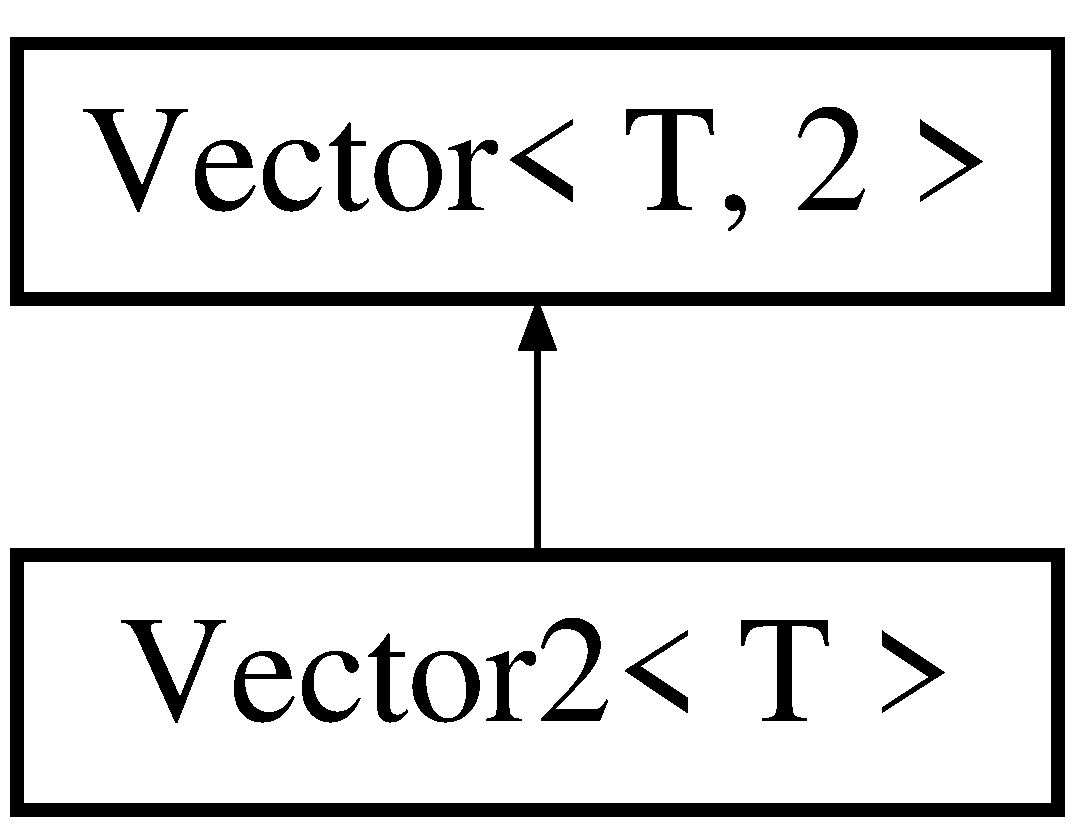
\includegraphics[height=2.000000cm]{class_vector2}
\end{center}
\end{figure}
\subsection*{Public Member Functions}
\begin{DoxyCompactItemize}
\item 
\hyperlink{class_vector2_ae2f1223cb0d664aa73afb789086a4174}{Vector2} ()
\item 
\hyperlink{class_vector2_ac66e49e7814a2c7e394b31d64ed1ba37}{Vector2} (const \hyperlink{class_vector}{Vector}$<$ T, 2 $>$ \&r)
\item 
\hyperlink{class_vector2_ae59e0a10f842521cb7e256ef976ead77}{Vector2} (T x, T y)
\item 
T \hyperlink{class_vector2_a3515bd176ea3f7f5d3558332d4e8467f}{Cross} (const \hyperlink{class_vector2}{Vector2}$<$ T $>$ \&r) const 
\item 
T \hyperlink{class_vector2_ad1dbbb8e7194e7714f8fa85b49e783c7}{Get\+X} () const 
\item 
T \hyperlink{class_vector2_a6be400ba8f30a9cb44f34826e22d28c8}{Get\+Y} () const 
\item 
void \hyperlink{class_vector2_a40af8778aa3d4094a7849389984460a8}{Set\+X} (const T \&x)
\item 
void \hyperlink{class_vector2_abf18c31b0d573b7bf92b8fd91273a08a}{Set\+Y} (const T \&y)
\item 
void \hyperlink{class_vector2_a65267bb2252d019925fdb559b85bdc41}{Set} (const T \&x, const T \&y)
\item 
bt\+Vector3 \hyperlink{class_vector2_a580ec50e199edca4b6ba2db0782367f1}{Get\+B\+T} () const 
\end{DoxyCompactItemize}
\subsection*{Static Public Member Functions}
\begin{DoxyCompactItemize}
\item 
static \hyperlink{class_vector2}{Vector2}$<$ T $>$ \hyperlink{class_vector2_a748ff48f8dae7878c48c0dc71512321d}{Get\+F\+T} (const bt\+Vector3 \&bt)
\end{DoxyCompactItemize}


\subsection{Constructor \& Destructor Documentation}
\hypertarget{class_vector2_ae2f1223cb0d664aa73afb789086a4174}{}\index{Vector2@{Vector2}!Vector2@{Vector2}}
\index{Vector2@{Vector2}!Vector2@{Vector2}}
\subsubsection[{Vector2()}]{\setlength{\rightskip}{0pt plus 5cm}template$<$typename T$>$ {\bf Vector2}$<$ T $>$\+::{\bf Vector2} (
\begin{DoxyParamCaption}
{}
\end{DoxyParamCaption}
)\hspace{0.3cm}{\ttfamily [inline]}}\label{class_vector2_ae2f1223cb0d664aa73afb789086a4174}
\hypertarget{class_vector2_ac66e49e7814a2c7e394b31d64ed1ba37}{}\index{Vector2@{Vector2}!Vector2@{Vector2}}
\index{Vector2@{Vector2}!Vector2@{Vector2}}
\subsubsection[{Vector2(const Vector$<$ T, 2 $>$ \&r)}]{\setlength{\rightskip}{0pt plus 5cm}template$<$typename T$>$ {\bf Vector2}$<$ T $>$\+::{\bf Vector2} (
\begin{DoxyParamCaption}
\item[{const {\bf Vector}$<$ T, 2 $>$ \&}]{r}
\end{DoxyParamCaption}
)\hspace{0.3cm}{\ttfamily [inline]}}\label{class_vector2_ac66e49e7814a2c7e394b31d64ed1ba37}
\hypertarget{class_vector2_ae59e0a10f842521cb7e256ef976ead77}{}\index{Vector2@{Vector2}!Vector2@{Vector2}}
\index{Vector2@{Vector2}!Vector2@{Vector2}}
\subsubsection[{Vector2(\+T x, T y)}]{\setlength{\rightskip}{0pt plus 5cm}template$<$typename T$>$ {\bf Vector2}$<$ T $>$\+::{\bf Vector2} (
\begin{DoxyParamCaption}
\item[{T}]{x, }
\item[{T}]{y}
\end{DoxyParamCaption}
)\hspace{0.3cm}{\ttfamily [inline]}}\label{class_vector2_ae59e0a10f842521cb7e256ef976ead77}


\subsection{Member Function Documentation}
\hypertarget{class_vector2_a3515bd176ea3f7f5d3558332d4e8467f}{}\index{Vector2@{Vector2}!Cross@{Cross}}
\index{Cross@{Cross}!Vector2@{Vector2}}
\subsubsection[{Cross(const Vector2$<$ T $>$ \&r) const }]{\setlength{\rightskip}{0pt plus 5cm}template$<$typename T$>$ T {\bf Vector2}$<$ T $>$\+::Cross (
\begin{DoxyParamCaption}
\item[{const {\bf Vector2}$<$ T $>$ \&}]{r}
\end{DoxyParamCaption}
) const\hspace{0.3cm}{\ttfamily [inline]}}\label{class_vector2_a3515bd176ea3f7f5d3558332d4e8467f}
\hypertarget{class_vector2_a580ec50e199edca4b6ba2db0782367f1}{}\index{Vector2@{Vector2}!Get\+B\+T@{Get\+B\+T}}
\index{Get\+B\+T@{Get\+B\+T}!Vector2@{Vector2}}
\subsubsection[{Get\+B\+T() const }]{\setlength{\rightskip}{0pt plus 5cm}template$<$typename T$>$ bt\+Vector3 {\bf Vector2}$<$ T $>$\+::Get\+B\+T (
\begin{DoxyParamCaption}
{}
\end{DoxyParamCaption}
) const\hspace{0.3cm}{\ttfamily [inline]}}\label{class_vector2_a580ec50e199edca4b6ba2db0782367f1}
\hypertarget{class_vector2_a748ff48f8dae7878c48c0dc71512321d}{}\index{Vector2@{Vector2}!Get\+F\+T@{Get\+F\+T}}
\index{Get\+F\+T@{Get\+F\+T}!Vector2@{Vector2}}
\subsubsection[{Get\+F\+T(const bt\+Vector3 \&bt)}]{\setlength{\rightskip}{0pt plus 5cm}template$<$typename T$>$ static {\bf Vector2}$<$T$>$ {\bf Vector2}$<$ T $>$\+::Get\+F\+T (
\begin{DoxyParamCaption}
\item[{const bt\+Vector3 \&}]{bt}
\end{DoxyParamCaption}
)\hspace{0.3cm}{\ttfamily [inline]}, {\ttfamily [static]}}\label{class_vector2_a748ff48f8dae7878c48c0dc71512321d}
\hypertarget{class_vector2_ad1dbbb8e7194e7714f8fa85b49e783c7}{}\index{Vector2@{Vector2}!Get\+X@{Get\+X}}
\index{Get\+X@{Get\+X}!Vector2@{Vector2}}
\subsubsection[{Get\+X() const }]{\setlength{\rightskip}{0pt plus 5cm}template$<$typename T$>$ T {\bf Vector2}$<$ T $>$\+::Get\+X (
\begin{DoxyParamCaption}
{}
\end{DoxyParamCaption}
) const\hspace{0.3cm}{\ttfamily [inline]}}\label{class_vector2_ad1dbbb8e7194e7714f8fa85b49e783c7}
\hypertarget{class_vector2_a6be400ba8f30a9cb44f34826e22d28c8}{}\index{Vector2@{Vector2}!Get\+Y@{Get\+Y}}
\index{Get\+Y@{Get\+Y}!Vector2@{Vector2}}
\subsubsection[{Get\+Y() const }]{\setlength{\rightskip}{0pt plus 5cm}template$<$typename T$>$ T {\bf Vector2}$<$ T $>$\+::Get\+Y (
\begin{DoxyParamCaption}
{}
\end{DoxyParamCaption}
) const\hspace{0.3cm}{\ttfamily [inline]}}\label{class_vector2_a6be400ba8f30a9cb44f34826e22d28c8}
\hypertarget{class_vector2_a65267bb2252d019925fdb559b85bdc41}{}\index{Vector2@{Vector2}!Set@{Set}}
\index{Set@{Set}!Vector2@{Vector2}}
\subsubsection[{Set(const T \&x, const T \&y)}]{\setlength{\rightskip}{0pt plus 5cm}template$<$typename T$>$ void {\bf Vector2}$<$ T $>$\+::Set (
\begin{DoxyParamCaption}
\item[{const T \&}]{x, }
\item[{const T \&}]{y}
\end{DoxyParamCaption}
)\hspace{0.3cm}{\ttfamily [inline]}}\label{class_vector2_a65267bb2252d019925fdb559b85bdc41}
\hypertarget{class_vector2_a40af8778aa3d4094a7849389984460a8}{}\index{Vector2@{Vector2}!Set\+X@{Set\+X}}
\index{Set\+X@{Set\+X}!Vector2@{Vector2}}
\subsubsection[{Set\+X(const T \&x)}]{\setlength{\rightskip}{0pt plus 5cm}template$<$typename T$>$ void {\bf Vector2}$<$ T $>$\+::Set\+X (
\begin{DoxyParamCaption}
\item[{const T \&}]{x}
\end{DoxyParamCaption}
)\hspace{0.3cm}{\ttfamily [inline]}}\label{class_vector2_a40af8778aa3d4094a7849389984460a8}
\hypertarget{class_vector2_abf18c31b0d573b7bf92b8fd91273a08a}{}\index{Vector2@{Vector2}!Set\+Y@{Set\+Y}}
\index{Set\+Y@{Set\+Y}!Vector2@{Vector2}}
\subsubsection[{Set\+Y(const T \&y)}]{\setlength{\rightskip}{0pt plus 5cm}template$<$typename T$>$ void {\bf Vector2}$<$ T $>$\+::Set\+Y (
\begin{DoxyParamCaption}
\item[{const T \&}]{y}
\end{DoxyParamCaption}
)\hspace{0.3cm}{\ttfamily [inline]}}\label{class_vector2_abf18c31b0d573b7bf92b8fd91273a08a}


The documentation for this class was generated from the following file\+:\begin{DoxyCompactItemize}
\item 
F\+:/\+Fusion3\+D\+\_\+work/src/core/\hyperlink{math3d_8h}{math3d.\+h}\end{DoxyCompactItemize}

\hypertarget{class_vector3}{}\section{Vector3$<$ T $>$ Class Template Reference}
\label{class_vector3}\index{Vector3$<$ T $>$@{Vector3$<$ T $>$}}


{\ttfamily \#include $<$math3d.\+h$>$}

Inheritance diagram for Vector3$<$ T $>$\+:\begin{figure}[H]
\begin{center}
\leavevmode
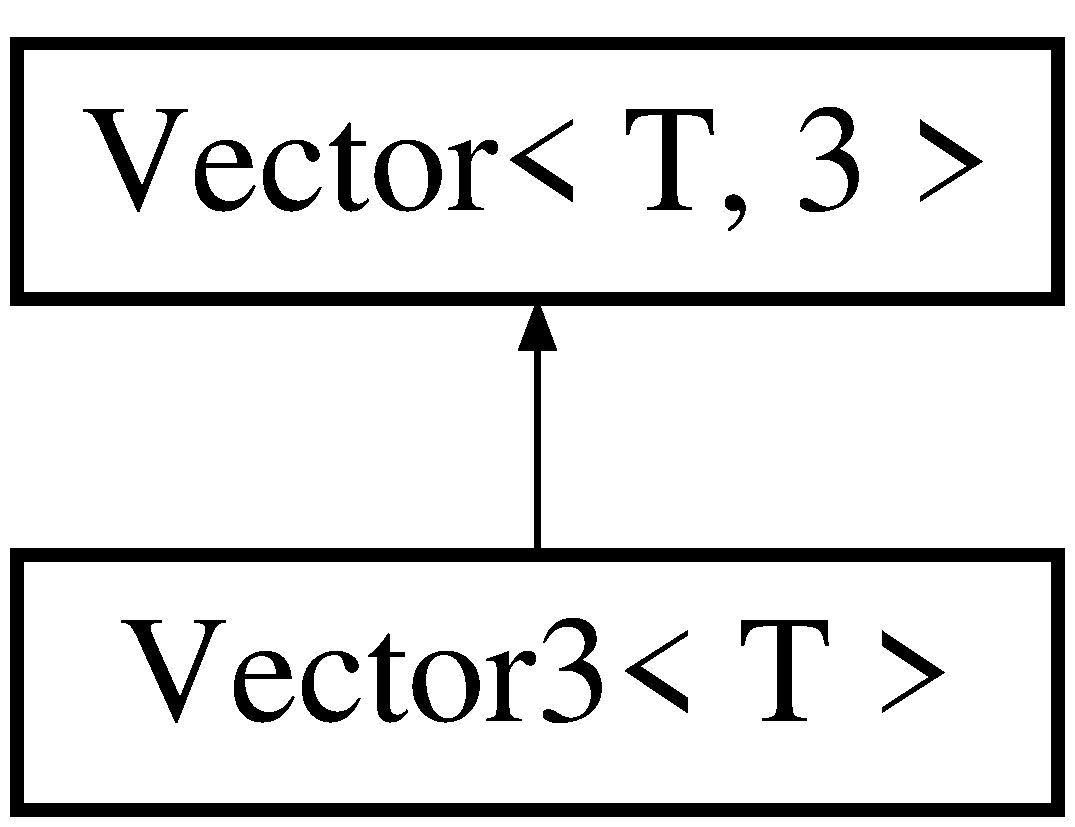
\includegraphics[height=2.000000cm]{class_vector3}
\end{center}
\end{figure}
\subsection*{Public Member Functions}
\begin{DoxyCompactItemize}
\item 
\hyperlink{class_vector3_a54f99f4211298d5245ea578bdd5143cc}{Vector3} ()
\item 
\hyperlink{class_vector3_a7e08c09700f976416b4692a077087615}{Vector3} (const \hyperlink{class_vector}{Vector}$<$ T, 3 $>$ \&r)
\item 
\hyperlink{class_vector3_a6797fe2b04a56b6b2ee517f23876ebab}{Vector3} (T x, T y, T z)
\item 
\hyperlink{class_vector3}{Vector3}$<$ T $>$ \hyperlink{class_vector3_a5ad3b7c9135180b76c48e47c95e6f93d}{Cross} (const \hyperlink{class_vector3}{Vector3}$<$ T $>$ \&r) const 
\item 
\hyperlink{class_vector3}{Vector3}$<$ T $>$ \hyperlink{class_vector3_a6d9ae17426f8721e5918003d9af027a7}{Rotate} (T angle, const \hyperlink{class_vector3}{Vector3}$<$ T $>$ \&axis) const 
\item 
\hyperlink{class_vector2}{Vector2}$<$ T $>$ \hyperlink{class_vector3_a8a5ca6e62a38b02ccdbdc17542873e61}{Get\+X\+Y} () const 
\item 
\hyperlink{class_vector2}{Vector2}$<$ T $>$ \hyperlink{class_vector3_af022b910b5a1d276745fd7be0b70daa7}{Get\+Y\+Z} () const 
\item 
\hyperlink{class_vector2}{Vector2}$<$ T $>$ \hyperlink{class_vector3_ae84d69bb63b947a449a7f9f6b022c1c4}{Get\+Z\+X} () const 
\item 
\hyperlink{class_vector2}{Vector2}$<$ T $>$ \hyperlink{class_vector3_a1d9b1de4017804cf39b2fca3ce3a1e41}{Get\+Y\+X} () const 
\item 
\hyperlink{class_vector2}{Vector2}$<$ T $>$ \hyperlink{class_vector3_af2ceba0c92219a584a599f9c7c493de6}{Get\+Z\+Y} () const 
\item 
\hyperlink{class_vector2}{Vector2}$<$ T $>$ \hyperlink{class_vector3_ad0004bbe1d6cf77e9e0e419102a093ad}{Get\+X\+Z} () const 
\item 
T \hyperlink{class_vector3_a7ebe403dc3badb8e5943a043a01d1dc6}{Get\+X} () const 
\item 
T \hyperlink{class_vector3_a2cb5b82371d17c70d8d37002d3300e76}{Get\+Y} () const 
\item 
T \hyperlink{class_vector3_ad6da696280e32d7b14ef897977e27f5a}{Get\+Z} () const 
\item 
void \hyperlink{class_vector3_ab447da00bb0176f3160edb743a7a0a19}{Set\+X} (const T \&x)
\item 
void \hyperlink{class_vector3_a65b71b95a49861281fcc60be10354d89}{Set\+Y} (const T \&y)
\item 
void \hyperlink{class_vector3_adc178cec4d4770d59881f19c5335edfe}{Set\+Z} (const T \&z)
\item 
void \hyperlink{class_vector3_af1f7474d44998863ad66e5e3c8221f9b}{Set} (const T \&x, const T \&y, const T \&z)
\item 
bt\+Vector3 \hyperlink{class_vector3_a95fadde3d5f34be5d64d1fee74d657fc}{Get\+B\+T} () const 
\end{DoxyCompactItemize}
\subsection*{Static Public Member Functions}
\begin{DoxyCompactItemize}
\item 
static \hyperlink{class_vector3}{Vector3}$<$ T $>$ \hyperlink{class_vector3_ad410b40f5f96cf2cd27f779767111fb3}{Get\+F\+T} (const bt\+Vector3 \&bt)
\end{DoxyCompactItemize}


\subsection{Constructor \& Destructor Documentation}
\hypertarget{class_vector3_a54f99f4211298d5245ea578bdd5143cc}{}\index{Vector3@{Vector3}!Vector3@{Vector3}}
\index{Vector3@{Vector3}!Vector3@{Vector3}}
\subsubsection[{Vector3()}]{\setlength{\rightskip}{0pt plus 5cm}template$<$typename T$>$ {\bf Vector3}$<$ T $>$\+::{\bf Vector3} (
\begin{DoxyParamCaption}
{}
\end{DoxyParamCaption}
)\hspace{0.3cm}{\ttfamily [inline]}}\label{class_vector3_a54f99f4211298d5245ea578bdd5143cc}
\hypertarget{class_vector3_a7e08c09700f976416b4692a077087615}{}\index{Vector3@{Vector3}!Vector3@{Vector3}}
\index{Vector3@{Vector3}!Vector3@{Vector3}}
\subsubsection[{Vector3(const Vector$<$ T, 3 $>$ \&r)}]{\setlength{\rightskip}{0pt plus 5cm}template$<$typename T$>$ {\bf Vector3}$<$ T $>$\+::{\bf Vector3} (
\begin{DoxyParamCaption}
\item[{const {\bf Vector}$<$ T, 3 $>$ \&}]{r}
\end{DoxyParamCaption}
)\hspace{0.3cm}{\ttfamily [inline]}}\label{class_vector3_a7e08c09700f976416b4692a077087615}
\hypertarget{class_vector3_a6797fe2b04a56b6b2ee517f23876ebab}{}\index{Vector3@{Vector3}!Vector3@{Vector3}}
\index{Vector3@{Vector3}!Vector3@{Vector3}}
\subsubsection[{Vector3(\+T x, T y, T z)}]{\setlength{\rightskip}{0pt plus 5cm}template$<$typename T$>$ {\bf Vector3}$<$ T $>$\+::{\bf Vector3} (
\begin{DoxyParamCaption}
\item[{T}]{x, }
\item[{T}]{y, }
\item[{T}]{z}
\end{DoxyParamCaption}
)\hspace{0.3cm}{\ttfamily [inline]}}\label{class_vector3_a6797fe2b04a56b6b2ee517f23876ebab}


\subsection{Member Function Documentation}
\hypertarget{class_vector3_a5ad3b7c9135180b76c48e47c95e6f93d}{}\index{Vector3@{Vector3}!Cross@{Cross}}
\index{Cross@{Cross}!Vector3@{Vector3}}
\subsubsection[{Cross(const Vector3$<$ T $>$ \&r) const }]{\setlength{\rightskip}{0pt plus 5cm}template$<$typename T$>$ {\bf Vector3}$<$T$>$ {\bf Vector3}$<$ T $>$\+::Cross (
\begin{DoxyParamCaption}
\item[{const {\bf Vector3}$<$ T $>$ \&}]{r}
\end{DoxyParamCaption}
) const\hspace{0.3cm}{\ttfamily [inline]}}\label{class_vector3_a5ad3b7c9135180b76c48e47c95e6f93d}
\hypertarget{class_vector3_a95fadde3d5f34be5d64d1fee74d657fc}{}\index{Vector3@{Vector3}!Get\+B\+T@{Get\+B\+T}}
\index{Get\+B\+T@{Get\+B\+T}!Vector3@{Vector3}}
\subsubsection[{Get\+B\+T() const }]{\setlength{\rightskip}{0pt plus 5cm}template$<$typename T$>$ bt\+Vector3 {\bf Vector3}$<$ T $>$\+::Get\+B\+T (
\begin{DoxyParamCaption}
{}
\end{DoxyParamCaption}
) const\hspace{0.3cm}{\ttfamily [inline]}}\label{class_vector3_a95fadde3d5f34be5d64d1fee74d657fc}
\hypertarget{class_vector3_ad410b40f5f96cf2cd27f779767111fb3}{}\index{Vector3@{Vector3}!Get\+F\+T@{Get\+F\+T}}
\index{Get\+F\+T@{Get\+F\+T}!Vector3@{Vector3}}
\subsubsection[{Get\+F\+T(const bt\+Vector3 \&bt)}]{\setlength{\rightskip}{0pt plus 5cm}template$<$typename T$>$ static {\bf Vector3}$<$T$>$ {\bf Vector3}$<$ T $>$\+::Get\+F\+T (
\begin{DoxyParamCaption}
\item[{const bt\+Vector3$<$ T $>$ \&}]{bt}
\end{DoxyParamCaption}
)\hspace{0.3cm}{\ttfamily [inline]}, {\ttfamily [static]}}\label{class_vector3_ad410b40f5f96cf2cd27f779767111fb3}
\hypertarget{class_vector3_a7ebe403dc3badb8e5943a043a01d1dc6}{}\index{Vector3@{Vector3}!Get\+X@{Get\+X}}
\index{Get\+X@{Get\+X}!Vector3@{Vector3}}
\subsubsection[{Get\+X() const }]{\setlength{\rightskip}{0pt plus 5cm}template$<$typename T$>$ T {\bf Vector3}$<$ T $>$\+::Get\+X (
\begin{DoxyParamCaption}
{}
\end{DoxyParamCaption}
) const\hspace{0.3cm}{\ttfamily [inline]}}\label{class_vector3_a7ebe403dc3badb8e5943a043a01d1dc6}
\hypertarget{class_vector3_a8a5ca6e62a38b02ccdbdc17542873e61}{}\index{Vector3@{Vector3}!Get\+X\+Y@{Get\+X\+Y}}
\index{Get\+X\+Y@{Get\+X\+Y}!Vector3@{Vector3}}
\subsubsection[{Get\+X\+Y() const }]{\setlength{\rightskip}{0pt plus 5cm}template$<$typename T$>$ {\bf Vector2}$<$T$>$ {\bf Vector3}$<$ T $>$\+::Get\+X\+Y (
\begin{DoxyParamCaption}
{}
\end{DoxyParamCaption}
) const\hspace{0.3cm}{\ttfamily [inline]}}\label{class_vector3_a8a5ca6e62a38b02ccdbdc17542873e61}
\hypertarget{class_vector3_ad0004bbe1d6cf77e9e0e419102a093ad}{}\index{Vector3@{Vector3}!Get\+X\+Z@{Get\+X\+Z}}
\index{Get\+X\+Z@{Get\+X\+Z}!Vector3@{Vector3}}
\subsubsection[{Get\+X\+Z() const }]{\setlength{\rightskip}{0pt plus 5cm}template$<$typename T$>$ {\bf Vector2}$<$T$>$ {\bf Vector3}$<$ T $>$\+::Get\+X\+Z (
\begin{DoxyParamCaption}
{}
\end{DoxyParamCaption}
) const\hspace{0.3cm}{\ttfamily [inline]}}\label{class_vector3_ad0004bbe1d6cf77e9e0e419102a093ad}
\hypertarget{class_vector3_a2cb5b82371d17c70d8d37002d3300e76}{}\index{Vector3@{Vector3}!Get\+Y@{Get\+Y}}
\index{Get\+Y@{Get\+Y}!Vector3@{Vector3}}
\subsubsection[{Get\+Y() const }]{\setlength{\rightskip}{0pt plus 5cm}template$<$typename T$>$ T {\bf Vector3}$<$ T $>$\+::Get\+Y (
\begin{DoxyParamCaption}
{}
\end{DoxyParamCaption}
) const\hspace{0.3cm}{\ttfamily [inline]}}\label{class_vector3_a2cb5b82371d17c70d8d37002d3300e76}
\hypertarget{class_vector3_a1d9b1de4017804cf39b2fca3ce3a1e41}{}\index{Vector3@{Vector3}!Get\+Y\+X@{Get\+Y\+X}}
\index{Get\+Y\+X@{Get\+Y\+X}!Vector3@{Vector3}}
\subsubsection[{Get\+Y\+X() const }]{\setlength{\rightskip}{0pt plus 5cm}template$<$typename T$>$ {\bf Vector2}$<$T$>$ {\bf Vector3}$<$ T $>$\+::Get\+Y\+X (
\begin{DoxyParamCaption}
{}
\end{DoxyParamCaption}
) const\hspace{0.3cm}{\ttfamily [inline]}}\label{class_vector3_a1d9b1de4017804cf39b2fca3ce3a1e41}
\hypertarget{class_vector3_af022b910b5a1d276745fd7be0b70daa7}{}\index{Vector3@{Vector3}!Get\+Y\+Z@{Get\+Y\+Z}}
\index{Get\+Y\+Z@{Get\+Y\+Z}!Vector3@{Vector3}}
\subsubsection[{Get\+Y\+Z() const }]{\setlength{\rightskip}{0pt plus 5cm}template$<$typename T$>$ {\bf Vector2}$<$T$>$ {\bf Vector3}$<$ T $>$\+::Get\+Y\+Z (
\begin{DoxyParamCaption}
{}
\end{DoxyParamCaption}
) const\hspace{0.3cm}{\ttfamily [inline]}}\label{class_vector3_af022b910b5a1d276745fd7be0b70daa7}
\hypertarget{class_vector3_ad6da696280e32d7b14ef897977e27f5a}{}\index{Vector3@{Vector3}!Get\+Z@{Get\+Z}}
\index{Get\+Z@{Get\+Z}!Vector3@{Vector3}}
\subsubsection[{Get\+Z() const }]{\setlength{\rightskip}{0pt plus 5cm}template$<$typename T$>$ T {\bf Vector3}$<$ T $>$\+::Get\+Z (
\begin{DoxyParamCaption}
{}
\end{DoxyParamCaption}
) const\hspace{0.3cm}{\ttfamily [inline]}}\label{class_vector3_ad6da696280e32d7b14ef897977e27f5a}
\hypertarget{class_vector3_ae84d69bb63b947a449a7f9f6b022c1c4}{}\index{Vector3@{Vector3}!Get\+Z\+X@{Get\+Z\+X}}
\index{Get\+Z\+X@{Get\+Z\+X}!Vector3@{Vector3}}
\subsubsection[{Get\+Z\+X() const }]{\setlength{\rightskip}{0pt plus 5cm}template$<$typename T$>$ {\bf Vector2}$<$T$>$ {\bf Vector3}$<$ T $>$\+::Get\+Z\+X (
\begin{DoxyParamCaption}
{}
\end{DoxyParamCaption}
) const\hspace{0.3cm}{\ttfamily [inline]}}\label{class_vector3_ae84d69bb63b947a449a7f9f6b022c1c4}
\hypertarget{class_vector3_af2ceba0c92219a584a599f9c7c493de6}{}\index{Vector3@{Vector3}!Get\+Z\+Y@{Get\+Z\+Y}}
\index{Get\+Z\+Y@{Get\+Z\+Y}!Vector3@{Vector3}}
\subsubsection[{Get\+Z\+Y() const }]{\setlength{\rightskip}{0pt plus 5cm}template$<$typename T$>$ {\bf Vector2}$<$T$>$ {\bf Vector3}$<$ T $>$\+::Get\+Z\+Y (
\begin{DoxyParamCaption}
{}
\end{DoxyParamCaption}
) const\hspace{0.3cm}{\ttfamily [inline]}}\label{class_vector3_af2ceba0c92219a584a599f9c7c493de6}
\hypertarget{class_vector3_a6d9ae17426f8721e5918003d9af027a7}{}\index{Vector3@{Vector3}!Rotate@{Rotate}}
\index{Rotate@{Rotate}!Vector3@{Vector3}}
\subsubsection[{Rotate(\+T angle, const Vector3$<$ T $>$ \&axis) const }]{\setlength{\rightskip}{0pt plus 5cm}template$<$typename T$>$ {\bf Vector3}$<$T$>$ {\bf Vector3}$<$ T $>$\+::Rotate (
\begin{DoxyParamCaption}
\item[{T}]{angle, }
\item[{const {\bf Vector3}$<$ T $>$ \&}]{axis}
\end{DoxyParamCaption}
) const\hspace{0.3cm}{\ttfamily [inline]}}\label{class_vector3_a6d9ae17426f8721e5918003d9af027a7}
\hypertarget{class_vector3_af1f7474d44998863ad66e5e3c8221f9b}{}\index{Vector3@{Vector3}!Set@{Set}}
\index{Set@{Set}!Vector3@{Vector3}}
\subsubsection[{Set(const T \&x, const T \&y, const T \&z)}]{\setlength{\rightskip}{0pt plus 5cm}template$<$typename T$>$ void {\bf Vector3}$<$ T $>$\+::Set (
\begin{DoxyParamCaption}
\item[{const T \&}]{x, }
\item[{const T \&}]{y, }
\item[{const T \&}]{z}
\end{DoxyParamCaption}
)\hspace{0.3cm}{\ttfamily [inline]}}\label{class_vector3_af1f7474d44998863ad66e5e3c8221f9b}
\hypertarget{class_vector3_ab447da00bb0176f3160edb743a7a0a19}{}\index{Vector3@{Vector3}!Set\+X@{Set\+X}}
\index{Set\+X@{Set\+X}!Vector3@{Vector3}}
\subsubsection[{Set\+X(const T \&x)}]{\setlength{\rightskip}{0pt plus 5cm}template$<$typename T$>$ void {\bf Vector3}$<$ T $>$\+::Set\+X (
\begin{DoxyParamCaption}
\item[{const T \&}]{x}
\end{DoxyParamCaption}
)\hspace{0.3cm}{\ttfamily [inline]}}\label{class_vector3_ab447da00bb0176f3160edb743a7a0a19}
\hypertarget{class_vector3_a65b71b95a49861281fcc60be10354d89}{}\index{Vector3@{Vector3}!Set\+Y@{Set\+Y}}
\index{Set\+Y@{Set\+Y}!Vector3@{Vector3}}
\subsubsection[{Set\+Y(const T \&y)}]{\setlength{\rightskip}{0pt plus 5cm}template$<$typename T$>$ void {\bf Vector3}$<$ T $>$\+::Set\+Y (
\begin{DoxyParamCaption}
\item[{const T \&}]{y}
\end{DoxyParamCaption}
)\hspace{0.3cm}{\ttfamily [inline]}}\label{class_vector3_a65b71b95a49861281fcc60be10354d89}
\hypertarget{class_vector3_adc178cec4d4770d59881f19c5335edfe}{}\index{Vector3@{Vector3}!Set\+Z@{Set\+Z}}
\index{Set\+Z@{Set\+Z}!Vector3@{Vector3}}
\subsubsection[{Set\+Z(const T \&z)}]{\setlength{\rightskip}{0pt plus 5cm}template$<$typename T$>$ void {\bf Vector3}$<$ T $>$\+::Set\+Z (
\begin{DoxyParamCaption}
\item[{const T \&}]{z}
\end{DoxyParamCaption}
)\hspace{0.3cm}{\ttfamily [inline]}}\label{class_vector3_adc178cec4d4770d59881f19c5335edfe}


The documentation for this class was generated from the following file\+:\begin{DoxyCompactItemize}
\item 
F\+:/\+Fusion3\+D\+\_\+work/src/core/\hyperlink{math3d_8h}{math3d.\+h}\end{DoxyCompactItemize}

\hypertarget{class_vector3f}{}\section{Vector3f Class Reference}
\label{class_vector3f}\index{Vector3f@{Vector3f}}


{\ttfamily \#include $<$math3d.\+h$>$}

Inheritance diagram for Vector3f\+:\begin{figure}[H]
\begin{center}
\leavevmode
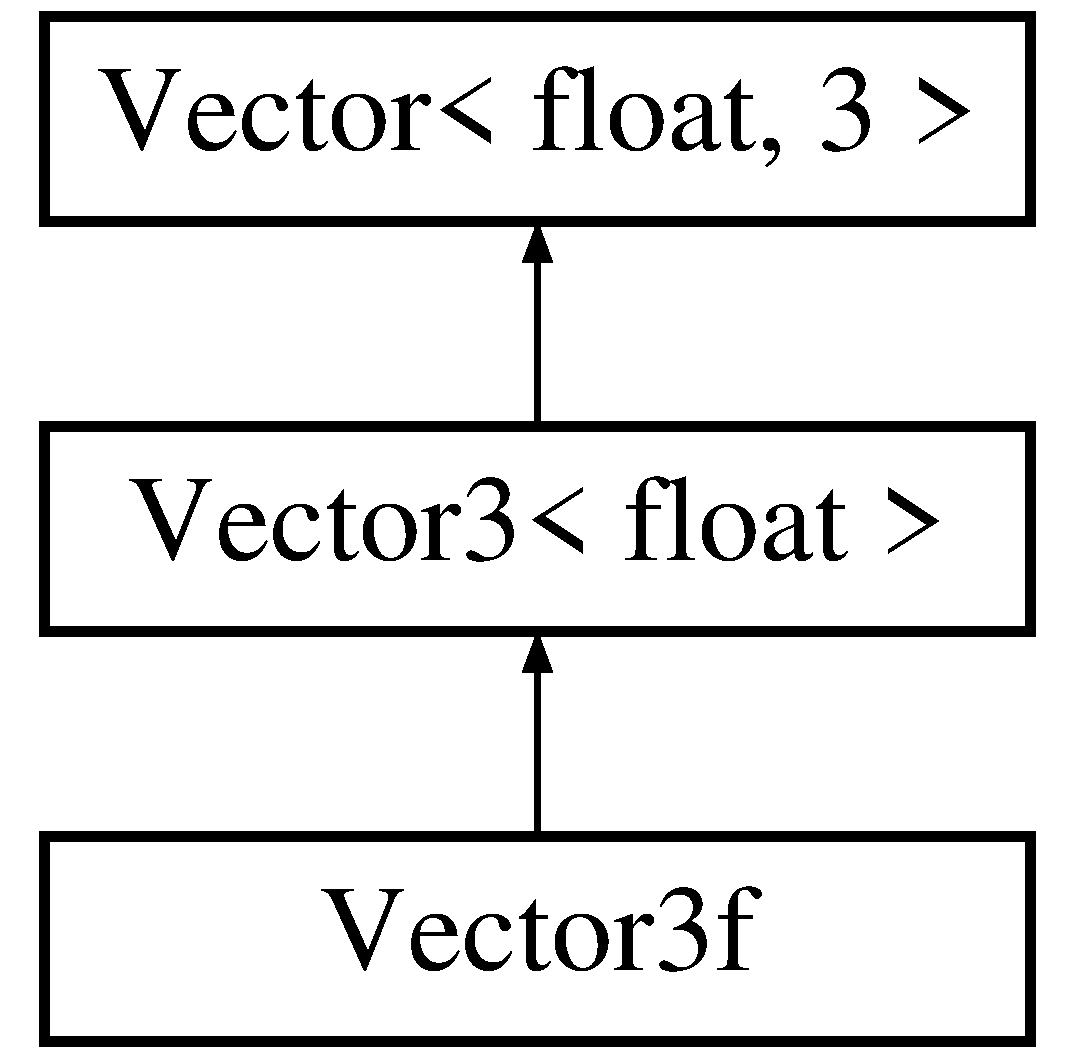
\includegraphics[height=3.000000cm]{class_vector3f}
\end{center}
\end{figure}
\subsection*{Public Member Functions}
\begin{DoxyCompactItemize}
\item 
\hyperlink{class_vector3f_a83ea28e272c27ddaa8c0d2c703850bcb}{Vector3f} (float x=0.\+0f, float y=0.\+0f, float z=0.\+0f)
\item 
\hyperlink{class_vector3f_adf12e9520dbe1870db90f61da7c7e439}{Vector3f} (const \hyperlink{class_vector3}{Vector3}$<$ float $>$ \&r)
\item 
float \hyperlink{class_vector3f_a355e21a71ae0d55ae26ccf2a3739a4e1}{Length} () const 
\item 
float \hyperlink{class_vector3f_a971a55e8f4724edcad60f5b14f953906}{Dot} (const \hyperlink{class_vector3f}{Vector3f} \&v) const 
\item 
\hyperlink{class_vector3f}{Vector3f} \hyperlink{class_vector3f_aa08a1a02eb2e991f26231edeb0811acf}{Cross} (const \hyperlink{class_vector3f}{Vector3f} \&v) const 
\item 
\hyperlink{class_vector3f}{Vector3f} \hyperlink{class_vector3f_a64cb066d442f06446d34790fbee18423}{Rotate} (float angle, const \hyperlink{class_vector3f}{Vector3f} \&axis) const 
\item 
\hyperlink{class_vector3f}{Vector3f} \hyperlink{class_vector3f_a352f95e22f448bb5ba17d44077db0a92}{Rotate} (const \hyperlink{class_quaternion}{Quaternion} \&rotation) const 
\item 
\hyperlink{class_vector3f}{Vector3f} \hyperlink{class_vector3f_a96d4153d8f724afc0da1ad0d9a78b358}{Normalized} () const 
\item 
\hyperlink{class_vector3f}{Vector3f} \hyperlink{class_vector3f_af045d6419eba34fecf0a06d5f05950ec}{operator+} (const \hyperlink{class_vector3f}{Vector3f} \&r) const 
\item 
\hyperlink{class_vector3f}{Vector3f} \hyperlink{class_vector3f_a2fdf46c83defdd5de1286aeda25cdbcb}{operator-\/} (const \hyperlink{class_vector3f}{Vector3f} \&r) const 
\item 
\hyperlink{class_vector3f}{Vector3f} \hyperlink{class_vector3f_a7e7fe965ab6b026df5494fff5d8f5080}{operator$\ast$} (float f) const 
\item 
\hyperlink{class_vector3f}{Vector3f} \hyperlink{class_vector3f_aa57991e73045b5f57216e1020bda021a}{operator/} (float f) const 
\item 
bool \hyperlink{class_vector3f_acfee43096f6cdfa042fab3defe7c253b}{operator==} (const \hyperlink{class_vector3f}{Vector3f} \&r) const 
\item 
bool \hyperlink{class_vector3f_ab41ff6fe5ca06f605499dfa7668c3eb8}{operator!=} (const \hyperlink{class_vector3f}{Vector3f} \&r) const 
\item 
\hyperlink{class_vector3f}{Vector3f} \& \hyperlink{class_vector3f_abb9089cd5b410ea28b1d1db63fc550f8}{operator+=} (const \hyperlink{class_vector3f}{Vector3f} \&r)
\item 
\hyperlink{class_vector3f}{Vector3f} \& \hyperlink{class_vector3f_a63ec561fd67ea011aa973c0549d48a26}{operator-\/=} (const \hyperlink{class_vector3f}{Vector3f} \&r)
\item 
\hyperlink{class_vector3f}{Vector3f} \& \hyperlink{class_vector3f_a0449c07194a079d3eb57961e374e96ee}{operator$\ast$=} (float f)
\item 
\hyperlink{class_vector3f}{Vector3f} \& \hyperlink{class_vector3f_a7586bd129a4aa5326d4663323760958f}{operator/=} (float f)
\item 
float \hyperlink{class_vector3f_af5a97e51e8e1db09c7381a9d15e8f176}{Get\+X} () const 
\item 
float \hyperlink{class_vector3f_a468098deabbe5e8bef23e555a974b3af}{Get\+Y} () const 
\item 
float \hyperlink{class_vector3f_a5e6d015d4cf9fa85eeb51e0e53225d84}{Get\+Z} () const 
\item 
void \hyperlink{class_vector3f_aaa6791fa256647707bcf41017f498bcf}{Set\+X} (float x)
\item 
void \hyperlink{class_vector3f_a260bcd7eb6bebb43f79a29421d254f2b}{Set\+Y} (float y)
\item 
void \hyperlink{class_vector3f_afb24d616af2e75cce9af632c870141ac}{Set\+Z} (float z)
\item 
void \hyperlink{class_vector3f_abbbcad97c6edc42ad313482fbb4eb3dd}{Set} (float x, float y, float z)
\end{DoxyCompactItemize}
\subsection*{Additional Inherited Members}


\subsection{Constructor \& Destructor Documentation}
\hypertarget{class_vector3f_a83ea28e272c27ddaa8c0d2c703850bcb}{}\index{Vector3f@{Vector3f}!Vector3f@{Vector3f}}
\index{Vector3f@{Vector3f}!Vector3f@{Vector3f}}
\subsubsection[{Vector3f(float x=0.\+0f, float y=0.\+0f, float z=0.\+0f)}]{\setlength{\rightskip}{0pt plus 5cm}Vector3f\+::\+Vector3f (
\begin{DoxyParamCaption}
\item[{float}]{x = {\ttfamily 0.0f}, }
\item[{float}]{y = {\ttfamily 0.0f}, }
\item[{float}]{z = {\ttfamily 0.0f}}
\end{DoxyParamCaption}
)\hspace{0.3cm}{\ttfamily [inline]}}\label{class_vector3f_a83ea28e272c27ddaa8c0d2c703850bcb}
\hypertarget{class_vector3f_adf12e9520dbe1870db90f61da7c7e439}{}\index{Vector3f@{Vector3f}!Vector3f@{Vector3f}}
\index{Vector3f@{Vector3f}!Vector3f@{Vector3f}}
\subsubsection[{Vector3f(const Vector3$<$ float $>$ \&r)}]{\setlength{\rightskip}{0pt plus 5cm}Vector3f\+::\+Vector3f (
\begin{DoxyParamCaption}
\item[{const {\bf Vector3}$<$ float $>$ \&}]{r}
\end{DoxyParamCaption}
)\hspace{0.3cm}{\ttfamily [inline]}}\label{class_vector3f_adf12e9520dbe1870db90f61da7c7e439}


\subsection{Member Function Documentation}
\hypertarget{class_vector3f_aa08a1a02eb2e991f26231edeb0811acf}{}\index{Vector3f@{Vector3f}!Cross@{Cross}}
\index{Cross@{Cross}!Vector3f@{Vector3f}}
\subsubsection[{Cross(const Vector3f \&v) const }]{\setlength{\rightskip}{0pt plus 5cm}{\bf Vector3f} Vector3f\+::\+Cross (
\begin{DoxyParamCaption}
\item[{const {\bf Vector3f} \&}]{v}
\end{DoxyParamCaption}
) const\hspace{0.3cm}{\ttfamily [inline]}}\label{class_vector3f_aa08a1a02eb2e991f26231edeb0811acf}
\hypertarget{class_vector3f_a971a55e8f4724edcad60f5b14f953906}{}\index{Vector3f@{Vector3f}!Dot@{Dot}}
\index{Dot@{Dot}!Vector3f@{Vector3f}}
\subsubsection[{Dot(const Vector3f \&v) const }]{\setlength{\rightskip}{0pt plus 5cm}float Vector3f\+::\+Dot (
\begin{DoxyParamCaption}
\item[{const {\bf Vector3f} \&}]{v}
\end{DoxyParamCaption}
) const\hspace{0.3cm}{\ttfamily [inline]}}\label{class_vector3f_a971a55e8f4724edcad60f5b14f953906}
\hypertarget{class_vector3f_af5a97e51e8e1db09c7381a9d15e8f176}{}\index{Vector3f@{Vector3f}!Get\+X@{Get\+X}}
\index{Get\+X@{Get\+X}!Vector3f@{Vector3f}}
\subsubsection[{Get\+X() const }]{\setlength{\rightskip}{0pt plus 5cm}float Vector3f\+::\+Get\+X (
\begin{DoxyParamCaption}
{}
\end{DoxyParamCaption}
) const\hspace{0.3cm}{\ttfamily [inline]}}\label{class_vector3f_af5a97e51e8e1db09c7381a9d15e8f176}
\hypertarget{class_vector3f_a468098deabbe5e8bef23e555a974b3af}{}\index{Vector3f@{Vector3f}!Get\+Y@{Get\+Y}}
\index{Get\+Y@{Get\+Y}!Vector3f@{Vector3f}}
\subsubsection[{Get\+Y() const }]{\setlength{\rightskip}{0pt plus 5cm}float Vector3f\+::\+Get\+Y (
\begin{DoxyParamCaption}
{}
\end{DoxyParamCaption}
) const\hspace{0.3cm}{\ttfamily [inline]}}\label{class_vector3f_a468098deabbe5e8bef23e555a974b3af}
\hypertarget{class_vector3f_a5e6d015d4cf9fa85eeb51e0e53225d84}{}\index{Vector3f@{Vector3f}!Get\+Z@{Get\+Z}}
\index{Get\+Z@{Get\+Z}!Vector3f@{Vector3f}}
\subsubsection[{Get\+Z() const }]{\setlength{\rightskip}{0pt plus 5cm}float Vector3f\+::\+Get\+Z (
\begin{DoxyParamCaption}
{}
\end{DoxyParamCaption}
) const\hspace{0.3cm}{\ttfamily [inline]}}\label{class_vector3f_a5e6d015d4cf9fa85eeb51e0e53225d84}
\hypertarget{class_vector3f_a355e21a71ae0d55ae26ccf2a3739a4e1}{}\index{Vector3f@{Vector3f}!Length@{Length}}
\index{Length@{Length}!Vector3f@{Vector3f}}
\subsubsection[{Length() const }]{\setlength{\rightskip}{0pt plus 5cm}float Vector3f\+::\+Length (
\begin{DoxyParamCaption}
{}
\end{DoxyParamCaption}
) const\hspace{0.3cm}{\ttfamily [inline]}}\label{class_vector3f_a355e21a71ae0d55ae26ccf2a3739a4e1}
\hypertarget{class_vector3f_a96d4153d8f724afc0da1ad0d9a78b358}{}\index{Vector3f@{Vector3f}!Normalized@{Normalized}}
\index{Normalized@{Normalized}!Vector3f@{Vector3f}}
\subsubsection[{Normalized() const }]{\setlength{\rightskip}{0pt plus 5cm}{\bf Vector3f} Vector3f\+::\+Normalized (
\begin{DoxyParamCaption}
{}
\end{DoxyParamCaption}
) const\hspace{0.3cm}{\ttfamily [inline]}}\label{class_vector3f_a96d4153d8f724afc0da1ad0d9a78b358}
\hypertarget{class_vector3f_ab41ff6fe5ca06f605499dfa7668c3eb8}{}\index{Vector3f@{Vector3f}!operator"!=@{operator"!=}}
\index{operator"!=@{operator"!=}!Vector3f@{Vector3f}}
\subsubsection[{operator"!=(const Vector3f \&r) const }]{\setlength{\rightskip}{0pt plus 5cm}bool Vector3f\+::operator!= (
\begin{DoxyParamCaption}
\item[{const {\bf Vector3f} \&}]{r}
\end{DoxyParamCaption}
) const\hspace{0.3cm}{\ttfamily [inline]}}\label{class_vector3f_ab41ff6fe5ca06f605499dfa7668c3eb8}
\hypertarget{class_vector3f_a7e7fe965ab6b026df5494fff5d8f5080}{}\index{Vector3f@{Vector3f}!operator$\ast$@{operator$\ast$}}
\index{operator$\ast$@{operator$\ast$}!Vector3f@{Vector3f}}
\subsubsection[{operator$\ast$(float f) const }]{\setlength{\rightskip}{0pt plus 5cm}{\bf Vector3f} Vector3f\+::operator$\ast$ (
\begin{DoxyParamCaption}
\item[{float}]{f}
\end{DoxyParamCaption}
) const\hspace{0.3cm}{\ttfamily [inline]}}\label{class_vector3f_a7e7fe965ab6b026df5494fff5d8f5080}
\hypertarget{class_vector3f_a0449c07194a079d3eb57961e374e96ee}{}\index{Vector3f@{Vector3f}!operator$\ast$=@{operator$\ast$=}}
\index{operator$\ast$=@{operator$\ast$=}!Vector3f@{Vector3f}}
\subsubsection[{operator$\ast$=(float f)}]{\setlength{\rightskip}{0pt plus 5cm}{\bf Vector3f}\& Vector3f\+::operator$\ast$= (
\begin{DoxyParamCaption}
\item[{float}]{f}
\end{DoxyParamCaption}
)\hspace{0.3cm}{\ttfamily [inline]}}\label{class_vector3f_a0449c07194a079d3eb57961e374e96ee}
\hypertarget{class_vector3f_af045d6419eba34fecf0a06d5f05950ec}{}\index{Vector3f@{Vector3f}!operator+@{operator+}}
\index{operator+@{operator+}!Vector3f@{Vector3f}}
\subsubsection[{operator+(const Vector3f \&r) const }]{\setlength{\rightskip}{0pt plus 5cm}{\bf Vector3f} Vector3f\+::operator+ (
\begin{DoxyParamCaption}
\item[{const {\bf Vector3f} \&}]{r}
\end{DoxyParamCaption}
) const\hspace{0.3cm}{\ttfamily [inline]}}\label{class_vector3f_af045d6419eba34fecf0a06d5f05950ec}
\hypertarget{class_vector3f_abb9089cd5b410ea28b1d1db63fc550f8}{}\index{Vector3f@{Vector3f}!operator+=@{operator+=}}
\index{operator+=@{operator+=}!Vector3f@{Vector3f}}
\subsubsection[{operator+=(const Vector3f \&r)}]{\setlength{\rightskip}{0pt plus 5cm}{\bf Vector3f}\& Vector3f\+::operator+= (
\begin{DoxyParamCaption}
\item[{const {\bf Vector3f} \&}]{r}
\end{DoxyParamCaption}
)\hspace{0.3cm}{\ttfamily [inline]}}\label{class_vector3f_abb9089cd5b410ea28b1d1db63fc550f8}
\hypertarget{class_vector3f_a2fdf46c83defdd5de1286aeda25cdbcb}{}\index{Vector3f@{Vector3f}!operator-\/@{operator-\/}}
\index{operator-\/@{operator-\/}!Vector3f@{Vector3f}}
\subsubsection[{operator-\/(const Vector3f \&r) const }]{\setlength{\rightskip}{0pt plus 5cm}{\bf Vector3f} Vector3f\+::operator-\/ (
\begin{DoxyParamCaption}
\item[{const {\bf Vector3f} \&}]{r}
\end{DoxyParamCaption}
) const\hspace{0.3cm}{\ttfamily [inline]}}\label{class_vector3f_a2fdf46c83defdd5de1286aeda25cdbcb}
\hypertarget{class_vector3f_a63ec561fd67ea011aa973c0549d48a26}{}\index{Vector3f@{Vector3f}!operator-\/=@{operator-\/=}}
\index{operator-\/=@{operator-\/=}!Vector3f@{Vector3f}}
\subsubsection[{operator-\/=(const Vector3f \&r)}]{\setlength{\rightskip}{0pt plus 5cm}{\bf Vector3f}\& Vector3f\+::operator-\/= (
\begin{DoxyParamCaption}
\item[{const {\bf Vector3f} \&}]{r}
\end{DoxyParamCaption}
)\hspace{0.3cm}{\ttfamily [inline]}}\label{class_vector3f_a63ec561fd67ea011aa973c0549d48a26}
\hypertarget{class_vector3f_aa57991e73045b5f57216e1020bda021a}{}\index{Vector3f@{Vector3f}!operator/@{operator/}}
\index{operator/@{operator/}!Vector3f@{Vector3f}}
\subsubsection[{operator/(float f) const }]{\setlength{\rightskip}{0pt plus 5cm}{\bf Vector3f} Vector3f\+::operator/ (
\begin{DoxyParamCaption}
\item[{float}]{f}
\end{DoxyParamCaption}
) const\hspace{0.3cm}{\ttfamily [inline]}}\label{class_vector3f_aa57991e73045b5f57216e1020bda021a}
\hypertarget{class_vector3f_a7586bd129a4aa5326d4663323760958f}{}\index{Vector3f@{Vector3f}!operator/=@{operator/=}}
\index{operator/=@{operator/=}!Vector3f@{Vector3f}}
\subsubsection[{operator/=(float f)}]{\setlength{\rightskip}{0pt plus 5cm}{\bf Vector3f}\& Vector3f\+::operator/= (
\begin{DoxyParamCaption}
\item[{float}]{f}
\end{DoxyParamCaption}
)\hspace{0.3cm}{\ttfamily [inline]}}\label{class_vector3f_a7586bd129a4aa5326d4663323760958f}
\hypertarget{class_vector3f_acfee43096f6cdfa042fab3defe7c253b}{}\index{Vector3f@{Vector3f}!operator==@{operator==}}
\index{operator==@{operator==}!Vector3f@{Vector3f}}
\subsubsection[{operator==(const Vector3f \&r) const }]{\setlength{\rightskip}{0pt plus 5cm}bool Vector3f\+::operator== (
\begin{DoxyParamCaption}
\item[{const {\bf Vector3f} \&}]{r}
\end{DoxyParamCaption}
) const\hspace{0.3cm}{\ttfamily [inline]}}\label{class_vector3f_acfee43096f6cdfa042fab3defe7c253b}
\hypertarget{class_vector3f_a64cb066d442f06446d34790fbee18423}{}\index{Vector3f@{Vector3f}!Rotate@{Rotate}}
\index{Rotate@{Rotate}!Vector3f@{Vector3f}}
\subsubsection[{Rotate(float angle, const Vector3f \&axis) const }]{\setlength{\rightskip}{0pt plus 5cm}{\bf Vector3f} Vector3f\+::\+Rotate (
\begin{DoxyParamCaption}
\item[{float}]{angle, }
\item[{const {\bf Vector3f} \&}]{axis}
\end{DoxyParamCaption}
) const\hspace{0.3cm}{\ttfamily [inline]}}\label{class_vector3f_a64cb066d442f06446d34790fbee18423}
\hypertarget{class_vector3f_a352f95e22f448bb5ba17d44077db0a92}{}\index{Vector3f@{Vector3f}!Rotate@{Rotate}}
\index{Rotate@{Rotate}!Vector3f@{Vector3f}}
\subsubsection[{Rotate(const Quaternion \&rotation) const }]{\setlength{\rightskip}{0pt plus 5cm}{\bf Vector3f} Vector3f\+::\+Rotate (
\begin{DoxyParamCaption}
\item[{const {\bf Quaternion} \&}]{rotation}
\end{DoxyParamCaption}
) const}\label{class_vector3f_a352f95e22f448bb5ba17d44077db0a92}
\hypertarget{class_vector3f_abbbcad97c6edc42ad313482fbb4eb3dd}{}\index{Vector3f@{Vector3f}!Set@{Set}}
\index{Set@{Set}!Vector3f@{Vector3f}}
\subsubsection[{Set(float x, float y, float z)}]{\setlength{\rightskip}{0pt plus 5cm}void Vector3f\+::\+Set (
\begin{DoxyParamCaption}
\item[{float}]{x, }
\item[{float}]{y, }
\item[{float}]{z}
\end{DoxyParamCaption}
)\hspace{0.3cm}{\ttfamily [inline]}}\label{class_vector3f_abbbcad97c6edc42ad313482fbb4eb3dd}
\hypertarget{class_vector3f_aaa6791fa256647707bcf41017f498bcf}{}\index{Vector3f@{Vector3f}!Set\+X@{Set\+X}}
\index{Set\+X@{Set\+X}!Vector3f@{Vector3f}}
\subsubsection[{Set\+X(float x)}]{\setlength{\rightskip}{0pt plus 5cm}void Vector3f\+::\+Set\+X (
\begin{DoxyParamCaption}
\item[{float}]{x}
\end{DoxyParamCaption}
)\hspace{0.3cm}{\ttfamily [inline]}}\label{class_vector3f_aaa6791fa256647707bcf41017f498bcf}
\hypertarget{class_vector3f_a260bcd7eb6bebb43f79a29421d254f2b}{}\index{Vector3f@{Vector3f}!Set\+Y@{Set\+Y}}
\index{Set\+Y@{Set\+Y}!Vector3f@{Vector3f}}
\subsubsection[{Set\+Y(float y)}]{\setlength{\rightskip}{0pt plus 5cm}void Vector3f\+::\+Set\+Y (
\begin{DoxyParamCaption}
\item[{float}]{y}
\end{DoxyParamCaption}
)\hspace{0.3cm}{\ttfamily [inline]}}\label{class_vector3f_a260bcd7eb6bebb43f79a29421d254f2b}
\hypertarget{class_vector3f_afb24d616af2e75cce9af632c870141ac}{}\index{Vector3f@{Vector3f}!Set\+Z@{Set\+Z}}
\index{Set\+Z@{Set\+Z}!Vector3f@{Vector3f}}
\subsubsection[{Set\+Z(float z)}]{\setlength{\rightskip}{0pt plus 5cm}void Vector3f\+::\+Set\+Z (
\begin{DoxyParamCaption}
\item[{float}]{z}
\end{DoxyParamCaption}
)\hspace{0.3cm}{\ttfamily [inline]}}\label{class_vector3f_afb24d616af2e75cce9af632c870141ac}


The documentation for this class was generated from the following files\+:\begin{DoxyCompactItemize}
\item 
F\+:/\+Fusion3\+D\+\_\+work/src/core/\hyperlink{math3d_8h}{math3d.\+h}\item 
F\+:/\+Fusion3\+D\+\_\+work/src/core/\hyperlink{math3d_8cpp}{math3d.\+cpp}\end{DoxyCompactItemize}

\hypertarget{class_vector4}{}\section{Vector4$<$ T $>$ Class Template Reference}
\label{class_vector4}\index{Vector4$<$ T $>$@{Vector4$<$ T $>$}}


{\ttfamily \#include $<$math3d.\+h$>$}

Inheritance diagram for Vector4$<$ T $>$\+:\begin{figure}[H]
\begin{center}
\leavevmode
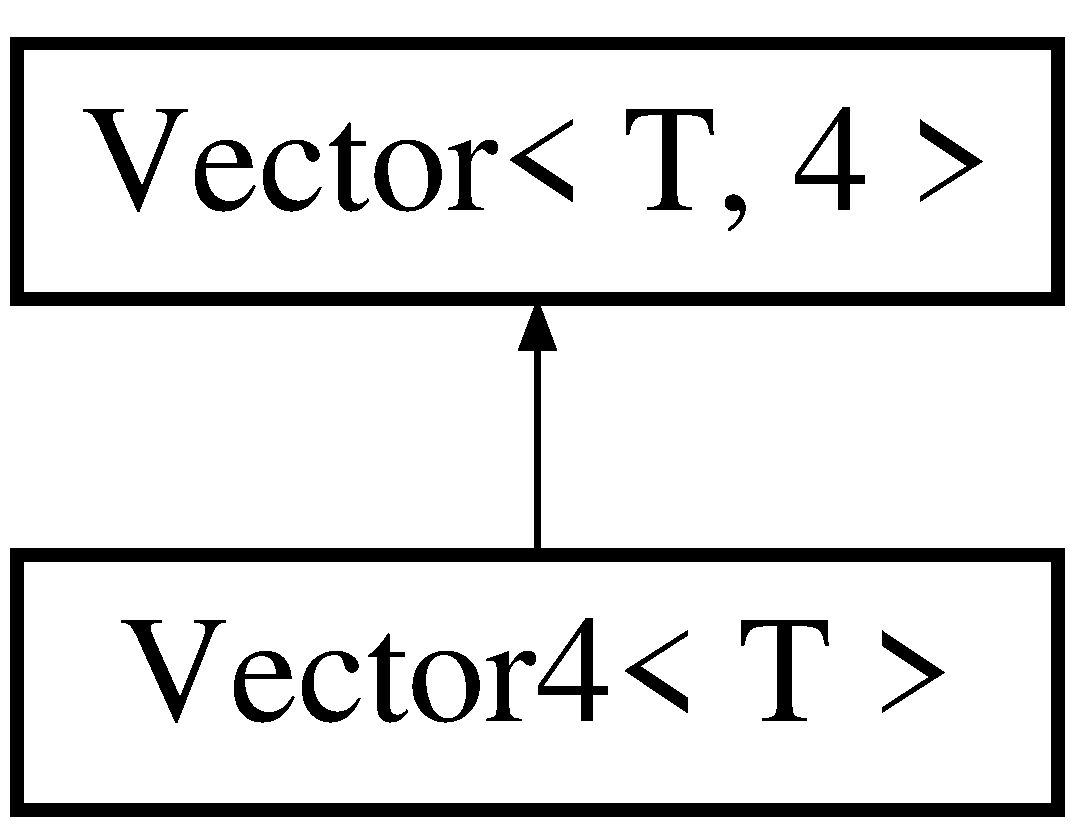
\includegraphics[height=2.000000cm]{class_vector4}
\end{center}
\end{figure}
\subsection*{Public Member Functions}
\begin{DoxyCompactItemize}
\item 
\hyperlink{class_vector4_afdef97d94e5697622b5322637028accf}{Vector4} ()
\item 
\hyperlink{class_vector4_acbf5f4e37a678abcc2fa00e0e633f41a}{Vector4} (const \hyperlink{class_vector}{Vector}$<$ T, 4 $>$ \&r)
\item 
\hyperlink{class_vector4_ad0da88beeb8b4f77e05f9faddc21469b}{Vector4} (T x, T y, T z, T w)
\item 
T \hyperlink{class_vector4_a90e0c7b7b1cc89c1faaba14bcd3f585a}{Get\+X} () const 
\item 
T \hyperlink{class_vector4_a7c178a0068d7ec3a77fb8239052bbe42}{Get\+Y} () const 
\item 
T \hyperlink{class_vector4_ad66bdb268d13fc3b8e9b040dd3c7ef03}{Get\+Z} () const 
\item 
T \hyperlink{class_vector4_a12ee3cad6a9f37ed5f71a1f214d324ec}{Get\+W} () const 
\item 
void \hyperlink{class_vector4_a4ac9438f9f5464db3dff215c773a7290}{Set\+X} (const T \&x)
\item 
void \hyperlink{class_vector4_a0529ac9fdbb27baa288cdf9cbcc0ba80}{Set\+Y} (const T \&y)
\item 
void \hyperlink{class_vector4_aa595f39077a0b28f6a3e4b7054b84aed}{Set\+Z} (const T \&z)
\item 
void \hyperlink{class_vector4_a8fb9f197a3ff3d9c2f46ccac6795ac5c}{Set\+W} (const T \&w)
\item 
void \hyperlink{class_vector4_a2ee3defe0236534fd145fb239dbfbaf4}{Set} (const T \&x, const T \&y, const T \&z, const T \&w)
\end{DoxyCompactItemize}


\subsection{Constructor \& Destructor Documentation}
\hypertarget{class_vector4_afdef97d94e5697622b5322637028accf}{}\index{Vector4@{Vector4}!Vector4@{Vector4}}
\index{Vector4@{Vector4}!Vector4@{Vector4}}
\subsubsection[{Vector4()}]{\setlength{\rightskip}{0pt plus 5cm}template$<$typename T$>$ {\bf Vector4}$<$ T $>$\+::{\bf Vector4} (
\begin{DoxyParamCaption}
{}
\end{DoxyParamCaption}
)\hspace{0.3cm}{\ttfamily [inline]}}\label{class_vector4_afdef97d94e5697622b5322637028accf}
\hypertarget{class_vector4_acbf5f4e37a678abcc2fa00e0e633f41a}{}\index{Vector4@{Vector4}!Vector4@{Vector4}}
\index{Vector4@{Vector4}!Vector4@{Vector4}}
\subsubsection[{Vector4(const Vector$<$ T, 4 $>$ \&r)}]{\setlength{\rightskip}{0pt plus 5cm}template$<$typename T$>$ {\bf Vector4}$<$ T $>$\+::{\bf Vector4} (
\begin{DoxyParamCaption}
\item[{const {\bf Vector}$<$ T, 4 $>$ \&}]{r}
\end{DoxyParamCaption}
)\hspace{0.3cm}{\ttfamily [inline]}}\label{class_vector4_acbf5f4e37a678abcc2fa00e0e633f41a}
\hypertarget{class_vector4_ad0da88beeb8b4f77e05f9faddc21469b}{}\index{Vector4@{Vector4}!Vector4@{Vector4}}
\index{Vector4@{Vector4}!Vector4@{Vector4}}
\subsubsection[{Vector4(\+T x, T y, T z, T w)}]{\setlength{\rightskip}{0pt plus 5cm}template$<$typename T$>$ {\bf Vector4}$<$ T $>$\+::{\bf Vector4} (
\begin{DoxyParamCaption}
\item[{T}]{x, }
\item[{T}]{y, }
\item[{T}]{z, }
\item[{T}]{w}
\end{DoxyParamCaption}
)\hspace{0.3cm}{\ttfamily [inline]}}\label{class_vector4_ad0da88beeb8b4f77e05f9faddc21469b}


\subsection{Member Function Documentation}
\hypertarget{class_vector4_a12ee3cad6a9f37ed5f71a1f214d324ec}{}\index{Vector4@{Vector4}!Get\+W@{Get\+W}}
\index{Get\+W@{Get\+W}!Vector4@{Vector4}}
\subsubsection[{Get\+W() const }]{\setlength{\rightskip}{0pt plus 5cm}template$<$typename T$>$ T {\bf Vector4}$<$ T $>$\+::Get\+W (
\begin{DoxyParamCaption}
{}
\end{DoxyParamCaption}
) const\hspace{0.3cm}{\ttfamily [inline]}}\label{class_vector4_a12ee3cad6a9f37ed5f71a1f214d324ec}
\hypertarget{class_vector4_a90e0c7b7b1cc89c1faaba14bcd3f585a}{}\index{Vector4@{Vector4}!Get\+X@{Get\+X}}
\index{Get\+X@{Get\+X}!Vector4@{Vector4}}
\subsubsection[{Get\+X() const }]{\setlength{\rightskip}{0pt plus 5cm}template$<$typename T$>$ T {\bf Vector4}$<$ T $>$\+::Get\+X (
\begin{DoxyParamCaption}
{}
\end{DoxyParamCaption}
) const\hspace{0.3cm}{\ttfamily [inline]}}\label{class_vector4_a90e0c7b7b1cc89c1faaba14bcd3f585a}
\hypertarget{class_vector4_a7c178a0068d7ec3a77fb8239052bbe42}{}\index{Vector4@{Vector4}!Get\+Y@{Get\+Y}}
\index{Get\+Y@{Get\+Y}!Vector4@{Vector4}}
\subsubsection[{Get\+Y() const }]{\setlength{\rightskip}{0pt plus 5cm}template$<$typename T$>$ T {\bf Vector4}$<$ T $>$\+::Get\+Y (
\begin{DoxyParamCaption}
{}
\end{DoxyParamCaption}
) const\hspace{0.3cm}{\ttfamily [inline]}}\label{class_vector4_a7c178a0068d7ec3a77fb8239052bbe42}
\hypertarget{class_vector4_ad66bdb268d13fc3b8e9b040dd3c7ef03}{}\index{Vector4@{Vector4}!Get\+Z@{Get\+Z}}
\index{Get\+Z@{Get\+Z}!Vector4@{Vector4}}
\subsubsection[{Get\+Z() const }]{\setlength{\rightskip}{0pt plus 5cm}template$<$typename T$>$ T {\bf Vector4}$<$ T $>$\+::Get\+Z (
\begin{DoxyParamCaption}
{}
\end{DoxyParamCaption}
) const\hspace{0.3cm}{\ttfamily [inline]}}\label{class_vector4_ad66bdb268d13fc3b8e9b040dd3c7ef03}
\hypertarget{class_vector4_a2ee3defe0236534fd145fb239dbfbaf4}{}\index{Vector4@{Vector4}!Set@{Set}}
\index{Set@{Set}!Vector4@{Vector4}}
\subsubsection[{Set(const T \&x, const T \&y, const T \&z, const T \&w)}]{\setlength{\rightskip}{0pt plus 5cm}template$<$typename T$>$ void {\bf Vector4}$<$ T $>$\+::Set (
\begin{DoxyParamCaption}
\item[{const T \&}]{x, }
\item[{const T \&}]{y, }
\item[{const T \&}]{z, }
\item[{const T \&}]{w}
\end{DoxyParamCaption}
)\hspace{0.3cm}{\ttfamily [inline]}}\label{class_vector4_a2ee3defe0236534fd145fb239dbfbaf4}
\hypertarget{class_vector4_a8fb9f197a3ff3d9c2f46ccac6795ac5c}{}\index{Vector4@{Vector4}!Set\+W@{Set\+W}}
\index{Set\+W@{Set\+W}!Vector4@{Vector4}}
\subsubsection[{Set\+W(const T \&w)}]{\setlength{\rightskip}{0pt plus 5cm}template$<$typename T$>$ void {\bf Vector4}$<$ T $>$\+::Set\+W (
\begin{DoxyParamCaption}
\item[{const T \&}]{w}
\end{DoxyParamCaption}
)\hspace{0.3cm}{\ttfamily [inline]}}\label{class_vector4_a8fb9f197a3ff3d9c2f46ccac6795ac5c}
\hypertarget{class_vector4_a4ac9438f9f5464db3dff215c773a7290}{}\index{Vector4@{Vector4}!Set\+X@{Set\+X}}
\index{Set\+X@{Set\+X}!Vector4@{Vector4}}
\subsubsection[{Set\+X(const T \&x)}]{\setlength{\rightskip}{0pt plus 5cm}template$<$typename T$>$ void {\bf Vector4}$<$ T $>$\+::Set\+X (
\begin{DoxyParamCaption}
\item[{const T \&}]{x}
\end{DoxyParamCaption}
)\hspace{0.3cm}{\ttfamily [inline]}}\label{class_vector4_a4ac9438f9f5464db3dff215c773a7290}
\hypertarget{class_vector4_a0529ac9fdbb27baa288cdf9cbcc0ba80}{}\index{Vector4@{Vector4}!Set\+Y@{Set\+Y}}
\index{Set\+Y@{Set\+Y}!Vector4@{Vector4}}
\subsubsection[{Set\+Y(const T \&y)}]{\setlength{\rightskip}{0pt plus 5cm}template$<$typename T$>$ void {\bf Vector4}$<$ T $>$\+::Set\+Y (
\begin{DoxyParamCaption}
\item[{const T \&}]{y}
\end{DoxyParamCaption}
)\hspace{0.3cm}{\ttfamily [inline]}}\label{class_vector4_a0529ac9fdbb27baa288cdf9cbcc0ba80}
\hypertarget{class_vector4_aa595f39077a0b28f6a3e4b7054b84aed}{}\index{Vector4@{Vector4}!Set\+Z@{Set\+Z}}
\index{Set\+Z@{Set\+Z}!Vector4@{Vector4}}
\subsubsection[{Set\+Z(const T \&z)}]{\setlength{\rightskip}{0pt plus 5cm}template$<$typename T$>$ void {\bf Vector4}$<$ T $>$\+::Set\+Z (
\begin{DoxyParamCaption}
\item[{const T \&}]{z}
\end{DoxyParamCaption}
)\hspace{0.3cm}{\ttfamily [inline]}}\label{class_vector4_aa595f39077a0b28f6a3e4b7054b84aed}


The documentation for this class was generated from the following file\+:\begin{DoxyCompactItemize}
\item 
F\+:/\+Fusion3\+D\+\_\+work/src/core/\hyperlink{math3d_8h}{math3d.\+h}\end{DoxyCompactItemize}

\hypertarget{class_window}{}\section{Window Class Reference}
\label{class_window}\index{Window@{Window}}


{\ttfamily \#include $<$window.\+h$>$}

\subsection*{Public Member Functions}
\begin{DoxyCompactItemize}
\item 
\hyperlink{class_window_a2bf7954f0cf38a7fc4c4742e4a91a190}{Window} (int width, int height, const std\+::string \&title)
\item 
virtual \hyperlink{class_window_a245d821e6016fa1f6970ccbbedd635f6}{$\sim$\+Window} ()
\item 
void \hyperlink{class_window_ab8d28dce3166c70eb5744466460795df}{Update} ()
\item 
void \hyperlink{class_window_abe1b83eda6980f2b9964aab08b5310ed}{Swap\+Buffers} ()
\item 
void \hyperlink{class_window_a7b9db9583287699589b2cd8414eb8ca3}{Bind\+As\+Render\+Target} () const 
\item 
bool \hyperlink{class_window_ad8d9c297161e3221fdfe8e1b22d82d16}{Is\+Close\+Requested} () const 
\item 
int \hyperlink{class_window_a002e19bc6ca085926d13cf7b97bb3cd3}{Get\+Width} () const 
\item 
int \hyperlink{class_window_a75f6cc315ae3ea6794e640e610d0fb44}{Get\+Height} () const 
\item 
float \hyperlink{class_window_a8cbbffba60d9268b485e713726290c84}{Get\+Aspect} () const 
\item 
const std\+::string \& \hyperlink{class_window_ab6279d2fd6158716efa5b75fed4670d2}{Get\+Title} () const 
\item 
\hyperlink{math3d_8h_a9f3739462b0605dcb64299fa289b6afe}{Vector2f} \hyperlink{class_window_a0f4737f348e84b915dfdbcbba19876c7}{Get\+Center} () const 
\item 
S\+D\+L\+\_\+\+Window $\ast$ \hyperlink{class_window_ae9b9dadb24a237aa3b6ce43e03d0f592}{Get\+S\+D\+L\+Window} ()
\item 
const \hyperlink{class_input}{Input} \& \hyperlink{class_window_a0e893bddb6d546a8f2966df21e44249c}{Get\+Input} () const 
\item 
void \hyperlink{class_window_a5aca5526280a2f95f42c732a407a6129}{Set\+Full\+Screen} (bool value)
\end{DoxyCompactItemize}


\subsection{Constructor \& Destructor Documentation}
\hypertarget{class_window_a2bf7954f0cf38a7fc4c4742e4a91a190}{}\index{Window@{Window}!Window@{Window}}
\index{Window@{Window}!Window@{Window}}
\subsubsection[{Window(int width, int height, const std\+::string \&title)}]{\setlength{\rightskip}{0pt plus 5cm}Window\+::\+Window (
\begin{DoxyParamCaption}
\item[{int}]{width, }
\item[{int}]{height, }
\item[{const std\+::string \&}]{title}
\end{DoxyParamCaption}
)}\label{class_window_a2bf7954f0cf38a7fc4c4742e4a91a190}
\hypertarget{class_window_a245d821e6016fa1f6970ccbbedd635f6}{}\index{Window@{Window}!````~Window@{$\sim$\+Window}}
\index{````~Window@{$\sim$\+Window}!Window@{Window}}
\subsubsection[{$\sim$\+Window()}]{\setlength{\rightskip}{0pt plus 5cm}Window\+::$\sim$\+Window (
\begin{DoxyParamCaption}
{}
\end{DoxyParamCaption}
)\hspace{0.3cm}{\ttfamily [virtual]}}\label{class_window_a245d821e6016fa1f6970ccbbedd635f6}


\subsection{Member Function Documentation}
\hypertarget{class_window_a7b9db9583287699589b2cd8414eb8ca3}{}\index{Window@{Window}!Bind\+As\+Render\+Target@{Bind\+As\+Render\+Target}}
\index{Bind\+As\+Render\+Target@{Bind\+As\+Render\+Target}!Window@{Window}}
\subsubsection[{Bind\+As\+Render\+Target() const }]{\setlength{\rightskip}{0pt plus 5cm}void Window\+::\+Bind\+As\+Render\+Target (
\begin{DoxyParamCaption}
{}
\end{DoxyParamCaption}
) const}\label{class_window_a7b9db9583287699589b2cd8414eb8ca3}
\hypertarget{class_window_a8cbbffba60d9268b485e713726290c84}{}\index{Window@{Window}!Get\+Aspect@{Get\+Aspect}}
\index{Get\+Aspect@{Get\+Aspect}!Window@{Window}}
\subsubsection[{Get\+Aspect() const }]{\setlength{\rightskip}{0pt plus 5cm}float Window\+::\+Get\+Aspect (
\begin{DoxyParamCaption}
{}
\end{DoxyParamCaption}
) const\hspace{0.3cm}{\ttfamily [inline]}}\label{class_window_a8cbbffba60d9268b485e713726290c84}
\hypertarget{class_window_a0f4737f348e84b915dfdbcbba19876c7}{}\index{Window@{Window}!Get\+Center@{Get\+Center}}
\index{Get\+Center@{Get\+Center}!Window@{Window}}
\subsubsection[{Get\+Center() const }]{\setlength{\rightskip}{0pt plus 5cm}{\bf Vector2f} Window\+::\+Get\+Center (
\begin{DoxyParamCaption}
{}
\end{DoxyParamCaption}
) const\hspace{0.3cm}{\ttfamily [inline]}}\label{class_window_a0f4737f348e84b915dfdbcbba19876c7}
\hypertarget{class_window_a75f6cc315ae3ea6794e640e610d0fb44}{}\index{Window@{Window}!Get\+Height@{Get\+Height}}
\index{Get\+Height@{Get\+Height}!Window@{Window}}
\subsubsection[{Get\+Height() const }]{\setlength{\rightskip}{0pt plus 5cm}int Window\+::\+Get\+Height (
\begin{DoxyParamCaption}
{}
\end{DoxyParamCaption}
) const\hspace{0.3cm}{\ttfamily [inline]}}\label{class_window_a75f6cc315ae3ea6794e640e610d0fb44}
\hypertarget{class_window_a0e893bddb6d546a8f2966df21e44249c}{}\index{Window@{Window}!Get\+Input@{Get\+Input}}
\index{Get\+Input@{Get\+Input}!Window@{Window}}
\subsubsection[{Get\+Input() const }]{\setlength{\rightskip}{0pt plus 5cm}const {\bf Input}\& Window\+::\+Get\+Input (
\begin{DoxyParamCaption}
{}
\end{DoxyParamCaption}
) const\hspace{0.3cm}{\ttfamily [inline]}}\label{class_window_a0e893bddb6d546a8f2966df21e44249c}
\hypertarget{class_window_ae9b9dadb24a237aa3b6ce43e03d0f592}{}\index{Window@{Window}!Get\+S\+D\+L\+Window@{Get\+S\+D\+L\+Window}}
\index{Get\+S\+D\+L\+Window@{Get\+S\+D\+L\+Window}!Window@{Window}}
\subsubsection[{Get\+S\+D\+L\+Window()}]{\setlength{\rightskip}{0pt plus 5cm}S\+D\+L\+\_\+\+Window$\ast$ Window\+::\+Get\+S\+D\+L\+Window (
\begin{DoxyParamCaption}
{}
\end{DoxyParamCaption}
)\hspace{0.3cm}{\ttfamily [inline]}}\label{class_window_ae9b9dadb24a237aa3b6ce43e03d0f592}
\hypertarget{class_window_ab6279d2fd6158716efa5b75fed4670d2}{}\index{Window@{Window}!Get\+Title@{Get\+Title}}
\index{Get\+Title@{Get\+Title}!Window@{Window}}
\subsubsection[{Get\+Title() const }]{\setlength{\rightskip}{0pt plus 5cm}const std\+::string\& Window\+::\+Get\+Title (
\begin{DoxyParamCaption}
{}
\end{DoxyParamCaption}
) const\hspace{0.3cm}{\ttfamily [inline]}}\label{class_window_ab6279d2fd6158716efa5b75fed4670d2}
\hypertarget{class_window_a002e19bc6ca085926d13cf7b97bb3cd3}{}\index{Window@{Window}!Get\+Width@{Get\+Width}}
\index{Get\+Width@{Get\+Width}!Window@{Window}}
\subsubsection[{Get\+Width() const }]{\setlength{\rightskip}{0pt plus 5cm}int Window\+::\+Get\+Width (
\begin{DoxyParamCaption}
{}
\end{DoxyParamCaption}
) const\hspace{0.3cm}{\ttfamily [inline]}}\label{class_window_a002e19bc6ca085926d13cf7b97bb3cd3}
\hypertarget{class_window_ad8d9c297161e3221fdfe8e1b22d82d16}{}\index{Window@{Window}!Is\+Close\+Requested@{Is\+Close\+Requested}}
\index{Is\+Close\+Requested@{Is\+Close\+Requested}!Window@{Window}}
\subsubsection[{Is\+Close\+Requested() const }]{\setlength{\rightskip}{0pt plus 5cm}bool Window\+::\+Is\+Close\+Requested (
\begin{DoxyParamCaption}
{}
\end{DoxyParamCaption}
) const\hspace{0.3cm}{\ttfamily [inline]}}\label{class_window_ad8d9c297161e3221fdfe8e1b22d82d16}
\hypertarget{class_window_a5aca5526280a2f95f42c732a407a6129}{}\index{Window@{Window}!Set\+Full\+Screen@{Set\+Full\+Screen}}
\index{Set\+Full\+Screen@{Set\+Full\+Screen}!Window@{Window}}
\subsubsection[{Set\+Full\+Screen(bool value)}]{\setlength{\rightskip}{0pt plus 5cm}void Window\+::\+Set\+Full\+Screen (
\begin{DoxyParamCaption}
\item[{bool}]{value}
\end{DoxyParamCaption}
)}\label{class_window_a5aca5526280a2f95f42c732a407a6129}
\hypertarget{class_window_abe1b83eda6980f2b9964aab08b5310ed}{}\index{Window@{Window}!Swap\+Buffers@{Swap\+Buffers}}
\index{Swap\+Buffers@{Swap\+Buffers}!Window@{Window}}
\subsubsection[{Swap\+Buffers()}]{\setlength{\rightskip}{0pt plus 5cm}void Window\+::\+Swap\+Buffers (
\begin{DoxyParamCaption}
{}
\end{DoxyParamCaption}
)}\label{class_window_abe1b83eda6980f2b9964aab08b5310ed}
\hypertarget{class_window_ab8d28dce3166c70eb5744466460795df}{}\index{Window@{Window}!Update@{Update}}
\index{Update@{Update}!Window@{Window}}
\subsubsection[{Update()}]{\setlength{\rightskip}{0pt plus 5cm}void Window\+::\+Update (
\begin{DoxyParamCaption}
{}
\end{DoxyParamCaption}
)}\label{class_window_ab8d28dce3166c70eb5744466460795df}


The documentation for this class was generated from the following files\+:\begin{DoxyCompactItemize}
\item 
F\+:/\+Fusion3\+D\+\_\+work/src/rendering/\hyperlink{window_8h}{window.\+h}\item 
F\+:/\+Fusion3\+D\+\_\+work/src/rendering/\hyperlink{window_8cpp}{window.\+cpp}\end{DoxyCompactItemize}

\hypertarget{structzbuf}{}\section{zbuf Struct Reference}
\label{structzbuf}\index{zbuf@{zbuf}}
\subsection*{Public Attributes}
\begin{DoxyCompactItemize}
\item 
\hyperlink{stb__image_8c_adde6aaee8457bee49c2a92621fe22b79}{uint8} $\ast$ \hyperlink{structzbuf_a7080eb91dcc67e1dfe818d08e6f22c4e}{zbuffer}
\item 
\hyperlink{stb__image_8c_adde6aaee8457bee49c2a92621fe22b79}{uint8} $\ast$ \hyperlink{structzbuf_af030baa17bebedd18272678da17a33f4}{zbuffer\+\_\+end}
\item 
int \hyperlink{structzbuf_acd069cdb4100884a732ad2794edbbdff}{num\+\_\+bits}
\item 
\hyperlink{stb__image_8c_a1134b580f8da4de94ca6b1de4d37975e}{uint32} \hyperlink{structzbuf_a3bb8244d7be17801079c5a8587182edb}{code\+\_\+buffer}
\item 
char $\ast$ \hyperlink{structzbuf_aaf137c25fa5b9fb14e92354da4203c38}{zout}
\item 
char $\ast$ \hyperlink{structzbuf_af31571e8d74c78c9bb18d92205150b28}{zout\+\_\+start}
\item 
char $\ast$ \hyperlink{structzbuf_af07c0b7b7227f670ee1413bc0dcab791}{zout\+\_\+end}
\item 
int \hyperlink{structzbuf_ae662f24e0973ca19b543e64647a6bfb6}{z\+\_\+expandable}
\item 
\hyperlink{structzhuffman}{zhuffman} \hyperlink{structzbuf_a5906bdbe9dfb565339acac51af9efe89}{z\+\_\+length}
\item 
\hyperlink{structzhuffman}{zhuffman} \hyperlink{structzbuf_ae7d9588b2548708e14f3c6ad89bf26b5}{z\+\_\+distance}
\end{DoxyCompactItemize}


\subsection{Member Data Documentation}
\hypertarget{structzbuf_a3bb8244d7be17801079c5a8587182edb}{}\index{zbuf@{zbuf}!code\+\_\+buffer@{code\+\_\+buffer}}
\index{code\+\_\+buffer@{code\+\_\+buffer}!zbuf@{zbuf}}
\subsubsection[{code\+\_\+buffer}]{\setlength{\rightskip}{0pt plus 5cm}{\bf uint32} zbuf\+::code\+\_\+buffer}\label{structzbuf_a3bb8244d7be17801079c5a8587182edb}
\hypertarget{structzbuf_acd069cdb4100884a732ad2794edbbdff}{}\index{zbuf@{zbuf}!num\+\_\+bits@{num\+\_\+bits}}
\index{num\+\_\+bits@{num\+\_\+bits}!zbuf@{zbuf}}
\subsubsection[{num\+\_\+bits}]{\setlength{\rightskip}{0pt plus 5cm}int zbuf\+::num\+\_\+bits}\label{structzbuf_acd069cdb4100884a732ad2794edbbdff}
\hypertarget{structzbuf_ae7d9588b2548708e14f3c6ad89bf26b5}{}\index{zbuf@{zbuf}!z\+\_\+distance@{z\+\_\+distance}}
\index{z\+\_\+distance@{z\+\_\+distance}!zbuf@{zbuf}}
\subsubsection[{z\+\_\+distance}]{\setlength{\rightskip}{0pt plus 5cm}{\bf zhuffman} zbuf\+::z\+\_\+distance}\label{structzbuf_ae7d9588b2548708e14f3c6ad89bf26b5}
\hypertarget{structzbuf_ae662f24e0973ca19b543e64647a6bfb6}{}\index{zbuf@{zbuf}!z\+\_\+expandable@{z\+\_\+expandable}}
\index{z\+\_\+expandable@{z\+\_\+expandable}!zbuf@{zbuf}}
\subsubsection[{z\+\_\+expandable}]{\setlength{\rightskip}{0pt plus 5cm}int zbuf\+::z\+\_\+expandable}\label{structzbuf_ae662f24e0973ca19b543e64647a6bfb6}
\hypertarget{structzbuf_a5906bdbe9dfb565339acac51af9efe89}{}\index{zbuf@{zbuf}!z\+\_\+length@{z\+\_\+length}}
\index{z\+\_\+length@{z\+\_\+length}!zbuf@{zbuf}}
\subsubsection[{z\+\_\+length}]{\setlength{\rightskip}{0pt plus 5cm}{\bf zhuffman} zbuf\+::z\+\_\+length}\label{structzbuf_a5906bdbe9dfb565339acac51af9efe89}
\hypertarget{structzbuf_a7080eb91dcc67e1dfe818d08e6f22c4e}{}\index{zbuf@{zbuf}!zbuffer@{zbuffer}}
\index{zbuffer@{zbuffer}!zbuf@{zbuf}}
\subsubsection[{zbuffer}]{\setlength{\rightskip}{0pt plus 5cm}{\bf uint8}$\ast$ zbuf\+::zbuffer}\label{structzbuf_a7080eb91dcc67e1dfe818d08e6f22c4e}
\hypertarget{structzbuf_af030baa17bebedd18272678da17a33f4}{}\index{zbuf@{zbuf}!zbuffer\+\_\+end@{zbuffer\+\_\+end}}
\index{zbuffer\+\_\+end@{zbuffer\+\_\+end}!zbuf@{zbuf}}
\subsubsection[{zbuffer\+\_\+end}]{\setlength{\rightskip}{0pt plus 5cm}{\bf uint8} $\ast$ zbuf\+::zbuffer\+\_\+end}\label{structzbuf_af030baa17bebedd18272678da17a33f4}
\hypertarget{structzbuf_aaf137c25fa5b9fb14e92354da4203c38}{}\index{zbuf@{zbuf}!zout@{zout}}
\index{zout@{zout}!zbuf@{zbuf}}
\subsubsection[{zout}]{\setlength{\rightskip}{0pt plus 5cm}char$\ast$ zbuf\+::zout}\label{structzbuf_aaf137c25fa5b9fb14e92354da4203c38}
\hypertarget{structzbuf_af07c0b7b7227f670ee1413bc0dcab791}{}\index{zbuf@{zbuf}!zout\+\_\+end@{zout\+\_\+end}}
\index{zout\+\_\+end@{zout\+\_\+end}!zbuf@{zbuf}}
\subsubsection[{zout\+\_\+end}]{\setlength{\rightskip}{0pt plus 5cm}char$\ast$ zbuf\+::zout\+\_\+end}\label{structzbuf_af07c0b7b7227f670ee1413bc0dcab791}
\hypertarget{structzbuf_af31571e8d74c78c9bb18d92205150b28}{}\index{zbuf@{zbuf}!zout\+\_\+start@{zout\+\_\+start}}
\index{zout\+\_\+start@{zout\+\_\+start}!zbuf@{zbuf}}
\subsubsection[{zout\+\_\+start}]{\setlength{\rightskip}{0pt plus 5cm}char$\ast$ zbuf\+::zout\+\_\+start}\label{structzbuf_af31571e8d74c78c9bb18d92205150b28}


The documentation for this struct was generated from the following file\+:\begin{DoxyCompactItemize}
\item 
F\+:/\+Fusion3\+D\+\_\+work/src/static\+Libs/\hyperlink{stb__image_8c}{stb\+\_\+image.\+c}\end{DoxyCompactItemize}

\hypertarget{structzhuffman}{}\section{zhuffman Struct Reference}
\label{structzhuffman}\index{zhuffman@{zhuffman}}
\subsection*{Public Attributes}
\begin{DoxyCompactItemize}
\item 
\hyperlink{stb__image_8c_a05f6b0ae8f6a6e135b0e290c25fe0e4e}{uint16} \hyperlink{structzhuffman_a12d5f92a121b65680e5f0b4027d00c96}{fast} \mbox{[}1$<$$<$ \hyperlink{stb__image_8c_a37d8564ae0a820fb44b1a751c702e33a}{Z\+F\+A\+S\+T\+\_\+\+B\+I\+T\+S}\mbox{]}
\item 
\hyperlink{stb__image_8c_a05f6b0ae8f6a6e135b0e290c25fe0e4e}{uint16} \hyperlink{structzhuffman_a81f5ae5bd31b40439955de6154572917}{firstcode} \mbox{[}16\mbox{]}
\item 
int \hyperlink{structzhuffman_ac7dd4a2bf01a6e27933dd1cf6b0cc762}{maxcode} \mbox{[}17\mbox{]}
\item 
\hyperlink{stb__image_8c_a05f6b0ae8f6a6e135b0e290c25fe0e4e}{uint16} \hyperlink{structzhuffman_afbdb21fd99f413fc8f9e58243552fe95}{firstsymbol} \mbox{[}16\mbox{]}
\item 
\hyperlink{stb__image_8c_adde6aaee8457bee49c2a92621fe22b79}{uint8} \hyperlink{structzhuffman_a46ce4d4a4d7fc41c2560616f6696e9b9}{size} \mbox{[}288\mbox{]}
\item 
\hyperlink{stb__image_8c_a05f6b0ae8f6a6e135b0e290c25fe0e4e}{uint16} \hyperlink{structzhuffman_acc395b638b700b944c329d71a8b82084}{value} \mbox{[}288\mbox{]}
\end{DoxyCompactItemize}


\subsection{Member Data Documentation}
\hypertarget{structzhuffman_a12d5f92a121b65680e5f0b4027d00c96}{}\index{zhuffman@{zhuffman}!fast@{fast}}
\index{fast@{fast}!zhuffman@{zhuffman}}
\subsubsection[{fast}]{\setlength{\rightskip}{0pt plus 5cm}{\bf uint16} zhuffman\+::fast\mbox{[}1$<$$<$ {\bf Z\+F\+A\+S\+T\+\_\+\+B\+I\+T\+S}\mbox{]}}\label{structzhuffman_a12d5f92a121b65680e5f0b4027d00c96}
\hypertarget{structzhuffman_a81f5ae5bd31b40439955de6154572917}{}\index{zhuffman@{zhuffman}!firstcode@{firstcode}}
\index{firstcode@{firstcode}!zhuffman@{zhuffman}}
\subsubsection[{firstcode}]{\setlength{\rightskip}{0pt plus 5cm}{\bf uint16} zhuffman\+::firstcode\mbox{[}16\mbox{]}}\label{structzhuffman_a81f5ae5bd31b40439955de6154572917}
\hypertarget{structzhuffman_afbdb21fd99f413fc8f9e58243552fe95}{}\index{zhuffman@{zhuffman}!firstsymbol@{firstsymbol}}
\index{firstsymbol@{firstsymbol}!zhuffman@{zhuffman}}
\subsubsection[{firstsymbol}]{\setlength{\rightskip}{0pt plus 5cm}{\bf uint16} zhuffman\+::firstsymbol\mbox{[}16\mbox{]}}\label{structzhuffman_afbdb21fd99f413fc8f9e58243552fe95}
\hypertarget{structzhuffman_ac7dd4a2bf01a6e27933dd1cf6b0cc762}{}\index{zhuffman@{zhuffman}!maxcode@{maxcode}}
\index{maxcode@{maxcode}!zhuffman@{zhuffman}}
\subsubsection[{maxcode}]{\setlength{\rightskip}{0pt plus 5cm}int zhuffman\+::maxcode\mbox{[}17\mbox{]}}\label{structzhuffman_ac7dd4a2bf01a6e27933dd1cf6b0cc762}
\hypertarget{structzhuffman_a46ce4d4a4d7fc41c2560616f6696e9b9}{}\index{zhuffman@{zhuffman}!size@{size}}
\index{size@{size}!zhuffman@{zhuffman}}
\subsubsection[{size}]{\setlength{\rightskip}{0pt plus 5cm}{\bf uint8} zhuffman\+::size\mbox{[}288\mbox{]}}\label{structzhuffman_a46ce4d4a4d7fc41c2560616f6696e9b9}
\hypertarget{structzhuffman_acc395b638b700b944c329d71a8b82084}{}\index{zhuffman@{zhuffman}!value@{value}}
\index{value@{value}!zhuffman@{zhuffman}}
\subsubsection[{value}]{\setlength{\rightskip}{0pt plus 5cm}{\bf uint16} zhuffman\+::value\mbox{[}288\mbox{]}}\label{structzhuffman_acc395b638b700b944c329d71a8b82084}


The documentation for this struct was generated from the following file\+:\begin{DoxyCompactItemize}
\item 
F\+:/\+Fusion3\+D\+\_\+work/src/static\+Libs/\hyperlink{stb__image_8c}{stb\+\_\+image.\+c}\end{DoxyCompactItemize}

\chapter{File Documentation}
\hypertarget{3_d_engine_8h}{}\section{F\+:/\+Fusion3\+D\+\_\+work/src/3\+D\+Engine.h File Reference}
\label{3_d_engine_8h}\index{F\+:/\+Fusion3\+D\+\_\+work/src/3\+D\+Engine.\+h@{F\+:/\+Fusion3\+D\+\_\+work/src/3\+D\+Engine.\+h}}
{\ttfamily \#include \char`\"{}bt\+Bullet\+Dynamics\+Common.\+h\char`\"{}}\\*
{\ttfamily \#include \char`\"{}rendering/mesh.\+h\char`\"{}}\\*
{\ttfamily \#include \char`\"{}rendering/shader.\+h\char`\"{}}\\*
{\ttfamily \#include \char`\"{}core/transform.\+h\char`\"{}}\\*
{\ttfamily \#include \char`\"{}rendering/camera.\+h\char`\"{}}\\*
{\ttfamily \#include \char`\"{}rendering/lighting.\+h\char`\"{}}\\*
{\ttfamily \#include \char`\"{}core/entity.\+h\char`\"{}}\\*
{\ttfamily \#include \char`\"{}components/mesh\+Renderer.\+h\char`\"{}}\\*
{\ttfamily \#include \char`\"{}components/program\+Component.\+h\char`\"{}}\\*
{\ttfamily \#include \char`\"{}rendering/window.\+h\char`\"{}}\\*
{\ttfamily \#include \char`\"{}core/core\+Engine.\+h\char`\"{}}\\*
{\ttfamily \#include \char`\"{}core/game.\+h\char`\"{}}\\*
\subsection*{Macros}
\begin{DoxyCompactItemize}
\item 
\#define \hyperlink{3_d_engine_8h_a75c828ed6c02fcd44084e67a032e422c}{F\+O\+R\+E\+V\+E\+R}~for (;;)
\item 
\#define \hyperlink{3_d_engine_8h_abfc4fe4d7e71ae79cd50152d0f286333}{F\+O\+R}(p,  q,  z)~for (size\+\_\+t z = p; z $<$ q; ++z)
\item 
\#define \hyperlink{3_d_engine_8h_ab76d198e4b62f15516638896c1f9dfa8}{D\+F\+O\+R}(p,  q,  z)~for (size\+\_\+t z = q; z $>$ p; -\/-\/z)
\item 
\#define \hyperlink{3_d_engine_8h_aac699a3288732fdc5f67c48c6cea8aa9}{P\+R\+I\+N\+T}(p)~std\+::cout $<$$<$ p $<$$<$ std\+::endl
\item 
\#define \hyperlink{3_d_engine_8h_a8f7bd5242b15da973671df869db5fe85}{S\+T\+R\+I\+N\+G}(s)~\#s
\end{DoxyCompactItemize}


\subsection{Macro Definition Documentation}
\hypertarget{3_d_engine_8h_ab76d198e4b62f15516638896c1f9dfa8}{}\index{3\+D\+Engine.\+h@{3\+D\+Engine.\+h}!D\+F\+O\+R@{D\+F\+O\+R}}
\index{D\+F\+O\+R@{D\+F\+O\+R}!3\+D\+Engine.\+h@{3\+D\+Engine.\+h}}
\subsubsection[{D\+F\+O\+R}]{\setlength{\rightskip}{0pt plus 5cm}\#define D\+F\+O\+R(
\begin{DoxyParamCaption}
\item[{}]{p, }
\item[{}]{q, }
\item[{}]{z}
\end{DoxyParamCaption}
)~for (size\+\_\+t z = q; z $>$ p; -\/-\/z)}\label{3_d_engine_8h_ab76d198e4b62f15516638896c1f9dfa8}
\hypertarget{3_d_engine_8h_abfc4fe4d7e71ae79cd50152d0f286333}{}\index{3\+D\+Engine.\+h@{3\+D\+Engine.\+h}!F\+O\+R@{F\+O\+R}}
\index{F\+O\+R@{F\+O\+R}!3\+D\+Engine.\+h@{3\+D\+Engine.\+h}}
\subsubsection[{F\+O\+R}]{\setlength{\rightskip}{0pt plus 5cm}\#define F\+O\+R(
\begin{DoxyParamCaption}
\item[{}]{p, }
\item[{}]{q, }
\item[{}]{z}
\end{DoxyParamCaption}
)~for (size\+\_\+t z = p; z $<$ q; ++z)}\label{3_d_engine_8h_abfc4fe4d7e71ae79cd50152d0f286333}
\hypertarget{3_d_engine_8h_a75c828ed6c02fcd44084e67a032e422c}{}\index{3\+D\+Engine.\+h@{3\+D\+Engine.\+h}!F\+O\+R\+E\+V\+E\+R@{F\+O\+R\+E\+V\+E\+R}}
\index{F\+O\+R\+E\+V\+E\+R@{F\+O\+R\+E\+V\+E\+R}!3\+D\+Engine.\+h@{3\+D\+Engine.\+h}}
\subsubsection[{F\+O\+R\+E\+V\+E\+R}]{\setlength{\rightskip}{0pt plus 5cm}\#define F\+O\+R\+E\+V\+E\+R~for (;;)}\label{3_d_engine_8h_a75c828ed6c02fcd44084e67a032e422c}
\hypertarget{3_d_engine_8h_aac699a3288732fdc5f67c48c6cea8aa9}{}\index{3\+D\+Engine.\+h@{3\+D\+Engine.\+h}!P\+R\+I\+N\+T@{P\+R\+I\+N\+T}}
\index{P\+R\+I\+N\+T@{P\+R\+I\+N\+T}!3\+D\+Engine.\+h@{3\+D\+Engine.\+h}}
\subsubsection[{P\+R\+I\+N\+T}]{\setlength{\rightskip}{0pt plus 5cm}\#define P\+R\+I\+N\+T(
\begin{DoxyParamCaption}
\item[{}]{p}
\end{DoxyParamCaption}
)~std\+::cout $<$$<$ p $<$$<$ std\+::endl}\label{3_d_engine_8h_aac699a3288732fdc5f67c48c6cea8aa9}
\hypertarget{3_d_engine_8h_a8f7bd5242b15da973671df869db5fe85}{}\index{3\+D\+Engine.\+h@{3\+D\+Engine.\+h}!S\+T\+R\+I\+N\+G@{S\+T\+R\+I\+N\+G}}
\index{S\+T\+R\+I\+N\+G@{S\+T\+R\+I\+N\+G}!3\+D\+Engine.\+h@{3\+D\+Engine.\+h}}
\subsubsection[{S\+T\+R\+I\+N\+G}]{\setlength{\rightskip}{0pt plus 5cm}\#define S\+T\+R\+I\+N\+G(
\begin{DoxyParamCaption}
\item[{}]{s}
\end{DoxyParamCaption}
)~\#s}\label{3_d_engine_8h_a8f7bd5242b15da973671df869db5fe85}

\hypertarget{decal_renderer_8h}{}\section{F\+:/\+Fusion3\+D\+\_\+work/src/components/decal\+Renderer.h File Reference}
\label{decal_renderer_8h}\index{F\+:/\+Fusion3\+D\+\_\+work/src/components/decal\+Renderer.\+h@{F\+:/\+Fusion3\+D\+\_\+work/src/components/decal\+Renderer.\+h}}
{\ttfamily \#include \char`\"{}../core/entity\+Component.\+h\char`\"{}}\\*
{\ttfamily \#include \char`\"{}../rendering/mesh.\+h\char`\"{}}\\*
\subsection*{Functions}
\begin{DoxyCompactItemize}
\item 
\hyperlink{decal_renderer_8h_abcbacd8ba60968b6b629407fa4b6a5c8}{Decal\+Renderer} (\hyperlink{class_material}{Material} $\ast$material)
\item 
virtual void \hyperlink{decal_renderer_8h_a3e0b39e1326de703012f81ac2be7feba}{Init} ()
\item 
virtual void \hyperlink{decal_renderer_8h_a0800e8d38574f7f4a6bc5634bbe01a10}{Render} (const \hyperlink{class_shader}{Shader} \&shader, const \hyperlink{class_rendering_engine}{Rendering\+Engine} \&rendering\+Engine, const \hyperlink{class_camera}{Camera} \&camera) const 
\item 
\hyperlink{class_entity_component}{Entity\+Component} $\ast$ \hyperlink{decal_renderer_8h_ab61d70f8e65639b1757dcea484e1678d}{Set\+Visible} (bool visible)
\item 
bool \hyperlink{decal_renderer_8h_afcd62a638f43f1f9c3a507b923a2dffd}{Is\+Visible} ()
\end{DoxyCompactItemize}
\subsection*{Variables}
\begin{DoxyCompactItemize}
\item 
\hyperlink{class_material}{Material} $\ast$ \hyperlink{decal_renderer_8h_a84b5cec9eabf98fd95a98bd0d1fc4168}{m\+\_\+material}
\item 
bool \hyperlink{decal_renderer_8h_adf7ad65deb2fca5eab8d0674602fe3c4}{m\+\_\+visible}
\end{DoxyCompactItemize}


\subsection{Function Documentation}
\hypertarget{decal_renderer_8h_abcbacd8ba60968b6b629407fa4b6a5c8}{}\index{decal\+Renderer.\+h@{decal\+Renderer.\+h}!Decal\+Renderer@{Decal\+Renderer}}
\index{Decal\+Renderer@{Decal\+Renderer}!decal\+Renderer.\+h@{decal\+Renderer.\+h}}
\subsubsection[{Decal\+Renderer(\+Material $\ast$material)}]{\setlength{\rightskip}{0pt plus 5cm}Decal\+Renderer (
\begin{DoxyParamCaption}
\item[{{\bf Material} $\ast$}]{material}
\end{DoxyParamCaption}
)}\label{decal_renderer_8h_abcbacd8ba60968b6b629407fa4b6a5c8}
\hypertarget{decal_renderer_8h_a3e0b39e1326de703012f81ac2be7feba}{}\index{decal\+Renderer.\+h@{decal\+Renderer.\+h}!Init@{Init}}
\index{Init@{Init}!decal\+Renderer.\+h@{decal\+Renderer.\+h}}
\subsubsection[{Init()}]{\setlength{\rightskip}{0pt plus 5cm}virtual void Init (
\begin{DoxyParamCaption}
{}
\end{DoxyParamCaption}
)\hspace{0.3cm}{\ttfamily [virtual]}}\label{decal_renderer_8h_a3e0b39e1326de703012f81ac2be7feba}
\hypertarget{decal_renderer_8h_afcd62a638f43f1f9c3a507b923a2dffd}{}\index{decal\+Renderer.\+h@{decal\+Renderer.\+h}!Is\+Visible@{Is\+Visible}}
\index{Is\+Visible@{Is\+Visible}!decal\+Renderer.\+h@{decal\+Renderer.\+h}}
\subsubsection[{Is\+Visible()}]{\setlength{\rightskip}{0pt plus 5cm}bool Is\+Visible (
\begin{DoxyParamCaption}
{}
\end{DoxyParamCaption}
)}\label{decal_renderer_8h_afcd62a638f43f1f9c3a507b923a2dffd}
\hypertarget{decal_renderer_8h_a0800e8d38574f7f4a6bc5634bbe01a10}{}\index{decal\+Renderer.\+h@{decal\+Renderer.\+h}!Render@{Render}}
\index{Render@{Render}!decal\+Renderer.\+h@{decal\+Renderer.\+h}}
\subsubsection[{Render(const Shader \&shader, const Rendering\+Engine \&rendering\+Engine, const Camera \&camera) const }]{\setlength{\rightskip}{0pt plus 5cm}virtual void Render (
\begin{DoxyParamCaption}
\item[{const {\bf Shader} \&}]{shader, }
\item[{const {\bf Rendering\+Engine} \&}]{rendering\+Engine, }
\item[{const {\bf Camera} \&}]{camera}
\end{DoxyParamCaption}
) const\hspace{0.3cm}{\ttfamily [virtual]}}\label{decal_renderer_8h_a0800e8d38574f7f4a6bc5634bbe01a10}
\hypertarget{decal_renderer_8h_ab61d70f8e65639b1757dcea484e1678d}{}\index{decal\+Renderer.\+h@{decal\+Renderer.\+h}!Set\+Visible@{Set\+Visible}}
\index{Set\+Visible@{Set\+Visible}!decal\+Renderer.\+h@{decal\+Renderer.\+h}}
\subsubsection[{Set\+Visible(bool visible)}]{\setlength{\rightskip}{0pt plus 5cm}{\bf Entity\+Component}$\ast$ Set\+Visible (
\begin{DoxyParamCaption}
\item[{bool}]{visible}
\end{DoxyParamCaption}
)}\label{decal_renderer_8h_ab61d70f8e65639b1757dcea484e1678d}


\subsection{Variable Documentation}
\hypertarget{decal_renderer_8h_a84b5cec9eabf98fd95a98bd0d1fc4168}{}\index{decal\+Renderer.\+h@{decal\+Renderer.\+h}!m\+\_\+material@{m\+\_\+material}}
\index{m\+\_\+material@{m\+\_\+material}!decal\+Renderer.\+h@{decal\+Renderer.\+h}}
\subsubsection[{m\+\_\+material}]{\setlength{\rightskip}{0pt plus 5cm}{\bf Material}$\ast$ m\+\_\+material}\label{decal_renderer_8h_a84b5cec9eabf98fd95a98bd0d1fc4168}
\hypertarget{decal_renderer_8h_adf7ad65deb2fca5eab8d0674602fe3c4}{}\index{decal\+Renderer.\+h@{decal\+Renderer.\+h}!m\+\_\+visible@{m\+\_\+visible}}
\index{m\+\_\+visible@{m\+\_\+visible}!decal\+Renderer.\+h@{decal\+Renderer.\+h}}
\subsubsection[{m\+\_\+visible}]{\setlength{\rightskip}{0pt plus 5cm}bool m\+\_\+visible}\label{decal_renderer_8h_adf7ad65deb2fca5eab8d0674602fe3c4}

\hypertarget{dev_mode_8h}{}\section{F\+:/\+Fusion3\+D\+\_\+work/src/components/dev\+Mode.h File Reference}
\label{dev_mode_8h}\index{F\+:/\+Fusion3\+D\+\_\+work/src/components/dev\+Mode.\+h@{F\+:/\+Fusion3\+D\+\_\+work/src/components/dev\+Mode.\+h}}
{\ttfamily \#include \char`\"{}../core/core\+Engine.\+h\char`\"{}}\\*
{\ttfamily \#include \char`\"{}../components/program\+Component.\+h\char`\"{}}\\*
{\ttfamily \#include \char`\"{}../components/free\+Move.\+h\char`\"{}}\\*
{\ttfamily \#include \char`\"{}../components/free\+Look.\+h\char`\"{}}\\*
{\ttfamily \#include $<$vector$>$}\\*
\subsection*{Functions}
\begin{DoxyCompactItemize}
\item 
\hyperlink{dev_mode_8h_a345ca71d3a8358415bbdd61e3ddfa73b}{Dev\+Mode} (const \hyperlink{class_window}{Window} \&window, bool is\+Dev=true)
\item 
virtual \hyperlink{dev_mode_8h_a64911ab0afd8e218f5bc8e3c6d95471c}{$\sim$\+Dev\+Mode} ()
\item 
virtual void \hyperlink{dev_mode_8h_a3e0b39e1326de703012f81ac2be7feba}{Init} ()
\item 
virtual void \hyperlink{dev_mode_8h_a6d7cb32ac0dde33a6c8d5728c895d70f}{Process\+Input} (const \hyperlink{class_input}{Input} \&input, float delta)
\item 
virtual void \hyperlink{dev_mode_8h_a56f0f9b60f9093b17bfe1a5667497f53}{Update} (float delta)
\item 
virtual void \hyperlink{dev_mode_8h_a1efb8a9733a585d5b7f5e52646cab17c}{Render} (const \hyperlink{class_shader}{Shader} \&shader, const \hyperlink{class_rendering_engine}{Rendering\+Engine} \&rendering\+Engine, const \hyperlink{class_camera}{Camera} \&camera)
\end{DoxyCompactItemize}
\subsection*{Variables}
\begin{DoxyCompactItemize}
\item 
\hyperlink{class_core_engine}{Core\+Engine} $\ast$ \hyperlink{dev_mode_8h_a8eea9d1e8a5b73b5886534ad2f0f9a6a}{m\+\_\+engine}
\item 
\hyperlink{free_move_8h_a3c8fe9a8510300dde8c641d6a2c79075}{Free\+Move} $\ast$ \hyperlink{dev_mode_8h_abdae438b4873b6238dbc74b9bb6c0c7a}{m\+\_\+move}
\item 
\hyperlink{free_look_8h_a1af640e90f77bcc13b465f9e9466f9ed}{Free\+Look} $\ast$ \hyperlink{dev_mode_8h_a47a848a078ef070abfe561157b6996e6}{m\+\_\+look}
\item 
const \hyperlink{class_window}{Window} $\ast$ \hyperlink{dev_mode_8h_aa53372596559bdfbf5d1b09ed9109c80}{m\+\_\+window}
\item 
double \hyperlink{dev_mode_8h_a6dc6e6f3c75c509ce943163afb5dade7}{speed}
\item 
bool \hyperlink{dev_mode_8h_a76b19d15ca5ffd23f20eec1a436a159d}{m\+\_\+is\+Updating}
\item 
bool \hyperlink{dev_mode_8h_a007cde0bbc6444cd47817107155b1874}{m\+\_\+is\+Dev}
\item 
bool \hyperlink{dev_mode_8h_ab9d01c60240fb8ee55f8dea3d54ec2d0}{m\+\_\+is\+Cmd}
\item 
bool \hyperlink{dev_mode_8h_a62258c1c2d35a7e9390889cab81b2f19}{m\+\_\+show\+Cursor}
\item 
std\+::vector$<$ char $>$ \hyperlink{dev_mode_8h_a8f8ee71fd91438d8e4b22e1036f03931}{m\+\_\+key\+Sequence}
\item 
\hyperlink{class_camera}{Camera} \hyperlink{dev_mode_8h_a1e0bad02e337b8c4ecace89223ecb887}{m\+\_\+dev\+Camera}
\item 
const \hyperlink{class_camera}{Camera} $\ast$ \hyperlink{dev_mode_8h_a93ad5dd9195b7612528810c69f49548d}{m\+\_\+last\+Camera}
\end{DoxyCompactItemize}


\subsection{Function Documentation}
\hypertarget{dev_mode_8h_a345ca71d3a8358415bbdd61e3ddfa73b}{}\index{dev\+Mode.\+h@{dev\+Mode.\+h}!Dev\+Mode@{Dev\+Mode}}
\index{Dev\+Mode@{Dev\+Mode}!dev\+Mode.\+h@{dev\+Mode.\+h}}
\subsubsection[{Dev\+Mode(const Window \&window, bool is\+Dev=true)}]{\setlength{\rightskip}{0pt plus 5cm}Dev\+Mode (
\begin{DoxyParamCaption}
\item[{const {\bf Window} \&}]{window, }
\item[{bool}]{is\+Dev = {\ttfamily true}}
\end{DoxyParamCaption}
)}\label{dev_mode_8h_a345ca71d3a8358415bbdd61e3ddfa73b}
\hypertarget{dev_mode_8h_a3e0b39e1326de703012f81ac2be7feba}{}\index{dev\+Mode.\+h@{dev\+Mode.\+h}!Init@{Init}}
\index{Init@{Init}!dev\+Mode.\+h@{dev\+Mode.\+h}}
\subsubsection[{Init()}]{\setlength{\rightskip}{0pt plus 5cm}virtual void Init (
\begin{DoxyParamCaption}
{}
\end{DoxyParamCaption}
)\hspace{0.3cm}{\ttfamily [virtual]}}\label{dev_mode_8h_a3e0b39e1326de703012f81ac2be7feba}
\hypertarget{dev_mode_8h_a6d7cb32ac0dde33a6c8d5728c895d70f}{}\index{dev\+Mode.\+h@{dev\+Mode.\+h}!Process\+Input@{Process\+Input}}
\index{Process\+Input@{Process\+Input}!dev\+Mode.\+h@{dev\+Mode.\+h}}
\subsubsection[{Process\+Input(const Input \&input, float delta)}]{\setlength{\rightskip}{0pt plus 5cm}virtual void Process\+Input (
\begin{DoxyParamCaption}
\item[{const {\bf Input} \&}]{input, }
\item[{float}]{delta}
\end{DoxyParamCaption}
)\hspace{0.3cm}{\ttfamily [virtual]}}\label{dev_mode_8h_a6d7cb32ac0dde33a6c8d5728c895d70f}
\hypertarget{dev_mode_8h_a1efb8a9733a585d5b7f5e52646cab17c}{}\index{dev\+Mode.\+h@{dev\+Mode.\+h}!Render@{Render}}
\index{Render@{Render}!dev\+Mode.\+h@{dev\+Mode.\+h}}
\subsubsection[{Render(const Shader \&shader, const Rendering\+Engine \&rendering\+Engine, const Camera \&camera)}]{\setlength{\rightskip}{0pt plus 5cm}virtual void Render (
\begin{DoxyParamCaption}
\item[{const {\bf Shader} \&}]{shader, }
\item[{const {\bf Rendering\+Engine} \&}]{rendering\+Engine, }
\item[{const {\bf Camera} \&}]{camera}
\end{DoxyParamCaption}
)\hspace{0.3cm}{\ttfamily [virtual]}}\label{dev_mode_8h_a1efb8a9733a585d5b7f5e52646cab17c}
\hypertarget{dev_mode_8h_a56f0f9b60f9093b17bfe1a5667497f53}{}\index{dev\+Mode.\+h@{dev\+Mode.\+h}!Update@{Update}}
\index{Update@{Update}!dev\+Mode.\+h@{dev\+Mode.\+h}}
\subsubsection[{Update(float delta)}]{\setlength{\rightskip}{0pt plus 5cm}int Update (
\begin{DoxyParamCaption}
\item[{float}]{delta}
\end{DoxyParamCaption}
)\hspace{0.3cm}{\ttfamily [virtual]}}\label{dev_mode_8h_a56f0f9b60f9093b17bfe1a5667497f53}
\hypertarget{dev_mode_8h_a64911ab0afd8e218f5bc8e3c6d95471c}{}\index{dev\+Mode.\+h@{dev\+Mode.\+h}!````~Dev\+Mode@{$\sim$\+Dev\+Mode}}
\index{````~Dev\+Mode@{$\sim$\+Dev\+Mode}!dev\+Mode.\+h@{dev\+Mode.\+h}}
\subsubsection[{$\sim$\+Dev\+Mode()}]{\setlength{\rightskip}{0pt plus 5cm}virtual $\sim${\bf Dev\+Mode} (
\begin{DoxyParamCaption}
{}
\end{DoxyParamCaption}
)\hspace{0.3cm}{\ttfamily [virtual]}}\label{dev_mode_8h_a64911ab0afd8e218f5bc8e3c6d95471c}


\subsection{Variable Documentation}
\hypertarget{dev_mode_8h_a1e0bad02e337b8c4ecace89223ecb887}{}\index{dev\+Mode.\+h@{dev\+Mode.\+h}!m\+\_\+dev\+Camera@{m\+\_\+dev\+Camera}}
\index{m\+\_\+dev\+Camera@{m\+\_\+dev\+Camera}!dev\+Mode.\+h@{dev\+Mode.\+h}}
\subsubsection[{m\+\_\+dev\+Camera}]{\setlength{\rightskip}{0pt plus 5cm}{\bf Camera} m\+\_\+dev\+Camera}\label{dev_mode_8h_a1e0bad02e337b8c4ecace89223ecb887}
\hypertarget{dev_mode_8h_a8eea9d1e8a5b73b5886534ad2f0f9a6a}{}\index{dev\+Mode.\+h@{dev\+Mode.\+h}!m\+\_\+engine@{m\+\_\+engine}}
\index{m\+\_\+engine@{m\+\_\+engine}!dev\+Mode.\+h@{dev\+Mode.\+h}}
\subsubsection[{m\+\_\+engine}]{\setlength{\rightskip}{0pt plus 5cm}{\bf Core\+Engine}$\ast$ m\+\_\+engine}\label{dev_mode_8h_a8eea9d1e8a5b73b5886534ad2f0f9a6a}
\hypertarget{dev_mode_8h_ab9d01c60240fb8ee55f8dea3d54ec2d0}{}\index{dev\+Mode.\+h@{dev\+Mode.\+h}!m\+\_\+is\+Cmd@{m\+\_\+is\+Cmd}}
\index{m\+\_\+is\+Cmd@{m\+\_\+is\+Cmd}!dev\+Mode.\+h@{dev\+Mode.\+h}}
\subsubsection[{m\+\_\+is\+Cmd}]{\setlength{\rightskip}{0pt plus 5cm}bool m\+\_\+is\+Cmd}\label{dev_mode_8h_ab9d01c60240fb8ee55f8dea3d54ec2d0}
\hypertarget{dev_mode_8h_a007cde0bbc6444cd47817107155b1874}{}\index{dev\+Mode.\+h@{dev\+Mode.\+h}!m\+\_\+is\+Dev@{m\+\_\+is\+Dev}}
\index{m\+\_\+is\+Dev@{m\+\_\+is\+Dev}!dev\+Mode.\+h@{dev\+Mode.\+h}}
\subsubsection[{m\+\_\+is\+Dev}]{\setlength{\rightskip}{0pt plus 5cm}bool m\+\_\+is\+Dev}\label{dev_mode_8h_a007cde0bbc6444cd47817107155b1874}
\hypertarget{dev_mode_8h_a76b19d15ca5ffd23f20eec1a436a159d}{}\index{dev\+Mode.\+h@{dev\+Mode.\+h}!m\+\_\+is\+Updating@{m\+\_\+is\+Updating}}
\index{m\+\_\+is\+Updating@{m\+\_\+is\+Updating}!dev\+Mode.\+h@{dev\+Mode.\+h}}
\subsubsection[{m\+\_\+is\+Updating}]{\setlength{\rightskip}{0pt plus 5cm}bool m\+\_\+is\+Updating}\label{dev_mode_8h_a76b19d15ca5ffd23f20eec1a436a159d}
\hypertarget{dev_mode_8h_a8f8ee71fd91438d8e4b22e1036f03931}{}\index{dev\+Mode.\+h@{dev\+Mode.\+h}!m\+\_\+key\+Sequence@{m\+\_\+key\+Sequence}}
\index{m\+\_\+key\+Sequence@{m\+\_\+key\+Sequence}!dev\+Mode.\+h@{dev\+Mode.\+h}}
\subsubsection[{m\+\_\+key\+Sequence}]{\setlength{\rightskip}{0pt plus 5cm}std\+::vector$<$char$>$ m\+\_\+key\+Sequence}\label{dev_mode_8h_a8f8ee71fd91438d8e4b22e1036f03931}
\hypertarget{dev_mode_8h_a93ad5dd9195b7612528810c69f49548d}{}\index{dev\+Mode.\+h@{dev\+Mode.\+h}!m\+\_\+last\+Camera@{m\+\_\+last\+Camera}}
\index{m\+\_\+last\+Camera@{m\+\_\+last\+Camera}!dev\+Mode.\+h@{dev\+Mode.\+h}}
\subsubsection[{m\+\_\+last\+Camera}]{\setlength{\rightskip}{0pt plus 5cm}const {\bf Camera}$\ast$ m\+\_\+last\+Camera}\label{dev_mode_8h_a93ad5dd9195b7612528810c69f49548d}
\hypertarget{dev_mode_8h_a47a848a078ef070abfe561157b6996e6}{}\index{dev\+Mode.\+h@{dev\+Mode.\+h}!m\+\_\+look@{m\+\_\+look}}
\index{m\+\_\+look@{m\+\_\+look}!dev\+Mode.\+h@{dev\+Mode.\+h}}
\subsubsection[{m\+\_\+look}]{\setlength{\rightskip}{0pt plus 5cm}{\bf Free\+Look}$\ast$ m\+\_\+look}\label{dev_mode_8h_a47a848a078ef070abfe561157b6996e6}
\hypertarget{dev_mode_8h_abdae438b4873b6238dbc74b9bb6c0c7a}{}\index{dev\+Mode.\+h@{dev\+Mode.\+h}!m\+\_\+move@{m\+\_\+move}}
\index{m\+\_\+move@{m\+\_\+move}!dev\+Mode.\+h@{dev\+Mode.\+h}}
\subsubsection[{m\+\_\+move}]{\setlength{\rightskip}{0pt plus 5cm}{\bf Free\+Move}$\ast$ m\+\_\+move}\label{dev_mode_8h_abdae438b4873b6238dbc74b9bb6c0c7a}
\hypertarget{dev_mode_8h_a62258c1c2d35a7e9390889cab81b2f19}{}\index{dev\+Mode.\+h@{dev\+Mode.\+h}!m\+\_\+show\+Cursor@{m\+\_\+show\+Cursor}}
\index{m\+\_\+show\+Cursor@{m\+\_\+show\+Cursor}!dev\+Mode.\+h@{dev\+Mode.\+h}}
\subsubsection[{m\+\_\+show\+Cursor}]{\setlength{\rightskip}{0pt plus 5cm}bool m\+\_\+show\+Cursor}\label{dev_mode_8h_a62258c1c2d35a7e9390889cab81b2f19}
\hypertarget{dev_mode_8h_aa53372596559bdfbf5d1b09ed9109c80}{}\index{dev\+Mode.\+h@{dev\+Mode.\+h}!m\+\_\+window@{m\+\_\+window}}
\index{m\+\_\+window@{m\+\_\+window}!dev\+Mode.\+h@{dev\+Mode.\+h}}
\subsubsection[{m\+\_\+window}]{\setlength{\rightskip}{0pt plus 5cm}const {\bf Window}$\ast$ m\+\_\+window}\label{dev_mode_8h_aa53372596559bdfbf5d1b09ed9109c80}
\hypertarget{dev_mode_8h_a6dc6e6f3c75c509ce943163afb5dade7}{}\index{dev\+Mode.\+h@{dev\+Mode.\+h}!speed@{speed}}
\index{speed@{speed}!dev\+Mode.\+h@{dev\+Mode.\+h}}
\subsubsection[{speed}]{\setlength{\rightskip}{0pt plus 5cm}double speed}\label{dev_mode_8h_a6dc6e6f3c75c509ce943163afb5dade7}

\hypertarget{free_look_8cpp}{}\section{F\+:/\+Fusion3\+D\+\_\+work/src/components/free\+Look.cpp File Reference}
\label{free_look_8cpp}\index{F\+:/\+Fusion3\+D\+\_\+work/src/components/free\+Look.\+cpp@{F\+:/\+Fusion3\+D\+\_\+work/src/components/free\+Look.\+cpp}}
{\ttfamily \#include \char`\"{}free\+Look.\+h\char`\"{}}\\*
{\ttfamily \#include \char`\"{}../rendering/window.\+h\char`\"{}}\\*

\hypertarget{free_look_8h}{}\section{F\+:/\+Fusion3\+D\+\_\+work/src/components/free\+Look.h File Reference}
\label{free_look_8h}\index{F\+:/\+Fusion3\+D\+\_\+work/src/components/free\+Look.\+h@{F\+:/\+Fusion3\+D\+\_\+work/src/components/free\+Look.\+h}}
{\ttfamily \#include \char`\"{}../core/math3d.\+h\char`\"{}}\\*
{\ttfamily \#include \char`\"{}../core/entity\+Component.\+h\char`\"{}}\\*
\subsection*{Macros}
\begin{DoxyCompactItemize}
\item 
\#define \hyperlink{free_look_8h_a86732173d7d6a01e94709f29f383f459}{F\+R\+E\+E\+L\+O\+O\+K\+\_\+\+H}~\char`\"{}Freelook\char`\"{}
\end{DoxyCompactItemize}
\subsection*{Functions}
\begin{DoxyCompactItemize}
\item 
\hyperlink{free_look_8h_a1af640e90f77bcc13b465f9e9466f9ed}{Free\+Look} (const \hyperlink{math3d_8h_a9f3739462b0605dcb64299fa289b6afe}{Vector2f} \&window\+Center, float sensitivity=0.\+5f)
\item 
virtual void \hyperlink{free_look_8h_a6d7cb32ac0dde33a6c8d5728c895d70f}{Process\+Input} (const \hyperlink{class_input}{Input} \&input, float delta)
\end{DoxyCompactItemize}
\subsection*{Variables}
\begin{DoxyCompactItemize}
\item 
float \hyperlink{free_look_8h_aa3bc2a7fd82370e4ced0de0c90db31b6}{m\+\_\+sensitivity}
\item 
bool \hyperlink{free_look_8h_ac10215652d00c31bec755bc5faf1e2cb}{m\+\_\+mouse\+Locked}
\item 
\hyperlink{math3d_8h_a9f3739462b0605dcb64299fa289b6afe}{Vector2f} \hyperlink{free_look_8h_a1915880d554346273624da115dd73fd0}{m\+\_\+window\+Center}
\end{DoxyCompactItemize}


\subsection{Macro Definition Documentation}
\hypertarget{free_look_8h_a86732173d7d6a01e94709f29f383f459}{}\index{free\+Look.\+h@{free\+Look.\+h}!F\+R\+E\+E\+L\+O\+O\+K\+\_\+\+H@{F\+R\+E\+E\+L\+O\+O\+K\+\_\+\+H}}
\index{F\+R\+E\+E\+L\+O\+O\+K\+\_\+\+H@{F\+R\+E\+E\+L\+O\+O\+K\+\_\+\+H}!free\+Look.\+h@{free\+Look.\+h}}
\subsubsection[{F\+R\+E\+E\+L\+O\+O\+K\+\_\+\+H}]{\setlength{\rightskip}{0pt plus 5cm}\#define F\+R\+E\+E\+L\+O\+O\+K\+\_\+\+H~\char`\"{}Freelook\char`\"{}}\label{free_look_8h_a86732173d7d6a01e94709f29f383f459}


\subsection{Function Documentation}
\hypertarget{free_look_8h_a1af640e90f77bcc13b465f9e9466f9ed}{}\index{free\+Look.\+h@{free\+Look.\+h}!Free\+Look@{Free\+Look}}
\index{Free\+Look@{Free\+Look}!free\+Look.\+h@{free\+Look.\+h}}
\subsubsection[{Free\+Look(const Vector2f \&window\+Center, float sensitivity=0.\+5f)}]{\setlength{\rightskip}{0pt plus 5cm}Free\+Look (
\begin{DoxyParamCaption}
\item[{const {\bf Vector2f} \&}]{window\+Center, }
\item[{float}]{sensitivity = {\ttfamily 0.5f}}
\end{DoxyParamCaption}
)}\label{free_look_8h_a1af640e90f77bcc13b465f9e9466f9ed}
\hypertarget{free_look_8h_a6d7cb32ac0dde33a6c8d5728c895d70f}{}\index{free\+Look.\+h@{free\+Look.\+h}!Process\+Input@{Process\+Input}}
\index{Process\+Input@{Process\+Input}!free\+Look.\+h@{free\+Look.\+h}}
\subsubsection[{Process\+Input(const Input \&input, float delta)}]{\setlength{\rightskip}{0pt plus 5cm}virtual void Process\+Input (
\begin{DoxyParamCaption}
\item[{const {\bf Input} \&}]{input, }
\item[{float}]{delta}
\end{DoxyParamCaption}
)\hspace{0.3cm}{\ttfamily [virtual]}}\label{free_look_8h_a6d7cb32ac0dde33a6c8d5728c895d70f}


\subsection{Variable Documentation}
\hypertarget{free_look_8h_ac10215652d00c31bec755bc5faf1e2cb}{}\index{free\+Look.\+h@{free\+Look.\+h}!m\+\_\+mouse\+Locked@{m\+\_\+mouse\+Locked}}
\index{m\+\_\+mouse\+Locked@{m\+\_\+mouse\+Locked}!free\+Look.\+h@{free\+Look.\+h}}
\subsubsection[{m\+\_\+mouse\+Locked}]{\setlength{\rightskip}{0pt plus 5cm}bool m\+\_\+mouse\+Locked}\label{free_look_8h_ac10215652d00c31bec755bc5faf1e2cb}
\hypertarget{free_look_8h_aa3bc2a7fd82370e4ced0de0c90db31b6}{}\index{free\+Look.\+h@{free\+Look.\+h}!m\+\_\+sensitivity@{m\+\_\+sensitivity}}
\index{m\+\_\+sensitivity@{m\+\_\+sensitivity}!free\+Look.\+h@{free\+Look.\+h}}
\subsubsection[{m\+\_\+sensitivity}]{\setlength{\rightskip}{0pt plus 5cm}float m\+\_\+sensitivity}\label{free_look_8h_aa3bc2a7fd82370e4ced0de0c90db31b6}
\hypertarget{free_look_8h_a1915880d554346273624da115dd73fd0}{}\index{free\+Look.\+h@{free\+Look.\+h}!m\+\_\+window\+Center@{m\+\_\+window\+Center}}
\index{m\+\_\+window\+Center@{m\+\_\+window\+Center}!free\+Look.\+h@{free\+Look.\+h}}
\subsubsection[{m\+\_\+window\+Center}]{\setlength{\rightskip}{0pt plus 5cm}{\bf Vector2f} m\+\_\+window\+Center}\label{free_look_8h_a1915880d554346273624da115dd73fd0}

\hypertarget{free_move_8cpp}{}\section{F\+:/\+Fusion3\+D\+\_\+work/src/components/free\+Move.cpp File Reference}
\label{free_move_8cpp}\index{F\+:/\+Fusion3\+D\+\_\+work/src/components/free\+Move.\+cpp@{F\+:/\+Fusion3\+D\+\_\+work/src/components/free\+Move.\+cpp}}
{\ttfamily \#include \char`\"{}free\+Move.\+h\char`\"{}}\\*

\hypertarget{free_move_8h}{}\section{F\+:/\+Fusion3\+D\+\_\+work/src/components/free\+Move.h File Reference}
\label{free_move_8h}\index{F\+:/\+Fusion3\+D\+\_\+work/src/components/free\+Move.\+h@{F\+:/\+Fusion3\+D\+\_\+work/src/components/free\+Move.\+h}}
{\ttfamily \#include \char`\"{}../core/math3d.\+h\char`\"{}}\\*
{\ttfamily \#include \char`\"{}../core/entity\+Component.\+h\char`\"{}}\\*
\subsection*{Macros}
\begin{DoxyCompactItemize}
\item 
\#define \hyperlink{free_move_8h_a1065d771cfadbbd2bec13de6980e3be4}{F\+R\+E\+E\+M\+O\+V\+E\+\_\+\+H}~\char`\"{}Freemove\char`\"{}
\end{DoxyCompactItemize}
\subsection*{Functions}
\begin{DoxyCompactItemize}
\item 
\hyperlink{free_move_8h_a3c8fe9a8510300dde8c641d6a2c79075}{Free\+Move} (float \hyperlink{dev_mode_8h_a6dc6e6f3c75c509ce943163afb5dade7}{speed}=10.\+0f, int forward\+Key=\+Input\+::\+K\+E\+Y\+\_\+\+W, int back\+Key=\+Input\+::\+K\+E\+Y\+\_\+\+S, int left\+Key=\+Input\+::\+K\+E\+Y\+\_\+\+A, int right\+Key=\+Input\+::\+K\+E\+Y\+\_\+\+D)
\item 
virtual void \hyperlink{free_move_8h_a6d7cb32ac0dde33a6c8d5728c895d70f}{Process\+Input} (const \hyperlink{class_input}{Input} \&input, float delta)
\end{DoxyCompactItemize}
\subsection*{Variables}
\begin{DoxyCompactItemize}
\item 
float \hyperlink{free_move_8h_a3e1f390fd15a39b237a5908a979c44f2}{m\+\_\+speed}
\item 
int \hyperlink{free_move_8h_ab956e0849fc8e8d4c0ac19fe45736219}{m\+\_\+forward\+Key}
\item 
int \hyperlink{free_move_8h_a328b8880a5a4792f0f0d3d24bf635eb0}{m\+\_\+back\+Key}
\item 
int \hyperlink{free_move_8h_a047779fde64cbd39a4babcf73a012aed}{m\+\_\+left\+Key}
\item 
int \hyperlink{free_move_8h_a42b81d8ba0fd46adb376385e8fdd4470}{m\+\_\+right\+Key}
\end{DoxyCompactItemize}


\subsection{Macro Definition Documentation}
\hypertarget{free_move_8h_a1065d771cfadbbd2bec13de6980e3be4}{}\index{free\+Move.\+h@{free\+Move.\+h}!F\+R\+E\+E\+M\+O\+V\+E\+\_\+\+H@{F\+R\+E\+E\+M\+O\+V\+E\+\_\+\+H}}
\index{F\+R\+E\+E\+M\+O\+V\+E\+\_\+\+H@{F\+R\+E\+E\+M\+O\+V\+E\+\_\+\+H}!free\+Move.\+h@{free\+Move.\+h}}
\subsubsection[{F\+R\+E\+E\+M\+O\+V\+E\+\_\+\+H}]{\setlength{\rightskip}{0pt plus 5cm}\#define F\+R\+E\+E\+M\+O\+V\+E\+\_\+\+H~\char`\"{}Freemove\char`\"{}}\label{free_move_8h_a1065d771cfadbbd2bec13de6980e3be4}


\subsection{Function Documentation}
\hypertarget{free_move_8h_a3c8fe9a8510300dde8c641d6a2c79075}{}\index{free\+Move.\+h@{free\+Move.\+h}!Free\+Move@{Free\+Move}}
\index{Free\+Move@{Free\+Move}!free\+Move.\+h@{free\+Move.\+h}}
\subsubsection[{Free\+Move(float speed=10.\+0f, int forward\+Key=\+Input\+::\+K\+E\+Y\+\_\+\+W, int back\+Key=\+Input\+::\+K\+E\+Y\+\_\+\+S, int left\+Key=\+Input\+::\+K\+E\+Y\+\_\+\+A, int right\+Key=\+Input\+::\+K\+E\+Y\+\_\+\+D)}]{\setlength{\rightskip}{0pt plus 5cm}Free\+Move (
\begin{DoxyParamCaption}
\item[{float}]{speed = {\ttfamily 10.0f}, }
\item[{int}]{forward\+Key = {\ttfamily {\bf Input\+::\+K\+E\+Y\+\_\+\+W}}, }
\item[{int}]{back\+Key = {\ttfamily {\bf Input\+::\+K\+E\+Y\+\_\+\+S}}, }
\item[{int}]{left\+Key = {\ttfamily {\bf Input\+::\+K\+E\+Y\+\_\+\+A}}, }
\item[{int}]{right\+Key = {\ttfamily {\bf Input\+::\+K\+E\+Y\+\_\+\+D}}}
\end{DoxyParamCaption}
)}\label{free_move_8h_a3c8fe9a8510300dde8c641d6a2c79075}
\hypertarget{free_move_8h_a6d7cb32ac0dde33a6c8d5728c895d70f}{}\index{free\+Move.\+h@{free\+Move.\+h}!Process\+Input@{Process\+Input}}
\index{Process\+Input@{Process\+Input}!free\+Move.\+h@{free\+Move.\+h}}
\subsubsection[{Process\+Input(const Input \&input, float delta)}]{\setlength{\rightskip}{0pt plus 5cm}virtual void Process\+Input (
\begin{DoxyParamCaption}
\item[{const {\bf Input} \&}]{input, }
\item[{float}]{delta}
\end{DoxyParamCaption}
)\hspace{0.3cm}{\ttfamily [virtual]}}\label{free_move_8h_a6d7cb32ac0dde33a6c8d5728c895d70f}


\subsection{Variable Documentation}
\hypertarget{free_move_8h_a328b8880a5a4792f0f0d3d24bf635eb0}{}\index{free\+Move.\+h@{free\+Move.\+h}!m\+\_\+back\+Key@{m\+\_\+back\+Key}}
\index{m\+\_\+back\+Key@{m\+\_\+back\+Key}!free\+Move.\+h@{free\+Move.\+h}}
\subsubsection[{m\+\_\+back\+Key}]{\setlength{\rightskip}{0pt plus 5cm}int m\+\_\+back\+Key}\label{free_move_8h_a328b8880a5a4792f0f0d3d24bf635eb0}
\hypertarget{free_move_8h_ab956e0849fc8e8d4c0ac19fe45736219}{}\index{free\+Move.\+h@{free\+Move.\+h}!m\+\_\+forward\+Key@{m\+\_\+forward\+Key}}
\index{m\+\_\+forward\+Key@{m\+\_\+forward\+Key}!free\+Move.\+h@{free\+Move.\+h}}
\subsubsection[{m\+\_\+forward\+Key}]{\setlength{\rightskip}{0pt plus 5cm}int m\+\_\+forward\+Key}\label{free_move_8h_ab956e0849fc8e8d4c0ac19fe45736219}
\hypertarget{free_move_8h_a047779fde64cbd39a4babcf73a012aed}{}\index{free\+Move.\+h@{free\+Move.\+h}!m\+\_\+left\+Key@{m\+\_\+left\+Key}}
\index{m\+\_\+left\+Key@{m\+\_\+left\+Key}!free\+Move.\+h@{free\+Move.\+h}}
\subsubsection[{m\+\_\+left\+Key}]{\setlength{\rightskip}{0pt plus 5cm}int m\+\_\+left\+Key}\label{free_move_8h_a047779fde64cbd39a4babcf73a012aed}
\hypertarget{free_move_8h_a42b81d8ba0fd46adb376385e8fdd4470}{}\index{free\+Move.\+h@{free\+Move.\+h}!m\+\_\+right\+Key@{m\+\_\+right\+Key}}
\index{m\+\_\+right\+Key@{m\+\_\+right\+Key}!free\+Move.\+h@{free\+Move.\+h}}
\subsubsection[{m\+\_\+right\+Key}]{\setlength{\rightskip}{0pt plus 5cm}int m\+\_\+right\+Key}\label{free_move_8h_a42b81d8ba0fd46adb376385e8fdd4470}
\hypertarget{free_move_8h_a3e1f390fd15a39b237a5908a979c44f2}{}\index{free\+Move.\+h@{free\+Move.\+h}!m\+\_\+speed@{m\+\_\+speed}}
\index{m\+\_\+speed@{m\+\_\+speed}!free\+Move.\+h@{free\+Move.\+h}}
\subsubsection[{m\+\_\+speed}]{\setlength{\rightskip}{0pt plus 5cm}float m\+\_\+speed}\label{free_move_8h_a3e1f390fd15a39b237a5908a979c44f2}

\hypertarget{_g_u_i_window_8h}{}\section{F\+:/\+Fusion3\+D\+\_\+work/src/components/\+G\+U\+I\+Window.h File Reference}
\label{_g_u_i_window_8h}\index{F\+:/\+Fusion3\+D\+\_\+work/src/components/\+G\+U\+I\+Window.\+h@{F\+:/\+Fusion3\+D\+\_\+work/src/components/\+G\+U\+I\+Window.\+h}}
{\ttfamily \#include \char`\"{}../core/entity\+Component.\+h\char`\"{}}\\*
{\ttfamily \#include \char`\"{}../rendering/mesh.\+h\char`\"{}}\\*
{\ttfamily \#include \char`\"{}../rendering/shader.\+h\char`\"{}}\\*
\subsection*{Macros}
\begin{DoxyCompactItemize}
\item 
\#define \hyperlink{_g_u_i_window_8h_a7d43f41978abddfeb4236a3d8fb87fa4}{G\+U\+I\+W\+I\+N\+D\+O\+W\+\_\+\+H\+\_\+\+I\+N\+C\+L\+U\+D\+E\+D}~\char`\"{}Entity\+Component\char`\"{}
\end{DoxyCompactItemize}
\subsection*{Functions}
\begin{DoxyCompactItemize}
\item 
\hyperlink{_g_u_i_window_8h_a2aca86edd5e106c513a4c3e5b80f01b4}{G\+U\+I\+Window} (std\+::vector$<$ \hyperlink{class_mesh}{Mesh} $\ast$ $>$ meshes, std\+::vector$<$ \hyperlink{class_material}{Material} $\ast$ $>$ materials)
\item 
\hyperlink{_g_u_i_window_8h_a2077b96c6843c378b115ed5ab18d8289}{G\+U\+I\+Window} (const std\+::string \&gui)
\item 
virtual \hyperlink{_g_u_i_window_8h_a850652083d59e5fe4406d538b15bd9f3}{$\sim$\+G\+U\+I\+Window} ()
\item 
virtual void \hyperlink{_g_u_i_window_8h_a3e0b39e1326de703012f81ac2be7feba}{Init} ()
\item 
virtual void \hyperlink{_g_u_i_window_8h_a6d7cb32ac0dde33a6c8d5728c895d70f}{Process\+Input} (const \hyperlink{class_input}{Input} \&input, float delta)
\item 
virtual void \hyperlink{_g_u_i_window_8h_a8ffe801b763b48db62c28fb5b5852fea}{Update} (float delta)
\item 
virtual void \hyperlink{_g_u_i_window_8h_a0800e8d38574f7f4a6bc5634bbe01a10}{Render} (const \hyperlink{class_shader}{Shader} \&shader, const \hyperlink{class_rendering_engine}{Rendering\+Engine} \&rendering\+Engine, const \hyperlink{class_camera}{Camera} \&camera) const 
\item 
\hyperlink{class_entity_component}{Entity\+Component} $\ast$ \hyperlink{_g_u_i_window_8h_ab61d70f8e65639b1757dcea484e1678d}{Set\+Visible} (bool visible)
\item 
bool \hyperlink{_g_u_i_window_8h_afcd62a638f43f1f9c3a507b923a2dffd}{Is\+Visible} ()
\end{DoxyCompactItemize}
\subsection*{Variables}
\begin{DoxyCompactItemize}
\item 
std\+::vector$<$ \hyperlink{class_mesh}{Mesh} $>$ \hyperlink{_g_u_i_window_8h_a832e159d582238ff41d5819ce7a11f7b}{m\+\_\+mesh}
\item 
std\+::vector$<$ \hyperlink{class_material}{Material} $>$ \hyperlink{_g_u_i_window_8h_a38ebf82e731a18a4c4e5fc8b4a29658a}{m\+\_\+material}
\item 
bool \hyperlink{_g_u_i_window_8h_adf7ad65deb2fca5eab8d0674602fe3c4}{m\+\_\+visible}
\item 
\hyperlink{class_transform}{Transform} \hyperlink{_g_u_i_window_8h_a1f0b6d9f8d3818be01208c042d204e91}{m\+\_\+t}
\end{DoxyCompactItemize}


\subsection{Macro Definition Documentation}
\hypertarget{_g_u_i_window_8h_a7d43f41978abddfeb4236a3d8fb87fa4}{}\index{G\+U\+I\+Window.\+h@{G\+U\+I\+Window.\+h}!G\+U\+I\+W\+I\+N\+D\+O\+W\+\_\+\+H\+\_\+\+I\+N\+C\+L\+U\+D\+E\+D@{G\+U\+I\+W\+I\+N\+D\+O\+W\+\_\+\+H\+\_\+\+I\+N\+C\+L\+U\+D\+E\+D}}
\index{G\+U\+I\+W\+I\+N\+D\+O\+W\+\_\+\+H\+\_\+\+I\+N\+C\+L\+U\+D\+E\+D@{G\+U\+I\+W\+I\+N\+D\+O\+W\+\_\+\+H\+\_\+\+I\+N\+C\+L\+U\+D\+E\+D}!G\+U\+I\+Window.\+h@{G\+U\+I\+Window.\+h}}
\subsubsection[{G\+U\+I\+W\+I\+N\+D\+O\+W\+\_\+\+H\+\_\+\+I\+N\+C\+L\+U\+D\+E\+D}]{\setlength{\rightskip}{0pt plus 5cm}\#define G\+U\+I\+W\+I\+N\+D\+O\+W\+\_\+\+H\+\_\+\+I\+N\+C\+L\+U\+D\+E\+D~\char`\"{}Entity\+Component\char`\"{}}\label{_g_u_i_window_8h_a7d43f41978abddfeb4236a3d8fb87fa4}


\subsection{Function Documentation}
\hypertarget{_g_u_i_window_8h_a2aca86edd5e106c513a4c3e5b80f01b4}{}\index{G\+U\+I\+Window.\+h@{G\+U\+I\+Window.\+h}!G\+U\+I\+Window@{G\+U\+I\+Window}}
\index{G\+U\+I\+Window@{G\+U\+I\+Window}!G\+U\+I\+Window.\+h@{G\+U\+I\+Window.\+h}}
\subsubsection[{G\+U\+I\+Window(std\+::vector$<$ Mesh $\ast$ $>$ meshes, std\+::vector$<$ Material $\ast$ $>$ materials)}]{\setlength{\rightskip}{0pt plus 5cm}G\+U\+I\+Window (
\begin{DoxyParamCaption}
\item[{std\+::vector$<$ {\bf Mesh} $\ast$ $>$}]{meshes, }
\item[{std\+::vector$<$ {\bf Material} $\ast$ $>$}]{materials}
\end{DoxyParamCaption}
)}\label{_g_u_i_window_8h_a2aca86edd5e106c513a4c3e5b80f01b4}
\hypertarget{_g_u_i_window_8h_a2077b96c6843c378b115ed5ab18d8289}{}\index{G\+U\+I\+Window.\+h@{G\+U\+I\+Window.\+h}!G\+U\+I\+Window@{G\+U\+I\+Window}}
\index{G\+U\+I\+Window@{G\+U\+I\+Window}!G\+U\+I\+Window.\+h@{G\+U\+I\+Window.\+h}}
\subsubsection[{G\+U\+I\+Window(const std\+::string \&gui)}]{\setlength{\rightskip}{0pt plus 5cm}G\+U\+I\+Window (
\begin{DoxyParamCaption}
\item[{const std\+::string \&}]{gui}
\end{DoxyParamCaption}
)}\label{_g_u_i_window_8h_a2077b96c6843c378b115ed5ab18d8289}
\hypertarget{_g_u_i_window_8h_a3e0b39e1326de703012f81ac2be7feba}{}\index{G\+U\+I\+Window.\+h@{G\+U\+I\+Window.\+h}!Init@{Init}}
\index{Init@{Init}!G\+U\+I\+Window.\+h@{G\+U\+I\+Window.\+h}}
\subsubsection[{Init()}]{\setlength{\rightskip}{0pt plus 5cm}virtual void Init (
\begin{DoxyParamCaption}
{}
\end{DoxyParamCaption}
)\hspace{0.3cm}{\ttfamily [virtual]}}\label{_g_u_i_window_8h_a3e0b39e1326de703012f81ac2be7feba}
\hypertarget{_g_u_i_window_8h_afcd62a638f43f1f9c3a507b923a2dffd}{}\index{G\+U\+I\+Window.\+h@{G\+U\+I\+Window.\+h}!Is\+Visible@{Is\+Visible}}
\index{Is\+Visible@{Is\+Visible}!G\+U\+I\+Window.\+h@{G\+U\+I\+Window.\+h}}
\subsubsection[{Is\+Visible()}]{\setlength{\rightskip}{0pt plus 5cm}bool Is\+Visible (
\begin{DoxyParamCaption}
{}
\end{DoxyParamCaption}
)}\label{_g_u_i_window_8h_afcd62a638f43f1f9c3a507b923a2dffd}
\hypertarget{_g_u_i_window_8h_a6d7cb32ac0dde33a6c8d5728c895d70f}{}\index{G\+U\+I\+Window.\+h@{G\+U\+I\+Window.\+h}!Process\+Input@{Process\+Input}}
\index{Process\+Input@{Process\+Input}!G\+U\+I\+Window.\+h@{G\+U\+I\+Window.\+h}}
\subsubsection[{Process\+Input(const Input \&input, float delta)}]{\setlength{\rightskip}{0pt plus 5cm}virtual void Process\+Input (
\begin{DoxyParamCaption}
\item[{const {\bf Input} \&}]{input, }
\item[{float}]{delta}
\end{DoxyParamCaption}
)\hspace{0.3cm}{\ttfamily [virtual]}}\label{_g_u_i_window_8h_a6d7cb32ac0dde33a6c8d5728c895d70f}
\hypertarget{_g_u_i_window_8h_a0800e8d38574f7f4a6bc5634bbe01a10}{}\index{G\+U\+I\+Window.\+h@{G\+U\+I\+Window.\+h}!Render@{Render}}
\index{Render@{Render}!G\+U\+I\+Window.\+h@{G\+U\+I\+Window.\+h}}
\subsubsection[{Render(const Shader \&shader, const Rendering\+Engine \&rendering\+Engine, const Camera \&camera) const }]{\setlength{\rightskip}{0pt plus 5cm}virtual void Render (
\begin{DoxyParamCaption}
\item[{const {\bf Shader} \&}]{shader, }
\item[{const {\bf Rendering\+Engine} \&}]{rendering\+Engine, }
\item[{const {\bf Camera} \&}]{camera}
\end{DoxyParamCaption}
) const\hspace{0.3cm}{\ttfamily [virtual]}}\label{_g_u_i_window_8h_a0800e8d38574f7f4a6bc5634bbe01a10}
\hypertarget{_g_u_i_window_8h_ab61d70f8e65639b1757dcea484e1678d}{}\index{G\+U\+I\+Window.\+h@{G\+U\+I\+Window.\+h}!Set\+Visible@{Set\+Visible}}
\index{Set\+Visible@{Set\+Visible}!G\+U\+I\+Window.\+h@{G\+U\+I\+Window.\+h}}
\subsubsection[{Set\+Visible(bool visible)}]{\setlength{\rightskip}{0pt plus 5cm}{\bf Entity\+Component}$\ast$ Set\+Visible (
\begin{DoxyParamCaption}
\item[{bool}]{visible}
\end{DoxyParamCaption}
)}\label{_g_u_i_window_8h_ab61d70f8e65639b1757dcea484e1678d}
\hypertarget{_g_u_i_window_8h_a8ffe801b763b48db62c28fb5b5852fea}{}\index{G\+U\+I\+Window.\+h@{G\+U\+I\+Window.\+h}!Update@{Update}}
\index{Update@{Update}!G\+U\+I\+Window.\+h@{G\+U\+I\+Window.\+h}}
\subsubsection[{Update(float delta)}]{\setlength{\rightskip}{0pt plus 5cm}virtual void Update (
\begin{DoxyParamCaption}
\item[{float}]{delta}
\end{DoxyParamCaption}
)\hspace{0.3cm}{\ttfamily [virtual]}}\label{_g_u_i_window_8h_a8ffe801b763b48db62c28fb5b5852fea}
\hypertarget{_g_u_i_window_8h_a850652083d59e5fe4406d538b15bd9f3}{}\index{G\+U\+I\+Window.\+h@{G\+U\+I\+Window.\+h}!````~G\+U\+I\+Window@{$\sim$\+G\+U\+I\+Window}}
\index{````~G\+U\+I\+Window@{$\sim$\+G\+U\+I\+Window}!G\+U\+I\+Window.\+h@{G\+U\+I\+Window.\+h}}
\subsubsection[{$\sim$\+G\+U\+I\+Window()}]{\setlength{\rightskip}{0pt plus 5cm}virtual $\sim${\bf G\+U\+I\+Window} (
\begin{DoxyParamCaption}
{}
\end{DoxyParamCaption}
)\hspace{0.3cm}{\ttfamily [virtual]}}\label{_g_u_i_window_8h_a850652083d59e5fe4406d538b15bd9f3}


\subsection{Variable Documentation}
\hypertarget{_g_u_i_window_8h_a38ebf82e731a18a4c4e5fc8b4a29658a}{}\index{G\+U\+I\+Window.\+h@{G\+U\+I\+Window.\+h}!m\+\_\+material@{m\+\_\+material}}
\index{m\+\_\+material@{m\+\_\+material}!G\+U\+I\+Window.\+h@{G\+U\+I\+Window.\+h}}
\subsubsection[{m\+\_\+material}]{\setlength{\rightskip}{0pt plus 5cm}std\+::vector$<${\bf Material}$>$ m\+\_\+material}\label{_g_u_i_window_8h_a38ebf82e731a18a4c4e5fc8b4a29658a}
\hypertarget{_g_u_i_window_8h_a832e159d582238ff41d5819ce7a11f7b}{}\index{G\+U\+I\+Window.\+h@{G\+U\+I\+Window.\+h}!m\+\_\+mesh@{m\+\_\+mesh}}
\index{m\+\_\+mesh@{m\+\_\+mesh}!G\+U\+I\+Window.\+h@{G\+U\+I\+Window.\+h}}
\subsubsection[{m\+\_\+mesh}]{\setlength{\rightskip}{0pt plus 5cm}std\+::vector$<${\bf Mesh}$>$ m\+\_\+mesh}\label{_g_u_i_window_8h_a832e159d582238ff41d5819ce7a11f7b}
\hypertarget{_g_u_i_window_8h_a1f0b6d9f8d3818be01208c042d204e91}{}\index{G\+U\+I\+Window.\+h@{G\+U\+I\+Window.\+h}!m\+\_\+t@{m\+\_\+t}}
\index{m\+\_\+t@{m\+\_\+t}!G\+U\+I\+Window.\+h@{G\+U\+I\+Window.\+h}}
\subsubsection[{m\+\_\+t}]{\setlength{\rightskip}{0pt plus 5cm}{\bf Transform} m\+\_\+t}\label{_g_u_i_window_8h_a1f0b6d9f8d3818be01208c042d204e91}
\hypertarget{_g_u_i_window_8h_adf7ad65deb2fca5eab8d0674602fe3c4}{}\index{G\+U\+I\+Window.\+h@{G\+U\+I\+Window.\+h}!m\+\_\+visible@{m\+\_\+visible}}
\index{m\+\_\+visible@{m\+\_\+visible}!G\+U\+I\+Window.\+h@{G\+U\+I\+Window.\+h}}
\subsubsection[{m\+\_\+visible}]{\setlength{\rightskip}{0pt plus 5cm}bool m\+\_\+visible}\label{_g_u_i_window_8h_adf7ad65deb2fca5eab8d0674602fe3c4}

\hypertarget{mesh_renderer_8h}{}\section{F\+:/\+Fusion3\+D\+\_\+work/src/components/mesh\+Renderer.h File Reference}
\label{mesh_renderer_8h}\index{F\+:/\+Fusion3\+D\+\_\+work/src/components/mesh\+Renderer.\+h@{F\+:/\+Fusion3\+D\+\_\+work/src/components/mesh\+Renderer.\+h}}
{\ttfamily \#include \char`\"{}../core/entity\+Component.\+h\char`\"{}}\\*
{\ttfamily \#include \char`\"{}../rendering/mesh.\+h\char`\"{}}\\*
\subsection*{Functions}
\begin{DoxyCompactItemize}
\item 
\hyperlink{mesh_renderer_8h_ad79584be033f1f38e745781dc0cd4ee2}{Mesh\+Renderer} (std\+::vector$<$ \hyperlink{class_mesh}{Mesh} $\ast$ $>$ meshes, std\+::vector$<$ \hyperlink{class_material}{Material} $\ast$ $>$ materials)
\item 
\hyperlink{mesh_renderer_8h_a446758d3aef58aadea5a78561a4cad88}{Mesh\+Renderer} (const std\+::string \&file\+Name)
\item 
\hyperlink{mesh_renderer_8h_ac96f2b1fd7bff3d9a1c7f437ac5dabc9}{Mesh\+Renderer} (\hyperlink{class_mesh}{Mesh} mesh, const \hyperlink{class_material}{Material} \&material)
\item 
virtual void \hyperlink{mesh_renderer_8h_a3e0b39e1326de703012f81ac2be7feba}{Init} ()
\item 
virtual void \hyperlink{mesh_renderer_8h_a0800e8d38574f7f4a6bc5634bbe01a10}{Render} (const \hyperlink{class_shader}{Shader} \&shader, const \hyperlink{class_rendering_engine}{Rendering\+Engine} \&rendering\+Engine, const \hyperlink{class_camera}{Camera} \&camera) const 
\item 
\hyperlink{class_entity_component}{Entity\+Component} $\ast$ \hyperlink{mesh_renderer_8h_ab61d70f8e65639b1757dcea484e1678d}{Set\+Visible} (bool visible)
\item 
bool \hyperlink{mesh_renderer_8h_afcd62a638f43f1f9c3a507b923a2dffd}{Is\+Visible} ()
\item 
\hyperlink{class_entity_component}{Entity\+Component} $\ast$ \hyperlink{mesh_renderer_8h_aa1b999b6ff2459ef68d685a235ac0a29}{Set\+Shadows} (bool shadows)
\item 
bool \hyperlink{mesh_renderer_8h_adfdb6eda8dc9d837a3422a73e351848e}{Has\+Shadows} ()
\end{DoxyCompactItemize}
\subsection*{Variables}
\begin{DoxyCompactItemize}
\item 
std\+::vector$<$ \hyperlink{class_mesh}{Mesh} $>$ \hyperlink{mesh_renderer_8h_a832e159d582238ff41d5819ce7a11f7b}{m\+\_\+mesh}
\item 
std\+::vector$<$ \hyperlink{class_material}{Material} $>$ \hyperlink{mesh_renderer_8h_a38ebf82e731a18a4c4e5fc8b4a29658a}{m\+\_\+material}
\item 
bool \hyperlink{mesh_renderer_8h_adf7ad65deb2fca5eab8d0674602fe3c4}{m\+\_\+visible}
\item 
bool \hyperlink{mesh_renderer_8h_a8e56a39bbabd31df22b788f95b89f6b4}{m\+\_\+shadows}
\end{DoxyCompactItemize}


\subsection{Function Documentation}
\hypertarget{mesh_renderer_8h_adfdb6eda8dc9d837a3422a73e351848e}{}\index{mesh\+Renderer.\+h@{mesh\+Renderer.\+h}!Has\+Shadows@{Has\+Shadows}}
\index{Has\+Shadows@{Has\+Shadows}!mesh\+Renderer.\+h@{mesh\+Renderer.\+h}}
\subsubsection[{Has\+Shadows()}]{\setlength{\rightskip}{0pt plus 5cm}bool Has\+Shadows (
\begin{DoxyParamCaption}
{}
\end{DoxyParamCaption}
)}\label{mesh_renderer_8h_adfdb6eda8dc9d837a3422a73e351848e}
\hypertarget{mesh_renderer_8h_a3e0b39e1326de703012f81ac2be7feba}{}\index{mesh\+Renderer.\+h@{mesh\+Renderer.\+h}!Init@{Init}}
\index{Init@{Init}!mesh\+Renderer.\+h@{mesh\+Renderer.\+h}}
\subsubsection[{Init()}]{\setlength{\rightskip}{0pt plus 5cm}virtual void Init (
\begin{DoxyParamCaption}
{}
\end{DoxyParamCaption}
)\hspace{0.3cm}{\ttfamily [virtual]}}\label{mesh_renderer_8h_a3e0b39e1326de703012f81ac2be7feba}
\hypertarget{mesh_renderer_8h_afcd62a638f43f1f9c3a507b923a2dffd}{}\index{mesh\+Renderer.\+h@{mesh\+Renderer.\+h}!Is\+Visible@{Is\+Visible}}
\index{Is\+Visible@{Is\+Visible}!mesh\+Renderer.\+h@{mesh\+Renderer.\+h}}
\subsubsection[{Is\+Visible()}]{\setlength{\rightskip}{0pt plus 5cm}bool Is\+Visible (
\begin{DoxyParamCaption}
{}
\end{DoxyParamCaption}
)}\label{mesh_renderer_8h_afcd62a638f43f1f9c3a507b923a2dffd}
\hypertarget{mesh_renderer_8h_ad79584be033f1f38e745781dc0cd4ee2}{}\index{mesh\+Renderer.\+h@{mesh\+Renderer.\+h}!Mesh\+Renderer@{Mesh\+Renderer}}
\index{Mesh\+Renderer@{Mesh\+Renderer}!mesh\+Renderer.\+h@{mesh\+Renderer.\+h}}
\subsubsection[{Mesh\+Renderer(std\+::vector$<$ Mesh $\ast$ $>$ meshes, std\+::vector$<$ Material $\ast$ $>$ materials)}]{\setlength{\rightskip}{0pt plus 5cm}Mesh\+Renderer (
\begin{DoxyParamCaption}
\item[{std\+::vector$<$ {\bf Mesh} $\ast$ $>$}]{meshes, }
\item[{std\+::vector$<$ {\bf Material} $\ast$ $>$}]{materials}
\end{DoxyParamCaption}
)}\label{mesh_renderer_8h_ad79584be033f1f38e745781dc0cd4ee2}
\hypertarget{mesh_renderer_8h_a446758d3aef58aadea5a78561a4cad88}{}\index{mesh\+Renderer.\+h@{mesh\+Renderer.\+h}!Mesh\+Renderer@{Mesh\+Renderer}}
\index{Mesh\+Renderer@{Mesh\+Renderer}!mesh\+Renderer.\+h@{mesh\+Renderer.\+h}}
\subsubsection[{Mesh\+Renderer(const std\+::string \&file\+Name)}]{\setlength{\rightskip}{0pt plus 5cm}Mesh\+Renderer (
\begin{DoxyParamCaption}
\item[{const std\+::string \&}]{file\+Name}
\end{DoxyParamCaption}
)}\label{mesh_renderer_8h_a446758d3aef58aadea5a78561a4cad88}
\hypertarget{mesh_renderer_8h_ac96f2b1fd7bff3d9a1c7f437ac5dabc9}{}\index{mesh\+Renderer.\+h@{mesh\+Renderer.\+h}!Mesh\+Renderer@{Mesh\+Renderer}}
\index{Mesh\+Renderer@{Mesh\+Renderer}!mesh\+Renderer.\+h@{mesh\+Renderer.\+h}}
\subsubsection[{Mesh\+Renderer(\+Mesh mesh, const Material \&material)}]{\setlength{\rightskip}{0pt plus 5cm}Mesh\+Renderer (
\begin{DoxyParamCaption}
\item[{{\bf Mesh}}]{mesh, }
\item[{const {\bf Material} \&}]{material}
\end{DoxyParamCaption}
)}\label{mesh_renderer_8h_ac96f2b1fd7bff3d9a1c7f437ac5dabc9}
\hypertarget{mesh_renderer_8h_a0800e8d38574f7f4a6bc5634bbe01a10}{}\index{mesh\+Renderer.\+h@{mesh\+Renderer.\+h}!Render@{Render}}
\index{Render@{Render}!mesh\+Renderer.\+h@{mesh\+Renderer.\+h}}
\subsubsection[{Render(const Shader \&shader, const Rendering\+Engine \&rendering\+Engine, const Camera \&camera) const }]{\setlength{\rightskip}{0pt plus 5cm}virtual void Render (
\begin{DoxyParamCaption}
\item[{const {\bf Shader} \&}]{shader, }
\item[{const {\bf Rendering\+Engine} \&}]{rendering\+Engine, }
\item[{const {\bf Camera} \&}]{camera}
\end{DoxyParamCaption}
) const\hspace{0.3cm}{\ttfamily [virtual]}}\label{mesh_renderer_8h_a0800e8d38574f7f4a6bc5634bbe01a10}
\hypertarget{mesh_renderer_8h_aa1b999b6ff2459ef68d685a235ac0a29}{}\index{mesh\+Renderer.\+h@{mesh\+Renderer.\+h}!Set\+Shadows@{Set\+Shadows}}
\index{Set\+Shadows@{Set\+Shadows}!mesh\+Renderer.\+h@{mesh\+Renderer.\+h}}
\subsubsection[{Set\+Shadows(bool shadows)}]{\setlength{\rightskip}{0pt plus 5cm}{\bf Entity\+Component}$\ast$ Set\+Shadows (
\begin{DoxyParamCaption}
\item[{bool}]{shadows}
\end{DoxyParamCaption}
)}\label{mesh_renderer_8h_aa1b999b6ff2459ef68d685a235ac0a29}
\hypertarget{mesh_renderer_8h_ab61d70f8e65639b1757dcea484e1678d}{}\index{mesh\+Renderer.\+h@{mesh\+Renderer.\+h}!Set\+Visible@{Set\+Visible}}
\index{Set\+Visible@{Set\+Visible}!mesh\+Renderer.\+h@{mesh\+Renderer.\+h}}
\subsubsection[{Set\+Visible(bool visible)}]{\setlength{\rightskip}{0pt plus 5cm}{\bf Entity\+Component}$\ast$ Set\+Visible (
\begin{DoxyParamCaption}
\item[{bool}]{visible}
\end{DoxyParamCaption}
)}\label{mesh_renderer_8h_ab61d70f8e65639b1757dcea484e1678d}


\subsection{Variable Documentation}
\hypertarget{mesh_renderer_8h_a38ebf82e731a18a4c4e5fc8b4a29658a}{}\index{mesh\+Renderer.\+h@{mesh\+Renderer.\+h}!m\+\_\+material@{m\+\_\+material}}
\index{m\+\_\+material@{m\+\_\+material}!mesh\+Renderer.\+h@{mesh\+Renderer.\+h}}
\subsubsection[{m\+\_\+material}]{\setlength{\rightskip}{0pt plus 5cm}std\+::vector$<${\bf Material}$>$ m\+\_\+material}\label{mesh_renderer_8h_a38ebf82e731a18a4c4e5fc8b4a29658a}
\hypertarget{mesh_renderer_8h_a832e159d582238ff41d5819ce7a11f7b}{}\index{mesh\+Renderer.\+h@{mesh\+Renderer.\+h}!m\+\_\+mesh@{m\+\_\+mesh}}
\index{m\+\_\+mesh@{m\+\_\+mesh}!mesh\+Renderer.\+h@{mesh\+Renderer.\+h}}
\subsubsection[{m\+\_\+mesh}]{\setlength{\rightskip}{0pt plus 5cm}std\+::vector$<${\bf Mesh}$>$ m\+\_\+mesh}\label{mesh_renderer_8h_a832e159d582238ff41d5819ce7a11f7b}
\hypertarget{mesh_renderer_8h_a8e56a39bbabd31df22b788f95b89f6b4}{}\index{mesh\+Renderer.\+h@{mesh\+Renderer.\+h}!m\+\_\+shadows@{m\+\_\+shadows}}
\index{m\+\_\+shadows@{m\+\_\+shadows}!mesh\+Renderer.\+h@{mesh\+Renderer.\+h}}
\subsubsection[{m\+\_\+shadows}]{\setlength{\rightskip}{0pt plus 5cm}bool m\+\_\+shadows}\label{mesh_renderer_8h_a8e56a39bbabd31df22b788f95b89f6b4}
\hypertarget{mesh_renderer_8h_adf7ad65deb2fca5eab8d0674602fe3c4}{}\index{mesh\+Renderer.\+h@{mesh\+Renderer.\+h}!m\+\_\+visible@{m\+\_\+visible}}
\index{m\+\_\+visible@{m\+\_\+visible}!mesh\+Renderer.\+h@{mesh\+Renderer.\+h}}
\subsubsection[{m\+\_\+visible}]{\setlength{\rightskip}{0pt plus 5cm}bool m\+\_\+visible}\label{mesh_renderer_8h_adf7ad65deb2fca5eab8d0674602fe3c4}

\hypertarget{physics_engine_component_8cpp}{}\section{F\+:/\+Fusion3\+D\+\_\+work/src/components/physics\+Engine\+Component.cpp File Reference}
\label{physics_engine_component_8cpp}\index{F\+:/\+Fusion3\+D\+\_\+work/src/components/physics\+Engine\+Component.\+cpp@{F\+:/\+Fusion3\+D\+\_\+work/src/components/physics\+Engine\+Component.\+cpp}}
{\ttfamily \#include \char`\"{}physics\+Engine\+Component.\+h\char`\"{}}\\*

\hypertarget{physics_engine_component_8h}{}\section{F\+:/\+Fusion3\+D\+\_\+work/src/components/physics\+Engine\+Component.h File Reference}
\label{physics_engine_component_8h}\index{F\+:/\+Fusion3\+D\+\_\+work/src/components/physics\+Engine\+Component.\+h@{F\+:/\+Fusion3\+D\+\_\+work/src/components/physics\+Engine\+Component.\+h}}
{\ttfamily \#include \char`\"{}../core/entity\+Component.\+h\char`\"{}}\\*
{\ttfamily \#include \char`\"{}../physics/physics\+Engine.\+h\char`\"{}}\\*
\subsection*{Functions}
\begin{DoxyCompactItemize}
\item 
\hyperlink{physics_engine_component_8h_a67f42368c159571dda293883a513a29d}{Physics\+Engine\+Component} (\hyperlink{class_physics_engine}{Physics\+Engine} $\ast$engine)
\item 
virtual void \hyperlink{physics_engine_component_8h_a8ffe801b763b48db62c28fb5b5852fea}{Update} (float delta)
\item 
\hyperlink{class_physics_engine}{Physics\+Engine} $\ast$ \hyperlink{physics_engine_component_8h_af2bc2e0dc83ff5539a58877ee0bf580b}{Get\+Physics\+Engine} ()
\end{DoxyCompactItemize}
\subsection*{Variables}
\begin{DoxyCompactItemize}
\item 
\hyperlink{class_physics_engine}{Physics\+Engine} $\ast$ \hyperlink{physics_engine_component_8h_a296e971ef7851c952c82b940f29f9b5c}{m\+\_\+physics\+Engine}
\end{DoxyCompactItemize}


\subsection{Function Documentation}
\hypertarget{physics_engine_component_8h_af2bc2e0dc83ff5539a58877ee0bf580b}{}\index{physics\+Engine\+Component.\+h@{physics\+Engine\+Component.\+h}!Get\+Physics\+Engine@{Get\+Physics\+Engine}}
\index{Get\+Physics\+Engine@{Get\+Physics\+Engine}!physics\+Engine\+Component.\+h@{physics\+Engine\+Component.\+h}}
\subsubsection[{Get\+Physics\+Engine()}]{\setlength{\rightskip}{0pt plus 5cm}{\bf Physics\+Engine}$\ast$ Get\+Physics\+Engine (
\begin{DoxyParamCaption}
{}
\end{DoxyParamCaption}
)\hspace{0.3cm}{\ttfamily [inline]}}\label{physics_engine_component_8h_af2bc2e0dc83ff5539a58877ee0bf580b}
\hypertarget{physics_engine_component_8h_a67f42368c159571dda293883a513a29d}{}\index{physics\+Engine\+Component.\+h@{physics\+Engine\+Component.\+h}!Physics\+Engine\+Component@{Physics\+Engine\+Component}}
\index{Physics\+Engine\+Component@{Physics\+Engine\+Component}!physics\+Engine\+Component.\+h@{physics\+Engine\+Component.\+h}}
\subsubsection[{Physics\+Engine\+Component(\+Physics\+Engine $\ast$engine)}]{\setlength{\rightskip}{0pt plus 5cm}Physics\+Engine\+Component (
\begin{DoxyParamCaption}
\item[{{\bf Physics\+Engine} $\ast$}]{engine}
\end{DoxyParamCaption}
)}\label{physics_engine_component_8h_a67f42368c159571dda293883a513a29d}
\hypertarget{physics_engine_component_8h_a8ffe801b763b48db62c28fb5b5852fea}{}\index{physics\+Engine\+Component.\+h@{physics\+Engine\+Component.\+h}!Update@{Update}}
\index{Update@{Update}!physics\+Engine\+Component.\+h@{physics\+Engine\+Component.\+h}}
\subsubsection[{Update(float delta)}]{\setlength{\rightskip}{0pt plus 5cm}virtual void Update (
\begin{DoxyParamCaption}
\item[{float}]{delta}
\end{DoxyParamCaption}
)\hspace{0.3cm}{\ttfamily [virtual]}}\label{physics_engine_component_8h_a8ffe801b763b48db62c28fb5b5852fea}


\subsection{Variable Documentation}
\hypertarget{physics_engine_component_8h_a296e971ef7851c952c82b940f29f9b5c}{}\index{physics\+Engine\+Component.\+h@{physics\+Engine\+Component.\+h}!m\+\_\+physics\+Engine@{m\+\_\+physics\+Engine}}
\index{m\+\_\+physics\+Engine@{m\+\_\+physics\+Engine}!physics\+Engine\+Component.\+h@{physics\+Engine\+Component.\+h}}
\subsubsection[{m\+\_\+physics\+Engine}]{\setlength{\rightskip}{0pt plus 5cm}{\bf Physics\+Engine}$\ast$ m\+\_\+physics\+Engine}\label{physics_engine_component_8h_a296e971ef7851c952c82b940f29f9b5c}

\hypertarget{physics_object_component_8cpp}{}\section{F\+:/\+Fusion3\+D\+\_\+work/src/components/physics\+Object\+Component.cpp File Reference}
\label{physics_object_component_8cpp}\index{F\+:/\+Fusion3\+D\+\_\+work/src/components/physics\+Object\+Component.\+cpp@{F\+:/\+Fusion3\+D\+\_\+work/src/components/physics\+Object\+Component.\+cpp}}
{\ttfamily \#include \char`\"{}physics\+Object\+Component.\+h\char`\"{}}\\*

\hypertarget{physics_object_component_8h}{}\section{F\+:/\+Fusion3\+D\+\_\+work/src/components/physics\+Object\+Component.h File Reference}
\label{physics_object_component_8h}\index{F\+:/\+Fusion3\+D\+\_\+work/src/components/physics\+Object\+Component.\+h@{F\+:/\+Fusion3\+D\+\_\+work/src/components/physics\+Object\+Component.\+h}}
{\ttfamily \#include \char`\"{}../core/core\+Engine.\+h\char`\"{}}\\*
{\ttfamily \#include \char`\"{}../core/timing.\+h\char`\"{}}\\*
{\ttfamily \#include \char`\"{}../core/entity\+Component.\+h\char`\"{}}\\*
{\ttfamily \#include \char`\"{}bt\+Bullet\+Dynamics\+Common.\+h\char`\"{}}\\*
\subsection*{Classes}
\begin{DoxyCompactItemize}
\item 
class \hyperlink{class_physics_object_component}{Physics\+Object\+Component}
\end{DoxyCompactItemize}

\hypertarget{program_component_8cpp}{}\section{F\+:/\+Fusion3\+D\+\_\+work/src/components/program\+Component.cpp File Reference}
\label{program_component_8cpp}\index{F\+:/\+Fusion3\+D\+\_\+work/src/components/program\+Component.\+cpp@{F\+:/\+Fusion3\+D\+\_\+work/src/components/program\+Component.\+cpp}}
{\ttfamily \#include \char`\"{}program\+Component.\+h\char`\"{}}\\*

\hypertarget{program_component_8h}{}\section{F\+:/\+Fusion3\+D\+\_\+work/src/components/program\+Component.h File Reference}
\label{program_component_8h}\index{F\+:/\+Fusion3\+D\+\_\+work/src/components/program\+Component.\+h@{F\+:/\+Fusion3\+D\+\_\+work/src/components/program\+Component.\+h}}
{\ttfamily \#include $<$iostream$>$}\\*
{\ttfamily \#include $<$set$>$}\\*
{\ttfamily \#include $<$cassert$>$}\\*
{\ttfamily \#include \char`\"{}../core/entity\+Component.\+h\char`\"{}}\\*
{\ttfamily \#include \char`\"{}../core/profiling.\+h\char`\"{}}\\*
{\ttfamily \#include \char`\"{}../core/timing.\+h\char`\"{}}\\*
{\ttfamily \#include \char`\"{}../reflection.\+h\char`\"{}}\\*
\subsection*{Classes}
\begin{DoxyCompactItemize}
\item 
class \hyperlink{class_program}{Program}
\end{DoxyCompactItemize}
\subsection*{Functions}
\begin{DoxyCompactItemize}
\item 
\hyperlink{program_component_8h_a5723cb033823bc2d6d32d35686273c15}{Program\+Component} (\hyperlink{class_program}{Program} $\ast$program, int verbose=0)
\item 
\hyperlink{program_component_8h_a1f99f0c1a372a97b2f53d5f788b51e16}{$\sim$\+Program\+Component} ()
\item 
virtual void \hyperlink{program_component_8h_a3e0b39e1326de703012f81ac2be7feba}{Init} ()
\item 
void \hyperlink{program_component_8h_a604d5871c56249b29c70463817d087f3}{Init\+Program} ()
\item 
virtual void \hyperlink{program_component_8h_a6d7cb32ac0dde33a6c8d5728c895d70f}{Process\+Input} (const \hyperlink{class_input}{Input} \&input, float delta)
\item 
virtual void \hyperlink{program_component_8h_a8ffe801b763b48db62c28fb5b5852fea}{Update} (float delta)
\item 
virtual void \hyperlink{program_component_8h_a1efb8a9733a585d5b7f5e52646cab17c}{Render} (const \hyperlink{class_shader}{Shader} \&shader, const \hyperlink{class_rendering_engine}{Rendering\+Engine} \&rendering\+Engine, const \hyperlink{class_camera}{Camera} \&camera)
\end{DoxyCompactItemize}
\subsection*{Variables}
\begin{DoxyCompactItemize}
\item 
int \hyperlink{program_component_8h_a668acb1efa6c02b7c54ba09953a4de19}{m\+\_\+input}
\item 
int \hyperlink{program_component_8h_a69b6f2f95c4ef9395d92dbb6c495b046}{m\+\_\+update}
\item 
int \hyperlink{program_component_8h_ae1c815108ce866c4ff11c3c083197854}{m\+\_\+render}
\item 
int \hyperlink{program_component_8h_a2fc07ee162085905adf53689c812105f}{m\+\_\+verbose}
\item 
\hyperlink{class_program}{Program} $\ast$ \hyperlink{program_component_8h_a5e0278067e97bf0472568e2b74bd269e}{m\+\_\+program}
\item 
\hyperlink{class_profile_timer}{Profile\+Timer} \hyperlink{program_component_8h_abeca1cdcf8e034d98d74b57262c7eb04}{m\+\_\+update\+Timer}
\item 
\hyperlink{class_profile_timer}{Profile\+Timer} \hyperlink{program_component_8h_aa525776ee76e8f22de5f6eaf42bd509c}{m\+\_\+render\+Timer}
\item 
\hyperlink{class_profile_timer}{Profile\+Timer} \hyperlink{program_component_8h_a6e8b4fb735c2a26c510d049225804b74}{m\+\_\+input\+Timer}
\item 
bool \hyperlink{program_component_8h_ab2e6fcecf9af80c4b6cb28572cc10fe8}{m\+\_\+delayed\+Init}
\item 
bool \hyperlink{program_component_8h_a91cfd0ddc0c2346973f9d15493b2b551}{m\+\_\+loaded}
\end{DoxyCompactItemize}


\subsection{Function Documentation}
\hypertarget{program_component_8h_a3e0b39e1326de703012f81ac2be7feba}{}\index{program\+Component.\+h@{program\+Component.\+h}!Init@{Init}}
\index{Init@{Init}!program\+Component.\+h@{program\+Component.\+h}}
\subsubsection[{Init()}]{\setlength{\rightskip}{0pt plus 5cm}virtual void Init (
\begin{DoxyParamCaption}
{}
\end{DoxyParamCaption}
)\hspace{0.3cm}{\ttfamily [virtual]}}\label{program_component_8h_a3e0b39e1326de703012f81ac2be7feba}
\hypertarget{program_component_8h_a604d5871c56249b29c70463817d087f3}{}\index{program\+Component.\+h@{program\+Component.\+h}!Init\+Program@{Init\+Program}}
\index{Init\+Program@{Init\+Program}!program\+Component.\+h@{program\+Component.\+h}}
\subsubsection[{Init\+Program()}]{\setlength{\rightskip}{0pt plus 5cm}void Init\+Program (
\begin{DoxyParamCaption}
{}
\end{DoxyParamCaption}
)}\label{program_component_8h_a604d5871c56249b29c70463817d087f3}
\hypertarget{program_component_8h_a6d7cb32ac0dde33a6c8d5728c895d70f}{}\index{program\+Component.\+h@{program\+Component.\+h}!Process\+Input@{Process\+Input}}
\index{Process\+Input@{Process\+Input}!program\+Component.\+h@{program\+Component.\+h}}
\subsubsection[{Process\+Input(const Input \&input, float delta)}]{\setlength{\rightskip}{0pt plus 5cm}virtual void Process\+Input (
\begin{DoxyParamCaption}
\item[{const {\bf Input} \&}]{input, }
\item[{float}]{delta}
\end{DoxyParamCaption}
)\hspace{0.3cm}{\ttfamily [virtual]}}\label{program_component_8h_a6d7cb32ac0dde33a6c8d5728c895d70f}
\hypertarget{program_component_8h_a5723cb033823bc2d6d32d35686273c15}{}\index{program\+Component.\+h@{program\+Component.\+h}!Program\+Component@{Program\+Component}}
\index{Program\+Component@{Program\+Component}!program\+Component.\+h@{program\+Component.\+h}}
\subsubsection[{Program\+Component(\+Program $\ast$program, int verbose=0)}]{\setlength{\rightskip}{0pt plus 5cm}Program\+Component (
\begin{DoxyParamCaption}
\item[{{\bf Program} $\ast$}]{program, }
\item[{int}]{verbose = {\ttfamily 0}}
\end{DoxyParamCaption}
)}\label{program_component_8h_a5723cb033823bc2d6d32d35686273c15}
\hypertarget{program_component_8h_a1efb8a9733a585d5b7f5e52646cab17c}{}\index{program\+Component.\+h@{program\+Component.\+h}!Render@{Render}}
\index{Render@{Render}!program\+Component.\+h@{program\+Component.\+h}}
\subsubsection[{Render(const Shader \&shader, const Rendering\+Engine \&rendering\+Engine, const Camera \&camera)}]{\setlength{\rightskip}{0pt plus 5cm}virtual void Render (
\begin{DoxyParamCaption}
\item[{const {\bf Shader} \&}]{shader, }
\item[{const {\bf Rendering\+Engine} \&}]{rendering\+Engine, }
\item[{const {\bf Camera} \&}]{camera}
\end{DoxyParamCaption}
)\hspace{0.3cm}{\ttfamily [virtual]}}\label{program_component_8h_a1efb8a9733a585d5b7f5e52646cab17c}
\hypertarget{program_component_8h_a8ffe801b763b48db62c28fb5b5852fea}{}\index{program\+Component.\+h@{program\+Component.\+h}!Update@{Update}}
\index{Update@{Update}!program\+Component.\+h@{program\+Component.\+h}}
\subsubsection[{Update(float delta)}]{\setlength{\rightskip}{0pt plus 5cm}virtual void Update (
\begin{DoxyParamCaption}
\item[{float}]{delta}
\end{DoxyParamCaption}
)\hspace{0.3cm}{\ttfamily [virtual]}}\label{program_component_8h_a8ffe801b763b48db62c28fb5b5852fea}
\hypertarget{program_component_8h_a1f99f0c1a372a97b2f53d5f788b51e16}{}\index{program\+Component.\+h@{program\+Component.\+h}!````~Program\+Component@{$\sim$\+Program\+Component}}
\index{````~Program\+Component@{$\sim$\+Program\+Component}!program\+Component.\+h@{program\+Component.\+h}}
\subsubsection[{$\sim$\+Program\+Component()}]{\setlength{\rightskip}{0pt plus 5cm}$\sim${\bf Program\+Component} (
\begin{DoxyParamCaption}
{}
\end{DoxyParamCaption}
)}\label{program_component_8h_a1f99f0c1a372a97b2f53d5f788b51e16}


\subsection{Variable Documentation}
\hypertarget{program_component_8h_ab2e6fcecf9af80c4b6cb28572cc10fe8}{}\index{program\+Component.\+h@{program\+Component.\+h}!m\+\_\+delayed\+Init@{m\+\_\+delayed\+Init}}
\index{m\+\_\+delayed\+Init@{m\+\_\+delayed\+Init}!program\+Component.\+h@{program\+Component.\+h}}
\subsubsection[{m\+\_\+delayed\+Init}]{\setlength{\rightskip}{0pt plus 5cm}bool m\+\_\+delayed\+Init}\label{program_component_8h_ab2e6fcecf9af80c4b6cb28572cc10fe8}
\hypertarget{program_component_8h_a668acb1efa6c02b7c54ba09953a4de19}{}\index{program\+Component.\+h@{program\+Component.\+h}!m\+\_\+input@{m\+\_\+input}}
\index{m\+\_\+input@{m\+\_\+input}!program\+Component.\+h@{program\+Component.\+h}}
\subsubsection[{m\+\_\+input}]{\setlength{\rightskip}{0pt plus 5cm}int m\+\_\+input}\label{program_component_8h_a668acb1efa6c02b7c54ba09953a4de19}
\hypertarget{program_component_8h_a6e8b4fb735c2a26c510d049225804b74}{}\index{program\+Component.\+h@{program\+Component.\+h}!m\+\_\+input\+Timer@{m\+\_\+input\+Timer}}
\index{m\+\_\+input\+Timer@{m\+\_\+input\+Timer}!program\+Component.\+h@{program\+Component.\+h}}
\subsubsection[{m\+\_\+input\+Timer}]{\setlength{\rightskip}{0pt plus 5cm}{\bf Profile\+Timer} m\+\_\+input\+Timer}\label{program_component_8h_a6e8b4fb735c2a26c510d049225804b74}
\hypertarget{program_component_8h_a91cfd0ddc0c2346973f9d15493b2b551}{}\index{program\+Component.\+h@{program\+Component.\+h}!m\+\_\+loaded@{m\+\_\+loaded}}
\index{m\+\_\+loaded@{m\+\_\+loaded}!program\+Component.\+h@{program\+Component.\+h}}
\subsubsection[{m\+\_\+loaded}]{\setlength{\rightskip}{0pt plus 5cm}bool m\+\_\+loaded}\label{program_component_8h_a91cfd0ddc0c2346973f9d15493b2b551}
\hypertarget{program_component_8h_a5e0278067e97bf0472568e2b74bd269e}{}\index{program\+Component.\+h@{program\+Component.\+h}!m\+\_\+program@{m\+\_\+program}}
\index{m\+\_\+program@{m\+\_\+program}!program\+Component.\+h@{program\+Component.\+h}}
\subsubsection[{m\+\_\+program}]{\setlength{\rightskip}{0pt plus 5cm}{\bf Program}$\ast$ m\+\_\+program}\label{program_component_8h_a5e0278067e97bf0472568e2b74bd269e}
\hypertarget{program_component_8h_ae1c815108ce866c4ff11c3c083197854}{}\index{program\+Component.\+h@{program\+Component.\+h}!m\+\_\+render@{m\+\_\+render}}
\index{m\+\_\+render@{m\+\_\+render}!program\+Component.\+h@{program\+Component.\+h}}
\subsubsection[{m\+\_\+render}]{\setlength{\rightskip}{0pt plus 5cm}int m\+\_\+render}\label{program_component_8h_ae1c815108ce866c4ff11c3c083197854}
\hypertarget{program_component_8h_aa525776ee76e8f22de5f6eaf42bd509c}{}\index{program\+Component.\+h@{program\+Component.\+h}!m\+\_\+render\+Timer@{m\+\_\+render\+Timer}}
\index{m\+\_\+render\+Timer@{m\+\_\+render\+Timer}!program\+Component.\+h@{program\+Component.\+h}}
\subsubsection[{m\+\_\+render\+Timer}]{\setlength{\rightskip}{0pt plus 5cm}{\bf Profile\+Timer} m\+\_\+render\+Timer}\label{program_component_8h_aa525776ee76e8f22de5f6eaf42bd509c}
\hypertarget{program_component_8h_a69b6f2f95c4ef9395d92dbb6c495b046}{}\index{program\+Component.\+h@{program\+Component.\+h}!m\+\_\+update@{m\+\_\+update}}
\index{m\+\_\+update@{m\+\_\+update}!program\+Component.\+h@{program\+Component.\+h}}
\subsubsection[{m\+\_\+update}]{\setlength{\rightskip}{0pt plus 5cm}int m\+\_\+update}\label{program_component_8h_a69b6f2f95c4ef9395d92dbb6c495b046}
\hypertarget{program_component_8h_abeca1cdcf8e034d98d74b57262c7eb04}{}\index{program\+Component.\+h@{program\+Component.\+h}!m\+\_\+update\+Timer@{m\+\_\+update\+Timer}}
\index{m\+\_\+update\+Timer@{m\+\_\+update\+Timer}!program\+Component.\+h@{program\+Component.\+h}}
\subsubsection[{m\+\_\+update\+Timer}]{\setlength{\rightskip}{0pt plus 5cm}{\bf Profile\+Timer} m\+\_\+update\+Timer}\label{program_component_8h_abeca1cdcf8e034d98d74b57262c7eb04}
\hypertarget{program_component_8h_a2fc07ee162085905adf53689c812105f}{}\index{program\+Component.\+h@{program\+Component.\+h}!m\+\_\+verbose@{m\+\_\+verbose}}
\index{m\+\_\+verbose@{m\+\_\+verbose}!program\+Component.\+h@{program\+Component.\+h}}
\subsubsection[{m\+\_\+verbose}]{\setlength{\rightskip}{0pt plus 5cm}int m\+\_\+verbose}\label{program_component_8h_a2fc07ee162085905adf53689c812105f}

\hypertarget{world_component_8h}{}\section{F\+:/\+Fusion3\+D\+\_\+work/src/components/world\+Component.h File Reference}
\label{world_component_8h}\index{F\+:/\+Fusion3\+D\+\_\+work/src/components/world\+Component.\+h@{F\+:/\+Fusion3\+D\+\_\+work/src/components/world\+Component.\+h}}
{\ttfamily \#include $<$vector$>$}\\*
{\ttfamily \#include \char`\"{}mesh\+Renderer.\+h\char`\"{}}\\*
{\ttfamily \#include \char`\"{}../rendering/lighting.\+h\char`\"{}}\\*
{\ttfamily \#include \char`\"{}program\+Component.\+h\char`\"{}}\\*
\subsection*{Macros}
\begin{DoxyCompactItemize}
\item 
\#define \hyperlink{world_component_8h_a64df37f373ec4818369ab29fe208ac09}{W\+O\+R\+L\+D\+C\+O\+M\+P\+O\+N\+E\+N\+T\+\_\+\+H\+\_\+\+I\+N\+C\+L\+U\+D\+E\+D}~\char`\"{}World\+Component\char`\"{}
\end{DoxyCompactItemize}
\subsection*{Functions}
\begin{DoxyCompactItemize}
\item 
\hyperlink{world_component_8h_a4b17318241800c3ea164a0715d828e95}{World\+Component} ()
\item 
virtual void \hyperlink{world_component_8h_a3e0b39e1326de703012f81ac2be7feba}{Init} ()
\item 
virtual void \hyperlink{world_component_8h_a6d7cb32ac0dde33a6c8d5728c895d70f}{Process\+Input} (const \hyperlink{class_input}{Input} \&input, float delta)
\item 
virtual void \hyperlink{world_component_8h_a8ffe801b763b48db62c28fb5b5852fea}{Update} (float delta)
\item 
virtual void \hyperlink{world_component_8h_a0800e8d38574f7f4a6bc5634bbe01a10}{Render} (const \hyperlink{class_shader}{Shader} \&shader, const \hyperlink{class_rendering_engine}{Rendering\+Engine} \&rendering\+Engine, const \hyperlink{class_camera}{Camera} \&camera) const 
\item 
\hyperlink{world_component_8h_a4b17318241800c3ea164a0715d828e95}{World\+Component} $\ast$ \hyperlink{world_component_8h_a9cd2a1cb19e6ea5f22507aa26225d6c3}{Set\+Up\+Model} (\hyperlink{mesh_renderer_8h_ac96f2b1fd7bff3d9a1c7f437ac5dabc9}{Mesh\+Renderer} $\ast$model)
\item 
\hyperlink{world_component_8h_a4b17318241800c3ea164a0715d828e95}{World\+Component} $\ast$ \hyperlink{world_component_8h_a5dbe0be12eb989e18e67aa90b7b4e15d}{Set\+Up\+Lights} (\hyperlink{class_entity}{Entity} $\ast$lights)
\item 
\hyperlink{world_component_8h_a4b17318241800c3ea164a0715d828e95}{World\+Component} $\ast$ \hyperlink{world_component_8h_a4ef92b06ac4b307ed529e6d536f00594}{Add\+Program} (\hyperlink{program_component_8h_a5723cb033823bc2d6d32d35686273c15}{Program\+Component} $\ast$prog)
\end{DoxyCompactItemize}
\subsection*{Variables}
\begin{DoxyCompactItemize}
\item 
\hyperlink{mesh_renderer_8h_ac96f2b1fd7bff3d9a1c7f437ac5dabc9}{Mesh\+Renderer} $\ast$ \hyperlink{world_component_8h_a21390e495cdb82f4834c4efcf5db0541}{m\+\_\+model}
\item 
\hyperlink{class_entity}{Entity} $\ast$ \hyperlink{world_component_8h_ae931a5aeae6e2dc50ce1bf465af323c6}{m\+\_\+lights}
\item 
std\+::vector$<$ \hyperlink{program_component_8h_a5723cb033823bc2d6d32d35686273c15}{Program\+Component} $\ast$ $>$ \hyperlink{world_component_8h_a637bd2c4263d96b69cf156aa702aca27}{m\+\_\+progs}
\end{DoxyCompactItemize}


\subsection{Macro Definition Documentation}
\hypertarget{world_component_8h_a64df37f373ec4818369ab29fe208ac09}{}\index{world\+Component.\+h@{world\+Component.\+h}!W\+O\+R\+L\+D\+C\+O\+M\+P\+O\+N\+E\+N\+T\+\_\+\+H\+\_\+\+I\+N\+C\+L\+U\+D\+E\+D@{W\+O\+R\+L\+D\+C\+O\+M\+P\+O\+N\+E\+N\+T\+\_\+\+H\+\_\+\+I\+N\+C\+L\+U\+D\+E\+D}}
\index{W\+O\+R\+L\+D\+C\+O\+M\+P\+O\+N\+E\+N\+T\+\_\+\+H\+\_\+\+I\+N\+C\+L\+U\+D\+E\+D@{W\+O\+R\+L\+D\+C\+O\+M\+P\+O\+N\+E\+N\+T\+\_\+\+H\+\_\+\+I\+N\+C\+L\+U\+D\+E\+D}!world\+Component.\+h@{world\+Component.\+h}}
\subsubsection[{W\+O\+R\+L\+D\+C\+O\+M\+P\+O\+N\+E\+N\+T\+\_\+\+H\+\_\+\+I\+N\+C\+L\+U\+D\+E\+D}]{\setlength{\rightskip}{0pt plus 5cm}\#define W\+O\+R\+L\+D\+C\+O\+M\+P\+O\+N\+E\+N\+T\+\_\+\+H\+\_\+\+I\+N\+C\+L\+U\+D\+E\+D~\char`\"{}World\+Component\char`\"{}}\label{world_component_8h_a64df37f373ec4818369ab29fe208ac09}


\subsection{Function Documentation}
\hypertarget{world_component_8h_a4ef92b06ac4b307ed529e6d536f00594}{}\index{world\+Component.\+h@{world\+Component.\+h}!Add\+Program@{Add\+Program}}
\index{Add\+Program@{Add\+Program}!world\+Component.\+h@{world\+Component.\+h}}
\subsubsection[{Add\+Program(\+Program\+Component $\ast$prog)}]{\setlength{\rightskip}{0pt plus 5cm}{\bf World\+Component}$\ast$ Add\+Program (
\begin{DoxyParamCaption}
\item[{{\bf Program\+Component} $\ast$}]{prog}
\end{DoxyParamCaption}
)}\label{world_component_8h_a4ef92b06ac4b307ed529e6d536f00594}
\hypertarget{world_component_8h_a3e0b39e1326de703012f81ac2be7feba}{}\index{world\+Component.\+h@{world\+Component.\+h}!Init@{Init}}
\index{Init@{Init}!world\+Component.\+h@{world\+Component.\+h}}
\subsubsection[{Init()}]{\setlength{\rightskip}{0pt plus 5cm}virtual void Init (
\begin{DoxyParamCaption}
{}
\end{DoxyParamCaption}
)\hspace{0.3cm}{\ttfamily [virtual]}}\label{world_component_8h_a3e0b39e1326de703012f81ac2be7feba}
\hypertarget{world_component_8h_a6d7cb32ac0dde33a6c8d5728c895d70f}{}\index{world\+Component.\+h@{world\+Component.\+h}!Process\+Input@{Process\+Input}}
\index{Process\+Input@{Process\+Input}!world\+Component.\+h@{world\+Component.\+h}}
\subsubsection[{Process\+Input(const Input \&input, float delta)}]{\setlength{\rightskip}{0pt plus 5cm}virtual void Process\+Input (
\begin{DoxyParamCaption}
\item[{const {\bf Input} \&}]{input, }
\item[{float}]{delta}
\end{DoxyParamCaption}
)\hspace{0.3cm}{\ttfamily [virtual]}}\label{world_component_8h_a6d7cb32ac0dde33a6c8d5728c895d70f}
\hypertarget{world_component_8h_a0800e8d38574f7f4a6bc5634bbe01a10}{}\index{world\+Component.\+h@{world\+Component.\+h}!Render@{Render}}
\index{Render@{Render}!world\+Component.\+h@{world\+Component.\+h}}
\subsubsection[{Render(const Shader \&shader, const Rendering\+Engine \&rendering\+Engine, const Camera \&camera) const }]{\setlength{\rightskip}{0pt plus 5cm}virtual void Render (
\begin{DoxyParamCaption}
\item[{const {\bf Shader} \&}]{shader, }
\item[{const {\bf Rendering\+Engine} \&}]{rendering\+Engine, }
\item[{const {\bf Camera} \&}]{camera}
\end{DoxyParamCaption}
) const\hspace{0.3cm}{\ttfamily [virtual]}}\label{world_component_8h_a0800e8d38574f7f4a6bc5634bbe01a10}
\hypertarget{world_component_8h_a5dbe0be12eb989e18e67aa90b7b4e15d}{}\index{world\+Component.\+h@{world\+Component.\+h}!Set\+Up\+Lights@{Set\+Up\+Lights}}
\index{Set\+Up\+Lights@{Set\+Up\+Lights}!world\+Component.\+h@{world\+Component.\+h}}
\subsubsection[{Set\+Up\+Lights(\+Entity $\ast$lights)}]{\setlength{\rightskip}{0pt plus 5cm}{\bf World\+Component}$\ast$ Set\+Up\+Lights (
\begin{DoxyParamCaption}
\item[{{\bf Entity} $\ast$}]{lights}
\end{DoxyParamCaption}
)}\label{world_component_8h_a5dbe0be12eb989e18e67aa90b7b4e15d}
\hypertarget{world_component_8h_a9cd2a1cb19e6ea5f22507aa26225d6c3}{}\index{world\+Component.\+h@{world\+Component.\+h}!Set\+Up\+Model@{Set\+Up\+Model}}
\index{Set\+Up\+Model@{Set\+Up\+Model}!world\+Component.\+h@{world\+Component.\+h}}
\subsubsection[{Set\+Up\+Model(\+Mesh\+Renderer $\ast$model)}]{\setlength{\rightskip}{0pt plus 5cm}{\bf World\+Component}$\ast$ Set\+Up\+Model (
\begin{DoxyParamCaption}
\item[{{\bf Mesh\+Renderer} $\ast$}]{model}
\end{DoxyParamCaption}
)}\label{world_component_8h_a9cd2a1cb19e6ea5f22507aa26225d6c3}
\hypertarget{world_component_8h_a8ffe801b763b48db62c28fb5b5852fea}{}\index{world\+Component.\+h@{world\+Component.\+h}!Update@{Update}}
\index{Update@{Update}!world\+Component.\+h@{world\+Component.\+h}}
\subsubsection[{Update(float delta)}]{\setlength{\rightskip}{0pt plus 5cm}virtual void Update (
\begin{DoxyParamCaption}
\item[{float}]{delta}
\end{DoxyParamCaption}
)\hspace{0.3cm}{\ttfamily [virtual]}}\label{world_component_8h_a8ffe801b763b48db62c28fb5b5852fea}
\hypertarget{world_component_8h_a4b17318241800c3ea164a0715d828e95}{}\index{world\+Component.\+h@{world\+Component.\+h}!World\+Component@{World\+Component}}
\index{World\+Component@{World\+Component}!world\+Component.\+h@{world\+Component.\+h}}
\subsubsection[{World\+Component()}]{\setlength{\rightskip}{0pt plus 5cm}World\+Component (
\begin{DoxyParamCaption}
{}
\end{DoxyParamCaption}
)}\label{world_component_8h_a4b17318241800c3ea164a0715d828e95}


\subsection{Variable Documentation}
\hypertarget{world_component_8h_ae931a5aeae6e2dc50ce1bf465af323c6}{}\index{world\+Component.\+h@{world\+Component.\+h}!m\+\_\+lights@{m\+\_\+lights}}
\index{m\+\_\+lights@{m\+\_\+lights}!world\+Component.\+h@{world\+Component.\+h}}
\subsubsection[{m\+\_\+lights}]{\setlength{\rightskip}{0pt plus 5cm}{\bf Entity}$\ast$ m\+\_\+lights}\label{world_component_8h_ae931a5aeae6e2dc50ce1bf465af323c6}
\hypertarget{world_component_8h_a21390e495cdb82f4834c4efcf5db0541}{}\index{world\+Component.\+h@{world\+Component.\+h}!m\+\_\+model@{m\+\_\+model}}
\index{m\+\_\+model@{m\+\_\+model}!world\+Component.\+h@{world\+Component.\+h}}
\subsubsection[{m\+\_\+model}]{\setlength{\rightskip}{0pt plus 5cm}{\bf Mesh\+Renderer}$\ast$ m\+\_\+model}\label{world_component_8h_a21390e495cdb82f4834c4efcf5db0541}
\hypertarget{world_component_8h_a637bd2c4263d96b69cf156aa702aca27}{}\index{world\+Component.\+h@{world\+Component.\+h}!m\+\_\+progs@{m\+\_\+progs}}
\index{m\+\_\+progs@{m\+\_\+progs}!world\+Component.\+h@{world\+Component.\+h}}
\subsubsection[{m\+\_\+progs}]{\setlength{\rightskip}{0pt plus 5cm}std\+::vector$<${\bf Program\+Component}$\ast$$>$ m\+\_\+progs}\label{world_component_8h_a637bd2c4263d96b69cf156aa702aca27}

\hypertarget{core_engine_8cpp}{}\section{F\+:/\+Fusion3\+D\+\_\+work/src/core/core\+Engine.cpp File Reference}
\label{core_engine_8cpp}\index{F\+:/\+Fusion3\+D\+\_\+work/src/core/core\+Engine.\+cpp@{F\+:/\+Fusion3\+D\+\_\+work/src/core/core\+Engine.\+cpp}}
{\ttfamily \#include \char`\"{}core\+Engine.\+h\char`\"{}}\\*
{\ttfamily \#include \char`\"{}timing.\+h\char`\"{}}\\*
{\ttfamily \#include \char`\"{}../rendering/window.\+h\char`\"{}}\\*
{\ttfamily \#include \char`\"{}input.\+h\char`\"{}}\\*
{\ttfamily \#include \char`\"{}util.\+h\char`\"{}}\\*
{\ttfamily \#include \char`\"{}game.\+h\char`\"{}}\\*
{\ttfamily \#include $<$iostream$>$}\\*
{\ttfamily \#include \char`\"{}../utils/pos.\+h\char`\"{}}\\*
{\ttfamily \#include \char`\"{}../utils/colors.\+h\char`\"{}}\\*
{\ttfamily \#include \char`\"{}../../lib/atb/include/\+Ant\+Tweak\+Bar.\+h\char`\"{}}\\*
{\ttfamily \#include $<$stdio.\+h$>$}\\*
\subsection*{Functions}
\begin{DoxyCompactItemize}
\item 
\hyperlink{core_engine_8cpp_a88aa4a356a929dffaf267976d79bb237}{\+\_\+declspec} (dllexport) D\+W\+O\+R\+D Nv\+Optimus\+Enablement=0x00000001 = 1
\end{DoxyCompactItemize}


\subsection{Function Documentation}
\hypertarget{core_engine_8cpp_a88aa4a356a929dffaf267976d79bb237}{}\index{core\+Engine.\+cpp@{core\+Engine.\+cpp}!\+\_\+declspec@{\+\_\+declspec}}
\index{\+\_\+declspec@{\+\_\+declspec}!core\+Engine.\+cpp@{core\+Engine.\+cpp}}
\subsubsection[{\+\_\+declspec(dllexport) D\+W\+O\+R\+D Nv\+Optimus\+Enablement=0x00000001}]{\setlength{\rightskip}{0pt plus 5cm}\+\_\+declspec (
\begin{DoxyParamCaption}
\item[{dllexport}]{}
\end{DoxyParamCaption}
) = 1\hspace{0.3cm}{\ttfamily [pure virtual]}}\label{core_engine_8cpp_a88aa4a356a929dffaf267976d79bb237}

\hypertarget{core_engine_8h}{}\section{F\+:/\+Fusion3\+D\+\_\+work/src/core/core\+Engine.h File Reference}
\label{core_engine_8h}\index{F\+:/\+Fusion3\+D\+\_\+work/src/core/core\+Engine.\+h@{F\+:/\+Fusion3\+D\+\_\+work/src/core/core\+Engine.\+h}}
{\ttfamily \#include \char`\"{}../rendering/rendering\+Engine.\+h\char`\"{}}\\*
{\ttfamily \#include \char`\"{}../physics/physics\+Engine.\+h\char`\"{}}\\*
{\ttfamily \#include $<$Awesomium/\+Web\+Core.\+h$>$}\\*
{\ttfamily \#include $<$Awesomium/\+S\+T\+L\+Helpers.\+h$>$}\\*
{\ttfamily \#include $<$Awesomium/\+Bitmap\+Surface.\+h$>$}\\*
{\ttfamily \#include $<$string$>$}\\*
\subsection*{Classes}
\begin{DoxyCompactItemize}
\item 
class \hyperlink{class_core_engine}{Core\+Engine}
\end{DoxyCompactItemize}

\hypertarget{entity_8cpp}{}\section{F\+:/\+Fusion3\+D\+\_\+work/src/core/entity.cpp File Reference}
\label{entity_8cpp}\index{F\+:/\+Fusion3\+D\+\_\+work/src/core/entity.\+cpp@{F\+:/\+Fusion3\+D\+\_\+work/src/core/entity.\+cpp}}
{\ttfamily \#include \char`\"{}entity.\+h\char`\"{}}\\*
{\ttfamily \#include \char`\"{}entity\+Component.\+h\char`\"{}}\\*
{\ttfamily \#include \char`\"{}core\+Engine.\+h\char`\"{}}\\*

\hypertarget{entity_8h}{}\section{F\+:/\+Fusion3\+D\+\_\+work/src/core/entity.h File Reference}
\label{entity_8h}\index{F\+:/\+Fusion3\+D\+\_\+work/src/core/entity.\+h@{F\+:/\+Fusion3\+D\+\_\+work/src/core/entity.\+h}}
{\ttfamily \#include $<$vector$>$}\\*
{\ttfamily \#include \char`\"{}../reflection.\+h\char`\"{}}\\*
{\ttfamily \#include \char`\"{}transform.\+h\char`\"{}}\\*
{\ttfamily \#include \char`\"{}input.\+h\char`\"{}}\\*
\subsection*{Classes}
\begin{DoxyCompactItemize}
\item 
class \hyperlink{class_entity}{Entity}
\end{DoxyCompactItemize}

\hypertarget{entity_component_8h}{}\section{F\+:/\+Fusion3\+D\+\_\+work/src/core/entity\+Component.h File Reference}
\label{entity_component_8h}\index{F\+:/\+Fusion3\+D\+\_\+work/src/core/entity\+Component.\+h@{F\+:/\+Fusion3\+D\+\_\+work/src/core/entity\+Component.\+h}}
{\ttfamily \#include \char`\"{}../reflection.\+h\char`\"{}}\\*
{\ttfamily \#include \char`\"{}transform.\+h\char`\"{}}\\*
{\ttfamily \#include \char`\"{}entity.\+h\char`\"{}}\\*
{\ttfamily \#include \char`\"{}input.\+h\char`\"{}}\\*
\subsection*{Classes}
\begin{DoxyCompactItemize}
\item 
class \hyperlink{class_entity_component}{Entity\+Component}
\end{DoxyCompactItemize}
\subsection*{Macros}
\begin{DoxyCompactItemize}
\item 
\#define \hyperlink{entity_component_8h_aa81eaa38559c066e0a424da38e0ebd3d}{E\+N\+T\+I\+T\+Y\+C\+O\+M\+P\+O\+N\+E\+N\+T\+\_\+\+H\+\_\+\+I\+N\+C\+L\+U\+D\+E\+D}~\char`\"{}Entity\+Component\char`\"{}
\end{DoxyCompactItemize}


\subsection{Macro Definition Documentation}
\hypertarget{entity_component_8h_aa81eaa38559c066e0a424da38e0ebd3d}{}\index{entity\+Component.\+h@{entity\+Component.\+h}!E\+N\+T\+I\+T\+Y\+C\+O\+M\+P\+O\+N\+E\+N\+T\+\_\+\+H\+\_\+\+I\+N\+C\+L\+U\+D\+E\+D@{E\+N\+T\+I\+T\+Y\+C\+O\+M\+P\+O\+N\+E\+N\+T\+\_\+\+H\+\_\+\+I\+N\+C\+L\+U\+D\+E\+D}}
\index{E\+N\+T\+I\+T\+Y\+C\+O\+M\+P\+O\+N\+E\+N\+T\+\_\+\+H\+\_\+\+I\+N\+C\+L\+U\+D\+E\+D@{E\+N\+T\+I\+T\+Y\+C\+O\+M\+P\+O\+N\+E\+N\+T\+\_\+\+H\+\_\+\+I\+N\+C\+L\+U\+D\+E\+D}!entity\+Component.\+h@{entity\+Component.\+h}}
\subsubsection[{E\+N\+T\+I\+T\+Y\+C\+O\+M\+P\+O\+N\+E\+N\+T\+\_\+\+H\+\_\+\+I\+N\+C\+L\+U\+D\+E\+D}]{\setlength{\rightskip}{0pt plus 5cm}\#define E\+N\+T\+I\+T\+Y\+C\+O\+M\+P\+O\+N\+E\+N\+T\+\_\+\+H\+\_\+\+I\+N\+C\+L\+U\+D\+E\+D~\char`\"{}Entity\+Component\char`\"{}}\label{entity_component_8h_aa81eaa38559c066e0a424da38e0ebd3d}

\hypertarget{game_8cpp}{}\section{F\+:/\+Fusion3\+D\+\_\+work/src/core/game.cpp File Reference}
\label{game_8cpp}\index{F\+:/\+Fusion3\+D\+\_\+work/src/core/game.\+cpp@{F\+:/\+Fusion3\+D\+\_\+work/src/core/game.\+cpp}}
{\ttfamily \#include \char`\"{}game.\+h\char`\"{}}\\*
{\ttfamily \#include \char`\"{}../rendering/rendering\+Engine.\+h\char`\"{}}\\*
{\ttfamily \#include $<$iostream$>$}\\*

\hypertarget{game_8h}{}\section{F\+:/\+Fusion3\+D\+\_\+work/src/core/game.h File Reference}
\label{game_8h}\index{F\+:/\+Fusion3\+D\+\_\+work/src/core/game.\+h@{F\+:/\+Fusion3\+D\+\_\+work/src/core/game.\+h}}
{\ttfamily \#include \char`\"{}entity.\+h\char`\"{}}\\*
{\ttfamily \#include \char`\"{}core\+Engine.\+h\char`\"{}}\\*
{\ttfamily \#include \char`\"{}profiling.\+h\char`\"{}}\\*
\subsection*{Classes}
\begin{DoxyCompactItemize}
\item 
class \hyperlink{class_game}{Game}
\end{DoxyCompactItemize}

\hypertarget{input_8cpp}{}\section{F\+:/\+Fusion3\+D\+\_\+work/src/core/input.cpp File Reference}
\label{input_8cpp}\index{F\+:/\+Fusion3\+D\+\_\+work/src/core/input.\+cpp@{F\+:/\+Fusion3\+D\+\_\+work/src/core/input.\+cpp}}
{\ttfamily \#include \char`\"{}input.\+h\char`\"{}}\\*
{\ttfamily \#include \char`\"{}../rendering/window.\+h\char`\"{}}\\*
{\ttfamily \#include $<$S\+D\+L2/\+S\+D\+L.\+h$>$}\\*
{\ttfamily \#include $<$cstring$>$}\\*

\hypertarget{input_8h}{}\section{F\+:/\+Fusion3\+D\+\_\+work/src/core/input.h File Reference}
\label{input_8h}\index{F\+:/\+Fusion3\+D\+\_\+work/src/core/input.\+h@{F\+:/\+Fusion3\+D\+\_\+work/src/core/input.\+h}}
{\ttfamily \#include \char`\"{}math3d.\+h\char`\"{}}\\*
\subsection*{Classes}
\begin{DoxyCompactItemize}
\item 
class \hyperlink{class_input}{Input}
\end{DoxyCompactItemize}

\hypertarget{mapped_values_8cpp}{}\section{F\+:/\+Fusion3\+D\+\_\+work/src/core/mapped\+Values.cpp File Reference}
\label{mapped_values_8cpp}\index{F\+:/\+Fusion3\+D\+\_\+work/src/core/mapped\+Values.\+cpp@{F\+:/\+Fusion3\+D\+\_\+work/src/core/mapped\+Values.\+cpp}}
{\ttfamily \#include \char`\"{}mapped\+Values.\+h\char`\"{}}\\*

\hypertarget{mapped_values_8h}{}\section{F\+:/\+Fusion3\+D\+\_\+work/src/core/mapped\+Values.h File Reference}
\label{mapped_values_8h}\index{F\+:/\+Fusion3\+D\+\_\+work/src/core/mapped\+Values.\+h@{F\+:/\+Fusion3\+D\+\_\+work/src/core/mapped\+Values.\+h}}
{\ttfamily \#include $<$map$>$}\\*
{\ttfamily \#include \char`\"{}../rendering/texture.\+h\char`\"{}}\\*
{\ttfamily \#include \char`\"{}math3d.\+h\char`\"{}}\\*
\subsection*{Classes}
\begin{DoxyCompactItemize}
\item 
class \hyperlink{class_mapped_values}{Mapped\+Values}
\end{DoxyCompactItemize}

\hypertarget{math3d_8cpp}{}\section{F\+:/\+Fusion3\+D\+\_\+work/src/core/math3d.cpp File Reference}
\label{math3d_8cpp}\index{F\+:/\+Fusion3\+D\+\_\+work/src/core/math3d.\+cpp@{F\+:/\+Fusion3\+D\+\_\+work/src/core/math3d.\+cpp}}
{\ttfamily \#include \char`\"{}math3d.\+h\char`\"{}}\\*

\hypertarget{math3d_8h}{}\section{F\+:/\+Fusion3\+D\+\_\+work/src/core/math3d.h File Reference}
\label{math3d_8h}\index{F\+:/\+Fusion3\+D\+\_\+work/src/core/math3d.\+h@{F\+:/\+Fusion3\+D\+\_\+work/src/core/math3d.\+h}}
{\ttfamily \#include \char`\"{}bt\+Bullet\+Dynamics\+Common.\+h\char`\"{}}\\*
{\ttfamily \#include $<$math.\+h$>$}\\*
\subsection*{Classes}
\begin{DoxyCompactItemize}
\item 
class \hyperlink{class_vector}{Vector$<$ T, D $>$}
\item 
class \hyperlink{class_vector2}{Vector2$<$ T $>$}
\item 
class \hyperlink{class_vector3}{Vector3$<$ T $>$}
\item 
class \hyperlink{class_vector4}{Vector4$<$ T $>$}
\item 
class \hyperlink{class_matrix}{Matrix$<$ T, D $>$}
\item 
class \hyperlink{class_matrix4}{Matrix4$<$ T $>$}
\item 
class \hyperlink{class_matrix3}{Matrix3$<$ T $>$}
\item 
class \hyperlink{class_vector3f}{Vector3f}
\item 
class \hyperlink{class_quaternion}{Quaternion}
\end{DoxyCompactItemize}
\subsection*{Macros}
\begin{DoxyCompactItemize}
\item 
\#define \hyperlink{math3d_8h_ac58cbaeae310f551049f77b7c098599e}{M\+A\+T\+H\+\_\+\+P\+I}~3.\+1415926535897932384626433832795
\item 
\#define \hyperlink{math3d_8h_aa0b8681d0390c4a2369c4041788b99da}{To\+Radians}(x)~(float)(((x) $\ast$ \hyperlink{math3d_8h_ac58cbaeae310f551049f77b7c098599e}{M\+A\+T\+H\+\_\+\+P\+I} / 180.\+0f))
\item 
\#define \hyperlink{math3d_8h_a315c7e0eddc665704c6514d6ab6515a5}{To\+Degrees}(x)~(float)(((x) $\ast$ 180.\+0f / M\+A\+T\+H\+\_\+\+P\+I))
\end{DoxyCompactItemize}
\subsection*{Typedefs}
\begin{DoxyCompactItemize}
\item 
typedef \hyperlink{class_vector2}{Vector2}$<$ int $>$ \hyperlink{math3d_8h_aa83d444bd6cbecb112158663c2e0c213}{Vector2i}
\item 
typedef \hyperlink{class_vector3}{Vector3}$<$ int $>$ \hyperlink{math3d_8h_a6951accbbf6263a1ac8019bf718ae31c}{Vector3i}
\item 
typedef \hyperlink{class_vector4}{Vector4}$<$ int $>$ \hyperlink{math3d_8h_a270bbc7b96b874207992bb5456218a48}{Vector4i}
\item 
typedef \hyperlink{class_vector2}{Vector2}$<$ float $>$ \hyperlink{math3d_8h_a9f3739462b0605dcb64299fa289b6afe}{Vector2f}
\item 
typedef \hyperlink{class_vector4}{Vector4}$<$ float $>$ \hyperlink{math3d_8h_a2e950d4be17eed0a7d6f24353b04c8f5}{Vector4f}
\item 
typedef \hyperlink{class_vector2}{Vector2}$<$ double $>$ \hyperlink{math3d_8h_aa24c210e370bbcafa705a5ba97a2f025}{Vector2d}
\item 
typedef \hyperlink{class_vector3}{Vector3}$<$ double $>$ \hyperlink{math3d_8h_a1f05093f5ee1a9ecdd54476792e4c206}{Vector3d}
\item 
typedef \hyperlink{class_vector4}{Vector4}$<$ double $>$ \hyperlink{math3d_8h_ad0b18996675624521849970fa6bf09c3}{Vector4d}
\item 
typedef \hyperlink{class_matrix}{Matrix}$<$ int, 2 $>$ \hyperlink{math3d_8h_a9c53fce080e6b36c6f4938f6e3c0c894}{Matrix2i}
\item 
typedef \hyperlink{class_matrix3}{Matrix3}$<$ int $>$ \hyperlink{math3d_8h_a968bc4736fac5af106094c63c24ac6ca}{Matrix3i}
\item 
typedef \hyperlink{class_matrix4}{Matrix4}$<$ int $>$ \hyperlink{math3d_8h_a21a14a0a49d405a9014fa9e11af3425e}{Matrix4i}
\item 
typedef \hyperlink{class_matrix}{Matrix}$<$ float, 2 $>$ \hyperlink{math3d_8h_ab031f4e5b931c465eac9e3c314f7495e}{Matrix2f}
\item 
typedef \hyperlink{class_matrix3}{Matrix3}$<$ float $>$ \hyperlink{math3d_8h_ae5a673b3d27428dc13b294596cc53a5d}{Matrix3f}
\item 
typedef \hyperlink{class_matrix4}{Matrix4}$<$ float $>$ \hyperlink{math3d_8h_a5b7721ab7216c91a40538beaa9e6ee1f}{Matrix4f}
\item 
typedef \hyperlink{class_matrix}{Matrix}$<$ double, 2 $>$ \hyperlink{math3d_8h_a8611ed5822e8d92740ea2b3f5ce6345b}{Matrix2d}
\item 
typedef \hyperlink{class_matrix3}{Matrix3}$<$ double $>$ \hyperlink{math3d_8h_a86e6f4c9798f85f6b09c74b4b60d2376}{Matrix3d}
\item 
typedef \hyperlink{class_matrix4}{Matrix4}$<$ double $>$ \hyperlink{math3d_8h_afe7ea008ee9e656fb34621264a42e04a}{Matrix4d}
\end{DoxyCompactItemize}
\subsection*{Functions}
\begin{DoxyCompactItemize}
\item 
{\footnotesize template$<$typename T $>$ }\\T \hyperlink{math3d_8h_a81dc969b5fe096b6bf91849c0aef5d2e}{Clamp} (const T \&a, const T \&min, const T \&max)
\end{DoxyCompactItemize}


\subsection{Macro Definition Documentation}
\hypertarget{math3d_8h_ac58cbaeae310f551049f77b7c098599e}{}\index{math3d.\+h@{math3d.\+h}!M\+A\+T\+H\+\_\+\+P\+I@{M\+A\+T\+H\+\_\+\+P\+I}}
\index{M\+A\+T\+H\+\_\+\+P\+I@{M\+A\+T\+H\+\_\+\+P\+I}!math3d.\+h@{math3d.\+h}}
\subsubsection[{M\+A\+T\+H\+\_\+\+P\+I}]{\setlength{\rightskip}{0pt plus 5cm}\#define M\+A\+T\+H\+\_\+\+P\+I~3.\+1415926535897932384626433832795}\label{math3d_8h_ac58cbaeae310f551049f77b7c098599e}
\hypertarget{math3d_8h_a315c7e0eddc665704c6514d6ab6515a5}{}\index{math3d.\+h@{math3d.\+h}!To\+Degrees@{To\+Degrees}}
\index{To\+Degrees@{To\+Degrees}!math3d.\+h@{math3d.\+h}}
\subsubsection[{To\+Degrees}]{\setlength{\rightskip}{0pt plus 5cm}\#define To\+Degrees(
\begin{DoxyParamCaption}
\item[{}]{x}
\end{DoxyParamCaption}
)~(float)(((x) $\ast$ 180.\+0f / M\+A\+T\+H\+\_\+\+P\+I))}\label{math3d_8h_a315c7e0eddc665704c6514d6ab6515a5}
\hypertarget{math3d_8h_aa0b8681d0390c4a2369c4041788b99da}{}\index{math3d.\+h@{math3d.\+h}!To\+Radians@{To\+Radians}}
\index{To\+Radians@{To\+Radians}!math3d.\+h@{math3d.\+h}}
\subsubsection[{To\+Radians}]{\setlength{\rightskip}{0pt plus 5cm}\#define To\+Radians(
\begin{DoxyParamCaption}
\item[{}]{x}
\end{DoxyParamCaption}
)~(float)(((x) $\ast$ {\bf M\+A\+T\+H\+\_\+\+P\+I} / 180.\+0f))}\label{math3d_8h_aa0b8681d0390c4a2369c4041788b99da}


\subsection{Typedef Documentation}
\hypertarget{math3d_8h_a8611ed5822e8d92740ea2b3f5ce6345b}{}\index{math3d.\+h@{math3d.\+h}!Matrix2d@{Matrix2d}}
\index{Matrix2d@{Matrix2d}!math3d.\+h@{math3d.\+h}}
\subsubsection[{Matrix2d}]{\setlength{\rightskip}{0pt plus 5cm}typedef {\bf Matrix}$<$double, 2$>$ {\bf Matrix2d}}\label{math3d_8h_a8611ed5822e8d92740ea2b3f5ce6345b}
\hypertarget{math3d_8h_ab031f4e5b931c465eac9e3c314f7495e}{}\index{math3d.\+h@{math3d.\+h}!Matrix2f@{Matrix2f}}
\index{Matrix2f@{Matrix2f}!math3d.\+h@{math3d.\+h}}
\subsubsection[{Matrix2f}]{\setlength{\rightskip}{0pt plus 5cm}typedef {\bf Matrix}$<$float, 2$>$ {\bf Matrix2f}}\label{math3d_8h_ab031f4e5b931c465eac9e3c314f7495e}
\hypertarget{math3d_8h_a9c53fce080e6b36c6f4938f6e3c0c894}{}\index{math3d.\+h@{math3d.\+h}!Matrix2i@{Matrix2i}}
\index{Matrix2i@{Matrix2i}!math3d.\+h@{math3d.\+h}}
\subsubsection[{Matrix2i}]{\setlength{\rightskip}{0pt plus 5cm}typedef {\bf Matrix}$<$int, 2$>$ {\bf Matrix2i}}\label{math3d_8h_a9c53fce080e6b36c6f4938f6e3c0c894}
\hypertarget{math3d_8h_a86e6f4c9798f85f6b09c74b4b60d2376}{}\index{math3d.\+h@{math3d.\+h}!Matrix3d@{Matrix3d}}
\index{Matrix3d@{Matrix3d}!math3d.\+h@{math3d.\+h}}
\subsubsection[{Matrix3d}]{\setlength{\rightskip}{0pt plus 5cm}typedef {\bf Matrix3}$<$double$>$ {\bf Matrix3d}}\label{math3d_8h_a86e6f4c9798f85f6b09c74b4b60d2376}
\hypertarget{math3d_8h_ae5a673b3d27428dc13b294596cc53a5d}{}\index{math3d.\+h@{math3d.\+h}!Matrix3f@{Matrix3f}}
\index{Matrix3f@{Matrix3f}!math3d.\+h@{math3d.\+h}}
\subsubsection[{Matrix3f}]{\setlength{\rightskip}{0pt plus 5cm}typedef {\bf Matrix3}$<$float$>$ {\bf Matrix3f}}\label{math3d_8h_ae5a673b3d27428dc13b294596cc53a5d}
\hypertarget{math3d_8h_a968bc4736fac5af106094c63c24ac6ca}{}\index{math3d.\+h@{math3d.\+h}!Matrix3i@{Matrix3i}}
\index{Matrix3i@{Matrix3i}!math3d.\+h@{math3d.\+h}}
\subsubsection[{Matrix3i}]{\setlength{\rightskip}{0pt plus 5cm}typedef {\bf Matrix3}$<$int$>$ {\bf Matrix3i}}\label{math3d_8h_a968bc4736fac5af106094c63c24ac6ca}
\hypertarget{math3d_8h_afe7ea008ee9e656fb34621264a42e04a}{}\index{math3d.\+h@{math3d.\+h}!Matrix4d@{Matrix4d}}
\index{Matrix4d@{Matrix4d}!math3d.\+h@{math3d.\+h}}
\subsubsection[{Matrix4d}]{\setlength{\rightskip}{0pt plus 5cm}typedef {\bf Matrix4}$<$double$>$ {\bf Matrix4d}}\label{math3d_8h_afe7ea008ee9e656fb34621264a42e04a}
\hypertarget{math3d_8h_a5b7721ab7216c91a40538beaa9e6ee1f}{}\index{math3d.\+h@{math3d.\+h}!Matrix4f@{Matrix4f}}
\index{Matrix4f@{Matrix4f}!math3d.\+h@{math3d.\+h}}
\subsubsection[{Matrix4f}]{\setlength{\rightskip}{0pt plus 5cm}typedef {\bf Matrix4}$<$float$>$ {\bf Matrix4f}}\label{math3d_8h_a5b7721ab7216c91a40538beaa9e6ee1f}
\hypertarget{math3d_8h_a21a14a0a49d405a9014fa9e11af3425e}{}\index{math3d.\+h@{math3d.\+h}!Matrix4i@{Matrix4i}}
\index{Matrix4i@{Matrix4i}!math3d.\+h@{math3d.\+h}}
\subsubsection[{Matrix4i}]{\setlength{\rightskip}{0pt plus 5cm}typedef {\bf Matrix4}$<$int$>$ {\bf Matrix4i}}\label{math3d_8h_a21a14a0a49d405a9014fa9e11af3425e}
\hypertarget{math3d_8h_aa24c210e370bbcafa705a5ba97a2f025}{}\index{math3d.\+h@{math3d.\+h}!Vector2d@{Vector2d}}
\index{Vector2d@{Vector2d}!math3d.\+h@{math3d.\+h}}
\subsubsection[{Vector2d}]{\setlength{\rightskip}{0pt plus 5cm}typedef {\bf Vector2}$<$double$>$ {\bf Vector2d}}\label{math3d_8h_aa24c210e370bbcafa705a5ba97a2f025}
\hypertarget{math3d_8h_a9f3739462b0605dcb64299fa289b6afe}{}\index{math3d.\+h@{math3d.\+h}!Vector2f@{Vector2f}}
\index{Vector2f@{Vector2f}!math3d.\+h@{math3d.\+h}}
\subsubsection[{Vector2f}]{\setlength{\rightskip}{0pt plus 5cm}typedef {\bf Vector2}$<$float$>$ {\bf Vector2f}}\label{math3d_8h_a9f3739462b0605dcb64299fa289b6afe}
\hypertarget{math3d_8h_aa83d444bd6cbecb112158663c2e0c213}{}\index{math3d.\+h@{math3d.\+h}!Vector2i@{Vector2i}}
\index{Vector2i@{Vector2i}!math3d.\+h@{math3d.\+h}}
\subsubsection[{Vector2i}]{\setlength{\rightskip}{0pt plus 5cm}typedef {\bf Vector2}$<$int$>$ {\bf Vector2i}}\label{math3d_8h_aa83d444bd6cbecb112158663c2e0c213}
\hypertarget{math3d_8h_a1f05093f5ee1a9ecdd54476792e4c206}{}\index{math3d.\+h@{math3d.\+h}!Vector3d@{Vector3d}}
\index{Vector3d@{Vector3d}!math3d.\+h@{math3d.\+h}}
\subsubsection[{Vector3d}]{\setlength{\rightskip}{0pt plus 5cm}typedef {\bf Vector3}$<$double$>$ {\bf Vector3d}}\label{math3d_8h_a1f05093f5ee1a9ecdd54476792e4c206}
\hypertarget{math3d_8h_a6951accbbf6263a1ac8019bf718ae31c}{}\index{math3d.\+h@{math3d.\+h}!Vector3i@{Vector3i}}
\index{Vector3i@{Vector3i}!math3d.\+h@{math3d.\+h}}
\subsubsection[{Vector3i}]{\setlength{\rightskip}{0pt plus 5cm}typedef {\bf Vector3}$<$int$>$ {\bf Vector3i}}\label{math3d_8h_a6951accbbf6263a1ac8019bf718ae31c}
\hypertarget{math3d_8h_ad0b18996675624521849970fa6bf09c3}{}\index{math3d.\+h@{math3d.\+h}!Vector4d@{Vector4d}}
\index{Vector4d@{Vector4d}!math3d.\+h@{math3d.\+h}}
\subsubsection[{Vector4d}]{\setlength{\rightskip}{0pt plus 5cm}typedef {\bf Vector4}$<$double$>$ {\bf Vector4d}}\label{math3d_8h_ad0b18996675624521849970fa6bf09c3}
\hypertarget{math3d_8h_a2e950d4be17eed0a7d6f24353b04c8f5}{}\index{math3d.\+h@{math3d.\+h}!Vector4f@{Vector4f}}
\index{Vector4f@{Vector4f}!math3d.\+h@{math3d.\+h}}
\subsubsection[{Vector4f}]{\setlength{\rightskip}{0pt plus 5cm}typedef {\bf Vector4}$<$float$>$ {\bf Vector4f}}\label{math3d_8h_a2e950d4be17eed0a7d6f24353b04c8f5}
\hypertarget{math3d_8h_a270bbc7b96b874207992bb5456218a48}{}\index{math3d.\+h@{math3d.\+h}!Vector4i@{Vector4i}}
\index{Vector4i@{Vector4i}!math3d.\+h@{math3d.\+h}}
\subsubsection[{Vector4i}]{\setlength{\rightskip}{0pt plus 5cm}typedef {\bf Vector4}$<$int$>$ {\bf Vector4i}}\label{math3d_8h_a270bbc7b96b874207992bb5456218a48}


\subsection{Function Documentation}
\hypertarget{math3d_8h_a81dc969b5fe096b6bf91849c0aef5d2e}{}\index{math3d.\+h@{math3d.\+h}!Clamp@{Clamp}}
\index{Clamp@{Clamp}!math3d.\+h@{math3d.\+h}}
\subsubsection[{Clamp(const T \&a, const T \&min, const T \&max)}]{\setlength{\rightskip}{0pt plus 5cm}template$<$typename T $>$ T Clamp (
\begin{DoxyParamCaption}
\item[{const T \&}]{a, }
\item[{const T \&}]{min, }
\item[{const T \&}]{max}
\end{DoxyParamCaption}
)\hspace{0.3cm}{\ttfamily [inline]}}\label{math3d_8h_a81dc969b5fe096b6bf91849c0aef5d2e}

\hypertarget{profiling_8cpp}{}\section{F\+:/\+Fusion3\+D\+\_\+work/src/core/profiling.cpp File Reference}
\label{profiling_8cpp}\index{F\+:/\+Fusion3\+D\+\_\+work/src/core/profiling.\+cpp@{F\+:/\+Fusion3\+D\+\_\+work/src/core/profiling.\+cpp}}
{\ttfamily \#include \char`\"{}profiling.\+h\char`\"{}}\\*
{\ttfamily \#include \char`\"{}timing.\+h\char`\"{}}\\*
{\ttfamily \#include $<$cassert$>$}\\*
{\ttfamily \#include $<$iostream$>$}\\*

\hypertarget{profiling_8h}{}\section{F\+:/\+Fusion3\+D\+\_\+work/src/core/profiling.h File Reference}
\label{profiling_8h}\index{F\+:/\+Fusion3\+D\+\_\+work/src/core/profiling.\+h@{F\+:/\+Fusion3\+D\+\_\+work/src/core/profiling.\+h}}
{\ttfamily \#include $<$string$>$}\\*
\subsection*{Classes}
\begin{DoxyCompactItemize}
\item 
class \hyperlink{class_profile_timer}{Profile\+Timer}
\end{DoxyCompactItemize}
\subsection*{Macros}
\begin{DoxyCompactItemize}
\item 
\#define \hyperlink{profiling_8h_a0aa1a8ebfd7c3430979353acc24410d6}{P\+R\+O\+F\+I\+L\+I\+N\+G\+\_\+\+D\+I\+S\+A\+B\+L\+E\+\_\+\+M\+E\+S\+H\+\_\+\+D\+R\+A\+W\+I\+N\+G}~0
\item 
\#define \hyperlink{profiling_8h_a144526415f01f76ebeafa18f59b6afe2}{P\+R\+O\+F\+I\+L\+I\+N\+G\+\_\+\+D\+I\+S\+A\+B\+L\+E\+\_\+\+S\+H\+A\+D\+I\+N\+G}~0
\item 
\#define \hyperlink{profiling_8h_a5ea0c325c1defe2b508de19eca5437d0}{P\+R\+O\+F\+I\+L\+I\+N\+G\+\_\+\+S\+E\+T\+\_\+1x1\+\_\+\+V\+I\+E\+W\+P\+O\+R\+T}~0
\item 
\#define \hyperlink{profiling_8h_a5a76a8c9deebd14d07977e60074d1f99}{P\+R\+O\+F\+I\+L\+I\+N\+G\+\_\+\+S\+E\+T\+\_\+2x2\+\_\+\+T\+E\+X\+T\+U\+R\+E}~0
\end{DoxyCompactItemize}


\subsection{Macro Definition Documentation}
\hypertarget{profiling_8h_a0aa1a8ebfd7c3430979353acc24410d6}{}\index{profiling.\+h@{profiling.\+h}!P\+R\+O\+F\+I\+L\+I\+N\+G\+\_\+\+D\+I\+S\+A\+B\+L\+E\+\_\+\+M\+E\+S\+H\+\_\+\+D\+R\+A\+W\+I\+N\+G@{P\+R\+O\+F\+I\+L\+I\+N\+G\+\_\+\+D\+I\+S\+A\+B\+L\+E\+\_\+\+M\+E\+S\+H\+\_\+\+D\+R\+A\+W\+I\+N\+G}}
\index{P\+R\+O\+F\+I\+L\+I\+N\+G\+\_\+\+D\+I\+S\+A\+B\+L\+E\+\_\+\+M\+E\+S\+H\+\_\+\+D\+R\+A\+W\+I\+N\+G@{P\+R\+O\+F\+I\+L\+I\+N\+G\+\_\+\+D\+I\+S\+A\+B\+L\+E\+\_\+\+M\+E\+S\+H\+\_\+\+D\+R\+A\+W\+I\+N\+G}!profiling.\+h@{profiling.\+h}}
\subsubsection[{P\+R\+O\+F\+I\+L\+I\+N\+G\+\_\+\+D\+I\+S\+A\+B\+L\+E\+\_\+\+M\+E\+S\+H\+\_\+\+D\+R\+A\+W\+I\+N\+G}]{\setlength{\rightskip}{0pt plus 5cm}\#define P\+R\+O\+F\+I\+L\+I\+N\+G\+\_\+\+D\+I\+S\+A\+B\+L\+E\+\_\+\+M\+E\+S\+H\+\_\+\+D\+R\+A\+W\+I\+N\+G~0}\label{profiling_8h_a0aa1a8ebfd7c3430979353acc24410d6}
\hypertarget{profiling_8h_a144526415f01f76ebeafa18f59b6afe2}{}\index{profiling.\+h@{profiling.\+h}!P\+R\+O\+F\+I\+L\+I\+N\+G\+\_\+\+D\+I\+S\+A\+B\+L\+E\+\_\+\+S\+H\+A\+D\+I\+N\+G@{P\+R\+O\+F\+I\+L\+I\+N\+G\+\_\+\+D\+I\+S\+A\+B\+L\+E\+\_\+\+S\+H\+A\+D\+I\+N\+G}}
\index{P\+R\+O\+F\+I\+L\+I\+N\+G\+\_\+\+D\+I\+S\+A\+B\+L\+E\+\_\+\+S\+H\+A\+D\+I\+N\+G@{P\+R\+O\+F\+I\+L\+I\+N\+G\+\_\+\+D\+I\+S\+A\+B\+L\+E\+\_\+\+S\+H\+A\+D\+I\+N\+G}!profiling.\+h@{profiling.\+h}}
\subsubsection[{P\+R\+O\+F\+I\+L\+I\+N\+G\+\_\+\+D\+I\+S\+A\+B\+L\+E\+\_\+\+S\+H\+A\+D\+I\+N\+G}]{\setlength{\rightskip}{0pt plus 5cm}\#define P\+R\+O\+F\+I\+L\+I\+N\+G\+\_\+\+D\+I\+S\+A\+B\+L\+E\+\_\+\+S\+H\+A\+D\+I\+N\+G~0}\label{profiling_8h_a144526415f01f76ebeafa18f59b6afe2}
\hypertarget{profiling_8h_a5ea0c325c1defe2b508de19eca5437d0}{}\index{profiling.\+h@{profiling.\+h}!P\+R\+O\+F\+I\+L\+I\+N\+G\+\_\+\+S\+E\+T\+\_\+1x1\+\_\+\+V\+I\+E\+W\+P\+O\+R\+T@{P\+R\+O\+F\+I\+L\+I\+N\+G\+\_\+\+S\+E\+T\+\_\+1x1\+\_\+\+V\+I\+E\+W\+P\+O\+R\+T}}
\index{P\+R\+O\+F\+I\+L\+I\+N\+G\+\_\+\+S\+E\+T\+\_\+1x1\+\_\+\+V\+I\+E\+W\+P\+O\+R\+T@{P\+R\+O\+F\+I\+L\+I\+N\+G\+\_\+\+S\+E\+T\+\_\+1x1\+\_\+\+V\+I\+E\+W\+P\+O\+R\+T}!profiling.\+h@{profiling.\+h}}
\subsubsection[{P\+R\+O\+F\+I\+L\+I\+N\+G\+\_\+\+S\+E\+T\+\_\+1x1\+\_\+\+V\+I\+E\+W\+P\+O\+R\+T}]{\setlength{\rightskip}{0pt plus 5cm}\#define P\+R\+O\+F\+I\+L\+I\+N\+G\+\_\+\+S\+E\+T\+\_\+1x1\+\_\+\+V\+I\+E\+W\+P\+O\+R\+T~0}\label{profiling_8h_a5ea0c325c1defe2b508de19eca5437d0}
\hypertarget{profiling_8h_a5a76a8c9deebd14d07977e60074d1f99}{}\index{profiling.\+h@{profiling.\+h}!P\+R\+O\+F\+I\+L\+I\+N\+G\+\_\+\+S\+E\+T\+\_\+2x2\+\_\+\+T\+E\+X\+T\+U\+R\+E@{P\+R\+O\+F\+I\+L\+I\+N\+G\+\_\+\+S\+E\+T\+\_\+2x2\+\_\+\+T\+E\+X\+T\+U\+R\+E}}
\index{P\+R\+O\+F\+I\+L\+I\+N\+G\+\_\+\+S\+E\+T\+\_\+2x2\+\_\+\+T\+E\+X\+T\+U\+R\+E@{P\+R\+O\+F\+I\+L\+I\+N\+G\+\_\+\+S\+E\+T\+\_\+2x2\+\_\+\+T\+E\+X\+T\+U\+R\+E}!profiling.\+h@{profiling.\+h}}
\subsubsection[{P\+R\+O\+F\+I\+L\+I\+N\+G\+\_\+\+S\+E\+T\+\_\+2x2\+\_\+\+T\+E\+X\+T\+U\+R\+E}]{\setlength{\rightskip}{0pt plus 5cm}\#define P\+R\+O\+F\+I\+L\+I\+N\+G\+\_\+\+S\+E\+T\+\_\+2x2\+\_\+\+T\+E\+X\+T\+U\+R\+E~0}\label{profiling_8h_a5a76a8c9deebd14d07977e60074d1f99}

\hypertarget{reference_counter_8h}{}\section{F\+:/\+Fusion3\+D\+\_\+work/src/core/reference\+Counter.h File Reference}
\label{reference_counter_8h}\index{F\+:/\+Fusion3\+D\+\_\+work/src/core/reference\+Counter.\+h@{F\+:/\+Fusion3\+D\+\_\+work/src/core/reference\+Counter.\+h}}
\subsection*{Classes}
\begin{DoxyCompactItemize}
\item 
class \hyperlink{class_reference_counter}{Reference\+Counter}
\end{DoxyCompactItemize}

\hypertarget{timing_8cpp}{}\section{F\+:/\+Fusion3\+D\+\_\+work/src/core/timing.cpp File Reference}
\label{timing_8cpp}\index{F\+:/\+Fusion3\+D\+\_\+work/src/core/timing.\+cpp@{F\+:/\+Fusion3\+D\+\_\+work/src/core/timing.\+cpp}}
{\ttfamily \#include \char`\"{}timing.\+h\char`\"{}}\\*
{\ttfamily \#include $<$time.\+h$>$}\\*
{\ttfamily \#include $<$S\+D\+L2/\+S\+D\+L.\+h$>$}\\*
\subsection*{Macros}
\begin{DoxyCompactItemize}
\item 
\#define \hyperlink{timing_8cpp_a1277689418845e202f7783dc1d21e8f3}{O\+S\+\_\+\+O\+T\+H\+E\+R}
\end{DoxyCompactItemize}


\subsection{Macro Definition Documentation}
\hypertarget{timing_8cpp_a1277689418845e202f7783dc1d21e8f3}{}\index{timing.\+cpp@{timing.\+cpp}!O\+S\+\_\+\+O\+T\+H\+E\+R@{O\+S\+\_\+\+O\+T\+H\+E\+R}}
\index{O\+S\+\_\+\+O\+T\+H\+E\+R@{O\+S\+\_\+\+O\+T\+H\+E\+R}!timing.\+cpp@{timing.\+cpp}}
\subsubsection[{O\+S\+\_\+\+O\+T\+H\+E\+R}]{\setlength{\rightskip}{0pt plus 5cm}\#define O\+S\+\_\+\+O\+T\+H\+E\+R}\label{timing_8cpp_a1277689418845e202f7783dc1d21e8f3}

\hypertarget{timing_8h}{}\section{F\+:/\+Fusion3\+D\+\_\+work/src/core/timing.h File Reference}
\label{timing_8h}\index{F\+:/\+Fusion3\+D\+\_\+work/src/core/timing.\+h@{F\+:/\+Fusion3\+D\+\_\+work/src/core/timing.\+h}}
\subsection*{Classes}
\begin{DoxyCompactItemize}
\item 
class \hyperlink{class_delay_timer}{Delay\+Timer}
\end{DoxyCompactItemize}
\subsection*{Namespaces}
\begin{DoxyCompactItemize}
\item 
 \hyperlink{namespace_time}{Time}
\end{DoxyCompactItemize}
\subsection*{Functions}
\begin{DoxyCompactItemize}
\item 
double \hyperlink{namespace_time_aa5dcef5b8d122df3f323afd164dd67f7}{Time\+::\+Get\+Time} ()
\item 
int \hyperlink{namespace_time_a31d37d799dc88d1bfc1d00495fb59ec7}{Time\+::\+Has\+Elapsed} (int x)
\end{DoxyCompactItemize}

\hypertarget{transform_8cpp}{}\section{F\+:/\+Fusion3\+D\+\_\+work/src/core/transform.cpp File Reference}
\label{transform_8cpp}\index{F\+:/\+Fusion3\+D\+\_\+work/src/core/transform.\+cpp@{F\+:/\+Fusion3\+D\+\_\+work/src/core/transform.\+cpp}}
{\ttfamily \#include \char`\"{}transform.\+h\char`\"{}}\\*

\hypertarget{transform_8h}{}\section{F\+:/\+Fusion3\+D\+\_\+work/src/core/transform.h File Reference}
\label{transform_8h}\index{F\+:/\+Fusion3\+D\+\_\+work/src/core/transform.\+h@{F\+:/\+Fusion3\+D\+\_\+work/src/core/transform.\+h}}
{\ttfamily \#include \char`\"{}math3d.\+h\char`\"{}}\\*
\subsection*{Classes}
\begin{DoxyCompactItemize}
\item 
class \hyperlink{class_transform}{Transform}
\end{DoxyCompactItemize}

\hypertarget{util_8cpp}{}\section{F\+:/\+Fusion3\+D\+\_\+work/src/core/util.cpp File Reference}
\label{util_8cpp}\index{F\+:/\+Fusion3\+D\+\_\+work/src/core/util.\+cpp@{F\+:/\+Fusion3\+D\+\_\+work/src/core/util.\+cpp}}
{\ttfamily \#include \char`\"{}util.\+h\char`\"{}}\\*
{\ttfamily \#include $<$S\+D\+L2/\+S\+D\+L.\+h$>$}\\*

\hypertarget{util_8h}{}\section{F\+:/\+Fusion3\+D\+\_\+work/src/core/util.h File Reference}
\label{util_8h}\index{F\+:/\+Fusion3\+D\+\_\+work/src/core/util.\+h@{F\+:/\+Fusion3\+D\+\_\+work/src/core/util.\+h}}
{\ttfamily \#include $<$unistd.\+h$>$}\\*
{\ttfamily \#include $<$vector$>$}\\*
{\ttfamily \#include $<$string$>$}\\*
{\ttfamily \#include $<$sstream$>$}\\*
\subsection*{Namespaces}
\begin{DoxyCompactItemize}
\item 
 \hyperlink{namespace_util}{Util}
\end{DoxyCompactItemize}
\subsection*{Macros}
\begin{DoxyCompactItemize}
\item 
\#define \hyperlink{util_8h_a770571e12ff9370899184528f4b4626d}{S\+N\+P\+R\+I\+N\+T\+F}~snprintf
\item 
\#define \hyperlink{util_8h_af873a433950491a8f5cd6e087e49a405}{A\+R\+R\+A\+Y\+\_\+\+S\+I\+Z\+E\+\_\+\+I\+N\+\_\+\+E\+L\+E\+M\+E\+N\+T\+S}(a)~(sizeof(a)/sizeof(a\mbox{[}0\mbox{]}))
\item 
\#define \hyperlink{util_8h_a35a8a571b374cc7adae7fe767b8f39f0}{I\+N\+V\+A\+L\+I\+D\+\_\+\+V\+A\+L\+U\+E}~0x\+F\+F\+F\+F\+F\+F\+F\+F
\end{DoxyCompactItemize}
\subsection*{Functions}
\begin{DoxyCompactItemize}
\item 
void \hyperlink{namespace_util_aa1857f096ad422f2260e3ec6dd1d0db6}{Util\+::\+Sleep} (int milliseconds)
\item 
std\+::vector$<$ std\+::string $>$ \hyperlink{namespace_util_abe90b401f63d09fbf85cdf8c637cebd1}{Util\+::\+Split} (const std\+::string \&s, char delim)
\item 
{\footnotesize template$<$typename T $>$ }\\std\+::string \hyperlink{namespace_util_acc05a2b03fef93489a4dfa0c249888f5}{Util\+::to\+\_\+string} (const T \&n)
\end{DoxyCompactItemize}


\subsection{Macro Definition Documentation}
\hypertarget{util_8h_af873a433950491a8f5cd6e087e49a405}{}\index{util.\+h@{util.\+h}!A\+R\+R\+A\+Y\+\_\+\+S\+I\+Z\+E\+\_\+\+I\+N\+\_\+\+E\+L\+E\+M\+E\+N\+T\+S@{A\+R\+R\+A\+Y\+\_\+\+S\+I\+Z\+E\+\_\+\+I\+N\+\_\+\+E\+L\+E\+M\+E\+N\+T\+S}}
\index{A\+R\+R\+A\+Y\+\_\+\+S\+I\+Z\+E\+\_\+\+I\+N\+\_\+\+E\+L\+E\+M\+E\+N\+T\+S@{A\+R\+R\+A\+Y\+\_\+\+S\+I\+Z\+E\+\_\+\+I\+N\+\_\+\+E\+L\+E\+M\+E\+N\+T\+S}!util.\+h@{util.\+h}}
\subsubsection[{A\+R\+R\+A\+Y\+\_\+\+S\+I\+Z\+E\+\_\+\+I\+N\+\_\+\+E\+L\+E\+M\+E\+N\+T\+S}]{\setlength{\rightskip}{0pt plus 5cm}\#define A\+R\+R\+A\+Y\+\_\+\+S\+I\+Z\+E\+\_\+\+I\+N\+\_\+\+E\+L\+E\+M\+E\+N\+T\+S(
\begin{DoxyParamCaption}
\item[{}]{a}
\end{DoxyParamCaption}
)~(sizeof(a)/sizeof(a\mbox{[}0\mbox{]}))}\label{util_8h_af873a433950491a8f5cd6e087e49a405}
\hypertarget{util_8h_a35a8a571b374cc7adae7fe767b8f39f0}{}\index{util.\+h@{util.\+h}!I\+N\+V\+A\+L\+I\+D\+\_\+\+V\+A\+L\+U\+E@{I\+N\+V\+A\+L\+I\+D\+\_\+\+V\+A\+L\+U\+E}}
\index{I\+N\+V\+A\+L\+I\+D\+\_\+\+V\+A\+L\+U\+E@{I\+N\+V\+A\+L\+I\+D\+\_\+\+V\+A\+L\+U\+E}!util.\+h@{util.\+h}}
\subsubsection[{I\+N\+V\+A\+L\+I\+D\+\_\+\+V\+A\+L\+U\+E}]{\setlength{\rightskip}{0pt plus 5cm}\#define I\+N\+V\+A\+L\+I\+D\+\_\+\+V\+A\+L\+U\+E~0x\+F\+F\+F\+F\+F\+F\+F\+F}\label{util_8h_a35a8a571b374cc7adae7fe767b8f39f0}
\hypertarget{util_8h_a770571e12ff9370899184528f4b4626d}{}\index{util.\+h@{util.\+h}!S\+N\+P\+R\+I\+N\+T\+F@{S\+N\+P\+R\+I\+N\+T\+F}}
\index{S\+N\+P\+R\+I\+N\+T\+F@{S\+N\+P\+R\+I\+N\+T\+F}!util.\+h@{util.\+h}}
\subsubsection[{S\+N\+P\+R\+I\+N\+T\+F}]{\setlength{\rightskip}{0pt plus 5cm}\#define S\+N\+P\+R\+I\+N\+T\+F~snprintf}\label{util_8h_a770571e12ff9370899184528f4b4626d}

\hypertarget{main_8cpp}{}\section{F\+:/\+Fusion3\+D\+\_\+work/src/main.cpp File Reference}
\label{main_8cpp}\index{F\+:/\+Fusion3\+D\+\_\+work/src/main.\+cpp@{F\+:/\+Fusion3\+D\+\_\+work/src/main.\+cpp}}
{\ttfamily \#include \char`\"{}3\+D\+Engine.\+h\char`\"{}}\\*
{\ttfamily \#include \char`\"{}testing.\+h\char`\"{}}\\*
{\ttfamily \#include \char`\"{}components/free\+Look.\+h\char`\"{}}\\*
{\ttfamily \#include \char`\"{}components/free\+Move.\+h\char`\"{}}\\*
{\ttfamily \#include \char`\"{}components/physics\+Engine\+Component.\+h\char`\"{}}\\*
{\ttfamily \#include \char`\"{}components/physics\+Object\+Component.\+h\char`\"{}}\\*
{\ttfamily \#include \char`\"{}components/world\+Component.\+h\char`\"{}}\\*
{\ttfamily \#include \char`\"{}physics/bounding\+Sphere.\+h\char`\"{}}\\*
{\ttfamily \#include \char`\"{}physics/plane.\+h\char`\"{}}\\*
{\ttfamily \#include \char`\"{}progs/fibonacci\+\_\+prog.\+h\char`\"{}}\\*
{\ttfamily \#include \char`\"{}components/dev\+Mode.\+h\char`\"{}}\\*
{\ttfamily \#include \char`\"{}../build/\+Tests/\+Mafia/\+Lost\+Heaven/fpswalker\+\_\+prog.\+h\char`\"{}}\\*
{\ttfamily \#include \char`\"{}progs/bird\+\_\+prog.\+h\char`\"{}}\\*
{\ttfamily \#include \char`\"{}components/\+G\+U\+I\+Window.\+h\char`\"{}}\\*
{\ttfamily \#include $<$fstream$>$}\\*
{\ttfamily \#include $<$vector$>$}\\*
{\ttfamily \#include $<$iostream$>$}\\*
\subsection*{Classes}
\begin{DoxyCompactItemize}
\item 
class \hyperlink{class_test_game}{Test\+Game}
\item 
class \hyperlink{class_test_renderer}{Test\+Renderer}
\end{DoxyCompactItemize}
\subsection*{Functions}
\begin{DoxyCompactItemize}
\item 
int \hyperlink{main_8cpp_ae66f6b31b5ad750f1fe042a706a4e3d4}{main} ()
\end{DoxyCompactItemize}


\subsection{Function Documentation}
\hypertarget{main_8cpp_ae66f6b31b5ad750f1fe042a706a4e3d4}{}\index{main.\+cpp@{main.\+cpp}!main@{main}}
\index{main@{main}!main.\+cpp@{main.\+cpp}}
\subsubsection[{main()}]{\setlength{\rightskip}{0pt plus 5cm}int main (
\begin{DoxyParamCaption}
{}
\end{DoxyParamCaption}
)}\label{main_8cpp_ae66f6b31b5ad750f1fe042a706a4e3d4}

\hypertarget{aabb_8cpp}{}\section{F\+:/\+Fusion3\+D\+\_\+work/src/physics/aabb.cpp File Reference}
\label{aabb_8cpp}\index{F\+:/\+Fusion3\+D\+\_\+work/src/physics/aabb.\+cpp@{F\+:/\+Fusion3\+D\+\_\+work/src/physics/aabb.\+cpp}}
{\ttfamily \#include \char`\"{}aabb.\+h\char`\"{}}\\*
{\ttfamily \#include $<$cassert$>$}\\*
{\ttfamily \#include $<$iostream$>$}\\*

\hypertarget{aabb_8h}{}\section{F\+:/\+Fusion3\+D\+\_\+work/src/physics/aabb.h File Reference}
\label{aabb_8h}\index{F\+:/\+Fusion3\+D\+\_\+work/src/physics/aabb.\+h@{F\+:/\+Fusion3\+D\+\_\+work/src/physics/aabb.\+h}}
{\ttfamily \#include \char`\"{}../core/math3d.\+h\char`\"{}}\\*
{\ttfamily \#include \char`\"{}intersect\+Data.\+h\char`\"{}}\\*
\subsection*{Classes}
\begin{DoxyCompactItemize}
\item 
class \hyperlink{class_a_a_b_b}{A\+A\+B\+B}
\end{DoxyCompactItemize}

\hypertarget{bounding_sphere_8cpp}{}\section{F\+:/\+Fusion3\+D\+\_\+work/src/physics/bounding\+Sphere.cpp File Reference}
\label{bounding_sphere_8cpp}\index{F\+:/\+Fusion3\+D\+\_\+work/src/physics/bounding\+Sphere.\+cpp@{F\+:/\+Fusion3\+D\+\_\+work/src/physics/bounding\+Sphere.\+cpp}}
{\ttfamily \#include \char`\"{}bounding\+Sphere.\+h\char`\"{}}\\*
{\ttfamily \#include $<$cassert$>$}\\*

\hypertarget{bounding_sphere_8h}{}\section{F\+:/\+Fusion3\+D\+\_\+work/src/physics/bounding\+Sphere.h File Reference}
\label{bounding_sphere_8h}\index{F\+:/\+Fusion3\+D\+\_\+work/src/physics/bounding\+Sphere.\+h@{F\+:/\+Fusion3\+D\+\_\+work/src/physics/bounding\+Sphere.\+h}}
{\ttfamily \#include \char`\"{}../core/math3d.\+h\char`\"{}}\\*
{\ttfamily \#include \char`\"{}intersect\+Data.\+h\char`\"{}}\\*
{\ttfamily \#include \char`\"{}collider.\+h\char`\"{}}\\*
\subsection*{Classes}
\begin{DoxyCompactItemize}
\item 
class \hyperlink{class_bounding_sphere}{Bounding\+Sphere}
\end{DoxyCompactItemize}

\hypertarget{collider_8cpp}{}\section{F\+:/\+Fusion3\+D\+\_\+work/src/physics/collider.cpp File Reference}
\label{collider_8cpp}\index{F\+:/\+Fusion3\+D\+\_\+work/src/physics/collider.\+cpp@{F\+:/\+Fusion3\+D\+\_\+work/src/physics/collider.\+cpp}}
{\ttfamily \#include \char`\"{}collider.\+h\char`\"{}}\\*
{\ttfamily \#include \char`\"{}bounding\+Sphere.\+h\char`\"{}}\\*
{\ttfamily \#include $<$iostream$>$}\\*
{\ttfamily \#include $<$cstdlib$>$}\\*

\hypertarget{collider_8h}{}\section{F\+:/\+Fusion3\+D\+\_\+work/src/physics/collider.h File Reference}
\label{collider_8h}\index{F\+:/\+Fusion3\+D\+\_\+work/src/physics/collider.\+h@{F\+:/\+Fusion3\+D\+\_\+work/src/physics/collider.\+h}}
{\ttfamily \#include \char`\"{}intersect\+Data.\+h\char`\"{}}\\*
{\ttfamily \#include \char`\"{}../core/math3d.\+h\char`\"{}}\\*
{\ttfamily \#include \char`\"{}../core/reference\+Counter.\+h\char`\"{}}\\*
\subsection*{Classes}
\begin{DoxyCompactItemize}
\item 
class \hyperlink{class_collider}{Collider}
\end{DoxyCompactItemize}

\hypertarget{intersect_data_8h}{}\section{F\+:/\+Fusion3\+D\+\_\+work/src/physics/intersect\+Data.h File Reference}
\label{intersect_data_8h}\index{F\+:/\+Fusion3\+D\+\_\+work/src/physics/intersect\+Data.\+h@{F\+:/\+Fusion3\+D\+\_\+work/src/physics/intersect\+Data.\+h}}
{\ttfamily \#include \char`\"{}../core/math3d.\+h\char`\"{}}\\*
\subsection*{Classes}
\begin{DoxyCompactItemize}
\item 
class \hyperlink{class_intersect_data}{Intersect\+Data}
\end{DoxyCompactItemize}

\hypertarget{physics_engine_8cpp}{}\section{F\+:/\+Fusion3\+D\+\_\+work/src/physics/physics\+Engine.cpp File Reference}
\label{physics_engine_8cpp}\index{F\+:/\+Fusion3\+D\+\_\+work/src/physics/physics\+Engine.\+cpp@{F\+:/\+Fusion3\+D\+\_\+work/src/physics/physics\+Engine.\+cpp}}
{\ttfamily \#include \char`\"{}physics\+Engine.\+h\char`\"{}}\\*
{\ttfamily \#include \char`\"{}bounding\+Sphere.\+h\char`\"{}}\\*

\hypertarget{physics_engine_8h}{}\section{F\+:/\+Fusion3\+D\+\_\+work/src/physics/physics\+Engine.h File Reference}
\label{physics_engine_8h}\index{F\+:/\+Fusion3\+D\+\_\+work/src/physics/physics\+Engine.\+h@{F\+:/\+Fusion3\+D\+\_\+work/src/physics/physics\+Engine.\+h}}
{\ttfamily \#include \char`\"{}physics\+Object.\+h\char`\"{}}\\*
{\ttfamily \#include \char`\"{}bt\+Bullet\+Dynamics\+Common.\+h\char`\"{}}\\*
{\ttfamily \#include \char`\"{}../rendering/rendering\+Engine.\+h\char`\"{}}\\*
{\ttfamily \#include $<$vector$>$}\\*
\subsection*{Classes}
\begin{DoxyCompactItemize}
\item 
class \hyperlink{class_physics_engine}{Physics\+Engine}
\end{DoxyCompactItemize}

\hypertarget{physics_object_8cpp}{}\section{F\+:/\+Fusion3\+D\+\_\+work/src/physics/physics\+Object.cpp File Reference}
\label{physics_object_8cpp}\index{F\+:/\+Fusion3\+D\+\_\+work/src/physics/physics\+Object.\+cpp@{F\+:/\+Fusion3\+D\+\_\+work/src/physics/physics\+Object.\+cpp}}
{\ttfamily \#include \char`\"{}physics\+Object.\+h\char`\"{}}\\*
{\ttfamily \#include \char`\"{}bounding\+Sphere.\+h\char`\"{}}\\*
{\ttfamily \#include $<$iostream$>$}\\*
{\ttfamily \#include $<$cassert$>$}\\*
{\ttfamily \#include $<$cstring$>$}\\*

\hypertarget{physics_object_8h}{}\section{F\+:/\+Fusion3\+D\+\_\+work/src/physics/physics\+Object.h File Reference}
\label{physics_object_8h}\index{F\+:/\+Fusion3\+D\+\_\+work/src/physics/physics\+Object.\+h@{F\+:/\+Fusion3\+D\+\_\+work/src/physics/physics\+Object.\+h}}
{\ttfamily \#include \char`\"{}../core/math3d.\+h\char`\"{}}\\*
{\ttfamily \#include \char`\"{}collider.\+h\char`\"{}}\\*
\subsection*{Classes}
\begin{DoxyCompactItemize}
\item 
class \hyperlink{class_physics_object}{Physics\+Object}
\end{DoxyCompactItemize}

\hypertarget{plane_8cpp}{}\section{F\+:/\+Fusion3\+D\+\_\+work/src/physics/plane.cpp File Reference}
\label{plane_8cpp}\index{F\+:/\+Fusion3\+D\+\_\+work/src/physics/plane.\+cpp@{F\+:/\+Fusion3\+D\+\_\+work/src/physics/plane.\+cpp}}
{\ttfamily \#include \char`\"{}plane.\+h\char`\"{}}\\*
{\ttfamily \#include $<$cassert$>$}\\*

\hypertarget{plane_8h}{}\section{F\+:/\+Fusion3\+D\+\_\+work/src/physics/plane.h File Reference}
\label{plane_8h}\index{F\+:/\+Fusion3\+D\+\_\+work/src/physics/plane.\+h@{F\+:/\+Fusion3\+D\+\_\+work/src/physics/plane.\+h}}
{\ttfamily \#include \char`\"{}../core/math3d.\+h\char`\"{}}\\*
{\ttfamily \#include \char`\"{}bounding\+Sphere.\+h\char`\"{}}\\*
\subsection*{Classes}
\begin{DoxyCompactItemize}
\item 
class \hyperlink{class_plane}{Plane}
\end{DoxyCompactItemize}

\hypertarget{bird__prog_8h}{}\section{F\+:/\+Fusion3\+D\+\_\+work/src/progs/bird\+\_\+prog.h File Reference}
\label{bird__prog_8h}\index{F\+:/\+Fusion3\+D\+\_\+work/src/progs/bird\+\_\+prog.\+h@{F\+:/\+Fusion3\+D\+\_\+work/src/progs/bird\+\_\+prog.\+h}}
{\ttfamily \#include \char`\"{}3\+D\+Engine.\+h\char`\"{}}\\*
{\ttfamily \#include \char`\"{}components/physics\+Object\+Component.\+h\char`\"{}}\\*
{\ttfamily \#include \char`\"{}rendering/camera.\+h\char`\"{}}\\*
{\ttfamily \#include \char`\"{}components/free\+Look.\+h\char`\"{}}\\*
\subsection*{Functions}
\begin{DoxyCompactItemize}
\item 
\hyperlink{bird__prog_8h_a7f52bc182c1b34d2394c2bce2ebaa7ee}{Pipe} ()
\item 
virtual int \hyperlink{bird__prog_8h_a462b1791cd1263d91349d52b1941befc}{Update} (float delta)
\item 
\hyperlink{bird__prog_8h_a6ba97334e718651f4a091a142eed40bc}{Bird} (float aspect, \hyperlink{math3d_8h_a9f3739462b0605dcb64299fa289b6afe}{Vector2f} center, float sensitivity)
\item 
virtual \hyperlink{bird__prog_8h_ac9988fb5d2dd6e4c3d5174f6627f77d3}{$\sim$\+Bird} ()
\item 
virtual int \hyperlink{bird__prog_8h_a36ccafa89b7cd3daa8bf9db714e0b8ae}{Process\+Input} (const \hyperlink{class_input}{Input} \&input, float delta)
\item 
virtual int \hyperlink{bird__prog_8h_aebd76abffc640e8c694d427f57fe909f}{Init} ()
\item 
virtual int \hyperlink{bird__prog_8h_ab992e7c8ed5e1688c225e235b4042711}{Render} (const \hyperlink{class_shader}{Shader} \&shader, const \hyperlink{class_rendering_engine}{Rendering\+Engine} \&rendering\+Engine, const \hyperlink{class_camera}{Camera} \&camera)
\item 
\hyperlink{bird__prog_8h_aa57d28b0ccd609394e3c727598e55df6}{Bird\+Cubemap} ()
\end{DoxyCompactItemize}
\subsection*{Variables}
\begin{DoxyCompactItemize}
\item 
\hyperlink{class_delay_timer}{Delay\+Timer} \hyperlink{bird__prog_8h_aabe1dcf62423ac601813278be65e7877}{m\+\_\+timer}
\item 
bool \hyperlink{bird__prog_8h_ad88994ce17a3f0a9c5b862cc4636f54f}{once} = false
\item 
int \hyperlink{bird__prog_8h_af6f8fac96632a39285e8eada5e439f90}{m\+\_\+count}
\item 
\hyperlink{class_physics_object_component}{Physics\+Object\+Component} $\ast$ \hyperlink{bird__prog_8h_ac84e141f856f0f33bade78361679d454}{m\+\_\+body}
\item 
bool \hyperlink{bird__prog_8h_a4e8d4fdddddd6e4dc6bc48c3181a6529}{m\+\_\+pause}
\item 
float \hyperlink{bird__prog_8h_a0502aaaebf3b22e00600ba4e78e98968}{m\+\_\+time}
\end{DoxyCompactItemize}


\subsection{Function Documentation}
\hypertarget{bird__prog_8h_a6ba97334e718651f4a091a142eed40bc}{}\index{bird\+\_\+prog.\+h@{bird\+\_\+prog.\+h}!Bird@{Bird}}
\index{Bird@{Bird}!bird\+\_\+prog.\+h@{bird\+\_\+prog.\+h}}
\subsubsection[{Bird(float aspect, Vector2f center, float sensitivity)}]{\setlength{\rightskip}{0pt plus 5cm}Bird (
\begin{DoxyParamCaption}
\item[{float}]{aspect, }
\item[{{\bf Vector2f}}]{center, }
\item[{float}]{sensitivity}
\end{DoxyParamCaption}
)}\label{bird__prog_8h_a6ba97334e718651f4a091a142eed40bc}
\hypertarget{bird__prog_8h_aa57d28b0ccd609394e3c727598e55df6}{}\index{bird\+\_\+prog.\+h@{bird\+\_\+prog.\+h}!Bird\+Cubemap@{Bird\+Cubemap}}
\index{Bird\+Cubemap@{Bird\+Cubemap}!bird\+\_\+prog.\+h@{bird\+\_\+prog.\+h}}
\subsubsection[{Bird\+Cubemap()}]{\setlength{\rightskip}{0pt plus 5cm}Bird\+Cubemap (
\begin{DoxyParamCaption}
{}
\end{DoxyParamCaption}
)}\label{bird__prog_8h_aa57d28b0ccd609394e3c727598e55df6}
\hypertarget{bird__prog_8h_aebd76abffc640e8c694d427f57fe909f}{}\index{bird\+\_\+prog.\+h@{bird\+\_\+prog.\+h}!Init@{Init}}
\index{Init@{Init}!bird\+\_\+prog.\+h@{bird\+\_\+prog.\+h}}
\subsubsection[{Init()}]{\setlength{\rightskip}{0pt plus 5cm}virtual int Init (
\begin{DoxyParamCaption}
{}
\end{DoxyParamCaption}
)\hspace{0.3cm}{\ttfamily [virtual]}}\label{bird__prog_8h_aebd76abffc640e8c694d427f57fe909f}
\hypertarget{bird__prog_8h_a7f52bc182c1b34d2394c2bce2ebaa7ee}{}\index{bird\+\_\+prog.\+h@{bird\+\_\+prog.\+h}!Pipe@{Pipe}}
\index{Pipe@{Pipe}!bird\+\_\+prog.\+h@{bird\+\_\+prog.\+h}}
\subsubsection[{Pipe()}]{\setlength{\rightskip}{0pt plus 5cm}Pipe (
\begin{DoxyParamCaption}
{}
\end{DoxyParamCaption}
)}\label{bird__prog_8h_a7f52bc182c1b34d2394c2bce2ebaa7ee}
\hypertarget{bird__prog_8h_a36ccafa89b7cd3daa8bf9db714e0b8ae}{}\index{bird\+\_\+prog.\+h@{bird\+\_\+prog.\+h}!Process\+Input@{Process\+Input}}
\index{Process\+Input@{Process\+Input}!bird\+\_\+prog.\+h@{bird\+\_\+prog.\+h}}
\subsubsection[{Process\+Input(const Input \&input, float delta)}]{\setlength{\rightskip}{0pt plus 5cm}virtual int Process\+Input (
\begin{DoxyParamCaption}
\item[{const {\bf Input} \&}]{input, }
\item[{float}]{delta}
\end{DoxyParamCaption}
)\hspace{0.3cm}{\ttfamily [virtual]}}\label{bird__prog_8h_a36ccafa89b7cd3daa8bf9db714e0b8ae}
\hypertarget{bird__prog_8h_ab992e7c8ed5e1688c225e235b4042711}{}\index{bird\+\_\+prog.\+h@{bird\+\_\+prog.\+h}!Render@{Render}}
\index{Render@{Render}!bird\+\_\+prog.\+h@{bird\+\_\+prog.\+h}}
\subsubsection[{Render(const Shader \&shader, const Rendering\+Engine \&rendering\+Engine, const Camera \&camera)}]{\setlength{\rightskip}{0pt plus 5cm}virtual int Render (
\begin{DoxyParamCaption}
\item[{const {\bf Shader} \&}]{shader, }
\item[{const {\bf Rendering\+Engine} \&}]{rendering\+Engine, }
\item[{const {\bf Camera} \&}]{camera}
\end{DoxyParamCaption}
)\hspace{0.3cm}{\ttfamily [virtual]}}\label{bird__prog_8h_ab992e7c8ed5e1688c225e235b4042711}
\hypertarget{bird__prog_8h_a462b1791cd1263d91349d52b1941befc}{}\index{bird\+\_\+prog.\+h@{bird\+\_\+prog.\+h}!Update@{Update}}
\index{Update@{Update}!bird\+\_\+prog.\+h@{bird\+\_\+prog.\+h}}
\subsubsection[{Update(float delta)}]{\setlength{\rightskip}{0pt plus 5cm}virtual int Update (
\begin{DoxyParamCaption}
\item[{float}]{delta}
\end{DoxyParamCaption}
)\hspace{0.3cm}{\ttfamily [virtual]}}\label{bird__prog_8h_a462b1791cd1263d91349d52b1941befc}
\hypertarget{bird__prog_8h_ac9988fb5d2dd6e4c3d5174f6627f77d3}{}\index{bird\+\_\+prog.\+h@{bird\+\_\+prog.\+h}!````~Bird@{$\sim$\+Bird}}
\index{````~Bird@{$\sim$\+Bird}!bird\+\_\+prog.\+h@{bird\+\_\+prog.\+h}}
\subsubsection[{$\sim$\+Bird()}]{\setlength{\rightskip}{0pt plus 5cm}virtual $\sim${\bf Bird} (
\begin{DoxyParamCaption}
{}
\end{DoxyParamCaption}
)\hspace{0.3cm}{\ttfamily [virtual]}}\label{bird__prog_8h_ac9988fb5d2dd6e4c3d5174f6627f77d3}


\subsection{Variable Documentation}
\hypertarget{bird__prog_8h_ac84e141f856f0f33bade78361679d454}{}\index{bird\+\_\+prog.\+h@{bird\+\_\+prog.\+h}!m\+\_\+body@{m\+\_\+body}}
\index{m\+\_\+body@{m\+\_\+body}!bird\+\_\+prog.\+h@{bird\+\_\+prog.\+h}}
\subsubsection[{m\+\_\+body}]{\setlength{\rightskip}{0pt plus 5cm}{\bf Physics\+Object\+Component}$\ast$ m\+\_\+body}\label{bird__prog_8h_ac84e141f856f0f33bade78361679d454}
\hypertarget{bird__prog_8h_af6f8fac96632a39285e8eada5e439f90}{}\index{bird\+\_\+prog.\+h@{bird\+\_\+prog.\+h}!m\+\_\+count@{m\+\_\+count}}
\index{m\+\_\+count@{m\+\_\+count}!bird\+\_\+prog.\+h@{bird\+\_\+prog.\+h}}
\subsubsection[{m\+\_\+count}]{\setlength{\rightskip}{0pt plus 5cm}int m\+\_\+count}\label{bird__prog_8h_af6f8fac96632a39285e8eada5e439f90}
\hypertarget{bird__prog_8h_a4e8d4fdddddd6e4dc6bc48c3181a6529}{}\index{bird\+\_\+prog.\+h@{bird\+\_\+prog.\+h}!m\+\_\+pause@{m\+\_\+pause}}
\index{m\+\_\+pause@{m\+\_\+pause}!bird\+\_\+prog.\+h@{bird\+\_\+prog.\+h}}
\subsubsection[{m\+\_\+pause}]{\setlength{\rightskip}{0pt plus 5cm}bool m\+\_\+pause}\label{bird__prog_8h_a4e8d4fdddddd6e4dc6bc48c3181a6529}
\hypertarget{bird__prog_8h_a0502aaaebf3b22e00600ba4e78e98968}{}\index{bird\+\_\+prog.\+h@{bird\+\_\+prog.\+h}!m\+\_\+time@{m\+\_\+time}}
\index{m\+\_\+time@{m\+\_\+time}!bird\+\_\+prog.\+h@{bird\+\_\+prog.\+h}}
\subsubsection[{m\+\_\+time}]{\setlength{\rightskip}{0pt plus 5cm}float m\+\_\+time}\label{bird__prog_8h_a0502aaaebf3b22e00600ba4e78e98968}
\hypertarget{bird__prog_8h_aabe1dcf62423ac601813278be65e7877}{}\index{bird\+\_\+prog.\+h@{bird\+\_\+prog.\+h}!m\+\_\+timer@{m\+\_\+timer}}
\index{m\+\_\+timer@{m\+\_\+timer}!bird\+\_\+prog.\+h@{bird\+\_\+prog.\+h}}
\subsubsection[{m\+\_\+timer}]{\setlength{\rightskip}{0pt plus 5cm}{\bf Delay\+Timer} m\+\_\+timer}\label{bird__prog_8h_aabe1dcf62423ac601813278be65e7877}
\hypertarget{bird__prog_8h_ad88994ce17a3f0a9c5b862cc4636f54f}{}\index{bird\+\_\+prog.\+h@{bird\+\_\+prog.\+h}!once@{once}}
\index{once@{once}!bird\+\_\+prog.\+h@{bird\+\_\+prog.\+h}}
\subsubsection[{once}]{\setlength{\rightskip}{0pt plus 5cm}bool once = false}\label{bird__prog_8h_ad88994ce17a3f0a9c5b862cc4636f54f}

\hypertarget{fibonacci__prog_8h}{}\section{F\+:/\+Fusion3\+D\+\_\+work/src/progs/fibonacci\+\_\+prog.h File Reference}
\label{fibonacci__prog_8h}\index{F\+:/\+Fusion3\+D\+\_\+work/src/progs/fibonacci\+\_\+prog.\+h@{F\+:/\+Fusion3\+D\+\_\+work/src/progs/fibonacci\+\_\+prog.\+h}}
{\ttfamily \#include \char`\"{}../components/program\+Component.\+h\char`\"{}}\\*
\subsection*{Functions}
\begin{DoxyCompactItemize}
\item 
\hyperlink{fibonacci__prog_8h_a30bb9a59174ab2b3613fc8b7538c8c85}{Fibonacci\+Program} (int in)
\item 
virtual int \hyperlink{fibonacci__prog_8h_a462b1791cd1263d91349d52b1941befc}{Update} (float delta)
\item 
virtual int \hyperlink{fibonacci__prog_8h_ab992e7c8ed5e1688c225e235b4042711}{Render} (const \hyperlink{class_shader}{Shader} \&shader, const \hyperlink{class_rendering_engine}{Rendering\+Engine} \&rendering\+Engine, const \hyperlink{class_camera}{Camera} \&camera)
\end{DoxyCompactItemize}
\subsection*{Variables}
\begin{DoxyCompactItemize}
\item 
int \hyperlink{fibonacci__prog_8h_a217ca56957b9213be64197e10f74a133}{m\+\_\+in}
\item 
int \hyperlink{fibonacci__prog_8h_a2659d1fd6f606d01d6984fcacb6503d2}{m\+\_\+out}
\item 
\hyperlink{class_delay_timer}{Delay\+Timer} \hyperlink{fibonacci__prog_8h_aabe1dcf62423ac601813278be65e7877}{m\+\_\+timer}
\end{DoxyCompactItemize}


\subsection{Function Documentation}
\hypertarget{fibonacci__prog_8h_a30bb9a59174ab2b3613fc8b7538c8c85}{}\index{fibonacci\+\_\+prog.\+h@{fibonacci\+\_\+prog.\+h}!Fibonacci\+Program@{Fibonacci\+Program}}
\index{Fibonacci\+Program@{Fibonacci\+Program}!fibonacci\+\_\+prog.\+h@{fibonacci\+\_\+prog.\+h}}
\subsubsection[{Fibonacci\+Program(int in)}]{\setlength{\rightskip}{0pt plus 5cm}Fibonacci\+Program (
\begin{DoxyParamCaption}
\item[{int}]{in}
\end{DoxyParamCaption}
)}\label{fibonacci__prog_8h_a30bb9a59174ab2b3613fc8b7538c8c85}
\hypertarget{fibonacci__prog_8h_ab992e7c8ed5e1688c225e235b4042711}{}\index{fibonacci\+\_\+prog.\+h@{fibonacci\+\_\+prog.\+h}!Render@{Render}}
\index{Render@{Render}!fibonacci\+\_\+prog.\+h@{fibonacci\+\_\+prog.\+h}}
\subsubsection[{Render(const Shader \&shader, const Rendering\+Engine \&rendering\+Engine, const Camera \&camera)}]{\setlength{\rightskip}{0pt plus 5cm}virtual int Render (
\begin{DoxyParamCaption}
\item[{const {\bf Shader} \&}]{shader, }
\item[{const {\bf Rendering\+Engine} \&}]{rendering\+Engine, }
\item[{const {\bf Camera} \&}]{camera}
\end{DoxyParamCaption}
)\hspace{0.3cm}{\ttfamily [virtual]}}\label{fibonacci__prog_8h_ab992e7c8ed5e1688c225e235b4042711}
\hypertarget{fibonacci__prog_8h_a462b1791cd1263d91349d52b1941befc}{}\index{fibonacci\+\_\+prog.\+h@{fibonacci\+\_\+prog.\+h}!Update@{Update}}
\index{Update@{Update}!fibonacci\+\_\+prog.\+h@{fibonacci\+\_\+prog.\+h}}
\subsubsection[{Update(float delta)}]{\setlength{\rightskip}{0pt plus 5cm}virtual int Update (
\begin{DoxyParamCaption}
\item[{float}]{delta}
\end{DoxyParamCaption}
)\hspace{0.3cm}{\ttfamily [virtual]}}\label{fibonacci__prog_8h_a462b1791cd1263d91349d52b1941befc}


\subsection{Variable Documentation}
\hypertarget{fibonacci__prog_8h_a217ca56957b9213be64197e10f74a133}{}\index{fibonacci\+\_\+prog.\+h@{fibonacci\+\_\+prog.\+h}!m\+\_\+in@{m\+\_\+in}}
\index{m\+\_\+in@{m\+\_\+in}!fibonacci\+\_\+prog.\+h@{fibonacci\+\_\+prog.\+h}}
\subsubsection[{m\+\_\+in}]{\setlength{\rightskip}{0pt plus 5cm}int m\+\_\+in}\label{fibonacci__prog_8h_a217ca56957b9213be64197e10f74a133}
\hypertarget{fibonacci__prog_8h_a2659d1fd6f606d01d6984fcacb6503d2}{}\index{fibonacci\+\_\+prog.\+h@{fibonacci\+\_\+prog.\+h}!m\+\_\+out@{m\+\_\+out}}
\index{m\+\_\+out@{m\+\_\+out}!fibonacci\+\_\+prog.\+h@{fibonacci\+\_\+prog.\+h}}
\subsubsection[{m\+\_\+out}]{\setlength{\rightskip}{0pt plus 5cm}int m\+\_\+out}\label{fibonacci__prog_8h_a2659d1fd6f606d01d6984fcacb6503d2}
\hypertarget{fibonacci__prog_8h_aabe1dcf62423ac601813278be65e7877}{}\index{fibonacci\+\_\+prog.\+h@{fibonacci\+\_\+prog.\+h}!m\+\_\+timer@{m\+\_\+timer}}
\index{m\+\_\+timer@{m\+\_\+timer}!fibonacci\+\_\+prog.\+h@{fibonacci\+\_\+prog.\+h}}
\subsubsection[{m\+\_\+timer}]{\setlength{\rightskip}{0pt plus 5cm}{\bf Delay\+Timer} m\+\_\+timer}\label{fibonacci__prog_8h_aabe1dcf62423ac601813278be65e7877}

\hypertarget{mesh_array__prog_8h}{}\section{F\+:/\+Fusion3\+D\+\_\+work/src/progs/mesh\+Array\+\_\+prog.h File Reference}
\label{mesh_array__prog_8h}\index{F\+:/\+Fusion3\+D\+\_\+work/src/progs/mesh\+Array\+\_\+prog.\+h@{F\+:/\+Fusion3\+D\+\_\+work/src/progs/mesh\+Array\+\_\+prog.\+h}}

\hypertarget{reflection_8h}{}\section{F\+:/\+Fusion3\+D\+\_\+work/src/reflection.h File Reference}
\label{reflection_8h}\index{F\+:/\+Fusion3\+D\+\_\+work/src/reflection.\+h@{F\+:/\+Fusion3\+D\+\_\+work/src/reflection.\+h}}
{\ttfamily \#include $<$string$>$}\\*
\subsection*{Macros}
\begin{DoxyCompactItemize}
\item 
\#define \hyperlink{reflection_8h_a14111ac8f43949172b152e50dc720aba}{N\+A\+M\+E}(x)~\#x
\item 
\#define \hyperlink{reflection_8h_a71f98ded3f76e99a4e39fa39156889af}{R\+E\+F\+L\+E\+C\+T}(p)
\item 
\#define \hyperlink{reflection_8h_a2014ec2b876bbb96f4f66487835364c5}{C\+L\+A\+S\+S\+T\+Y\+P\+E}~\+\_\+\+Get\+Class\+Name\+\_\+()
\item 
\#define \hyperlink{reflection_8h_ac76de1db7d4f0a575aece4096834c5bd}{C\+L\+A\+S\+S}(p)
\item 
\#define \hyperlink{reflection_8h_aeb0509a4118ccf8ed7ee586f3e002636}{C\+O\+M\+P\+O\+N\+E\+N\+T}(p)
\item 
\#define \hyperlink{reflection_8h_ab70fecdc804dd863c85e410865e27da7}{P\+R\+O\+G\+R\+A\+M}(p)
\end{DoxyCompactItemize}


\subsection{Macro Definition Documentation}
\hypertarget{reflection_8h_ac76de1db7d4f0a575aece4096834c5bd}{}\index{reflection.\+h@{reflection.\+h}!C\+L\+A\+S\+S@{C\+L\+A\+S\+S}}
\index{C\+L\+A\+S\+S@{C\+L\+A\+S\+S}!reflection.\+h@{reflection.\+h}}
\subsubsection[{C\+L\+A\+S\+S}]{\setlength{\rightskip}{0pt plus 5cm}\#define C\+L\+A\+S\+S(
\begin{DoxyParamCaption}
\item[{}]{p}
\end{DoxyParamCaption}
)}\label{reflection_8h_ac76de1db7d4f0a575aece4096834c5bd}
{\bfseries Value\+:}
\begin{DoxyCode}
\textcolor{keyword}{class }p\(\backslash\)
\{\(\backslash\)
    inline \textcolor{keyword}{virtual} std::string \_GetClassName\_() \{ \textcolor{keywordflow}{return} #p; \}\(\backslash\)
\end{DoxyCode}
\hypertarget{reflection_8h_a2014ec2b876bbb96f4f66487835364c5}{}\index{reflection.\+h@{reflection.\+h}!C\+L\+A\+S\+S\+T\+Y\+P\+E@{C\+L\+A\+S\+S\+T\+Y\+P\+E}}
\index{C\+L\+A\+S\+S\+T\+Y\+P\+E@{C\+L\+A\+S\+S\+T\+Y\+P\+E}!reflection.\+h@{reflection.\+h}}
\subsubsection[{C\+L\+A\+S\+S\+T\+Y\+P\+E}]{\setlength{\rightskip}{0pt plus 5cm}\#define C\+L\+A\+S\+S\+T\+Y\+P\+E~\+\_\+\+Get\+Class\+Name\+\_\+()}\label{reflection_8h_a2014ec2b876bbb96f4f66487835364c5}
\hypertarget{reflection_8h_aeb0509a4118ccf8ed7ee586f3e002636}{}\index{reflection.\+h@{reflection.\+h}!C\+O\+M\+P\+O\+N\+E\+N\+T@{C\+O\+M\+P\+O\+N\+E\+N\+T}}
\index{C\+O\+M\+P\+O\+N\+E\+N\+T@{C\+O\+M\+P\+O\+N\+E\+N\+T}!reflection.\+h@{reflection.\+h}}
\subsubsection[{C\+O\+M\+P\+O\+N\+E\+N\+T}]{\setlength{\rightskip}{0pt plus 5cm}\#define C\+O\+M\+P\+O\+N\+E\+N\+T(
\begin{DoxyParamCaption}
\item[{}]{p}
\end{DoxyParamCaption}
)}\label{reflection_8h_aeb0509a4118ccf8ed7ee586f3e002636}
{\bfseries Value\+:}
\begin{DoxyCode}
\textcolor{keyword}{class }p : \textcolor{keyword}{public} \hyperlink{class_entity_component}{EntityComponent}\(\backslash\)
\{\(\backslash\)
    inline \textcolor{keyword}{virtual} std::string \hyperlink{class_entity_component_a145c9da56a1ed62e159514e14e4d8e16}{\_GetClassName\_}() \{ \textcolor{keywordflow}{return} #p; \}\(\backslash\)
\end{DoxyCode}
\hypertarget{reflection_8h_a14111ac8f43949172b152e50dc720aba}{}\index{reflection.\+h@{reflection.\+h}!N\+A\+M\+E@{N\+A\+M\+E}}
\index{N\+A\+M\+E@{N\+A\+M\+E}!reflection.\+h@{reflection.\+h}}
\subsubsection[{N\+A\+M\+E}]{\setlength{\rightskip}{0pt plus 5cm}\#define N\+A\+M\+E(
\begin{DoxyParamCaption}
\item[{}]{x}
\end{DoxyParamCaption}
)~\#x}\label{reflection_8h_a14111ac8f43949172b152e50dc720aba}
\hypertarget{reflection_8h_ab70fecdc804dd863c85e410865e27da7}{}\index{reflection.\+h@{reflection.\+h}!P\+R\+O\+G\+R\+A\+M@{P\+R\+O\+G\+R\+A\+M}}
\index{P\+R\+O\+G\+R\+A\+M@{P\+R\+O\+G\+R\+A\+M}!reflection.\+h@{reflection.\+h}}
\subsubsection[{P\+R\+O\+G\+R\+A\+M}]{\setlength{\rightskip}{0pt plus 5cm}\#define P\+R\+O\+G\+R\+A\+M(
\begin{DoxyParamCaption}
\item[{}]{p}
\end{DoxyParamCaption}
)}\label{reflection_8h_ab70fecdc804dd863c85e410865e27da7}
{\bfseries Value\+:}
\begin{DoxyCode}
\textcolor{keyword}{class }p : \textcolor{keyword}{public} \hyperlink{class_program}{Program}\(\backslash\)
\{\(\backslash\)
    virtual std::string \hyperlink{class_program_aacda59ac678fb196f9d5cf89e9a42885}{GetProgramName}() \{ \textcolor{keywordflow}{return} #p; \}\(\backslash\)
\end{DoxyCode}
\hypertarget{reflection_8h_a71f98ded3f76e99a4e39fa39156889af}{}\index{reflection.\+h@{reflection.\+h}!R\+E\+F\+L\+E\+C\+T@{R\+E\+F\+L\+E\+C\+T}}
\index{R\+E\+F\+L\+E\+C\+T@{R\+E\+F\+L\+E\+C\+T}!reflection.\+h@{reflection.\+h}}
\subsubsection[{R\+E\+F\+L\+E\+C\+T}]{\setlength{\rightskip}{0pt plus 5cm}\#define R\+E\+F\+L\+E\+C\+T(
\begin{DoxyParamCaption}
\item[{}]{p}
\end{DoxyParamCaption}
)}\label{reflection_8h_a71f98ded3f76e99a4e39fa39156889af}

\hypertarget{camera_8cpp}{}\section{F\+:/\+Fusion3\+D\+\_\+work/src/rendering/camera.cpp File Reference}
\label{camera_8cpp}\index{F\+:/\+Fusion3\+D\+\_\+work/src/rendering/camera.\+cpp@{F\+:/\+Fusion3\+D\+\_\+work/src/rendering/camera.\+cpp}}
{\ttfamily \#include \char`\"{}camera.\+h\char`\"{}}\\*
{\ttfamily \#include \char`\"{}rendering\+Engine.\+h\char`\"{}}\\*
{\ttfamily \#include \char`\"{}../core/core\+Engine.\+h\char`\"{}}\\*

\hypertarget{camera_8h}{}\section{F\+:/\+Fusion3\+D\+\_\+work/src/rendering/camera.h File Reference}
\label{camera_8h}\index{F\+:/\+Fusion3\+D\+\_\+work/src/rendering/camera.\+h@{F\+:/\+Fusion3\+D\+\_\+work/src/rendering/camera.\+h}}
{\ttfamily \#include \char`\"{}../core/math3d.\+h\char`\"{}}\\*
{\ttfamily \#include \char`\"{}../core/entity\+Component.\+h\char`\"{}}\\*
\subsection*{Classes}
\begin{DoxyCompactItemize}
\item 
class \hyperlink{class_camera}{Camera}
\end{DoxyCompactItemize}
\subsection*{Macros}
\begin{DoxyCompactItemize}
\item 
\#define \hyperlink{camera_8h_ad1e8009af56472a7a1972883b0cca62a}{C\+A\+M\+E\+R\+A\+\_\+\+H}~\char`\"{}Camera\char`\"{}
\end{DoxyCompactItemize}
\subsection*{Functions}
\begin{DoxyCompactItemize}
\item 
\hyperlink{camera_8h_a9ae635f0d04ea56fb456dc8b49f3b680}{Camera\+Component} (const \hyperlink{math3d_8h_a5b7721ab7216c91a40538beaa9e6ee1f}{Matrix4f} \&projection)
\item 
virtual void \hyperlink{camera_8h_a6c33c606c052c1c566d5d16b785304a2}{Add\+To\+Engine} (\hyperlink{class_core_engine}{Core\+Engine} $\ast$engine)
\item 
\hyperlink{math3d_8h_a5b7721ab7216c91a40538beaa9e6ee1f}{Matrix4f} \hyperlink{camera_8h_a8acc77c4a559efc76a023a04c0c71700}{Get\+View\+Projection} () const 
\item 
void \hyperlink{camera_8h_a8938ef2160cf580d3391a846ff6f7a22}{Set\+Projection} (const \hyperlink{math3d_8h_a5b7721ab7216c91a40538beaa9e6ee1f}{Matrix4f} \&projection)
\item 
virtual void \hyperlink{camera_8h_a99584075cee0ed9fce3807e636aa01f9}{Set\+Parent} (\hyperlink{class_entity}{Entity} $\ast$parent)
\end{DoxyCompactItemize}
\subsection*{Variables}
\begin{DoxyCompactItemize}
\item 
\hyperlink{class_camera}{Camera} \hyperlink{camera_8h_ac4d3b11d4db49f855852a2546ea0eeb9}{m\+\_\+camera}
\end{DoxyCompactItemize}


\subsection{Macro Definition Documentation}
\hypertarget{camera_8h_ad1e8009af56472a7a1972883b0cca62a}{}\index{camera.\+h@{camera.\+h}!C\+A\+M\+E\+R\+A\+\_\+\+H@{C\+A\+M\+E\+R\+A\+\_\+\+H}}
\index{C\+A\+M\+E\+R\+A\+\_\+\+H@{C\+A\+M\+E\+R\+A\+\_\+\+H}!camera.\+h@{camera.\+h}}
\subsubsection[{C\+A\+M\+E\+R\+A\+\_\+\+H}]{\setlength{\rightskip}{0pt plus 5cm}\#define C\+A\+M\+E\+R\+A\+\_\+\+H~\char`\"{}Camera\char`\"{}}\label{camera_8h_ad1e8009af56472a7a1972883b0cca62a}


\subsection{Function Documentation}
\hypertarget{camera_8h_a6c33c606c052c1c566d5d16b785304a2}{}\index{camera.\+h@{camera.\+h}!Add\+To\+Engine@{Add\+To\+Engine}}
\index{Add\+To\+Engine@{Add\+To\+Engine}!camera.\+h@{camera.\+h}}
\subsubsection[{Add\+To\+Engine(\+Core\+Engine $\ast$engine)}]{\setlength{\rightskip}{0pt plus 5cm}virtual void Add\+To\+Engine (
\begin{DoxyParamCaption}
\item[{{\bf Core\+Engine} $\ast$}]{engine}
\end{DoxyParamCaption}
)\hspace{0.3cm}{\ttfamily [virtual]}}\label{camera_8h_a6c33c606c052c1c566d5d16b785304a2}
\hypertarget{camera_8h_a9ae635f0d04ea56fb456dc8b49f3b680}{}\index{camera.\+h@{camera.\+h}!Camera\+Component@{Camera\+Component}}
\index{Camera\+Component@{Camera\+Component}!camera.\+h@{camera.\+h}}
\subsubsection[{Camera\+Component(const Matrix4f \&projection)}]{\setlength{\rightskip}{0pt plus 5cm}Camera\+Component (
\begin{DoxyParamCaption}
\item[{const {\bf Matrix4f} \&}]{projection}
\end{DoxyParamCaption}
)}\label{camera_8h_a9ae635f0d04ea56fb456dc8b49f3b680}
\hypertarget{camera_8h_a8acc77c4a559efc76a023a04c0c71700}{}\index{camera.\+h@{camera.\+h}!Get\+View\+Projection@{Get\+View\+Projection}}
\index{Get\+View\+Projection@{Get\+View\+Projection}!camera.\+h@{camera.\+h}}
\subsubsection[{Get\+View\+Projection() const }]{\setlength{\rightskip}{0pt plus 5cm}{\bf Matrix4f} Get\+View\+Projection (
\begin{DoxyParamCaption}
{}
\end{DoxyParamCaption}
) const\hspace{0.3cm}{\ttfamily [inline]}}\label{camera_8h_a8acc77c4a559efc76a023a04c0c71700}
\hypertarget{camera_8h_a99584075cee0ed9fce3807e636aa01f9}{}\index{camera.\+h@{camera.\+h}!Set\+Parent@{Set\+Parent}}
\index{Set\+Parent@{Set\+Parent}!camera.\+h@{camera.\+h}}
\subsubsection[{Set\+Parent(\+Entity $\ast$parent)}]{\setlength{\rightskip}{0pt plus 5cm}virtual void Set\+Parent (
\begin{DoxyParamCaption}
\item[{{\bf Entity} $\ast$}]{parent}
\end{DoxyParamCaption}
)\hspace{0.3cm}{\ttfamily [virtual]}}\label{camera_8h_a99584075cee0ed9fce3807e636aa01f9}
\hypertarget{camera_8h_a8938ef2160cf580d3391a846ff6f7a22}{}\index{camera.\+h@{camera.\+h}!Set\+Projection@{Set\+Projection}}
\index{Set\+Projection@{Set\+Projection}!camera.\+h@{camera.\+h}}
\subsubsection[{Set\+Projection(const Matrix4f \&projection)}]{\setlength{\rightskip}{0pt plus 5cm}void Set\+Projection (
\begin{DoxyParamCaption}
\item[{const {\bf Matrix4f} \&}]{projection}
\end{DoxyParamCaption}
)\hspace{0.3cm}{\ttfamily [inline]}}\label{camera_8h_a8938ef2160cf580d3391a846ff6f7a22}


\subsection{Variable Documentation}
\hypertarget{camera_8h_ac4d3b11d4db49f855852a2546ea0eeb9}{}\index{camera.\+h@{camera.\+h}!m\+\_\+camera@{m\+\_\+camera}}
\index{m\+\_\+camera@{m\+\_\+camera}!camera.\+h@{camera.\+h}}
\subsubsection[{m\+\_\+camera}]{\setlength{\rightskip}{0pt plus 5cm}{\bf Camera} m\+\_\+camera}\label{camera_8h_ac4d3b11d4db49f855852a2546ea0eeb9}

\hypertarget{lighting_8cpp}{}\section{F\+:/\+Fusion3\+D\+\_\+work/src/rendering/lighting.cpp File Reference}
\label{lighting_8cpp}\index{F\+:/\+Fusion3\+D\+\_\+work/src/rendering/lighting.\+cpp@{F\+:/\+Fusion3\+D\+\_\+work/src/rendering/lighting.\+cpp}}
{\ttfamily \#include \char`\"{}lighting.\+h\char`\"{}}\\*
{\ttfamily \#include \char`\"{}rendering\+Engine.\+h\char`\"{}}\\*
{\ttfamily \#include \char`\"{}../core/core\+Engine.\+h\char`\"{}}\\*
\subsection*{Macros}
\begin{DoxyCompactItemize}
\item 
\#define \hyperlink{lighting_8cpp_a70d330906276a996f7dab090a03ce2a5}{C\+O\+L\+O\+R\+\_\+\+D\+E\+P\+T\+H}~256
\end{DoxyCompactItemize}


\subsection{Macro Definition Documentation}
\hypertarget{lighting_8cpp_a70d330906276a996f7dab090a03ce2a5}{}\index{lighting.\+cpp@{lighting.\+cpp}!C\+O\+L\+O\+R\+\_\+\+D\+E\+P\+T\+H@{C\+O\+L\+O\+R\+\_\+\+D\+E\+P\+T\+H}}
\index{C\+O\+L\+O\+R\+\_\+\+D\+E\+P\+T\+H@{C\+O\+L\+O\+R\+\_\+\+D\+E\+P\+T\+H}!lighting.\+cpp@{lighting.\+cpp}}
\subsubsection[{C\+O\+L\+O\+R\+\_\+\+D\+E\+P\+T\+H}]{\setlength{\rightskip}{0pt plus 5cm}\#define C\+O\+L\+O\+R\+\_\+\+D\+E\+P\+T\+H~256}\label{lighting_8cpp_a70d330906276a996f7dab090a03ce2a5}

\hypertarget{lighting_8h}{}\section{F\+:/\+Fusion3\+D\+\_\+work/src/rendering/lighting.h File Reference}
\label{lighting_8h}\index{F\+:/\+Fusion3\+D\+\_\+work/src/rendering/lighting.\+h@{F\+:/\+Fusion3\+D\+\_\+work/src/rendering/lighting.\+h}}
{\ttfamily \#include \char`\"{}shader.\+h\char`\"{}}\\*
{\ttfamily \#include \char`\"{}../core/math3d.\+h\char`\"{}}\\*
{\ttfamily \#include \char`\"{}../core/entity\+Component.\+h\char`\"{}}\\*
\subsection*{Classes}
\begin{DoxyCompactItemize}
\item 
class \hyperlink{class_shadow_camera_transform}{Shadow\+Camera\+Transform}
\item 
class \hyperlink{class_shadow_info}{Shadow\+Info}
\end{DoxyCompactItemize}
\subsection*{Functions}
\begin{DoxyCompactItemize}
\item 
\hyperlink{lighting_8h_a5796f1b946d6b585e607c4d0df3a0d8f}{Base\+Light} (const \hyperlink{class_vector3f}{Vector3f} \&color, float intensity, const \hyperlink{class_shader}{Shader} \&shader)
\item 
virtual \hyperlink{class_shadow_camera_transform}{Shadow\+Camera\+Transform} \hyperlink{lighting_8h_afaaa2a9ca72e6c848b0b23418d0fd0c0}{Calc\+Shadow\+Camera\+Transform} (const \hyperlink{class_vector3f}{Vector3f} \&main\+Camera\+Pos, const \hyperlink{class_quaternion}{Quaternion} \&main\+Camera\+Rot) const 
\item 
virtual void \hyperlink{lighting_8h_a6c33c606c052c1c566d5d16b785304a2}{Add\+To\+Engine} (\hyperlink{class_core_engine}{Core\+Engine} $\ast$engine)
\item 
const \hyperlink{class_vector3f}{Vector3f} \& \hyperlink{lighting_8h_a09a17475d3d3fec0640eab75d6b2b74b}{Get\+Color} () const 
\item 
const float \hyperlink{lighting_8h_aacb3f9068e85d4a75dfdd22a7617b6c7}{Get\+Intensity} () const 
\item 
const \hyperlink{class_shader}{Shader} \& \hyperlink{lighting_8h_a02ef1d2f4fc2c1dacb87521edc7d3deb}{Get\+Shader} () const 
\item 
const \hyperlink{class_shadow_info}{Shadow\+Info} \& \hyperlink{lighting_8h_a9acb66da1e69e60a28356255ea4eaae3}{Get\+Shadow\+Info} () const 
\item 
const \hyperlink{class_material}{Material} $\ast$ \hyperlink{lighting_8h_a5de4cde84707734ac9687259a514969b}{Get\+Material} ()
\item 
\hyperlink{lighting_8h_a5796f1b946d6b585e607c4d0df3a0d8f}{Base\+Light} $\ast$ \hyperlink{lighting_8h_a7a1228cea57ef4f35cdfd73965bd67a9}{Set\+Color} (\hyperlink{class_vector3f}{Vector3f} color)
\item 
\hyperlink{lighting_8h_a5796f1b946d6b585e607c4d0df3a0d8f}{Base\+Light} $\ast$ \hyperlink{lighting_8h_af3aa559a1bd0104f7aecc52f926e24db}{Set\+Intensity} (float intensity)
\item 
void \hyperlink{lighting_8h_acbdf25ea1f0106cdee3faaa6d8fd1b92}{Set\+Shadow\+Info} (const \hyperlink{class_shadow_info}{Shadow\+Info} \&shadow\+Info)
\end{DoxyCompactItemize}
\subsection*{Variables}
\begin{DoxyCompactItemize}
\item 
\hyperlink{class_vector3f}{Vector3f} \hyperlink{lighting_8h_a6552c932bf68168e336417c5bfbe1182}{m\+\_\+color}
\item 
float \hyperlink{lighting_8h_a11b3bb7d78640f38bc0807670e5a5095}{m\+\_\+intensity}
\item 
\hyperlink{class_shader}{Shader} \hyperlink{lighting_8h_a34932f07e180142c6b4f6926d2b9cf6c}{m\+\_\+shader}
\item 
\hyperlink{class_shadow_info}{Shadow\+Info} \hyperlink{lighting_8h_aba58c34121bc6bed7faabf0d0f3be3fb}{m\+\_\+shadow\+Info}
\end{DoxyCompactItemize}


\subsection{Function Documentation}
\hypertarget{lighting_8h_a6c33c606c052c1c566d5d16b785304a2}{}\index{lighting.\+h@{lighting.\+h}!Add\+To\+Engine@{Add\+To\+Engine}}
\index{Add\+To\+Engine@{Add\+To\+Engine}!lighting.\+h@{lighting.\+h}}
\subsubsection[{Add\+To\+Engine(\+Core\+Engine $\ast$engine)}]{\setlength{\rightskip}{0pt plus 5cm}virtual void Add\+To\+Engine (
\begin{DoxyParamCaption}
\item[{{\bf Core\+Engine} $\ast$}]{engine}
\end{DoxyParamCaption}
)\hspace{0.3cm}{\ttfamily [virtual]}}\label{lighting_8h_a6c33c606c052c1c566d5d16b785304a2}
\hypertarget{lighting_8h_a5796f1b946d6b585e607c4d0df3a0d8f}{}\index{lighting.\+h@{lighting.\+h}!Base\+Light@{Base\+Light}}
\index{Base\+Light@{Base\+Light}!lighting.\+h@{lighting.\+h}}
\subsubsection[{Base\+Light(const Vector3f \&color, float intensity, const Shader \&shader)}]{\setlength{\rightskip}{0pt plus 5cm}Base\+Light (
\begin{DoxyParamCaption}
\item[{const {\bf Vector3f} \&}]{color, }
\item[{float}]{intensity, }
\item[{const {\bf Shader} \&}]{shader}
\end{DoxyParamCaption}
)}\label{lighting_8h_a5796f1b946d6b585e607c4d0df3a0d8f}
\hypertarget{lighting_8h_afaaa2a9ca72e6c848b0b23418d0fd0c0}{}\index{lighting.\+h@{lighting.\+h}!Calc\+Shadow\+Camera\+Transform@{Calc\+Shadow\+Camera\+Transform}}
\index{Calc\+Shadow\+Camera\+Transform@{Calc\+Shadow\+Camera\+Transform}!lighting.\+h@{lighting.\+h}}
\subsubsection[{Calc\+Shadow\+Camera\+Transform(const Vector3f \&main\+Camera\+Pos, const Quaternion \&main\+Camera\+Rot) const }]{\setlength{\rightskip}{0pt plus 5cm}virtual {\bf Shadow\+Camera\+Transform} Calc\+Shadow\+Camera\+Transform (
\begin{DoxyParamCaption}
\item[{const {\bf Vector3f} \&}]{main\+Camera\+Pos, }
\item[{const {\bf Quaternion} \&}]{main\+Camera\+Rot}
\end{DoxyParamCaption}
) const\hspace{0.3cm}{\ttfamily [virtual]}}\label{lighting_8h_afaaa2a9ca72e6c848b0b23418d0fd0c0}
\hypertarget{lighting_8h_a09a17475d3d3fec0640eab75d6b2b74b}{}\index{lighting.\+h@{lighting.\+h}!Get\+Color@{Get\+Color}}
\index{Get\+Color@{Get\+Color}!lighting.\+h@{lighting.\+h}}
\subsubsection[{Get\+Color() const }]{\setlength{\rightskip}{0pt plus 5cm}const {\bf Vector3f}\& Get\+Color (
\begin{DoxyParamCaption}
{}
\end{DoxyParamCaption}
) const\hspace{0.3cm}{\ttfamily [inline]}}\label{lighting_8h_a09a17475d3d3fec0640eab75d6b2b74b}
\hypertarget{lighting_8h_aacb3f9068e85d4a75dfdd22a7617b6c7}{}\index{lighting.\+h@{lighting.\+h}!Get\+Intensity@{Get\+Intensity}}
\index{Get\+Intensity@{Get\+Intensity}!lighting.\+h@{lighting.\+h}}
\subsubsection[{Get\+Intensity() const }]{\setlength{\rightskip}{0pt plus 5cm}const float Get\+Intensity (
\begin{DoxyParamCaption}
{}
\end{DoxyParamCaption}
) const\hspace{0.3cm}{\ttfamily [inline]}}\label{lighting_8h_aacb3f9068e85d4a75dfdd22a7617b6c7}
\hypertarget{lighting_8h_a5de4cde84707734ac9687259a514969b}{}\index{lighting.\+h@{lighting.\+h}!Get\+Material@{Get\+Material}}
\index{Get\+Material@{Get\+Material}!lighting.\+h@{lighting.\+h}}
\subsubsection[{Get\+Material()}]{\setlength{\rightskip}{0pt plus 5cm}const {\bf Material}$\ast$ Get\+Material (
\begin{DoxyParamCaption}
{}
\end{DoxyParamCaption}
)\hspace{0.3cm}{\ttfamily [inline]}}\label{lighting_8h_a5de4cde84707734ac9687259a514969b}
\hypertarget{lighting_8h_a02ef1d2f4fc2c1dacb87521edc7d3deb}{}\index{lighting.\+h@{lighting.\+h}!Get\+Shader@{Get\+Shader}}
\index{Get\+Shader@{Get\+Shader}!lighting.\+h@{lighting.\+h}}
\subsubsection[{Get\+Shader() const }]{\setlength{\rightskip}{0pt plus 5cm}const {\bf Shader}\& Get\+Shader (
\begin{DoxyParamCaption}
{}
\end{DoxyParamCaption}
) const\hspace{0.3cm}{\ttfamily [inline]}}\label{lighting_8h_a02ef1d2f4fc2c1dacb87521edc7d3deb}
\hypertarget{lighting_8h_a9acb66da1e69e60a28356255ea4eaae3}{}\index{lighting.\+h@{lighting.\+h}!Get\+Shadow\+Info@{Get\+Shadow\+Info}}
\index{Get\+Shadow\+Info@{Get\+Shadow\+Info}!lighting.\+h@{lighting.\+h}}
\subsubsection[{Get\+Shadow\+Info() const }]{\setlength{\rightskip}{0pt plus 5cm}const {\bf Shadow\+Info}\& Get\+Shadow\+Info (
\begin{DoxyParamCaption}
{}
\end{DoxyParamCaption}
) const\hspace{0.3cm}{\ttfamily [inline]}}\label{lighting_8h_a9acb66da1e69e60a28356255ea4eaae3}
\hypertarget{lighting_8h_a7a1228cea57ef4f35cdfd73965bd67a9}{}\index{lighting.\+h@{lighting.\+h}!Set\+Color@{Set\+Color}}
\index{Set\+Color@{Set\+Color}!lighting.\+h@{lighting.\+h}}
\subsubsection[{Set\+Color(\+Vector3f color)}]{\setlength{\rightskip}{0pt plus 5cm}{\bf Base\+Light}$\ast$ Set\+Color (
\begin{DoxyParamCaption}
\item[{{\bf Vector3f}}]{color}
\end{DoxyParamCaption}
)\hspace{0.3cm}{\ttfamily [inline]}}\label{lighting_8h_a7a1228cea57ef4f35cdfd73965bd67a9}
\hypertarget{lighting_8h_af3aa559a1bd0104f7aecc52f926e24db}{}\index{lighting.\+h@{lighting.\+h}!Set\+Intensity@{Set\+Intensity}}
\index{Set\+Intensity@{Set\+Intensity}!lighting.\+h@{lighting.\+h}}
\subsubsection[{Set\+Intensity(float intensity)}]{\setlength{\rightskip}{0pt plus 5cm}{\bf Base\+Light}$\ast$ Set\+Intensity (
\begin{DoxyParamCaption}
\item[{float}]{intensity}
\end{DoxyParamCaption}
)\hspace{0.3cm}{\ttfamily [inline]}}\label{lighting_8h_af3aa559a1bd0104f7aecc52f926e24db}
\hypertarget{lighting_8h_acbdf25ea1f0106cdee3faaa6d8fd1b92}{}\index{lighting.\+h@{lighting.\+h}!Set\+Shadow\+Info@{Set\+Shadow\+Info}}
\index{Set\+Shadow\+Info@{Set\+Shadow\+Info}!lighting.\+h@{lighting.\+h}}
\subsubsection[{Set\+Shadow\+Info(const Shadow\+Info \&shadow\+Info)}]{\setlength{\rightskip}{0pt plus 5cm}void Set\+Shadow\+Info (
\begin{DoxyParamCaption}
\item[{const {\bf Shadow\+Info} \&}]{shadow\+Info}
\end{DoxyParamCaption}
)\hspace{0.3cm}{\ttfamily [inline]}, {\ttfamily [protected]}}\label{lighting_8h_acbdf25ea1f0106cdee3faaa6d8fd1b92}


\subsection{Variable Documentation}
\hypertarget{lighting_8h_a6552c932bf68168e336417c5bfbe1182}{}\index{lighting.\+h@{lighting.\+h}!m\+\_\+color@{m\+\_\+color}}
\index{m\+\_\+color@{m\+\_\+color}!lighting.\+h@{lighting.\+h}}
\subsubsection[{m\+\_\+color}]{\setlength{\rightskip}{0pt plus 5cm}{\bf Vector3f} m\+\_\+color}\label{lighting_8h_a6552c932bf68168e336417c5bfbe1182}
\hypertarget{lighting_8h_a11b3bb7d78640f38bc0807670e5a5095}{}\index{lighting.\+h@{lighting.\+h}!m\+\_\+intensity@{m\+\_\+intensity}}
\index{m\+\_\+intensity@{m\+\_\+intensity}!lighting.\+h@{lighting.\+h}}
\subsubsection[{m\+\_\+intensity}]{\setlength{\rightskip}{0pt plus 5cm}float m\+\_\+intensity}\label{lighting_8h_a11b3bb7d78640f38bc0807670e5a5095}
\hypertarget{lighting_8h_a34932f07e180142c6b4f6926d2b9cf6c}{}\index{lighting.\+h@{lighting.\+h}!m\+\_\+shader@{m\+\_\+shader}}
\index{m\+\_\+shader@{m\+\_\+shader}!lighting.\+h@{lighting.\+h}}
\subsubsection[{m\+\_\+shader}]{\setlength{\rightskip}{0pt plus 5cm}{\bf Shader} m\+\_\+shader}\label{lighting_8h_a34932f07e180142c6b4f6926d2b9cf6c}
\hypertarget{lighting_8h_aba58c34121bc6bed7faabf0d0f3be3fb}{}\index{lighting.\+h@{lighting.\+h}!m\+\_\+shadow\+Info@{m\+\_\+shadow\+Info}}
\index{m\+\_\+shadow\+Info@{m\+\_\+shadow\+Info}!lighting.\+h@{lighting.\+h}}
\subsubsection[{m\+\_\+shadow\+Info}]{\setlength{\rightskip}{0pt plus 5cm}{\bf Shadow\+Info} m\+\_\+shadow\+Info}\label{lighting_8h_aba58c34121bc6bed7faabf0d0f3be3fb}

\hypertarget{material_8cpp}{}\section{F\+:/\+Fusion3\+D\+\_\+work/src/rendering/material.cpp File Reference}
\label{material_8cpp}\index{F\+:/\+Fusion3\+D\+\_\+work/src/rendering/material.\+cpp@{F\+:/\+Fusion3\+D\+\_\+work/src/rendering/material.\+cpp}}
{\ttfamily \#include \char`\"{}material.\+h\char`\"{}}\\*
{\ttfamily \#include $<$iostream$>$}\\*
{\ttfamily \#include $<$cassert$>$}\\*

\hypertarget{material_8h}{}\section{F\+:/\+Fusion3\+D\+\_\+work/src/rendering/material.h File Reference}
\label{material_8h}\index{F\+:/\+Fusion3\+D\+\_\+work/src/rendering/material.\+h@{F\+:/\+Fusion3\+D\+\_\+work/src/rendering/material.\+h}}
{\ttfamily \#include \char`\"{}texture.\+h\char`\"{}}\\*
{\ttfamily \#include \char`\"{}../core/math3d.\+h\char`\"{}}\\*
{\ttfamily \#include \char`\"{}../core/mapped\+Values.\+h\char`\"{}}\\*
{\ttfamily \#include $<$map$>$}\\*
\subsection*{Classes}
\begin{DoxyCompactItemize}
\item 
class \hyperlink{class_material_data}{Material\+Data}
\item 
class \hyperlink{class_material}{Material}
\end{DoxyCompactItemize}

\hypertarget{mesh_8cpp}{}\section{F\+:/\+Fusion3\+D\+\_\+work/src/rendering/mesh.cpp File Reference}
\label{mesh_8cpp}\index{F\+:/\+Fusion3\+D\+\_\+work/src/rendering/mesh.\+cpp@{F\+:/\+Fusion3\+D\+\_\+work/src/rendering/mesh.\+cpp}}
{\ttfamily \#include \char`\"{}mesh.\+h\char`\"{}}\\*
{\ttfamily \#include \char`\"{}../core/profiling.\+h\char`\"{}}\\*
{\ttfamily \#include \char`\"{}../core/util.\+h\char`\"{}}\\*
{\ttfamily \#include $<$G\+L/glew.\+h$>$}\\*
{\ttfamily \#include $<$iostream$>$}\\*
{\ttfamily \#include $<$vector$>$}\\*
{\ttfamily \#include $<$cassert$>$}\\*
{\ttfamily \#include $<$assimp/\+Importer.\+hpp$>$}\\*
{\ttfamily \#include $<$assimp/scene.\+h$>$}\\*
{\ttfamily \#include $<$assimp/postprocess.\+h$>$}\\*

\hypertarget{mesh_8h}{}\section{F\+:/\+Fusion3\+D\+\_\+work/src/rendering/mesh.h File Reference}
\label{mesh_8h}\index{F\+:/\+Fusion3\+D\+\_\+work/src/rendering/mesh.\+h@{F\+:/\+Fusion3\+D\+\_\+work/src/rendering/mesh.\+h}}
{\ttfamily \#include \char`\"{}../core/math3d.\+h\char`\"{}}\\*
{\ttfamily \#include \char`\"{}../rendering/material.\+h\char`\"{}}\\*
{\ttfamily \#include \char`\"{}../core/reference\+Counter.\+h\char`\"{}}\\*
{\ttfamily \#include $<$string$>$}\\*
{\ttfamily \#include $<$vector$>$}\\*
{\ttfamily \#include $<$map$>$}\\*
{\ttfamily \#include $<$G\+L/glew.\+h$>$}\\*
\subsection*{Classes}
\begin{DoxyCompactItemize}
\item 
class \hyperlink{class_indexed_model}{Indexed\+Model}
\item 
class \hyperlink{class_mesh_data}{Mesh\+Data}
\item 
class \hyperlink{class_mesh}{Mesh}
\end{DoxyCompactItemize}

\hypertarget{rendering_engine_8cpp}{}\section{F\+:/\+Fusion3\+D\+\_\+work/src/rendering/rendering\+Engine.cpp File Reference}
\label{rendering_engine_8cpp}\index{F\+:/\+Fusion3\+D\+\_\+work/src/rendering/rendering\+Engine.\+cpp@{F\+:/\+Fusion3\+D\+\_\+work/src/rendering/rendering\+Engine.\+cpp}}
{\ttfamily \#include \char`\"{}rendering\+Engine.\+h\char`\"{}}\\*
{\ttfamily \#include \char`\"{}window.\+h\char`\"{}}\\*
{\ttfamily \#include \char`\"{}mesh.\+h\char`\"{}}\\*
{\ttfamily \#include \char`\"{}shader.\+h\char`\"{}}\\*
{\ttfamily \#include \char`\"{}../core/entity.\+h\char`\"{}}\\*
{\ttfamily \#include $<$G\+L/glew.\+h$>$}\\*
{\ttfamily \#include $<$S\+D\+L2\textbackslash{}\+S\+D\+L.\+h$>$}\\*
{\ttfamily \#include $<$cassert$>$}\\*
\subsection*{Variables}
\begin{DoxyCompactItemize}
\item 
Uint32 \hyperlink{rendering_engine_8cpp_a05b5255942e441c4fa513bef0289e4cc}{rmask}
\item 
Uint32 \hyperlink{rendering_engine_8cpp_a43613889bd9d644775e8da9db3a32375}{gmask}
\item 
Uint32 \hyperlink{rendering_engine_8cpp_a14b0866344628e753ba7670a11b780b4}{bmask}
\item 
Uint32 \hyperlink{rendering_engine_8cpp_ab8c1e3f1165d8eaaef52fe2bcbb06726}{amask}
\end{DoxyCompactItemize}


\subsection{Variable Documentation}
\hypertarget{rendering_engine_8cpp_ab8c1e3f1165d8eaaef52fe2bcbb06726}{}\index{rendering\+Engine.\+cpp@{rendering\+Engine.\+cpp}!amask@{amask}}
\index{amask@{amask}!rendering\+Engine.\+cpp@{rendering\+Engine.\+cpp}}
\subsubsection[{amask}]{\setlength{\rightskip}{0pt plus 5cm}Uint32 amask}\label{rendering_engine_8cpp_ab8c1e3f1165d8eaaef52fe2bcbb06726}
\hypertarget{rendering_engine_8cpp_a14b0866344628e753ba7670a11b780b4}{}\index{rendering\+Engine.\+cpp@{rendering\+Engine.\+cpp}!bmask@{bmask}}
\index{bmask@{bmask}!rendering\+Engine.\+cpp@{rendering\+Engine.\+cpp}}
\subsubsection[{bmask}]{\setlength{\rightskip}{0pt plus 5cm}Uint32 bmask}\label{rendering_engine_8cpp_a14b0866344628e753ba7670a11b780b4}
\hypertarget{rendering_engine_8cpp_a43613889bd9d644775e8da9db3a32375}{}\index{rendering\+Engine.\+cpp@{rendering\+Engine.\+cpp}!gmask@{gmask}}
\index{gmask@{gmask}!rendering\+Engine.\+cpp@{rendering\+Engine.\+cpp}}
\subsubsection[{gmask}]{\setlength{\rightskip}{0pt plus 5cm}Uint32 gmask}\label{rendering_engine_8cpp_a43613889bd9d644775e8da9db3a32375}
\hypertarget{rendering_engine_8cpp_a05b5255942e441c4fa513bef0289e4cc}{}\index{rendering\+Engine.\+cpp@{rendering\+Engine.\+cpp}!rmask@{rmask}}
\index{rmask@{rmask}!rendering\+Engine.\+cpp@{rendering\+Engine.\+cpp}}
\subsubsection[{rmask}]{\setlength{\rightskip}{0pt plus 5cm}Uint32 rmask}\label{rendering_engine_8cpp_a05b5255942e441c4fa513bef0289e4cc}

\hypertarget{rendering_engine_8h}{}\section{F\+:/\+Fusion3\+D\+\_\+work/src/rendering/rendering\+Engine.h File Reference}
\label{rendering_engine_8h}\index{F\+:/\+Fusion3\+D\+\_\+work/src/rendering/rendering\+Engine.\+h@{F\+:/\+Fusion3\+D\+\_\+work/src/rendering/rendering\+Engine.\+h}}
{\ttfamily \#include \char`\"{}camera.\+h\char`\"{}}\\*
{\ttfamily \#include \char`\"{}lighting.\+h\char`\"{}}\\*
{\ttfamily \#include \char`\"{}material.\+h\char`\"{}}\\*
{\ttfamily \#include \char`\"{}mesh.\+h\char`\"{}}\\*
{\ttfamily \#include \char`\"{}window.\+h\char`\"{}}\\*
{\ttfamily \#include \char`\"{}../core/mapped\+Values.\+h\char`\"{}}\\*
{\ttfamily \#include \char`\"{}../core/profiling.\+h\char`\"{}}\\*
{\ttfamily \#include $<$vector$>$}\\*
{\ttfamily \#include $<$map$>$}\\*
\subsection*{Classes}
\begin{DoxyCompactItemize}
\item 
class \hyperlink{class_rendering_engine}{Rendering\+Engine}
\item 
class \hyperlink{class_g_l_debug_drawer}{G\+L\+Debug\+Drawer}
\end{DoxyCompactItemize}

\hypertarget{shader_8cpp}{}\section{F\+:/\+Fusion3\+D\+\_\+work/src/rendering/shader.cpp File Reference}
\label{shader_8cpp}\index{F\+:/\+Fusion3\+D\+\_\+work/src/rendering/shader.\+cpp@{F\+:/\+Fusion3\+D\+\_\+work/src/rendering/shader.\+cpp}}
{\ttfamily \#include \char`\"{}shader.\+h\char`\"{}}\\*
{\ttfamily \#include \char`\"{}lighting.\+h\char`\"{}}\\*
{\ttfamily \#include \char`\"{}rendering\+Engine.\+h\char`\"{}}\\*
{\ttfamily \#include \char`\"{}../core/profiling.\+h\char`\"{}}\\*
{\ttfamily \#include \char`\"{}../core/util.\+h\char`\"{}}\\*
{\ttfamily \#include $<$cassert$>$}\\*
{\ttfamily \#include $<$fstream$>$}\\*
{\ttfamily \#include $<$iostream$>$}\\*
{\ttfamily \#include $<$G\+L/glew.\+h$>$}\\*
{\ttfamily \#include $<$cstdlib$>$}\\*
{\ttfamily \#include $<$cstring$>$}\\*
{\ttfamily \#include $<$sstream$>$}\\*

\hypertarget{shader_8h}{}\section{F\+:/\+Fusion3\+D\+\_\+work/src/rendering/shader.h File Reference}
\label{shader_8h}\index{F\+:/\+Fusion3\+D\+\_\+work/src/rendering/shader.\+h@{F\+:/\+Fusion3\+D\+\_\+work/src/rendering/shader.\+h}}
{\ttfamily \#include $<$map$>$}\\*
{\ttfamily \#include $<$vector$>$}\\*
{\ttfamily \#include $<$string$>$}\\*
{\ttfamily \#include \char`\"{}../core/reference\+Counter.\+h\char`\"{}}\\*
{\ttfamily \#include \char`\"{}../core/math3d.\+h\char`\"{}}\\*
{\ttfamily \#include \char`\"{}../core/transform.\+h\char`\"{}}\\*
{\ttfamily \#include \char`\"{}material.\+h\char`\"{}}\\*
{\ttfamily \#include \char`\"{}camera.\+h\char`\"{}}\\*
\subsection*{Classes}
\begin{DoxyCompactItemize}
\item 
class \hyperlink{class_typed_data}{Typed\+Data}
\item 
class \hyperlink{class_uniform_struct}{Uniform\+Struct}
\item 
class \hyperlink{class_shader_data}{Shader\+Data}
\item 
class \hyperlink{class_shader}{Shader}
\end{DoxyCompactItemize}

\hypertarget{texture_8cpp}{}\section{F\+:/\+Fusion3\+D\+\_\+work/src/rendering/texture.cpp File Reference}
\label{texture_8cpp}\index{F\+:/\+Fusion3\+D\+\_\+work/src/rendering/texture.\+cpp@{F\+:/\+Fusion3\+D\+\_\+work/src/rendering/texture.\+cpp}}
{\ttfamily \#include \char`\"{}texture.\+h\char`\"{}}\\*
{\ttfamily \#include \char`\"{}../core/math3d.\+h\char`\"{}}\\*
{\ttfamily \#include \char`\"{}../core/profiling.\+h\char`\"{}}\\*
{\ttfamily \#include \char`\"{}../static\+Libs/stb\+\_\+image.\+h\char`\"{}}\\*
{\ttfamily \#include $<$iostream$>$}\\*
{\ttfamily \#include $<$cassert$>$}\\*
{\ttfamily \#include $<$cstring$>$}\\*

\hypertarget{texture_8h}{}\section{F\+:/\+Fusion3\+D\+\_\+work/src/rendering/texture.h File Reference}
\label{texture_8h}\index{F\+:/\+Fusion3\+D\+\_\+work/src/rendering/texture.\+h@{F\+:/\+Fusion3\+D\+\_\+work/src/rendering/texture.\+h}}
{\ttfamily \#include \char`\"{}../core/reference\+Counter.\+h\char`\"{}}\\*
{\ttfamily \#include $<$G\+L/glew.\+h$>$}\\*
{\ttfamily \#include $<$string$>$}\\*
{\ttfamily \#include $<$map$>$}\\*
\subsection*{Classes}
\begin{DoxyCompactItemize}
\item 
class \hyperlink{class_texture_data}{Texture\+Data}
\item 
class \hyperlink{class_texture}{Texture}
\end{DoxyCompactItemize}

\hypertarget{window_8cpp}{}\section{F\+:/\+Fusion3\+D\+\_\+work/src/rendering/window.cpp File Reference}
\label{window_8cpp}\index{F\+:/\+Fusion3\+D\+\_\+work/src/rendering/window.\+cpp@{F\+:/\+Fusion3\+D\+\_\+work/src/rendering/window.\+cpp}}
{\ttfamily \#include \char`\"{}window.\+h\char`\"{}}\\*
{\ttfamily \#include \char`\"{}../core/profiling.\+h\char`\"{}}\\*
{\ttfamily \#include $<$S\+D\+L2/\+S\+D\+L.\+h$>$}\\*
{\ttfamily \#include $<$G\+L/glew.\+h$>$}\\*
{\ttfamily \#include \char`\"{}../../lib/atb/include/\+Ant\+Tweak\+Bar.\+h\char`\"{}}\\*

\hypertarget{window_8h}{}\section{F\+:/\+Fusion3\+D\+\_\+work/src/rendering/window.h File Reference}
\label{window_8h}\index{F\+:/\+Fusion3\+D\+\_\+work/src/rendering/window.\+h@{F\+:/\+Fusion3\+D\+\_\+work/src/rendering/window.\+h}}
{\ttfamily \#include $<$S\+D\+L2/\+S\+D\+L.\+h$>$}\\*
{\ttfamily \#include $<$string$>$}\\*
{\ttfamily \#include \char`\"{}../core/input.\+h\char`\"{}}\\*
\subsection*{Classes}
\begin{DoxyCompactItemize}
\item 
class \hyperlink{class_window}{Window}
\end{DoxyCompactItemize}

\hypertarget{simdaccel_8h}{}\section{F\+:/\+Fusion3\+D\+\_\+work/src/static\+Libs/simdaccel.h File Reference}
\label{simdaccel_8h}\index{F\+:/\+Fusion3\+D\+\_\+work/src/static\+Libs/simdaccel.\+h@{F\+:/\+Fusion3\+D\+\_\+work/src/static\+Libs/simdaccel.\+h}}
{\ttfamily \#include \char`\"{}simddefines.\+h\char`\"{}}\\*
{\ttfamily \#include \char`\"{}x86simdaccel.\+h\char`\"{}}\\*

\hypertarget{simddefines_8h}{}\section{F\+:/\+Fusion3\+D\+\_\+work/src/static\+Libs/simddefines.h File Reference}
\label{simddefines_8h}\index{F\+:/\+Fusion3\+D\+\_\+work/src/static\+Libs/simddefines.\+h@{F\+:/\+Fusion3\+D\+\_\+work/src/static\+Libs/simddefines.\+h}}
{\ttfamily \#include $<$emmintrin.\+h$>$}\\*
\subsection*{Macros}
\begin{DoxyCompactItemize}
\item 
\#define \hyperlink{simddefines_8h_aae5879dfa04354c03abb29f371403895}{S\+I\+M\+D\+\_\+\+C\+P\+U\+\_\+\+A\+R\+C\+H\+\_\+\+O\+T\+H\+E\+R}~0
\item 
\#define \hyperlink{simddefines_8h_a84049e5eb5f2574ef6238197d6973b35}{S\+I\+M\+D\+\_\+\+C\+P\+U\+\_\+\+A\+R\+C\+H\+\_\+x86}~1
\item 
\#define \hyperlink{simddefines_8h_abad7fa518c3175d009b1a3be69a3eb65}{S\+I\+M\+D\+\_\+\+C\+P\+U\+\_\+\+A\+R\+C\+H\+\_\+x86\+\_\+64}~2
\item 
\#define \hyperlink{simddefines_8h_abe5cfb2f5605aac93e340671a48bad36}{S\+I\+M\+D\+\_\+\+L\+E\+V\+E\+L\+\_\+\+N\+O\+N\+E}~0
\item 
\#define \hyperlink{simddefines_8h_a44823bea3fd43ef0067969140a07acc9}{S\+I\+M\+D\+\_\+\+L\+E\+V\+E\+L\+\_\+x86\+\_\+\+S\+S\+E}~1
\item 
\#define \hyperlink{simddefines_8h_a70c5cc2ff7371dacab02805c0ed7321f}{S\+I\+M\+D\+\_\+\+L\+E\+V\+E\+L\+\_\+x86\+\_\+\+S\+S\+E2}~2
\item 
\#define \hyperlink{simddefines_8h_afedd8dd5bb1b9202f6e0e05e9b10c944}{S\+I\+M\+D\+\_\+\+L\+E\+V\+E\+L\+\_\+x86\+\_\+\+S\+S\+E3}~3
\item 
\#define \hyperlink{simddefines_8h_aad13fa3ff762cfa85fff426b49bf1e7d}{S\+I\+M\+D\+\_\+\+L\+E\+V\+E\+L\+\_\+x86\+\_\+\+S\+S\+S\+E3}~4
\item 
\#define \hyperlink{simddefines_8h_a4fcc02d6c60e4640b0f6536b2f3cb61d}{S\+I\+M\+D\+\_\+\+L\+E\+V\+E\+L\+\_\+x86\+\_\+\+S\+S\+E4\+\_\+1}~5
\item 
\#define \hyperlink{simddefines_8h_a6c1bad0380f9b96662b16fa1c48870cb}{S\+I\+M\+D\+\_\+\+L\+E\+V\+E\+L\+\_\+x86\+\_\+\+S\+S\+E4\+\_\+2}~6
\item 
\#define \hyperlink{simddefines_8h_a242ca396cc3ec23c67ca550d40e47d49}{S\+I\+M\+D\+\_\+\+L\+E\+V\+E\+L\+\_\+x86\+\_\+\+A\+V\+X}~7
\item 
\#define \hyperlink{simddefines_8h_a70264fddfd551c1418abc7342277934f}{S\+I\+M\+D\+\_\+\+L\+E\+V\+E\+L\+\_\+x86\+\_\+\+A\+V\+X2}~8
\item 
\#define \hyperlink{simddefines_8h_ad7978c27b13f57ae90922be8944ab0b0}{S\+I\+M\+D\+\_\+\+C\+P\+U\+\_\+\+A\+R\+C\+H}~\hyperlink{simddefines_8h_aae5879dfa04354c03abb29f371403895}{S\+I\+M\+D\+\_\+\+C\+P\+U\+\_\+\+A\+R\+C\+H\+\_\+\+O\+T\+H\+E\+R}
\item 
\#define \hyperlink{simddefines_8h_a47f0bf8fe7adb24e19f0cfb2475354a1}{S\+I\+M\+D\+\_\+\+S\+U\+P\+P\+O\+R\+T\+E\+D\+\_\+\+L\+E\+V\+E\+L}~\hyperlink{simddefines_8h_a70c5cc2ff7371dacab02805c0ed7321f}{S\+I\+M\+D\+\_\+\+L\+E\+V\+E\+L\+\_\+x86\+\_\+\+S\+S\+E2}
\end{DoxyCompactItemize}
\subsection*{Typedefs}
\begin{DoxyCompactItemize}
\item 
typedef signed char \hyperlink{simddefines_8h_aef44329758059c91c76d334e8fc09700}{int8\+\_\+t}
\item 
typedef unsigned char \hyperlink{simddefines_8h_aba7bc1797add20fe3efdf37ced1182c5}{uint8\+\_\+t}
\item 
typedef signed short int \hyperlink{simddefines_8h_aa5ad9bec438b7cf669efb1ca064e79f5}{int16\+\_\+t}
\item 
typedef unsigned short int \hyperlink{simddefines_8h_adf4d876453337156dde61095e1f20223}{uint16\+\_\+t}
\item 
typedef signed int \hyperlink{simddefines_8h_ab1967d8591af1a4e48c37fd2b0f184d0}{int32\+\_\+t}
\item 
typedef unsigned int \hyperlink{simddefines_8h_a435d1572bf3f880d55459d9805097f62}{uint32\+\_\+t}
\item 
typedef long long \hyperlink{simddefines_8h_a996e72f71b11a5bb8b3b7b6936b1516d}{int64\+\_\+t}
\item 
typedef unsigned long long \hyperlink{simddefines_8h_aaa5d1cd013383c889537491c3cfd9aad}{uint64\+\_\+t}
\end{DoxyCompactItemize}


\subsection{Macro Definition Documentation}
\hypertarget{simddefines_8h_ad7978c27b13f57ae90922be8944ab0b0}{}\index{simddefines.\+h@{simddefines.\+h}!S\+I\+M\+D\+\_\+\+C\+P\+U\+\_\+\+A\+R\+C\+H@{S\+I\+M\+D\+\_\+\+C\+P\+U\+\_\+\+A\+R\+C\+H}}
\index{S\+I\+M\+D\+\_\+\+C\+P\+U\+\_\+\+A\+R\+C\+H@{S\+I\+M\+D\+\_\+\+C\+P\+U\+\_\+\+A\+R\+C\+H}!simddefines.\+h@{simddefines.\+h}}
\subsubsection[{S\+I\+M\+D\+\_\+\+C\+P\+U\+\_\+\+A\+R\+C\+H}]{\setlength{\rightskip}{0pt plus 5cm}\#define S\+I\+M\+D\+\_\+\+C\+P\+U\+\_\+\+A\+R\+C\+H~{\bf S\+I\+M\+D\+\_\+\+C\+P\+U\+\_\+\+A\+R\+C\+H\+\_\+\+O\+T\+H\+E\+R}}\label{simddefines_8h_ad7978c27b13f57ae90922be8944ab0b0}
\hypertarget{simddefines_8h_aae5879dfa04354c03abb29f371403895}{}\index{simddefines.\+h@{simddefines.\+h}!S\+I\+M\+D\+\_\+\+C\+P\+U\+\_\+\+A\+R\+C\+H\+\_\+\+O\+T\+H\+E\+R@{S\+I\+M\+D\+\_\+\+C\+P\+U\+\_\+\+A\+R\+C\+H\+\_\+\+O\+T\+H\+E\+R}}
\index{S\+I\+M\+D\+\_\+\+C\+P\+U\+\_\+\+A\+R\+C\+H\+\_\+\+O\+T\+H\+E\+R@{S\+I\+M\+D\+\_\+\+C\+P\+U\+\_\+\+A\+R\+C\+H\+\_\+\+O\+T\+H\+E\+R}!simddefines.\+h@{simddefines.\+h}}
\subsubsection[{S\+I\+M\+D\+\_\+\+C\+P\+U\+\_\+\+A\+R\+C\+H\+\_\+\+O\+T\+H\+E\+R}]{\setlength{\rightskip}{0pt plus 5cm}\#define S\+I\+M\+D\+\_\+\+C\+P\+U\+\_\+\+A\+R\+C\+H\+\_\+\+O\+T\+H\+E\+R~0}\label{simddefines_8h_aae5879dfa04354c03abb29f371403895}
\hypertarget{simddefines_8h_a84049e5eb5f2574ef6238197d6973b35}{}\index{simddefines.\+h@{simddefines.\+h}!S\+I\+M\+D\+\_\+\+C\+P\+U\+\_\+\+A\+R\+C\+H\+\_\+x86@{S\+I\+M\+D\+\_\+\+C\+P\+U\+\_\+\+A\+R\+C\+H\+\_\+x86}}
\index{S\+I\+M\+D\+\_\+\+C\+P\+U\+\_\+\+A\+R\+C\+H\+\_\+x86@{S\+I\+M\+D\+\_\+\+C\+P\+U\+\_\+\+A\+R\+C\+H\+\_\+x86}!simddefines.\+h@{simddefines.\+h}}
\subsubsection[{S\+I\+M\+D\+\_\+\+C\+P\+U\+\_\+\+A\+R\+C\+H\+\_\+x86}]{\setlength{\rightskip}{0pt plus 5cm}\#define S\+I\+M\+D\+\_\+\+C\+P\+U\+\_\+\+A\+R\+C\+H\+\_\+x86~1}\label{simddefines_8h_a84049e5eb5f2574ef6238197d6973b35}
\hypertarget{simddefines_8h_abad7fa518c3175d009b1a3be69a3eb65}{}\index{simddefines.\+h@{simddefines.\+h}!S\+I\+M\+D\+\_\+\+C\+P\+U\+\_\+\+A\+R\+C\+H\+\_\+x86\+\_\+64@{S\+I\+M\+D\+\_\+\+C\+P\+U\+\_\+\+A\+R\+C\+H\+\_\+x86\+\_\+64}}
\index{S\+I\+M\+D\+\_\+\+C\+P\+U\+\_\+\+A\+R\+C\+H\+\_\+x86\+\_\+64@{S\+I\+M\+D\+\_\+\+C\+P\+U\+\_\+\+A\+R\+C\+H\+\_\+x86\+\_\+64}!simddefines.\+h@{simddefines.\+h}}
\subsubsection[{S\+I\+M\+D\+\_\+\+C\+P\+U\+\_\+\+A\+R\+C\+H\+\_\+x86\+\_\+64}]{\setlength{\rightskip}{0pt plus 5cm}\#define S\+I\+M\+D\+\_\+\+C\+P\+U\+\_\+\+A\+R\+C\+H\+\_\+x86\+\_\+64~2}\label{simddefines_8h_abad7fa518c3175d009b1a3be69a3eb65}
\hypertarget{simddefines_8h_abe5cfb2f5605aac93e340671a48bad36}{}\index{simddefines.\+h@{simddefines.\+h}!S\+I\+M\+D\+\_\+\+L\+E\+V\+E\+L\+\_\+\+N\+O\+N\+E@{S\+I\+M\+D\+\_\+\+L\+E\+V\+E\+L\+\_\+\+N\+O\+N\+E}}
\index{S\+I\+M\+D\+\_\+\+L\+E\+V\+E\+L\+\_\+\+N\+O\+N\+E@{S\+I\+M\+D\+\_\+\+L\+E\+V\+E\+L\+\_\+\+N\+O\+N\+E}!simddefines.\+h@{simddefines.\+h}}
\subsubsection[{S\+I\+M\+D\+\_\+\+L\+E\+V\+E\+L\+\_\+\+N\+O\+N\+E}]{\setlength{\rightskip}{0pt plus 5cm}\#define S\+I\+M\+D\+\_\+\+L\+E\+V\+E\+L\+\_\+\+N\+O\+N\+E~0}\label{simddefines_8h_abe5cfb2f5605aac93e340671a48bad36}
\hypertarget{simddefines_8h_a242ca396cc3ec23c67ca550d40e47d49}{}\index{simddefines.\+h@{simddefines.\+h}!S\+I\+M\+D\+\_\+\+L\+E\+V\+E\+L\+\_\+x86\+\_\+\+A\+V\+X@{S\+I\+M\+D\+\_\+\+L\+E\+V\+E\+L\+\_\+x86\+\_\+\+A\+V\+X}}
\index{S\+I\+M\+D\+\_\+\+L\+E\+V\+E\+L\+\_\+x86\+\_\+\+A\+V\+X@{S\+I\+M\+D\+\_\+\+L\+E\+V\+E\+L\+\_\+x86\+\_\+\+A\+V\+X}!simddefines.\+h@{simddefines.\+h}}
\subsubsection[{S\+I\+M\+D\+\_\+\+L\+E\+V\+E\+L\+\_\+x86\+\_\+\+A\+V\+X}]{\setlength{\rightskip}{0pt plus 5cm}\#define S\+I\+M\+D\+\_\+\+L\+E\+V\+E\+L\+\_\+x86\+\_\+\+A\+V\+X~7}\label{simddefines_8h_a242ca396cc3ec23c67ca550d40e47d49}
\hypertarget{simddefines_8h_a70264fddfd551c1418abc7342277934f}{}\index{simddefines.\+h@{simddefines.\+h}!S\+I\+M\+D\+\_\+\+L\+E\+V\+E\+L\+\_\+x86\+\_\+\+A\+V\+X2@{S\+I\+M\+D\+\_\+\+L\+E\+V\+E\+L\+\_\+x86\+\_\+\+A\+V\+X2}}
\index{S\+I\+M\+D\+\_\+\+L\+E\+V\+E\+L\+\_\+x86\+\_\+\+A\+V\+X2@{S\+I\+M\+D\+\_\+\+L\+E\+V\+E\+L\+\_\+x86\+\_\+\+A\+V\+X2}!simddefines.\+h@{simddefines.\+h}}
\subsubsection[{S\+I\+M\+D\+\_\+\+L\+E\+V\+E\+L\+\_\+x86\+\_\+\+A\+V\+X2}]{\setlength{\rightskip}{0pt plus 5cm}\#define S\+I\+M\+D\+\_\+\+L\+E\+V\+E\+L\+\_\+x86\+\_\+\+A\+V\+X2~8}\label{simddefines_8h_a70264fddfd551c1418abc7342277934f}
\hypertarget{simddefines_8h_a44823bea3fd43ef0067969140a07acc9}{}\index{simddefines.\+h@{simddefines.\+h}!S\+I\+M\+D\+\_\+\+L\+E\+V\+E\+L\+\_\+x86\+\_\+\+S\+S\+E@{S\+I\+M\+D\+\_\+\+L\+E\+V\+E\+L\+\_\+x86\+\_\+\+S\+S\+E}}
\index{S\+I\+M\+D\+\_\+\+L\+E\+V\+E\+L\+\_\+x86\+\_\+\+S\+S\+E@{S\+I\+M\+D\+\_\+\+L\+E\+V\+E\+L\+\_\+x86\+\_\+\+S\+S\+E}!simddefines.\+h@{simddefines.\+h}}
\subsubsection[{S\+I\+M\+D\+\_\+\+L\+E\+V\+E\+L\+\_\+x86\+\_\+\+S\+S\+E}]{\setlength{\rightskip}{0pt plus 5cm}\#define S\+I\+M\+D\+\_\+\+L\+E\+V\+E\+L\+\_\+x86\+\_\+\+S\+S\+E~1}\label{simddefines_8h_a44823bea3fd43ef0067969140a07acc9}
\hypertarget{simddefines_8h_a70c5cc2ff7371dacab02805c0ed7321f}{}\index{simddefines.\+h@{simddefines.\+h}!S\+I\+M\+D\+\_\+\+L\+E\+V\+E\+L\+\_\+x86\+\_\+\+S\+S\+E2@{S\+I\+M\+D\+\_\+\+L\+E\+V\+E\+L\+\_\+x86\+\_\+\+S\+S\+E2}}
\index{S\+I\+M\+D\+\_\+\+L\+E\+V\+E\+L\+\_\+x86\+\_\+\+S\+S\+E2@{S\+I\+M\+D\+\_\+\+L\+E\+V\+E\+L\+\_\+x86\+\_\+\+S\+S\+E2}!simddefines.\+h@{simddefines.\+h}}
\subsubsection[{S\+I\+M\+D\+\_\+\+L\+E\+V\+E\+L\+\_\+x86\+\_\+\+S\+S\+E2}]{\setlength{\rightskip}{0pt plus 5cm}\#define S\+I\+M\+D\+\_\+\+L\+E\+V\+E\+L\+\_\+x86\+\_\+\+S\+S\+E2~2}\label{simddefines_8h_a70c5cc2ff7371dacab02805c0ed7321f}
\hypertarget{simddefines_8h_afedd8dd5bb1b9202f6e0e05e9b10c944}{}\index{simddefines.\+h@{simddefines.\+h}!S\+I\+M\+D\+\_\+\+L\+E\+V\+E\+L\+\_\+x86\+\_\+\+S\+S\+E3@{S\+I\+M\+D\+\_\+\+L\+E\+V\+E\+L\+\_\+x86\+\_\+\+S\+S\+E3}}
\index{S\+I\+M\+D\+\_\+\+L\+E\+V\+E\+L\+\_\+x86\+\_\+\+S\+S\+E3@{S\+I\+M\+D\+\_\+\+L\+E\+V\+E\+L\+\_\+x86\+\_\+\+S\+S\+E3}!simddefines.\+h@{simddefines.\+h}}
\subsubsection[{S\+I\+M\+D\+\_\+\+L\+E\+V\+E\+L\+\_\+x86\+\_\+\+S\+S\+E3}]{\setlength{\rightskip}{0pt plus 5cm}\#define S\+I\+M\+D\+\_\+\+L\+E\+V\+E\+L\+\_\+x86\+\_\+\+S\+S\+E3~3}\label{simddefines_8h_afedd8dd5bb1b9202f6e0e05e9b10c944}
\hypertarget{simddefines_8h_a4fcc02d6c60e4640b0f6536b2f3cb61d}{}\index{simddefines.\+h@{simddefines.\+h}!S\+I\+M\+D\+\_\+\+L\+E\+V\+E\+L\+\_\+x86\+\_\+\+S\+S\+E4\+\_\+1@{S\+I\+M\+D\+\_\+\+L\+E\+V\+E\+L\+\_\+x86\+\_\+\+S\+S\+E4\+\_\+1}}
\index{S\+I\+M\+D\+\_\+\+L\+E\+V\+E\+L\+\_\+x86\+\_\+\+S\+S\+E4\+\_\+1@{S\+I\+M\+D\+\_\+\+L\+E\+V\+E\+L\+\_\+x86\+\_\+\+S\+S\+E4\+\_\+1}!simddefines.\+h@{simddefines.\+h}}
\subsubsection[{S\+I\+M\+D\+\_\+\+L\+E\+V\+E\+L\+\_\+x86\+\_\+\+S\+S\+E4\+\_\+1}]{\setlength{\rightskip}{0pt plus 5cm}\#define S\+I\+M\+D\+\_\+\+L\+E\+V\+E\+L\+\_\+x86\+\_\+\+S\+S\+E4\+\_\+1~5}\label{simddefines_8h_a4fcc02d6c60e4640b0f6536b2f3cb61d}
\hypertarget{simddefines_8h_a6c1bad0380f9b96662b16fa1c48870cb}{}\index{simddefines.\+h@{simddefines.\+h}!S\+I\+M\+D\+\_\+\+L\+E\+V\+E\+L\+\_\+x86\+\_\+\+S\+S\+E4\+\_\+2@{S\+I\+M\+D\+\_\+\+L\+E\+V\+E\+L\+\_\+x86\+\_\+\+S\+S\+E4\+\_\+2}}
\index{S\+I\+M\+D\+\_\+\+L\+E\+V\+E\+L\+\_\+x86\+\_\+\+S\+S\+E4\+\_\+2@{S\+I\+M\+D\+\_\+\+L\+E\+V\+E\+L\+\_\+x86\+\_\+\+S\+S\+E4\+\_\+2}!simddefines.\+h@{simddefines.\+h}}
\subsubsection[{S\+I\+M\+D\+\_\+\+L\+E\+V\+E\+L\+\_\+x86\+\_\+\+S\+S\+E4\+\_\+2}]{\setlength{\rightskip}{0pt plus 5cm}\#define S\+I\+M\+D\+\_\+\+L\+E\+V\+E\+L\+\_\+x86\+\_\+\+S\+S\+E4\+\_\+2~6}\label{simddefines_8h_a6c1bad0380f9b96662b16fa1c48870cb}
\hypertarget{simddefines_8h_aad13fa3ff762cfa85fff426b49bf1e7d}{}\index{simddefines.\+h@{simddefines.\+h}!S\+I\+M\+D\+\_\+\+L\+E\+V\+E\+L\+\_\+x86\+\_\+\+S\+S\+S\+E3@{S\+I\+M\+D\+\_\+\+L\+E\+V\+E\+L\+\_\+x86\+\_\+\+S\+S\+S\+E3}}
\index{S\+I\+M\+D\+\_\+\+L\+E\+V\+E\+L\+\_\+x86\+\_\+\+S\+S\+S\+E3@{S\+I\+M\+D\+\_\+\+L\+E\+V\+E\+L\+\_\+x86\+\_\+\+S\+S\+S\+E3}!simddefines.\+h@{simddefines.\+h}}
\subsubsection[{S\+I\+M\+D\+\_\+\+L\+E\+V\+E\+L\+\_\+x86\+\_\+\+S\+S\+S\+E3}]{\setlength{\rightskip}{0pt plus 5cm}\#define S\+I\+M\+D\+\_\+\+L\+E\+V\+E\+L\+\_\+x86\+\_\+\+S\+S\+S\+E3~4}\label{simddefines_8h_aad13fa3ff762cfa85fff426b49bf1e7d}
\hypertarget{simddefines_8h_a47f0bf8fe7adb24e19f0cfb2475354a1}{}\index{simddefines.\+h@{simddefines.\+h}!S\+I\+M\+D\+\_\+\+S\+U\+P\+P\+O\+R\+T\+E\+D\+\_\+\+L\+E\+V\+E\+L@{S\+I\+M\+D\+\_\+\+S\+U\+P\+P\+O\+R\+T\+E\+D\+\_\+\+L\+E\+V\+E\+L}}
\index{S\+I\+M\+D\+\_\+\+S\+U\+P\+P\+O\+R\+T\+E\+D\+\_\+\+L\+E\+V\+E\+L@{S\+I\+M\+D\+\_\+\+S\+U\+P\+P\+O\+R\+T\+E\+D\+\_\+\+L\+E\+V\+E\+L}!simddefines.\+h@{simddefines.\+h}}
\subsubsection[{S\+I\+M\+D\+\_\+\+S\+U\+P\+P\+O\+R\+T\+E\+D\+\_\+\+L\+E\+V\+E\+L}]{\setlength{\rightskip}{0pt plus 5cm}\#define S\+I\+M\+D\+\_\+\+S\+U\+P\+P\+O\+R\+T\+E\+D\+\_\+\+L\+E\+V\+E\+L~{\bf S\+I\+M\+D\+\_\+\+L\+E\+V\+E\+L\+\_\+x86\+\_\+\+S\+S\+E2}}\label{simddefines_8h_a47f0bf8fe7adb24e19f0cfb2475354a1}


\subsection{Typedef Documentation}
\hypertarget{simddefines_8h_aa5ad9bec438b7cf669efb1ca064e79f5}{}\index{simddefines.\+h@{simddefines.\+h}!int16\+\_\+t@{int16\+\_\+t}}
\index{int16\+\_\+t@{int16\+\_\+t}!simddefines.\+h@{simddefines.\+h}}
\subsubsection[{int16\+\_\+t}]{\setlength{\rightskip}{0pt plus 5cm}typedef signed short int {\bf int16\+\_\+t}}\label{simddefines_8h_aa5ad9bec438b7cf669efb1ca064e79f5}
\hypertarget{simddefines_8h_ab1967d8591af1a4e48c37fd2b0f184d0}{}\index{simddefines.\+h@{simddefines.\+h}!int32\+\_\+t@{int32\+\_\+t}}
\index{int32\+\_\+t@{int32\+\_\+t}!simddefines.\+h@{simddefines.\+h}}
\subsubsection[{int32\+\_\+t}]{\setlength{\rightskip}{0pt plus 5cm}typedef signed int {\bf int32\+\_\+t}}\label{simddefines_8h_ab1967d8591af1a4e48c37fd2b0f184d0}
\hypertarget{simddefines_8h_a996e72f71b11a5bb8b3b7b6936b1516d}{}\index{simddefines.\+h@{simddefines.\+h}!int64\+\_\+t@{int64\+\_\+t}}
\index{int64\+\_\+t@{int64\+\_\+t}!simddefines.\+h@{simddefines.\+h}}
\subsubsection[{int64\+\_\+t}]{\setlength{\rightskip}{0pt plus 5cm}typedef long long {\bf int64\+\_\+t}}\label{simddefines_8h_a996e72f71b11a5bb8b3b7b6936b1516d}
\hypertarget{simddefines_8h_aef44329758059c91c76d334e8fc09700}{}\index{simddefines.\+h@{simddefines.\+h}!int8\+\_\+t@{int8\+\_\+t}}
\index{int8\+\_\+t@{int8\+\_\+t}!simddefines.\+h@{simddefines.\+h}}
\subsubsection[{int8\+\_\+t}]{\setlength{\rightskip}{0pt plus 5cm}typedef signed char {\bf int8\+\_\+t}}\label{simddefines_8h_aef44329758059c91c76d334e8fc09700}
\hypertarget{simddefines_8h_adf4d876453337156dde61095e1f20223}{}\index{simddefines.\+h@{simddefines.\+h}!uint16\+\_\+t@{uint16\+\_\+t}}
\index{uint16\+\_\+t@{uint16\+\_\+t}!simddefines.\+h@{simddefines.\+h}}
\subsubsection[{uint16\+\_\+t}]{\setlength{\rightskip}{0pt plus 5cm}typedef unsigned short int {\bf uint16\+\_\+t}}\label{simddefines_8h_adf4d876453337156dde61095e1f20223}
\hypertarget{simddefines_8h_a435d1572bf3f880d55459d9805097f62}{}\index{simddefines.\+h@{simddefines.\+h}!uint32\+\_\+t@{uint32\+\_\+t}}
\index{uint32\+\_\+t@{uint32\+\_\+t}!simddefines.\+h@{simddefines.\+h}}
\subsubsection[{uint32\+\_\+t}]{\setlength{\rightskip}{0pt plus 5cm}typedef unsigned int {\bf uint32\+\_\+t}}\label{simddefines_8h_a435d1572bf3f880d55459d9805097f62}
\hypertarget{simddefines_8h_aaa5d1cd013383c889537491c3cfd9aad}{}\index{simddefines.\+h@{simddefines.\+h}!uint64\+\_\+t@{uint64\+\_\+t}}
\index{uint64\+\_\+t@{uint64\+\_\+t}!simddefines.\+h@{simddefines.\+h}}
\subsubsection[{uint64\+\_\+t}]{\setlength{\rightskip}{0pt plus 5cm}typedef unsigned long long {\bf uint64\+\_\+t}}\label{simddefines_8h_aaa5d1cd013383c889537491c3cfd9aad}
\hypertarget{simddefines_8h_aba7bc1797add20fe3efdf37ced1182c5}{}\index{simddefines.\+h@{simddefines.\+h}!uint8\+\_\+t@{uint8\+\_\+t}}
\index{uint8\+\_\+t@{uint8\+\_\+t}!simddefines.\+h@{simddefines.\+h}}
\subsubsection[{uint8\+\_\+t}]{\setlength{\rightskip}{0pt plus 5cm}typedef unsigned char {\bf uint8\+\_\+t}}\label{simddefines_8h_aba7bc1797add20fe3efdf37ced1182c5}

\hypertarget{simdemulator_8h}{}\section{F\+:/\+Fusion3\+D\+\_\+work/src/static\+Libs/simdemulator.h File Reference}
\label{simdemulator_8h}\index{F\+:/\+Fusion3\+D\+\_\+work/src/static\+Libs/simdemulator.\+h@{F\+:/\+Fusion3\+D\+\_\+work/src/static\+Libs/simdemulator.\+h}}
{\ttfamily \#include $<$math.\+h$>$}\\*
\subsection*{Classes}
\begin{DoxyCompactItemize}
\item 
class \hyperlink{class_s_i_m_d4i}{S\+I\+M\+D4i}
\item 
class \hyperlink{class_s_i_m_d4f}{S\+I\+M\+D4f}
\end{DoxyCompactItemize}

\hypertarget{stb__image_8c}{}\section{F\+:/\+Fusion3\+D\+\_\+work/src/static\+Libs/stb\+\_\+image.c File Reference}
\label{stb__image_8c}\index{F\+:/\+Fusion3\+D\+\_\+work/src/static\+Libs/stb\+\_\+image.\+c@{F\+:/\+Fusion3\+D\+\_\+work/src/static\+Libs/stb\+\_\+image.\+c}}
{\ttfamily \#include \char`\"{}stb\+\_\+image.\+h\char`\"{}}\\*
{\ttfamily \#include $<$math.\+h$>$}\\*
{\ttfamily \#include $<$string.\+h$>$}\\*
{\ttfamily \#include $<$stdio.\+h$>$}\\*
{\ttfamily \#include $<$stdlib.\+h$>$}\\*
{\ttfamily \#include $<$memory.\+h$>$}\\*
{\ttfamily \#include $<$assert.\+h$>$}\\*
{\ttfamily \#include $<$stdarg.\+h$>$}\\*
\subsection*{Classes}
\begin{DoxyCompactItemize}
\item 
struct \hyperlink{structstbi}{stbi}
\item 
struct \hyperlink{structhuffman}{huffman}
\item 
struct \hyperlink{structjpeg}{jpeg}
\item 
struct \hyperlink{structstbi__resample}{stbi\+\_\+resample}
\item 
struct \hyperlink{structzhuffman}{zhuffman}
\item 
struct \hyperlink{structzbuf}{zbuf}
\item 
struct \hyperlink{structchunk}{chunk}
\item 
struct \hyperlink{structpng}{png}
\item 
struct \hyperlink{structpic__packet__t}{pic\+\_\+packet\+\_\+t}
\item 
struct \hyperlink{structstbi__gif__lzw__struct}{stbi\+\_\+gif\+\_\+lzw\+\_\+struct}
\item 
struct \hyperlink{structstbi__gif__struct}{stbi\+\_\+gif\+\_\+struct}
\end{DoxyCompactItemize}
\subsection*{Macros}
\begin{DoxyCompactItemize}
\item 
\#define \hyperlink{stb__image_8c_a065480d61391686cb4ea8a995b94f84a}{S\+T\+B\+I\+\_\+\+I\+N\+C\+L\+U\+D\+E\+\_\+\+S\+T\+B\+\_\+\+I\+M\+A\+G\+E\+\_\+\+H}
\item 
\#define \hyperlink{stb__image_8c_a952111e72ed4262552e413e5938089b8}{stbi\+\_\+inline}
\item 
\#define \hyperlink{stb__image_8c_a3970ebac9a09e8116fa5855b334ca6ab}{S\+T\+B\+I\+\_\+\+N\+O\+T\+U\+S\+E\+D}(v)~(void)sizeof(v)
\item 
\#define \hyperlink{stb__image_8c_a9fbddf96684d05016c5c72fc7d54f076}{stbi\+\_\+lrot}(x,  y)~(((x) $<$$<$ (y)) $\vert$ ((x) $>$$>$ (32 -\/ (y))))
\item 
\#define \hyperlink{stb__image_8c_a43133ab631c96e9096c7f34895c05ccc}{e}(x,  y)~e(x)
\item 
\#define \hyperlink{stb__image_8c_a6d57c065a710cc1193f984d137a0a76d}{epf}(x,  y)  ~((float $\ast$) (\hyperlink{stb__image_8c_a43133ab631c96e9096c7f34895c05ccc}{e}(x,y)?N\+U\+L\+L\+:\+N\+U\+L\+L))
\item 
\#define \hyperlink{stb__image_8c_a561c4b95e46ce2bbb293646527b41b5c}{epuc}(x,  y)~((unsigned char $\ast$) (\hyperlink{stb__image_8c_a43133ab631c96e9096c7f34895c05ccc}{e}(x,y)?N\+U\+L\+L\+:\+N\+U\+L\+L))
\item 
\#define \hyperlink{stb__image_8c_adb2d77dae99f6d33dd9be33305186925}{C\+O\+M\+B\+O}(a,  b)~((a)$\ast$8+(b))
\item 
\#define \hyperlink{stb__image_8c_ae8d67764366e802636285fcf1dc57594}{C\+A\+S\+E}(a,  b)  ~case \hyperlink{stb__image_8c_adb2d77dae99f6d33dd9be33305186925}{C\+O\+M\+B\+O}(a,b)\+: for(i=x-\/1; i $>$= 0; -\/-\/i, src += a, dest += b)
\item 
\#define \hyperlink{stb__image_8c_a2f6f154aa17081eb41c382eb76f79488}{float2int}(x)  ~((int) (x))
\item 
\#define \hyperlink{stb__image_8c_add78822c51f4692289f2ce174bdf82b0}{F\+A\+S\+T\+\_\+\+B\+I\+T\+S}~9
\item 
\#define \hyperlink{stb__image_8c_a9717131be1639d94ecfdc4792f6c2b3e}{f2f}(x)~(int) (((x) $\ast$ 4096 + 0.\+5))
\item 
\#define \hyperlink{stb__image_8c_a375f901f1eb889847110ecafc6e9ea01}{fsh}(x)~((x) $<$$<$ 12)
\item 
\#define \hyperlink{stb__image_8c_a3485372e5368e34dd1a7db4f8a69dcc2}{I\+D\+C\+T\+\_\+1\+D}(s0,  s1,  s2,  s3,  s4,  s5,  s6,  s7)          
\item 
\#define \hyperlink{stb__image_8c_ab01514a0a369dc40bb53e2855521694a}{M\+A\+R\+K\+E\+R\+\_\+none}~0xff
\item 
\#define \hyperlink{stb__image_8c_a15c1af128f9081fbb7505e32dc0809a7}{R\+E\+S\+T\+A\+R\+T}(x)      ~((x) $>$= 0xd0 \&\& (x) $<$= 0xd7)
\item 
\#define \hyperlink{stb__image_8c_acf671488d192cb6ce7073077c970bba1}{D\+N\+L}(x)              ~((x) == 0xdc)
\item 
\#define \hyperlink{stb__image_8c_a4610c6d40abab4986d21fccdd79f9bb7}{S\+O\+I}(x)              ~((x) == 0xd8)
\item 
\#define \hyperlink{stb__image_8c_a89e7a573678ede0e3e751446134bf250}{E\+O\+I}(x)              ~((x) == 0xd9)
\item 
\#define \hyperlink{stb__image_8c_a9ad0787f3dc19e910e6d57f49328e9a9}{S\+O\+F}(x)              ~((x) == 0xc0 $\vert$$\vert$ (x) == 0xc1)
\item 
\#define \hyperlink{stb__image_8c_a31288a816cfc02212615aefb4b7a557b}{S\+O\+S}(x)              ~((x) == 0xda)
\item 
\#define \hyperlink{stb__image_8c_ad4d47775eeedafd3d0baf604e928926e}{div4}(x)~((\hyperlink{stb__image_8c_adde6aaee8457bee49c2a92621fe22b79}{uint8}) ((x) $>$$>$ 2))
\item 
\#define \hyperlink{stb__image_8c_a7bca20397b32c16a40c69145763bb028}{div16}(x)~((\hyperlink{stb__image_8c_adde6aaee8457bee49c2a92621fe22b79}{uint8}) ((x) $>$$>$ 4))
\item 
\#define \hyperlink{stb__image_8c_a78857167af92ac9e8deb1f7fa7696a60}{float2fixed}(x)~((int) ((x) $\ast$ 65536 + 0.\+5))
\item 
\#define \hyperlink{stb__image_8c_a37d8564ae0a820fb44b1a751c702e33a}{Z\+F\+A\+S\+T\+\_\+\+B\+I\+T\+S}~9
\item 
\#define \hyperlink{stb__image_8c_a7d437afc1bf1ea5a0a2441f3c0aca1fb}{Z\+F\+A\+S\+T\+\_\+\+M\+A\+S\+K}~((1 $<$$<$ \hyperlink{stb__image_8c_a37d8564ae0a820fb44b1a751c702e33a}{Z\+F\+A\+S\+T\+\_\+\+B\+I\+T\+S}) -\/ 1)
\item 
\#define \hyperlink{stb__image_8c_acaff58a0e5160754a6b6afbefff148f9}{P\+N\+G\+\_\+\+T\+Y\+P\+E}(a,  b,  c,  d)~(((a) $<$$<$ 24) + ((b) $<$$<$ 16) + ((c) $<$$<$ 8) + (d))
\item 
\#define \hyperlink{stb__image_8c_ae3be5b5378ea8cef95140897f7270a09}{C\+A\+S\+E}(f)
\item 
\#define \hyperlink{stb__image_8c_ae3be5b5378ea8cef95140897f7270a09}{C\+A\+S\+E}(f)
\item 
\#define \hyperlink{stb__image_8c_a05382fb60839c0f242ac7f9f24d8adf0}{H\+D\+R\+\_\+\+B\+U\+F\+L\+E\+N}~1024
\end{DoxyCompactItemize}
\subsection*{Typedefs}
\begin{DoxyCompactItemize}
\item 
typedef unsigned char \hyperlink{stb__image_8c_adde6aaee8457bee49c2a92621fe22b79}{uint8}
\item 
typedef unsigned short \hyperlink{stb__image_8c_a05f6b0ae8f6a6e135b0e290c25fe0e4e}{uint16}
\item 
typedef signed short \hyperlink{stb__image_8c_a259fa4834387bd68627ddf37bb3ebdb9}{int16}
\item 
typedef unsigned int \hyperlink{stb__image_8c_a1134b580f8da4de94ca6b1de4d37975e}{uint32}
\item 
typedef signed int \hyperlink{stb__image_8c_a43d43196463bde49cb067f5c20ab8481}{int32}
\item 
typedef unsigned int \hyperlink{stb__image_8c_a91ad9478d81a7aaf2593e8d9c3d06a14}{uint}
\item 
typedef unsigned char \hyperlink{stb__image_8c_a186bc72f501174469970f28b5b411381}{validate\+\_\+uint32}\mbox{[}sizeof(\hyperlink{stb__image_8c_a1134b580f8da4de94ca6b1de4d37975e}{uint32})==4?1\+:-\/1\mbox{]}
\item 
typedef \hyperlink{stb__image_8c_adde6aaee8457bee49c2a92621fe22b79}{uint8} \hyperlink{stb__image_8c_a2166a09746708a09ddd1f2f43bb4aec6}{stbi\+\_\+dequantize\+\_\+t}
\item 
typedef \hyperlink{stb__image_8c_adde6aaee8457bee49c2a92621fe22b79}{uint8} $\ast$($\ast$ \hyperlink{stb__image_8c_aefc5d0257e3be0663f561bfc699e0d93}{resample\+\_\+row\+\_\+func}) (\hyperlink{stb__image_8c_adde6aaee8457bee49c2a92621fe22b79}{uint8} $\ast$out, \hyperlink{stb__image_8c_adde6aaee8457bee49c2a92621fe22b79}{uint8} $\ast$in0, \hyperlink{stb__image_8c_adde6aaee8457bee49c2a92621fe22b79}{uint8} $\ast$in1, int w, int hs)
\item 
typedef struct \hyperlink{structstbi__gif__lzw__struct}{stbi\+\_\+gif\+\_\+lzw\+\_\+struct} \hyperlink{stb__image_8c_adc667f82a013164649c5ae2de7fcd418}{stbi\+\_\+gif\+\_\+lzw}
\item 
typedef struct \hyperlink{structstbi__gif__struct}{stbi\+\_\+gif\+\_\+struct} \hyperlink{stb__image_8c_a75268780185ce9273f482561c81de9f2}{stbi\+\_\+gif}
\end{DoxyCompactItemize}
\subsection*{Enumerations}
\begin{DoxyCompactItemize}
\item 
enum \{ \hyperlink{stb__image_8c_adc29c2ff13d900c2f185ee95427fb06ca85a0b66d6fdde378fa20b491fdf24f8a}{S\+C\+A\+N\+\_\+load} =0, 
\hyperlink{stb__image_8c_adc29c2ff13d900c2f185ee95427fb06cab156e11a1618eb1afb3e1482ff29675e}{S\+C\+A\+N\+\_\+type}, 
\hyperlink{stb__image_8c_adc29c2ff13d900c2f185ee95427fb06ca833170a40f969d501a1697ee49a48bfb}{S\+C\+A\+N\+\_\+header}
 \}
\item 
enum \{ \\*
\hyperlink{stb__image_8c_a61dadd085c1777f559549e05962b2c9ea16f71f569e3f9321da21f1249e2773fd}{F\+\_\+none} =0, 
\hyperlink{stb__image_8c_a61dadd085c1777f559549e05962b2c9eafc14a072a264bba5ec906f64af96faeb}{F\+\_\+sub} =1, 
\hyperlink{stb__image_8c_a61dadd085c1777f559549e05962b2c9eaac432bb3d57c85f1f2c82019426cab42}{F\+\_\+up} =2, 
\hyperlink{stb__image_8c_a61dadd085c1777f559549e05962b2c9ea4f647a9352589e534a0d8a513d67d28e}{F\+\_\+avg} =3, 
\\*
\hyperlink{stb__image_8c_a61dadd085c1777f559549e05962b2c9ea048f016fa714cc5e0f6c41e35d10fa6d}{F\+\_\+paeth} =4, 
\hyperlink{stb__image_8c_a61dadd085c1777f559549e05962b2c9ea4de5672ef1ab76c920893203b67a6246}{F\+\_\+avg\+\_\+first}, 
\hyperlink{stb__image_8c_a61dadd085c1777f559549e05962b2c9ea7310c91cd24ab3f794937b630faf4afa}{F\+\_\+paeth\+\_\+first}
 \}
\end{DoxyCompactItemize}
\subsection*{Functions}
\begin{DoxyCompactItemize}
\item 
const char $\ast$ \hyperlink{stb__image_8c_a47c99d3d4e33df8822c5a32126249b2d}{stbi\+\_\+failure\+\_\+reason} (void)
\item 
void \hyperlink{stb__image_8c_ad47e820c6695b0cf5cfb63a29f4452d0}{stbi\+\_\+image\+\_\+free} (void $\ast$retval\+\_\+from\+\_\+stbi\+\_\+load)
\item 
unsigned char $\ast$ \hyperlink{stb__image_8c_a92fad0e5f2848f0b94b134c10042783e}{stbi\+\_\+load} (char const $\ast$filename, int $\ast$x, int $\ast$y, int $\ast$comp, int req\+\_\+comp)
\item 
unsigned char $\ast$ \hyperlink{stb__image_8c_aa11228d4de657753354568adc1bf173d}{stbi\+\_\+load\+\_\+from\+\_\+file} (F\+I\+L\+E $\ast$f, int $\ast$x, int $\ast$y, int $\ast$comp, int req\+\_\+comp)
\item 
unsigned char $\ast$ \hyperlink{stb__image_8c_a9dff7b012249893e6f241dc6222ad2a9}{stbi\+\_\+load\+\_\+from\+\_\+memory} (\hyperlink{stb__image_8h_a28eb51a1512ce382ee50f20e1d04d50d}{stbi\+\_\+uc} const $\ast$buffer, int len, int $\ast$x, int $\ast$y, int $\ast$comp, int req\+\_\+comp)
\begin{DoxyCompactList}\small\item\em S\+T\+B\+I\+\_\+\+N\+O\+\_\+\+S\+T\+D\+I\+O. \end{DoxyCompactList}\item 
unsigned char $\ast$ \hyperlink{stb__image_8c_af83e8d3c645c51fbe598cb727eb47fc1}{stbi\+\_\+load\+\_\+from\+\_\+callbacks} (\hyperlink{structstbi__io__callbacks}{stbi\+\_\+io\+\_\+callbacks} const $\ast$clbk, void $\ast$user, int $\ast$x, int $\ast$y, int $\ast$comp, int req\+\_\+comp)
\item 
float $\ast$ \hyperlink{stb__image_8c_af158585fc62315500a54fc9622339f91}{stbi\+\_\+loadf\+\_\+main} (\hyperlink{structstbi}{stbi} $\ast$s, int $\ast$x, int $\ast$y, int $\ast$comp, int req\+\_\+comp)
\item 
float $\ast$ \hyperlink{stb__image_8c_acd66499a93cdaf6444a6b34266a74773}{stbi\+\_\+loadf\+\_\+from\+\_\+memory} (\hyperlink{stb__image_8h_a28eb51a1512ce382ee50f20e1d04d50d}{stbi\+\_\+uc} const $\ast$buffer, int len, int $\ast$x, int $\ast$y, int $\ast$comp, int req\+\_\+comp)
\item 
float $\ast$ \hyperlink{stb__image_8c_a657d347e0d284430aa70f898119c95c2}{stbi\+\_\+loadf\+\_\+from\+\_\+callbacks} (\hyperlink{structstbi__io__callbacks}{stbi\+\_\+io\+\_\+callbacks} const $\ast$clbk, void $\ast$user, int $\ast$x, int $\ast$y, int $\ast$comp, int req\+\_\+comp)
\item 
float $\ast$ \hyperlink{stb__image_8c_ace41ffd0ee6e46a5361085130d9c9af0}{stbi\+\_\+loadf} (char const $\ast$filename, int $\ast$x, int $\ast$y, int $\ast$comp, int req\+\_\+comp)
\item 
float $\ast$ \hyperlink{stb__image_8c_ac689efd25c1f022e58a2ce10de31bc30}{stbi\+\_\+loadf\+\_\+from\+\_\+file} (F\+I\+L\+E $\ast$f, int $\ast$x, int $\ast$y, int $\ast$comp, int req\+\_\+comp)
\item 
int \hyperlink{stb__image_8c_acd0819e90be8de94e8841d7140d4262c}{stbi\+\_\+is\+\_\+hdr\+\_\+from\+\_\+memory} (\hyperlink{stb__image_8h_a28eb51a1512ce382ee50f20e1d04d50d}{stbi\+\_\+uc} const $\ast$buffer, int len)
\item 
int \hyperlink{stb__image_8c_a828738812bd834ea9af464ce9826008a}{stbi\+\_\+is\+\_\+hdr} (char const $\ast$filename)
\item 
int \hyperlink{stb__image_8c_a6b45e9af5f0b0f76cc33bcb5b08bb7d8}{stbi\+\_\+is\+\_\+hdr\+\_\+from\+\_\+file} (F\+I\+L\+E $\ast$f)
\item 
int \hyperlink{stb__image_8c_a894f9f42a78d83fa913bfa6190b5fb8d}{stbi\+\_\+is\+\_\+hdr\+\_\+from\+\_\+callbacks} (\hyperlink{structstbi__io__callbacks}{stbi\+\_\+io\+\_\+callbacks} const $\ast$clbk, void $\ast$user)
\item 
void \hyperlink{stb__image_8c_a981084e66668ed998832b84dad50bed7}{stbi\+\_\+hdr\+\_\+to\+\_\+ldr\+\_\+gamma} (float gamma)
\item 
void \hyperlink{stb__image_8c_a269aa666e5df1051c04f28479add324e}{stbi\+\_\+hdr\+\_\+to\+\_\+ldr\+\_\+scale} (float scale)
\item 
void \hyperlink{stb__image_8c_a392b50c731d9969456006783e2a6f012}{stbi\+\_\+ldr\+\_\+to\+\_\+hdr\+\_\+gamma} (float gamma)
\item 
void \hyperlink{stb__image_8c_a1457f71183493d5a6100ee6a9785e744}{stbi\+\_\+ldr\+\_\+to\+\_\+hdr\+\_\+scale} (float scale)
\item 
char $\ast$ \hyperlink{stb__image_8c_a21d1e394faaecb5c7b2bacb8e5451f9c}{stbi\+\_\+zlib\+\_\+decode\+\_\+malloc\+\_\+guesssize} (const char $\ast$buffer, int len, int initial\+\_\+size, int $\ast$outlen)
\item 
char $\ast$ \hyperlink{stb__image_8c_a44c99fb76154ecefd1360d56f39daad5}{stbi\+\_\+zlib\+\_\+decode\+\_\+malloc} (char const $\ast$buffer, int len, int $\ast$outlen)
\item 
char $\ast$ \hyperlink{stb__image_8c_a73353bd7f46b396392af3e315d46f237}{stbi\+\_\+zlib\+\_\+decode\+\_\+malloc\+\_\+guesssize\+\_\+headerflag} (const char $\ast$buffer, int len, int initial\+\_\+size, int $\ast$outlen, int parse\+\_\+header)
\item 
int \hyperlink{stb__image_8c_a40e261237637fc92282d97666638d698}{stbi\+\_\+zlib\+\_\+decode\+\_\+buffer} (char $\ast$obuffer, int olen, char const $\ast$ibuffer, int ilen)
\item 
char $\ast$ \hyperlink{stb__image_8c_ab4575f7d3264c27ecf3296b00fe46f53}{stbi\+\_\+zlib\+\_\+decode\+\_\+noheader\+\_\+malloc} (char const $\ast$buffer, int len, int $\ast$outlen)
\item 
int \hyperlink{stb__image_8c_af84d32350b9a983570a9b28204ee62f4}{stbi\+\_\+zlib\+\_\+decode\+\_\+noheader\+\_\+buffer} (char $\ast$obuffer, int olen, const char $\ast$ibuffer, int ilen)
\item 
void \hyperlink{stb__image_8c_acce0a2f278f8e003648f9c76c149e42a}{stbi\+\_\+set\+\_\+unpremultiply\+\_\+on\+\_\+load} (int flag\+\_\+true\+\_\+if\+\_\+should\+\_\+unpremultiply)
\item 
void \hyperlink{stb__image_8c_afbb4acd1b28fb72059bed9e6285a2961}{stbi\+\_\+convert\+\_\+iphone\+\_\+png\+\_\+to\+\_\+rgb} (int flag\+\_\+true\+\_\+if\+\_\+should\+\_\+convert)
\item 
int \hyperlink{stb__image_8c_ac94b9565008cb24823826506f9e97def}{stbi\+\_\+info} (char const $\ast$filename, int $\ast$x, int $\ast$y, int $\ast$comp)
\item 
int \hyperlink{stb__image_8c_a5560f2807ab53f12ab062235b14f3a3c}{stbi\+\_\+info\+\_\+from\+\_\+file} (F\+I\+L\+E $\ast$f, int $\ast$x, int $\ast$y, int $\ast$comp)
\item 
int \hyperlink{stb__image_8c_a8a876cda0f7ca91dcb0acb0206799ad7}{stbi\+\_\+info\+\_\+from\+\_\+memory} (\hyperlink{stb__image_8h_a28eb51a1512ce382ee50f20e1d04d50d}{stbi\+\_\+uc} const $\ast$buffer, int len, int $\ast$x, int $\ast$y, int $\ast$comp)
\item 
int \hyperlink{stb__image_8c_ae7e3c341133e60574ba3752bd19e5839}{stbi\+\_\+info\+\_\+from\+\_\+callbacks} (\hyperlink{structstbi__io__callbacks}{stbi\+\_\+io\+\_\+callbacks} const $\ast$c, void $\ast$user, int $\ast$x, int $\ast$y, int $\ast$comp)
\end{DoxyCompactItemize}
\subsection*{Variables}
\begin{DoxyCompactItemize}
\item 
int \hyperlink{stb__image_8c_acec14b0fa02632f29efbe91f27ab5281}{stbi\+\_\+png\+\_\+partial}
\end{DoxyCompactItemize}


\subsection{Macro Definition Documentation}
\hypertarget{stb__image_8c_ae8d67764366e802636285fcf1dc57594}{}\index{stb\+\_\+image.\+c@{stb\+\_\+image.\+c}!C\+A\+S\+E@{C\+A\+S\+E}}
\index{C\+A\+S\+E@{C\+A\+S\+E}!stb\+\_\+image.\+c@{stb\+\_\+image.\+c}}
\subsubsection[{C\+A\+S\+E}]{\setlength{\rightskip}{0pt plus 5cm}\#define C\+A\+S\+E(
\begin{DoxyParamCaption}
\item[{}]{a, }
\item[{}]{b}
\end{DoxyParamCaption}
)~case {\bf C\+O\+M\+B\+O}(a,b)\+: for(i=x-\/1; i $>$= 0; -\/-\/i, src += a, dest += b)}\label{stb__image_8c_ae8d67764366e802636285fcf1dc57594}
\hypertarget{stb__image_8c_ae3be5b5378ea8cef95140897f7270a09}{}\index{stb\+\_\+image.\+c@{stb\+\_\+image.\+c}!C\+A\+S\+E@{C\+A\+S\+E}}
\index{C\+A\+S\+E@{C\+A\+S\+E}!stb\+\_\+image.\+c@{stb\+\_\+image.\+c}}
\subsubsection[{C\+A\+S\+E}]{\setlength{\rightskip}{0pt plus 5cm}\#define C\+A\+S\+E(
\begin{DoxyParamCaption}
\item[{}]{f}
\end{DoxyParamCaption}
)}\label{stb__image_8c_ae3be5b5378ea8cef95140897f7270a09}
{\bfseries Value\+:}
\begin{DoxyCode}
\textcolor{keywordflow}{case} f:     \(\backslash\)
                for (i=x-1; i >= 1; --i, raw+=img\_n,cur+=img\_n,prior+=img\_n) \(\backslash\)
                   \textcolor{keywordflow}{for} (k=0; k < img\_n; ++k)
\end{DoxyCode}
\hypertarget{stb__image_8c_ae3be5b5378ea8cef95140897f7270a09}{}\index{stb\+\_\+image.\+c@{stb\+\_\+image.\+c}!C\+A\+S\+E@{C\+A\+S\+E}}
\index{C\+A\+S\+E@{C\+A\+S\+E}!stb\+\_\+image.\+c@{stb\+\_\+image.\+c}}
\subsubsection[{C\+A\+S\+E}]{\setlength{\rightskip}{0pt plus 5cm}\#define C\+A\+S\+E(
\begin{DoxyParamCaption}
\item[{}]{f}
\end{DoxyParamCaption}
)}\label{stb__image_8c_ae3be5b5378ea8cef95140897f7270a09}
{\bfseries Value\+:}
\begin{DoxyCode}
\textcolor{keywordflow}{case} f:     \(\backslash\)
                for (i=x-1; i >= 1; --i, cur[img\_n]=255,raw+=img\_n,cur+=out\_n,prior+=out\_n) \(\backslash\)
                   \textcolor{keywordflow}{for} (k=0; k < img\_n; ++k)
\end{DoxyCode}
\hypertarget{stb__image_8c_adb2d77dae99f6d33dd9be33305186925}{}\index{stb\+\_\+image.\+c@{stb\+\_\+image.\+c}!C\+O\+M\+B\+O@{C\+O\+M\+B\+O}}
\index{C\+O\+M\+B\+O@{C\+O\+M\+B\+O}!stb\+\_\+image.\+c@{stb\+\_\+image.\+c}}
\subsubsection[{C\+O\+M\+B\+O}]{\setlength{\rightskip}{0pt plus 5cm}\#define C\+O\+M\+B\+O(
\begin{DoxyParamCaption}
\item[{}]{a, }
\item[{}]{b}
\end{DoxyParamCaption}
)~((a)$\ast$8+(b))}\label{stb__image_8c_adb2d77dae99f6d33dd9be33305186925}
\hypertarget{stb__image_8c_a7bca20397b32c16a40c69145763bb028}{}\index{stb\+\_\+image.\+c@{stb\+\_\+image.\+c}!div16@{div16}}
\index{div16@{div16}!stb\+\_\+image.\+c@{stb\+\_\+image.\+c}}
\subsubsection[{div16}]{\setlength{\rightskip}{0pt plus 5cm}\#define div16(
\begin{DoxyParamCaption}
\item[{}]{x}
\end{DoxyParamCaption}
)~(({\bf uint8}) ((x) $>$$>$ 4))}\label{stb__image_8c_a7bca20397b32c16a40c69145763bb028}
\hypertarget{stb__image_8c_ad4d47775eeedafd3d0baf604e928926e}{}\index{stb\+\_\+image.\+c@{stb\+\_\+image.\+c}!div4@{div4}}
\index{div4@{div4}!stb\+\_\+image.\+c@{stb\+\_\+image.\+c}}
\subsubsection[{div4}]{\setlength{\rightskip}{0pt plus 5cm}\#define div4(
\begin{DoxyParamCaption}
\item[{}]{x}
\end{DoxyParamCaption}
)~(({\bf uint8}) ((x) $>$$>$ 2))}\label{stb__image_8c_ad4d47775eeedafd3d0baf604e928926e}
\hypertarget{stb__image_8c_acf671488d192cb6ce7073077c970bba1}{}\index{stb\+\_\+image.\+c@{stb\+\_\+image.\+c}!D\+N\+L@{D\+N\+L}}
\index{D\+N\+L@{D\+N\+L}!stb\+\_\+image.\+c@{stb\+\_\+image.\+c}}
\subsubsection[{D\+N\+L}]{\setlength{\rightskip}{0pt plus 5cm}\#define D\+N\+L(
\begin{DoxyParamCaption}
\item[{}]{x}
\end{DoxyParamCaption}
)~((x) == 0xdc)}\label{stb__image_8c_acf671488d192cb6ce7073077c970bba1}
\hypertarget{stb__image_8c_a43133ab631c96e9096c7f34895c05ccc}{}\index{stb\+\_\+image.\+c@{stb\+\_\+image.\+c}!e@{e}}
\index{e@{e}!stb\+\_\+image.\+c@{stb\+\_\+image.\+c}}
\subsubsection[{e}]{\setlength{\rightskip}{0pt plus 5cm}\#define e(
\begin{DoxyParamCaption}
\item[{}]{x, }
\item[{}]{y}
\end{DoxyParamCaption}
)~e(x)}\label{stb__image_8c_a43133ab631c96e9096c7f34895c05ccc}
\hypertarget{stb__image_8c_a89e7a573678ede0e3e751446134bf250}{}\index{stb\+\_\+image.\+c@{stb\+\_\+image.\+c}!E\+O\+I@{E\+O\+I}}
\index{E\+O\+I@{E\+O\+I}!stb\+\_\+image.\+c@{stb\+\_\+image.\+c}}
\subsubsection[{E\+O\+I}]{\setlength{\rightskip}{0pt plus 5cm}\#define E\+O\+I(
\begin{DoxyParamCaption}
\item[{}]{x}
\end{DoxyParamCaption}
)~((x) == 0xd9)}\label{stb__image_8c_a89e7a573678ede0e3e751446134bf250}
\hypertarget{stb__image_8c_a6d57c065a710cc1193f984d137a0a76d}{}\index{stb\+\_\+image.\+c@{stb\+\_\+image.\+c}!epf@{epf}}
\index{epf@{epf}!stb\+\_\+image.\+c@{stb\+\_\+image.\+c}}
\subsubsection[{epf}]{\setlength{\rightskip}{0pt plus 5cm}\#define epf(
\begin{DoxyParamCaption}
\item[{}]{x, }
\item[{}]{y}
\end{DoxyParamCaption}
)~((float $\ast$) ({\bf e}(x,y)?N\+U\+L\+L\+:\+N\+U\+L\+L))}\label{stb__image_8c_a6d57c065a710cc1193f984d137a0a76d}
\hypertarget{stb__image_8c_a561c4b95e46ce2bbb293646527b41b5c}{}\index{stb\+\_\+image.\+c@{stb\+\_\+image.\+c}!epuc@{epuc}}
\index{epuc@{epuc}!stb\+\_\+image.\+c@{stb\+\_\+image.\+c}}
\subsubsection[{epuc}]{\setlength{\rightskip}{0pt plus 5cm}\#define epuc(
\begin{DoxyParamCaption}
\item[{}]{x, }
\item[{}]{y}
\end{DoxyParamCaption}
)~((unsigned char $\ast$) ({\bf e}(x,y)?N\+U\+L\+L\+:\+N\+U\+L\+L))}\label{stb__image_8c_a561c4b95e46ce2bbb293646527b41b5c}
\hypertarget{stb__image_8c_a9717131be1639d94ecfdc4792f6c2b3e}{}\index{stb\+\_\+image.\+c@{stb\+\_\+image.\+c}!f2f@{f2f}}
\index{f2f@{f2f}!stb\+\_\+image.\+c@{stb\+\_\+image.\+c}}
\subsubsection[{f2f}]{\setlength{\rightskip}{0pt plus 5cm}\#define f2f(
\begin{DoxyParamCaption}
\item[{}]{x}
\end{DoxyParamCaption}
)~(int) (((x) $\ast$ 4096 + 0.\+5))}\label{stb__image_8c_a9717131be1639d94ecfdc4792f6c2b3e}
\hypertarget{stb__image_8c_add78822c51f4692289f2ce174bdf82b0}{}\index{stb\+\_\+image.\+c@{stb\+\_\+image.\+c}!F\+A\+S\+T\+\_\+\+B\+I\+T\+S@{F\+A\+S\+T\+\_\+\+B\+I\+T\+S}}
\index{F\+A\+S\+T\+\_\+\+B\+I\+T\+S@{F\+A\+S\+T\+\_\+\+B\+I\+T\+S}!stb\+\_\+image.\+c@{stb\+\_\+image.\+c}}
\subsubsection[{F\+A\+S\+T\+\_\+\+B\+I\+T\+S}]{\setlength{\rightskip}{0pt plus 5cm}\#define F\+A\+S\+T\+\_\+\+B\+I\+T\+S~9}\label{stb__image_8c_add78822c51f4692289f2ce174bdf82b0}
\hypertarget{stb__image_8c_a78857167af92ac9e8deb1f7fa7696a60}{}\index{stb\+\_\+image.\+c@{stb\+\_\+image.\+c}!float2fixed@{float2fixed}}
\index{float2fixed@{float2fixed}!stb\+\_\+image.\+c@{stb\+\_\+image.\+c}}
\subsubsection[{float2fixed}]{\setlength{\rightskip}{0pt plus 5cm}\#define float2fixed(
\begin{DoxyParamCaption}
\item[{}]{x}
\end{DoxyParamCaption}
)~((int) ((x) $\ast$ 65536 + 0.\+5))}\label{stb__image_8c_a78857167af92ac9e8deb1f7fa7696a60}
\hypertarget{stb__image_8c_a2f6f154aa17081eb41c382eb76f79488}{}\index{stb\+\_\+image.\+c@{stb\+\_\+image.\+c}!float2int@{float2int}}
\index{float2int@{float2int}!stb\+\_\+image.\+c@{stb\+\_\+image.\+c}}
\subsubsection[{float2int}]{\setlength{\rightskip}{0pt plus 5cm}\#define float2int(
\begin{DoxyParamCaption}
\item[{}]{x}
\end{DoxyParamCaption}
)~((int) (x))}\label{stb__image_8c_a2f6f154aa17081eb41c382eb76f79488}
\hypertarget{stb__image_8c_a375f901f1eb889847110ecafc6e9ea01}{}\index{stb\+\_\+image.\+c@{stb\+\_\+image.\+c}!fsh@{fsh}}
\index{fsh@{fsh}!stb\+\_\+image.\+c@{stb\+\_\+image.\+c}}
\subsubsection[{fsh}]{\setlength{\rightskip}{0pt plus 5cm}\#define fsh(
\begin{DoxyParamCaption}
\item[{}]{x}
\end{DoxyParamCaption}
)~((x) $<$$<$ 12)}\label{stb__image_8c_a375f901f1eb889847110ecafc6e9ea01}
\hypertarget{stb__image_8c_a05382fb60839c0f242ac7f9f24d8adf0}{}\index{stb\+\_\+image.\+c@{stb\+\_\+image.\+c}!H\+D\+R\+\_\+\+B\+U\+F\+L\+E\+N@{H\+D\+R\+\_\+\+B\+U\+F\+L\+E\+N}}
\index{H\+D\+R\+\_\+\+B\+U\+F\+L\+E\+N@{H\+D\+R\+\_\+\+B\+U\+F\+L\+E\+N}!stb\+\_\+image.\+c@{stb\+\_\+image.\+c}}
\subsubsection[{H\+D\+R\+\_\+\+B\+U\+F\+L\+E\+N}]{\setlength{\rightskip}{0pt plus 5cm}\#define H\+D\+R\+\_\+\+B\+U\+F\+L\+E\+N~1024}\label{stb__image_8c_a05382fb60839c0f242ac7f9f24d8adf0}
\hypertarget{stb__image_8c_a3485372e5368e34dd1a7db4f8a69dcc2}{}\index{stb\+\_\+image.\+c@{stb\+\_\+image.\+c}!I\+D\+C\+T\+\_\+1\+D@{I\+D\+C\+T\+\_\+1\+D}}
\index{I\+D\+C\+T\+\_\+1\+D@{I\+D\+C\+T\+\_\+1\+D}!stb\+\_\+image.\+c@{stb\+\_\+image.\+c}}
\subsubsection[{I\+D\+C\+T\+\_\+1\+D}]{\setlength{\rightskip}{0pt plus 5cm}\#define I\+D\+C\+T\+\_\+1\+D(
\begin{DoxyParamCaption}
\item[{}]{s0, }
\item[{}]{s1, }
\item[{}]{s2, }
\item[{}]{s3, }
\item[{}]{s4, }
\item[{}]{s5, }
\item[{}]{s6, }
\item[{}]{s7}
\end{DoxyParamCaption}
)}\label{stb__image_8c_a3485372e5368e34dd1a7db4f8a69dcc2}
\hypertarget{stb__image_8c_ab01514a0a369dc40bb53e2855521694a}{}\index{stb\+\_\+image.\+c@{stb\+\_\+image.\+c}!M\+A\+R\+K\+E\+R\+\_\+none@{M\+A\+R\+K\+E\+R\+\_\+none}}
\index{M\+A\+R\+K\+E\+R\+\_\+none@{M\+A\+R\+K\+E\+R\+\_\+none}!stb\+\_\+image.\+c@{stb\+\_\+image.\+c}}
\subsubsection[{M\+A\+R\+K\+E\+R\+\_\+none}]{\setlength{\rightskip}{0pt plus 5cm}\#define M\+A\+R\+K\+E\+R\+\_\+none~0xff}\label{stb__image_8c_ab01514a0a369dc40bb53e2855521694a}
\hypertarget{stb__image_8c_acaff58a0e5160754a6b6afbefff148f9}{}\index{stb\+\_\+image.\+c@{stb\+\_\+image.\+c}!P\+N\+G\+\_\+\+T\+Y\+P\+E@{P\+N\+G\+\_\+\+T\+Y\+P\+E}}
\index{P\+N\+G\+\_\+\+T\+Y\+P\+E@{P\+N\+G\+\_\+\+T\+Y\+P\+E}!stb\+\_\+image.\+c@{stb\+\_\+image.\+c}}
\subsubsection[{P\+N\+G\+\_\+\+T\+Y\+P\+E}]{\setlength{\rightskip}{0pt plus 5cm}\#define P\+N\+G\+\_\+\+T\+Y\+P\+E(
\begin{DoxyParamCaption}
\item[{}]{a, }
\item[{}]{b, }
\item[{}]{c, }
\item[{}]{d}
\end{DoxyParamCaption}
)~(((a) $<$$<$ 24) + ((b) $<$$<$ 16) + ((c) $<$$<$ 8) + (d))}\label{stb__image_8c_acaff58a0e5160754a6b6afbefff148f9}
\hypertarget{stb__image_8c_a15c1af128f9081fbb7505e32dc0809a7}{}\index{stb\+\_\+image.\+c@{stb\+\_\+image.\+c}!R\+E\+S\+T\+A\+R\+T@{R\+E\+S\+T\+A\+R\+T}}
\index{R\+E\+S\+T\+A\+R\+T@{R\+E\+S\+T\+A\+R\+T}!stb\+\_\+image.\+c@{stb\+\_\+image.\+c}}
\subsubsection[{R\+E\+S\+T\+A\+R\+T}]{\setlength{\rightskip}{0pt plus 5cm}\#define R\+E\+S\+T\+A\+R\+T(
\begin{DoxyParamCaption}
\item[{}]{x}
\end{DoxyParamCaption}
)~((x) $>$= 0xd0 \&\& (x) $<$= 0xd7)}\label{stb__image_8c_a15c1af128f9081fbb7505e32dc0809a7}
\hypertarget{stb__image_8c_a9ad0787f3dc19e910e6d57f49328e9a9}{}\index{stb\+\_\+image.\+c@{stb\+\_\+image.\+c}!S\+O\+F@{S\+O\+F}}
\index{S\+O\+F@{S\+O\+F}!stb\+\_\+image.\+c@{stb\+\_\+image.\+c}}
\subsubsection[{S\+O\+F}]{\setlength{\rightskip}{0pt plus 5cm}\#define S\+O\+F(
\begin{DoxyParamCaption}
\item[{}]{x}
\end{DoxyParamCaption}
)~((x) == 0xc0 $\vert$$\vert$ (x) == 0xc1)}\label{stb__image_8c_a9ad0787f3dc19e910e6d57f49328e9a9}
\hypertarget{stb__image_8c_a4610c6d40abab4986d21fccdd79f9bb7}{}\index{stb\+\_\+image.\+c@{stb\+\_\+image.\+c}!S\+O\+I@{S\+O\+I}}
\index{S\+O\+I@{S\+O\+I}!stb\+\_\+image.\+c@{stb\+\_\+image.\+c}}
\subsubsection[{S\+O\+I}]{\setlength{\rightskip}{0pt plus 5cm}\#define S\+O\+I(
\begin{DoxyParamCaption}
\item[{}]{x}
\end{DoxyParamCaption}
)~((x) == 0xd8)}\label{stb__image_8c_a4610c6d40abab4986d21fccdd79f9bb7}
\hypertarget{stb__image_8c_a31288a816cfc02212615aefb4b7a557b}{}\index{stb\+\_\+image.\+c@{stb\+\_\+image.\+c}!S\+O\+S@{S\+O\+S}}
\index{S\+O\+S@{S\+O\+S}!stb\+\_\+image.\+c@{stb\+\_\+image.\+c}}
\subsubsection[{S\+O\+S}]{\setlength{\rightskip}{0pt plus 5cm}\#define S\+O\+S(
\begin{DoxyParamCaption}
\item[{}]{x}
\end{DoxyParamCaption}
)~((x) == 0xda)}\label{stb__image_8c_a31288a816cfc02212615aefb4b7a557b}
\hypertarget{stb__image_8c_a065480d61391686cb4ea8a995b94f84a}{}\index{stb\+\_\+image.\+c@{stb\+\_\+image.\+c}!S\+T\+B\+I\+\_\+\+I\+N\+C\+L\+U\+D\+E\+\_\+\+S\+T\+B\+\_\+\+I\+M\+A\+G\+E\+\_\+\+H@{S\+T\+B\+I\+\_\+\+I\+N\+C\+L\+U\+D\+E\+\_\+\+S\+T\+B\+\_\+\+I\+M\+A\+G\+E\+\_\+\+H}}
\index{S\+T\+B\+I\+\_\+\+I\+N\+C\+L\+U\+D\+E\+\_\+\+S\+T\+B\+\_\+\+I\+M\+A\+G\+E\+\_\+\+H@{S\+T\+B\+I\+\_\+\+I\+N\+C\+L\+U\+D\+E\+\_\+\+S\+T\+B\+\_\+\+I\+M\+A\+G\+E\+\_\+\+H}!stb\+\_\+image.\+c@{stb\+\_\+image.\+c}}
\subsubsection[{S\+T\+B\+I\+\_\+\+I\+N\+C\+L\+U\+D\+E\+\_\+\+S\+T\+B\+\_\+\+I\+M\+A\+G\+E\+\_\+\+H}]{\setlength{\rightskip}{0pt plus 5cm}\#define S\+T\+B\+I\+\_\+\+I\+N\+C\+L\+U\+D\+E\+\_\+\+S\+T\+B\+\_\+\+I\+M\+A\+G\+E\+\_\+\+H}\label{stb__image_8c_a065480d61391686cb4ea8a995b94f84a}
\hypertarget{stb__image_8c_a952111e72ed4262552e413e5938089b8}{}\index{stb\+\_\+image.\+c@{stb\+\_\+image.\+c}!stbi\+\_\+inline@{stbi\+\_\+inline}}
\index{stbi\+\_\+inline@{stbi\+\_\+inline}!stb\+\_\+image.\+c@{stb\+\_\+image.\+c}}
\subsubsection[{stbi\+\_\+inline}]{\setlength{\rightskip}{0pt plus 5cm}\#define stbi\+\_\+inline}\label{stb__image_8c_a952111e72ed4262552e413e5938089b8}
\hypertarget{stb__image_8c_a9fbddf96684d05016c5c72fc7d54f076}{}\index{stb\+\_\+image.\+c@{stb\+\_\+image.\+c}!stbi\+\_\+lrot@{stbi\+\_\+lrot}}
\index{stbi\+\_\+lrot@{stbi\+\_\+lrot}!stb\+\_\+image.\+c@{stb\+\_\+image.\+c}}
\subsubsection[{stbi\+\_\+lrot}]{\setlength{\rightskip}{0pt plus 5cm}\#define stbi\+\_\+lrot(
\begin{DoxyParamCaption}
\item[{}]{x, }
\item[{}]{y}
\end{DoxyParamCaption}
)~(((x) $<$$<$ (y)) $\vert$ ((x) $>$$>$ (32 -\/ (y))))}\label{stb__image_8c_a9fbddf96684d05016c5c72fc7d54f076}
\hypertarget{stb__image_8c_a3970ebac9a09e8116fa5855b334ca6ab}{}\index{stb\+\_\+image.\+c@{stb\+\_\+image.\+c}!S\+T\+B\+I\+\_\+\+N\+O\+T\+U\+S\+E\+D@{S\+T\+B\+I\+\_\+\+N\+O\+T\+U\+S\+E\+D}}
\index{S\+T\+B\+I\+\_\+\+N\+O\+T\+U\+S\+E\+D@{S\+T\+B\+I\+\_\+\+N\+O\+T\+U\+S\+E\+D}!stb\+\_\+image.\+c@{stb\+\_\+image.\+c}}
\subsubsection[{S\+T\+B\+I\+\_\+\+N\+O\+T\+U\+S\+E\+D}]{\setlength{\rightskip}{0pt plus 5cm}\#define S\+T\+B\+I\+\_\+\+N\+O\+T\+U\+S\+E\+D(
\begin{DoxyParamCaption}
\item[{}]{v}
\end{DoxyParamCaption}
)~(void)sizeof(v)}\label{stb__image_8c_a3970ebac9a09e8116fa5855b334ca6ab}
\hypertarget{stb__image_8c_a37d8564ae0a820fb44b1a751c702e33a}{}\index{stb\+\_\+image.\+c@{stb\+\_\+image.\+c}!Z\+F\+A\+S\+T\+\_\+\+B\+I\+T\+S@{Z\+F\+A\+S\+T\+\_\+\+B\+I\+T\+S}}
\index{Z\+F\+A\+S\+T\+\_\+\+B\+I\+T\+S@{Z\+F\+A\+S\+T\+\_\+\+B\+I\+T\+S}!stb\+\_\+image.\+c@{stb\+\_\+image.\+c}}
\subsubsection[{Z\+F\+A\+S\+T\+\_\+\+B\+I\+T\+S}]{\setlength{\rightskip}{0pt plus 5cm}\#define Z\+F\+A\+S\+T\+\_\+\+B\+I\+T\+S~9}\label{stb__image_8c_a37d8564ae0a820fb44b1a751c702e33a}
\hypertarget{stb__image_8c_a7d437afc1bf1ea5a0a2441f3c0aca1fb}{}\index{stb\+\_\+image.\+c@{stb\+\_\+image.\+c}!Z\+F\+A\+S\+T\+\_\+\+M\+A\+S\+K@{Z\+F\+A\+S\+T\+\_\+\+M\+A\+S\+K}}
\index{Z\+F\+A\+S\+T\+\_\+\+M\+A\+S\+K@{Z\+F\+A\+S\+T\+\_\+\+M\+A\+S\+K}!stb\+\_\+image.\+c@{stb\+\_\+image.\+c}}
\subsubsection[{Z\+F\+A\+S\+T\+\_\+\+M\+A\+S\+K}]{\setlength{\rightskip}{0pt plus 5cm}\#define Z\+F\+A\+S\+T\+\_\+\+M\+A\+S\+K~((1 $<$$<$ {\bf Z\+F\+A\+S\+T\+\_\+\+B\+I\+T\+S}) -\/ 1)}\label{stb__image_8c_a7d437afc1bf1ea5a0a2441f3c0aca1fb}


\subsection{Typedef Documentation}
\hypertarget{stb__image_8c_a259fa4834387bd68627ddf37bb3ebdb9}{}\index{stb\+\_\+image.\+c@{stb\+\_\+image.\+c}!int16@{int16}}
\index{int16@{int16}!stb\+\_\+image.\+c@{stb\+\_\+image.\+c}}
\subsubsection[{int16}]{\setlength{\rightskip}{0pt plus 5cm}typedef signed short {\bf int16}}\label{stb__image_8c_a259fa4834387bd68627ddf37bb3ebdb9}
\hypertarget{stb__image_8c_a43d43196463bde49cb067f5c20ab8481}{}\index{stb\+\_\+image.\+c@{stb\+\_\+image.\+c}!int32@{int32}}
\index{int32@{int32}!stb\+\_\+image.\+c@{stb\+\_\+image.\+c}}
\subsubsection[{int32}]{\setlength{\rightskip}{0pt plus 5cm}typedef signed int {\bf int32}}\label{stb__image_8c_a43d43196463bde49cb067f5c20ab8481}
\hypertarget{stb__image_8c_aefc5d0257e3be0663f561bfc699e0d93}{}\index{stb\+\_\+image.\+c@{stb\+\_\+image.\+c}!resample\+\_\+row\+\_\+func@{resample\+\_\+row\+\_\+func}}
\index{resample\+\_\+row\+\_\+func@{resample\+\_\+row\+\_\+func}!stb\+\_\+image.\+c@{stb\+\_\+image.\+c}}
\subsubsection[{resample\+\_\+row\+\_\+func}]{\setlength{\rightskip}{0pt plus 5cm}typedef {\bf uint8}$\ast$($\ast$ resample\+\_\+row\+\_\+func) ({\bf uint8} $\ast$out, {\bf uint8} $\ast$in0, {\bf uint8} $\ast$in1, int w, int hs)}\label{stb__image_8c_aefc5d0257e3be0663f561bfc699e0d93}
\hypertarget{stb__image_8c_a2166a09746708a09ddd1f2f43bb4aec6}{}\index{stb\+\_\+image.\+c@{stb\+\_\+image.\+c}!stbi\+\_\+dequantize\+\_\+t@{stbi\+\_\+dequantize\+\_\+t}}
\index{stbi\+\_\+dequantize\+\_\+t@{stbi\+\_\+dequantize\+\_\+t}!stb\+\_\+image.\+c@{stb\+\_\+image.\+c}}
\subsubsection[{stbi\+\_\+dequantize\+\_\+t}]{\setlength{\rightskip}{0pt plus 5cm}typedef {\bf uint8} {\bf stbi\+\_\+dequantize\+\_\+t}}\label{stb__image_8c_a2166a09746708a09ddd1f2f43bb4aec6}
\hypertarget{stb__image_8c_a75268780185ce9273f482561c81de9f2}{}\index{stb\+\_\+image.\+c@{stb\+\_\+image.\+c}!stbi\+\_\+gif@{stbi\+\_\+gif}}
\index{stbi\+\_\+gif@{stbi\+\_\+gif}!stb\+\_\+image.\+c@{stb\+\_\+image.\+c}}
\subsubsection[{stbi\+\_\+gif}]{\setlength{\rightskip}{0pt plus 5cm}typedef struct {\bf stbi\+\_\+gif\+\_\+struct}  {\bf stbi\+\_\+gif}}\label{stb__image_8c_a75268780185ce9273f482561c81de9f2}
\hypertarget{stb__image_8c_adc667f82a013164649c5ae2de7fcd418}{}\index{stb\+\_\+image.\+c@{stb\+\_\+image.\+c}!stbi\+\_\+gif\+\_\+lzw@{stbi\+\_\+gif\+\_\+lzw}}
\index{stbi\+\_\+gif\+\_\+lzw@{stbi\+\_\+gif\+\_\+lzw}!stb\+\_\+image.\+c@{stb\+\_\+image.\+c}}
\subsubsection[{stbi\+\_\+gif\+\_\+lzw}]{\setlength{\rightskip}{0pt plus 5cm}typedef struct {\bf stbi\+\_\+gif\+\_\+lzw\+\_\+struct}  {\bf stbi\+\_\+gif\+\_\+lzw}}\label{stb__image_8c_adc667f82a013164649c5ae2de7fcd418}
\hypertarget{stb__image_8c_a91ad9478d81a7aaf2593e8d9c3d06a14}{}\index{stb\+\_\+image.\+c@{stb\+\_\+image.\+c}!uint@{uint}}
\index{uint@{uint}!stb\+\_\+image.\+c@{stb\+\_\+image.\+c}}
\subsubsection[{uint}]{\setlength{\rightskip}{0pt plus 5cm}typedef unsigned int {\bf uint}}\label{stb__image_8c_a91ad9478d81a7aaf2593e8d9c3d06a14}
\hypertarget{stb__image_8c_a05f6b0ae8f6a6e135b0e290c25fe0e4e}{}\index{stb\+\_\+image.\+c@{stb\+\_\+image.\+c}!uint16@{uint16}}
\index{uint16@{uint16}!stb\+\_\+image.\+c@{stb\+\_\+image.\+c}}
\subsubsection[{uint16}]{\setlength{\rightskip}{0pt plus 5cm}typedef unsigned short {\bf uint16}}\label{stb__image_8c_a05f6b0ae8f6a6e135b0e290c25fe0e4e}
\hypertarget{stb__image_8c_a1134b580f8da4de94ca6b1de4d37975e}{}\index{stb\+\_\+image.\+c@{stb\+\_\+image.\+c}!uint32@{uint32}}
\index{uint32@{uint32}!stb\+\_\+image.\+c@{stb\+\_\+image.\+c}}
\subsubsection[{uint32}]{\setlength{\rightskip}{0pt plus 5cm}typedef unsigned int {\bf uint32}}\label{stb__image_8c_a1134b580f8da4de94ca6b1de4d37975e}
\hypertarget{stb__image_8c_adde6aaee8457bee49c2a92621fe22b79}{}\index{stb\+\_\+image.\+c@{stb\+\_\+image.\+c}!uint8@{uint8}}
\index{uint8@{uint8}!stb\+\_\+image.\+c@{stb\+\_\+image.\+c}}
\subsubsection[{uint8}]{\setlength{\rightskip}{0pt plus 5cm}typedef unsigned char {\bf uint8}}\label{stb__image_8c_adde6aaee8457bee49c2a92621fe22b79}
\hypertarget{stb__image_8c_a186bc72f501174469970f28b5b411381}{}\index{stb\+\_\+image.\+c@{stb\+\_\+image.\+c}!validate\+\_\+uint32@{validate\+\_\+uint32}}
\index{validate\+\_\+uint32@{validate\+\_\+uint32}!stb\+\_\+image.\+c@{stb\+\_\+image.\+c}}
\subsubsection[{validate\+\_\+uint32}]{\setlength{\rightskip}{0pt plus 5cm}typedef unsigned char validate\+\_\+uint32\mbox{[}sizeof({\bf uint32})==4?1\+:-\/1\mbox{]}}\label{stb__image_8c_a186bc72f501174469970f28b5b411381}


\subsection{Enumeration Type Documentation}
\hypertarget{stb__image_8c_adc29c2ff13d900c2f185ee95427fb06c}{}\subsubsection[{anonymous enum}]{\setlength{\rightskip}{0pt plus 5cm}anonymous enum}\label{stb__image_8c_adc29c2ff13d900c2f185ee95427fb06c}
\begin{Desc}
\item[Enumerator]\par
\begin{description}
\index{S\+C\+A\+N\+\_\+load@{S\+C\+A\+N\+\_\+load}!stb\+\_\+image.\+c@{stb\+\_\+image.\+c}}\index{stb\+\_\+image.\+c@{stb\+\_\+image.\+c}!S\+C\+A\+N\+\_\+load@{S\+C\+A\+N\+\_\+load}}\item[{\em 
\hypertarget{stb__image_8c_adc29c2ff13d900c2f185ee95427fb06ca85a0b66d6fdde378fa20b491fdf24f8a}{}S\+C\+A\+N\+\_\+load\label{stb__image_8c_adc29c2ff13d900c2f185ee95427fb06ca85a0b66d6fdde378fa20b491fdf24f8a}
}]\index{S\+C\+A\+N\+\_\+type@{S\+C\+A\+N\+\_\+type}!stb\+\_\+image.\+c@{stb\+\_\+image.\+c}}\index{stb\+\_\+image.\+c@{stb\+\_\+image.\+c}!S\+C\+A\+N\+\_\+type@{S\+C\+A\+N\+\_\+type}}\item[{\em 
\hypertarget{stb__image_8c_adc29c2ff13d900c2f185ee95427fb06cab156e11a1618eb1afb3e1482ff29675e}{}S\+C\+A\+N\+\_\+type\label{stb__image_8c_adc29c2ff13d900c2f185ee95427fb06cab156e11a1618eb1afb3e1482ff29675e}
}]\index{S\+C\+A\+N\+\_\+header@{S\+C\+A\+N\+\_\+header}!stb\+\_\+image.\+c@{stb\+\_\+image.\+c}}\index{stb\+\_\+image.\+c@{stb\+\_\+image.\+c}!S\+C\+A\+N\+\_\+header@{S\+C\+A\+N\+\_\+header}}\item[{\em 
\hypertarget{stb__image_8c_adc29c2ff13d900c2f185ee95427fb06ca833170a40f969d501a1697ee49a48bfb}{}S\+C\+A\+N\+\_\+header\label{stb__image_8c_adc29c2ff13d900c2f185ee95427fb06ca833170a40f969d501a1697ee49a48bfb}
}]\end{description}
\end{Desc}
\hypertarget{stb__image_8c_a61dadd085c1777f559549e05962b2c9e}{}\subsubsection[{anonymous enum}]{\setlength{\rightskip}{0pt plus 5cm}anonymous enum}\label{stb__image_8c_a61dadd085c1777f559549e05962b2c9e}
\begin{Desc}
\item[Enumerator]\par
\begin{description}
\index{F\+\_\+none@{F\+\_\+none}!stb\+\_\+image.\+c@{stb\+\_\+image.\+c}}\index{stb\+\_\+image.\+c@{stb\+\_\+image.\+c}!F\+\_\+none@{F\+\_\+none}}\item[{\em 
\hypertarget{stb__image_8c_a61dadd085c1777f559549e05962b2c9ea16f71f569e3f9321da21f1249e2773fd}{}F\+\_\+none\label{stb__image_8c_a61dadd085c1777f559549e05962b2c9ea16f71f569e3f9321da21f1249e2773fd}
}]\index{F\+\_\+sub@{F\+\_\+sub}!stb\+\_\+image.\+c@{stb\+\_\+image.\+c}}\index{stb\+\_\+image.\+c@{stb\+\_\+image.\+c}!F\+\_\+sub@{F\+\_\+sub}}\item[{\em 
\hypertarget{stb__image_8c_a61dadd085c1777f559549e05962b2c9eafc14a072a264bba5ec906f64af96faeb}{}F\+\_\+sub\label{stb__image_8c_a61dadd085c1777f559549e05962b2c9eafc14a072a264bba5ec906f64af96faeb}
}]\index{F\+\_\+up@{F\+\_\+up}!stb\+\_\+image.\+c@{stb\+\_\+image.\+c}}\index{stb\+\_\+image.\+c@{stb\+\_\+image.\+c}!F\+\_\+up@{F\+\_\+up}}\item[{\em 
\hypertarget{stb__image_8c_a61dadd085c1777f559549e05962b2c9eaac432bb3d57c85f1f2c82019426cab42}{}F\+\_\+up\label{stb__image_8c_a61dadd085c1777f559549e05962b2c9eaac432bb3d57c85f1f2c82019426cab42}
}]\index{F\+\_\+avg@{F\+\_\+avg}!stb\+\_\+image.\+c@{stb\+\_\+image.\+c}}\index{stb\+\_\+image.\+c@{stb\+\_\+image.\+c}!F\+\_\+avg@{F\+\_\+avg}}\item[{\em 
\hypertarget{stb__image_8c_a61dadd085c1777f559549e05962b2c9ea4f647a9352589e534a0d8a513d67d28e}{}F\+\_\+avg\label{stb__image_8c_a61dadd085c1777f559549e05962b2c9ea4f647a9352589e534a0d8a513d67d28e}
}]\index{F\+\_\+paeth@{F\+\_\+paeth}!stb\+\_\+image.\+c@{stb\+\_\+image.\+c}}\index{stb\+\_\+image.\+c@{stb\+\_\+image.\+c}!F\+\_\+paeth@{F\+\_\+paeth}}\item[{\em 
\hypertarget{stb__image_8c_a61dadd085c1777f559549e05962b2c9ea048f016fa714cc5e0f6c41e35d10fa6d}{}F\+\_\+paeth\label{stb__image_8c_a61dadd085c1777f559549e05962b2c9ea048f016fa714cc5e0f6c41e35d10fa6d}
}]\index{F\+\_\+avg\+\_\+first@{F\+\_\+avg\+\_\+first}!stb\+\_\+image.\+c@{stb\+\_\+image.\+c}}\index{stb\+\_\+image.\+c@{stb\+\_\+image.\+c}!F\+\_\+avg\+\_\+first@{F\+\_\+avg\+\_\+first}}\item[{\em 
\hypertarget{stb__image_8c_a61dadd085c1777f559549e05962b2c9ea4de5672ef1ab76c920893203b67a6246}{}F\+\_\+avg\+\_\+first\label{stb__image_8c_a61dadd085c1777f559549e05962b2c9ea4de5672ef1ab76c920893203b67a6246}
}]\index{F\+\_\+paeth\+\_\+first@{F\+\_\+paeth\+\_\+first}!stb\+\_\+image.\+c@{stb\+\_\+image.\+c}}\index{stb\+\_\+image.\+c@{stb\+\_\+image.\+c}!F\+\_\+paeth\+\_\+first@{F\+\_\+paeth\+\_\+first}}\item[{\em 
\hypertarget{stb__image_8c_a61dadd085c1777f559549e05962b2c9ea7310c91cd24ab3f794937b630faf4afa}{}F\+\_\+paeth\+\_\+first\label{stb__image_8c_a61dadd085c1777f559549e05962b2c9ea7310c91cd24ab3f794937b630faf4afa}
}]\end{description}
\end{Desc}


\subsection{Function Documentation}
\hypertarget{stb__image_8c_afbb4acd1b28fb72059bed9e6285a2961}{}\index{stb\+\_\+image.\+c@{stb\+\_\+image.\+c}!stbi\+\_\+convert\+\_\+iphone\+\_\+png\+\_\+to\+\_\+rgb@{stbi\+\_\+convert\+\_\+iphone\+\_\+png\+\_\+to\+\_\+rgb}}
\index{stbi\+\_\+convert\+\_\+iphone\+\_\+png\+\_\+to\+\_\+rgb@{stbi\+\_\+convert\+\_\+iphone\+\_\+png\+\_\+to\+\_\+rgb}!stb\+\_\+image.\+c@{stb\+\_\+image.\+c}}
\subsubsection[{stbi\+\_\+convert\+\_\+iphone\+\_\+png\+\_\+to\+\_\+rgb(int flag\+\_\+true\+\_\+if\+\_\+should\+\_\+convert)}]{\setlength{\rightskip}{0pt plus 5cm}void stbi\+\_\+convert\+\_\+iphone\+\_\+png\+\_\+to\+\_\+rgb (
\begin{DoxyParamCaption}
\item[{int}]{flag\+\_\+true\+\_\+if\+\_\+should\+\_\+convert}
\end{DoxyParamCaption}
)}\label{stb__image_8c_afbb4acd1b28fb72059bed9e6285a2961}
\hypertarget{stb__image_8c_a47c99d3d4e33df8822c5a32126249b2d}{}\index{stb\+\_\+image.\+c@{stb\+\_\+image.\+c}!stbi\+\_\+failure\+\_\+reason@{stbi\+\_\+failure\+\_\+reason}}
\index{stbi\+\_\+failure\+\_\+reason@{stbi\+\_\+failure\+\_\+reason}!stb\+\_\+image.\+c@{stb\+\_\+image.\+c}}
\subsubsection[{stbi\+\_\+failure\+\_\+reason(void)}]{\setlength{\rightskip}{0pt plus 5cm}const char$\ast$ stbi\+\_\+failure\+\_\+reason (
\begin{DoxyParamCaption}
\item[{void}]{}
\end{DoxyParamCaption}
)}\label{stb__image_8c_a47c99d3d4e33df8822c5a32126249b2d}
\hypertarget{stb__image_8c_a981084e66668ed998832b84dad50bed7}{}\index{stb\+\_\+image.\+c@{stb\+\_\+image.\+c}!stbi\+\_\+hdr\+\_\+to\+\_\+ldr\+\_\+gamma@{stbi\+\_\+hdr\+\_\+to\+\_\+ldr\+\_\+gamma}}
\index{stbi\+\_\+hdr\+\_\+to\+\_\+ldr\+\_\+gamma@{stbi\+\_\+hdr\+\_\+to\+\_\+ldr\+\_\+gamma}!stb\+\_\+image.\+c@{stb\+\_\+image.\+c}}
\subsubsection[{stbi\+\_\+hdr\+\_\+to\+\_\+ldr\+\_\+gamma(float gamma)}]{\setlength{\rightskip}{0pt plus 5cm}void stbi\+\_\+hdr\+\_\+to\+\_\+ldr\+\_\+gamma (
\begin{DoxyParamCaption}
\item[{float}]{gamma}
\end{DoxyParamCaption}
)}\label{stb__image_8c_a981084e66668ed998832b84dad50bed7}
\hypertarget{stb__image_8c_a269aa666e5df1051c04f28479add324e}{}\index{stb\+\_\+image.\+c@{stb\+\_\+image.\+c}!stbi\+\_\+hdr\+\_\+to\+\_\+ldr\+\_\+scale@{stbi\+\_\+hdr\+\_\+to\+\_\+ldr\+\_\+scale}}
\index{stbi\+\_\+hdr\+\_\+to\+\_\+ldr\+\_\+scale@{stbi\+\_\+hdr\+\_\+to\+\_\+ldr\+\_\+scale}!stb\+\_\+image.\+c@{stb\+\_\+image.\+c}}
\subsubsection[{stbi\+\_\+hdr\+\_\+to\+\_\+ldr\+\_\+scale(float scale)}]{\setlength{\rightskip}{0pt plus 5cm}void stbi\+\_\+hdr\+\_\+to\+\_\+ldr\+\_\+scale (
\begin{DoxyParamCaption}
\item[{float}]{scale}
\end{DoxyParamCaption}
)}\label{stb__image_8c_a269aa666e5df1051c04f28479add324e}
\hypertarget{stb__image_8c_ad47e820c6695b0cf5cfb63a29f4452d0}{}\index{stb\+\_\+image.\+c@{stb\+\_\+image.\+c}!stbi\+\_\+image\+\_\+free@{stbi\+\_\+image\+\_\+free}}
\index{stbi\+\_\+image\+\_\+free@{stbi\+\_\+image\+\_\+free}!stb\+\_\+image.\+c@{stb\+\_\+image.\+c}}
\subsubsection[{stbi\+\_\+image\+\_\+free(void $\ast$retval\+\_\+from\+\_\+stbi\+\_\+load)}]{\setlength{\rightskip}{0pt plus 5cm}void stbi\+\_\+image\+\_\+free (
\begin{DoxyParamCaption}
\item[{void $\ast$}]{retval\+\_\+from\+\_\+stbi\+\_\+load}
\end{DoxyParamCaption}
)}\label{stb__image_8c_ad47e820c6695b0cf5cfb63a29f4452d0}
\hypertarget{stb__image_8c_ac94b9565008cb24823826506f9e97def}{}\index{stb\+\_\+image.\+c@{stb\+\_\+image.\+c}!stbi\+\_\+info@{stbi\+\_\+info}}
\index{stbi\+\_\+info@{stbi\+\_\+info}!stb\+\_\+image.\+c@{stb\+\_\+image.\+c}}
\subsubsection[{stbi\+\_\+info(char const $\ast$filename, int $\ast$x, int $\ast$y, int $\ast$comp)}]{\setlength{\rightskip}{0pt plus 5cm}int stbi\+\_\+info (
\begin{DoxyParamCaption}
\item[{char const $\ast$}]{filename, }
\item[{int $\ast$}]{x, }
\item[{int $\ast$}]{y, }
\item[{int $\ast$}]{comp}
\end{DoxyParamCaption}
)}\label{stb__image_8c_ac94b9565008cb24823826506f9e97def}
\hypertarget{stb__image_8c_ae7e3c341133e60574ba3752bd19e5839}{}\index{stb\+\_\+image.\+c@{stb\+\_\+image.\+c}!stbi\+\_\+info\+\_\+from\+\_\+callbacks@{stbi\+\_\+info\+\_\+from\+\_\+callbacks}}
\index{stbi\+\_\+info\+\_\+from\+\_\+callbacks@{stbi\+\_\+info\+\_\+from\+\_\+callbacks}!stb\+\_\+image.\+c@{stb\+\_\+image.\+c}}
\subsubsection[{stbi\+\_\+info\+\_\+from\+\_\+callbacks(stbi\+\_\+io\+\_\+callbacks const $\ast$c, void $\ast$user, int $\ast$x, int $\ast$y, int $\ast$comp)}]{\setlength{\rightskip}{0pt plus 5cm}int stbi\+\_\+info\+\_\+from\+\_\+callbacks (
\begin{DoxyParamCaption}
\item[{{\bf stbi\+\_\+io\+\_\+callbacks} const $\ast$}]{c, }
\item[{void $\ast$}]{user, }
\item[{int $\ast$}]{x, }
\item[{int $\ast$}]{y, }
\item[{int $\ast$}]{comp}
\end{DoxyParamCaption}
)}\label{stb__image_8c_ae7e3c341133e60574ba3752bd19e5839}
\hypertarget{stb__image_8c_a5560f2807ab53f12ab062235b14f3a3c}{}\index{stb\+\_\+image.\+c@{stb\+\_\+image.\+c}!stbi\+\_\+info\+\_\+from\+\_\+file@{stbi\+\_\+info\+\_\+from\+\_\+file}}
\index{stbi\+\_\+info\+\_\+from\+\_\+file@{stbi\+\_\+info\+\_\+from\+\_\+file}!stb\+\_\+image.\+c@{stb\+\_\+image.\+c}}
\subsubsection[{stbi\+\_\+info\+\_\+from\+\_\+file(\+F\+I\+L\+E $\ast$f, int $\ast$x, int $\ast$y, int $\ast$comp)}]{\setlength{\rightskip}{0pt plus 5cm}int stbi\+\_\+info\+\_\+from\+\_\+file (
\begin{DoxyParamCaption}
\item[{F\+I\+L\+E $\ast$}]{f, }
\item[{int $\ast$}]{x, }
\item[{int $\ast$}]{y, }
\item[{int $\ast$}]{comp}
\end{DoxyParamCaption}
)}\label{stb__image_8c_a5560f2807ab53f12ab062235b14f3a3c}
\hypertarget{stb__image_8c_a8a876cda0f7ca91dcb0acb0206799ad7}{}\index{stb\+\_\+image.\+c@{stb\+\_\+image.\+c}!stbi\+\_\+info\+\_\+from\+\_\+memory@{stbi\+\_\+info\+\_\+from\+\_\+memory}}
\index{stbi\+\_\+info\+\_\+from\+\_\+memory@{stbi\+\_\+info\+\_\+from\+\_\+memory}!stb\+\_\+image.\+c@{stb\+\_\+image.\+c}}
\subsubsection[{stbi\+\_\+info\+\_\+from\+\_\+memory(stbi\+\_\+uc const $\ast$buffer, int len, int $\ast$x, int $\ast$y, int $\ast$comp)}]{\setlength{\rightskip}{0pt plus 5cm}int stbi\+\_\+info\+\_\+from\+\_\+memory (
\begin{DoxyParamCaption}
\item[{{\bf stbi\+\_\+uc} const $\ast$}]{buffer, }
\item[{int}]{len, }
\item[{int $\ast$}]{x, }
\item[{int $\ast$}]{y, }
\item[{int $\ast$}]{comp}
\end{DoxyParamCaption}
)}\label{stb__image_8c_a8a876cda0f7ca91dcb0acb0206799ad7}
\hypertarget{stb__image_8c_a828738812bd834ea9af464ce9826008a}{}\index{stb\+\_\+image.\+c@{stb\+\_\+image.\+c}!stbi\+\_\+is\+\_\+hdr@{stbi\+\_\+is\+\_\+hdr}}
\index{stbi\+\_\+is\+\_\+hdr@{stbi\+\_\+is\+\_\+hdr}!stb\+\_\+image.\+c@{stb\+\_\+image.\+c}}
\subsubsection[{stbi\+\_\+is\+\_\+hdr(char const $\ast$filename)}]{\setlength{\rightskip}{0pt plus 5cm}int stbi\+\_\+is\+\_\+hdr (
\begin{DoxyParamCaption}
\item[{char const $\ast$}]{filename}
\end{DoxyParamCaption}
)}\label{stb__image_8c_a828738812bd834ea9af464ce9826008a}
\hypertarget{stb__image_8c_a894f9f42a78d83fa913bfa6190b5fb8d}{}\index{stb\+\_\+image.\+c@{stb\+\_\+image.\+c}!stbi\+\_\+is\+\_\+hdr\+\_\+from\+\_\+callbacks@{stbi\+\_\+is\+\_\+hdr\+\_\+from\+\_\+callbacks}}
\index{stbi\+\_\+is\+\_\+hdr\+\_\+from\+\_\+callbacks@{stbi\+\_\+is\+\_\+hdr\+\_\+from\+\_\+callbacks}!stb\+\_\+image.\+c@{stb\+\_\+image.\+c}}
\subsubsection[{stbi\+\_\+is\+\_\+hdr\+\_\+from\+\_\+callbacks(stbi\+\_\+io\+\_\+callbacks const $\ast$clbk, void $\ast$user)}]{\setlength{\rightskip}{0pt plus 5cm}int stbi\+\_\+is\+\_\+hdr\+\_\+from\+\_\+callbacks (
\begin{DoxyParamCaption}
\item[{{\bf stbi\+\_\+io\+\_\+callbacks} const $\ast$}]{clbk, }
\item[{void $\ast$}]{user}
\end{DoxyParamCaption}
)}\label{stb__image_8c_a894f9f42a78d83fa913bfa6190b5fb8d}
\hypertarget{stb__image_8c_a6b45e9af5f0b0f76cc33bcb5b08bb7d8}{}\index{stb\+\_\+image.\+c@{stb\+\_\+image.\+c}!stbi\+\_\+is\+\_\+hdr\+\_\+from\+\_\+file@{stbi\+\_\+is\+\_\+hdr\+\_\+from\+\_\+file}}
\index{stbi\+\_\+is\+\_\+hdr\+\_\+from\+\_\+file@{stbi\+\_\+is\+\_\+hdr\+\_\+from\+\_\+file}!stb\+\_\+image.\+c@{stb\+\_\+image.\+c}}
\subsubsection[{stbi\+\_\+is\+\_\+hdr\+\_\+from\+\_\+file(\+F\+I\+L\+E $\ast$f)}]{\setlength{\rightskip}{0pt plus 5cm}int stbi\+\_\+is\+\_\+hdr\+\_\+from\+\_\+file (
\begin{DoxyParamCaption}
\item[{F\+I\+L\+E $\ast$}]{f}
\end{DoxyParamCaption}
)}\label{stb__image_8c_a6b45e9af5f0b0f76cc33bcb5b08bb7d8}
\hypertarget{stb__image_8c_acd0819e90be8de94e8841d7140d4262c}{}\index{stb\+\_\+image.\+c@{stb\+\_\+image.\+c}!stbi\+\_\+is\+\_\+hdr\+\_\+from\+\_\+memory@{stbi\+\_\+is\+\_\+hdr\+\_\+from\+\_\+memory}}
\index{stbi\+\_\+is\+\_\+hdr\+\_\+from\+\_\+memory@{stbi\+\_\+is\+\_\+hdr\+\_\+from\+\_\+memory}!stb\+\_\+image.\+c@{stb\+\_\+image.\+c}}
\subsubsection[{stbi\+\_\+is\+\_\+hdr\+\_\+from\+\_\+memory(stbi\+\_\+uc const $\ast$buffer, int len)}]{\setlength{\rightskip}{0pt plus 5cm}int stbi\+\_\+is\+\_\+hdr\+\_\+from\+\_\+memory (
\begin{DoxyParamCaption}
\item[{{\bf stbi\+\_\+uc} const $\ast$}]{buffer, }
\item[{int}]{len}
\end{DoxyParamCaption}
)}\label{stb__image_8c_acd0819e90be8de94e8841d7140d4262c}
\hypertarget{stb__image_8c_a392b50c731d9969456006783e2a6f012}{}\index{stb\+\_\+image.\+c@{stb\+\_\+image.\+c}!stbi\+\_\+ldr\+\_\+to\+\_\+hdr\+\_\+gamma@{stbi\+\_\+ldr\+\_\+to\+\_\+hdr\+\_\+gamma}}
\index{stbi\+\_\+ldr\+\_\+to\+\_\+hdr\+\_\+gamma@{stbi\+\_\+ldr\+\_\+to\+\_\+hdr\+\_\+gamma}!stb\+\_\+image.\+c@{stb\+\_\+image.\+c}}
\subsubsection[{stbi\+\_\+ldr\+\_\+to\+\_\+hdr\+\_\+gamma(float gamma)}]{\setlength{\rightskip}{0pt plus 5cm}void stbi\+\_\+ldr\+\_\+to\+\_\+hdr\+\_\+gamma (
\begin{DoxyParamCaption}
\item[{float}]{gamma}
\end{DoxyParamCaption}
)}\label{stb__image_8c_a392b50c731d9969456006783e2a6f012}
\hypertarget{stb__image_8c_a1457f71183493d5a6100ee6a9785e744}{}\index{stb\+\_\+image.\+c@{stb\+\_\+image.\+c}!stbi\+\_\+ldr\+\_\+to\+\_\+hdr\+\_\+scale@{stbi\+\_\+ldr\+\_\+to\+\_\+hdr\+\_\+scale}}
\index{stbi\+\_\+ldr\+\_\+to\+\_\+hdr\+\_\+scale@{stbi\+\_\+ldr\+\_\+to\+\_\+hdr\+\_\+scale}!stb\+\_\+image.\+c@{stb\+\_\+image.\+c}}
\subsubsection[{stbi\+\_\+ldr\+\_\+to\+\_\+hdr\+\_\+scale(float scale)}]{\setlength{\rightskip}{0pt plus 5cm}void stbi\+\_\+ldr\+\_\+to\+\_\+hdr\+\_\+scale (
\begin{DoxyParamCaption}
\item[{float}]{scale}
\end{DoxyParamCaption}
)}\label{stb__image_8c_a1457f71183493d5a6100ee6a9785e744}
\hypertarget{stb__image_8c_a92fad0e5f2848f0b94b134c10042783e}{}\index{stb\+\_\+image.\+c@{stb\+\_\+image.\+c}!stbi\+\_\+load@{stbi\+\_\+load}}
\index{stbi\+\_\+load@{stbi\+\_\+load}!stb\+\_\+image.\+c@{stb\+\_\+image.\+c}}
\subsubsection[{stbi\+\_\+load(char const $\ast$filename, int $\ast$x, int $\ast$y, int $\ast$comp, int req\+\_\+comp)}]{\setlength{\rightskip}{0pt plus 5cm}unsigned char$\ast$ stbi\+\_\+load (
\begin{DoxyParamCaption}
\item[{char const $\ast$}]{filename, }
\item[{int $\ast$}]{x, }
\item[{int $\ast$}]{y, }
\item[{int $\ast$}]{comp, }
\item[{int}]{req\+\_\+comp}
\end{DoxyParamCaption}
)}\label{stb__image_8c_a92fad0e5f2848f0b94b134c10042783e}
\hypertarget{stb__image_8c_af83e8d3c645c51fbe598cb727eb47fc1}{}\index{stb\+\_\+image.\+c@{stb\+\_\+image.\+c}!stbi\+\_\+load\+\_\+from\+\_\+callbacks@{stbi\+\_\+load\+\_\+from\+\_\+callbacks}}
\index{stbi\+\_\+load\+\_\+from\+\_\+callbacks@{stbi\+\_\+load\+\_\+from\+\_\+callbacks}!stb\+\_\+image.\+c@{stb\+\_\+image.\+c}}
\subsubsection[{stbi\+\_\+load\+\_\+from\+\_\+callbacks(stbi\+\_\+io\+\_\+callbacks const $\ast$clbk, void $\ast$user, int $\ast$x, int $\ast$y, int $\ast$comp, int req\+\_\+comp)}]{\setlength{\rightskip}{0pt plus 5cm}unsigned char$\ast$ stbi\+\_\+load\+\_\+from\+\_\+callbacks (
\begin{DoxyParamCaption}
\item[{{\bf stbi\+\_\+io\+\_\+callbacks} const $\ast$}]{clbk, }
\item[{void $\ast$}]{user, }
\item[{int $\ast$}]{x, }
\item[{int $\ast$}]{y, }
\item[{int $\ast$}]{comp, }
\item[{int}]{req\+\_\+comp}
\end{DoxyParamCaption}
)}\label{stb__image_8c_af83e8d3c645c51fbe598cb727eb47fc1}
\hypertarget{stb__image_8c_aa11228d4de657753354568adc1bf173d}{}\index{stb\+\_\+image.\+c@{stb\+\_\+image.\+c}!stbi\+\_\+load\+\_\+from\+\_\+file@{stbi\+\_\+load\+\_\+from\+\_\+file}}
\index{stbi\+\_\+load\+\_\+from\+\_\+file@{stbi\+\_\+load\+\_\+from\+\_\+file}!stb\+\_\+image.\+c@{stb\+\_\+image.\+c}}
\subsubsection[{stbi\+\_\+load\+\_\+from\+\_\+file(\+F\+I\+L\+E $\ast$f, int $\ast$x, int $\ast$y, int $\ast$comp, int req\+\_\+comp)}]{\setlength{\rightskip}{0pt plus 5cm}unsigned char$\ast$ stbi\+\_\+load\+\_\+from\+\_\+file (
\begin{DoxyParamCaption}
\item[{F\+I\+L\+E $\ast$}]{f, }
\item[{int $\ast$}]{x, }
\item[{int $\ast$}]{y, }
\item[{int $\ast$}]{comp, }
\item[{int}]{req\+\_\+comp}
\end{DoxyParamCaption}
)}\label{stb__image_8c_aa11228d4de657753354568adc1bf173d}
\hypertarget{stb__image_8c_a9dff7b012249893e6f241dc6222ad2a9}{}\index{stb\+\_\+image.\+c@{stb\+\_\+image.\+c}!stbi\+\_\+load\+\_\+from\+\_\+memory@{stbi\+\_\+load\+\_\+from\+\_\+memory}}
\index{stbi\+\_\+load\+\_\+from\+\_\+memory@{stbi\+\_\+load\+\_\+from\+\_\+memory}!stb\+\_\+image.\+c@{stb\+\_\+image.\+c}}
\subsubsection[{stbi\+\_\+load\+\_\+from\+\_\+memory(stbi\+\_\+uc const $\ast$buffer, int len, int $\ast$x, int $\ast$y, int $\ast$comp, int req\+\_\+comp)}]{\setlength{\rightskip}{0pt plus 5cm}unsigned char$\ast$ stbi\+\_\+load\+\_\+from\+\_\+memory (
\begin{DoxyParamCaption}
\item[{{\bf stbi\+\_\+uc} const $\ast$}]{buffer, }
\item[{int}]{len, }
\item[{int $\ast$}]{x, }
\item[{int $\ast$}]{y, }
\item[{int $\ast$}]{comp, }
\item[{int}]{req\+\_\+comp}
\end{DoxyParamCaption}
)}\label{stb__image_8c_a9dff7b012249893e6f241dc6222ad2a9}


S\+T\+B\+I\+\_\+\+N\+O\+\_\+\+S\+T\+D\+I\+O. 

\hypertarget{stb__image_8c_ace41ffd0ee6e46a5361085130d9c9af0}{}\index{stb\+\_\+image.\+c@{stb\+\_\+image.\+c}!stbi\+\_\+loadf@{stbi\+\_\+loadf}}
\index{stbi\+\_\+loadf@{stbi\+\_\+loadf}!stb\+\_\+image.\+c@{stb\+\_\+image.\+c}}
\subsubsection[{stbi\+\_\+loadf(char const $\ast$filename, int $\ast$x, int $\ast$y, int $\ast$comp, int req\+\_\+comp)}]{\setlength{\rightskip}{0pt plus 5cm}float$\ast$ stbi\+\_\+loadf (
\begin{DoxyParamCaption}
\item[{char const $\ast$}]{filename, }
\item[{int $\ast$}]{x, }
\item[{int $\ast$}]{y, }
\item[{int $\ast$}]{comp, }
\item[{int}]{req\+\_\+comp}
\end{DoxyParamCaption}
)}\label{stb__image_8c_ace41ffd0ee6e46a5361085130d9c9af0}
\hypertarget{stb__image_8c_a657d347e0d284430aa70f898119c95c2}{}\index{stb\+\_\+image.\+c@{stb\+\_\+image.\+c}!stbi\+\_\+loadf\+\_\+from\+\_\+callbacks@{stbi\+\_\+loadf\+\_\+from\+\_\+callbacks}}
\index{stbi\+\_\+loadf\+\_\+from\+\_\+callbacks@{stbi\+\_\+loadf\+\_\+from\+\_\+callbacks}!stb\+\_\+image.\+c@{stb\+\_\+image.\+c}}
\subsubsection[{stbi\+\_\+loadf\+\_\+from\+\_\+callbacks(stbi\+\_\+io\+\_\+callbacks const $\ast$clbk, void $\ast$user, int $\ast$x, int $\ast$y, int $\ast$comp, int req\+\_\+comp)}]{\setlength{\rightskip}{0pt plus 5cm}float$\ast$ stbi\+\_\+loadf\+\_\+from\+\_\+callbacks (
\begin{DoxyParamCaption}
\item[{{\bf stbi\+\_\+io\+\_\+callbacks} const $\ast$}]{clbk, }
\item[{void $\ast$}]{user, }
\item[{int $\ast$}]{x, }
\item[{int $\ast$}]{y, }
\item[{int $\ast$}]{comp, }
\item[{int}]{req\+\_\+comp}
\end{DoxyParamCaption}
)}\label{stb__image_8c_a657d347e0d284430aa70f898119c95c2}
\hypertarget{stb__image_8c_ac689efd25c1f022e58a2ce10de31bc30}{}\index{stb\+\_\+image.\+c@{stb\+\_\+image.\+c}!stbi\+\_\+loadf\+\_\+from\+\_\+file@{stbi\+\_\+loadf\+\_\+from\+\_\+file}}
\index{stbi\+\_\+loadf\+\_\+from\+\_\+file@{stbi\+\_\+loadf\+\_\+from\+\_\+file}!stb\+\_\+image.\+c@{stb\+\_\+image.\+c}}
\subsubsection[{stbi\+\_\+loadf\+\_\+from\+\_\+file(\+F\+I\+L\+E $\ast$f, int $\ast$x, int $\ast$y, int $\ast$comp, int req\+\_\+comp)}]{\setlength{\rightskip}{0pt plus 5cm}float$\ast$ stbi\+\_\+loadf\+\_\+from\+\_\+file (
\begin{DoxyParamCaption}
\item[{F\+I\+L\+E $\ast$}]{f, }
\item[{int $\ast$}]{x, }
\item[{int $\ast$}]{y, }
\item[{int $\ast$}]{comp, }
\item[{int}]{req\+\_\+comp}
\end{DoxyParamCaption}
)}\label{stb__image_8c_ac689efd25c1f022e58a2ce10de31bc30}
\hypertarget{stb__image_8c_acd66499a93cdaf6444a6b34266a74773}{}\index{stb\+\_\+image.\+c@{stb\+\_\+image.\+c}!stbi\+\_\+loadf\+\_\+from\+\_\+memory@{stbi\+\_\+loadf\+\_\+from\+\_\+memory}}
\index{stbi\+\_\+loadf\+\_\+from\+\_\+memory@{stbi\+\_\+loadf\+\_\+from\+\_\+memory}!stb\+\_\+image.\+c@{stb\+\_\+image.\+c}}
\subsubsection[{stbi\+\_\+loadf\+\_\+from\+\_\+memory(stbi\+\_\+uc const $\ast$buffer, int len, int $\ast$x, int $\ast$y, int $\ast$comp, int req\+\_\+comp)}]{\setlength{\rightskip}{0pt plus 5cm}float$\ast$ stbi\+\_\+loadf\+\_\+from\+\_\+memory (
\begin{DoxyParamCaption}
\item[{{\bf stbi\+\_\+uc} const $\ast$}]{buffer, }
\item[{int}]{len, }
\item[{int $\ast$}]{x, }
\item[{int $\ast$}]{y, }
\item[{int $\ast$}]{comp, }
\item[{int}]{req\+\_\+comp}
\end{DoxyParamCaption}
)}\label{stb__image_8c_acd66499a93cdaf6444a6b34266a74773}
\hypertarget{stb__image_8c_af158585fc62315500a54fc9622339f91}{}\index{stb\+\_\+image.\+c@{stb\+\_\+image.\+c}!stbi\+\_\+loadf\+\_\+main@{stbi\+\_\+loadf\+\_\+main}}
\index{stbi\+\_\+loadf\+\_\+main@{stbi\+\_\+loadf\+\_\+main}!stb\+\_\+image.\+c@{stb\+\_\+image.\+c}}
\subsubsection[{stbi\+\_\+loadf\+\_\+main(stbi $\ast$s, int $\ast$x, int $\ast$y, int $\ast$comp, int req\+\_\+comp)}]{\setlength{\rightskip}{0pt plus 5cm}float$\ast$ stbi\+\_\+loadf\+\_\+main (
\begin{DoxyParamCaption}
\item[{{\bf stbi} $\ast$}]{s, }
\item[{int $\ast$}]{x, }
\item[{int $\ast$}]{y, }
\item[{int $\ast$}]{comp, }
\item[{int}]{req\+\_\+comp}
\end{DoxyParamCaption}
)}\label{stb__image_8c_af158585fc62315500a54fc9622339f91}
\hypertarget{stb__image_8c_acce0a2f278f8e003648f9c76c149e42a}{}\index{stb\+\_\+image.\+c@{stb\+\_\+image.\+c}!stbi\+\_\+set\+\_\+unpremultiply\+\_\+on\+\_\+load@{stbi\+\_\+set\+\_\+unpremultiply\+\_\+on\+\_\+load}}
\index{stbi\+\_\+set\+\_\+unpremultiply\+\_\+on\+\_\+load@{stbi\+\_\+set\+\_\+unpremultiply\+\_\+on\+\_\+load}!stb\+\_\+image.\+c@{stb\+\_\+image.\+c}}
\subsubsection[{stbi\+\_\+set\+\_\+unpremultiply\+\_\+on\+\_\+load(int flag\+\_\+true\+\_\+if\+\_\+should\+\_\+unpremultiply)}]{\setlength{\rightskip}{0pt plus 5cm}void stbi\+\_\+set\+\_\+unpremultiply\+\_\+on\+\_\+load (
\begin{DoxyParamCaption}
\item[{int}]{flag\+\_\+true\+\_\+if\+\_\+should\+\_\+unpremultiply}
\end{DoxyParamCaption}
)}\label{stb__image_8c_acce0a2f278f8e003648f9c76c149e42a}
\hypertarget{stb__image_8c_a40e261237637fc92282d97666638d698}{}\index{stb\+\_\+image.\+c@{stb\+\_\+image.\+c}!stbi\+\_\+zlib\+\_\+decode\+\_\+buffer@{stbi\+\_\+zlib\+\_\+decode\+\_\+buffer}}
\index{stbi\+\_\+zlib\+\_\+decode\+\_\+buffer@{stbi\+\_\+zlib\+\_\+decode\+\_\+buffer}!stb\+\_\+image.\+c@{stb\+\_\+image.\+c}}
\subsubsection[{stbi\+\_\+zlib\+\_\+decode\+\_\+buffer(char $\ast$obuffer, int olen, char const $\ast$ibuffer, int ilen)}]{\setlength{\rightskip}{0pt plus 5cm}int stbi\+\_\+zlib\+\_\+decode\+\_\+buffer (
\begin{DoxyParamCaption}
\item[{char $\ast$}]{obuffer, }
\item[{int}]{olen, }
\item[{char const $\ast$}]{ibuffer, }
\item[{int}]{ilen}
\end{DoxyParamCaption}
)}\label{stb__image_8c_a40e261237637fc92282d97666638d698}
\hypertarget{stb__image_8c_a44c99fb76154ecefd1360d56f39daad5}{}\index{stb\+\_\+image.\+c@{stb\+\_\+image.\+c}!stbi\+\_\+zlib\+\_\+decode\+\_\+malloc@{stbi\+\_\+zlib\+\_\+decode\+\_\+malloc}}
\index{stbi\+\_\+zlib\+\_\+decode\+\_\+malloc@{stbi\+\_\+zlib\+\_\+decode\+\_\+malloc}!stb\+\_\+image.\+c@{stb\+\_\+image.\+c}}
\subsubsection[{stbi\+\_\+zlib\+\_\+decode\+\_\+malloc(char const $\ast$buffer, int len, int $\ast$outlen)}]{\setlength{\rightskip}{0pt plus 5cm}char$\ast$ stbi\+\_\+zlib\+\_\+decode\+\_\+malloc (
\begin{DoxyParamCaption}
\item[{char const $\ast$}]{buffer, }
\item[{int}]{len, }
\item[{int $\ast$}]{outlen}
\end{DoxyParamCaption}
)}\label{stb__image_8c_a44c99fb76154ecefd1360d56f39daad5}
\hypertarget{stb__image_8c_a21d1e394faaecb5c7b2bacb8e5451f9c}{}\index{stb\+\_\+image.\+c@{stb\+\_\+image.\+c}!stbi\+\_\+zlib\+\_\+decode\+\_\+malloc\+\_\+guesssize@{stbi\+\_\+zlib\+\_\+decode\+\_\+malloc\+\_\+guesssize}}
\index{stbi\+\_\+zlib\+\_\+decode\+\_\+malloc\+\_\+guesssize@{stbi\+\_\+zlib\+\_\+decode\+\_\+malloc\+\_\+guesssize}!stb\+\_\+image.\+c@{stb\+\_\+image.\+c}}
\subsubsection[{stbi\+\_\+zlib\+\_\+decode\+\_\+malloc\+\_\+guesssize(const char $\ast$buffer, int len, int initial\+\_\+size, int $\ast$outlen)}]{\setlength{\rightskip}{0pt plus 5cm}char$\ast$ stbi\+\_\+zlib\+\_\+decode\+\_\+malloc\+\_\+guesssize (
\begin{DoxyParamCaption}
\item[{const char $\ast$}]{buffer, }
\item[{int}]{len, }
\item[{int}]{initial\+\_\+size, }
\item[{int $\ast$}]{outlen}
\end{DoxyParamCaption}
)}\label{stb__image_8c_a21d1e394faaecb5c7b2bacb8e5451f9c}
\hypertarget{stb__image_8c_a73353bd7f46b396392af3e315d46f237}{}\index{stb\+\_\+image.\+c@{stb\+\_\+image.\+c}!stbi\+\_\+zlib\+\_\+decode\+\_\+malloc\+\_\+guesssize\+\_\+headerflag@{stbi\+\_\+zlib\+\_\+decode\+\_\+malloc\+\_\+guesssize\+\_\+headerflag}}
\index{stbi\+\_\+zlib\+\_\+decode\+\_\+malloc\+\_\+guesssize\+\_\+headerflag@{stbi\+\_\+zlib\+\_\+decode\+\_\+malloc\+\_\+guesssize\+\_\+headerflag}!stb\+\_\+image.\+c@{stb\+\_\+image.\+c}}
\subsubsection[{stbi\+\_\+zlib\+\_\+decode\+\_\+malloc\+\_\+guesssize\+\_\+headerflag(const char $\ast$buffer, int len, int initial\+\_\+size, int $\ast$outlen, int parse\+\_\+header)}]{\setlength{\rightskip}{0pt plus 5cm}char$\ast$ stbi\+\_\+zlib\+\_\+decode\+\_\+malloc\+\_\+guesssize\+\_\+headerflag (
\begin{DoxyParamCaption}
\item[{const char $\ast$}]{buffer, }
\item[{int}]{len, }
\item[{int}]{initial\+\_\+size, }
\item[{int $\ast$}]{outlen, }
\item[{int}]{parse\+\_\+header}
\end{DoxyParamCaption}
)}\label{stb__image_8c_a73353bd7f46b396392af3e315d46f237}
\hypertarget{stb__image_8c_af84d32350b9a983570a9b28204ee62f4}{}\index{stb\+\_\+image.\+c@{stb\+\_\+image.\+c}!stbi\+\_\+zlib\+\_\+decode\+\_\+noheader\+\_\+buffer@{stbi\+\_\+zlib\+\_\+decode\+\_\+noheader\+\_\+buffer}}
\index{stbi\+\_\+zlib\+\_\+decode\+\_\+noheader\+\_\+buffer@{stbi\+\_\+zlib\+\_\+decode\+\_\+noheader\+\_\+buffer}!stb\+\_\+image.\+c@{stb\+\_\+image.\+c}}
\subsubsection[{stbi\+\_\+zlib\+\_\+decode\+\_\+noheader\+\_\+buffer(char $\ast$obuffer, int olen, const char $\ast$ibuffer, int ilen)}]{\setlength{\rightskip}{0pt plus 5cm}int stbi\+\_\+zlib\+\_\+decode\+\_\+noheader\+\_\+buffer (
\begin{DoxyParamCaption}
\item[{char $\ast$}]{obuffer, }
\item[{int}]{olen, }
\item[{const char $\ast$}]{ibuffer, }
\item[{int}]{ilen}
\end{DoxyParamCaption}
)}\label{stb__image_8c_af84d32350b9a983570a9b28204ee62f4}
\hypertarget{stb__image_8c_ab4575f7d3264c27ecf3296b00fe46f53}{}\index{stb\+\_\+image.\+c@{stb\+\_\+image.\+c}!stbi\+\_\+zlib\+\_\+decode\+\_\+noheader\+\_\+malloc@{stbi\+\_\+zlib\+\_\+decode\+\_\+noheader\+\_\+malloc}}
\index{stbi\+\_\+zlib\+\_\+decode\+\_\+noheader\+\_\+malloc@{stbi\+\_\+zlib\+\_\+decode\+\_\+noheader\+\_\+malloc}!stb\+\_\+image.\+c@{stb\+\_\+image.\+c}}
\subsubsection[{stbi\+\_\+zlib\+\_\+decode\+\_\+noheader\+\_\+malloc(char const $\ast$buffer, int len, int $\ast$outlen)}]{\setlength{\rightskip}{0pt plus 5cm}char$\ast$ stbi\+\_\+zlib\+\_\+decode\+\_\+noheader\+\_\+malloc (
\begin{DoxyParamCaption}
\item[{char const $\ast$}]{buffer, }
\item[{int}]{len, }
\item[{int $\ast$}]{outlen}
\end{DoxyParamCaption}
)}\label{stb__image_8c_ab4575f7d3264c27ecf3296b00fe46f53}


\subsection{Variable Documentation}
\hypertarget{stb__image_8c_acec14b0fa02632f29efbe91f27ab5281}{}\index{stb\+\_\+image.\+c@{stb\+\_\+image.\+c}!stbi\+\_\+png\+\_\+partial@{stbi\+\_\+png\+\_\+partial}}
\index{stbi\+\_\+png\+\_\+partial@{stbi\+\_\+png\+\_\+partial}!stb\+\_\+image.\+c@{stb\+\_\+image.\+c}}
\subsubsection[{stbi\+\_\+png\+\_\+partial}]{\setlength{\rightskip}{0pt plus 5cm}int stbi\+\_\+png\+\_\+partial}\label{stb__image_8c_acec14b0fa02632f29efbe91f27ab5281}

\hypertarget{stb__image_8h}{}\section{F\+:/\+Fusion3\+D\+\_\+work/src/static\+Libs/stb\+\_\+image.h File Reference}
\label{stb__image_8h}\index{F\+:/\+Fusion3\+D\+\_\+work/src/static\+Libs/stb\+\_\+image.\+h@{F\+:/\+Fusion3\+D\+\_\+work/src/static\+Libs/stb\+\_\+image.\+h}}
{\ttfamily \#include $<$stdio.\+h$>$}\\*
\subsection*{Classes}
\begin{DoxyCompactItemize}
\item 
struct \hyperlink{structstbi__io__callbacks}{stbi\+\_\+io\+\_\+callbacks}
\end{DoxyCompactItemize}
\subsection*{Macros}
\begin{DoxyCompactItemize}
\item 
\#define \hyperlink{stb__image_8h_aed6cd14a3bf678808c4c179e808866aa}{S\+T\+B\+I\+\_\+\+V\+E\+R\+S\+I\+O\+N}~1
\end{DoxyCompactItemize}
\subsection*{Typedefs}
\begin{DoxyCompactItemize}
\item 
typedef unsigned char \hyperlink{stb__image_8h_a28eb51a1512ce382ee50f20e1d04d50d}{stbi\+\_\+uc}
\end{DoxyCompactItemize}
\subsection*{Enumerations}
\begin{DoxyCompactItemize}
\item 
enum \{ \\*
\hyperlink{stb__image_8h_a0411cd49bb5b71852cecd93bcbf0ca2da0177ac2c5002f4f251bb766d41752029}{S\+T\+B\+I\+\_\+default} = 0, 
\hyperlink{stb__image_8h_a0411cd49bb5b71852cecd93bcbf0ca2dad1eb95ca1fa7706bf732bf35a0ed40aa}{S\+T\+B\+I\+\_\+grey} = 1, 
\hyperlink{stb__image_8h_a0411cd49bb5b71852cecd93bcbf0ca2daf5829d16d4cca6077465c5abd346e2f8}{S\+T\+B\+I\+\_\+grey\+\_\+alpha} = 2, 
\hyperlink{stb__image_8h_a0411cd49bb5b71852cecd93bcbf0ca2daa59123e5d0af25f9b1539f5cf1facddf}{S\+T\+B\+I\+\_\+rgb} = 3, 
\\*
\hyperlink{stb__image_8h_a0411cd49bb5b71852cecd93bcbf0ca2daa7b1af0c9f0310c3ada2aa29a32de293}{S\+T\+B\+I\+\_\+rgb\+\_\+alpha} = 4
 \}
\end{DoxyCompactItemize}
\subsection*{Functions}
\begin{DoxyCompactItemize}
\item 
\hyperlink{stb__image_8h_a28eb51a1512ce382ee50f20e1d04d50d}{stbi\+\_\+uc} $\ast$ \hyperlink{stb__image_8h_a9a84a8fde40c44743a4b590eaef5ad6e}{stbi\+\_\+load\+\_\+from\+\_\+memory} (\hyperlink{stb__image_8h_a28eb51a1512ce382ee50f20e1d04d50d}{stbi\+\_\+uc} const $\ast$buffer, int len, int $\ast$x, int $\ast$y, int $\ast$comp, int req\+\_\+comp)
\begin{DoxyCompactList}\small\item\em S\+T\+B\+I\+\_\+\+N\+O\+\_\+\+S\+T\+D\+I\+O. \end{DoxyCompactList}\item 
\hyperlink{stb__image_8h_a28eb51a1512ce382ee50f20e1d04d50d}{stbi\+\_\+uc} $\ast$ \hyperlink{stb__image_8h_a0e999d08b46694d7cad8f2ea22dff544}{stbi\+\_\+load} (char const $\ast$filename, int $\ast$x, int $\ast$y, int $\ast$comp, int req\+\_\+comp)
\item 
\hyperlink{stb__image_8h_a28eb51a1512ce382ee50f20e1d04d50d}{stbi\+\_\+uc} $\ast$ \hyperlink{stb__image_8h_a8f9f0bf92a3e48fa21eff55fed0b1409}{stbi\+\_\+load\+\_\+from\+\_\+file} (F\+I\+L\+E $\ast$f, int $\ast$x, int $\ast$y, int $\ast$comp, int req\+\_\+comp)
\item 
\hyperlink{stb__image_8h_a28eb51a1512ce382ee50f20e1d04d50d}{stbi\+\_\+uc} $\ast$ \hyperlink{stb__image_8h_ad3ce940600e6f0692142640127235c3e}{stbi\+\_\+load\+\_\+from\+\_\+callbacks} (\hyperlink{structstbi__io__callbacks}{stbi\+\_\+io\+\_\+callbacks} const $\ast$clbk, void $\ast$user, int $\ast$x, int $\ast$y, int $\ast$comp, int req\+\_\+comp)
\item 
float $\ast$ \hyperlink{stb__image_8h_acd66499a93cdaf6444a6b34266a74773}{stbi\+\_\+loadf\+\_\+from\+\_\+memory} (\hyperlink{stb__image_8h_a28eb51a1512ce382ee50f20e1d04d50d}{stbi\+\_\+uc} const $\ast$buffer, int len, int $\ast$x, int $\ast$y, int $\ast$comp, int req\+\_\+comp)
\item 
float $\ast$ \hyperlink{stb__image_8h_ace41ffd0ee6e46a5361085130d9c9af0}{stbi\+\_\+loadf} (char const $\ast$filename, int $\ast$x, int $\ast$y, int $\ast$comp, int req\+\_\+comp)
\item 
float $\ast$ \hyperlink{stb__image_8h_ac689efd25c1f022e58a2ce10de31bc30}{stbi\+\_\+loadf\+\_\+from\+\_\+file} (F\+I\+L\+E $\ast$f, int $\ast$x, int $\ast$y, int $\ast$comp, int req\+\_\+comp)
\item 
float $\ast$ \hyperlink{stb__image_8h_a657d347e0d284430aa70f898119c95c2}{stbi\+\_\+loadf\+\_\+from\+\_\+callbacks} (\hyperlink{structstbi__io__callbacks}{stbi\+\_\+io\+\_\+callbacks} const $\ast$clbk, void $\ast$user, int $\ast$x, int $\ast$y, int $\ast$comp, int req\+\_\+comp)
\item 
void \hyperlink{stb__image_8h_a981084e66668ed998832b84dad50bed7}{stbi\+\_\+hdr\+\_\+to\+\_\+ldr\+\_\+gamma} (float gamma)
\item 
void \hyperlink{stb__image_8h_a269aa666e5df1051c04f28479add324e}{stbi\+\_\+hdr\+\_\+to\+\_\+ldr\+\_\+scale} (float scale)
\item 
void \hyperlink{stb__image_8h_a392b50c731d9969456006783e2a6f012}{stbi\+\_\+ldr\+\_\+to\+\_\+hdr\+\_\+gamma} (float gamma)
\item 
void \hyperlink{stb__image_8h_a1457f71183493d5a6100ee6a9785e744}{stbi\+\_\+ldr\+\_\+to\+\_\+hdr\+\_\+scale} (float scale)
\item 
int \hyperlink{stb__image_8h_a894f9f42a78d83fa913bfa6190b5fb8d}{stbi\+\_\+is\+\_\+hdr\+\_\+from\+\_\+callbacks} (\hyperlink{structstbi__io__callbacks}{stbi\+\_\+io\+\_\+callbacks} const $\ast$clbk, void $\ast$user)
\item 
int \hyperlink{stb__image_8h_acd0819e90be8de94e8841d7140d4262c}{stbi\+\_\+is\+\_\+hdr\+\_\+from\+\_\+memory} (\hyperlink{stb__image_8h_a28eb51a1512ce382ee50f20e1d04d50d}{stbi\+\_\+uc} const $\ast$buffer, int len)
\item 
int \hyperlink{stb__image_8h_a828738812bd834ea9af464ce9826008a}{stbi\+\_\+is\+\_\+hdr} (char const $\ast$filename)
\item 
int \hyperlink{stb__image_8h_a6b45e9af5f0b0f76cc33bcb5b08bb7d8}{stbi\+\_\+is\+\_\+hdr\+\_\+from\+\_\+file} (F\+I\+L\+E $\ast$f)
\item 
const char $\ast$ \hyperlink{stb__image_8h_a47c99d3d4e33df8822c5a32126249b2d}{stbi\+\_\+failure\+\_\+reason} (void)
\item 
void \hyperlink{stb__image_8h_ad47e820c6695b0cf5cfb63a29f4452d0}{stbi\+\_\+image\+\_\+free} (void $\ast$retval\+\_\+from\+\_\+stbi\+\_\+load)
\item 
int \hyperlink{stb__image_8h_a8a876cda0f7ca91dcb0acb0206799ad7}{stbi\+\_\+info\+\_\+from\+\_\+memory} (\hyperlink{stb__image_8h_a28eb51a1512ce382ee50f20e1d04d50d}{stbi\+\_\+uc} const $\ast$buffer, int len, int $\ast$x, int $\ast$y, int $\ast$comp)
\item 
int \hyperlink{stb__image_8h_adda3645c29ab5a4cd7762e758687de06}{stbi\+\_\+info\+\_\+from\+\_\+callbacks} (\hyperlink{structstbi__io__callbacks}{stbi\+\_\+io\+\_\+callbacks} const $\ast$clbk, void $\ast$user, int $\ast$x, int $\ast$y, int $\ast$comp)
\item 
int \hyperlink{stb__image_8h_ac94b9565008cb24823826506f9e97def}{stbi\+\_\+info} (char const $\ast$filename, int $\ast$x, int $\ast$y, int $\ast$comp)
\item 
int \hyperlink{stb__image_8h_a5560f2807ab53f12ab062235b14f3a3c}{stbi\+\_\+info\+\_\+from\+\_\+file} (F\+I\+L\+E $\ast$f, int $\ast$x, int $\ast$y, int $\ast$comp)
\item 
void \hyperlink{stb__image_8h_acce0a2f278f8e003648f9c76c149e42a}{stbi\+\_\+set\+\_\+unpremultiply\+\_\+on\+\_\+load} (int flag\+\_\+true\+\_\+if\+\_\+should\+\_\+unpremultiply)
\item 
void \hyperlink{stb__image_8h_afbb4acd1b28fb72059bed9e6285a2961}{stbi\+\_\+convert\+\_\+iphone\+\_\+png\+\_\+to\+\_\+rgb} (int flag\+\_\+true\+\_\+if\+\_\+should\+\_\+convert)
\item 
char $\ast$ \hyperlink{stb__image_8h_a21d1e394faaecb5c7b2bacb8e5451f9c}{stbi\+\_\+zlib\+\_\+decode\+\_\+malloc\+\_\+guesssize} (const char $\ast$buffer, int len, int initial\+\_\+size, int $\ast$outlen)
\item 
char $\ast$ \hyperlink{stb__image_8h_a73418f475f73e785cfb1328b9d885ae0}{stbi\+\_\+zlib\+\_\+decode\+\_\+malloc} (const char $\ast$buffer, int len, int $\ast$outlen)
\item 
int \hyperlink{stb__image_8h_a5bb68fa61fe9bba85a1ed744e33599dc}{stbi\+\_\+zlib\+\_\+decode\+\_\+buffer} (char $\ast$obuffer, int olen, const char $\ast$ibuffer, int ilen)
\item 
char $\ast$ \hyperlink{stb__image_8h_a7000c985bab8e2f08516d6574daec446}{stbi\+\_\+zlib\+\_\+decode\+\_\+noheader\+\_\+malloc} (const char $\ast$buffer, int len, int $\ast$outlen)
\item 
int \hyperlink{stb__image_8h_af84d32350b9a983570a9b28204ee62f4}{stbi\+\_\+zlib\+\_\+decode\+\_\+noheader\+\_\+buffer} (char $\ast$obuffer, int olen, const char $\ast$ibuffer, int ilen)
\end{DoxyCompactItemize}


\subsection{Macro Definition Documentation}
\hypertarget{stb__image_8h_aed6cd14a3bf678808c4c179e808866aa}{}\index{stb\+\_\+image.\+h@{stb\+\_\+image.\+h}!S\+T\+B\+I\+\_\+\+V\+E\+R\+S\+I\+O\+N@{S\+T\+B\+I\+\_\+\+V\+E\+R\+S\+I\+O\+N}}
\index{S\+T\+B\+I\+\_\+\+V\+E\+R\+S\+I\+O\+N@{S\+T\+B\+I\+\_\+\+V\+E\+R\+S\+I\+O\+N}!stb\+\_\+image.\+h@{stb\+\_\+image.\+h}}
\subsubsection[{S\+T\+B\+I\+\_\+\+V\+E\+R\+S\+I\+O\+N}]{\setlength{\rightskip}{0pt plus 5cm}\#define S\+T\+B\+I\+\_\+\+V\+E\+R\+S\+I\+O\+N~1}\label{stb__image_8h_aed6cd14a3bf678808c4c179e808866aa}


\subsection{Typedef Documentation}
\hypertarget{stb__image_8h_a28eb51a1512ce382ee50f20e1d04d50d}{}\index{stb\+\_\+image.\+h@{stb\+\_\+image.\+h}!stbi\+\_\+uc@{stbi\+\_\+uc}}
\index{stbi\+\_\+uc@{stbi\+\_\+uc}!stb\+\_\+image.\+h@{stb\+\_\+image.\+h}}
\subsubsection[{stbi\+\_\+uc}]{\setlength{\rightskip}{0pt plus 5cm}typedef unsigned char {\bf stbi\+\_\+uc}}\label{stb__image_8h_a28eb51a1512ce382ee50f20e1d04d50d}


\subsection{Enumeration Type Documentation}
\hypertarget{stb__image_8h_a0411cd49bb5b71852cecd93bcbf0ca2d}{}\subsubsection[{anonymous enum}]{\setlength{\rightskip}{0pt plus 5cm}anonymous enum}\label{stb__image_8h_a0411cd49bb5b71852cecd93bcbf0ca2d}
\begin{Desc}
\item[Enumerator]\par
\begin{description}
\index{S\+T\+B\+I\+\_\+default@{S\+T\+B\+I\+\_\+default}!stb\+\_\+image.\+h@{stb\+\_\+image.\+h}}\index{stb\+\_\+image.\+h@{stb\+\_\+image.\+h}!S\+T\+B\+I\+\_\+default@{S\+T\+B\+I\+\_\+default}}\item[{\em 
\hypertarget{stb__image_8h_a0411cd49bb5b71852cecd93bcbf0ca2da0177ac2c5002f4f251bb766d41752029}{}S\+T\+B\+I\+\_\+default\label{stb__image_8h_a0411cd49bb5b71852cecd93bcbf0ca2da0177ac2c5002f4f251bb766d41752029}
}]\index{S\+T\+B\+I\+\_\+grey@{S\+T\+B\+I\+\_\+grey}!stb\+\_\+image.\+h@{stb\+\_\+image.\+h}}\index{stb\+\_\+image.\+h@{stb\+\_\+image.\+h}!S\+T\+B\+I\+\_\+grey@{S\+T\+B\+I\+\_\+grey}}\item[{\em 
\hypertarget{stb__image_8h_a0411cd49bb5b71852cecd93bcbf0ca2dad1eb95ca1fa7706bf732bf35a0ed40aa}{}S\+T\+B\+I\+\_\+grey\label{stb__image_8h_a0411cd49bb5b71852cecd93bcbf0ca2dad1eb95ca1fa7706bf732bf35a0ed40aa}
}]\index{S\+T\+B\+I\+\_\+grey\+\_\+alpha@{S\+T\+B\+I\+\_\+grey\+\_\+alpha}!stb\+\_\+image.\+h@{stb\+\_\+image.\+h}}\index{stb\+\_\+image.\+h@{stb\+\_\+image.\+h}!S\+T\+B\+I\+\_\+grey\+\_\+alpha@{S\+T\+B\+I\+\_\+grey\+\_\+alpha}}\item[{\em 
\hypertarget{stb__image_8h_a0411cd49bb5b71852cecd93bcbf0ca2daf5829d16d4cca6077465c5abd346e2f8}{}S\+T\+B\+I\+\_\+grey\+\_\+alpha\label{stb__image_8h_a0411cd49bb5b71852cecd93bcbf0ca2daf5829d16d4cca6077465c5abd346e2f8}
}]\index{S\+T\+B\+I\+\_\+rgb@{S\+T\+B\+I\+\_\+rgb}!stb\+\_\+image.\+h@{stb\+\_\+image.\+h}}\index{stb\+\_\+image.\+h@{stb\+\_\+image.\+h}!S\+T\+B\+I\+\_\+rgb@{S\+T\+B\+I\+\_\+rgb}}\item[{\em 
\hypertarget{stb__image_8h_a0411cd49bb5b71852cecd93bcbf0ca2daa59123e5d0af25f9b1539f5cf1facddf}{}S\+T\+B\+I\+\_\+rgb\label{stb__image_8h_a0411cd49bb5b71852cecd93bcbf0ca2daa59123e5d0af25f9b1539f5cf1facddf}
}]\index{S\+T\+B\+I\+\_\+rgb\+\_\+alpha@{S\+T\+B\+I\+\_\+rgb\+\_\+alpha}!stb\+\_\+image.\+h@{stb\+\_\+image.\+h}}\index{stb\+\_\+image.\+h@{stb\+\_\+image.\+h}!S\+T\+B\+I\+\_\+rgb\+\_\+alpha@{S\+T\+B\+I\+\_\+rgb\+\_\+alpha}}\item[{\em 
\hypertarget{stb__image_8h_a0411cd49bb5b71852cecd93bcbf0ca2daa7b1af0c9f0310c3ada2aa29a32de293}{}S\+T\+B\+I\+\_\+rgb\+\_\+alpha\label{stb__image_8h_a0411cd49bb5b71852cecd93bcbf0ca2daa7b1af0c9f0310c3ada2aa29a32de293}
}]\end{description}
\end{Desc}


\subsection{Function Documentation}
\hypertarget{stb__image_8h_afbb4acd1b28fb72059bed9e6285a2961}{}\index{stb\+\_\+image.\+h@{stb\+\_\+image.\+h}!stbi\+\_\+convert\+\_\+iphone\+\_\+png\+\_\+to\+\_\+rgb@{stbi\+\_\+convert\+\_\+iphone\+\_\+png\+\_\+to\+\_\+rgb}}
\index{stbi\+\_\+convert\+\_\+iphone\+\_\+png\+\_\+to\+\_\+rgb@{stbi\+\_\+convert\+\_\+iphone\+\_\+png\+\_\+to\+\_\+rgb}!stb\+\_\+image.\+h@{stb\+\_\+image.\+h}}
\subsubsection[{stbi\+\_\+convert\+\_\+iphone\+\_\+png\+\_\+to\+\_\+rgb(int flag\+\_\+true\+\_\+if\+\_\+should\+\_\+convert)}]{\setlength{\rightskip}{0pt plus 5cm}void stbi\+\_\+convert\+\_\+iphone\+\_\+png\+\_\+to\+\_\+rgb (
\begin{DoxyParamCaption}
\item[{int}]{flag\+\_\+true\+\_\+if\+\_\+should\+\_\+convert}
\end{DoxyParamCaption}
)}\label{stb__image_8h_afbb4acd1b28fb72059bed9e6285a2961}
\hypertarget{stb__image_8h_a47c99d3d4e33df8822c5a32126249b2d}{}\index{stb\+\_\+image.\+h@{stb\+\_\+image.\+h}!stbi\+\_\+failure\+\_\+reason@{stbi\+\_\+failure\+\_\+reason}}
\index{stbi\+\_\+failure\+\_\+reason@{stbi\+\_\+failure\+\_\+reason}!stb\+\_\+image.\+h@{stb\+\_\+image.\+h}}
\subsubsection[{stbi\+\_\+failure\+\_\+reason(void)}]{\setlength{\rightskip}{0pt plus 5cm}const char$\ast$ stbi\+\_\+failure\+\_\+reason (
\begin{DoxyParamCaption}
\item[{void}]{}
\end{DoxyParamCaption}
)}\label{stb__image_8h_a47c99d3d4e33df8822c5a32126249b2d}
\hypertarget{stb__image_8h_a981084e66668ed998832b84dad50bed7}{}\index{stb\+\_\+image.\+h@{stb\+\_\+image.\+h}!stbi\+\_\+hdr\+\_\+to\+\_\+ldr\+\_\+gamma@{stbi\+\_\+hdr\+\_\+to\+\_\+ldr\+\_\+gamma}}
\index{stbi\+\_\+hdr\+\_\+to\+\_\+ldr\+\_\+gamma@{stbi\+\_\+hdr\+\_\+to\+\_\+ldr\+\_\+gamma}!stb\+\_\+image.\+h@{stb\+\_\+image.\+h}}
\subsubsection[{stbi\+\_\+hdr\+\_\+to\+\_\+ldr\+\_\+gamma(float gamma)}]{\setlength{\rightskip}{0pt plus 5cm}void stbi\+\_\+hdr\+\_\+to\+\_\+ldr\+\_\+gamma (
\begin{DoxyParamCaption}
\item[{float}]{gamma}
\end{DoxyParamCaption}
)}\label{stb__image_8h_a981084e66668ed998832b84dad50bed7}
\hypertarget{stb__image_8h_a269aa666e5df1051c04f28479add324e}{}\index{stb\+\_\+image.\+h@{stb\+\_\+image.\+h}!stbi\+\_\+hdr\+\_\+to\+\_\+ldr\+\_\+scale@{stbi\+\_\+hdr\+\_\+to\+\_\+ldr\+\_\+scale}}
\index{stbi\+\_\+hdr\+\_\+to\+\_\+ldr\+\_\+scale@{stbi\+\_\+hdr\+\_\+to\+\_\+ldr\+\_\+scale}!stb\+\_\+image.\+h@{stb\+\_\+image.\+h}}
\subsubsection[{stbi\+\_\+hdr\+\_\+to\+\_\+ldr\+\_\+scale(float scale)}]{\setlength{\rightskip}{0pt plus 5cm}void stbi\+\_\+hdr\+\_\+to\+\_\+ldr\+\_\+scale (
\begin{DoxyParamCaption}
\item[{float}]{scale}
\end{DoxyParamCaption}
)}\label{stb__image_8h_a269aa666e5df1051c04f28479add324e}
\hypertarget{stb__image_8h_ad47e820c6695b0cf5cfb63a29f4452d0}{}\index{stb\+\_\+image.\+h@{stb\+\_\+image.\+h}!stbi\+\_\+image\+\_\+free@{stbi\+\_\+image\+\_\+free}}
\index{stbi\+\_\+image\+\_\+free@{stbi\+\_\+image\+\_\+free}!stb\+\_\+image.\+h@{stb\+\_\+image.\+h}}
\subsubsection[{stbi\+\_\+image\+\_\+free(void $\ast$retval\+\_\+from\+\_\+stbi\+\_\+load)}]{\setlength{\rightskip}{0pt plus 5cm}void stbi\+\_\+image\+\_\+free (
\begin{DoxyParamCaption}
\item[{void $\ast$}]{retval\+\_\+from\+\_\+stbi\+\_\+load}
\end{DoxyParamCaption}
)}\label{stb__image_8h_ad47e820c6695b0cf5cfb63a29f4452d0}
\hypertarget{stb__image_8h_ac94b9565008cb24823826506f9e97def}{}\index{stb\+\_\+image.\+h@{stb\+\_\+image.\+h}!stbi\+\_\+info@{stbi\+\_\+info}}
\index{stbi\+\_\+info@{stbi\+\_\+info}!stb\+\_\+image.\+h@{stb\+\_\+image.\+h}}
\subsubsection[{stbi\+\_\+info(char const $\ast$filename, int $\ast$x, int $\ast$y, int $\ast$comp)}]{\setlength{\rightskip}{0pt plus 5cm}int stbi\+\_\+info (
\begin{DoxyParamCaption}
\item[{char const $\ast$}]{filename, }
\item[{int $\ast$}]{x, }
\item[{int $\ast$}]{y, }
\item[{int $\ast$}]{comp}
\end{DoxyParamCaption}
)}\label{stb__image_8h_ac94b9565008cb24823826506f9e97def}
\hypertarget{stb__image_8h_adda3645c29ab5a4cd7762e758687de06}{}\index{stb\+\_\+image.\+h@{stb\+\_\+image.\+h}!stbi\+\_\+info\+\_\+from\+\_\+callbacks@{stbi\+\_\+info\+\_\+from\+\_\+callbacks}}
\index{stbi\+\_\+info\+\_\+from\+\_\+callbacks@{stbi\+\_\+info\+\_\+from\+\_\+callbacks}!stb\+\_\+image.\+h@{stb\+\_\+image.\+h}}
\subsubsection[{stbi\+\_\+info\+\_\+from\+\_\+callbacks(stbi\+\_\+io\+\_\+callbacks const $\ast$clbk, void $\ast$user, int $\ast$x, int $\ast$y, int $\ast$comp)}]{\setlength{\rightskip}{0pt plus 5cm}int stbi\+\_\+info\+\_\+from\+\_\+callbacks (
\begin{DoxyParamCaption}
\item[{{\bf stbi\+\_\+io\+\_\+callbacks} const $\ast$}]{clbk, }
\item[{void $\ast$}]{user, }
\item[{int $\ast$}]{x, }
\item[{int $\ast$}]{y, }
\item[{int $\ast$}]{comp}
\end{DoxyParamCaption}
)}\label{stb__image_8h_adda3645c29ab5a4cd7762e758687de06}
\hypertarget{stb__image_8h_a5560f2807ab53f12ab062235b14f3a3c}{}\index{stb\+\_\+image.\+h@{stb\+\_\+image.\+h}!stbi\+\_\+info\+\_\+from\+\_\+file@{stbi\+\_\+info\+\_\+from\+\_\+file}}
\index{stbi\+\_\+info\+\_\+from\+\_\+file@{stbi\+\_\+info\+\_\+from\+\_\+file}!stb\+\_\+image.\+h@{stb\+\_\+image.\+h}}
\subsubsection[{stbi\+\_\+info\+\_\+from\+\_\+file(\+F\+I\+L\+E $\ast$f, int $\ast$x, int $\ast$y, int $\ast$comp)}]{\setlength{\rightskip}{0pt plus 5cm}int stbi\+\_\+info\+\_\+from\+\_\+file (
\begin{DoxyParamCaption}
\item[{F\+I\+L\+E $\ast$}]{f, }
\item[{int $\ast$}]{x, }
\item[{int $\ast$}]{y, }
\item[{int $\ast$}]{comp}
\end{DoxyParamCaption}
)}\label{stb__image_8h_a5560f2807ab53f12ab062235b14f3a3c}
\hypertarget{stb__image_8h_a8a876cda0f7ca91dcb0acb0206799ad7}{}\index{stb\+\_\+image.\+h@{stb\+\_\+image.\+h}!stbi\+\_\+info\+\_\+from\+\_\+memory@{stbi\+\_\+info\+\_\+from\+\_\+memory}}
\index{stbi\+\_\+info\+\_\+from\+\_\+memory@{stbi\+\_\+info\+\_\+from\+\_\+memory}!stb\+\_\+image.\+h@{stb\+\_\+image.\+h}}
\subsubsection[{stbi\+\_\+info\+\_\+from\+\_\+memory(stbi\+\_\+uc const $\ast$buffer, int len, int $\ast$x, int $\ast$y, int $\ast$comp)}]{\setlength{\rightskip}{0pt plus 5cm}int stbi\+\_\+info\+\_\+from\+\_\+memory (
\begin{DoxyParamCaption}
\item[{{\bf stbi\+\_\+uc} const $\ast$}]{buffer, }
\item[{int}]{len, }
\item[{int $\ast$}]{x, }
\item[{int $\ast$}]{y, }
\item[{int $\ast$}]{comp}
\end{DoxyParamCaption}
)}\label{stb__image_8h_a8a876cda0f7ca91dcb0acb0206799ad7}
\hypertarget{stb__image_8h_a828738812bd834ea9af464ce9826008a}{}\index{stb\+\_\+image.\+h@{stb\+\_\+image.\+h}!stbi\+\_\+is\+\_\+hdr@{stbi\+\_\+is\+\_\+hdr}}
\index{stbi\+\_\+is\+\_\+hdr@{stbi\+\_\+is\+\_\+hdr}!stb\+\_\+image.\+h@{stb\+\_\+image.\+h}}
\subsubsection[{stbi\+\_\+is\+\_\+hdr(char const $\ast$filename)}]{\setlength{\rightskip}{0pt plus 5cm}int stbi\+\_\+is\+\_\+hdr (
\begin{DoxyParamCaption}
\item[{char const $\ast$}]{filename}
\end{DoxyParamCaption}
)}\label{stb__image_8h_a828738812bd834ea9af464ce9826008a}
\hypertarget{stb__image_8h_a894f9f42a78d83fa913bfa6190b5fb8d}{}\index{stb\+\_\+image.\+h@{stb\+\_\+image.\+h}!stbi\+\_\+is\+\_\+hdr\+\_\+from\+\_\+callbacks@{stbi\+\_\+is\+\_\+hdr\+\_\+from\+\_\+callbacks}}
\index{stbi\+\_\+is\+\_\+hdr\+\_\+from\+\_\+callbacks@{stbi\+\_\+is\+\_\+hdr\+\_\+from\+\_\+callbacks}!stb\+\_\+image.\+h@{stb\+\_\+image.\+h}}
\subsubsection[{stbi\+\_\+is\+\_\+hdr\+\_\+from\+\_\+callbacks(stbi\+\_\+io\+\_\+callbacks const $\ast$clbk, void $\ast$user)}]{\setlength{\rightskip}{0pt plus 5cm}int stbi\+\_\+is\+\_\+hdr\+\_\+from\+\_\+callbacks (
\begin{DoxyParamCaption}
\item[{{\bf stbi\+\_\+io\+\_\+callbacks} const $\ast$}]{clbk, }
\item[{void $\ast$}]{user}
\end{DoxyParamCaption}
)}\label{stb__image_8h_a894f9f42a78d83fa913bfa6190b5fb8d}
\hypertarget{stb__image_8h_a6b45e9af5f0b0f76cc33bcb5b08bb7d8}{}\index{stb\+\_\+image.\+h@{stb\+\_\+image.\+h}!stbi\+\_\+is\+\_\+hdr\+\_\+from\+\_\+file@{stbi\+\_\+is\+\_\+hdr\+\_\+from\+\_\+file}}
\index{stbi\+\_\+is\+\_\+hdr\+\_\+from\+\_\+file@{stbi\+\_\+is\+\_\+hdr\+\_\+from\+\_\+file}!stb\+\_\+image.\+h@{stb\+\_\+image.\+h}}
\subsubsection[{stbi\+\_\+is\+\_\+hdr\+\_\+from\+\_\+file(\+F\+I\+L\+E $\ast$f)}]{\setlength{\rightskip}{0pt plus 5cm}int stbi\+\_\+is\+\_\+hdr\+\_\+from\+\_\+file (
\begin{DoxyParamCaption}
\item[{F\+I\+L\+E $\ast$}]{f}
\end{DoxyParamCaption}
)}\label{stb__image_8h_a6b45e9af5f0b0f76cc33bcb5b08bb7d8}
\hypertarget{stb__image_8h_acd0819e90be8de94e8841d7140d4262c}{}\index{stb\+\_\+image.\+h@{stb\+\_\+image.\+h}!stbi\+\_\+is\+\_\+hdr\+\_\+from\+\_\+memory@{stbi\+\_\+is\+\_\+hdr\+\_\+from\+\_\+memory}}
\index{stbi\+\_\+is\+\_\+hdr\+\_\+from\+\_\+memory@{stbi\+\_\+is\+\_\+hdr\+\_\+from\+\_\+memory}!stb\+\_\+image.\+h@{stb\+\_\+image.\+h}}
\subsubsection[{stbi\+\_\+is\+\_\+hdr\+\_\+from\+\_\+memory(stbi\+\_\+uc const $\ast$buffer, int len)}]{\setlength{\rightskip}{0pt plus 5cm}int stbi\+\_\+is\+\_\+hdr\+\_\+from\+\_\+memory (
\begin{DoxyParamCaption}
\item[{{\bf stbi\+\_\+uc} const $\ast$}]{buffer, }
\item[{int}]{len}
\end{DoxyParamCaption}
)}\label{stb__image_8h_acd0819e90be8de94e8841d7140d4262c}
\hypertarget{stb__image_8h_a392b50c731d9969456006783e2a6f012}{}\index{stb\+\_\+image.\+h@{stb\+\_\+image.\+h}!stbi\+\_\+ldr\+\_\+to\+\_\+hdr\+\_\+gamma@{stbi\+\_\+ldr\+\_\+to\+\_\+hdr\+\_\+gamma}}
\index{stbi\+\_\+ldr\+\_\+to\+\_\+hdr\+\_\+gamma@{stbi\+\_\+ldr\+\_\+to\+\_\+hdr\+\_\+gamma}!stb\+\_\+image.\+h@{stb\+\_\+image.\+h}}
\subsubsection[{stbi\+\_\+ldr\+\_\+to\+\_\+hdr\+\_\+gamma(float gamma)}]{\setlength{\rightskip}{0pt plus 5cm}void stbi\+\_\+ldr\+\_\+to\+\_\+hdr\+\_\+gamma (
\begin{DoxyParamCaption}
\item[{float}]{gamma}
\end{DoxyParamCaption}
)}\label{stb__image_8h_a392b50c731d9969456006783e2a6f012}
\hypertarget{stb__image_8h_a1457f71183493d5a6100ee6a9785e744}{}\index{stb\+\_\+image.\+h@{stb\+\_\+image.\+h}!stbi\+\_\+ldr\+\_\+to\+\_\+hdr\+\_\+scale@{stbi\+\_\+ldr\+\_\+to\+\_\+hdr\+\_\+scale}}
\index{stbi\+\_\+ldr\+\_\+to\+\_\+hdr\+\_\+scale@{stbi\+\_\+ldr\+\_\+to\+\_\+hdr\+\_\+scale}!stb\+\_\+image.\+h@{stb\+\_\+image.\+h}}
\subsubsection[{stbi\+\_\+ldr\+\_\+to\+\_\+hdr\+\_\+scale(float scale)}]{\setlength{\rightskip}{0pt plus 5cm}void stbi\+\_\+ldr\+\_\+to\+\_\+hdr\+\_\+scale (
\begin{DoxyParamCaption}
\item[{float}]{scale}
\end{DoxyParamCaption}
)}\label{stb__image_8h_a1457f71183493d5a6100ee6a9785e744}
\hypertarget{stb__image_8h_a0e999d08b46694d7cad8f2ea22dff544}{}\index{stb\+\_\+image.\+h@{stb\+\_\+image.\+h}!stbi\+\_\+load@{stbi\+\_\+load}}
\index{stbi\+\_\+load@{stbi\+\_\+load}!stb\+\_\+image.\+h@{stb\+\_\+image.\+h}}
\subsubsection[{stbi\+\_\+load(char const $\ast$filename, int $\ast$x, int $\ast$y, int $\ast$comp, int req\+\_\+comp)}]{\setlength{\rightskip}{0pt plus 5cm}{\bf stbi\+\_\+uc}$\ast$ stbi\+\_\+load (
\begin{DoxyParamCaption}
\item[{char const $\ast$}]{filename, }
\item[{int $\ast$}]{x, }
\item[{int $\ast$}]{y, }
\item[{int $\ast$}]{comp, }
\item[{int}]{req\+\_\+comp}
\end{DoxyParamCaption}
)}\label{stb__image_8h_a0e999d08b46694d7cad8f2ea22dff544}
\hypertarget{stb__image_8h_ad3ce940600e6f0692142640127235c3e}{}\index{stb\+\_\+image.\+h@{stb\+\_\+image.\+h}!stbi\+\_\+load\+\_\+from\+\_\+callbacks@{stbi\+\_\+load\+\_\+from\+\_\+callbacks}}
\index{stbi\+\_\+load\+\_\+from\+\_\+callbacks@{stbi\+\_\+load\+\_\+from\+\_\+callbacks}!stb\+\_\+image.\+h@{stb\+\_\+image.\+h}}
\subsubsection[{stbi\+\_\+load\+\_\+from\+\_\+callbacks(stbi\+\_\+io\+\_\+callbacks const $\ast$clbk, void $\ast$user, int $\ast$x, int $\ast$y, int $\ast$comp, int req\+\_\+comp)}]{\setlength{\rightskip}{0pt plus 5cm}{\bf stbi\+\_\+uc}$\ast$ stbi\+\_\+load\+\_\+from\+\_\+callbacks (
\begin{DoxyParamCaption}
\item[{{\bf stbi\+\_\+io\+\_\+callbacks} const $\ast$}]{clbk, }
\item[{void $\ast$}]{user, }
\item[{int $\ast$}]{x, }
\item[{int $\ast$}]{y, }
\item[{int $\ast$}]{comp, }
\item[{int}]{req\+\_\+comp}
\end{DoxyParamCaption}
)}\label{stb__image_8h_ad3ce940600e6f0692142640127235c3e}
\hypertarget{stb__image_8h_a8f9f0bf92a3e48fa21eff55fed0b1409}{}\index{stb\+\_\+image.\+h@{stb\+\_\+image.\+h}!stbi\+\_\+load\+\_\+from\+\_\+file@{stbi\+\_\+load\+\_\+from\+\_\+file}}
\index{stbi\+\_\+load\+\_\+from\+\_\+file@{stbi\+\_\+load\+\_\+from\+\_\+file}!stb\+\_\+image.\+h@{stb\+\_\+image.\+h}}
\subsubsection[{stbi\+\_\+load\+\_\+from\+\_\+file(\+F\+I\+L\+E $\ast$f, int $\ast$x, int $\ast$y, int $\ast$comp, int req\+\_\+comp)}]{\setlength{\rightskip}{0pt plus 5cm}{\bf stbi\+\_\+uc}$\ast$ stbi\+\_\+load\+\_\+from\+\_\+file (
\begin{DoxyParamCaption}
\item[{F\+I\+L\+E $\ast$}]{f, }
\item[{int $\ast$}]{x, }
\item[{int $\ast$}]{y, }
\item[{int $\ast$}]{comp, }
\item[{int}]{req\+\_\+comp}
\end{DoxyParamCaption}
)}\label{stb__image_8h_a8f9f0bf92a3e48fa21eff55fed0b1409}
\hypertarget{stb__image_8h_a9a84a8fde40c44743a4b590eaef5ad6e}{}\index{stb\+\_\+image.\+h@{stb\+\_\+image.\+h}!stbi\+\_\+load\+\_\+from\+\_\+memory@{stbi\+\_\+load\+\_\+from\+\_\+memory}}
\index{stbi\+\_\+load\+\_\+from\+\_\+memory@{stbi\+\_\+load\+\_\+from\+\_\+memory}!stb\+\_\+image.\+h@{stb\+\_\+image.\+h}}
\subsubsection[{stbi\+\_\+load\+\_\+from\+\_\+memory(stbi\+\_\+uc const $\ast$buffer, int len, int $\ast$x, int $\ast$y, int $\ast$comp, int req\+\_\+comp)}]{\setlength{\rightskip}{0pt plus 5cm}{\bf stbi\+\_\+uc}$\ast$ stbi\+\_\+load\+\_\+from\+\_\+memory (
\begin{DoxyParamCaption}
\item[{{\bf stbi\+\_\+uc} const $\ast$}]{buffer, }
\item[{int}]{len, }
\item[{int $\ast$}]{x, }
\item[{int $\ast$}]{y, }
\item[{int $\ast$}]{comp, }
\item[{int}]{req\+\_\+comp}
\end{DoxyParamCaption}
)}\label{stb__image_8h_a9a84a8fde40c44743a4b590eaef5ad6e}


S\+T\+B\+I\+\_\+\+N\+O\+\_\+\+S\+T\+D\+I\+O. 

\hypertarget{stb__image_8h_ace41ffd0ee6e46a5361085130d9c9af0}{}\index{stb\+\_\+image.\+h@{stb\+\_\+image.\+h}!stbi\+\_\+loadf@{stbi\+\_\+loadf}}
\index{stbi\+\_\+loadf@{stbi\+\_\+loadf}!stb\+\_\+image.\+h@{stb\+\_\+image.\+h}}
\subsubsection[{stbi\+\_\+loadf(char const $\ast$filename, int $\ast$x, int $\ast$y, int $\ast$comp, int req\+\_\+comp)}]{\setlength{\rightskip}{0pt plus 5cm}float$\ast$ stbi\+\_\+loadf (
\begin{DoxyParamCaption}
\item[{char const $\ast$}]{filename, }
\item[{int $\ast$}]{x, }
\item[{int $\ast$}]{y, }
\item[{int $\ast$}]{comp, }
\item[{int}]{req\+\_\+comp}
\end{DoxyParamCaption}
)}\label{stb__image_8h_ace41ffd0ee6e46a5361085130d9c9af0}
\hypertarget{stb__image_8h_a657d347e0d284430aa70f898119c95c2}{}\index{stb\+\_\+image.\+h@{stb\+\_\+image.\+h}!stbi\+\_\+loadf\+\_\+from\+\_\+callbacks@{stbi\+\_\+loadf\+\_\+from\+\_\+callbacks}}
\index{stbi\+\_\+loadf\+\_\+from\+\_\+callbacks@{stbi\+\_\+loadf\+\_\+from\+\_\+callbacks}!stb\+\_\+image.\+h@{stb\+\_\+image.\+h}}
\subsubsection[{stbi\+\_\+loadf\+\_\+from\+\_\+callbacks(stbi\+\_\+io\+\_\+callbacks const $\ast$clbk, void $\ast$user, int $\ast$x, int $\ast$y, int $\ast$comp, int req\+\_\+comp)}]{\setlength{\rightskip}{0pt plus 5cm}float$\ast$ stbi\+\_\+loadf\+\_\+from\+\_\+callbacks (
\begin{DoxyParamCaption}
\item[{{\bf stbi\+\_\+io\+\_\+callbacks} const $\ast$}]{clbk, }
\item[{void $\ast$}]{user, }
\item[{int $\ast$}]{x, }
\item[{int $\ast$}]{y, }
\item[{int $\ast$}]{comp, }
\item[{int}]{req\+\_\+comp}
\end{DoxyParamCaption}
)}\label{stb__image_8h_a657d347e0d284430aa70f898119c95c2}
\hypertarget{stb__image_8h_ac689efd25c1f022e58a2ce10de31bc30}{}\index{stb\+\_\+image.\+h@{stb\+\_\+image.\+h}!stbi\+\_\+loadf\+\_\+from\+\_\+file@{stbi\+\_\+loadf\+\_\+from\+\_\+file}}
\index{stbi\+\_\+loadf\+\_\+from\+\_\+file@{stbi\+\_\+loadf\+\_\+from\+\_\+file}!stb\+\_\+image.\+h@{stb\+\_\+image.\+h}}
\subsubsection[{stbi\+\_\+loadf\+\_\+from\+\_\+file(\+F\+I\+L\+E $\ast$f, int $\ast$x, int $\ast$y, int $\ast$comp, int req\+\_\+comp)}]{\setlength{\rightskip}{0pt plus 5cm}float$\ast$ stbi\+\_\+loadf\+\_\+from\+\_\+file (
\begin{DoxyParamCaption}
\item[{F\+I\+L\+E $\ast$}]{f, }
\item[{int $\ast$}]{x, }
\item[{int $\ast$}]{y, }
\item[{int $\ast$}]{comp, }
\item[{int}]{req\+\_\+comp}
\end{DoxyParamCaption}
)}\label{stb__image_8h_ac689efd25c1f022e58a2ce10de31bc30}
\hypertarget{stb__image_8h_acd66499a93cdaf6444a6b34266a74773}{}\index{stb\+\_\+image.\+h@{stb\+\_\+image.\+h}!stbi\+\_\+loadf\+\_\+from\+\_\+memory@{stbi\+\_\+loadf\+\_\+from\+\_\+memory}}
\index{stbi\+\_\+loadf\+\_\+from\+\_\+memory@{stbi\+\_\+loadf\+\_\+from\+\_\+memory}!stb\+\_\+image.\+h@{stb\+\_\+image.\+h}}
\subsubsection[{stbi\+\_\+loadf\+\_\+from\+\_\+memory(stbi\+\_\+uc const $\ast$buffer, int len, int $\ast$x, int $\ast$y, int $\ast$comp, int req\+\_\+comp)}]{\setlength{\rightskip}{0pt plus 5cm}float$\ast$ stbi\+\_\+loadf\+\_\+from\+\_\+memory (
\begin{DoxyParamCaption}
\item[{{\bf stbi\+\_\+uc} const $\ast$}]{buffer, }
\item[{int}]{len, }
\item[{int $\ast$}]{x, }
\item[{int $\ast$}]{y, }
\item[{int $\ast$}]{comp, }
\item[{int}]{req\+\_\+comp}
\end{DoxyParamCaption}
)}\label{stb__image_8h_acd66499a93cdaf6444a6b34266a74773}
\hypertarget{stb__image_8h_acce0a2f278f8e003648f9c76c149e42a}{}\index{stb\+\_\+image.\+h@{stb\+\_\+image.\+h}!stbi\+\_\+set\+\_\+unpremultiply\+\_\+on\+\_\+load@{stbi\+\_\+set\+\_\+unpremultiply\+\_\+on\+\_\+load}}
\index{stbi\+\_\+set\+\_\+unpremultiply\+\_\+on\+\_\+load@{stbi\+\_\+set\+\_\+unpremultiply\+\_\+on\+\_\+load}!stb\+\_\+image.\+h@{stb\+\_\+image.\+h}}
\subsubsection[{stbi\+\_\+set\+\_\+unpremultiply\+\_\+on\+\_\+load(int flag\+\_\+true\+\_\+if\+\_\+should\+\_\+unpremultiply)}]{\setlength{\rightskip}{0pt plus 5cm}void stbi\+\_\+set\+\_\+unpremultiply\+\_\+on\+\_\+load (
\begin{DoxyParamCaption}
\item[{int}]{flag\+\_\+true\+\_\+if\+\_\+should\+\_\+unpremultiply}
\end{DoxyParamCaption}
)}\label{stb__image_8h_acce0a2f278f8e003648f9c76c149e42a}
\hypertarget{stb__image_8h_a5bb68fa61fe9bba85a1ed744e33599dc}{}\index{stb\+\_\+image.\+h@{stb\+\_\+image.\+h}!stbi\+\_\+zlib\+\_\+decode\+\_\+buffer@{stbi\+\_\+zlib\+\_\+decode\+\_\+buffer}}
\index{stbi\+\_\+zlib\+\_\+decode\+\_\+buffer@{stbi\+\_\+zlib\+\_\+decode\+\_\+buffer}!stb\+\_\+image.\+h@{stb\+\_\+image.\+h}}
\subsubsection[{stbi\+\_\+zlib\+\_\+decode\+\_\+buffer(char $\ast$obuffer, int olen, const char $\ast$ibuffer, int ilen)}]{\setlength{\rightskip}{0pt plus 5cm}int stbi\+\_\+zlib\+\_\+decode\+\_\+buffer (
\begin{DoxyParamCaption}
\item[{char $\ast$}]{obuffer, }
\item[{int}]{olen, }
\item[{const char $\ast$}]{ibuffer, }
\item[{int}]{ilen}
\end{DoxyParamCaption}
)}\label{stb__image_8h_a5bb68fa61fe9bba85a1ed744e33599dc}
\hypertarget{stb__image_8h_a73418f475f73e785cfb1328b9d885ae0}{}\index{stb\+\_\+image.\+h@{stb\+\_\+image.\+h}!stbi\+\_\+zlib\+\_\+decode\+\_\+malloc@{stbi\+\_\+zlib\+\_\+decode\+\_\+malloc}}
\index{stbi\+\_\+zlib\+\_\+decode\+\_\+malloc@{stbi\+\_\+zlib\+\_\+decode\+\_\+malloc}!stb\+\_\+image.\+h@{stb\+\_\+image.\+h}}
\subsubsection[{stbi\+\_\+zlib\+\_\+decode\+\_\+malloc(const char $\ast$buffer, int len, int $\ast$outlen)}]{\setlength{\rightskip}{0pt plus 5cm}char$\ast$ stbi\+\_\+zlib\+\_\+decode\+\_\+malloc (
\begin{DoxyParamCaption}
\item[{const char $\ast$}]{buffer, }
\item[{int}]{len, }
\item[{int $\ast$}]{outlen}
\end{DoxyParamCaption}
)}\label{stb__image_8h_a73418f475f73e785cfb1328b9d885ae0}
\hypertarget{stb__image_8h_a21d1e394faaecb5c7b2bacb8e5451f9c}{}\index{stb\+\_\+image.\+h@{stb\+\_\+image.\+h}!stbi\+\_\+zlib\+\_\+decode\+\_\+malloc\+\_\+guesssize@{stbi\+\_\+zlib\+\_\+decode\+\_\+malloc\+\_\+guesssize}}
\index{stbi\+\_\+zlib\+\_\+decode\+\_\+malloc\+\_\+guesssize@{stbi\+\_\+zlib\+\_\+decode\+\_\+malloc\+\_\+guesssize}!stb\+\_\+image.\+h@{stb\+\_\+image.\+h}}
\subsubsection[{stbi\+\_\+zlib\+\_\+decode\+\_\+malloc\+\_\+guesssize(const char $\ast$buffer, int len, int initial\+\_\+size, int $\ast$outlen)}]{\setlength{\rightskip}{0pt plus 5cm}char$\ast$ stbi\+\_\+zlib\+\_\+decode\+\_\+malloc\+\_\+guesssize (
\begin{DoxyParamCaption}
\item[{const char $\ast$}]{buffer, }
\item[{int}]{len, }
\item[{int}]{initial\+\_\+size, }
\item[{int $\ast$}]{outlen}
\end{DoxyParamCaption}
)}\label{stb__image_8h_a21d1e394faaecb5c7b2bacb8e5451f9c}
\hypertarget{stb__image_8h_af84d32350b9a983570a9b28204ee62f4}{}\index{stb\+\_\+image.\+h@{stb\+\_\+image.\+h}!stbi\+\_\+zlib\+\_\+decode\+\_\+noheader\+\_\+buffer@{stbi\+\_\+zlib\+\_\+decode\+\_\+noheader\+\_\+buffer}}
\index{stbi\+\_\+zlib\+\_\+decode\+\_\+noheader\+\_\+buffer@{stbi\+\_\+zlib\+\_\+decode\+\_\+noheader\+\_\+buffer}!stb\+\_\+image.\+h@{stb\+\_\+image.\+h}}
\subsubsection[{stbi\+\_\+zlib\+\_\+decode\+\_\+noheader\+\_\+buffer(char $\ast$obuffer, int olen, const char $\ast$ibuffer, int ilen)}]{\setlength{\rightskip}{0pt plus 5cm}int stbi\+\_\+zlib\+\_\+decode\+\_\+noheader\+\_\+buffer (
\begin{DoxyParamCaption}
\item[{char $\ast$}]{obuffer, }
\item[{int}]{olen, }
\item[{const char $\ast$}]{ibuffer, }
\item[{int}]{ilen}
\end{DoxyParamCaption}
)}\label{stb__image_8h_af84d32350b9a983570a9b28204ee62f4}
\hypertarget{stb__image_8h_a7000c985bab8e2f08516d6574daec446}{}\index{stb\+\_\+image.\+h@{stb\+\_\+image.\+h}!stbi\+\_\+zlib\+\_\+decode\+\_\+noheader\+\_\+malloc@{stbi\+\_\+zlib\+\_\+decode\+\_\+noheader\+\_\+malloc}}
\index{stbi\+\_\+zlib\+\_\+decode\+\_\+noheader\+\_\+malloc@{stbi\+\_\+zlib\+\_\+decode\+\_\+noheader\+\_\+malloc}!stb\+\_\+image.\+h@{stb\+\_\+image.\+h}}
\subsubsection[{stbi\+\_\+zlib\+\_\+decode\+\_\+noheader\+\_\+malloc(const char $\ast$buffer, int len, int $\ast$outlen)}]{\setlength{\rightskip}{0pt plus 5cm}char$\ast$ stbi\+\_\+zlib\+\_\+decode\+\_\+noheader\+\_\+malloc (
\begin{DoxyParamCaption}
\item[{const char $\ast$}]{buffer, }
\item[{int}]{len, }
\item[{int $\ast$}]{outlen}
\end{DoxyParamCaption}
)}\label{stb__image_8h_a7000c985bab8e2f08516d6574daec446}

\hypertarget{x86simdaccel_8h}{}\section{F\+:/\+Fusion3\+D\+\_\+work/src/static\+Libs/x86simdaccel.h File Reference}
\label{x86simdaccel_8h}\index{F\+:/\+Fusion3\+D\+\_\+work/src/static\+Libs/x86simdaccel.\+h@{F\+:/\+Fusion3\+D\+\_\+work/src/static\+Libs/x86simdaccel.\+h}}
{\ttfamily \#include \char`\"{}simddefines.\+h\char`\"{}}\\*
\subsection*{Classes}
\begin{DoxyCompactItemize}
\item 
class \hyperlink{class_s_i_m_d4i}{S\+I\+M\+D4i}
\item 
class \hyperlink{class_s_i_m_d4f}{S\+I\+M\+D4f}
\end{DoxyCompactItemize}

\hypertarget{testing_8cpp}{}\section{F\+:/\+Fusion3\+D\+\_\+work/src/testing.cpp File Reference}
\label{testing_8cpp}\index{F\+:/\+Fusion3\+D\+\_\+work/src/testing.\+cpp@{F\+:/\+Fusion3\+D\+\_\+work/src/testing.\+cpp}}
{\ttfamily \#include \char`\"{}testing.\+h\char`\"{}}\\*
{\ttfamily \#include $<$iostream$>$}\\*
{\ttfamily \#include $<$cassert$>$}\\*

\hypertarget{testing_8h}{}\section{F\+:/\+Fusion3\+D\+\_\+work/src/testing.h File Reference}
\label{testing_8h}\index{F\+:/\+Fusion3\+D\+\_\+work/src/testing.\+h@{F\+:/\+Fusion3\+D\+\_\+work/src/testing.\+h}}
\subsection*{Namespaces}
\begin{DoxyCompactItemize}
\item 
 \hyperlink{namespace_testing}{Testing}
\end{DoxyCompactItemize}
\subsection*{Functions}
\begin{DoxyCompactItemize}
\item 
void \hyperlink{namespace_testing_a3f83eca8a6ba9b7e31054d871556bee2}{Testing\+::\+Run\+All\+Tests} ()
\end{DoxyCompactItemize}

\hypertarget{colors_8h}{}\section{F\+:/\+Fusion3\+D\+\_\+work/src/utils/colors.h File Reference}
\label{colors_8h}\index{F\+:/\+Fusion3\+D\+\_\+work/src/utils/colors.\+h@{F\+:/\+Fusion3\+D\+\_\+work/src/utils/colors.\+h}}
{\ttfamily \#include $<$windows.\+h$>$}\\*
\subsection*{Macros}
\begin{DoxyCompactItemize}
\item 
\#define \hyperlink{colors_8h_a6262b4fbaa0d91a6c877f2bd8df08363}{C\+P\+R\+I\+N\+T}(c1,  c2,  x)~\hyperlink{colors_8h_aef1e63fdd578a103d1ad966680d40f23}{textcolor}(c1); std\+::cout $<$$<$ x; \hyperlink{colors_8h_aef1e63fdd578a103d1ad966680d40f23}{textcolor}(c2)
\begin{DoxyCompactList}\small\item\em M\+A\+C\+R\+O\+S. \end{DoxyCompactList}\end{DoxyCompactItemize}
\subsection*{Enumerations}
\begin{DoxyCompactItemize}
\item 
enum \{ \\*
\hyperlink{colors_8h_abed82baf7f470b522273a3e37c24c600a775364fe1f3fffe99686bf6d572a7370}{black}, 
\hyperlink{colors_8h_abed82baf7f470b522273a3e37c24c600ab0ec9bd8fb774f9e018f3a5d21be705c}{dark\+\_\+blue}, 
\hyperlink{colors_8h_abed82baf7f470b522273a3e37c24c600ad5fd7df6a015f753f4020dce0af46087}{dark\+\_\+green}, 
\hyperlink{colors_8h_abed82baf7f470b522273a3e37c24c600ae7251341cb100ba0ef386c3ca2ae26d2}{dark\+\_\+cyan}, 
\\*
\hyperlink{colors_8h_abed82baf7f470b522273a3e37c24c600aff8f04dc127dd173711669cecc07257b}{dark\+\_\+red}, 
\hyperlink{colors_8h_abed82baf7f470b522273a3e37c24c600a5a78a30845b7b09dd6ef3d5858411633}{dark\+\_\+magenta}, 
\hyperlink{colors_8h_abed82baf7f470b522273a3e37c24c600a4560e094e2a12656a8a01caa113a1575}{dark\+\_\+yellow}, 
\hyperlink{colors_8h_abed82baf7f470b522273a3e37c24c600a62b24fd3f06fdf06ac6ad54d0c2599c9}{light\+\_\+gray}, 
\\*
\hyperlink{colors_8h_abed82baf7f470b522273a3e37c24c600ac6e159c67c53071a495d8c0e14014e5e}{dark\+\_\+gray}, 
\hyperlink{colors_8h_abed82baf7f470b522273a3e37c24c600a972303a412461e2efb6aa0e5aa2c4705}{light\+\_\+blue}, 
\hyperlink{colors_8h_abed82baf7f470b522273a3e37c24c600a1dc161dc2b58c58f32040f8df082d13c}{light\+\_\+green}, 
\hyperlink{colors_8h_abed82baf7f470b522273a3e37c24c600afecd03babd8183ea02b051984d605a30}{light\+\_\+cyan}, 
\\*
\hyperlink{colors_8h_abed82baf7f470b522273a3e37c24c600a7eb6e07fb554d175744c78d397984f10}{light\+\_\+red}, 
\hyperlink{colors_8h_abed82baf7f470b522273a3e37c24c600ac776ca3d5b4f4e9688d7550e09470e13}{light\+\_\+magenta}, 
\hyperlink{colors_8h_abed82baf7f470b522273a3e37c24c600a0c4ac23440a984d7e780094a22b25f1d}{light\+\_\+yellow}, 
\hyperlink{colors_8h_abed82baf7f470b522273a3e37c24c600ade7bfe6c82a2aaaee276f752cdadf3a9}{white}
 \}
\end{DoxyCompactItemize}
\subsection*{Functions}
\begin{DoxyCompactItemize}
\item 
W\+O\+R\+D \hyperlink{colors_8h_ae9d1acd9e9bbfd587434e7f1d0dd8566}{concatcolors} (W\+O\+R\+D color1, W\+O\+R\+D color2)
\begin{DoxyCompactList}\small\item\em F\+U\+N\+C\+T\+I\+O\+N\+S. \end{DoxyCompactList}\item 
int \hyperlink{colors_8h_aef1e63fdd578a103d1ad966680d40f23}{textcolor} (W\+O\+R\+D color)
\end{DoxyCompactItemize}


\subsection{Macro Definition Documentation}
\hypertarget{colors_8h_a6262b4fbaa0d91a6c877f2bd8df08363}{}\index{colors.\+h@{colors.\+h}!C\+P\+R\+I\+N\+T@{C\+P\+R\+I\+N\+T}}
\index{C\+P\+R\+I\+N\+T@{C\+P\+R\+I\+N\+T}!colors.\+h@{colors.\+h}}
\subsubsection[{C\+P\+R\+I\+N\+T}]{\setlength{\rightskip}{0pt plus 5cm}\#define C\+P\+R\+I\+N\+T(
\begin{DoxyParamCaption}
\item[{}]{c1, }
\item[{}]{c2, }
\item[{}]{x}
\end{DoxyParamCaption}
)~{\bf textcolor}(c1); std\+::cout $<$$<$ x; {\bf textcolor}(c2)}\label{colors_8h_a6262b4fbaa0d91a6c877f2bd8df08363}


M\+A\+C\+R\+O\+S. 



\subsection{Enumeration Type Documentation}
\hypertarget{colors_8h_abed82baf7f470b522273a3e37c24c600}{}\subsubsection[{anonymous enum}]{\setlength{\rightskip}{0pt plus 5cm}anonymous enum}\label{colors_8h_abed82baf7f470b522273a3e37c24c600}
\begin{Desc}
\item[Enumerator]\par
\begin{description}
\index{black@{black}!colors.\+h@{colors.\+h}}\index{colors.\+h@{colors.\+h}!black@{black}}\item[{\em 
\hypertarget{colors_8h_abed82baf7f470b522273a3e37c24c600a775364fe1f3fffe99686bf6d572a7370}{}black\label{colors_8h_abed82baf7f470b522273a3e37c24c600a775364fe1f3fffe99686bf6d572a7370}
}]\index{dark\+\_\+blue@{dark\+\_\+blue}!colors.\+h@{colors.\+h}}\index{colors.\+h@{colors.\+h}!dark\+\_\+blue@{dark\+\_\+blue}}\item[{\em 
\hypertarget{colors_8h_abed82baf7f470b522273a3e37c24c600ab0ec9bd8fb774f9e018f3a5d21be705c}{}dark\+\_\+blue\label{colors_8h_abed82baf7f470b522273a3e37c24c600ab0ec9bd8fb774f9e018f3a5d21be705c}
}]\index{dark\+\_\+green@{dark\+\_\+green}!colors.\+h@{colors.\+h}}\index{colors.\+h@{colors.\+h}!dark\+\_\+green@{dark\+\_\+green}}\item[{\em 
\hypertarget{colors_8h_abed82baf7f470b522273a3e37c24c600ad5fd7df6a015f753f4020dce0af46087}{}dark\+\_\+green\label{colors_8h_abed82baf7f470b522273a3e37c24c600ad5fd7df6a015f753f4020dce0af46087}
}]\index{dark\+\_\+cyan@{dark\+\_\+cyan}!colors.\+h@{colors.\+h}}\index{colors.\+h@{colors.\+h}!dark\+\_\+cyan@{dark\+\_\+cyan}}\item[{\em 
\hypertarget{colors_8h_abed82baf7f470b522273a3e37c24c600ae7251341cb100ba0ef386c3ca2ae26d2}{}dark\+\_\+cyan\label{colors_8h_abed82baf7f470b522273a3e37c24c600ae7251341cb100ba0ef386c3ca2ae26d2}
}]\index{dark\+\_\+red@{dark\+\_\+red}!colors.\+h@{colors.\+h}}\index{colors.\+h@{colors.\+h}!dark\+\_\+red@{dark\+\_\+red}}\item[{\em 
\hypertarget{colors_8h_abed82baf7f470b522273a3e37c24c600aff8f04dc127dd173711669cecc07257b}{}dark\+\_\+red\label{colors_8h_abed82baf7f470b522273a3e37c24c600aff8f04dc127dd173711669cecc07257b}
}]\index{dark\+\_\+magenta@{dark\+\_\+magenta}!colors.\+h@{colors.\+h}}\index{colors.\+h@{colors.\+h}!dark\+\_\+magenta@{dark\+\_\+magenta}}\item[{\em 
\hypertarget{colors_8h_abed82baf7f470b522273a3e37c24c600a5a78a30845b7b09dd6ef3d5858411633}{}dark\+\_\+magenta\label{colors_8h_abed82baf7f470b522273a3e37c24c600a5a78a30845b7b09dd6ef3d5858411633}
}]\index{dark\+\_\+yellow@{dark\+\_\+yellow}!colors.\+h@{colors.\+h}}\index{colors.\+h@{colors.\+h}!dark\+\_\+yellow@{dark\+\_\+yellow}}\item[{\em 
\hypertarget{colors_8h_abed82baf7f470b522273a3e37c24c600a4560e094e2a12656a8a01caa113a1575}{}dark\+\_\+yellow\label{colors_8h_abed82baf7f470b522273a3e37c24c600a4560e094e2a12656a8a01caa113a1575}
}]\index{light\+\_\+gray@{light\+\_\+gray}!colors.\+h@{colors.\+h}}\index{colors.\+h@{colors.\+h}!light\+\_\+gray@{light\+\_\+gray}}\item[{\em 
\hypertarget{colors_8h_abed82baf7f470b522273a3e37c24c600a62b24fd3f06fdf06ac6ad54d0c2599c9}{}light\+\_\+gray\label{colors_8h_abed82baf7f470b522273a3e37c24c600a62b24fd3f06fdf06ac6ad54d0c2599c9}
}]\index{dark\+\_\+gray@{dark\+\_\+gray}!colors.\+h@{colors.\+h}}\index{colors.\+h@{colors.\+h}!dark\+\_\+gray@{dark\+\_\+gray}}\item[{\em 
\hypertarget{colors_8h_abed82baf7f470b522273a3e37c24c600ac6e159c67c53071a495d8c0e14014e5e}{}dark\+\_\+gray\label{colors_8h_abed82baf7f470b522273a3e37c24c600ac6e159c67c53071a495d8c0e14014e5e}
}]\index{light\+\_\+blue@{light\+\_\+blue}!colors.\+h@{colors.\+h}}\index{colors.\+h@{colors.\+h}!light\+\_\+blue@{light\+\_\+blue}}\item[{\em 
\hypertarget{colors_8h_abed82baf7f470b522273a3e37c24c600a972303a412461e2efb6aa0e5aa2c4705}{}light\+\_\+blue\label{colors_8h_abed82baf7f470b522273a3e37c24c600a972303a412461e2efb6aa0e5aa2c4705}
}]\index{light\+\_\+green@{light\+\_\+green}!colors.\+h@{colors.\+h}}\index{colors.\+h@{colors.\+h}!light\+\_\+green@{light\+\_\+green}}\item[{\em 
\hypertarget{colors_8h_abed82baf7f470b522273a3e37c24c600a1dc161dc2b58c58f32040f8df082d13c}{}light\+\_\+green\label{colors_8h_abed82baf7f470b522273a3e37c24c600a1dc161dc2b58c58f32040f8df082d13c}
}]\index{light\+\_\+cyan@{light\+\_\+cyan}!colors.\+h@{colors.\+h}}\index{colors.\+h@{colors.\+h}!light\+\_\+cyan@{light\+\_\+cyan}}\item[{\em 
\hypertarget{colors_8h_abed82baf7f470b522273a3e37c24c600afecd03babd8183ea02b051984d605a30}{}light\+\_\+cyan\label{colors_8h_abed82baf7f470b522273a3e37c24c600afecd03babd8183ea02b051984d605a30}
}]\index{light\+\_\+red@{light\+\_\+red}!colors.\+h@{colors.\+h}}\index{colors.\+h@{colors.\+h}!light\+\_\+red@{light\+\_\+red}}\item[{\em 
\hypertarget{colors_8h_abed82baf7f470b522273a3e37c24c600a7eb6e07fb554d175744c78d397984f10}{}light\+\_\+red\label{colors_8h_abed82baf7f470b522273a3e37c24c600a7eb6e07fb554d175744c78d397984f10}
}]\index{light\+\_\+magenta@{light\+\_\+magenta}!colors.\+h@{colors.\+h}}\index{colors.\+h@{colors.\+h}!light\+\_\+magenta@{light\+\_\+magenta}}\item[{\em 
\hypertarget{colors_8h_abed82baf7f470b522273a3e37c24c600ac776ca3d5b4f4e9688d7550e09470e13}{}light\+\_\+magenta\label{colors_8h_abed82baf7f470b522273a3e37c24c600ac776ca3d5b4f4e9688d7550e09470e13}
}]\index{light\+\_\+yellow@{light\+\_\+yellow}!colors.\+h@{colors.\+h}}\index{colors.\+h@{colors.\+h}!light\+\_\+yellow@{light\+\_\+yellow}}\item[{\em 
\hypertarget{colors_8h_abed82baf7f470b522273a3e37c24c600a0c4ac23440a984d7e780094a22b25f1d}{}light\+\_\+yellow\label{colors_8h_abed82baf7f470b522273a3e37c24c600a0c4ac23440a984d7e780094a22b25f1d}
}]\index{white@{white}!colors.\+h@{colors.\+h}}\index{colors.\+h@{colors.\+h}!white@{white}}\item[{\em 
\hypertarget{colors_8h_abed82baf7f470b522273a3e37c24c600ade7bfe6c82a2aaaee276f752cdadf3a9}{}white\label{colors_8h_abed82baf7f470b522273a3e37c24c600ade7bfe6c82a2aaaee276f752cdadf3a9}
}]\end{description}
\end{Desc}


\subsection{Function Documentation}
\hypertarget{colors_8h_ae9d1acd9e9bbfd587434e7f1d0dd8566}{}\index{colors.\+h@{colors.\+h}!concatcolors@{concatcolors}}
\index{concatcolors@{concatcolors}!colors.\+h@{colors.\+h}}
\subsubsection[{concatcolors(\+W\+O\+R\+D color1, W\+O\+R\+D color2)}]{\setlength{\rightskip}{0pt plus 5cm}W\+O\+R\+D concatcolors (
\begin{DoxyParamCaption}
\item[{W\+O\+R\+D}]{color1, }
\item[{W\+O\+R\+D}]{color2}
\end{DoxyParamCaption}
)}\label{colors_8h_ae9d1acd9e9bbfd587434e7f1d0dd8566}


F\+U\+N\+C\+T\+I\+O\+N\+S. 

\hypertarget{colors_8h_aef1e63fdd578a103d1ad966680d40f23}{}\index{colors.\+h@{colors.\+h}!textcolor@{textcolor}}
\index{textcolor@{textcolor}!colors.\+h@{colors.\+h}}
\subsubsection[{textcolor(\+W\+O\+R\+D color)}]{\setlength{\rightskip}{0pt plus 5cm}int textcolor (
\begin{DoxyParamCaption}
\item[{W\+O\+R\+D}]{color}
\end{DoxyParamCaption}
)}\label{colors_8h_aef1e63fdd578a103d1ad966680d40f23}

\hypertarget{pos_8h}{}\section{F\+:/\+Fusion3\+D\+\_\+work/src/utils/pos.h File Reference}
\label{pos_8h}\index{F\+:/\+Fusion3\+D\+\_\+work/src/utils/pos.\+h@{F\+:/\+Fusion3\+D\+\_\+work/src/utils/pos.\+h}}
{\ttfamily \#include $<$windows.\+h$>$}\\*
\subsection*{Functions}
\begin{DoxyCompactItemize}
\item 
void \hyperlink{pos_8h_a08c7a02d581a5b018f840568a8289779}{Goto\+X\+Y} (int x, int y)
\item 
C\+O\+O\+R\+D \hyperlink{pos_8h_a9f8db9ea60367d58f728ea39c8270e56}{Get\+X\+Y} ()
\end{DoxyCompactItemize}


\subsection{Function Documentation}
\hypertarget{pos_8h_a9f8db9ea60367d58f728ea39c8270e56}{}\index{pos.\+h@{pos.\+h}!Get\+X\+Y@{Get\+X\+Y}}
\index{Get\+X\+Y@{Get\+X\+Y}!pos.\+h@{pos.\+h}}
\subsubsection[{Get\+X\+Y()}]{\setlength{\rightskip}{0pt plus 5cm}C\+O\+O\+R\+D Get\+X\+Y (
\begin{DoxyParamCaption}
{}
\end{DoxyParamCaption}
)}\label{pos_8h_a9f8db9ea60367d58f728ea39c8270e56}
\hypertarget{pos_8h_a08c7a02d581a5b018f840568a8289779}{}\index{pos.\+h@{pos.\+h}!Goto\+X\+Y@{Goto\+X\+Y}}
\index{Goto\+X\+Y@{Goto\+X\+Y}!pos.\+h@{pos.\+h}}
\subsubsection[{Goto\+X\+Y(int x, int y)}]{\setlength{\rightskip}{0pt plus 5cm}void Goto\+X\+Y (
\begin{DoxyParamCaption}
\item[{int}]{x, }
\item[{int}]{y}
\end{DoxyParamCaption}
)}\label{pos_8h_a08c7a02d581a5b018f840568a8289779}

%--- End generated contents ---

% Index
\backmatter
\newpage
\phantomsection
\clearemptydoublepage
\addcontentsline{toc}{chapter}{Index}
\printindex

\end{document}
